%
% you should only have one "documentclass" line.  the following lines
% are samples that give various options.  the nofrontmatter option is
% nice because it suppresses the title and signature pages when you want
% to focus only on the main body of the thesis
%
% Friday April 10 2010 Ray Hylock <ray-hylock@uiowa.edu>
% documentclass options:
%   abstractpage            if you want to add an internal abstract (optional)
%   ackpage                 if you would like to add an acknowledgements page (optional)
%   algorithms              if you want a list of algorithms (optional)
%   appendix                if you have an appendix (optional)
%   copyrightpage           if you wish to copyright your thesis (optional)
%   dedicationpage          if you wish to make a dedication (optional)
%   epigraphpage            if you would like to add an epigraph to the beginning of your thesis (optional)
%   examples                if you want a list of examples (this uses the ntheorem package)
%   exampleslemmas          if you want a combined list of examples and lemmas (this uses the ntheorem package) (optional)
%   examplestheorems        if you want a combined list of examples and theorems (this uses the ntheorem package) (optional)
%   exampleslemmastheorems  if you want a combined list of examples, lemmas, and theorems (this uses the ntheorem package) (optional)
%   figures                 if you have any figures (this is required if you have even one figure)
%   lemmas                  if you want a list of lemmas (this uses the ntheorem package) (optional)
%   lemmastheorems          if you want a combined list of lemmas and theorems (this uses the ntheorem package) (optional)
%   nofrontmatter           suppresses the title and signiture pages for working on the body
%   tables                  if you have any tables (this is required if you have even one table)
%   theorems                if you want a list of theorems (this uses the ntheorem package) (optional)
%   phd                     if phd student; this will add the doctoral abstract (mandatory for PhD and DMA thesis candidates only)
%
\documentclass[abstractpage,ackpage,appendix,copyright,figures,tables,phd,epigraphpage,dedicationpage]{uithesis}
\usepackage{amsfonts}
\usepackage{amsmath}
\usepackage{amssymb}
%\usepackage{amsthm} % included in ntheorem with amsthm option
\usepackage[amsthm]{ntheorem} % use if going to make theorem lists
\usepackage{array}
\usepackage{float}
\usepackage[toc,page,titletoc]{appendix}
\usepackage{longtable}
\usepackage{graphicx}
\usepackage{subfigure}
\usepackage[font=singlespacing]{caption}
\usepackage[normalem]{ulem}
\usepackage{nicefrac}
\usepackage{units}
\usepackage{rotating}
\usepackage{afterpage}
\usepackage{url} %% added by James
\usepackage{ mathrsfs } %% added by James
\usepackage{threeparttable} %% added by James
\usepackage{ gensymb } %% added by James
\usepackage{siunitx} %% added by Viktor
\usepackage{multirow} %% added by Viktor
\usepackage{lscape} %% added by Viktor
\usepackage{textcomp}
%\usepackage[]{units} %% added by Viktor
%\usepackage{lineno} %% added by James

%\linenumbers %% added by James

\setboolean{abtitlepage}{false}
% compress and sort citations as numbers
% alter uithesis.cls line 355 from plain2 to unsrt to use this
%\usepackage[numbers,sort&compress]{natbib}

% does not allow citations to be split between pages; requirement
\usepackage{etoolbox}
\apptocmd{\thebibliography}{\interlinepenalty 10000\relax}{}{}

% Vertical spacing (singlespace) in itemset and enumerate
\usepackage{enumitem}
\setlist{noitemsep,topsep=1pt, partopsep=4pt, parsep=2pt}
\setenumerate{noitemsep,topsep=1pt, partopsep=4pt, parsep=2pt}

% single spacing for rows in a table (this does not single space
% within a row; for that, use \\[-5mm]
\renewcommand\arraystretch{0.5} % 1/2 of the default spacing (double)


\newtheorem{thm}{Theorem}[chapter]
\newtheorem{lem}[thm]{Lemma}
\newtheorem*{conjecture}{Conjecture}
\newtheorem*{ntbd}{Note (to be deleted)}
\newtheorem*{qfc}{Question for Charlie}

\theoremstyle{definition}
\newtheorem{definition}{Definition}[chapter]

\theoremstyle{remark}
\newtheorem*{question}{Question}
\newtheorem*{remark}{Remark}
\newtheorem{example}{Example}[chapter]
\newtheorem{problem}{Problem}[chapter]

%%%%%%%%%%%%%%%%%%%%%%%%%%%%%% LyX specific LaTeX commands.
\newcommand{\lyxmathsym}[1]{\ifmmode\begingroup\def\b@ld{bold}
  \text{\ifx\math@version\b@ld\bfseries\fi#1}\endgroup\else#1\fi}
\providecommand{\LyX}{L\kern-.1667em\lower.25em\hbox{Y}\kern-.125emX\@}

\newcommand{\mH}{\ensuremath{m_\textup{H}}}
\newcommand{\mmm}{\ensuremath{m_{\mu\mu}}}
\newcommand{\gev}{\ensuremath{\textrm{GeV}}}
\newcommand{\Htomm}{\ensuremath{\mathrm{H}\rightarrow\mu\mu}}
\newcommand{\ttH}{\ensuremath{\mathrm{t\bar{t}}H}}
\newcommand{\ttbar}{\ensuremath{\mathrm{t\bar{t}}}}
\newcommand{\pt}{\ensuremath{\mathrm{p_t}}}
\newcommand{\GeVcc}{\ensuremath{\mathrm{GeV}}}
\newcommand{\MET}{\ensuremath{\mspace{3mu}/\mspace{-12.0mu}E_{T}}}
\newcommand{\invfb}{\ensuremath{\textrm{fb}^{\scriptscriptstyle -1}}}
\makeatletter
\def\hlinewd#1{%
    \noalign{\ifnum0=`} \fi \hrule \@height #1 \futurelet %
   \reserved@a\@xhline}
\makeatother
%\newcommand{\ttH}{\ensuremath{\mathrm{t\bar{t}}\PH}\xspace}


%
% the following command can be used to put a remark
% in the margin of the thesis/paper
% to include a remark, use \edz{remark}
% size of the remark font can be changed, not it
% is set to "scriptsize", can also be "tiny" or "small"
% or others
%
\def\sideremark#1
{
\ifvmode\leavevmode\fi\vadjust
  {\vbox to0pt
    {\vss\hbox to0pt
      {\hskip\hsize\hskip1em\vbox
        {\hsize2cm
%          \small
          \scriptsize
          \raggedright\pretolerance10000\noindent#1\hfill
        }
        \hss
      }
      \vbox to8pt{\vfil}\vss
    }
  }
}


% This is the prelude to my thesis and contains much of what is needed to
% create my thesis


%% Front Matter %%%%%%%%%%%%%%%%%%%%%%%%%%%%%%%%%%%%%%%%%%%%%%%%%%%%%%%%
%\abtitlepgfalse       % print out the microfiche title page
%\abstractpgfalse      % print out the microfiche abstract
% \abtitlepgtrue       % print out the microfiche title page
% \abstractpgtrue      % print out the microfiche abstract

%\titlepgtrue          % print out the title page
%\copyrightfalse       % claim my true inheritance
%\signaturepagetrue    % page for thesis committee members
%\dedicationtrue       % page for the dedication
%\acktrue              % Print out the acknowledgements
%\abswithesisfalse     % abstract for the thesis
%\tablecontentstrue    % page for table of contents
%\figurespagefalse     % page of figures
%%%%%%%%%%%%%%%%%%%%%%%%%%%%%%%%%%%%%%%%%%%%%%%%%%%%%%%%%%%%%%%%%%%%%%%%%

%%%%% TITLE %%%%%%%%%%%%
\title{A Search for the Standard Model Higgs Boson in the $\mu^+ \mu^-$ decay channel in pp collisions at $\sqrt{s}=13$ TeV with CMS, Calibration of CMS Hadron Forward Calorimeter, and Simulations of Modern Calorimeter Systems}

%%%%%%%%% AUTHOR %%%%%%%%%%%%
\author{Viktor Khristenko}
%%%%%%%%% Other Stuff %%%%%%%%%%%%
\dept{Physics}
% for a single advisor
\setboolean{multipleSupervisors}{false}
\advisor{Profesor Yasar Onel}
% for multiple advisors; change <value> to line up the names
%\setboolean{multipleSupervisors}{true}
%\advisor{Advisor 1\\\hspace{<value>mm}Advisor 2...}
%
% edit the names below to have your committee members names appear
% on the signature page.  memberOne should be your advisor.
%
\memberOne{Yasar Onel}
\memberTwo{Jane Nachtman}
\memberThree{Burak Bilki}
\memberFour{Darin Acosta}
\memberFive{Craig Pryor}
\memberSix{Markus Wohlgenannt}
\submitdate{June 2017}
\copyrightyear{2017}


% Abstracts for the various purposes
%\newcommand{\abstextwithesis}{\myabstract}
%\newcommand{\abstracttext}{\myabstract}

% Dedication for the thesis.
\epigraph{epigraph}
\dedication{dedication}

% Acknowledgement file
\ackfile{thesisAck}
% Abstract file - specifies the text for the abstract.  This is used
% in the PhD Abstract, as well as in the abstract bounded with
% the dissertation
\abstractfile{thesisAbstract}


       % Front matter, title page, etc.

\begin{document}
\extrafloats{100}

\frontmatter

\chapter{Introduction} \label{chapter:introduction}
Before moving on to the research topics of this thesis, here in the first chapter a brief outline of the structure of the thesis is discussed and a very general overview of the major topics is presented.

Modern Experimental High Energy Physics (HEP) is a science at scale from several points of view: the amount of money it requires to have invested, the physical dimensions of instruments that are built and number of people that collaborate on the same project. It is a unique field that brings in skills across various domains and provides a unique opportunity to get involved in several independent projects that, in the end, come together as a single scientific result. This thesis is no different - the topics discussed are completely independent and fall into separate categories, however they fill the phase space of the research program for the Compact Muon Solenoid Experiment.

In the second chapter, the results of the search for the Standard Model Higgs Boson decaying via two opposite-sign muons are presented. The analysis performed is an extension of previous work that has been performed earlier with the CMS Experiment during Run I campaign, however the new results benefit from increased center of mass energy and higher instantaneous luminosity.

In the second part, the CMS Hadron Forward (HF) Calorimeter will be introduced and the calibration procedure using a radioactive source will be discussed. During the Long Shutdown 1 (LS1) of the Large Hadron Collider (LHC), the HF underwent a substantial electronics upgrade which required the energy scale of the calorimeter to be reestablished. The details of the experimental setup and analysis workflow will be presented. The success of the presented calibration technique and results has been demonstrated by the success of the CMS Run II data-taking and analysis campaigns.

The final chapter focuses on building simulations of calorimeters, evaluating basic performance characteristics and scaling them up to the production dimensions of a future experiment. The focus will be on two particular examples: High Granularity Calorimeter (HGC) and Shashlik plus Hadron Endcap System. Both systems were potential candidates for the future upgrades of the CMS Endcap and constitute ideal benchmarks for our simulations.

%We get started by asking ourselves a question of how one would go about building a new experiment, a new system or something more concrete - a calorimeter. A possible answer would be to just build it first, however as we noted HEP is an expensive science and it would not be prudent to build something without knowing the performance characteristics of the system of interest. Therefore, second chapter focuses on how to build simulations of calorimeters, evaluate basic performance characteristics and scale them up to the production dimensions of your future experiment. We will focus on two particular examples: High Gradnularity Calorimeter (HGC) and Shashlik plus Hadron Endcap System. Both systems were potential candidates for the future upgrades of the CMS Endcap and constitute ideal benchmarks for our simulations.

%Moving forward, we consider a situation when one has already built a calorimeter. In chapter three, we will introduce Hadron Forward Calorimeter of CMS Experiment (we will defer the introduction to the CMS itself until the final chapter) and show how to calibrate our device and establish the energy scale to be used during the Reconstruction Procedure. We will describe the procedure via which the calibration is performed and identify potential problems for the future upgrades.

%Finally, given that we have simulated our detector system, calibrated it and spent several months (in case of CMS years) running it, we are left with the final step on our journey towards the physics result - we ought to perform the analysis of the data that we have collected. In the last chapter we present results of the search for Standard Model Higgs Boson decaying via opposite sign muons.
\chapter{A Search for the Standard Model Higgs Boson} \label{chapter:higgs}

\section{Introduction and Motivation} \label{section:higgs_introduction}
The Standard Model is the leading theoretical description of elementary particle physics. It incorporates strong, electromagnetic and weak fundamental forces of nature and explains the basic constituents of matter. Very detailed treatment and specification of the Standard Model can be found in references \cite{Peskin,Griffiths,Nikhef}. In what follows, the answers to the following two questions are provided in a simplified and informal manner:
\begin{itemize}
    \item What the Higgs Boson is and why the search is performed.
    \item Why probing the Higgs Boson decaying to two muons is important.
\end{itemize}

The Standard Model categorizes all of the elementary particles into two groups: bosons and fermions. Bosons with spin $1$ (photons, gluons, W$^{\pm}$ and Z$^{0}$) represent the force carriers together with the Higgs Boson, with spin $0$. Fermions are the main building blocks of matter and can be further subdivided into two subgroups: six quarks and six leptons. Quarks possess the strong ``charge'' (color) and, therefore, participate in the strong interaction and couple to the strong force carriers (gluons). On the other hand, leptons are colorless and therefore do not interact with gluons. The six leptons can be specified in the following way:
\begin{itemize}
    \item Electron + electron neutrino
    \item Muon + muon neutrino
    \item Tau + tau neutrino
\end{itemize}
Neutrinos do not possess any electric charge, therefore they only participate in weak interactions, mediated by the W$^{\pm}$ and Z$^{0}$ bosons.

Mathematically, the Standard Model is a local gauge invariant Quantum Field Theory (QFT). Similarly to the Classical theory, it follows the Lagrangian formulation, by constructing a Lagrangian density and requiring it to satisfy a set of symmetries. To begin with, consider a Lorentz invariant Lagrangian density for a free 4-component Dirac Spinor $\psi(x)$ that describes a fermion:
\begin{equation}
    \label{eq:higgs_introduction_diracLagrangian}
    \mathcal{L} = \bar{\psi}i\gamma^{\mu}\partial_{\mu}\psi - m\bar{\psi}\psi
\end{equation}
and gauge transformations for the fermion field:
\begin{subequations}\label{grp}
\begin{align}
    Global:&\quad \psi \rightarrow e^{i\theta}\psi\\
    Local:&\quad \psi \rightarrow e^{i\theta(x)}\psi\label{eq:higgs_introduction_localgauge}
\end{align}
\end{subequations}
where $\theta(x)$ is a function of space-time in Equation~\ref{eq:higgs_introduction_localgauge}. Now, for the case of the global transformation of the fermion field, it follows trivially that $\mathcal{L}$ remains unchanged. However, for the case of the local gauge transformation, the symmetry of the $\mathcal{L}$ does not hold:
\begin{equation}\label{eq:higgs_introduction_diraclocalgauge}
    \begin{split}
    \mathcal{L}& = \bar{\psi}e^{-i\theta(x)}i\gamma^{\mu}\partial_{\mu}(e^{i\theta(x)}\psi) - m\bar{\psi}\psi\\
    & = \bar{\psi}e^{-i\theta(x)}i\gamma^{\mu} \lbrack ie^{i\theta(x)}\partial_{\mu}\theta(x) + e^{i\theta(x)}\partial_{\mu} \rbrack \psi - m\bar{\psi}\psi\\
    & = \bar{\psi}i\gamma^{\mu} \lbrack \partial_{\mu} + i\partial_{\mu}\theta(x) \rbrack \psi - m\bar{\psi}\psi
    \end{split}
\end{equation}
To remedy that, two additional items are defined; first, a new vector field is introduced, $A^{\mu}$, which under the local gauge transformations, defined in Equation~\ref{eq:higgs_introduction_localgauge}, transforms according to the Equation~\ref{eq:higgs_introduction_photonfieldu1}. Second, in Equation~\ref{eq:higgs_introduction_covariantderivative}, the partial derivative is modified to accommodate the new vector field.
\begin{subequations}\label{eq:higgs_introduction_qedgauge}
\begin{align}
    A^{\mu}& \rightarrow A^{\mu} - \frac{1}{q}\partial^{\mu}\theta(x)\label{eq:higgs_introduction_photonfieldu1}\\
    D^{\mu}& = \partial^{\mu} + iqA^{\mu}\label{eq:higgs_introduction_covariantderivative}
\end{align}
\end{subequations}
With the above definitions in mind, Equation~\ref{eq:higgs_introduction_diraclocalgauge} reduces down to the local gauge invariant definition of the $\mathcal{L}$:
\begin{equation}\label{eq:higgs_introduction_diraclocalgauge}
    \begin{split}
    \mathcal{L}& = \bar{\psi}i\gamma^{\mu} \lbrack \partial_{\mu} + i\partial_{\mu}\theta(x) \rbrack \psi - m\bar{\psi}\psi\\
    & \rightarrow \bar{\psi}i\gamma^{\mu} \lbrack \partial_{\mu} + iq(A_{\mu} - \frac{1}{q}\partial_{\mu}\theta(x)) + i\partial_{\mu}\theta(x) \rbrack \psi - m\bar{\psi}\psi\\
    & = \bar{\psi}i\gamma^{\mu} \lbrack \partial_{\mu} + iqA_{\mu} \rbrack \psi - m\bar{\psi}\psi\\
    & = \bar{\psi}i\gamma^{\mu}D_{\mu}\psi - m\bar{\psi}\psi
    \end{split}
\end{equation}
The obtained Lagrangian density describes a Dirac fermion in interaction with a vector field (the newly defined derivative hides the interaction term). To complete the picture, kinetic and mass terms are added into the \label{eq:higgs_introduction_diraclocalgauge} Lagrangian:
\begin{equation}
    \label{eq:higgs_introduction_diracLagrangianwithvectormass}
    \mathcal{L} = \bar{\psi}i\gamma^{\mu}D_{\mu}\psi - m\bar{\psi}\psi - \frac{1}{4}F^{\mu\nu}F_{\mu\nu} + m_{A}^{2}A^{\mu}A_{\mu}
\end{equation}
The last step here is to note that the mass term of the introduced vector field does not satisfy the local gauge invariance under consideration:
\begin{equation}\label{eq:higgs_introduction_vectorfieldmassterm}
    \begin{split}
    A^{\mu}A_{\mu}& \rightarrow (A^{\mu} - \partial^{\mu}\theta(x))(A_{\mu} - \partial_{\mu}\theta(x))\\
    & \rightarrow A^{\mu}A_{\mu} + \hdots\\
    & \neq A^{\mu}A_{\mu}
    \end{split}
\end{equation}
Therefore, the conclusion is that requiring local gauge invariance (Equation~\ref{eq:higgs_introduction_localgauge}) for a Dirac field results in the introduction of a massless vector field with the corresponding Lagrangian:
\begin{equation}
    \label{eq:higgs_introduction_diracLagrangianwithoutvectormass}
    \mathcal{L} = \bar{\psi}i\gamma^{\mu}D_{\mu}\psi - m\bar{\psi}\psi - \frac{1}{4}F^{\mu\nu}F_{\mu\nu}
\end{equation}
The theory described by the above Lagrangian density is called Quantum Electrodynamics (QED) and explains interactions between fermions and photons, electromagnetic force carries. It is important to point out that experimental observations confirm the fact that photons are massless, as is required by the QED. The symmetry that was imposed on the initial free $\mathcal{L}$ is the simplest possible form; $e^{i\theta(x)}$ is a complex scalar. QED is often called U(1) theory, precisely because a set of local gauge transformations, defined in Equation~\ref{eq:higgs_introduction_localgauge}, forms a U(1) group of unitary transformations.

The full group specification of the Standard Model is SU(3) $\times$ SU(2)$_L$ $\times$ U(1). It is important to note that all of these groups define the transformations, application of which should leave our Lagrangian invariant, just like it was done above for QED. The guiding principle to generate the rest of the gauge bosons (for SU(3) $\times$ SU(2)) is similar to U(1). Therefore, briefly consider the Yang-Mills theory (generated by the SU(2) group) which allows to introduce the weak bosons. SU(2) can be realized as a group of 2-dimensional unitary matrices with a determinant of $1$. The corresponding gauge transformations will then be defined as follows:
\begin{subequations}\label{eq:higgs_introduction_gaugesu2}
\begin{align}
    Global:&\quad \Psi \rightarrow e^{i\boldsymbol{\theta} \cdot \boldsymbol{\sigma}}\Psi\\
    Local:&\quad \Psi \rightarrow e^{i\boldsymbol{\theta(x)} \cdot \boldsymbol\sigma}\Psi\label{eq:higgs_introduction_localgaugesu2}
\end{align}
\end{subequations}
where $\sigma_{i}$ are the Pauli matrices. Define the $\Psi$ to be a \textbf{doublet of Dirac Spinors}, which in the most general case can be mixed, therefore the Lagrangian for the free $\Psi$ doublet will be (omitting the mass term):
\begin{equation}
    \label{eq:higgs_introduction_lagrangiagnsu2free}
    \mathcal{L} = \bar{\Psi}i\gamma^{\mu}\partial_{\mu}\Psi
\end{equation}
As for U(1), require the $\mathcal{L}$ to be invariant under local SU(2) gauge transformations. The result will be the introduction of three additional massless vector fields (according to the number of generators of the SU(2) group), which under local SU(2) symmetry group transform very similar to Equations~\ref{eq:higgs_introduction_qedgauge}. The differences are the direct consequences of the fact that SU(2) transformations are not commutative.

Now, first, define the left-handed and right-handed Dirac spinor components to be:
\begin{subequations}\label{eq:higgs_introduction_chiralprojections}
\begin{align}
    \psi_L& = \frac{1}{2}(1 - \gamma^{5})\psi\\
    \psi_R& = \frac{1}{2}(1 + \gamma^{5})\psi\\
\end{align}
\end{subequations}
Then using the above definitions and the fact that $(\gamma^5)^2 = 1$, the fermion mass term can be rewritten as:
\begin{equation}\label{eq:higgs_introduction_fermionmassterm}
    \bar{\psi}\psi = m \bar{\psi_L}\psi_R + m \bar{\psi_R}\psi_L
\end{equation}
The point of the above factorization is that the Standard Model Electroweak theory imposes the invariance under local SU(2) gauge transformations, defined in Equation~\ref{eq:higgs_introduction_localgaugesu2}, only for the left-handed spinors (the subscript of SU(2)$_L$ is there to signal this property of the SM). Therefore, the mass terms for fermions break SU(2)$_L$ local symmetry and, as a consequence, fermions should be massless. Moreover, the decomposition in Equation~\ref{eq:higgs_introduction_fermionmassterm} is mathematically unsound, because $\psi_L$ transforms according to SU(2) and $\psi_R$ according to U(1).

At this point, the main consequences of the Electroweak part of the Standard Model, SU(2)$_L$ $\times$ U(1) are manifested in:
\begin{itemize}
    \item Fermions are massless, contrary to the observations
    \item Four gauge bosons (consider Electroweak bosons: $\gamma$, W$^{\pm}$ and Z$^0$) are massless, again contrary to the experimental observations where W$^{\pm}$ and Z$^0$ are massive.
\end{itemize}

The Higgs Mechanism is the approach to generate masses for the three gauge bosons and fermions by introducing a new field that lives in SU(2)$_L$ $\times$ U(1) space into the Lagrangian with a particular choice of the potential function (factor out the SU(3), QCD theory). Therefore, start with a Lagrangian for a massless fermion with the electroweak interaction terms hidden inside the derivative matrix, $D^{\mu}$, and introduce a new SU(2)$_L$ $\times$ U(1) left-handed doublet, components of which are spin-0 complex fields, in the following way to preserve the original local gauge symmetry:
\begin{subequations}\label{eq:higgs_introduction_introhiggs}
\begin{align}
    V(\Phi)& = \mu^2\Phi^{\dagger}\Phi + \lambda(\Phi^{\dagger}\Phi)^2\\
    \mathcal{L}& = \mathcal{L}_{fermion} + \mathcal{L}_{new}\\
    & = \bar{\Psi}i\gamma^{\mu}D_{\mu}\Psi + (D^{\mu}\Phi)^{\dagger}D_{\mu}\Phi - \mu^2\Phi^{\dagger}\Phi - \lambda(\Phi^{\dagger}\Phi)^2
\end{align}
\end{subequations}
For the specified potential function, the $\Phi = 0$ is no longer a minimum, but a continuous spectrum of ground states corresponding to the vacuum with non-vanishing expectation value is observed. From this point, the procedure to generate gauge boson masses is:
\begin{itemize}
    \item $\Phi$ is a doublet of complex spin-0 fields $\rightarrow$ has four degrees of freedom ($\phi_1$, $\phi_2$, $\phi_3$, $\phi_4$)
    \item Perturb $\phi$ around a particular choice of vacuum: $\phi_4 = \sqrt{-\frac{\mu^2}{\lambda}} + h$, with the rest of components unchanged.
    \item Expand the $\mathcal{L}$ and select a particular gauge: unitary gauge.
    \item In unitary gauge, $\phi_1$, $\phi_2$ and $\phi_3$ components of $\Phi$ will vanish, however the mass terms for the bosons will be recovered. All of these terms are generated from the kinetic $\Phi$ term.
    \item The perturbation field, $h$, around the selected vacuum is the real field with the mass $m_H = \sqrt{-2\mu^2}$ - Higgs field.
\end{itemize}
This procedure is called the Spontaneous Symmetry Breaking of the local SU(2)$_L$ $\times$ U(1) gauge invariance, because, although the original Lagrangian in Equations~\ref{eq:higgs_introduction_introhiggs} stays invariant under the symmetry transformation, the rotation in SU(2)$_L$ $\times$ U(1), the ground state of the system (a particular choice of vacuum) does change to a different state with the same energy.

So far, only masses for weak bosons were shown to be recovered by the introduction of the Higgs field, with a particular choice of vacuum. These terms come out of expanding the kinetic $\phi$ terms perturbatively around some ground state. In addition, terms involving interactions between the gauge bosons and Higgs are also generated at the same time and from the same kinetic expansion. In order to incorporate the interactions of the Higgs field with fermions, consider to add the following term to the previous SU(2)$_L$ $\times$ U(1) Lagrangian:
\begin{subequations}\label{eq:higgs_introduction_fermionmasses}
\begin{align}
    \mathcal{L}& = - y \lbrack \bar{\psi_L}\phi\psi_R + \bar{\psi_R}\bar{\phi}\psi_L \rbrack
\end{align}
\end{subequations}
Remember that $\phi$ lives in the SU(2)$_L$ $\times$ U(1) and therefore adding it will exactly contract the doublet indices and preserve the local symmetry (assuming the introduced field carries the right quantum numbers). Expanding $\phi$ around one of the vacuum states (applying the Higgs mechanism) will generate the fermion mass and the coupling of the Higgs real field to two Dirac fields:
\begin{subequations}\label{eq:higgs_introduction_fermionmassterms}
\begin{align}
    m\bar{\psi}\psi& \rightarrow y \lbrack \bar{\psi_L}\phi\psi_R + \bar{\psi_R}\bar{\phi}\psi_L \rbrack\\
    & \rightarrow y\sqrt{-\frac{\mu^2}{2\lambda}}\bar{\psi}_{Dirac}\psi_{Dirac} + \frac{y}{\sqrt{2}}H\bar{\psi}_{Dirac}\psi_{Dirac}
\end{align}
\end{subequations}
where $\psi_{Dirac}$ is to emphasize that they are pure four-component Dirac spinors. The constant, $y$, is the Yukawa coupling.

The Higgs field is the fundamental aspect of the Standard Model, which would fall short explaining the experimental observations without it. Therefore, the search for the introduced boson is of primary importance for the validity of the Standard Model. The search for the decay of the Higgs into muons is motivated by the following factors:
\begin{itemize}
    \item Dimuon decay allows to test the Yukawa coupling constant to the 2$^{nd}$ generation of fermions.
    \item At LHC, that is the only way to measure or constrain the Yukawa coupling for this generation.
    \item Branching fraction is small but testable, $0.00022$ for $125$ GeV Higgs boson, however it is much smaller for the 1$^{st}$ generation of fermions which will remain untestable at LHC.
\end{itemize}
\section{Compact Muon Solenoid Experiment} \label{section:higgs_cms}

\subsection{Large Hadron Collider} \label{subsection:higgs_cms_lhc}
\begin{figure}[hbp]
    \centering
    \subfigure[]{
        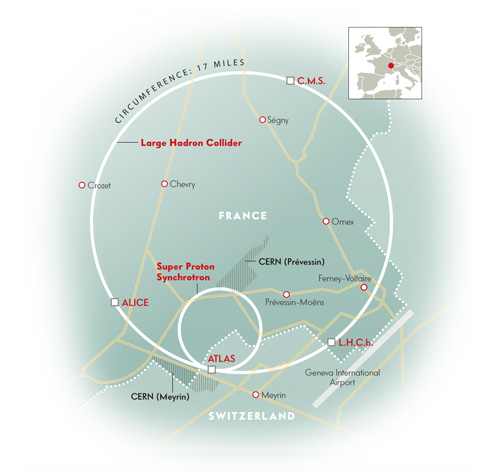
\includegraphics[width=0.99\textwidth]{figures/ch_higgs/misc/lhcring.jpg}
    }
    \caption{LHC Accelerator Complex}
    \label{fig:higgs_cms_lhc}
 \end{figure}

 The Large Hadron Collider is the particle accelerating and colliding complex located on the border between France and Switzerland. Physically speaking, it is a ring that is about 27 km in circumference and serves four major High Energy Physics Experiments: CMS, Atlas, Alice and LHCb.

\subsection{General Description} \label{subsection:higgs_cms_generaldescription}
The Compact Muon Solenoid is a two-fold creature; first of all, it is, a one of its kind, general purpose particle detector system, which consists of multiple components (to be discussed futher) and whose primary objective is to record and reconstruct physics events that could help us study the fundamental building blocks of nature. It acts like a camera, recording the footprint of the physics interactions which particle physicists use to deduce the underlying physics. The Compact Muon Solenoid is also an experiment, a collaboration of thousands of people whose combined effort made it possible to build such a device. From people involved in data-taking at Point 5 and detector maintainance experts to people performing the analysis of recorded events and making sure that the data we have collected is of the highest quality - it is one of the best examples when group effort produces results of highest estime.

The most important component of CMS that makes it stand out among other experiments is the superconducting solenoid with magnetic field of 3.8 T. The magnet is located just outside of HCAL subsystem and plays a crucial role in the overall architecture of CMS. In particular, due to the strength of magnetic field, significant improvements are expected in the search for the Higgs Boson decaying via two muons due to a high resolution of the muon system together with the power of the magnet. The closest subsystem of CMS to the interaction point is the Silicon Tracker, whose primary objective is to measure the trajectory of the charged particles passsing through. What follows are Electromagnetic and Hadronic subsystems which respectively consist of several subdetectors with varying performance characteristics. Muon Systems are located just outside of the magnet and comprise different technologies depending on the $\eta$ location.

The Large Hadron Collider is not just a challenging project from an engineering standpoint, it is also a data factory, one of its kind, that presents a unique challenge for the data processing and analysis domain. The amount of data that gets generated quickly becomes unmanagable and one has to be careful when selecting what to preserve and what to abandon. The collsion rate is about 40 MHz and the compressed size of just 1 event coming from CMS is on order of 1 KB. That amounts to 40 GB/s and if we extrapolate up to a single hour of datataking we get about 140 TB/h - obviously this becomes unfeasible very quickly. For the purpose of selection of events of interest, all HEP Experiments employ a sophisticated Trigger System, whose purpose is to select the physics events of interest. CMS has two layers of data reduction: Level 1 and High Level Trigger. Level 1 trigger system is a hardware based processing system, that is tightly integrated with the rest of the subsystems' electronics. Level 1 allows CMS to reduce the event rate from 40 MHz down to 100 KHz. This is achieved by applying basic selections at hardware level (integration with the subsystems' electronics results in zero copy processing) using reduced content information known as Trigger Primitives (TPs).

The 100 KHz output of Hardware Trigger System gets further reduced by High Level Trigger (HLC) down to 100 Hz that gets actually written to disk. This content reduction is achieved by employing high level information produced via the reconstruction procedure. Basically, CMS High Level Trigger System is a reasonable-sized High Perfomance Cluster (HPC) Complex which takes the output of Level 1 and acts as a filtering system, flagging events that should be stored to disk for offline processing. The software framework that gets used is the same one as for offline data analysis, however certain reconstruction steps are optimized for performance.

%\subsection{Tracker System} \label{subsection:higgs_cms_tracker}
%Explain Pixels and Tracker

%\subsection{Electromagnetic Calorimeter} \label{subsection:higgs_cms_em}
%Electromagnetic Calorimeter (or Ecal for breivity) is a subsystem of CMS with the primary objective to

%\subsection{Hadronic Calorimeter} \label{subsection:higgs_cms_hcal}
%Hadron Calorimeter (or Hcal for breivity) is a subsystem of CMS with the primary objective to identify and measure energy of jets. It consists of four separate parts: Hadron Barrel, Hadron Endcap, Hadron Outer and Hadron Forward.

%\subsection{Muon System} \label{subsection:higgs_cms_muon}
%Describe the Muon Systems

%\subsection{Trigger System} \label{subsection:higgs_cms_trigger}

%\subsection{Data Acquisition Software}

%\subsection{Data Analysis Software} \label{subsection:higgs_cms_cmssw}
%Describe the Software for Analysis
\section{CMS Datasets} \label{section:higgs_data}
At CMS, all of the accumulated data is organized in terms of datasets, which can be logically organized into key-value pairs. A key is the name of a dataset, which uniquely identifies it across the rest of the samples (dataset and sample are used interchangeably). At the same time, a key follows a standard naming convention, which allows to quickly resolve the most important characteristics of the actual data to which it points. A value, in turn, is a collection of data files that actually constitute the dataset and are used for the analysis.

Generally speaking, the CMS experiment produces two types of datasets: collision and simulation samples. Collision samples correspond to the actual data recorded from proton-proton collisions at the LHC. A typical collision sample name has three parts: stream identifier, timestamp and format of the data stored. Depending on the format, timestamp can either point to the actual period of datataking or the reconstruction date. The CMS assigns descriptive stream identifiers in order to provide an overview of the physical content of the events that go into a dataset. For instance, in this search, only events that have a good quality muon object are considered and a ``SingleMuon'' identifier signals exactly that. Furthermore, datasets could have identifiers like ``SingleElectron'' or ``SinglePhoton'', which would make them respectively contain events with an electron or a photon.

Simulation samples correspond to the data produced by simulating the collisions environment (production processes and subsequent decays) and the response of the CMS detector. The most important use case of the simulation is to provide a modeling baseline with which collisions data will be compared. For the purpose of the search, simulation datasets can be further divided into the signal and background samples. Signal corresponds to the Higgs Boson production processes with its subsequent decay to two muons. Backgrounds, in turn, are basically all of the processes that can produce the same signature, the same final state. A typical unique simulation sample name, similar to collision sample name, has three parts: production process specifier, conditions identifier and the format of the data stored. The first part specifies a label that summarizes the actual production process and the Monte Carlo event generators used to perform the calculations of the Feynman diagrams. Conditions part carries a label to uniquely specify a campaign when a sample is produced, software versions used, and various calibrations and corrections applied.

\subsection{Collision Datasets}
For the purpose of the search, datasets with the total integrated luminosity of 35.9 fb$^{-1}$ of CMS collision data collected over the course of 2016 datataking campaign are utilized and the full list of these samples is provided in the Table~\ref{table:higgs_data_collisiondatasets}. The signature of the search is the presence of two opposite sign muons in the event; therefore, in order to pick up as many as possible events of interest, the choice for the stream identifier is limited to either ``SingleMuon'' or ``DoubleMuon''. The choice of ``SingleMuon'' is dictated by the fact of having intrinsically higher efficiency of triggering a single muon rather than two muons per a given event. By selecting ``DoubleMuon'' trigger, for this particular search, all the events where only one muon triggers the HLT system would be thrown away. Therefore, considering that dimuon final state has a very low branching fraction for the Higgs Boson, the choice is made not to throw away the events.
\begin{table}[htb]
    \caption{Datasets used for the search from proton-proton collisions recorded at the $\sqrt{s}=13$~TeV by CMS at LHC in 2016.}
    \label{table:higgs_data_collisiondatasets}
    \begin{center}
        \begin{tabular}{ l  c}
            \hline
            Datasets & Int. Luminosity (fb$^{-1}$)\\
            \hline
            {/SingleMuon/Run2016B-03Feb2017\_ver2-v2/MINIAOD} & 5.788\\
            {/SingleMuon/Run2016C-03Feb2017-v1/MINIAOD} & 2.573\\
            {/SingleMuon/Run2016D-03Feb2017-v1/MINIAOD} & 4.248\\
            {/SingleMuon/Run2016E-03Feb2017-v1/MINIAOD} & 4.009\\
            {/SingleMuon/Run2016F-03Feb2017-v1/MINIAOD} & 3.102\\
            {/SingleMuon/Run2016G-03Feb2017-v1/MINIAOD} & 7.540\\
            {/SingleMuon/Run2016H-03Feb2017\_ver2(3)-v1/MINIAOD} & 8.606\\
            \hline
        \end{tabular}
    \end{center}
\end{table}

\subsection{Signal Datasets}
For the purpose of testing various hypothetical Standard Model Higgs Boson masses, it is crucial to be able to build signal models for each hypothesis. In this analysis, samples with three different hypothetical Higgs Boson masses are used, 120/125/130 GeV, which allows a mass range [120, 130] GeV to be examined. The process of signal model construction and interpolation of parameters as a function of the Higgs Boson mass is discussed in further detail in Section~\ref{section:higgs_signalmodel}. The choice of the mass range is driven by the evidence obtained from searches for the Higgs Boson in other final states, discussed in Section~\ref{section:higgs_run1results}, where observations of a resonance near 125 GeV mass were made. Table~\ref{table:higgs_data_signaldatasets} provides a summary of the CMS signal samples used along with cross section of each production process for the 125 GeV mass hypothesis.
\begin{table}[htb]
    \caption{Standard Model 125 GeV Higgs Boson Signal Datasets for 13 TeV. Dataset names for 120/130 GeV are omitted for brevity. Moriond 2017 conditions are used (omitted the conditions specification for brevity).}
    \label{table:higgs_data_signaldatasets}
        \begin{center}
        \begin{tabular}{ l  c}
            \hline
            Datasets & $\sigma$ (pb)\\
            \hline
            {/GluGlu\_HToMuMu\_M125\_13TeV\_powheg\_pythia8} & 48.58\\
            {/VBF\_HToMuMu\_M125\_13TeV\_powheg\_pythia8} & 3.782\\
            {/WMinusH\_HToMuMu\_M125\_13TeV\_powheg\_pythia8} & 0.5331\\
            {/WPlusH\_HToMuMu\_M125\_13TeV\_powheg\_pythia8} & 0.851\\
            {/ZH\_HToMuMu\_M125\_13TeV\_powheg\_pythia8} & 0.8839 \\
            \hline
        \end{tabular}
        \end{center}
\end{table}
The Higgs signal production processes considered in this search are gluon
fusion (ggH), vector boson fusion (VBF), Higgsstrahlung (VH). Production in
association with top quarks (\ttH) has been generated privately. The Higgs MC samples are generated using {\sc POWHEG}~\cite{Nason:2004rx}.

\subsection{Background Datasets}
As it has already been stated, background processes are the processes that result in the same final state (at least two muons in the event) as the Higgs Boson samples considered. For this analysis, all the processes that produce two muons in the final state, but not through their coupling to the Higgs field,  are to be considered backgrounds. Table~\ref{table:higgs_data_backgrounddatasets} provides a summary of the most dominant contributions among the background processes. The largest contributor is the Drell-Yan process, which constitutes approximately 90\% of background events, and has a pair of leptons in the final state. The next-to-leading contributor is the $\mathrm{t\bar{t}}$ production, with subsequent decay of top quarks into lighter bottom quarks and W$^{\pm}$ vector bosons further coupling to two fermions. These two mechanisms are responsible for more than 98\% of background events contributing to the dimuon final state.
\begin{table}[htb]
    \caption{Background Datasets. Moriond 2017 conditions have been used (omitted the conditions specification for brevity).}
    \label{table:higgs_data_backgrounddatasets}
    \begin{center}
        \begin{tabular}{ l  c}
            \hline
            Dataset & $\sigma$ (pb)\\
            \hline
            /DYJetsToLL\_M-50\_TuneCUETP8M1\_13TeV-amcatnloFXFX-pythia8 & 5765\\
            /ST\_tW\_top\_5f\_NoFullyHadronicDecays\_13TeV-powheg\_TuneCUETP8M1 & 35.85\\
            /TTJets\_DiLept\_TuneCUETP8M1\_13TeV-madgraphMLM-pythia8 & 85.656\\
            /WJetsToLNu\_TuneCUETP8M1\_13TeV-amcatnloFXFX-pythia8 & 61526.7\\
            /WWTo2L2Nu\_13TeV-powheg-herwigpp & 10.481\\
            /WZTo3LNu\_TuneCUETP8M1\_13TeV-amcatnloFXFX-pythia8 & 4.712\\
            \hline
        \end{tabular}
    \end{center}
\end{table}

Depending on the analysis strategy, the role of background simulation samples can be two fold. First, they are used for comparison with collision data, in particular to make sure that dimuon mass is well-modeled by the included backgrounds. The idea is to show that physical quantities of interest (dimuon mass, various kinematic variables) are in line with theoretical predictions. It is important to point out that both data and simulated samples will be further subject to exactly the same selections, further described in Section~\ref{section:higgs_selections}. Second, background datasets can be directly used for the hypothesis testing and statistical analysis of the presence of the signal in the data. In such a case, it is common to abbreviate this approach as simulation driven, because the simulated background dimuon mass distributions are directly used in the hypothesis testing. Another approach, commonly named data driven, is to build a model, similar to the construction of a signal model and discussed further in Section~\ref{section:higgs_bkgmodel}, that will be fit to the actual data, constrained and used to estimate the background yield.

This analysis follows a data-driven background estimation approach due to the low statistical power of simulated background samples. In other words, significant bin-to-bin fluctuations are present, especially for the categories with lower statistics, that would result in inadequate extraction of the upper limits. Therefore, the primary use of background datasets is to compare various kinematic variable distributions from data and theoretical predictions. Moreover, as it will be clarified in Section~\ref{section:higgs_categorization}, depending on the categorization technique used, background samples will be further used for training a binary classification algorithm for the purpose of signal discrimination.

Single top samples are generated with {\sc POWHEG}, whereas $\mathrm{t\bar{t}}$ samples and the multi-boson samples are generated either with {\sc madgrapgh}~\cite{Alwall:2011uj} or {\sc amc@NLO} (Next to Leading Order)~\cite{amcatnlo}. Spin effects in multiboson processes are simulated using {\sc Madspin}. The parton shower and hadronization processes are modeled by the {\sc Pythia8} generator~\cite{Sjostrand:2007gs} with TuneCUETP8M1.

%The simulated pile up distribution is reweighted to match the observed
%distribution in data for all MC samples.

% \begin{table}[!h]
% \small
% \renewcommand{\arraystretch}{1.5}

% \begin{tabular}{|l||l|c|}
%     \hline \textbf{Dataset} & Run Range & Integrated Luminosity \\
%     \hline  &  & [fb$^{-1}$] \\
%     \hline
%         %% %% Fairly certain ver1-v1 is not used at all (no events in Golden JSON - AWB 13.05.16
%     %% \hline \url{/SingleMuon/Run2016B-03Feb2017_ver1-v1/MINIAOD} & \multirow{2}{*}{272007-275376} & \multirow{2}{*}{5.788} \\ \cline{1-1}
%     %% \url{/SingleMuon/Run2016B-03Feb2017_ver2-v2/MINIAOD} &  &  \\
%         \hline \url{/SingleMuon/Run2016B-03Feb2017_ver2-v2/MINIAOD} & 272007-275376 & 5.788 \\
%     \hline \url{/SingleMuon/Run2016C-03Feb2017-v1/MINIAOD}      & 275657-276283 & 2.573 \\
%     \hline \url{/SingleMuon/Run2016D-03Feb2017-v1/MINIAOD}      & 276315-276811 & 4.248 \\
%     \hline \url{/SingleMuon/Run2016E-03Feb2017-v1/MINIAOD}      & 276831-277420 & 4.009 \\
%     \hline \url{/SingleMuon/Run2016F-03Feb2017-v1/MINIAOD}      & 277772-278808 & 3.102 \\
%         \hline \url{/SingleMuon/Run2016G-03Feb2017-v1/MINIAOD}      & 278820-280385 & 7.540 \\
%     \hline \url{/SingleMuon/Run2016H-03Feb2017_ver2-v1/MINIAOD} & \multirow{2}{*}{280919-284044} & \multirow{2}{*}{8.606} \\ \cline{1-1}
%            \url{/SingleMuon/Run2016H-03Feb2017_ver3-v1/MINIAOD} &                                &                        \\
%     \hline                                                         %% Adds up to 35.866 - i.e. 35.9 fb^-1
%     \hline \multicolumn{3}{|l|}{\textbf{Luminosity mask: \url{Cert_271036-284044_13TeV_23Sep2016ReReco_Collisions16_JSON.txt}}}    \\
% \hline
% \end{tabular}

% \caption{Overview of the single muon data stream collected during the
% proton-proton collisions at $\sqrt{s}=13$~TeV by CMS at LHC in 2016.}
% \label{tab:datasets}
% \end{table}

% \newpage
% \begin{landscape}
% \begin{table}[p]
% \renewcommand{\arraystretch}{1.5}
% \tiny
% \begin{tabular}{|l||c|c|c|}
%   \hline \textbf{Higgs signal MC samples} & Events & Cross section [pb] & Xsec $\times$ BR [fb]  \\
%   %% From Yellow Report 4 (https://arxiv.org/abs/1610.07922), H --> mu-mu branching ratio at 125 GeV = 0.0002176
%   %% ggH = 48.58 pb, VBF = 3.7817 pb, W+H = 0.09426 pb, W-H = 0.05983 pb, ZH = 0.17762 pb, ttH = 0.5071 pb
%   \hline
%   \hline \url{/GluGlu_HToMuMu_M125_13TeV_powheg_pythia8/RunIISummer16MiniAODv2-PUMoriond17_80X_mcRun2_asymptotic_2016_TrancheIV_v6-v1/MINIAODSIM }  &  250000 & 48.58    & 10.571   \\
%   \hline \url{/VBF_HToMuMu_M125_13TeV_powheg_pythia8/RunIISummer16MiniAODv2-PUMoriond17_80X_mcRun2_asymptotic_2016_TrancheIV_v6-v1/MINIAODSIM }     &  249200 &  3.7817  & 0.8229   \\
%   \hline \url{/WPlusH_HToMuMu_M125_13TeV_powheg_pythia8/RunIISummer16MiniAODv2-PUMoriond17_80X_mcRun2_asymptotic_2016_TrancheIV_v6-v1/MINIAODSIM }  &  124547 &  0.09426 & 0.02051  \\
%   \hline \url{/WMinusH_HToMuMu_M125_13TeV_powheg_pythia8/RunIISummer16MiniAODv2-PUMoriond17_80X_mcRun2_asymptotic_2016_TrancheIV_v6-v1/MINIAODSIM } &  125000 &  0.05983 & 0.013019 \\
%   \hline \url{/ZH_HToMuMu_M125_13TeV_powheg_pythia8/RunIISummer16MiniAODv2-PUMoriond17_80X_mcRun2_asymptotic_2016_TrancheIV_v6-v1/MINIAODSIM }      &  249748 &  0.17762 & 0.03865  \\
%   %% \hline \url{/ttHToNonbb_M125_TuneCUETP8M2_ttHtranche3_13TeV-powheg-pythia8/RunIISummer16MiniAODv2-PUMoriond17_80X_mcRun2_asymptotic_2016_TrancheIV_v6-v1/MINIAODSIM } & 3981250 & 0.5071 & 0.11034 \\

% \hline
% \end{tabular}

% \caption{The Higgs signal MC samples were generated with {\sc POWHEG}
% while the parton shower and hadronization processes are modeled by the
% {\sc Phythia8} generator with TuneCUETP8M1.}
% \label{tab:SignalMC}
% \end{table}
% \end{landscape}

% \newpage
% \begin{landscape}
% \begin{table}[p]
% \tiny
% \renewcommand{\arraystretch}{1.2}
% \begin{tabular}{|l||c|c|}
%     \hline \textbf{Background MC} & Events & Cross Section [pb]  \\
%     \hline
%     \hline \multicolumn{3}{|c|}{\textbf{Drell--Yan}}  \\
%     \hline
%     \hline \url{/DYJetsToLL_M-50_TuneCUETP8M1_13TeV-amcatnloFXFX-pythia8/RunIISummer16MiniAODv2-PUMoriond17_80X_mcRun2_asymptotic_2016_TrancheIV_v6_ext2-v1/MINIAODSIM} &  122055388 & 5765  \\
%     \hline \url{/DYToLL_0J_13TeV-amcatnloFXFX-pythia8/RunIISummer16MiniAODv2-PUMoriond17_80X_mcRun2_asymptotic_2016_TrancheIV_v6_ext1-v1/MINIAODSIM} & 49579613  &  4754\\
%     %% \hline \url{/DYToLL_0J_13TeV-amcatnloFXFX-pythia8/RunIISummer16MiniAODv2-PUMoriond17_backup_80X_mcRun2_asymptotic_2016_TrancheIV_v6-v1/MINIAODSIM} & 44253240  &  4754    \\
%     \hline \url{/DYToLL_1J_13TeV-amcatnloFXFX-pythia8/RunIISummer16MiniAODv2-PUMoriond17_80X_mcRun2_asymptotic_2016_TrancheIV_v6_ext1-v1/MINIAODSIM} & 49902571  & 888.9 \\
%     %% \hline \url{/DYToLL_1J_13TeV-amcatnloFXFX-pythia8/RunIISummer16MiniAODv2-PUMoriond17_backup_80X_mcRun2_asymptotic_2016_TrancheIV_v6-v1/MINIAODSIM} & 41597712  & 888.9 \\
%     \hline \url{/DYToLL_2J_13TeV-amcatnloFXFX-pythia8/RunIISummer16MiniAODv2-PUMoriond17_80X_mcRun2_asymptotic_2016_TrancheIV_v6-v2/MINIAODSIM} & 42324802  & 348.8 \\
%     \hline \url{/DYToLL_2J_13TeV-amcatnloFXFX-pythia8/RunIISummer16MiniAODv2-PUMoriond17_80X_mcRun2_asymptotic_2016_TrancheIV_v6_ext1-v1/MINIAODSIM} & 47974554  & 348.8 \\
%     %% \hline \url{/DYJetsToLL_M-100to200_TuneCUETP8M1_13TeV-amcatnloFXFX-pythia8/RunIISummer16MiniAODv2-PUMoriond17_80X_mcRun2_asymptotic_2016_TrancheIV_v6_ext1-v1/MINIAODSIM} &  1083606 &  ??? \\
%     \hline
%     \hline \multicolumn{3}{|c|}{\textbf{SingleTop}}    \\
%     \hline
%     \hline \url{/ST_tW_top_5f_NoFullyHadronicDecays_13TeV-powheg_TuneCUETP8M1/RunIISummer16MiniAODv2-PUMoriond17_80X_mcRun2_asymptotic_2016_TrancheIV_v6-v1/MINIAODSIM} & 5372991  & 35.85 \\
%     \hline \url{/ST_tW_top_5f_NoFullyHadronicDecays_13TeV-powheg_TuneCUETP8M1/RunIISummer16MiniAODv2-PUMoriond17_80X_mcRun2_asymptotic_2016_TrancheIV_v6_ext1-v1/MINIAODSIM} & 3256650  & 35.85 \\
%     \hline \url{/ST_tW_antitop_5f_NoFullyHadronicDecays_13TeV-powheg_TuneCUETP8M1/RunIISummer16MiniAODv2-PUMoriond17_80X_mcRun2_asymptotic_2016_TrancheIV_v6-v1/MINIAODSIM} & 5425134  & 35.85 \\
%     \hline \url{/ST_tW_antitop_5f_NoFullyHadronicDecays_13TeV-powheg_TuneCUETP8M1/RunIISummer16MiniAODv2-PUMoriond17_80X_mcRun2_asymptotic_2016_TrancheIV_v6_ext1-v1/MINIAODSIM} & 3256407 & 35.85 \\
%     \hline
%     \hline \multicolumn{3}{|c|}{\textbf{TopPair}}    \\
%     \hline
%     \hline \url{/TTJets_DiLept_TuneCUETP8M1_13TeV-madgraphMLM-pythia8/RunIISummer16MiniAODv2-PUMoriond17_80X_mcRun2_asymptotic_2016_TrancheIV_v6-v1/MINIAODSIM} & 6094476 & 85.656 \\
%     \hline \url{/TTJets_DiLept_TuneCUETP8M1_13TeV-madgraphMLM-pythia8/RunIISummer16MiniAODv2-PUMoriond17_80X_mcRun2_asymptotic_2016_TrancheIV_v6_ext1-v1/MINIAODSIM} & 24350202  & 85.656 \\
%     \hline \url{/TTJets_Dilept_TuneCUETP8M2T4_13TeV-amcatnloFXFX-pythia8/RunIISummer16MiniAODv2-PUMoriond17_80X_mcRun2_asymptotic_2016_TrancheIV_v6-v1/MINIAODSIM} &  14529280 & 85.656  \\
%     \hline
%     \hline \multicolumn{3}{|c|}{\textbf{DiBoson}}    \\
%     \hline
%     \hline \url{/WWTo2L2Nu_13TeV-powheg/RunIISummer16MiniAODv2-PUMoriond17_80X_mcRun2_asymptotic_2016_TrancheIV_v6-v1/MINIAODSIM } & 1999000  & 12.46  \\
%     \hline \url{/WZTo3LNu_TuneCUETP8M1_13TeV-amcatnloFXFX-pythia8/RunIISummer16MiniAODv2-PUMoriond17_80X_mcRun2_asymptotic_2016_TrancheIV_v6-v1/MINIAODSIM} & 11887464  & 2.113 \\
%     \hline \url{/WZTo2L2Q_13TeV_amcatnloFXFX_madspin_pythia8/RunIISummer16MiniAODv2-PUMoriond17_80X_mcRun2_asymptotic_2016_TrancheIV_v6-v1/MINIAODSIM} & 26517272  &  4.409 \\
%     \hline \url{/ZZTo2L2Nu_13TeV_powheg_pythia8/RunIISummer16MiniAODv2-PUMoriond17_80X_mcRun2_asymptotic_2016_TrancheIV_v6-v1/MINIAODSIM} & 8842475  & 0.564  \\
%     \hline \url{/ZZTo2L2Q_13TeV_amcatnloFXFX_madspin_pythia8/RunIISummer16MiniAODv2-PUMoriond17_80X_mcRun2_asymptotic_2016_TrancheIV_v6-v1/MINIAODSIM} & 15345572  & 3.22 \\
%     \hline \url{/ZZTo4L_13TeV-amcatnloFXFX-pythia8/RunIISummer16MiniAODv2-PUMoriond17_80X_mcRun2_asymptotic_2016_TrancheIV_v6_ext1-v1/MINIAODSIM} &  10709784 & 1.212  \\
%     \hline
%     \hline \multicolumn{3}{|c|}{\textbf{TriBoson}}   \\
%     \hline
%     \hline \url{/WWW_4F_TuneCUETP8M1_13TeV-amcatnlo-pythia8/RunIISummer16MiniAODv2-PUMoriond17_80X_mcRun2_asymptotic_2016_TrancheIV_v6-v1/MINIAODSIM } & 240000   &     0.2086  \\
%     \hline \url{/WWZ_TuneCUETP8M1_13TeV-amcatnlo-pythia8/RunIISummer16MiniAODv2-PUMoriond17_80X_mcRun2_asymptotic_2016_TrancheIV_v6-v1/MINIAODSIM} & 250000  & 0.1651 \\
%     \hline \url{/WZZ_TuneCUETP8M1_13TeV-amcatnlo-pythia8/RunIISummer16MiniAODv2-PUMoriond17_80X_mcRun2_asymptotic_2016_TrancheIV_v6-v1/MINIAODSIM} & 246800  & 0.05565 \\
%     \hline \url{/ZZZ_TuneCUETP8M1_13TeV-amcatnlo-pythia8/RunIISummer16MiniAODv2-PUMoriond17_80X_mcRun2_asymptotic_2016_TrancheIV_v6-v1/MINIAODSIM} & 249237  & 0.01398 \\
%     \hline
%     \hline \multicolumn{3}{|c|}{\textbf{SingleTop+X}}    \\
%     \hline
%     \hline \url{/tZq_ll_4f_13TeV-amcatnlo-pythia8/RunIISummer16MiniAODv2-PUMoriond17_80X_mcRun2_asymptotic_2016_TrancheIV_v6_ext1-v1/MINIAODSIM } & 14509520  & 0.0758  \\
%     %\hline \url{/ST_tWll_5f_LO_13TeV-MadGraph-pythia8/RunIISummer16MiniAODv2-PUMoriond17_80X_mcRun2_asymptotic_2016_TrancheIV_v6-v1/MINIAODSIM} &  50000 & ??? \\
%     \hline
%     \hline \multicolumn{3}{|c|}{\textbf{Top pairs}}    \\
%     \hline
%     \hline \url{/TTWJetsToLNu_TuneCUETP8M1_13TeV-amcatnloFXFX-madspin-pythia8/RunIISummer16MiniAODv2-PUMoriond17_80X_mcRun2_asymptotic_2016_TrancheIV_v6_ext1-v3/MINIAODSIM     } & 2160168  & 0.2043 \\
%     \hline \url{/TTWJetsToLNu_TuneCUETP8M1_13TeV-amcatnloFXFX-madspin-pythia8/RunIISummer16MiniAODv2-PUMoriond17_80X_mcRun2_asymptotic_2016_TrancheIV_v6_ext2-v1/MINIAODSIM} & 3120397  & 0.2043 \\
%     \hline \url{/TTZToLLNuNu_M-10_TuneCUETP8M1_13TeV-amcatnlo-pythia8/RunIISummer16MiniAODv2-PUMoriond17_80X_mcRun2_asymptotic_2016_TrancheIV_v6_ext1-v1/MINIAODSIM} & 1992438  & 0.2529 \\

% \hline

% \end{tabular}

% \caption{The MC background processes samples were generated with {amc@NLO}.
% {\sc POWHEG} and {\sc madgrapgh}. Spin effects in multi boson processes are
% simulated using  {\sc madspin}. The parton shower and hadronization processes
%  are modeled by the {\sc Phythia8} generator with TuneCUETP8M1.}
% \label{tab:BkgMC}
% \end{table}
% \end{landscape}

%\subsection{Pileup Reweighting}
%\label{pu}

% Each MC samples is reweighted in order to match the pileup distribution in data, as centrally recommended using the ``minimum bias'' cross section of $69.2$mb $\pm5\%$.
% The value needs to be read as an effective minimum bias times efficiesies cross section with respect to what present in pythia8; large uncertainties are present in order to cover differences between the run period and the charge/neutral compenents.

% \begin{figure}[h!]
%     \centering
%     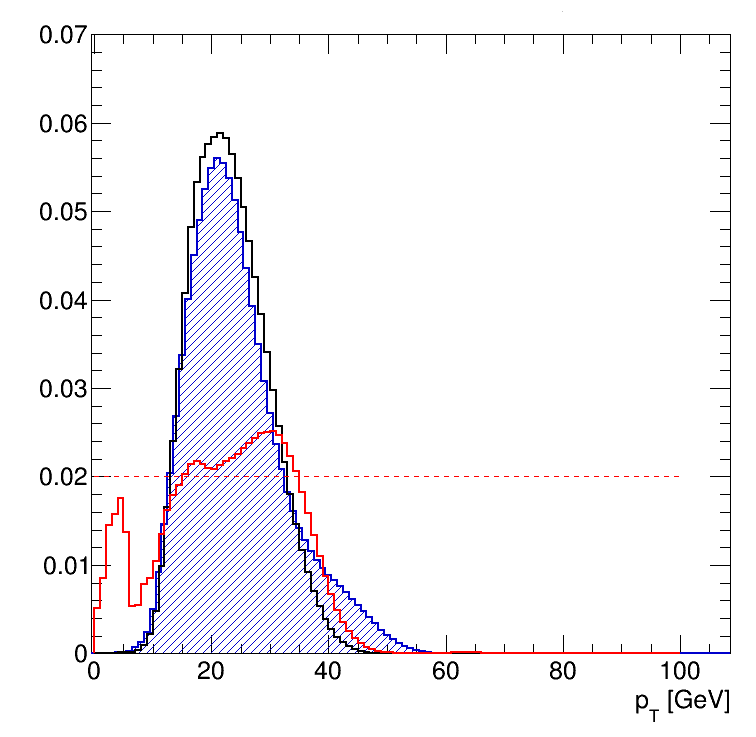
\includegraphics[width=0.49\textwidth]{figures/data_mc_samps/Pu-reweight2.png}
%     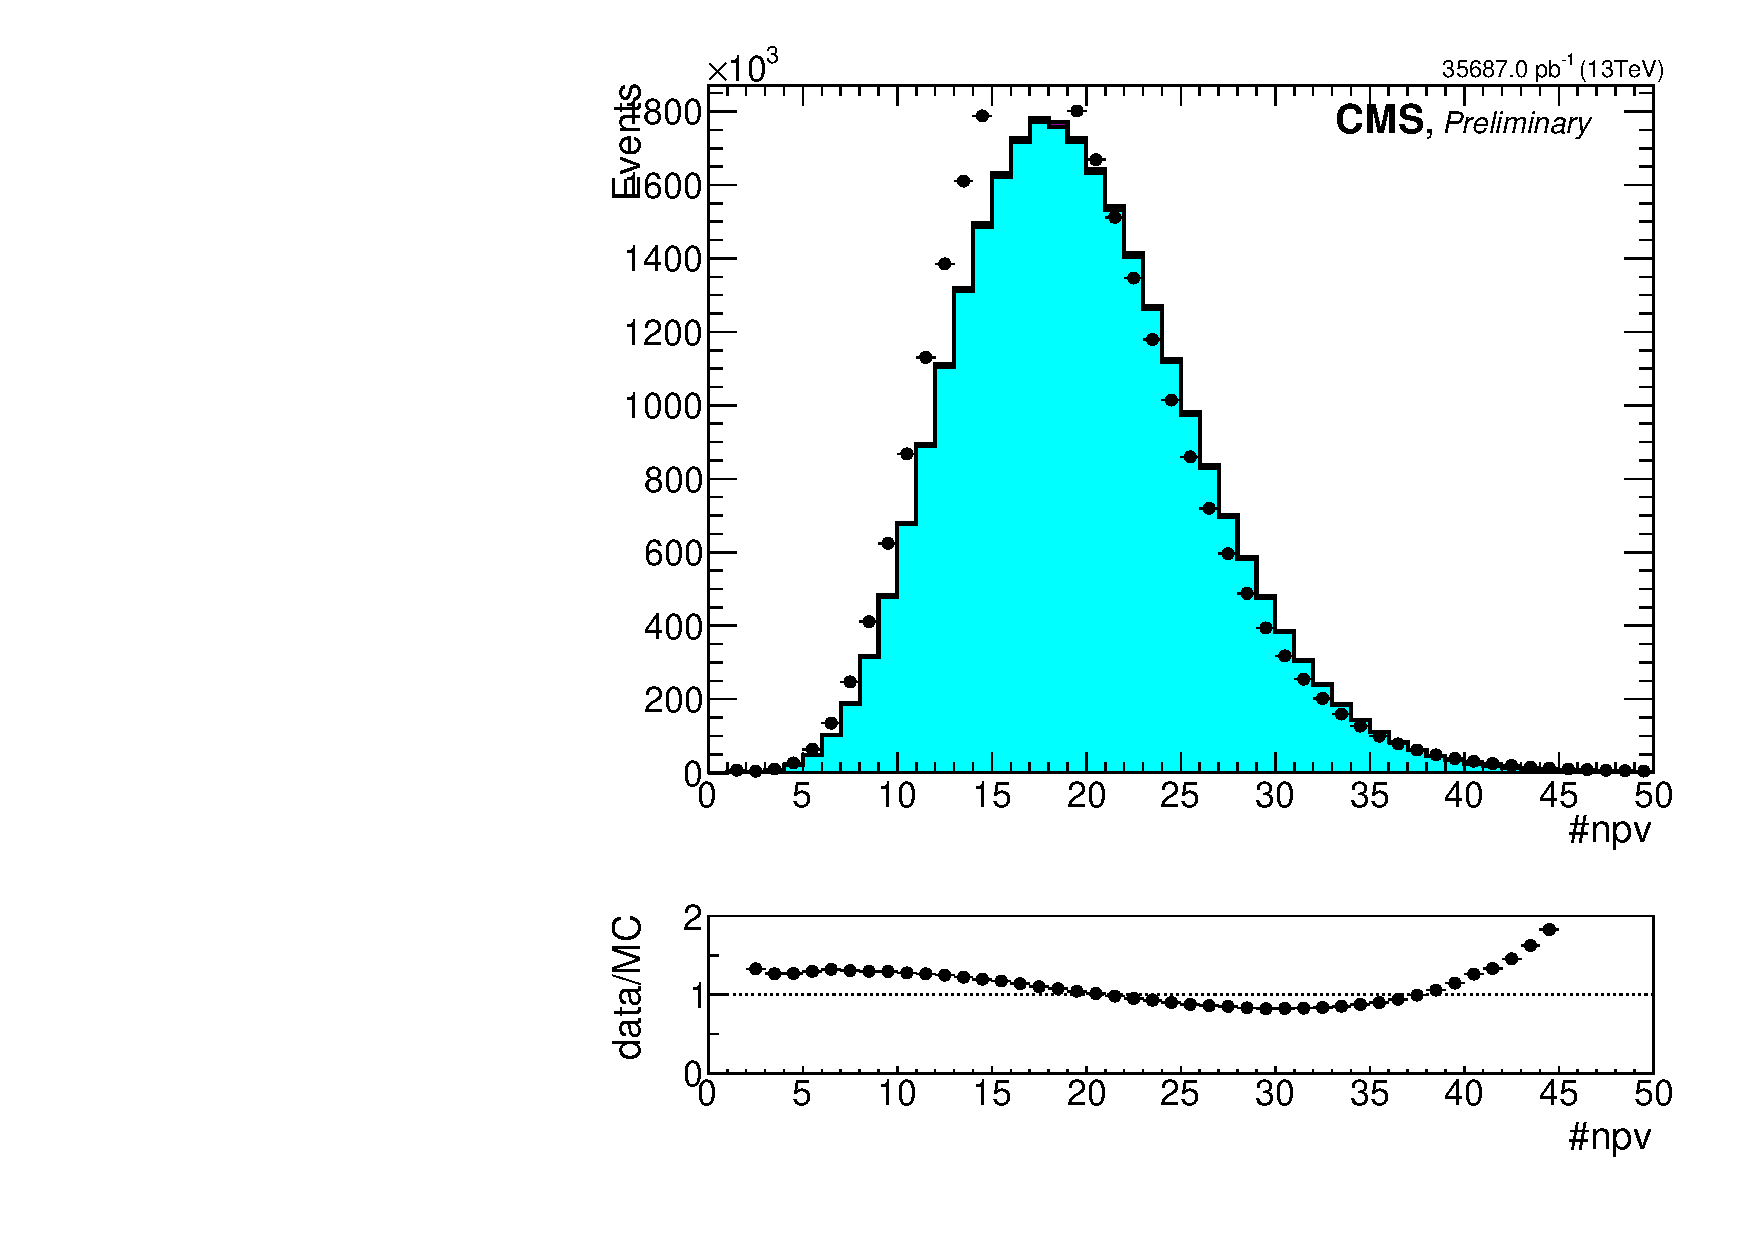
\includegraphics[width=0.49\textwidth]{figures/data_mc_samps/mmNpv_pileup69200.pdf}\\
%     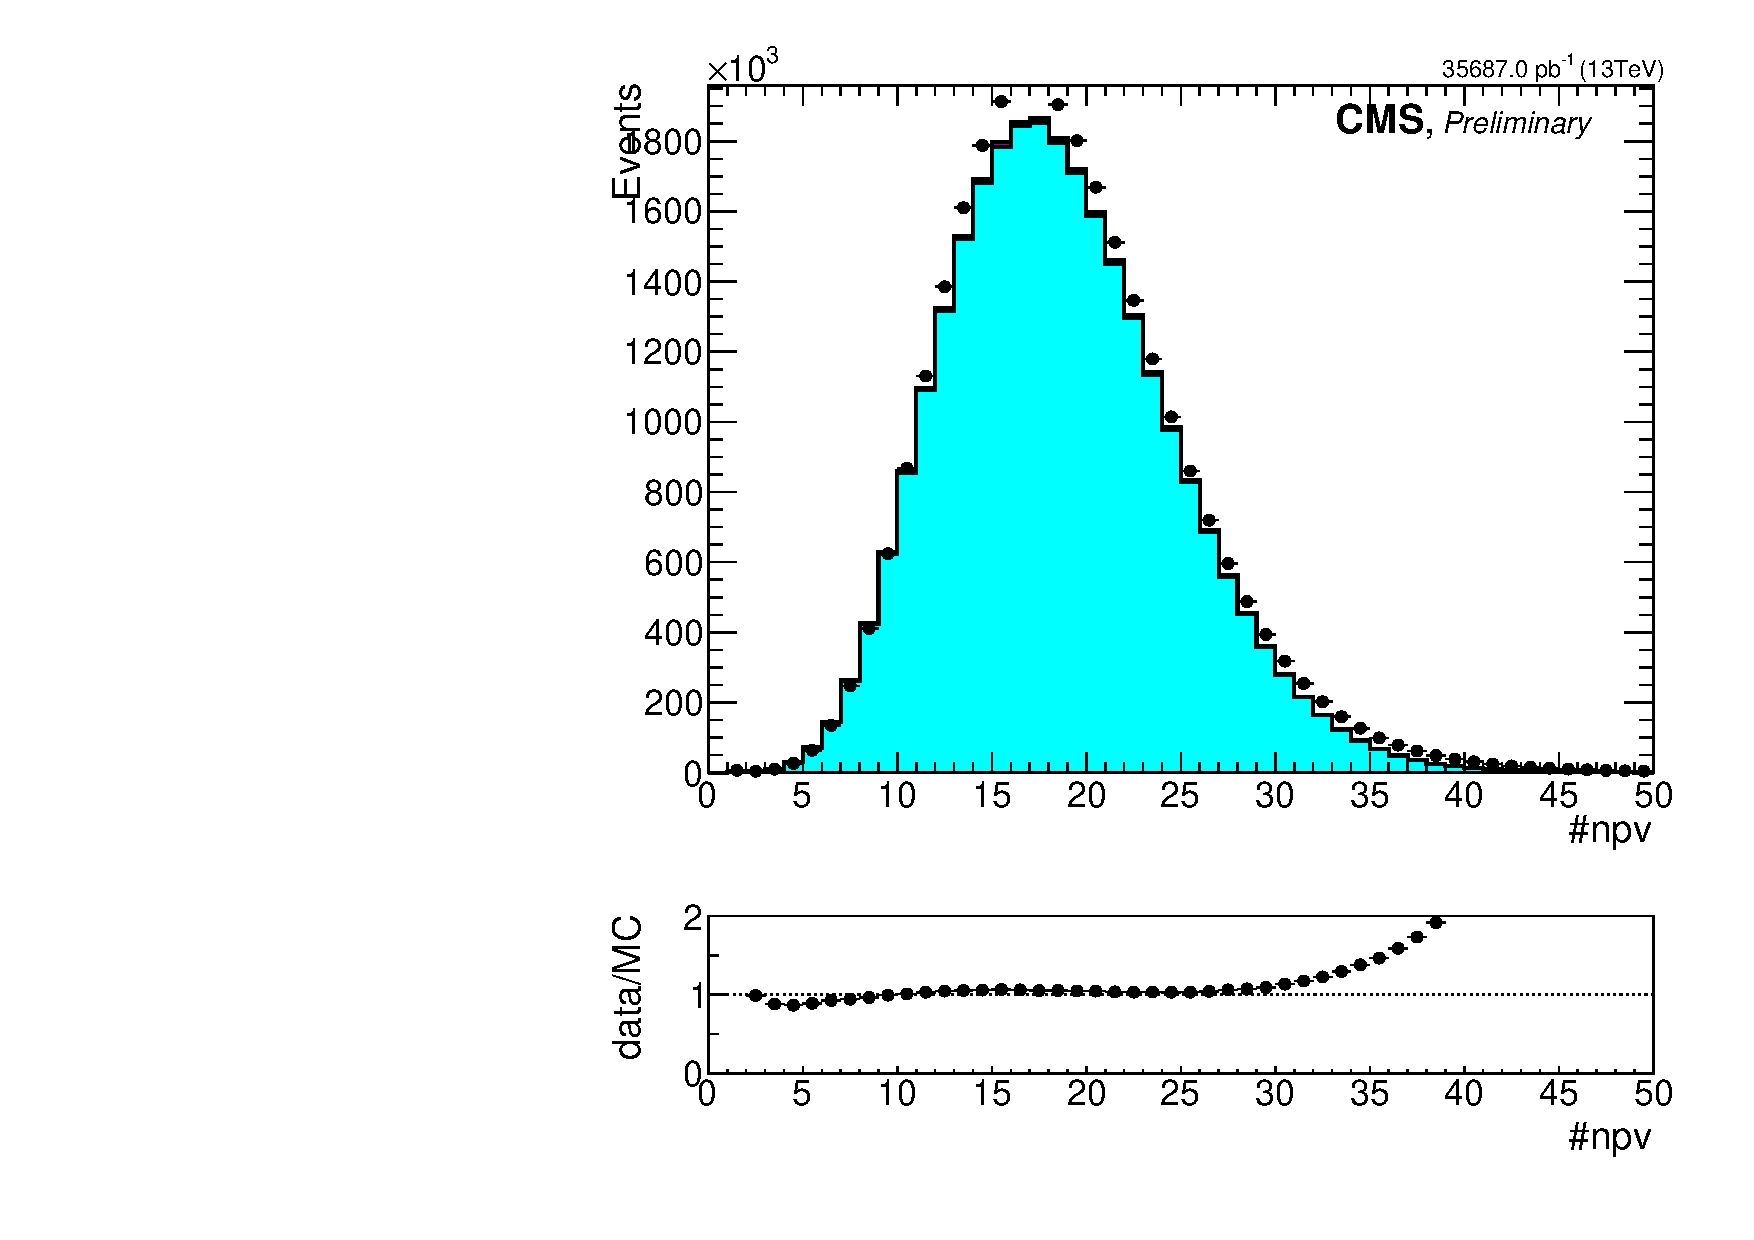
\includegraphics[width=0.49\textwidth]{figures/data_mc_samps/mmNpv_pileup65000.pdf}
%     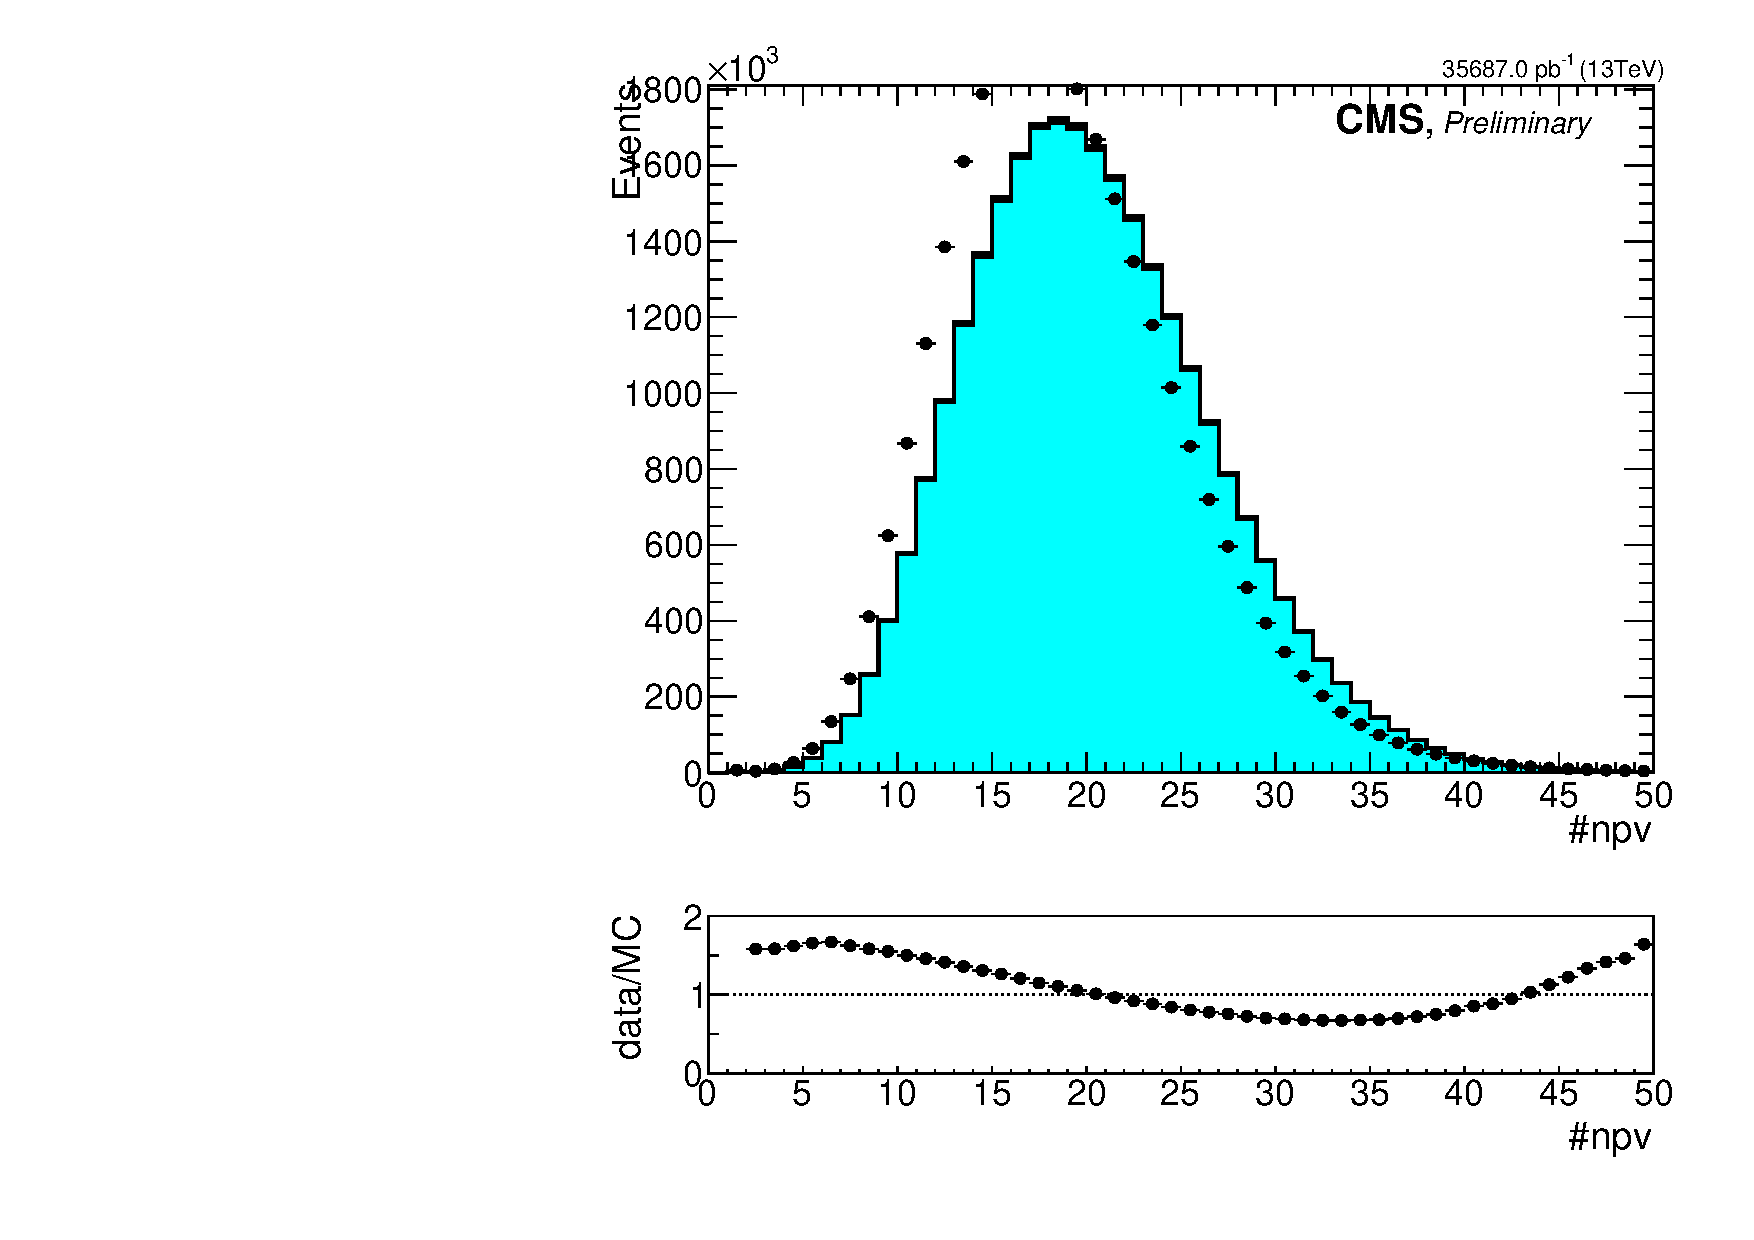
\includegraphics[width=0.49\textwidth]{figures/data_mc_samps/mmNpv_pileup72000.pdf}
%     \caption{Top Left. Pileup reweighting factors, data and MC truth pileup distributions. Top Right. agreement in the number of primary vertex variable after pu-reweighting. Bottom. agreement for the n.p.v. variables after $\pm1\sigma$ uncertainty in the pu-reweighting cress section.}
% \end{figure}




%\section{CMS Monte-Carlo Datasets} \label{section:higgs_mc}


\subsection{Signal Samples} \label{subsection:higgs_mc_signal}
We use Signal Samples with three different hypothetical Standard Model Higgs Boson masses. Since we are performing a search and are leaving the mass floating, we need a way to probe various hypotheses. Using three mass points (samples) we can model parameters for a given model and further perform interpolation to deduce the parameters for any mass that falls within our range.

\begin{table}[!h]
    \caption{Signal Samples}
    \label{table:higgs_mc_signal}
    \begin{center}
        \begin{tabular}{|l|l|}
            \hline
            Dataset & Mass\\
            \hline
            /GluGlu\_HToMuMu\_M120\_13TeV\_powheg\_pythia8/\\RunIISummer16MiniAODv2-PUMoriond17\_80X\_mcRun2\_asymptotic\_2016\_\\TrancheIV\_v6-v1/MINIAODSIM & 120 GeV\\
            /GluGlu\_HToMuMu\_M125\_13TeV\_powheg\_pythia8/\\RunIISummer16MiniAODv2-PUMoriond17\_80X\_\\mcRun2\_asymptotic\_2016\_TrancheIV\_v6-v1/MINIAODSIM & 125 GeV\\
            /GluGlu\_HToMuMu\_M130\_13TeV\_powheg\_pythia8/\\RunIISummer16MiniAODv2-PUMoriond17\_80X\_mcRun2\_asymptotic\_2016\_\\TrancheIV\_v6-v1/MINIAODSIM & 130 GeV\\
            \hline
            /VBF\_HToMuMu\_M120\_13TeV\_powheg\_pythia8/\\RunIISummer16MiniAODv2-PUMoriond17\_80X\_\\mcRun2\_asymptotic\_2016\_TrancheIV\_v6-v1/MINIAODSIM & 120 GeV\\
            /VBF\_HToMuMu\_M125\_13TeV\_powheg\_pythia8/\\RunIISummer16MiniAODv2-PUMoriond17\_80X\_\\mcRun2\_asymptotic\_2016\_TrancheIV\_v6-v1/MINIAODSIM & 125 GeV\\
            /VBF\_HToMuMu\_M130\_13TeV\_powheg\_pythia8/\\RunIISummer16MiniAODv2-PUMoriond17\_80X\_\\mcRun2\_asymptotic\_2016\_TrancheIV\_v6-v1/MINIAODSIM & 130 GeV\\
            \hline
            /WMinusH\_HToMuMu\_M120\_13TeV\_powheg\_pythia8/\\RunIISummer16MiniAODv2-PUMoriond17\_80X\_\\mcRun2\_asymptotic\_2016\_TrancheIV\_v6-v1/MINIAODSIM & 120 GeV\\
            /WMinusH\_HToMuMu\_M125\_13TeV\_powheg\_pythia8/\\RunIISummer16MiniAODv2-PUMoriond17\_80X\_\\mcRun2\_asymptotic\_2016\_TrancheIV\_v6-v1/MINIAODSIM & 125 GeV\\
            /WMinusH\_HToMuMu\_M130\_13TeV\_powheg\_pythia8/\\RunIISummer16MiniAODv2-PUMoriond17\_80X\_\\mcRun2\_asymptotic\_2016\_TrancheIV\_v6-v1/MINIAODSIM & 130 GeV\\
            \hline
            /WPlusH\_HToMuMu\_M120\_13TeV\_powheg\_pythia8/\\RunIISummer16MiniAODv2-PUMoriond17\_80X\_\\mcRun2\_asymptotic\_2016\_TrancheIV\_v6-v1/MINIAODSIM & 120 GeV\\
            /WPlusH\_HToMuMu\_M125\_13TeV\_powheg\_pythia8/\\RunIISummer16MiniAODv2-PUMoriond17\_80X\_\\mcRun2\_asymptotic\_2016\_TrancheIV\_v6-v1/MINIAODSIM & 125 GeV\\
            /WPlusH\_HToMuMu\_M130\_13TeV\_powheg\_pythia8/\\RunIISummer16MiniAODv2-PUMoriond17\_80X\_\\mcRun2\_asymptotic\_2016\_TrancheIV\_v6-v1/MINIAODSIM & 130 GeV\\
            \hline
            /ZH\_HToMuMu\_M120\_13TeV\_powheg\_pythia8/\\RunIISummer16MiniAODv2-PUMoriond17\_80X\_\\mcRun2\_asymptotic\_2016\_TrancheIV\_v6-v1/MINIAODSIM & 120 GeV\\
            /ZH\_HToMuMu\_M125\_13TeV\_powheg\_pythia8/\\RunIISummer16MiniAODv2-PUMoriond17\_80X\_\\mcRun2\_asymptotic\_2016\_TrancheIV\_v6-v1/MINIAODSIM & 125 GeV\\
            /ZH\_HToMuMu\_M130\_13TeV\_powheg\_pythia8/\\RunIISummer16MiniAODv2-PUMoriond17\_80X\_\\mcRun2\_asymptotic\_2016\_TrancheIV\_v6-v1/MINIAODSIM & 130 GeV\\
            \hline
        \end{tabular}
    \end{center}
\end{table}

\subsection{Background Samples} \label{subsection:higgs_mc_background}
Table~\ref{table:higgs_mc_background} provides a summary of the most dominant contributions among the background processes. Given that we use data-driven approach for our search, background samples are not used in any of the statistical modeling. However, the primary use of background datasets is to compare various kinematic variable distributions from data and theoretical predictions in section~\ref{section:higgs_results}

\begin{table}[!h]
    \caption{Background Samples}
    \label{table:higgs_mc_background}
    \begin{center}
        \begin{tabular}{|l|}
            \hline
            Dataset\\
            \hline
            /DYJetsToLL\_M-50\_TuneCUETP8M1\_13TeV-amcatnloFXFX-pythia8/RunIISummer16MiniAODv2-PUMoriond17\_HCALDebug\_80X\_mcRun2\_asymptotic\_2016\_TrancheIV\_v6-v1/MINIAODSIM\\
            /TTJets\_DiLept\_TuneCUETP8M1\_13TeV-madgraphMLM-pythia8/RunIISummer16MiniAODv2-PUMoriond17\_80X\_mcRun2\_asymptotic\_2016\_TrancheIV\_v6-v1/MINIAODSIM\\
            /WJetsToLNu\_TuneCUETP8M1\_13TeV-amcatnloFXFX-pythia8/RunIISummer16MiniAODv2-PUMoriond17\_80X\_mcRun2\_asymptotic\_2016\_TrancheIV\_v6-v1/MINIAODSIM\\
            /WWTo2L2Nu\_13TeV-powheg-herwigpp/RunIISummer16MiniAODv2-PUMoriond17\_80X\_mcRun2\_asymptotic\_2016\_TrancheIV\_v6-v1/MINIAODSIM\\
            /WZTo3LNu\_TuneCUETP8M1\_13TeV-amcatnloFXFX-pythia8/RunIISummer16MiniAODv2-PUMoriond17\_80X\_mcRun2\_asymptotic\_2016\_TrancheIV\_v6-v1/MINIAODSIM\\
            \hline
        \end{tabular}
    \end{center}
\end{table}

\subsection{Pile-Up Reweighting} \label{subsection:higgs_mc_pu}

\section{Event Selections} \label{section:higgs_selections}
For the purpose of reconstruction of physics objects of interest, CMS utilizes Particle Flow Algorithm~\cite{CMS-PAS-PFT-10-002}, which aims to identify individual final state particles: photons, electrons, various hadrons, muons, etc. The main idea behind this algorithm is to use information not just from a particular subsystem (Muon, HCAL, ECAL, Tracker), but to combine and cross-reference features from various subdetectors: hits in the Tracker with Muon Stations, or clusters of energy depositions in ECAL, etc. In other words, this is an example of a sophisticated clusterization technique aimed to improve the reconstruction efficiency.

%For the purpose of our search, given the potential final states, the most important physics objects to be used are muons and jets. On top,

\subsection{Muon Selections}
The muon candidates are reconstructed using the Particle Flow Algorithm by matching compatible track segments from the inner silicon tracker and the muon detectors~\cite{Chatrchyan:2012xi}. In our analysis, we require only muons within the pseudorapidity range $|\eta|<2.4$ and with a minimum transverse momentum $p_{T}>10$ GeV. Furthermore, we require our muon to have $\Delta \beta$-corrected relative isolation, defined in equation~\ref{eq:higgs_selections_isolation}, of $I_{rel}^{PF}<0.25$. In the definition of the isolation variable $p_{T}^{ch}$ is the charged hadron transverse momenta sum, $E_{T}^{\gamma}$ is the photon transverse energy sum, and $E_{T}^{nh}$ is the neutral hadron transverse energy sum. The term $p_{T}^{chPU}$ is the estimated transverse momentum of charged particles from pileup in the $\Delta R < 0.4$, defined in equation~\ref{eq:higgs_selections_deltar}, cone, and the factor of 0.5 is used to estimate the neutral pileup from the charged component.
\begin{center}
   \begin{equation}
      \label{eq:higgs_selections_deltar}
      {\Delta R} = {\sqrt{\Delta\eta^{2}+\Delta\phi^{2}}}
   \end{equation}
\end{center}
\begin{center}
   \begin{equation}
      \label{eq:higgs_selections_isolation}
      {I_{rel}^{PF}} = {(p_{T}^{ch}+max(0,E_{T}^{\gamma}+E_{T}^{nh}-0.5*p_{T}^{chPU}))/p_{T}^{\mu}}
   \end{equation}
\end{center}

Additionally, we only utilize ``Medium Id'' muons~\cite{CMS-MuonPOG}. As we mentioned previously, muons are reconstructed using clusters of hits from various subsystems (Tracker and Muon Stations); in other words we define a physics object Muon to be a composite cluster of combined hits from Tracker and Muon Systems. It's important to understand the difference between actual particles Muons and our definition of a muon! Moreover, when extracting the momentum of a muon, a certain regression procedure is performed, a fit for instance, from which we can extract the goodness of fit or some other quality metric, using which we can judge upon the quality of the reconstructed candidate. Finally, Muon Id is a set of criteria that define a muon candidate of certain quality and allow us to discriminate candidates based on this feature.

\subsection{Muon Corrections}
Given a very narrow theoretical width of the Higgs Boson, around 5 MeV, the Higgs peak is dominated by the Muon detector resolution which is on the order of a GeV. Therefore, to increase the sensitivity of our search, it's crucial to have the best possible dimuon mass resolution, both in data and Monte Carlo. Moreover, as it is going to be described further in the Statistical Modeling sections, we need to correct for possible dimuon mass scale shifts.

There are two different sets of Muon corrections tested: Rochester~\cite{CMS-RochesterCorrections} and Kalman~\cite{CMS-KalmanFilter}. Both allow to correct the scale and smear the resolution. For the validation purposes, we look at the Z peak scale and resolution using these two sets. In Figures~\ref{fig:higgs_selections_zscale}, ~\ref{fig:higgs_selections_zresolution}  comparisons of uncorrected with the two types of corrections are shown for the scale and resolution, respectively. Both the Rochester and Kalman muon corrections successfully align Data with MC in terms of the Z peak.
\begin{figure}[!h]
  \centering
  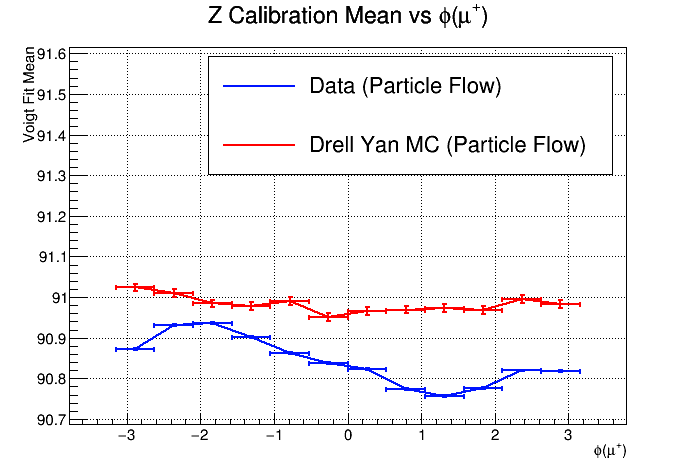
\includegraphics[width=0.32\linewidth]{figures/muon_calib/zcal_pf_mc-data_mean_phi_plus.png}
  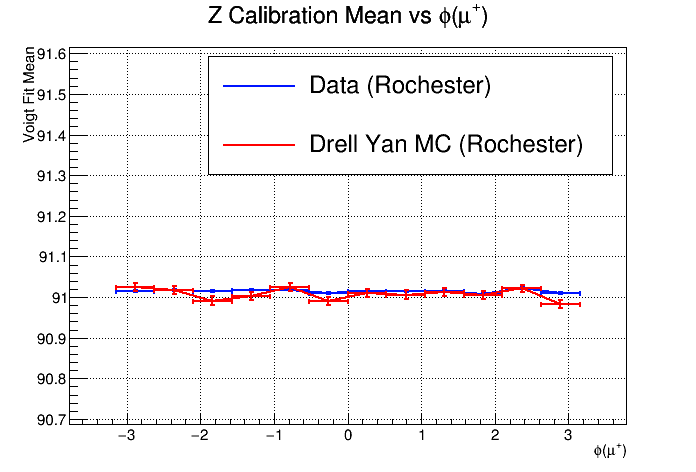
\includegraphics[width=0.32\linewidth]{figures/muon_calib/zcal_roch_mc-data_mean_phi_plus.png}
  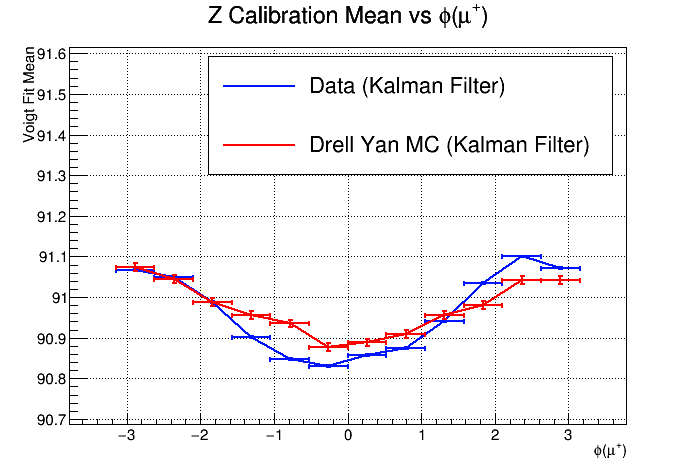
\includegraphics[width=0.32\linewidth]{figures/muon_calib/zcal_kamu_mc-data_mean_phi_plus.png}\\
  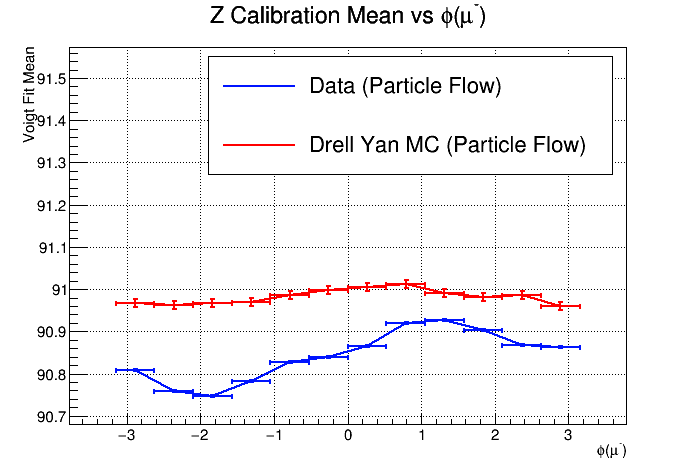
\includegraphics[width=0.32\linewidth]{figures/muon_calib/zcal_pf_mc-data_mean_phi_minus.png}
  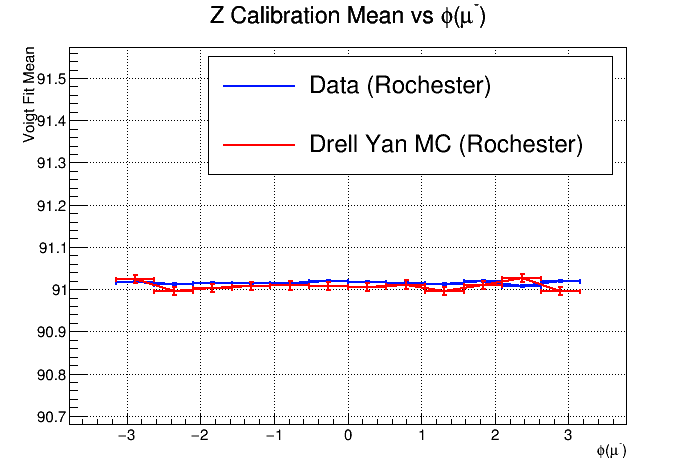
\includegraphics[width=0.32\linewidth]{figures/muon_calib/zcal_roch_mc-data_mean_phi_minus.png}
  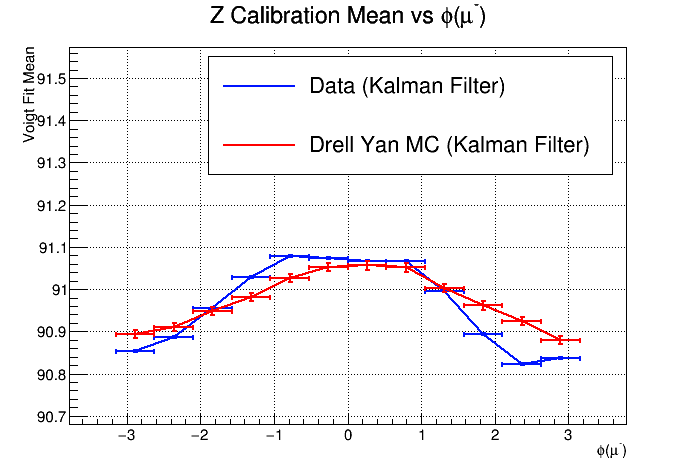
\includegraphics[width=0.32\linewidth]{figures/muon_calib/zcal_kamu_mc-data_mean_phi_minus.png}
  \caption{Comparing Uncorrected (left), Rochester (center) and Kalman (right) Corrections effects on Z Scale.}
  \label{fig:higgs_selections_zscale}
\end{figure}

\begin{figure}[!h]
  \centering
  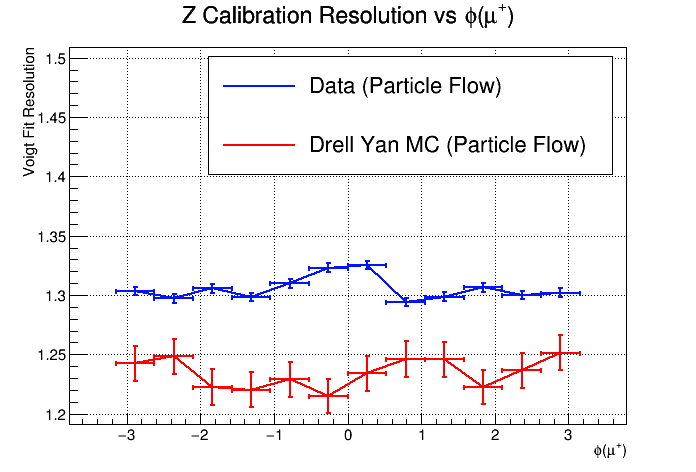
\includegraphics[width=0.32\linewidth]{figures/muon_calib/zcal_pf_mc-data_res_phi_plus.png}
  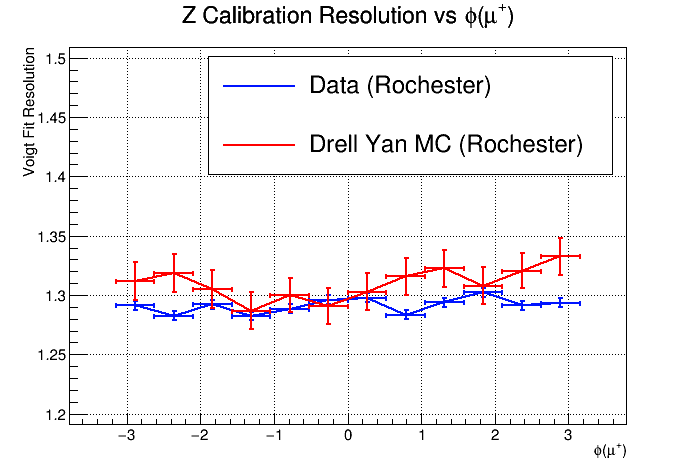
\includegraphics[width=0.32\linewidth]{figures/muon_calib/zcal_roch_mc-data_res_phi_plus.png}
  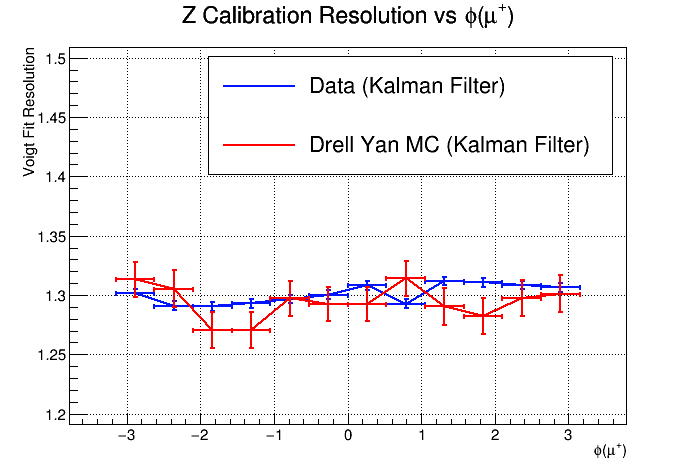
\includegraphics[width=0.32\linewidth]{figures/muon_calib/zcal_kamu_mc-data_res_phi_plus.png}\\
  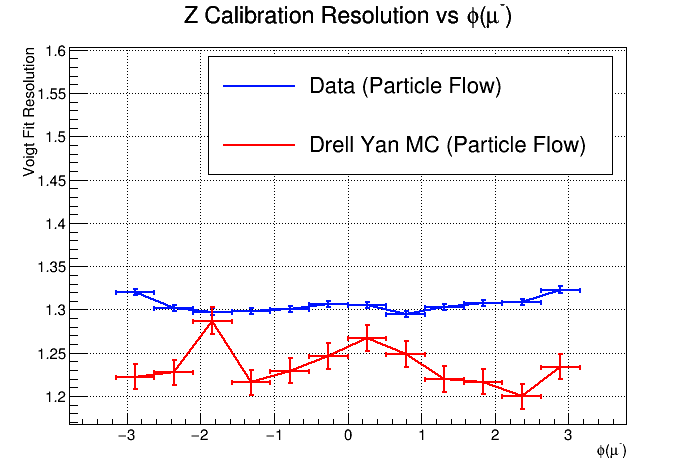
\includegraphics[width=0.32\linewidth]{figures/muon_calib/zcal_pf_mc-data_res_phi_minus.png}
  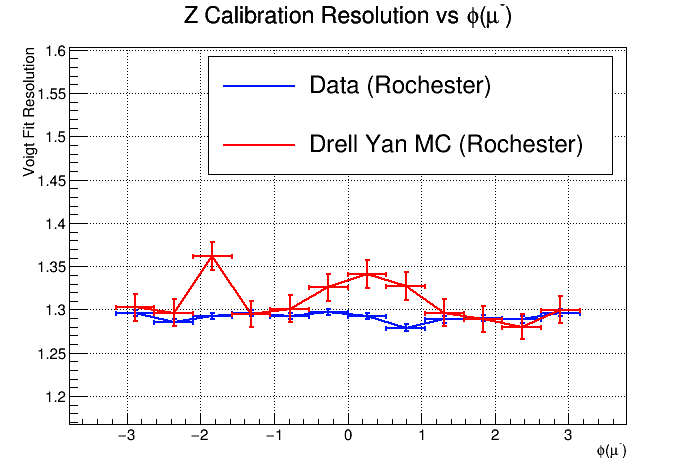
\includegraphics[width=0.32\linewidth]{figures/muon_calib/zcal_roch_mc-data_res_phi_minus.png}
  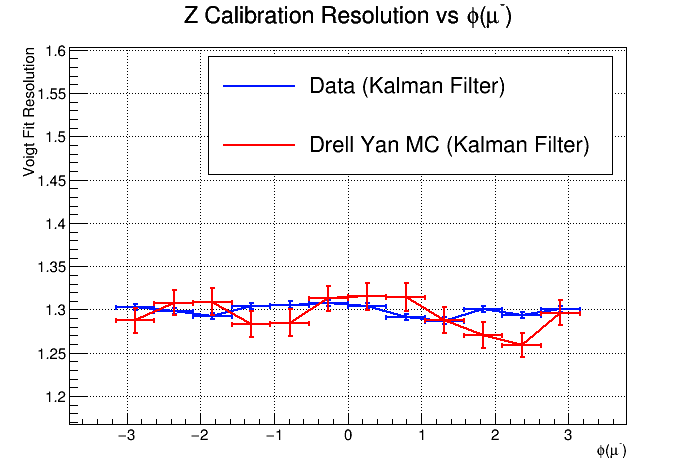
\includegraphics[width=0.32\linewidth]{figures/muon_calib/zcal_kamu_mc-data_res_phi_minus.png}
  \caption{Comparing Uncorrected (left), Rochester (center) and Kalman (right) Corrections effects on Z Resolution.}
  \label{fig:higgs_selections_zresolution}
\end{figure}

\subsection{Jet Selections}
Jets are reconstructed from PF candidates with the anti-$\kappa_{T}$ algorithm~\cite{Cacciari:2008gp} with a distance parameter of 0.4 after rejecting the charged hadrons that are associated to pileup primary vertices. Jets are cleaned against muons - jets overlapping with the selected PF muons, $\Delta R < 0.4$, are not considered further in the analysis. The selected jets with a minimum \pt of 30 GeV and a maximum $|\eta|$ of 4.7 are corrected in energy in order to account for the non-uniform detector response.

The PF jets are further required to fulfill the jet identification criteria.
Candidates with $|\eta|$ less than 2.7 are required to contain at
least one charged PF candidate and have a non-zero charged energy fraction,
and a charged electromagnetic energy fraction less than 0.99. The
neutral and photon energy fraction must be less than 0.99. Jets in
the region $2.7<|\eta|<3.0$ are required to have a neutral electromagnetic
fraction of greater than 0.01 and neutral hadron fraction less than
0.98 while jets with pseudorapidity above 3.0 are required to have more
than 10 neutral particles and a neutral electromagnetic energy fraction
less than 0.9.

For reconstructed jets with $|\eta| < 2.4$, the combined secondary vertex b-tagging algorithm (CSVv2)~\cite{Chatrchyan:2012jua} response is used to discriminate against the $t\bar{t}$ background process events when defining the event categories. The CSVv2 medium operating point is chosen as base line for this analysis and corresponds to a b-tagging efficiency of $60-65\%$ while the misidentification rate for light quarks such as $u$, $d$, $s$, and gluon jets is approximately 1\%.

\subsection{HLT Selections}
Our search requires one of the following Single Isolated Muon Triggers to fire per event:
\begin{itemize}
  \item HLT\_IsoMu24
  \item HLT\_IsoTkMu24
\end{itemize}
The choice of the threshold is driven by the requirement of the lowest \pt threshold to be present during the whole course of datataking. These triggers require the event to have at least one isolated muon candidate with \pt above 24 GeV, with no explicit restriction on its pseudorapidity.

\subsection{Primary Vertex Selection}
One of the top requirements on selecting a proton-proton collision event is the presence of at least 1 valid Primary Vertex with the following conditions:
\begin{itemize}
  \item $ndf \ge 4$ - number of tracks originating from this PV is greater than 4
  \item $\rho < 2$ cm and $|Z| < 24$ cm - displacement along either Z-axis or in the transverse plan should be minimal w.r.t. Interaction Point, defined as (0,0,0).
\end{itemize}

\subsection{Selections Summary}
We can summarize cuts and selections for our search as follows:
\begin{itemize}
  \item At least 1 Primary Vertex passing the PV Selections
  \item At least 1 of the HLT Paths fired
  \item At least 2 opposite sign muons which pass Muon Selections. If more than 1 pair - choose the 2 candidates with the highest \pt. That is the Higgs Candidate.
  \item At least 1 muon from the Higgs Candidate pair with $p_t > 26$ GeV and is matched to the HLT Path that fires the event with $\Delta R < 0.1$.
  \item Filter out the jets that do not pass the Jet Selections, but do not require a certain number of them at this stage.
\end{itemize}

\subsection{Validation}
After applying all of the specified selections, we arrive at a set of events that we are going to further use in order to maximize the sensitivity of our search. However, before proceeding to the next section, we need to validate basic kinematic variables for the inclusive distributions.

First, in the figure~\ref{fig:higgs_selections_inclusivemassnocorr}, inclusive dimuon mass distribution is presented without any muon momentum corrections applied. Notice the presence of a kick near the Z peak. It is the result of a discrepancy in both the mass scale and resolution.
\begin{figure}[!h]
  \centering
  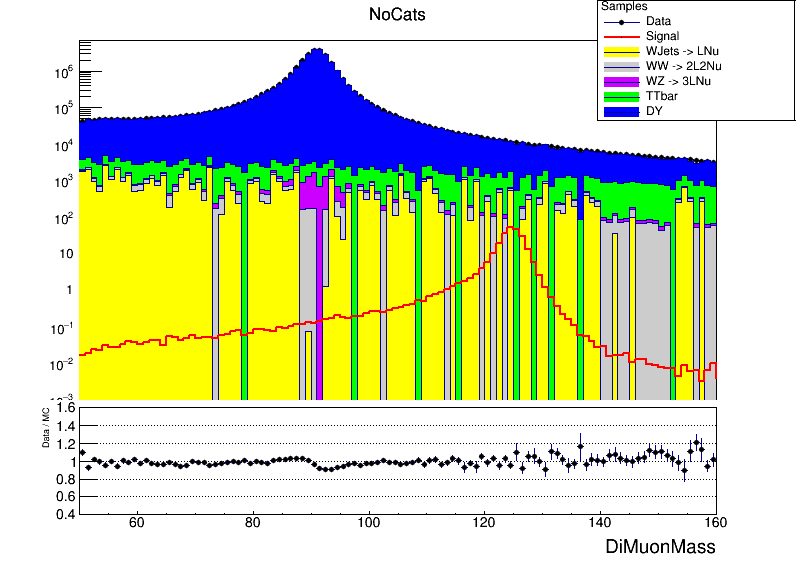
\includegraphics[width=0.5\linewidth]{figures/ch_higgs/distributions/baseline_nocorrections/distribution__NoCats__DiMuonMass__logY.png}
  \caption{Inclusive Dimuon Mass Distributions without any Muon Corrections. Notice the discrepancy around the Z peak}
  \label{fig:higgs_selections_inclusivemassnocorr}
\end{figure}

Second, in the figure~\ref{fig:higgs_selections_inclusivekinematic}, distributions of various kinematic variables after passing the selections are presented.
\begin{figure}[!h]
  \centering
  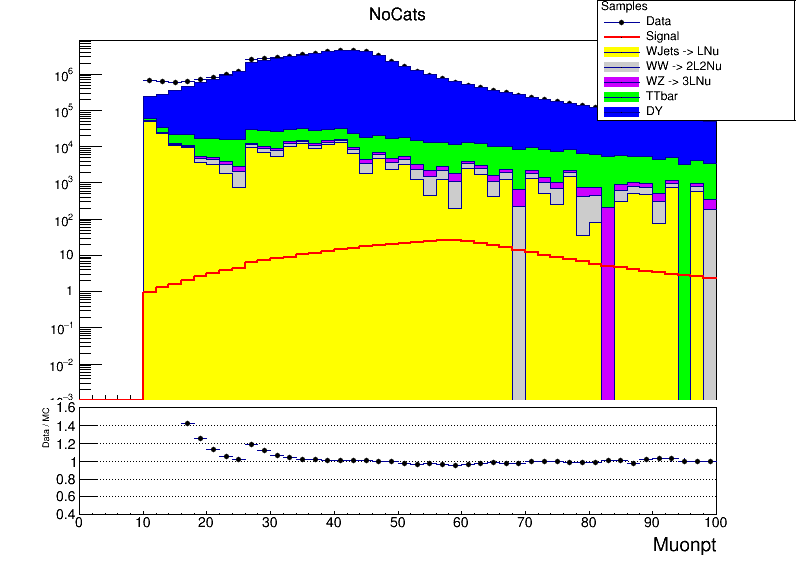
\includegraphics[width=0.45\linewidth]{figures/ch_higgs/distributions/baseline_kalman/distribution__NoCats__Muonpt__logY.png}
  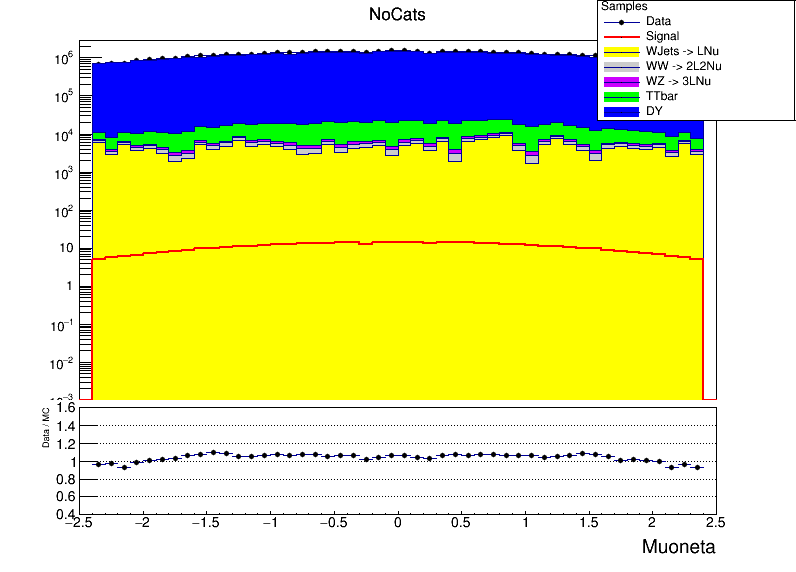
\includegraphics[width=0.45\linewidth]{figures/ch_higgs/distributions/baseline_kalman/distribution__NoCats__Muoneta__logY.png}\\
  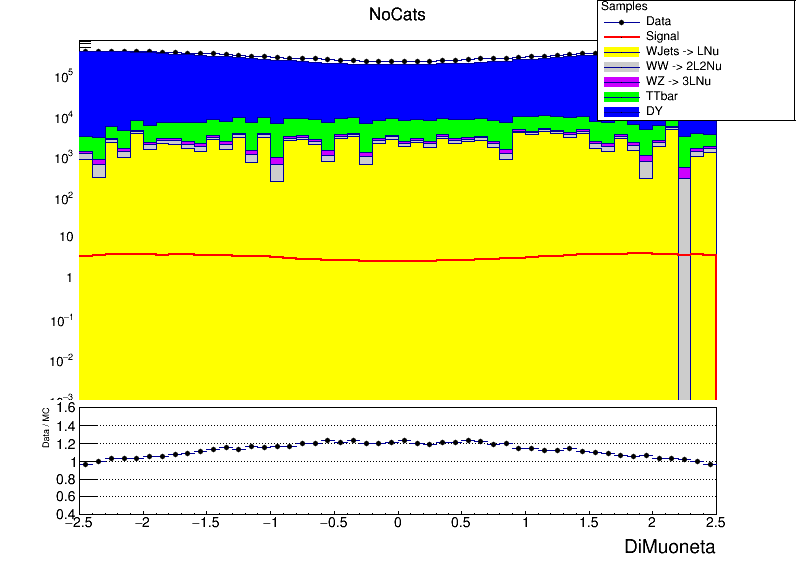
\includegraphics[width=0.45\linewidth]{figures/ch_higgs/distributions/baseline_kalman/distribution__NoCats__DiMuoneta__logY.png}
  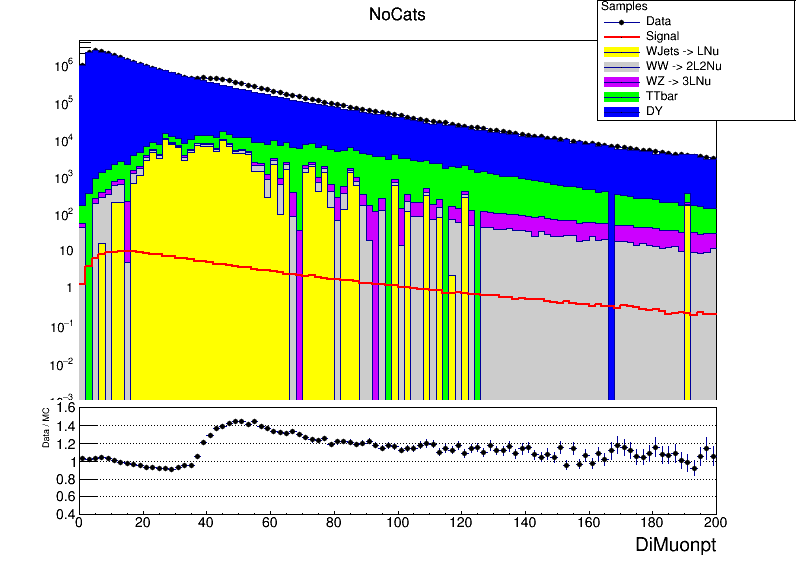
\includegraphics[width=0.45\linewidth]{figures/ch_higgs/distributions/baseline_kalman/distribution__NoCats__DiMuonpt__logY.png}
  \caption{Inclusive Kinematic Distributions.}
  \label{fig:higgs_selections_inclusivekinematic}
\end{figure}

Furthermore, in the figure~\ref{fig:higgs_selections_inclusivemass}, the inclusive dimuon mass distributions are shown with Rochester and Kalman corrections respectively applied to both Data and Monte Carlo. Notice that the discrepancy in scale and resolution is not present anymore around the Z peak.
\begin{figure}[hbp]
  \centering
  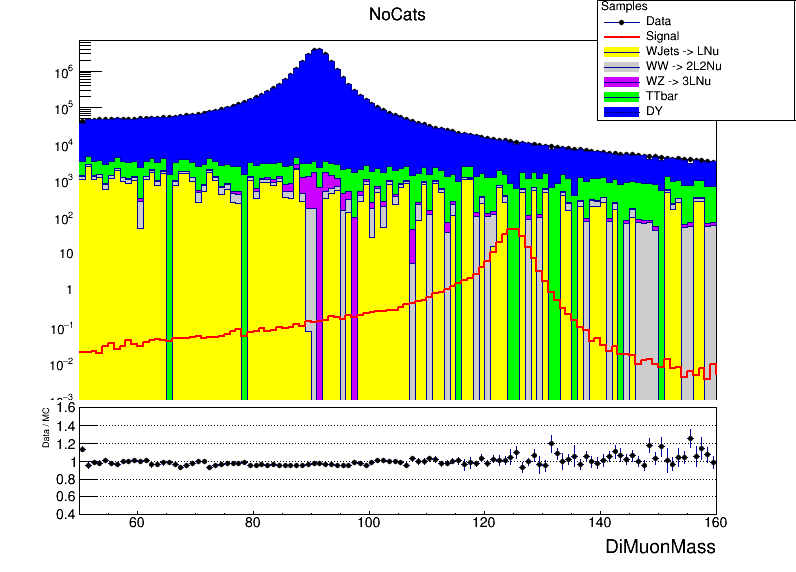
\includegraphics[width=0.9\linewidth]{figures/ch_higgs/distributions/baseline_rochester/distribution__NoCats__DiMuonMass__logY.png}\\
  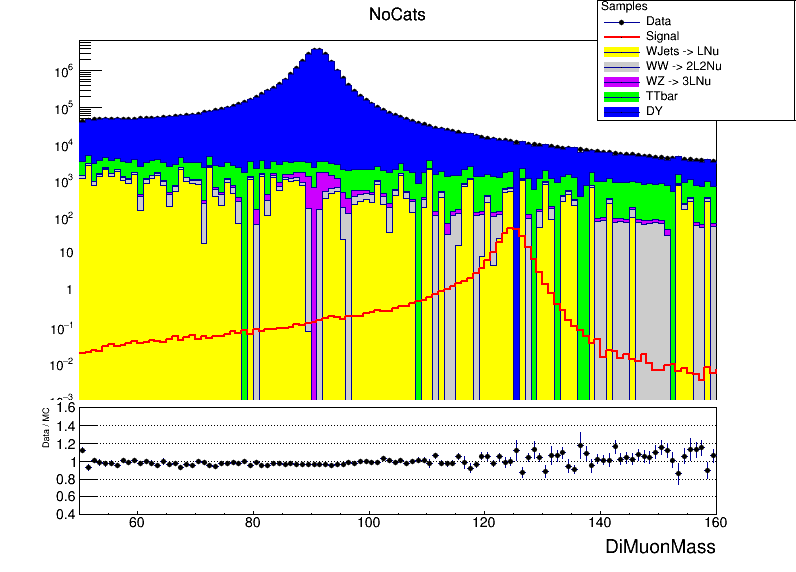
\includegraphics[width=0.9\linewidth]{figures/ch_higgs/distributions/baseline_kalman/distribution__NoCats__DiMuonMass__logY.png}
  \caption{Inclusive Dimuon Mass Distributions. Rochester (Left) and Kalman (Right) Corrections applied}
  \label{fig:higgs_selections_inclusivemass}
\end{figure}



% \subsection{Object validation}
% After applying all the selection cuts and scale factors, we validate the MC simulation
% on data events where the candidate muon pair has an invariant mass greater than 60~GeV.

% \begin{figure}[hbp]
%   \centering
%   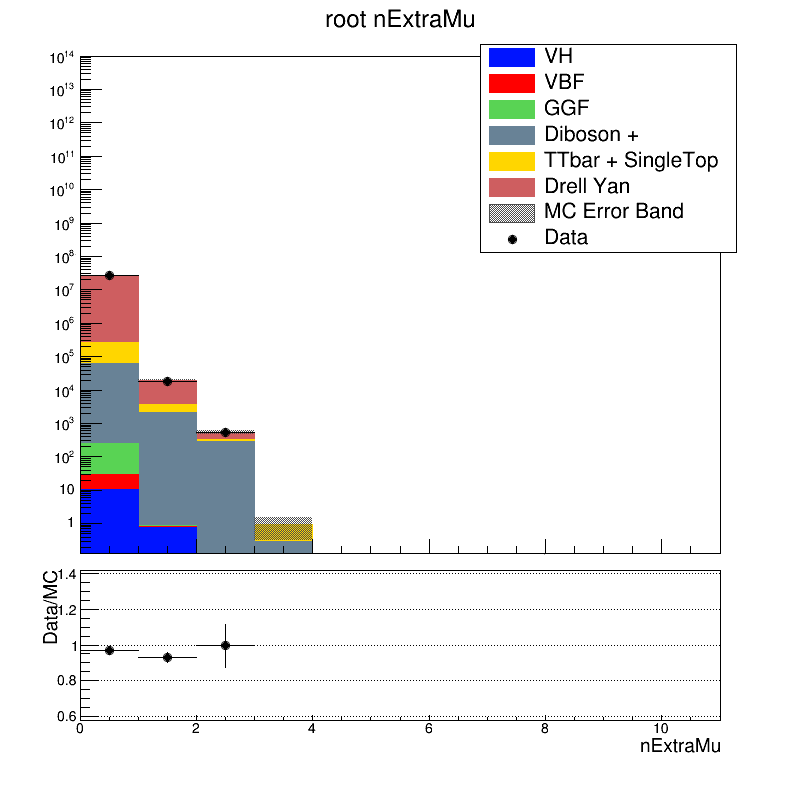
\includegraphics[width=0.32\linewidth]{figures/event_sel/nExtraMu_root.png}
%   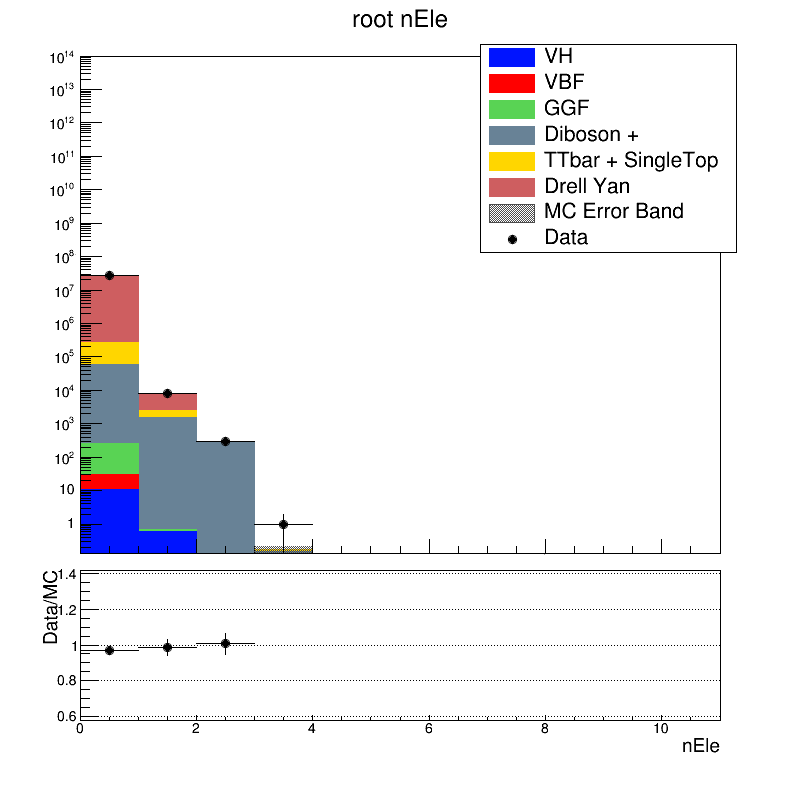
\includegraphics[width=0.32\linewidth]{figures/event_sel/nEle_root.png}
%   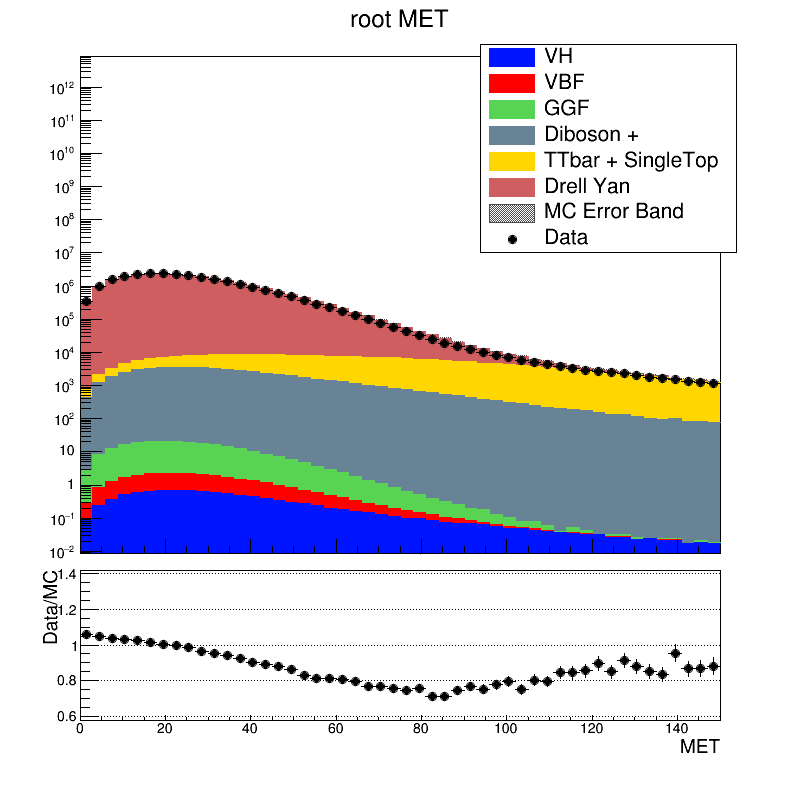
\includegraphics[width=0.32\linewidth]{figures/event_sel/MET_root.png}
%   \caption
%    {Validation of global event variables.}
%   \label{fig:valid_evt}
% \end{figure}

% \begin{figure}[hbp]
%   \centering
%   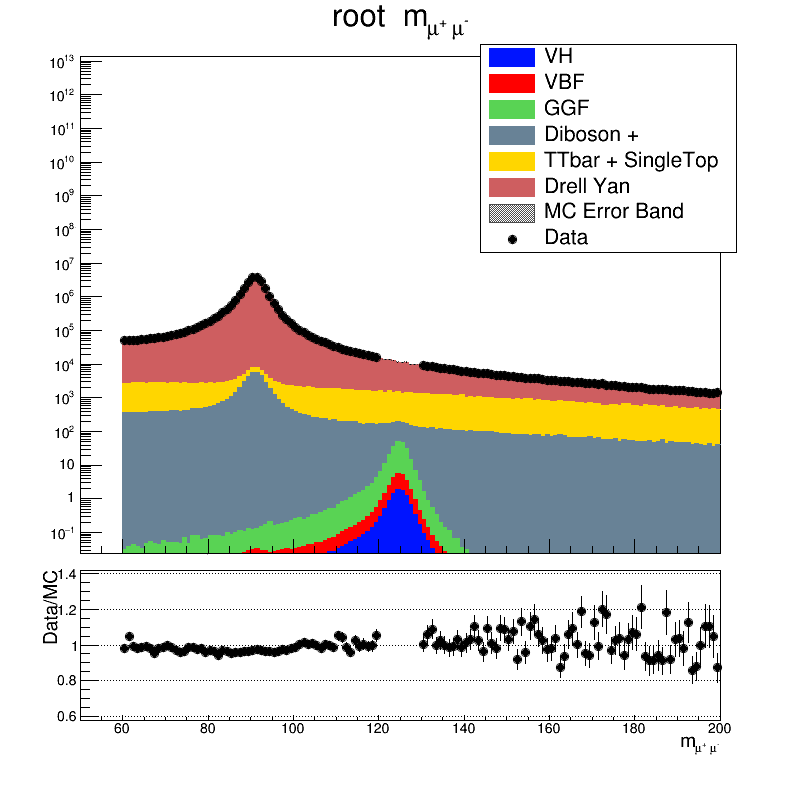
\includegraphics[width=0.32\linewidth]{figures/event_sel/dimu_mass_Roch_root.png}
%   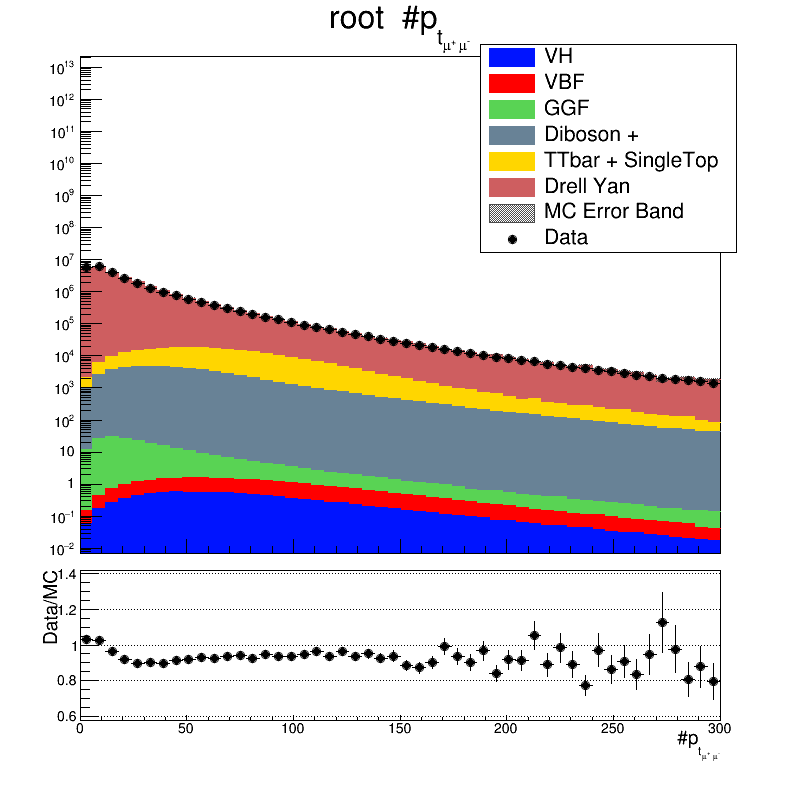
\includegraphics[width=0.32\linewidth]{figures/event_sel/dimu_pt_root.png}
%   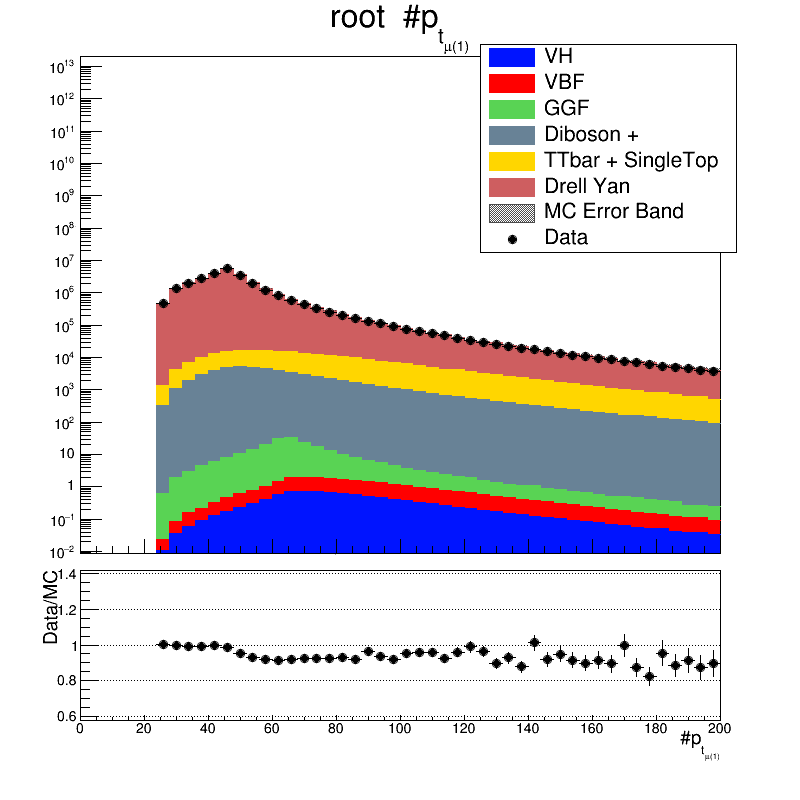
\includegraphics[width=0.32\linewidth]{figures/event_sel/mu1_pt_root.png}
%   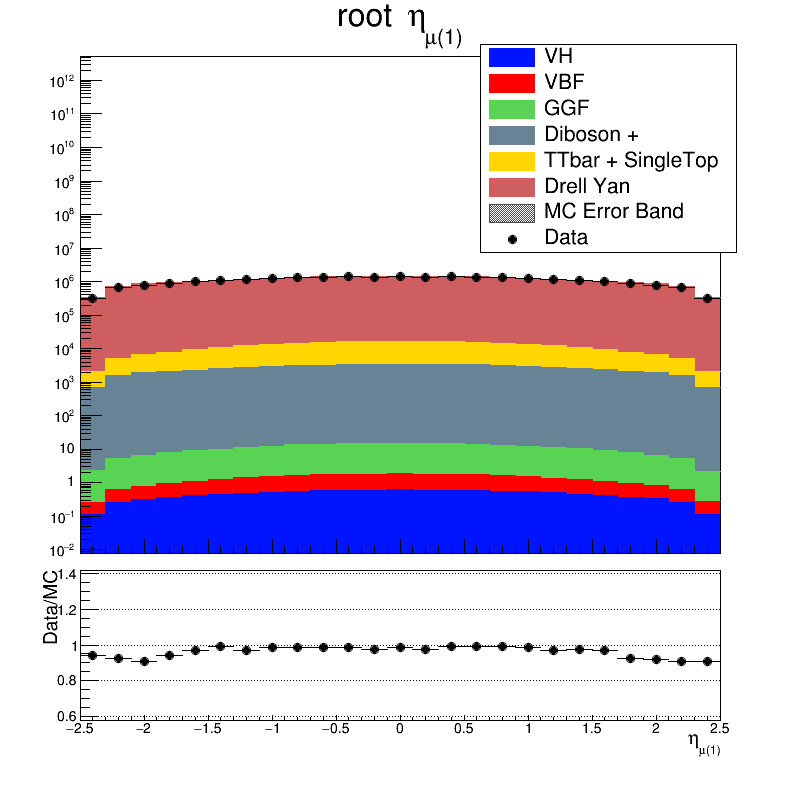
\includegraphics[width=0.32\linewidth]{figures/event_sel/mu1_eta_root.png}
%   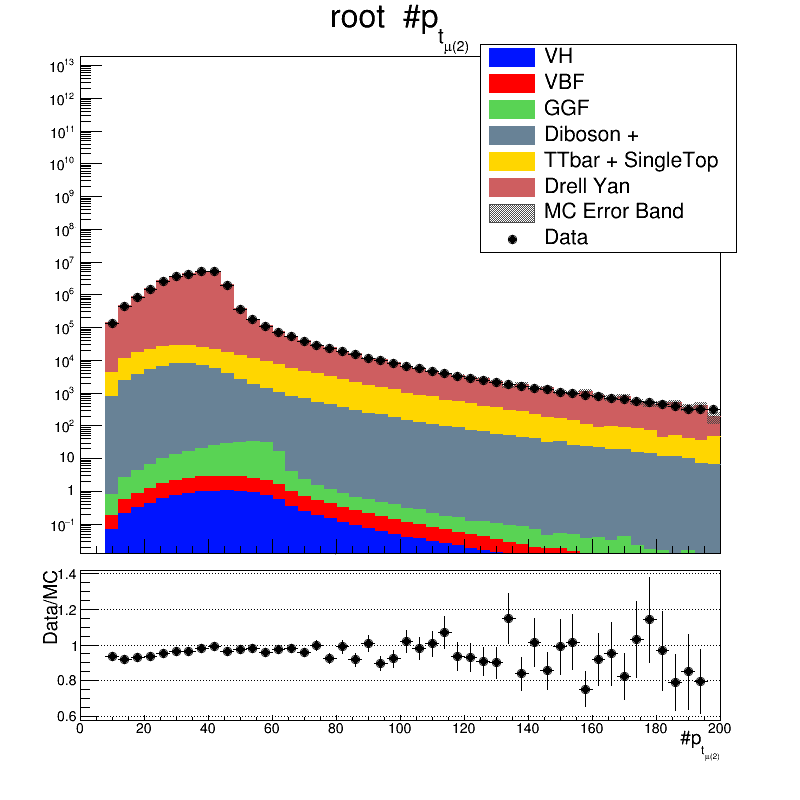
\includegraphics[width=0.32\linewidth]{figures/event_sel/mu2_pt_root.png}
%   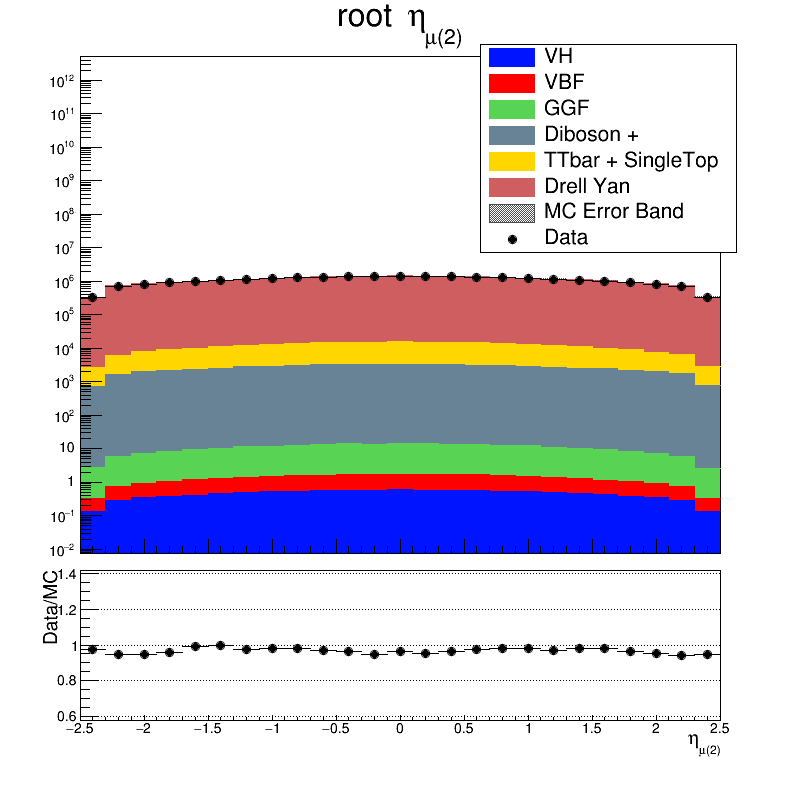
\includegraphics[width=0.32\linewidth]{figures/event_sel/mu2_eta_root.png}
%   \caption
%    {Validation of muon-related variables.}
%   \label{fig:valid_muons}
% \end{figure}

% \begin{figure}[hbp]
%   \centering
%   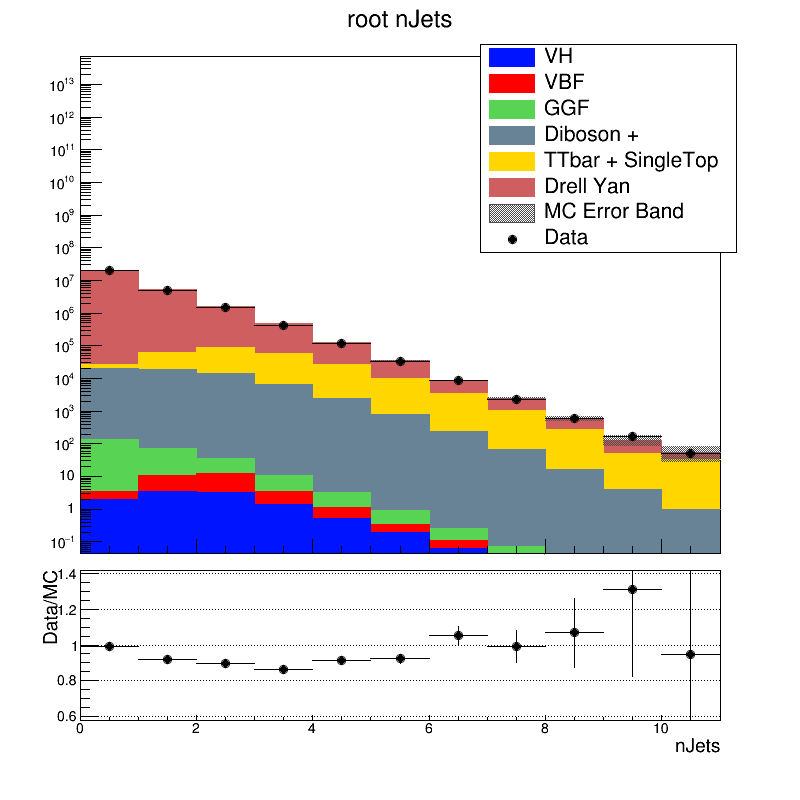
\includegraphics[width=0.32\linewidth]{figures/event_sel/nJets_root.png}
%   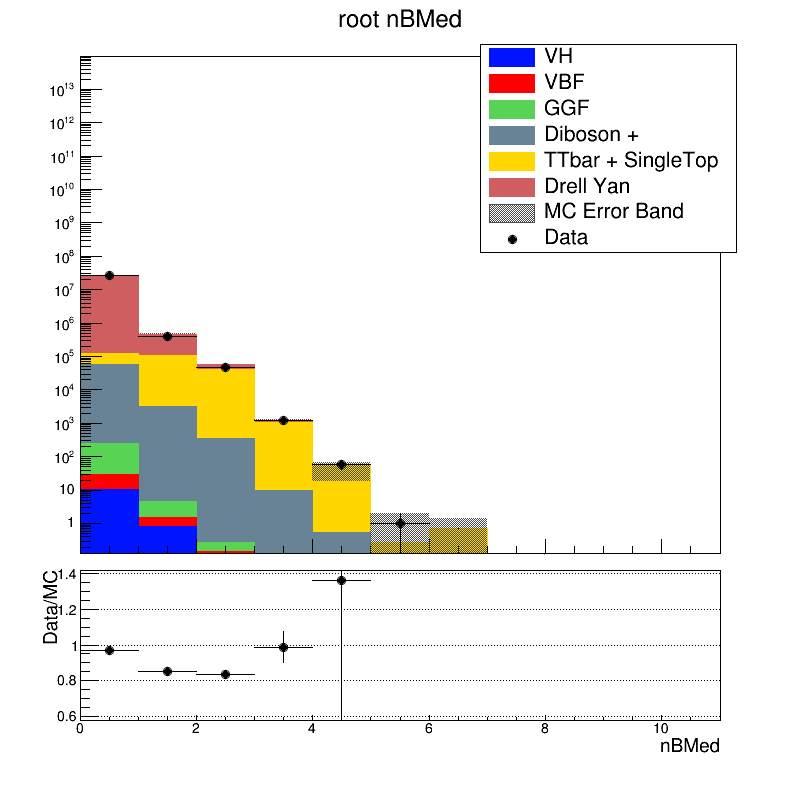
\includegraphics[width=0.32\linewidth]{figures/event_sel/nBMed_root.png}
%   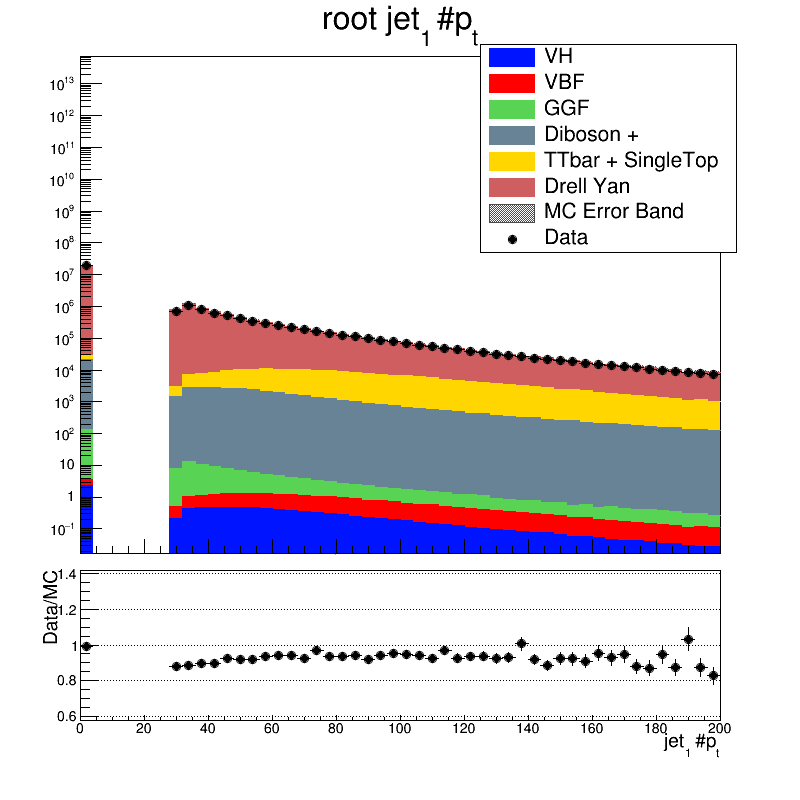
\includegraphics[width=0.32\linewidth]{figures/event_sel/jet1_pt_root.png}
%   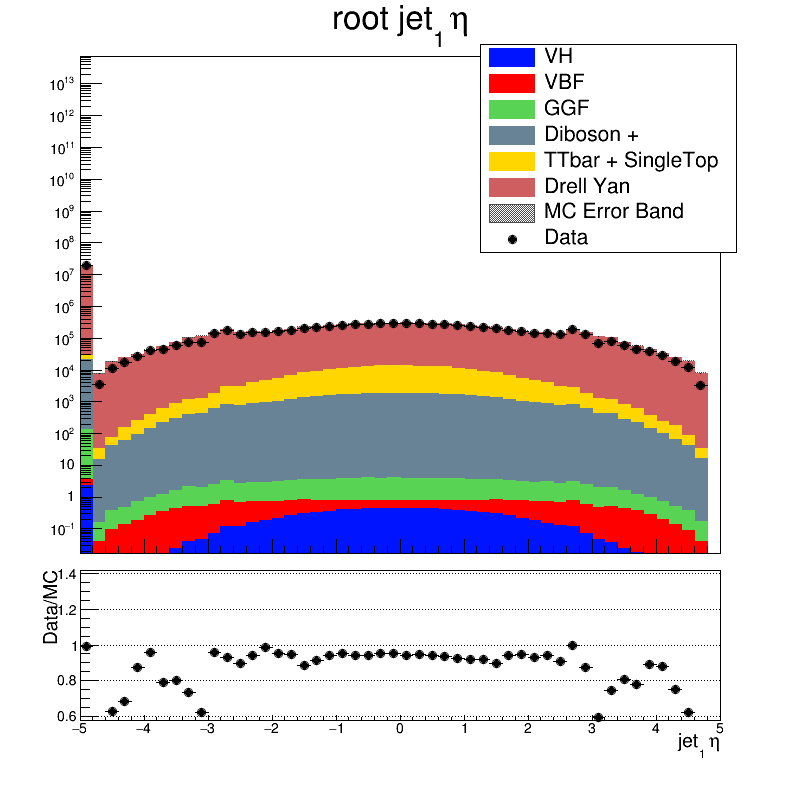
\includegraphics[width=0.32\linewidth]{figures/event_sel/jet1_eta_root.png}
%   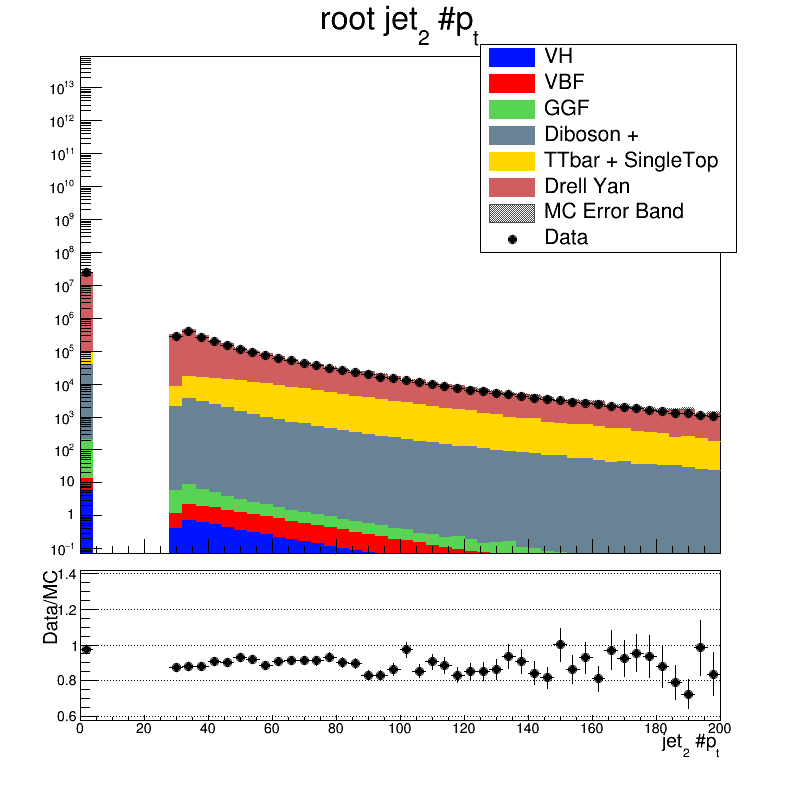
\includegraphics[width=0.32\linewidth]{figures/event_sel/jet2_pt_root.png}
%   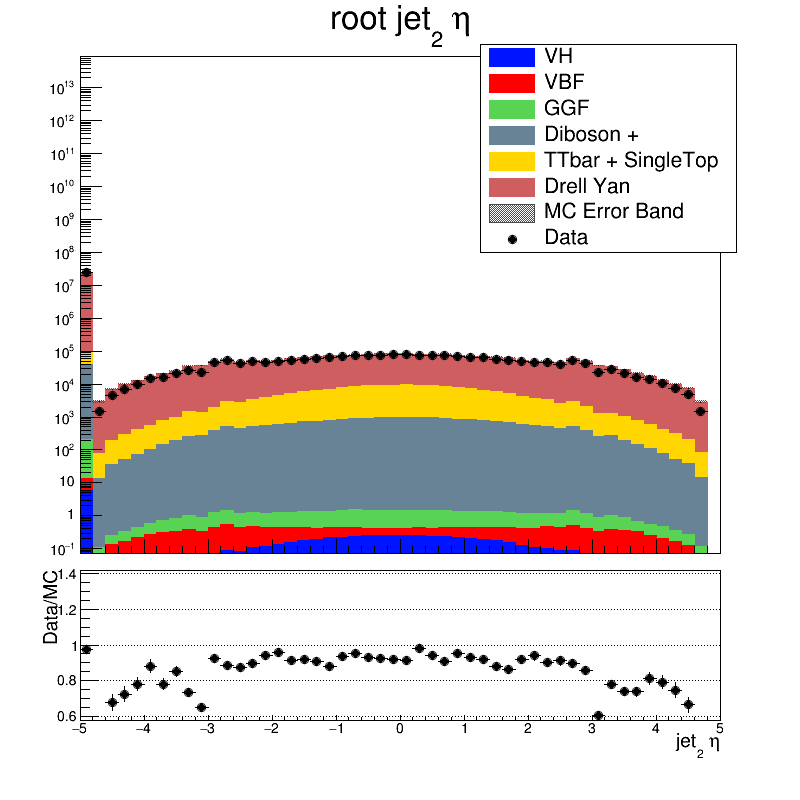
\includegraphics[width=0.32\linewidth]{figures/event_sel/jet2_eta_root.png}
%   \caption
%    {Validation of jet-related variables.}
%   \label{fig:valid_jets}
% \end{figure}




\section{Event Categorization}\label{section:higgs_categorization}
For the purpose of increasing the sensitivity of our analysis, the next step performed is the categorization of events into different subclasses. The basic idea is that we want to utilize the knowledge about two important characteristics of our search: the physics of interest, differences between the production processes, and the fact that our muon detectors intrinsically have better resolution for certain geometrical regions (barrel vs endcap). Using this information will allow us to substantially increase the significance of the Standard Model signal over the expected background.

\subsection{Baseline Categorization}
During the CMS Run I analysis campaign, the categorization procedure used was optimized to separate VBF like events from the rest by requiring the presence of at least 2 jets, pssing the Jet Selections, and going into the opposite ends of our detector and employing large Missing Transverse Energy (MET) selection. Moreover, the resolution of Muon System is significantly better in the Barrel region than in the Endcap, therefore we subdivide the space in $\eta$ variable by defining:
\begin{itemize}
  \item Barrel: $|\eta| < 0.8$
  \item Overlap: $|\eta| \ge 0.8$ \& $|\eta| < 1.6$
  \item Endcap: $|\eta| \ge 1.6$ \& $|\eta| < 2.1$
\end{itemize}
Furthermore, once we have a Higgs candidate pair, we tag each muon based on the region of the detector it was reconstructed in based on its $\eta$. The exact selections applied in the baseline categorization procedure follow:
\begin{itemize}
  \item $njets \ge 2$ \& $p_{t}^{j1} > 40$ GeV \& $p_{t}^{MET} < 40$ GeV - require at least 2 jets with thresholds on \pt of the leading jet and Missing Energy Transverse.
    \begin{itemize}
      \item VBFTight Category: $m_{jj} > 650$ GeV \& $|\Delta \eta| > 3.5$ - category targeting the Vector Boson Fusion production mechanism. The signature is the presence of 2 jets with a large invariant mass and going into opposite ends of CMS.
      \item GFTight Category: if not VBFTight \& $m_{jj} > 250$ GeV \& $p_{t}^{\mu\mu} > 50$ GeV. In this category, we target Gluon Fusion production together with what does not pass the VBF-like selections.
      \item GFLoose Category: here collect everything that does not pass the VBFTight and GFTight selections.
    \end{itemize}
  \item $njets \le 1$ - the biggest portion of the events will have only 1 or 0 jets total per event (that pass previously discussed selections).
    \begin{itemize}
      \item 01JetsTight Category - $p_t^{\mu\mu} \ge 25$ GeV. The only discriminating variable we are left with at this point is the \pt of the dimuon system that typically has higher values for the signal events.
        \begin{itemize}
          \item 01JetsTightBB: $\mu_{1,2}$ are Barrel
          \item 01JetsTightBE: $\mu_{1}$ is Barrel \& $\mu_2$ is Endcap
          \item 01JetsTightBO: $\mu_{1}$ is Barrel \& $\mu_2$ is Overlap
          \item 01JetsTightEE: $\mu_{1}$ is Endcap \& $\mu_2$ is Endcap
          \item 01JetsTightEO: $\mu_{1}$ is Endcap \& $\mu_2$ is Overlap
          \item 01JetsTightOO: $\mu_{1}$ is Overlap \& $\mu_2$ is Overlap
        \end{itemize}
      \item 01JetsLoose Category - Left over events fall into this category.
        \begin{itemize}
          \item 01JetsLooseBB: $\mu_{1,2}$ are Barrel
          \item 01JetsLooseBE: $\mu_{1}$ is Barrel \& $\mu_2$ is Endcap
          \item 01JetsLooseBO: $\mu_{1}$ is Barrel \& $\mu_2$ is Overlap
          \item 01JetsLooseEE: $\mu_{1}$ is Endcap \& $\mu_2$ is Endcap
          \item 01JetsLooseEO: $\mu_{1}$ is Endcap \& $\mu_2$ is Overlap
          \item 01JetsLooseOO: $\mu_{1}$ is Overlap \& $\mu_2$ is Overlap
        \end{itemize}
    \end{itemize}
\end{itemize}

Figures~\ref{fig:higgs_categorization_2jetsall}-~\ref{fig:higgs_categorization_01jetslooseeeeooo} show dimuon mass distributions for all of the terminal categories. For the final analysis, given that both Muon Corrections are producing similar results, we utilize Kalman Corrections. Data in all of the categories is modelled well by the included backgrounds.
\begin{figure}[H]
  \centering
  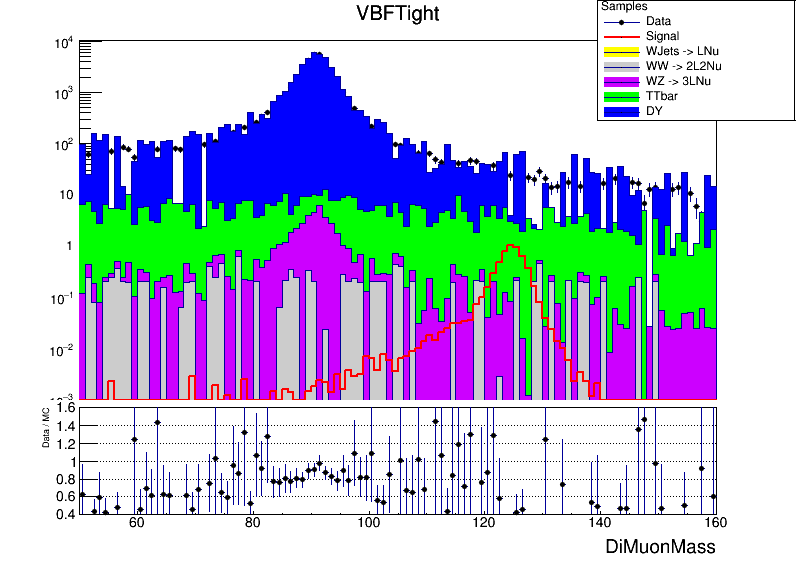
\includegraphics[width=0.65\linewidth]{figures/ch_higgs/distributions/baseline_kalman/distribution__VBFTight__DiMuonMass__logY.png}\\
  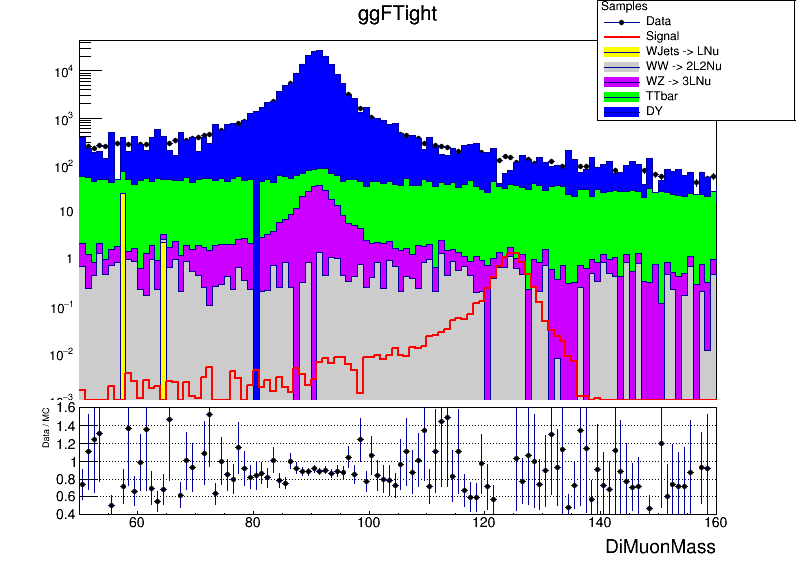
\includegraphics[width=0.65\linewidth]{figures/ch_higgs/distributions/baseline_kalman/distribution__ggFTight__DiMuonMass__logY.png}\\
  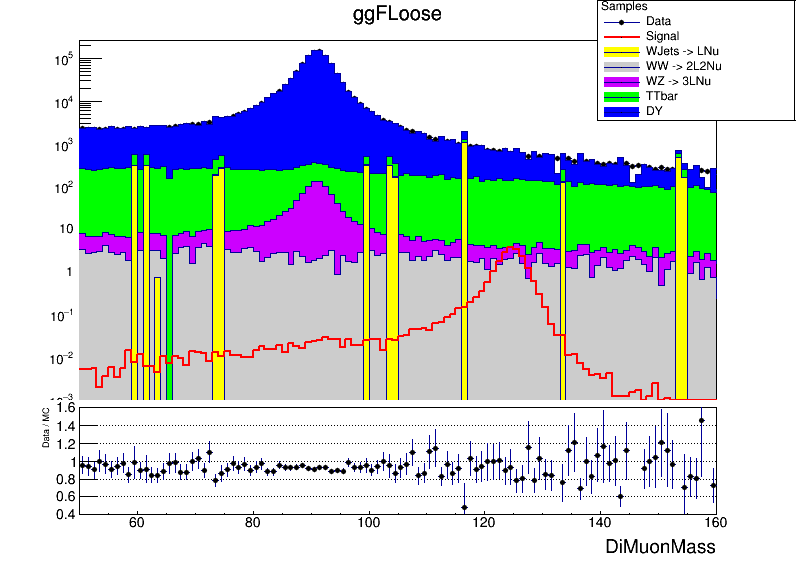
\includegraphics[width=0.65\linewidth]{figures/ch_higgs/distributions/baseline_kalman/distribution__ggFLoose__DiMuonMass__logY.png}
  \caption{Mass Distributions VBFTight (Top), GFTight (Middle) and GFLoose (Bottom) Categories.}
  \label{fig:higgs_categorization_2jetsall}
\end{figure}
\begin{figure}[H]
  \centering
  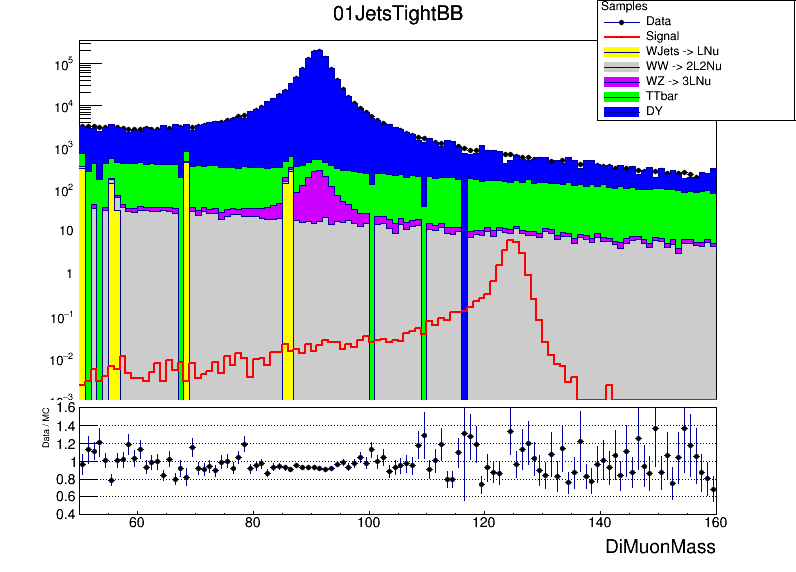
\includegraphics[width=0.65\linewidth]{figures/ch_higgs/distributions/baseline_kalman/distribution__01JetsTightBB__DiMuonMass__logY.png}\\
  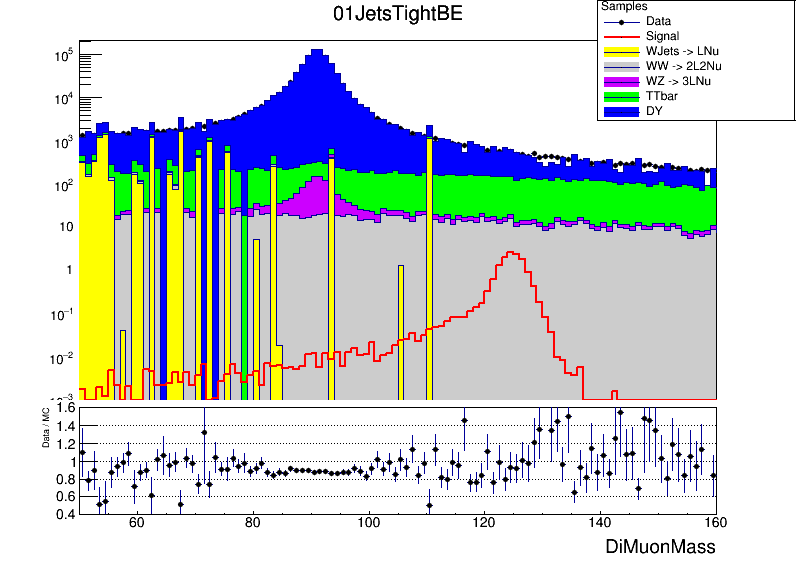
\includegraphics[width=0.65\linewidth]{figures/ch_higgs/distributions/baseline_kalman/distribution__01JetsTightBE__DiMuonMass__logY.png}\\
  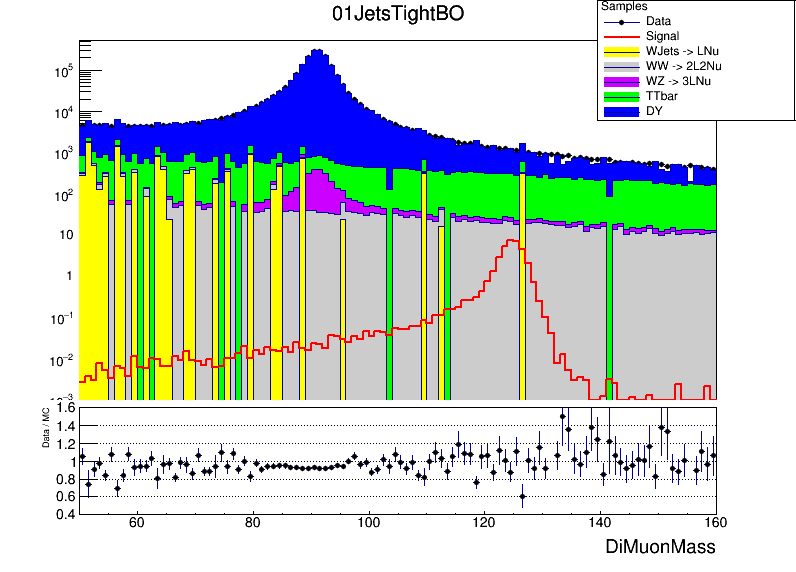
\includegraphics[width=0.65\linewidth]{figures/ch_higgs/distributions/baseline_kalman/distribution__01JetsTightBO__DiMuonMass__logY.png}
  \caption{Mass Distributions 01JetsTightBB (Top), 01JetsTightBE (Middle) and 01JetsTightBO (Bottom) Categories.}
  \label{fig:higgs_categorization_01jetstightbbbebo}
\end{figure}
\begin{figure}[H]
  \centering
  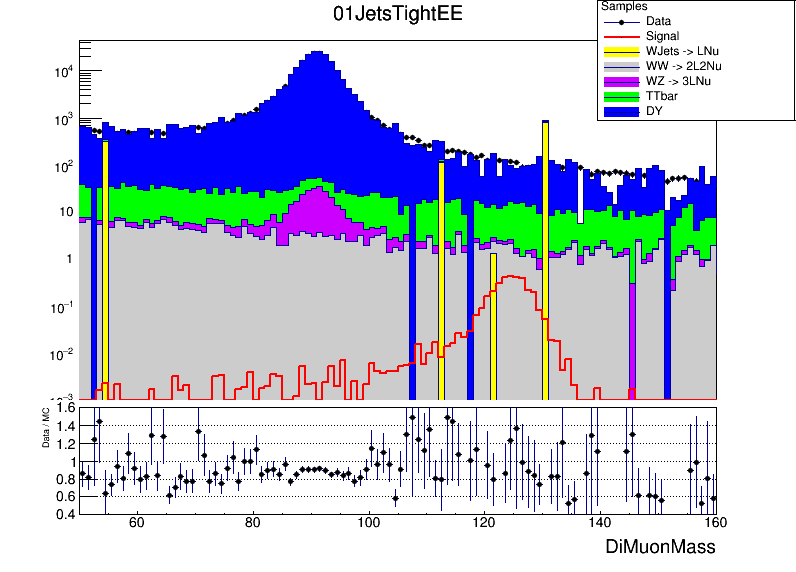
\includegraphics[width=0.65\linewidth]{figures/ch_higgs/distributions/baseline_kalman/distribution__01JetsTightEE__DiMuonMass__logY.png}\\
  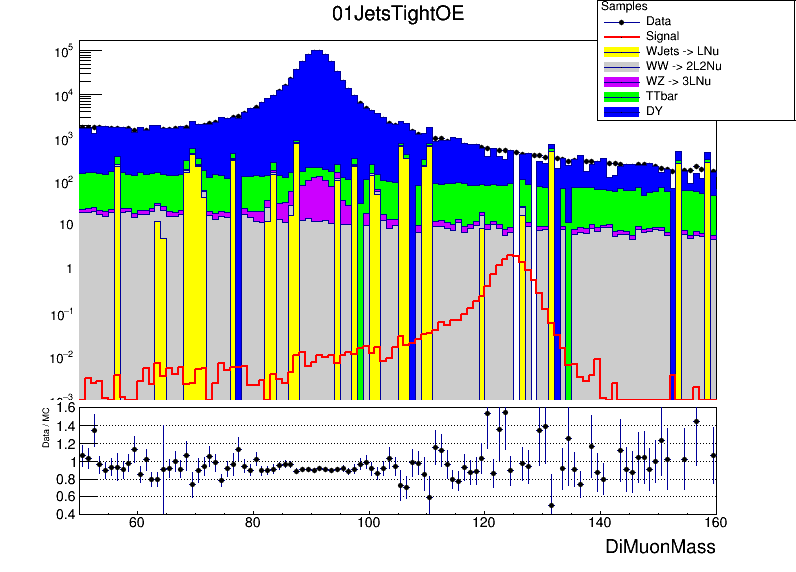
\includegraphics[width=0.65\linewidth]{figures/ch_higgs/distributions/baseline_kalman/distribution__01JetsTightOE__DiMuonMass__logY.png}\\
  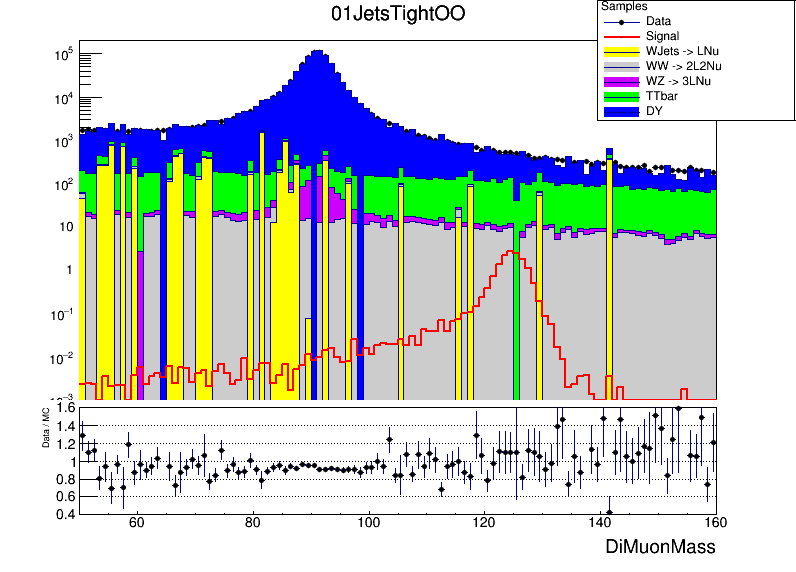
\includegraphics[width=0.65\linewidth]{figures/ch_higgs/distributions/baseline_kalman/distribution__01JetsTightOO__DiMuonMass__logY.png}
  \caption{Mass Distributions 01JetsTightEE (Top), 01JetsTightOE (Middle) and 01JetsTightOO (Bottom) Categories.}
  \label{fig:higgs_categorization_01jetstighteeeooo}
\end{figure}
\begin{figure}[H]
  \centering
  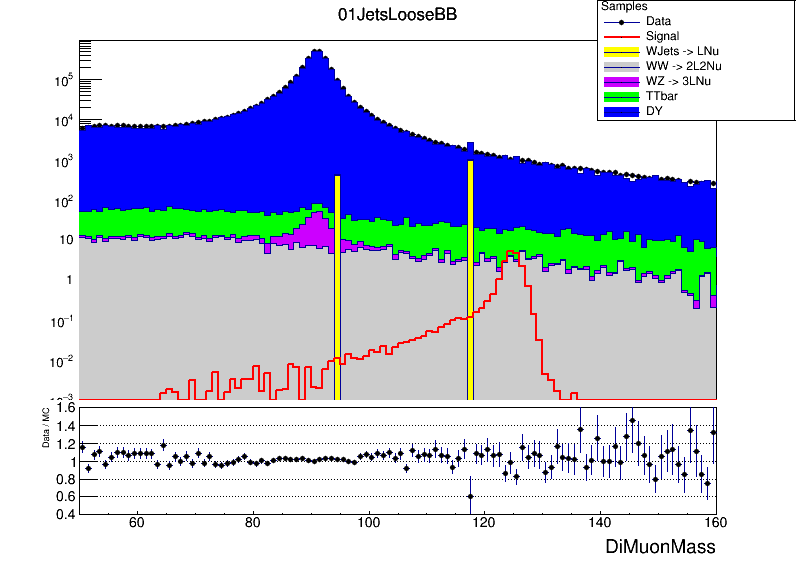
\includegraphics[width=0.65\linewidth]{figures/ch_higgs/distributions/baseline_kalman/distribution__01JetsLooseBB__DiMuonMass__logY.png}\\
  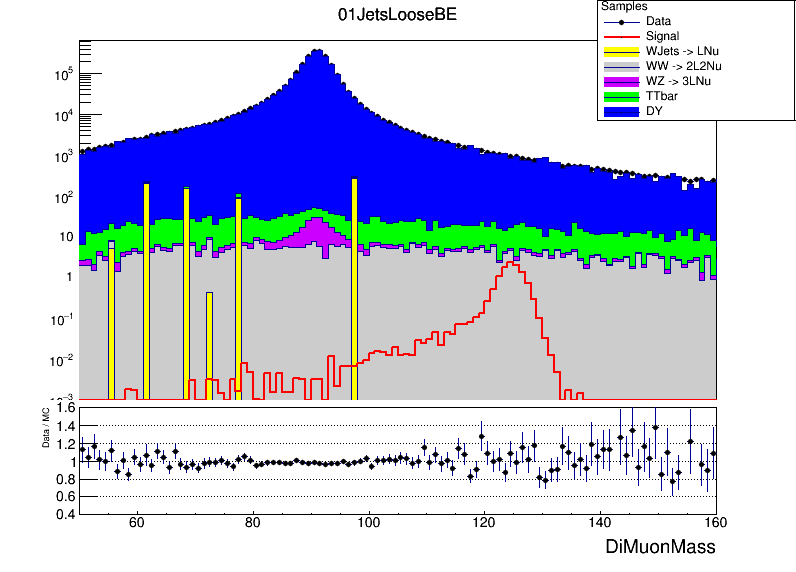
\includegraphics[width=0.65\linewidth]{figures/ch_higgs/distributions/baseline_kalman/distribution__01JetsLooseBE__DiMuonMass__logY.png}\\
  \includegraphics[width=0.65\linewidth]{figures/ch_higgs/distributions/baseline_kalman/distribution__01JetsLooseBO__DiMuonMass__logY.png}
  \caption{Mass Distributions 01JetsLooseBB (Top), 01JetsLooseBE (Middle) and 01JetsLooseBO (Bottom) Categories.}
  \label{fig:higgs_categorization_01jetsloosebbbebo}
\end{figure}
\begin{figure}[H]
  \centering
  \includegraphics[width=0.65\linewidth]{figures/ch_higgs/distributions/baseline_kalman/distribution__01JetsLooseEE__DiMuonMass__logY.png}\\
  \includegraphics[width=0.65\linewidth]{figures/ch_higgs/distributions/baseline_kalman/distribution__01JetsLooseOE__DiMuonMass__logY.png}\\
  \includegraphics[width=0.65\linewidth]{figures/ch_higgs/distributions/baseline_kalman/distribution__01JetsLooseOO__DiMuonMass__logY.png}
  \caption{Mass Distributions 01JetsLooseEE (Top), 01JetsLooseOE (Middle) and 01JetsLooseOO (Bottom) Categories.}
  \label{fig:higgs_categorization_01jetslooseeeeooo}
\end{figure}

\subsection{Greedy Categorization} \label{bdt_training}
Another approach taken was to optimize the manually constructed categorization tree, discussed in the previous section, in a more systematic way by, first, training and applying a Boosted Decision Tree (BDT) for the purpose of signal to background discrimination and, then, using the BDT ouput as a new input feature for optimizing the categorization tree using a greedy optimization procedure.

In the first step, the BDT for the signal to background discrimination has been trained using both signal and background Monte Carlo samples. The BDT implementation from the {\sc ROOT}~\cite{ROOT} framework has been successfully used. Given that background samples are not utilized for the statistical analysis (we use data-driven background treatment discussed further), we employ all of the available MC background events for the purpose of training, cross-validation and testing. However, in terms of the Higgs signal, the even-numbered events are used for the categorization optimization. The rest is reserved for the statistical analysis. The following kinematic variables are used as input features for the BDT:
\begin{itemize}
  \item The $p_t^{\mu\mu}$ of the dimuon system
  \item The $\eta_{\mu\mu}$ of the dimuon system.
  \item The $|\Delta \eta|$ between the muons from the Higgs candidate.
  \item The $|\Delta \phi|$ between the muons from the Higgs candidate.
  \item The $\eta_{jj}$ of the dijet system. 2 highest $p_t$ jets are used.
  \item The $m_{jj}$ of the dijet system. 2 highest $p_t$ jets are used.
  \item The $|\Delta \eta|$ between the 2 highest $p_t$ jets.
  \item The number of Central jets with $|\eta| < 2.4$
  \item The number of Forward jets with $|\eta| > 2.4$
  \item The number of b-tagged jets - jets passing the CSVv2 medium b-tag working point
  \item The \MET
\end{itemize}
As it follows from the above list, there is no dependence on the Higgs candidate mass among the features directly or indirectly. In other words, given the above features, one can not deduce the mass value of the dimuon system. Given that we are performing a search and all of the mass points available will be passed through the same BDT after determining the weights, mass independence is an importan criteria of our discrimination technique.

After the training and cross-validation to tune the hyper parameters of the Decision Tree itself, we run over the test dataset and figure~\ref{fig:higgs_categorization_bdtoutputroc} shows the BDT ouput distributions for both training and testing subsets, which are in a very good agreement. It is a clear sign that we did not overtrain. Furthermore, the ROC curve from figure~\ref{fig:higgs_categorization_bdtoutputroc}, which is an indicator of the efficiency of our selection and rejection at the same time, shows a definite deviation from the diagonal (no discrimination), however even with 100\% inefficiency on background rejection, we still fall short of 100\% of signal rejection. Finally, given that we are not choosing a turning point and not doing a pure binary classficiation, we preserve the BDT score for the next stage.
\begin{figure}[hbp]
  \centering
  \includegraphics[width=0.75\linewidth]{figures/bdt_training/BDT_out_ge0j_all.pdf}\\
  \includegraphics[width=0.75\linewidth]{figures/bdt_training/BDT_ROC_ge0j_all.pdf}
  \caption{BDT score distribution (Top) and Receiver Operating Curve, ROC, (Bottom) - a kind of True Negative/Positive selection efficiency indicator.}
  \label{fig:higgs_categorization_bdtoutputroc}
\end{figure}

The next step of the Greedy Categorization procedure is to optimize the categorization tree selections and perform the actual splitting of events into different subsets. For that purpose, a simple decision tree is used with a custom metric, signal significance, and with the following 2 features:
\begin{itemize}
  \item max($\eta_{\mu_1}$, $\eta_{\mu_2}$) - max $\eta among the muons from the Higgs Candidate pair$
  \item Discriminting BDT score
\end{itemize}
Again, only part of the signal has been used for the training, whereas all of the background events have been passed through the custom decision tree.

Before moving forward with the actual algorithm, we have to provide a few definitions. First of all, we have to acknowledge, that the objects we are going to work with are the dimuon mass histogrammes as in figure~\ref{fig:higgs_categorization_massc0}. For a given mass distribution, we define a Signal Significance ($S_{node}$) according to the equation~\ref{eq:higgs_categorization_significance}. $N^{S}_{c,i}$ and $N^{B}_{c,i}$ are the yields (number of entries) for that particular histogram and for that particular bin. Note that we treat all the bins in the distribution separately and only use those that fall in the [120 GeV, 130 GeV] mass range. Futhermore, the metric, based on which we are going to optimize the splitting, is provided in equation~\ref{eq:higgs_categorization_gain}. Roughly speaking, we use the split that gives us the maximum gain across all the splits that have been tried.
\begin{figure}[hbp]
  \centering
  \includegraphics[width=0.9\linewidth]{figures/ch_higgs/distributions/bdt_uf/distribution__c0__DiMuonMass__logY.png}
  \caption{Mass Distribution for Category ''c0'' - lowest Discriminating BDT score category}
  \label{fig:higgs_categorization_massc0}
\end{figure}
\begin{equation}
  {S^2_c} = \sum_{c,i}N^{S2}_{c,i}/N^{B}_{c,i}
  \label{eq:higgs_categorization_significance}
\end{equation}
\begin{equation}
  {G} = {S^2_{left}} + {S^2_{right}} - {S^2_{node}}
  \label{eq:higgs_categorization_gain}
\end{equation}

After providing all of the important definitions to work with, the actual procedure for the tree splits optimization can be summarized as follows:
\begin{itemize}
  \item Stage 1. Start out with the inclusive set of all events - a node.
  \item Stage 2. Greedily scan through the features and select the split:
    \begin{itemize}
      \item Scan through all of the possible values of max($\eta_{\mu_1}$, $\eta_{\mu_2}$) as split's candidates. Save the split that produces maximum gain.
      \item Scan through all of the possible values of the BDT score. Again, save the split that maximizes the gain for the second feature.
      \item Select the split which maximizes the gain: max(G$_\eta$, G$_{score}$)
    \end{itemize}
  \item Stage n. Repeat Stage 2 recursively for each of the new nodes until the tree reaches the limit on the number of categories or runs out of splitting conditions.
\end{itemize}
The procedure just described is an example of a greedy algorithm, because we do not perform full parameters' phase space optimization as it is computationally infeasible. We greedily optimize the metric of interest step by step iterating over all of the available features.

The outcome of this technique is 13 new categories with the categorization tree shown in figure~\ref{fig:higgs_categorization_bdtcategories}. Integer labels are assigned based on the trained sensitivity of a particular subset, going from the category with the lowest sensitivity, ''c0'', to the one with the highest, ''c12''.
\begin{figure}[hbp]
  \centering
  \includegraphics[width=1.0\linewidth]{figures/bdt_cats/final_categories.png}
  \caption
   {Greedy Categorization Tree.}
  \label{fig:higgs_categorization_bdtcategories}
\end{figure}

\begin{figure}[H]
  \centering
  \includegraphics[width=0.65\linewidth]{figures/ch_higgs/distributions/bdt_uf/distribution__c1__DiMuonMass__logY.png}\\
  \includegraphics[width=0.65\linewidth]{figures/ch_higgs/distributions/bdt_uf/distribution__c2__DiMuonMass__logY.png}\\
  \includegraphics[width=0.65\linewidth]{figures/ch_higgs/distributions/bdt_uf/distribution__c3__DiMuonMass__logY.png}
  \caption{Mass Distributions for c1-c3 subsets from the Greedy Categorization}
  \label{fig:higgs_categorization_greedyc1c3}
\end{figure}
\begin{figure}[H]
  \centering
  \includegraphics[width=0.65\linewidth]{figures/ch_higgs/distributions/bdt_uf/distribution__c4__DiMuonMass__logY.png}\\
  \includegraphics[width=0.65\linewidth]{figures/ch_higgs/distributions/bdt_uf/distribution__c5__DiMuonMass__logY.png}\\
  \includegraphics[width=0.65\linewidth]{figures/ch_higgs/distributions/bdt_uf/distribution__c6__DiMuonMass__logY.png}
  \caption{Msas Distributions for c4-c6 subsets from the Greedy Categorization}
  \label{fig:higgs_categorization_greedyc4c6}
\end{figure}
\begin{figure}[H]
  \centering
  \includegraphics[width=0.65\linewidth]{figures/ch_higgs/distributions/bdt_uf/distribution__c7__DiMuonMass__logY.png}\\
  \includegraphics[width=0.65\linewidth]{figures/ch_higgs/distributions/bdt_uf/distribution__c8__DiMuonMass__logY.png}\\
  \includegraphics[width=0.65\linewidth]{figures/ch_higgs/distributions/bdt_uf/distribution__c9__DiMuonMass__logY.png}
  \caption{Mass Distributions for c7-c9 subsets from the Greedy Categorization}
  \label{fig:higgs_categorization_greedyc7c9}
\end{figure}
\begin{figure}[H]
  \centering
  \includegraphics[width=0.65\linewidth]{figures/ch_higgs/distributions/bdt_uf/distribution__c10__DiMuonMass__logY.png}\\
  \includegraphics[width=0.65\linewidth]{figures/ch_higgs/distributions/bdt_uf/distribution__c11__DiMuonMass__logY.png}\\
  \includegraphics[width=0.65\linewidth]{figures/ch_higgs/distributions/bdt_uf/distribution__c12__DiMuonMass__logY.png}
  \caption{Mass Distributions for c10-c12 subsets fomr the Greedy Categorization}
  \label{fig:higgs_categorization_greedyc10c12}
\end{figure}

Figures~\ref{fig:higgs_categorization_greedyc1c3}-~\ref{fig:higgs_categorization_greedyc10c12} summarize the resulting dimuon mass distributions. The modeling of the dimuon mass agrees well between data and simulations. Furthermore, figures~\ref{fig:higgs_categorization_bdtinput1_inclusive},~\ref{fig:higgs_categorization_bdtinput2_inclusive} provide the comparison of the data with Monte Carlo for the kinematic variables, input features, that are used for the signal discrimination. Figures~\ref{fig:higgs_categorization_bdtinput1_c12},~\ref{fig:higgs_categorization_bdtinput2_c12} show the same features but compared for the most sensitive category. Overall, good agreement between data and simulations is observed, especially for the dimuon mass distribution. Finally, Table~\ref{tab:higgs_categorization_yields} provides a summary on the statistical properties of dimuon mass shapes provided in figures~\ref{fig:higgs_categorization_greedyc1c3}-~\ref{fig:higgs_categorization_greedyc10c12}. One of the important characteristics of our search, although not obvious, is the signal width, provided in terms of Full Width at Half Maximum (FWHM). It is an important feature because the smaller the width is, the more pronounced the signal is, the less influence the shape of the function, used for the background estimation, will have on our Standard Model Higgs signal.
\begin{table}[htb]
  \caption{Comparison of Signal and Background Yields for greedily optimized categories.}
  \label{tab:higgs_categorization_yields}
  \begin{center}
    \begin{tabular}{|c|c|c|c|c|c|}
      \hline
      Category  & Signal FWHM & $N^{S}$ & $N^{B}$ & $\mathrm{N^S / \sqrt{N^B}}$ \\
      \hline
      c0 & 4.4 & 13.4826 & 14187.6 & 0.113193\\
      c1 & 5.8 & 3.52888 & 970.875 & 0.113255\\
      c2 & 5.8 & 14.2112 & 8248.64 & 0.156473\\
      c3 & 6.0 & 3.82012 & 779.594 & 0.136818\\
      c4 & 3.0 & 9.92363 & 1609.08 & 0.24739\\
      c5 & 2.8 & 8.5825  & 1028.08 & 0.267671\\
      c6 & 4.0 & 14.1224 & 2371.09 & 0.290025\\
      c7 & 4.2 & 26.3575 & 6904.16 & 0.317211\\
      c8 & 3.6 & 35.6493 & 11187.4 & 0.337043\\
      c9 & 4.0 & 6.12457 & 451.281 & 0.288305\\
      c10 & 4.0 & 13.9349 & 1667.59 & 0.34124\\
      c11 & 3.0 & 9.59255 & 765.226 & 0.346768\\
      c12 & 4.0 & 9.58541 & 420.983 & 0.467173\\
      \hline
    \end{tabular}
  \end{center}
\end{table}
\begin{figure}[hbp]
  \centering
  \includegraphics[width=0.49\linewidth]{figures/bdt_cats/dimu_eta_root.png}
  \includegraphics[width=0.49\linewidth]{figures/bdt_cats/dimu_abs_dEta_root.png}\\
  \includegraphics[width=0.49\linewidth]{figures/bdt_cats/dimu_abs_dPhi_root.png}
  \includegraphics[width=0.49\linewidth]{figures/bdt_cats/nJetsCent_root.png}
  \caption{Data/MC agreement for the BDT input variables before categorization.}
  \label{fig:higgs_categorization_bdtinput1_inclusive}
\end{figure}

\begin{figure}[hbp]
  \centering
  \includegraphics[width=0.49\linewidth]{figures/bdt_cats/dijet1_mass_root.png}
  \includegraphics[width=0.49\linewidth]{figures/bdt_cats/dijet1_abs_dEta_root.png}\\
  \includegraphics[width=0.49\linewidth]{figures/bdt_cats/dijet2_mass_root.png}
  \includegraphics[width=0.49\linewidth]{figures/bdt_cats/dijet2_abs_dEta_root.png}
  \caption{Data/MC agreement for the BDT input variables before categorization.}
  \label{fig:higgs_categorization_bdtinput2_inclusive}
\end{figure}

\begin{figure}[hbp]
  \centering
  \includegraphics[width=0.49\linewidth]{figures/bdt_cats/dimu_eta_c12.png}
  \includegraphics[width=0.49\linewidth]{figures/bdt_cats/dimu_abs_dEta_c12.png}\\
  \includegraphics[width=0.49\linewidth]{figures/bdt_cats/dimu_abs_dPhi_c12.png}
  \includegraphics[width=0.49\linewidth]{figures/bdt_cats/nJetsCent_c12.png}
  \caption{Data/MC agreement for the BDT input varaibles for the most sensitive category.}
  \label{fig:higgs_categorization_bdtinput1_c12}
\end{figure}

\begin{figure}[hbp]
  \centering
  \includegraphics[width=0.49\linewidth]{figures/bdt_cats/dijet1_mass_c12.png}
  \includegraphics[width=0.49\linewidth]{figures/bdt_cats/dijet1_abs_dEta_c12.png}\\
  \includegraphics[width=0.49\linewidth]{figures/bdt_cats/dijet2_mass_c12.png}
  \includegraphics[width=0.49\linewidth]{figures/bdt_cats/dijet2_abs_dEta_c12.png}
  \caption{Data/MC agreement for the BDT input variables for the most sensitive category.}
  \label{fig:higgs_categorization_bdtinput2_c12}
\end{figure}

% \begin{figure}
%   \includegraphics[width=1.0\linewidth]{figures/bdt_training/BDT_in_ge0j_all.pdf}
%   \includegraphics[width=1.0\linewidth]{figures/bdt_training/BDT_in_ge0j_sep.pdf}
%   \caption{Some BDT input variables for events with $\ge 0$ jets.
%            In the top plots, signal is in blue and background in red.
%            In the bottom plots, the gluon-fusion signal is dark blue, VBF is red, and VH is green,
%            while Drell--Yan and diboson backgrounds are pink, and \ttbar and single top are light blue.}
%   \label{fig:BDT_in_ge0j}
% \end{figure}

% \begin{figure}
%   \includegraphics[width=1.0\linewidth]{figures/bdt_training/BDT_in_le1j_all_A.pdf}
%   \includegraphics[width=1.0\linewidth]{figures/bdt_training/BDT_in_le1j_sep_A.pdf}
%   \caption{Some BDT input variables for events with $\le 1$ jets.
%            In the top plots, signal is in blue and background in red.
%            In the bottom plots, the gluon-fusion signal is dark blue, VBF is red, and VH is green,
%            while Drell--Yan and diboson backgrounds are pink, and \ttbar and single top are light blue.}
%   \label{fig:BDT_in_le1j_A}
% \end{figure}

% \begin{figure}
%   \includegraphics[width=1.0\linewidth]{figures/bdt_training/BDT_in_le1j_all_B.pdf}
%   \includegraphics[width=1.0\linewidth]{figures/bdt_training/BDT_in_le1j_sep_B.pdf}
%   \caption{Some BDT input variables for events with $\le 1$ jets.
%            In the top plots, signal is in blue and background in red.
%            In the bottom plots, the gluon-fusion signal is dark blue, VBF is red, and VH is green,
%            while Drell--Yan and diboson backgrounds are pink, and \ttbar and single top are light blue.}
%   \label{fig:BDT_in_le1j_B}
% \end{figure}

% \begin{figure}
%   \includegraphics[width=1.0\linewidth]{figures/bdt_training/BDT_in_eq2j_sep_B.pdf}
%   \caption{Some BDT input variables for events with $= 2$ jets.
%            The gluon-fusion signal is dark blue, VBF is red, and VH is green,
%            while Drell--Yan and diboson backgrounds are pink, and \ttbar and single top are light blue.}
%   \label{fig:BDT_in_eq2j_B}
% \end{figure}

% \begin{figure}
%   \includegraphics[width=1.0\linewidth]{figures/bdt_training/BDT_in_eq2j_all_A.pdf}
%   \includegraphics[width=1.0\linewidth]{figures/bdt_training/BDT_in_eq2j_sep_A.pdf}
%   \caption{Some BDT input variables for events with $= 2$ jets.
%            In the top plots, signal is in blue and background in red.
%            In the bottom plots, the gluon-fusion signal is dark blue, VBF is red, and VH is green,
%            while Drell--Yan and diboson backgrounds are pink, and \ttbar and single top are light blue.}
%   \label{fig:BDT_in_eq2j_A}
% \end{figure}

% \begin{figure}
%   \includegraphics[width=1.0\linewidth]{figures/bdt_training/BDT_in_ge3j_all_A.pdf}
%   \includegraphics[width=1.0\linewidth]{figures/bdt_training/BDT_in_ge3j_sep_A.pdf}
%   \caption{Some BDT input variables for events with $\ge 3$ jets.
%            In the top plots, signal is in blue and background in red.
%            In the bottom plots, the gluon-fusion signal is dark blue, VBF is red, and VH is green,
%            while Drell--Yan and diboson backgrounds are pink, and \ttbar and single top are light blue.}
%   \label{fig:BDT_in_ge3j_A}
% \end{figure}

% \begin{figure}
%   \includegraphics[width=1.0\linewidth]{figures/bdt_training/BDT_in_ge3j_all_B.pdf}
%   \includegraphics[width=1.0\linewidth]{figures/bdt_training/BDT_in_ge3j_sep_B.pdf}
%   \caption{Some BDT input variables for events with $\ge 3$ jets.
%            In the top plots, signal is in blue and background in red.
%            In the bottom plots, the gluon-fusion signal is dark blue, VBF is red, and VH is green,
%            while Drell--Yan and diboson backgrounds are pink, and \ttbar and single top are light blue.}
%   \label{fig:BDT_in_ge3j_B}
% \end{figure}

% \clearpage

% The BDT output distributions for both the inclusive and $\le 1$, $= 2$, and $\ge 3$
% jet trainings can be seen in Figure~\ref{fig:BDT_out}, with the corresponding ROC curves
% in Figure~\ref{fig:BDT_ROC}.  We also performed a multi-classification which assigned
% separate BDT scores for each of the signal and background classes: ggH, VBF, VH, EWK,
% and TOP.  In the end, the binary signal--background classification algorithm, trained
% on the inclusve $\ge 0$ jets sample of events, provided a signal--background separation
% which was as good as any scheme using either the separate-jet trainings or the
% multi-classification algorithm.

% \begin{figure}
%   \includegraphics[width=0.5\linewidth]{figures/bdt_training/BDT_out_ge0j_all.pdf}
%   \includegraphics[width=0.5\linewidth]{figures/bdt_training/BDT_out_le1j_all.pdf}
%   \includegraphics[width=0.5\linewidth]{figures/bdt_training/BDT_out_eq2j_all.pdf}
%   \includegraphics[width=0.5\linewidth]{figures/bdt_training/BDT_out_ge3j_all.pdf}
%   \caption{The BDT output score for events with $\ge 0$ jets (top left), $\leq 1$ jet (top right),
%            $= 2$ jets (bottom left), and $\ge 3$ jets (bottom right).}
%   \label{fig:BDT_out}
% \end{figure}

% \begin{figure}
%   \includegraphics[width=0.5\linewidth]{figures/bdt_training/BDT_ROC_ge0j_all.pdf}
%   \includegraphics[width=0.5\linewidth]{figures/bdt_training/BDT_ROC_le1j_all.pdf}
%   \includegraphics[width=0.5\linewidth]{figures/bdt_training/BDT_ROC_eq2j_all.pdf}
%   \includegraphics[width=0.5\linewidth]{figures/bdt_training/BDT_ROC_ge3j_all.pdf}
%   \caption{The background-rejection vs. signal efficiency ROC curve from the
%            BDT output score for events with $\ge 0$ jets (top left), $\le 1$ jet (top right),
%            $= 2$ jets (bottom left), and $\ge 3$ jets (bottom right).}
%   \label{fig:BDT_ROC}
% \end{figure}

% \clearpage

% \subsection{BDT for Event Categorization}
% \label{bdt_cats}

% In order to optimize the sensitivity of the \Htomm search in a systematic way, the events
% are categorized based on two criteria: the BDT output score and the muon eta information.
% The output score of the BDT is used to separate signal
% from background events, where the score ranges from -1 (background-like) to +1 (signal-like).
% In addition, the maximum $|\eta|$ value of the two candidate muons is used to isolate events with better
% signal-peak resolution. In order to optimize the choice of BDT and $|\eta|$ cuts, we designed and implemented
% a decision tree autocategorizer to create categories by greedily optimizing a metric corresponding
% to the sensitivity which by proxy minimizes the expected upper limit. The BDT training and the autocategorization
% are performed on 50\% of the signal MC events and 100\% of the background MC events.
% After training the autocategorizer on the signal and background MC to determine the categories,
% the expected limits are calculated using data and the remaining 50\% of simulated signal events. Separating the
% signal into separate training and evaluation sets and excluding the data from the training phase ensure an unbiased estimate for the expected limits.

% \begin{figure}[hbp]
%   \centering
%   \includegraphics[width=0.49\linewidth]{figures/bdt_cats/bdt_score_ggH_VBF_DY_ttbar.pdf}
%   \includegraphics[width=0.49\linewidth]{figures/bdt_cats/bdt_score_inclusive_data_mc.png}
%   \caption
%    {The BDT score on the signal and background Monte Carlo (left), where a higher score marks the signal like events.
%     Note \ttbar on the left as the most distinguishable background and VBF on the right as the most distinguishable signal.
%     The BDT score in data is modeled well by the amc@NLO Drell--Yan MC (right). }
%   \label{fig:bdt_score_inclusive}
% \end{figure}

% \subsection{The Auto-Categorizer}

% In order to account for the resolution, the signal and background events are binned in half-GeV bins in the signal
% region of the dimuon mass spectrum, 120 to 130 GeV. The significance in each bin is then given by $S/\sqrt{B}$.
% The significance for independent bins adds in quadrature, so the net significance is given by

% \begin{equation}
% Net~Significance = \sum_{c,i}S_{c,i}^{2}/B_{c,i}
% \end{equation}

% where $i$ labels the bin in the signal region, and $c$ denotes the category. $S_{c,i}$ is the number of expected signal
% events in the $i^{th}$ bin in that category, and $B_{i,c}$ is the number of expected background events in the $i^{th}$ bin.
% By binning finely enough, the central mass bins contribute the most and the resolution is accounted for.

% \begin{figure}[hbp]
%   \centering
%   \includegraphics[width=0.49\linewidth]{figures/bdt_cats/binning_signal_example.png}
%   \includegraphics[width=0.49\linewidth]{figures/bdt_cats/binning_bg_example.png}
%   \caption
%   {An example of the binned signal and background necessary for the significance metric. The binning keeps the most sensitive bins
%    from being drowned out by the others, providing a measure that accounts for both signal--background discrimination and resolution.}
%   \label{fig:binning_example}
% \end{figure}

% On the first iteration, the autocategorizer calculates the net significance for the set of all events, the inclusive set.
% The algorithm then searches over the inclusive set, checking all possible split values of the maximum muon $|\eta|$. Events
% with maximum $|\eta|$ values less than the split go in one candidate category, and those with eta values greater than or equal
% to the split value go into the other candidate category. For every split candidate, the algorithm calculates the net significance
% in the two categories delineated by the split value. The maximum $|\eta|$ cut value that provides the largest gain in significance
% over the inclusive set is stored. The gain is defined in the equation below where $c1$ and $c2$ are the prospective categories
% created from $c$ by splitting on the feature.

% \begin{equation}
% Gain = \sum_{i}S_{c1,i}^{2}/B_{c1,i} + \sum_{i}S_{c2,i}^{2}/B_{c1,i} - \sum_{i}S_{c,i}^{2}/B_{c,i}
% \end{equation}

% The autocategorizer then searches over the BDT score values and stores the BDT score that provides the largest gain in significance.
% The algorithm chooses to split on either the maximum muon $|\eta|$ or the BDT score (whichever has the higher gain), creating two
% categories from the inclusive set of events. At the next iteration, the autocategorizer repeats the procedure for the two new
% categories and chooses to split the category that provides the most gain. This process continues, each time greedily choosing to
% split the category with the most gain, until the number of categories desired is reached.

% %% \begin{figure}[hbp]
% %%   \centering
% %%   \includegraphics[width=0.49\linewidth]{figures/bdt_cats/split_example.png}
% %%   \caption
% %%    {Splitting a category on a feature to form two new categories.}
% %%   \label{fig:split_example}
% %% \end{figure}

% \subsection{Final Categories}

% After training the BDT and autocategorizing based upon the maximum muon $\eta|$ and the BDT score, the resulting categorization is
% simplified by merging a few categories and rounding some of the cuts. Care is taken so that the simplifications do not worsen the
% expected limit. The 13 finalized BDT categories in Figure~\ref{fig:final_categories} show a 23\% improvement compared to using the
% 15 Run~I \Htomm categories. The expected upper limits are evaluated on the same 36~\invfb of 2016 data and signal Monte Carlo in the
% same way for an even comparison. The BDT categories are named such that the numbers go from low sensitivity to high sensitivity, e.g.
% c0 has the lowest expected sensitivity and c12 has the highest expected sensitivity.

% \begin{figure}[hbp]
%   \centering
%   \includegraphics[width=1.0\linewidth]{figures/bdt_cats/final_categories.png}
%   \caption
%    {The final categorization. $|\eta|$ refers to the maximum $|\eta|$ value of the two muons in the dimuon pair. c12 and c9
%     contain the highest proportion of VBF signal events.}
%   \label{fig:final_categories}
% \end{figure}

% %\begin{table}[htb]
% %  \caption{Expected signal and background yields near the signal peak, expected sensitivity from MC, and expected limits from data.}
% %  \label{tab:cat_yields}
% %  \begin{center}
% %    \begin{tabular}{|c|r|r|c|c|c|r|}
% %      \hline\hline
% %      Category  & Signal  & Background & $\mathrm{S / B}$ (\%) & $\mathrm{S / \sqrt{B}}$ & Sensitivity & Limit \\  %% & Signal events
% %      \hline\hline
% %      c0        &  13.47  & 13660.7    & 0.098                 & 0.115                   & 0.124       & 19.30 \\  %% &  19.21
% %      c1        &   3.74  &   982.5    & 0.381                 & 0.119                   & 0.130       & 19.80 \\  %% &   5.48
% %      c2        &  14.97  &  7961.8    & 0.188                 & 0.167                   & 0.179       & 15.30 \\  %% &  21.97
% %      c3        &   4.15  &   807.8    & 0.513                 & 0.146                   & 0.173       & 14.80 \\  %% &   5.95
% %      c4        &   9.89  &  1516.0    & 0.652                 & 0.254                   & 0.271       &  8.47 \\  %% &  13.79
% %      c5        &   9.46  &  1145.7    & 0.826                 & 0.279                   & 0.302       &  7.66 \\  %% &  12.56
% %      c6        &  14.19  &  2270.6    & 0.625                 & 0.297                   & 0.323       &  7.28 \\  %% &  20.44
% %      c7        &  27.40  &  6907.3    & 0.396                 & 0.329                   & 0.356       &  6.72 \\  %% &  40.39
% %      c8        &  37.88  & 11766.1    & 0.322                 & 0.349                   & 0.374       &  6.25 \\  %% &  52.26
% %      c9        &   6.22  &   400.2    & 1.555                 & 0.311                   & 0.345       &  7.59 \\  %% &   8.97
% %      c10       &  14.05  &  1575.3    & 0.891                 & 0.354                   & 0.380       &  6.53 \\  %% &  20.75
% %      c11       &  10.25  &   812.2    & 1.262                 & 0.359                   & 0.388       &  6.34 \\  %% &  13.91
% %      c12       &   9.67  &   407.6    & 2.373                 & 0.479                   & 0.550       &  4.67 \\  %% &  14.33
% %      %% \hline
% %      %% Inclusive & 170.16  & 45540.3    & 0.373                 & 0.797                   & 0.858       &  1.85 \\  %% & 250.07
% %      \hline\hline
% %    \end{tabular}
% %  \end{center}
% %\end{table}

% \begin{table}[htb]
%   \caption{Full Width Half Max (FWHM) of the signal peak, expected signal and background yields within the FWHM,
%            expected sensitivity from MC, and expected limits from data.}
%   \label{tab:cat_yields}
%   \begin{center}
%     \begin{tabular}{|c|r|r|c|c|c|r|r|}
%       \hline\hline
%       Category  & Signal FWHM (GeV) & Signal & Background & $\mathrm{S / B}$ (\%) & $\mathrm{S / \sqrt{B}}$ & Sensitivity & Limit \\  %% & Signal events
%       \hline\hline
%       c0          &        4.4           &      13.4826         &    14187.6        &     0.000950307    &     0.113193        & 0.124       & 19.30 \\
%       c1          &        5.8           &      3.52888         &    970.875        &     0.00363474     &     0.113255        & 0.130       & 19.80 \\
%       c2          &        5.8           &      14.2112         &    8248.64        &     0.00172286     &     0.156473        & 0.179       & 15.30 \\
%       c3          &        6.0           &      3.82012         &    779.594        &     0.00490015     &     0.136818        & 0.173       & 14.80 \\
%       c4          &        3.0           &      9.92363         &    1609.08        &     0.00616729     &     0.24739         & 0.271       &  8.47 \\
%       c5          &        2.8           &      8.5825          &    1028.08        &     0.00834811     &     0.267671        & 0.302       &  7.66 \\
%       c6          &        4.0           &      14.1224         &    2371.09        &     0.00595611     &     0.290025        & 0.323       &  7.28 \\
%       c7          &        4.2           &      26.3575         &    6904.16        &     0.00381762     &     0.317211        & 0.356       &  6.72 \\
%       c8          &        3.6           &      35.6493         &    11187.4        &     0.00318655     &     0.337043        & 0.374       &  6.25 \\
%       c9          &        4.0           &      6.12457         &    451.281        &     0.0135715      &     0.288305        & 0.345       &  7.59 \\
%       c10         &        4.0           &      13.9349         &    1667.59        &     0.00835632     &     0.34124         & 0.380       &  6.53 \\
%       c11         &        3.0           &      9.59255         &    765.226        &     0.0125356      &     0.346768        & 0.388       &  6.34 \\
%       c12         &        4.0           &      9.58541         &    420.983        &     0.0227691      &     0.467173        & 0.550       &  4.67 \\
%       \hline\hline
%     \end{tabular}
%   \end{center}
% \end{table}


% \subsection{Validating The Categories}

% It is important that the signal is correctly modeled in each category in order to report an accurate expected upper limit.
% %% Insofar, the Monte Carlo is compared to the Data in the sidebands.
% Figure~\ref{fig:valid_bdt_incl} shows the data-to-MC agreement for the BDT features
% for the inclusive set of events with dimuon mass greater than 60~GeV.

% \begin{figure}[hbp]
%   \centering
%   \includegraphics[width=0.32\linewidth]{figures/bdt_cats/dimu_eta_root.png}
%   \includegraphics[width=0.32\linewidth]{figures/bdt_cats/dimu_abs_dEta_root.png}
%   \includegraphics[width=0.32\linewidth]{figures/bdt_cats/dimu_abs_dPhi_root.png}
%   \includegraphics[width=0.32\linewidth]{figures/bdt_cats/nJetsCent_root.png}
%   \includegraphics[width=0.32\linewidth]{figures/bdt_cats/dijet1_mass_root.png}
%   \includegraphics[width=0.32\linewidth]{figures/bdt_cats/dijet1_abs_dEta_root.png}
%   \includegraphics[width=0.32\linewidth]{figures/bdt_cats/nJetsFwd_root.png}
%   \includegraphics[width=0.32\linewidth]{figures/bdt_cats/dijet2_mass_root.png}
%   \includegraphics[width=0.32\linewidth]{figures/bdt_cats/dijet2_abs_dEta_root.png}
%   \caption
%    {Validation of BDT input variables in inclusive events.}
%   \label{fig:valid_bdt_incl}
% \end{figure}

% The Data and Monte Carlo agree very well especially in the dimuon mass distribution, where the agreement is within 5\%.
% Furthermore, Fig.~\ref{fig:valid_bdt_c12a} and~\ref{fig:valid_bdt_c12b} show the Data/MC agreement for c12,
% the most sensitive, most VBF-like category. The BDT distribution in quantile is presented in Fig.~\ref{fig:bdt_quantile}
% with the systematic uncertainties given by the JES and PU.

% \begin{figure}[hbp]
%   \centering
%   \includegraphics[width=0.32\linewidth]{figures/bdt_cats/dimu_eta_c12.png}
%   \includegraphics[width=0.32\linewidth]{figures/bdt_cats/dimu_abs_dEta_c12.png}
%   \includegraphics[width=0.32\linewidth]{figures/bdt_cats/dimu_abs_dPhi_c12.png}
%   \includegraphics[width=0.32\linewidth]{figures/bdt_cats/nJetsCent_c12.png}
%   \includegraphics[width=0.32\linewidth]{figures/bdt_cats/dijet1_mass_c12.png}
%   \includegraphics[width=0.32\linewidth]{figures/bdt_cats/dijet1_abs_dEta_c12.png}
%   \includegraphics[width=0.32\linewidth]{figures/bdt_cats/nJetsFwd_c12.png}
%   \includegraphics[width=0.32\linewidth]{figures/bdt_cats/dijet2_mass_c12.png}
%   \includegraphics[width=0.32\linewidth]{figures/bdt_cats/dijet2_abs_dEta_c12.png}
%   \caption
%    {Data/MC agreement for the most sensitive category.}
%   \label{fig:valid_bdt_c12a}
% \end{figure}

% \begin{figure}[hbp]
%   \centering
%   \includegraphics[width=0.32\linewidth]{figures/bdt_cats/dimu_mass_Roch_c12.png}
%   \includegraphics[width=0.32\linewidth]{figures/bdt_cats/dimu_pt_c12.png}
%   \includegraphics[width=0.32\linewidth]{figures/bdt_cats/MET_c12.png}
%   \includegraphics[width=0.32\linewidth]{figures/bdt_cats/nBMed_c12.png}
%   \includegraphics[width=0.32\linewidth]{figures/bdt_cats/jet1_eta_c12.png}
%   \includegraphics[width=0.32\linewidth]{figures/bdt_cats/jet2_eta_c12.png}
%   \caption
%    {Data/MC agreement for the most sensitive category.}
%   \label{fig:valid_bdt_c12b}
% \end{figure}

% \begin{figure}[hbp]
% \centering
% \includegraphics[width=0.7\linewidth]{figures/bdt_cats/BdtOnH_QM_bkg.png}
%   \caption{The BDT distribution in quantile in data and MC. The systematic uncertainty is given by the JES and PU.}
%   \label{fig:bdt_quantile}
% \end{figure}

% Again, the Data and Monte Carlo agree very well. Lastly, it is important that the BDT score is mass independent. One way to
% show this is to demonstrate that the classifier score remains the same for signal Monte Carlo with different values of
% $M_{Higgs}$. If the BDT score does not change as the mass changes, then it is clearly mass independent. As shown in
% Figure~\ref{fig:mass_independence}, the BDT score does not change significantly with the dimuon mass.

% \begin{figure}[hbp]
%   \centering
%   \includegraphics[width=0.49\linewidth]{figures/bdt_cats/BDT_Score_GGF_M125_vs_M120.png}
%   \includegraphics[width=0.49\linewidth]{figures/bdt_cats/BDT_Score_GGF_M125_vs_M130.png}
%   \includegraphics[width=0.49\linewidth]{figures/bdt_cats/BDT_Score_VBF_M125_vs_M120.png}
%   \includegraphics[width=0.49\linewidth]{figures/bdt_cats/BDT_Score_VBF_M125_vs_M130.png}
%   \caption
%    {Plots showing the agreement between $M_{Higgs}$ = 125 GeV vs. 120 GeV and $M_{Higgs}$ = 125 GeV vs. 130 GeV for ggH and VBF.}
%   \label{fig:mass_independence}
% \end{figure}

%\section{Muon momentum calibration}
\label{muon_calib}

With a theoretical width of around 5 MeV, the Higgs peak is dominated by the detector resolution which is on the order of a GeV. With such a narrow theoretical width, improving the dimuon mass resolution in data is an important factor in the sensitivity of the analysis. Moreover, the the mean and the resolution of the dimuon mass peaks in Monte Carlo, namely the Higgs peak, must match in data in order to set limits accurately. CMSSW provides two packages to address these issues, the Rochester Muon Corrections and the Kalman Filter Muon Corrections. In the following studies the Z peak is fit with a Voigtian and the fit mean and experimental resolution are extracted and plotted against various muon kinematics.

\subsection{Muon Corrections in Data}

In this section, the muon corrections are studied in data. Figure \ref{fig:net_data_mu_calib_mean} shows the mean of the Z peak plotted vs phi plus, phi minus, eta plus, eta minus, pt plus, pt minus, and the dimuon pt for the Rochester, Kalman Filter, and uncorrected Particle Flow predictions. Here plus and minus refer to the positive or negative muon in the dimuon event respectively. After corrections, the mean is shifted closer to the theoretical value of 91.2 GeV. Furthermore, the Rochester corrections reduce the variation in phi from 0.1 GeV to 0.0025 GeV an improvement of 98\%.

\begin{figure}[hbp]
  \centering
  \includegraphics[width=0.32\linewidth]{figures/muon_calib/zcal_data_mean_phi_plus.png}
  \includegraphics[width=0.32\linewidth]{figures/muon_calib/zcal_data_mean_phi_minus.png}
  \includegraphics[width=0.32\linewidth]{figures/muon_calib/zcal_data_mean_eta_plus.png}
  \includegraphics[width=0.32\linewidth]{figures/muon_calib/zcal_data_mean_eta_minus.png}
  \includegraphics[width=0.32\linewidth]{figures/muon_calib/zcal_data_mean_pt_plus.png}
  \includegraphics[width=0.32\linewidth]{figures/muon_calib/zcal_data_mean_pt_minus.png}
  \includegraphics[width=0.32\linewidth]{figures/muon_calib/zcal_data_mean_dimu_pt.png}
  \caption
   {The Rochester (Roch) and Kalman Filter (KaMu) muon corrections applied to data and compared to the uncalibrated Particle Flow (PF) mass in terms of the mean.}
  \label{fig:net_data_mu_calib_mean}
\end{figure}

Figure \ref{fig:net_data_mu_calib_res} shows the Z resolution plotted against the same variables. The Rochester corrections improve the Z resolution by 1.6\%, which translates to about 20 MeV, roughly 4 theoretical Higgs widths. The Kalman filter corrections improve the resolution in data by 0.076\% about 10 MeV or 2 theoretical Higgs widths.

\begin{figure}[hbp]
  \centering
  \includegraphics[width=0.32\linewidth]{figures/muon_calib/zcal_data_res_phi_plus.png}
  \includegraphics[width=0.32\linewidth]{figures/muon_calib/zcal_data_res_phi_minus.png}
  \includegraphics[width=0.32\linewidth]{figures/muon_calib/zcal_data_res_eta_plus.png}
  \includegraphics[width=0.32\linewidth]{figures/muon_calib/zcal_data_res_eta_minus.png}
  \includegraphics[width=0.32\linewidth]{figures/muon_calib/zcal_data_res_pt_plus.png}
  \includegraphics[width=0.32\linewidth]{figures/muon_calib/zcal_data_res_pt_minus.png}
  \includegraphics[width=0.32\linewidth]{figures/muon_calib/zcal_data_res_dimu_pt.png}
  \caption
   {The Rochester (Roch) and Kalman Filter (KaMu) muon corrections applied to data and compared to the uncalibrated Particle Flow (PF) mass in terms of resolution.}
  \label{fig:net_data_mu_calib_res}
\end{figure}

\subsection{Data-MC agreement in scale, resolution}

As aforementioned the muon corrections should not only improve the resolution of the dimuon mass peaks in data, but align the scale and resolution between data and Monte Carlo as well. Figure \ref{fig:data_mc_mean_before} shows the Data/MC agreement on the Z peak mean before any corrections, while figure \ref{fig:data_mc_roch_mean_after} shows the agreement after Rochester corrections and \ref{fig:data_mc_kamu_mean_after} shows the agreement after the Kalman filter muon corrections. Both the Rochester and Kalman muon corrections successfully align Data/MC in terms of the Z peak mean.

\begin{figure}[hbp]
  \centering
  \includegraphics[width=0.32\linewidth]{figures/muon_calib/zcal_pf_mc-data_mean_phi_plus.png}
  \includegraphics[width=0.32\linewidth]{figures/muon_calib/zcal_pf_mc-data_mean_phi_minus.png}
  \includegraphics[width=0.32\linewidth]{figures/muon_calib/zcal_pf_mc-data_mean_eta_plus.png}
  \includegraphics[width=0.32\linewidth]{figures/muon_calib/zcal_pf_mc-data_mean_eta_minus.png}
  \includegraphics[width=0.32\linewidth]{figures/muon_calib/zcal_pf_mc-data_mean_pt_plus.png}
  \includegraphics[width=0.32\linewidth]{figures/muon_calib/zcal_pf_mc-data_mean_pt_minus.png}
  \includegraphics[width=0.32\linewidth]{figures/muon_calib/zcal_pf_mc-data_mean_dimu_pt.png}
  \caption
   {Data and MC are not in alignment in terms of the Z peak mean before corrections.}
  \label{fig:data_mc_mean_before}
\end{figure}

\begin{figure}[hbp]
  \centering
  \includegraphics[width=0.32\linewidth]{figures/muon_calib/zcal_roch_mc-data_mean_phi_plus.png}
  \includegraphics[width=0.32\linewidth]{figures/muon_calib/zcal_roch_mc-data_mean_phi_minus.png}
  \includegraphics[width=0.32\linewidth]{figures/muon_calib/zcal_roch_mc-data_mean_eta_plus.png}
  \includegraphics[width=0.32\linewidth]{figures/muon_calib/zcal_roch_mc-data_mean_eta_minus.png}
  \includegraphics[width=0.32\linewidth]{figures/muon_calib/zcal_roch_mc-data_mean_pt_plus.png}
  \includegraphics[width=0.32\linewidth]{figures/muon_calib/zcal_roch_mc-data_mean_pt_minus.png}
  \includegraphics[width=0.32\linewidth]{figures/muon_calib/zcal_roch_mc-data_mean_dimu_pt.png}
  \caption
   {Data and MC align very well in terms of the Z peak mean after applying the Rochester muon corrections.}
  \label{fig:data_mc_roch_mean_after}
\end{figure}

\begin{figure}[hbp]
  \centering
  \includegraphics[width=0.32\linewidth]{figures/muon_calib/zcal_kamu_mc-data_mean_phi_plus.png}
  \includegraphics[width=0.32\linewidth]{figures/muon_calib/zcal_kamu_mc-data_mean_phi_minus.png}
  \includegraphics[width=0.32\linewidth]{figures/muon_calib/zcal_kamu_mc-data_mean_eta_plus.png}
  \includegraphics[width=0.32\linewidth]{figures/muon_calib/zcal_kamu_mc-data_mean_eta_minus.png}
  \includegraphics[width=0.32\linewidth]{figures/muon_calib/zcal_kamu_mc-data_mean_pt_plus.png}
  \includegraphics[width=0.32\linewidth]{figures/muon_calib/zcal_kamu_mc-data_mean_pt_minus.png}
  \includegraphics[width=0.32\linewidth]{figures/muon_calib/zcal_kamu_mc-data_mean_dimu_pt.png}
  \caption
   {Data and MC align very well in terms of the Z peak mean after applying the Kalman filter muon corrections.}
  \label{fig:data_mc_kamu_mean_after}
\end{figure}

Both corrections also succeed in aligning the Z peak resolution. The mismatch before corrections is seen in Figure \ref{fig:data_mc_res_before} and the agreement after corrections is seen in Figure \ref{fig:data_mc_roch_res_after} and Figure \ref{fig:data_mc_kamu_res_after}.

\begin{figure}[hbp]
  \centering
  \includegraphics[width=0.32\linewidth]{figures/muon_calib/zcal_pf_mc-data_res_phi_plus.png}
  \includegraphics[width=0.32\linewidth]{figures/muon_calib/zcal_pf_mc-data_res_phi_minus.png}
  \includegraphics[width=0.32\linewidth]{figures/muon_calib/zcal_pf_mc-data_res_eta_plus.png}
  \includegraphics[width=0.32\linewidth]{figures/muon_calib/zcal_pf_mc-data_res_eta_minus.png}
  \includegraphics[width=0.32\linewidth]{figures/muon_calib/zcal_pf_mc-data_res_pt_plus.png}
  \includegraphics[width=0.32\linewidth]{figures/muon_calib/zcal_pf_mc-data_res_pt_minus.png}
  \includegraphics[width=0.32\linewidth]{figures/muon_calib/zcal_pf_mc-data_res_dimu_pt.png}
  \caption
   {Data and MC do not show similar resolutions for the Z peak before corrections.}
  \label{fig:data_mc_res_before}
\end{figure}

\begin{figure}[hbp]
  \centering
  \includegraphics[width=0.32\linewidth]{figures/muon_calib/zcal_roch_mc-data_res_phi_plus.png}
  \includegraphics[width=0.32\linewidth]{figures/muon_calib/zcal_roch_mc-data_res_phi_minus.png}
  \includegraphics[width=0.32\linewidth]{figures/muon_calib/zcal_roch_mc-data_res_eta_plus.png}
  \includegraphics[width=0.32\linewidth]{figures/muon_calib/zcal_roch_mc-data_res_eta_minus.png}
  \includegraphics[width=0.32\linewidth]{figures/muon_calib/zcal_roch_mc-data_res_pt_plus.png}
  \includegraphics[width=0.32\linewidth]{figures/muon_calib/zcal_roch_mc-data_res_pt_minus.png}
  \includegraphics[width=0.32\linewidth]{figures/muon_calib/zcal_roch_mc-data_res_dimu_pt.png}
  \caption
   {After Rochester corrections data and MC have similar resolutions for the Z peak.}
  \label{fig:data_mc_roch_res_after}
\end{figure}

\begin{figure}[hbp]
  \centering
  \includegraphics[width=0.32\linewidth]{figures/muon_calib/zcal_kamu_mc-data_res_phi_plus.png}
  \includegraphics[width=0.32\linewidth]{figures/muon_calib/zcal_kamu_mc-data_res_phi_minus.png}
  \includegraphics[width=0.32\linewidth]{figures/muon_calib/zcal_kamu_mc-data_res_eta_plus.png}
  \includegraphics[width=0.32\linewidth]{figures/muon_calib/zcal_kamu_mc-data_res_eta_minus.png}
  \includegraphics[width=0.32\linewidth]{figures/muon_calib/zcal_kamu_mc-data_res_pt_plus.png}
  \includegraphics[width=0.32\linewidth]{figures/muon_calib/zcal_kamu_mc-data_res_pt_minus.png}
  \includegraphics[width=0.32\linewidth]{figures/muon_calib/zcal_kamu_mc-data_res_dimu_pt.png}
  \caption
   {After Rochester corrections data and MC have similar resolutions for the Z peak.}
  \label{fig:data_mc_kamu_res_after}
\end{figure}
\subsection{Derivation of systematic uncertainties}

\section{Signal Modeling} \label{section:higgs_signalmodel}
%
% General Description
%
To be able to draw conclusions about possible excess of events due to the Standard Model Higgs Boson, a model aiming to explain the to be observed excess needs to be built. Given that the excess is motivated as a bump-like structure near the Higgs Boson Mass, it is natural to model this excess via a composition of Gaussian functions. Each category and production process has been treated individually and only depends on the Higgs Boson Mass.

Both Double (Equation~\ref{eq:DoubleGaus}) and Triple (Equation~\ref{eq:TripleGaus}) Gaussian forms were tested. The main reason for extending the form up to triple Gaussian (w.r.t. Run~I) is to be able to pick up both the possible mass shift due to Finite State Radiation (FSR) and accommodate the broadening due to detector resolution effects. Moreover, the Triple Gaussian form is defined using recursive coefficients to make sure that there are no negative contributions from any of the gaussians.
\begin{align}
   \label{eq:DoubleGaus}
   S(x,\mH, \theta) &= f \mathcal{N}_{1}(x, \mu_{1}, \sigma_{1}) + (1-f)  \mathcal{N}_{2}(x, \mu_{2}, \sigma_{2}) \\
   \label{eq:TripleGaus}
   S(x,\mH, \theta) &= f_{1} \mathcal{N}_{1}(x, \mu_{1}, \sigma_{1}) + (1-f_{1}) \left(f_{2} \mathcal{N}_{2}(x, \mu_{2}, \sigma_{2}) + (1-f_{2}) \mathcal{N}_{3}(x, \mu_{3}, \sigma_{3})\right)
\end{align}

where $\mathcal{N}(x,0,1)$ is a normal distribution, $\mu_i(\mH,\theta), \sigma_i(\mH,\theta)$ are respectively the mean and sigma of each Gaussian, $x$ is the reconstructed invariant mass of the two muons (\mmm), and $\theta$ is the list of parametric nuisances.

For each category and each production process (ggH, qqH, WPlusH, WMinusH, ZH, ttH), all of the signal parameters are derived by fitting a given model Double (Equation~\ref{eq:DoubleGaus}) or Triple (Equation~\ref{eq:TripleGaus}) Gaussian to the dimuon invariant mass spectrum obtained from the MC Higgs signal samples being subject to the same event selection as data and the same categorization procedure. From now on, the choice of Greedy categorization is implicitly assumed.

For the purpose of testing various Higgs Boson Mass hypotheses, three mass points ($\mH=120\,\gev$, $125\,\gev$, $130\,\gev$) were used, which allow to interpolate in between and probe any mass in the range $[120, 130]\,\gev$. For a given category and a production process, the procedure to extract model parameters from the signal MC goes as following:
\begin{itemize}
    \item Start with the invariant mass spectrum for $\mH$ of $120\,\gev$ and perform a binned maximum likelihood fit using initial default parameters.
    \item Proceed to next point in mass ($\mH$ of 125 GeV), by using the same fitted resolution ($\sigma_{i}$) from the previous fit ($\mH= 120\gev$) and shifted scale ($\mu_{i}$), by the mass difference, parameters as initial guesses. Perform the binned max likelihood fit again and extract the parameters.
    \item Proceed to the $\mH$ of $130\,\gev$ and perform the same procedure as for $125\,GeV$.
    \item This procedure can be applied to any number of mass points.
    \item Each parameter $\mu_{i}, \sigma_{i}, f_{i}$ can be now interpolated across the mass points, using a spline function.
    \item At this point, all the parameters ($\sigma_{i}$, $\mu_{i}$, $f_{i}$) are functions of the floating Higgs mass ($\mH$).
\end{itemize}

Figure~\ref{fig:higgs_signalmodel_c12gluglu120125130} shows examples of the individual fits of different Higgs Boson mass hypotheses for the most sensitive category,  ``c12'' with the dominant Higgs Boson production mechanism, Gluon Fusion. In both cases, the functional form is not normalized to the expected yield at 36 fb$^{-1}$ at this stage.
 \begin{figure}[htbp]
     \centering
     \includegraphics[width=0.65\textwidth]{figures/signal_model/AppendixBdt/GluGlu/120/fit_mh_120_GluGlu_cat12.png}\\
     \includegraphics[width=0.65\textwidth]{figures/signal_model/AppendixBdt/GluGlu/125/fit_mh_125_GluGlu_cat12.png}\\
     \includegraphics[width=0.65\textwidth]{figures/signal_model/AppendixBdt/GluGlu/130/fit_mh_130_GluGlu_cat12.png}
     \caption{Examples of fits for the individual dimuon mass distributions of signal MC for the Gluon Fusion production mechanism for the most sensitive category, ``c12''. 120 GeV signal (Top), 125 GeV (Middle), and 130 GeV (Bottom).}
     \label{fig:higgs_signalmodel_c12gluglu120125130}
 \end{figure}

 Figure~\ref{fig:higgs_signalmodel_c12glugluinterp} presents an example of the interpolation of the model parameters for the most sensitive category, ``c12''. Parameters from the individual fits shown in Figure~\ref{fig:higgs_signalmodel_c12gluglu120125130} are used and interpolated as a function of the hypothetical Higgs Boson mass.
  \begin{figure}[htbp]
     \centering
     \includegraphics[width=0.8\textwidth]{figures/ch_higgs/signalmodel/bdt/bdt_110to160_withSys/signalFitInterpolationWithSpline__c12__GluGlu__TripleGaus__.png}
     \caption{Example of the results of the Signal Interpolation for the Gluon Fusion production mechanism for the most sensitive category, ``c12''.}
     \label{fig:higgs_signalmodel_c12glugluinterp}
 \end{figure}

The last missing piece for the signal model construction is the normalization. Given a dimuon invariant mass distribution for a particular category for a particular production process, the expected yields can be expressed as in Equation~\ref{eq:expectedYield}.
\begin{align}
        %\label{eq:signalNormalization}
        %\text{Norm} = {\frac{\mathcal{L} \sigma \mathcal{B}(\Htomm)}{N_{gen}}} \\
        \label{eq:expectedYield}
        %\text{Yield} = {Norm \times \sum_{bins}^{} N_{i}}
        %\label{eq:efficienceAcceptance}
        \text{Yield} = \mathcal{L}\,\sigma(pp\rightarrow H)\, \mathcal{B}(\Htomm) \, \varepsilon A
\end{align}

The production cross sections ($\sigma(pp\rightarrow H+X)$) for each process and the branching ratio of the Higgs boson to decay into a muon pair ($\mathcal{B}(\Htomm)$) are taken from the Yellow~Report~4 \cite{YR4} as centrally provided by the CMS Higgs Combination Group. Efficiency times acceptance ($\varepsilon A$) is computed using the MC sample information for a particular production process as:
\begin{align}
\varepsilon A = \frac{w_{category}}{w_{total}}
\end{align}

where $w_{category}$ is weighted number of events in that category and $w_{generated}$ is the total number of events generated.

Finally, Figures \ref{fig:higgs_signalmodel_gluvbfc0c2} - \ref{fig:higgs_signalmodel_gluvbfc9c11} show the results of the interpolation algorithm for the 2 dominant Higgs Boson production processes for all of the categories (skipped ``c12''): Vector Boson Fusion and Gluon Fusion.
\begin{figure}[htbp]
  \centering
  \includegraphics[width=0.49\linewidth]{figures/ch_higgs/signalmodel/bdt/bdt_110to160_withSys/signalFitInterpolationWithSpline__c0__GluGlu__TripleGaus__.png}
  \includegraphics[width=0.49\linewidth]{figures/ch_higgs/signalmodel/bdt/bdt_110to160_withSys/signalFitInterpolationWithSpline__c0__VBF__TripleGaus__.png}\\
  \includegraphics[width=0.49\linewidth]{figures/ch_higgs/signalmodel/bdt/bdt_110to160_withSys/signalFitInterpolationWithSpline__c1__GluGlu__TripleGaus__.png}
  \includegraphics[width=0.49\linewidth]{figures/ch_higgs/signalmodel/bdt/bdt_110to160_withSys/signalFitInterpolationWithSpline__c1__VBF__TripleGaus__.png}\\
  \includegraphics[width=0.49\linewidth]{figures/ch_higgs/signalmodel/bdt/bdt_110to160_withSys/signalFitInterpolationWithSpline__c2__GluGlu__TripleGaus__.png}
  \includegraphics[width=0.49\linewidth]{figures/ch_higgs/signalmodel/bdt/bdt_110to160_withSys/signalFitInterpolationWithSpline__c2__VBF__TripleGaus__.png}
  \caption{Signal Model Interpolation. Models for 120/125/130 GeV built, fitted, and parameters are interpolated as functions of the Higgs Boson mass. Gluon Fusion (left column) and Vector Boson Fusion (right column). ``c0'' (top row), ``c1'' (middle row) and ``c2'' (bottom row).}
  \label{fig:higgs_signalmodel_gluvbfc0c2}
\end{figure}
\begin{figure}[htbp]
  \centering
  \includegraphics[width=0.49\linewidth]{figures/ch_higgs/signalmodel/bdt/bdt_110to160_withSys/signalFitInterpolationWithSpline__c3__GluGlu__TripleGaus__.png}
  \includegraphics[width=0.49\linewidth]{figures/ch_higgs/signalmodel/bdt/bdt_110to160_withSys/signalFitInterpolationWithSpline__c3__VBF__TripleGaus__.png}\\
  \includegraphics[width=0.49\linewidth]{figures/ch_higgs/signalmodel/bdt/bdt_110to160_withSys/signalFitInterpolationWithSpline__c4__GluGlu__TripleGaus__.png}
  \includegraphics[width=0.49\linewidth]{figures/ch_higgs/signalmodel/bdt/bdt_110to160_withSys/signalFitInterpolationWithSpline__c4__VBF__TripleGaus__.png}\\
  \includegraphics[width=0.49\linewidth]{figures/ch_higgs/signalmodel/bdt/bdt_110to160_withSys/signalFitInterpolationWithSpline__c5__GluGlu__TripleGaus__.png}
  \includegraphics[width=0.49\linewidth]{figures/ch_higgs/signalmodel/bdt/bdt_110to160_withSys/signalFitInterpolationWithSpline__c5__VBF__TripleGaus__.png}
  \caption{Signal Model Interpolation. Models for 120/125/130 GeV built, fitted, and parameters are interpolated as functions of the Higgs Boson mass. Gluon Fusion (left column) and Vector Boson Fusion (right column). ``c3'' (top row), ``c4'' (middle row) and ``c5'' (bottom row).}
  \label{fig:higgs_signalmodel_gluvbfc3c5}
\end{figure}
\begin{figure}[htbp]
  \centering
  \includegraphics[width=0.49\linewidth]{figures/ch_higgs/signalmodel/bdt/bdt_110to160_withSys/signalFitInterpolationWithSpline__c6__GluGlu__TripleGaus__.png}
  \includegraphics[width=0.49\linewidth]{figures/ch_higgs/signalmodel/bdt/bdt_110to160_withSys/signalFitInterpolationWithSpline__c6__VBF__TripleGaus__.png}\\
  \includegraphics[width=0.49\linewidth]{figures/ch_higgs/signalmodel/bdt/bdt_110to160_withSys/signalFitInterpolationWithSpline__c7__GluGlu__TripleGaus__.png}
  \includegraphics[width=0.49\linewidth]{figures/ch_higgs/signalmodel/bdt/bdt_110to160_withSys/signalFitInterpolationWithSpline__c7__VBF__TripleGaus__.png}\\
  \includegraphics[width=0.49\linewidth]{figures/ch_higgs/signalmodel/bdt/bdt_110to160_withSys/signalFitInterpolationWithSpline__c8__GluGlu__TripleGaus__.png}
  \includegraphics[width=0.49\linewidth]{figures/ch_higgs/signalmodel/bdt/bdt_110to160_withSys/signalFitInterpolationWithSpline__c8__VBF__TripleGaus__.png}
  \caption{Signal Model Interpolation. Models for 120/125/130 GeV built, fitted, and parameters are interpolated as functions of the Higgs Boson mass. Gluon Fusion (left column) and Vector Boson Fusion (right column). ``c6'' (top row), ``c7'' (middle row) and ``c8'' (bottom row).}
  \label{fig:higgs_signalmodel_gluvbfc6c8}
\end{figure}
\begin{figure}[htbp]
  \centering
  \includegraphics[width=0.49\linewidth]{figures/ch_higgs/signalmodel/bdt/bdt_110to160_withSys/signalFitInterpolationWithSpline__c9__GluGlu__TripleGaus__.png}
  \includegraphics[width=0.49\linewidth]{figures/ch_higgs/signalmodel/bdt/bdt_110to160_withSys/signalFitInterpolationWithSpline__c9__VBF__TripleGaus__.png}\\
  \includegraphics[width=0.49\linewidth]{figures/ch_higgs/signalmodel/bdt/bdt_110to160_withSys/signalFitInterpolationWithSpline__c10__GluGlu__TripleGaus__.png}
  \includegraphics[width=0.49\linewidth]{figures/ch_higgs/signalmodel/bdt/bdt_110to160_withSys/signalFitInterpolationWithSpline__c10__VBF__TripleGaus__.png}\\
  \includegraphics[width=0.49\linewidth]{figures/ch_higgs/signalmodel/bdt/bdt_110to160_withSys/signalFitInterpolationWithSpline__c11__GluGlu__TripleGaus__.png}
  \includegraphics[width=0.49\linewidth]{figures/ch_higgs/signalmodel/bdt/bdt_110to160_withSys/signalFitInterpolationWithSpline__c11__VBF__TripleGaus__.png}
  \caption{Signal Model Interpolation. Models for 120/125/130 GeV built, fitted, and parameters are interpolated as functions of the Higgs Boson mass. Gluon Fusion (left column) and Vector Boson Fusion (right column). ``c9'' (top row), ``c10'' (middle row) and ``c11'' (bottom row).}
  \label{fig:higgs_signalmodel_gluvbfc9c11}
\end{figure}

% \begin{figure}[htbp]
%   \centering
%   \includegraphics[width=0.49\linewidth]{figures/ch_higgs/signalmodel/bdt/bdt_110to160_withSys/signalFitInterpolationWithSpline__c0__GluGlu__TripleGaus__.png}
%   \includegraphics[width=0.49\linewidth]{figures/signal_model/AppendixBdt/interpolation_VBF_cat0.pdf}\\
%   \includegraphics[width=0.49\linewidth]{figures/signal_model/AppendixBdt/interpolation_GluGlu_cat1.pdf}
%   \includegraphics[width=0.49\linewidth]{figures/signal_model/AppendixBdt/interpolation_VBF_cat1.pdf}\\
%   \includegraphics[width=0.49\linewidth]{figures/signal_model/AppendixBdt/interpolation_GluGlu_cat2.pdf}
%   \includegraphics[width=0.49\linewidth]{figures/signal_model/AppendixBdt/interpolation_VBF_cat2.pdf}
%   \caption{Signal Model Interpolation. Gluon Fusion (left column) and Vector Boson Fusion (right column). ''c0'' (top row), ''c1'' (middle row) and ''c2'' (bottom row)}
%   \label{fig:higgs_signalmodel_gluvbfc0c2}
% \end{figure}
% \begin{figure}[htbp]
%   \centering
%   \includegraphics[width=0.49\linewidth]{figures/signal_model/AppendixBdt/interpolation_GluGlu_cat3.pdf}
%   \includegraphics[width=0.49\linewidth]{figures/signal_model/AppendixBdt/interpolation_VBF_cat3.pdf}\\
%   \includegraphics[width=0.49\linewidth]{figures/signal_model/AppendixBdt/interpolation_GluGlu_cat4.pdf}
%   \includegraphics[width=0.49\linewidth]{figures/signal_model/AppendixBdt/interpolation_VBF_cat4.pdf}\\
%   \includegraphics[width=0.49\linewidth]{figures/signal_model/AppendixBdt/interpolation_GluGlu_cat5.pdf}
%   \includegraphics[width=0.49\linewidth]{figures/signal_model/AppendixBdt/interpolation_VBF_cat5.pdf}
%   \caption{Signal Model Interpolation. Gluon Fusion (left column) and Vector Boson Fusion (right column). ''c3'' (top row), ''c4'' (middle row) and ''c5'' (bottom row)}
%   \label{fig:higgs_signalmodel_gluvbfc3c5}
% \end{figure}
% \begin{figure}[htbp]
%   \centering
%   \includegraphics[width=0.49\linewidth]{figures/signal_model/AppendixBdt/interpolation_GluGlu_cat6.pdf}
%   \includegraphics[width=0.49\linewidth]{figures/signal_model/AppendixBdt/interpolation_VBF_cat6.pdf}\\
%   \includegraphics[width=0.49\linewidth]{figures/signal_model/AppendixBdt/interpolation_GluGlu_cat7.pdf}
%   \includegraphics[width=0.49\linewidth]{figures/signal_model/AppendixBdt/interpolation_VBF_cat7.pdf}\\
%   \includegraphics[width=0.49\linewidth]{figures/signal_model/AppendixBdt/interpolation_GluGlu_cat8.pdf}
%   \includegraphics[width=0.49\linewidth]{figures/signal_model/AppendixBdt/interpolation_VBF_cat8.pdf}
%   \caption{Signal Model Interpolation. Gluon Fusion (left column) and Vector Boson Fusion (right column). ''c6'' (top row), ''c7'' (middle row) and ''c8'' (bottom row)}
%   \label{fig:higgs_signalmodel_gluvbfc6c8}
% \end{figure}
% \begin{figure}[htbp]
%   \centering
%   \includegraphics[width=0.49\linewidth]{figures/signal_model/AppendixBdt/interpolation_GluGlu_cat9.pdf}
%   \includegraphics[width=0.49\linewidth]{figures/signal_model/AppendixBdt/interpolation_VBF_cat9.pdf}\\
%   \includegraphics[width=0.49\linewidth]{figures/signal_model/AppendixBdt/interpolation_GluGlu_cat10.pdf}
%   \includegraphics[width=0.49\linewidth]{figures/signal_model/AppendixBdt/interpolation_VBF_cat10.pdf}\\
%   \includegraphics[width=0.49\linewidth]{figures/signal_model/AppendixBdt/interpolation_GluGlu_cat11.pdf}
%   \includegraphics[width=0.49\linewidth]{figures/signal_model/AppendixBdt/interpolation_VBF_cat11.pdf}
%   \caption{Signal Model Interpolation. Gluon Fusion (left column) and Vector Boson Fusion (right column). ''c9'' (top row), ''c10'' (middle row) and ''c11'' (bottom row)}
%   \label{fig:higgs_signalmodel_gluvbfc9c11}
% \end{figure}

%whose entries correspond to the weighted number of events ($\rm{N_{i}}$) per bin,
%the overall normalization is computed according to eq~\ref{eq:signalNormalization}.
%which we can rewrite in terms of efficience and acceptance as in eq~\ref{eq:efficienceAcceptance}.

%Eq~\ref{eq:efficienceAcceptance} demonstrates three different pieces that will come together later on in section~\ref{combine_tool} : Integrated Luminosity, Cross-Section ($\sigma$) and Branching Ratio, and $\epsilon A$.
%For the purpose of modeling, Integrated Luminosity is a single number that is measured centrally; $\epsilon A$ is the normalization we extract from SM Signal Samples and they come in as functions of $\rm{m_{H}}$. Finally, for Cross-Sections and Branching Ratios, which are also functions of $\rm{m_{H}}$, we use centrally provided values by Combine (see more on this in section~\ref{combine_tool}).

% Figure~\ref{sigmodel:comp} shows the composition of the signal model in the different categories of the ``Bdt'' analysis, and the total efficiency times acceptance of the selection prior to categorization.

% \begin{figure}[hbp]
%     \centering
%     \includegraphics[width=0.49\textwidth]{figures/signal_model/signal_composition}
%     \includegraphics[width=0.49\textwidth]{figures/signal_model/effAcc}
%     \caption{Left: Composition of the different categories of the ``Bdt'' analysis and expected yields of signal events.
%     Right: Efficiency times acceptance of the total selection as function of \mH.}
%     \label{sigmodel:comp}
% \end{figure}


\section{Background Modeling}
\label{bkg_model}
Given highly dominant nature of background processes, it is important to properly model the background shape as that is the biggest contributor for any physical quantity of interest that we are to compute. In general, our background can be described by means of falling exponential with some polynomial contribution.

The background is mainly composed by Drell--Yan and top pair production ($t\bar{t}$). MC samples for such processes are available at NLO (2j) and NNLO (incl), but they are not suited to be used for background modeling directly because they have little statistical power with respect to the data in the region of interests as well as large statistical uncertainties due to extra terms in QCD or EW expansions (high $\pt$), as well as resummation (low $\pt$), pdf and scale uncertainties, and unknown modeling of the long range correlation uncertainties. Therefore, we choose to treat the modeling of background using smooth functional forms.

% Models: Physcs Motivated Models and Polynomial-like Families
For the purpose of modeling, we identify two classes of models that we consider: physics motivated models and general purpose series able to describle any smoothly falling functional forms (polynomials, sum of exponentials). The first class contains several pdfs whose functional forms are driven by the knowledge of background processes contributing the most (Drell-Yan, ttbar). The functions considered are summarized in eqs~\ref{eq:ExpPol2}-\ref{eq:BWZGamma}.
\begin{align}
        \label{eq:ExpPol2}
        \text{ExpPolynomial:}& {B(x)} = {e^{a_{1}x + a_{2}x^2}} \\
        \label{eq:BWZ}
        \text{BWZ:}& {B(x)} = {\frac{e^{ax}\sigma_{z}}{(x-\mu_{z})^2 + (\frac{\sigma_{z}}{2})^2}} \\
        \label{eq:BWZRedux}
        \text{BWZRedux:}& {B(x)} = {\frac{e^{a_{2}x + a_{3}x^2}}{(x-\mu_{z})^{a_{1}} + (\frac{2.5}{2})^{a_{1}}}} \\
        \label{eq:BWZGamma}
        \text{BWZGamma:}& {B(x)} = {f\frac{e^{ax}\sigma_{z}}{(x-\mu_{z})^2 + (\frac{\sigma_{z}}{2})^2} + (1-f)\frac{e^{ax}}{x^2}}
\end{align}

These shapes have been derived and validated fitting the FEWZ (NNLO QCD) generated mass shapes (consult the \cite{CMS-HIG-AN}) and the fitted values for the parameters have been used as initial guesses for the modeling procedure. The second class of functions we consider comes from general families which are, in principle, capable of describing any functional form by incorporating more and more terms. We consider several families, polynomials in the Bernstein basis, power law, and sum of exponentials, summurized in eqs~\ref{eq:Bernstein}-\ref{eq:Laurent}.
\begin{align}
        \label{eq:Bernstein}
        \text{Bernsteins:}& {B(x)} = {\sum_{i=0}^{n} \alpha_i[\binom{n}{i}x^{i}(1-x)^{n-i}]} \\
        \label{eq:SumExponentials}
        \text{SumExponentials:}& {B(x)} = {\sum_{i=1}^{n} \beta_{i}e^{\alpha_{i}x}}\\
        \label{eq:SumPowers}
        \text{SumPowers:}& {B(x)} = {\sum_{i=1}^{n} \beta_{i}x^{\alpha_{i}}}\\
        \label{eq:Laurent}
        \text{LaurentSeries:}& {B(x)} = {\sum_{i} \alpha_{i}x^{i}}
\end{align}

% Figure~\ref{bkgmodel:exampleModels} shows several examples of background only fits to the data for various hypothetical functional forms. From left to right, we have functions being fit for the mass ranges [110, 160] \gev, [110, 200] \gev and [110, 250] \gev. For the full list of those, please refer to Appendix \textbf{FIXME}.
% \begin{figure}[hbp]
%      \centering
%      \includegraphics[width=0.3\textwidth]{figures/background_model/baseline_p25GeV_110to160/backgroundFits__01JetsTightBB__bkgModels.png}
%      \includegraphics[width=0.3\textwidth]{figures/background_model/baseline_p25GeV_110to200/backgroundFits__01JetsTightBB__bkgModels.png}
%      \includegraphics[width=0.3\textwidth]{figures/background_model/baseline_p25GeV_110to250/backgroundFits__01JetsTightBB__bkgModels.png}
%      \caption{}
%      \label{bkgmodel:exampleModels}
%  \end{figure}

 The background modeling procedure involves the construction of an envelope (RooMultiPdf) of pdfs that can either be used individually or altogether (discrete profile method \cite{CMS-PAS-HIG-13-001}) for the purpose of fitting the signal strength or setting the upper limit. For the physics motivated functions, we simply perform the binned maximum likelihood fit and insert that model into the envelope. Nevertheless, the discrite profile method allows to naturally take into account the number of free parameters in the fit, the computational time it takes scales linearly with the product $n_\textup{cat}\times n_\textup{family}$, since it performs one fit for all possible combination of choices of functional forms in all categories. In order to minimize the time it takes to perform the regression, the number of families in the envelope, an order for a family gets choosen using the F-Test (Fisher Test) method at 95\% Confidence Level. The actual algorithm of the order selection for a particular family follows:
\begin{itemize}
    \item For a given category and for a particular family
    \item $H_0$ hypothesis: order $n$ is the true order. To reject this hypothesis, we have to be at least 95\% confident rejecting it, in other words: $p-\text{value}(\chi^2, ndf) < 5\%$
    \item Perform the background only fit for orders $n$ and $n+1$ to the data
    \item Compute $\chi^2_{n}$ and $\chi^2_{n+1}$ respectively. $\chi^2 = -2\log\mathcal{L}$
    \item Compute the difference in the number of degrees of freedom: $\Delta NDF = NDF_{n+1} - NDF_{n}$
    \item $\chi^2 = \chi^2_{n+1} - \chi^2_{n} = -2\Delta\log\mathcal{L}$. Note, that $\chi^2_1 + \chi^2_2$ is also distributed as a $\chi^2$, but with $NDF = NDF_1 + NDF_2$.
    % \item use $\chi^2_ = 2 \Delta \log\mathcal{L}$, as for the asymptotic approximation of the Likelihood function.
    % \item compute the difference in number of degrees of freedom $\text{n.d.f.} = \text{NDF}_{n+1} - \text{NDF}_{n}$
    % \item the $\chi^2$ variable is distributed as a $\chi^2$-distribution with $\text{n.d.f.}$ degrees of freedom,
    \item Compute the $\chi^2$ p-value
    \item For p-value less than 5\%, we are rejecting n and move on to test n+1
    \item For p-value greater than 5\%, we stop and select order $n$ for this category, for this functional family.
\end{itemize}

Figures~\ref{fig:higgs_bmodel_bdtc1c3}-~\ref{fig:higgs_bmodel_bdtc10c12} shows the dimuon mass distributions together with the background envelope of analytic functions fitted to the data. The binned maximum likelihood fit is performed. The order of a family is chosen using the F-Test procedure described just above and varies depending on the category.
\begin{figure}[hbp]
  \centering
  \includegraphics[width=0.65\linewidth]{figures/ch_higgs/backgroundmodel/uf_bdt/backgroundFits__c1__bkgModels.png}\\
  \includegraphics[width=0.65\linewidth]{figures/ch_higgs/backgroundmodel/uf_bdt/backgroundFits__c2__bkgModels.png}\\
  \includegraphics[width=0.65\linewidth]{figures/ch_higgs/backgroundmodel/uf_bdt/backgroundFits__c3__bkgModels.png}
  \caption{Background Modeling envelope of analytic functions fitted to the data (c1 - c3)}
  \label{fig:higgs_bmodel_bdtc1c3}
\end{figure}
\begin{figure}[hbp]
  \centering
  \includegraphics[width=0.65\linewidth]{figures/ch_higgs/backgroundmodel/uf_bdt/backgroundFits__c4__bkgModels.png}\\
  \includegraphics[width=0.65\linewidth]{figures/ch_higgs/backgroundmodel/uf_bdt/backgroundFits__c5__bkgModels.png}\\
  \includegraphics[width=0.65\linewidth]{figures/ch_higgs/backgroundmodel/uf_bdt/backgroundFits__c6__bkgModels.png}
  \caption{Background Modeling envelope of analytic functions fitted to the data (c4 - c6)}
  \label{fig:higgs_bmodel_bdtc4c6}
\end{figure}
\begin{figure}[hbp]
  \centering
  \includegraphics[width=0.65\linewidth]{figures/ch_higgs/backgroundmodel/uf_bdt/backgroundFits__c7__bkgModels.png}\\
  \includegraphics[width=0.65\linewidth]{figures/ch_higgs/backgroundmodel/uf_bdt/backgroundFits__c8__bkgModels.png}\\
  \includegraphics[width=0.65\linewidth]{figures/ch_higgs/backgroundmodel/uf_bdt/backgroundFits__c9__bkgModels.png}
  \caption{Background Modeling envelope of analytic functions fitted to the data (c7 - c9)}
  \label{fig:higgs_bmodel_bdtc7c9}
\end{figure}
\begin{figure}[hbp]
  \centering
  \includegraphics[width=0.65\linewidth]{figures/ch_higgs/backgroundmodel/uf_bdt/backgroundFits__c10__bkgModels.png}\\
  \includegraphics[width=0.65\linewidth]{figures/ch_higgs/backgroundmodel/uf_bdt/backgroundFits__c11__bkgModels.png}\\
  \includegraphics[width=0.65\linewidth]{figures/ch_higgs/backgroundmodel/uf_bdt/backgroundFits__c12__bkgModels.png}
  \caption{}
  \label{fig:higgs_bmodel_bdtc10c12}
\end{figure}
\section{Systematic Uncertainties} \label{section:higgs_systematics}
All of the systematic uncertanties that come into play in this search, except for just one, are due to the potential effects of mismodeling Standard Model Higgs signal. In general we can identify several types of potential sources of problems in our model to correct for: shape of the SM Higgs Boson signal, the yield of the signal, and various experimental and theoretical uncertainties.
% Systematics uncertainties due to the mismodel of the signal have been taken into account in the signal extraction and discussed in this section.
% We distinguish between ``{\it shape}'' uncertainties, that affect the description of the peak in each category, ``{\it rate}'' uncertainties,
% that change the total number of Higgs events expected, and ``{\it category migration}'' uncertainties, that migrates events from one category to the other.

\subsection{Shape Uncertainties}
Nuisances responsible for the shape systematic uncertainties are used to address the potential mismatch of the expected signal peak in simulations with the data. There are two possible sources of such mismatch: the mean (the scale) of the signal mass distribution could be shifted or the width (the resolution) could be different.
\begin{itemize}
    \item {\bf Muon Scale}. Amounts up to 5\% of the muon momentum and the potential effect is to change the position of the Higgs signal with respect to its nominal value.
    \item {\bf Muon Resolution}, it amounts up to $10\%$. There are two important outcomes of this mismodeling. One is that the width of the signal can be different from the one sitting in the data. And second, as a consequence of the first, the wider the signal is, and noting how much more dominant the background is for our search, the easier it is for the background to ''eat'' our signal peak. In other words, some analytic functional forms are quite flexible in a way that they can contribute to the peaky structure for our signal, causing the improper modeling of our Standard Model Higgs signal and invalid extraction of Exlusion Limits.
\end{itemize}
The second point is of particular importance and will be addressed further in the next section~\ref{section:higgs_combination}.

\subsection{Category migration}
The following list of nuisances added to the model is primarily responsible for the migration of events across the categories. It has been verified within the statistical power of the MC that no major shape distortions are present.
\begin{itemize}
    \item {\bf Jet Energy Scale}, amounts up to 6\%. After applying the jet energy corrections, the energy scale of the jet is varied as a single nuisance parameter.
    % Due to VBF like classification this changes corresponds to yields variations, espetially  in the high sensitive categories, where it amounts up to $6\%$ in the  variations of the yields.
    Given that there are categories with the dominant VBF production process contribution, this nuisance can amount up to substantial yield variations, especially in the sensitive catogories. This uncertainty is the dominant experimental uncertainty in the measurement, i.e. the uncertainty with the largest impact on the parameter of interest among the ones listed.
    \item {\bf Jet Energy Resolution}, up to 1-2\%. The jet energy resolution can also induce category migration due to the non-linearly falling spectrum of the jet transverse momentum. It has a modest impact with respect to the scale and it amounts to up to few percent across the categories.
    \item {\bf Pileup Reweighting}, up to 1-2\%. Pileup Reweighting procedure uses the ''minimum bias'' cross section to extract the estimated amount of pileup in data. There are mainly 2 effects of PU: it can reduce the efficiency of the muon selection by an increasing of the amount of hadronic activity closed by, and it can promote random clusters of energy to identified jets.
    \item {\bf b jet efficiency}, up to 1\%. After correcting the efficiency of the b-jets passing the medium working point, uncertainties are assignied. Due to the fact that b-jets are vetoed on in the most sensitive categories, in order to suppress {$t\bar{t}$} contribution, this uncertainty yields to $\simeq 1\%$ variations.
    \item {\bf b jet fake rate}, up to 1\%. Similar to the above but corrects the efficiency of light-flavored jets to fake a b-jet ($\simeq 1\%$).
    \item {\bf MC f/r scale}, up to 6\%. Factorization and renormalization scale are varied up and down by a factor of $2$ in the MC using the MC weights present in the official production. The most extreme variations are excluded from this accounting ($r=0.5,f=2$ and $r=2,f=0.5$). This uncertainty yields up to $\simeq 6\%$ category migration and do not account for the sample total normalization.
    \item {\bf MC pdf}, up to 2-3\%. Parton Distribution Functions (PDFs) are varied using the NNPDF3.
\end{itemize}
% \begin{table}[h!]
%     \centering
%     \caption{Category migration for the jet energy scale uncertainty for ggH and qqH processes. Values yielding variations smaller than 1\% are suppressed. All the processes are present in the datacard. The two variations reported and separated by a slash corresponds to respectively the shift down and up in the jet energy scale; the nuisance parameter takes into account this correlation scheme when will be profiled.}
%     \label{tab:jes}
%     \resizebox{\columnwidth}{!}{
%     \begin{tabular}{c>{\begin{tiny}}c<{\end{tiny}}>{\begin{tiny}}c<{\end{tiny}}>{\begin{tiny}}c<{\end{tiny}}>{\begin{tiny}}c<{\end{tiny}}>{\begin{tiny}}c<{\end{tiny}}>{\begin{tiny}}c<{\end{tiny}}>{\begin{tiny}}c<{\end{tiny}}>{\begin{tiny}}c<{\end{tiny}}>{\begin{tiny}}c<{\end{tiny}}>{\begin{tiny}}c<{\end{tiny}}>{\begin{tiny}}c<{\end{tiny}}>{\begin{tiny}}c<{\end{tiny}}>{\begin{tiny}}c<{\end{tiny}}}
%         \hlinewd{1.2pt}
%         \multirow{2}{*}{Process} & \multicolumn{13}{c}{ \normalsize Channel}\\
%         \cline{2-14}
%         & cat0 & cat1 & cat2 & cat3 & cat4 & cat5 & cat6 & cat7 & cat8 & cat9 & cat10 & cat11 & cat12 \\
%         \hline
%         qqH & 0.981/1.016 & 1.019/0.980 & - & - & 1.026/0.974 & 1.006/0.966 & 1.034/0.996 & 1.027/0.977 & 0.990/1.019 & 0.986/1.018 & - & 1.026/0.994 & 0.982/1.001 \\
%         ggH & - & 1.016/1.002 & - & 0.979/1.030 & - & 1.014/0.978 & 1.020/0.987 & 1.010/0.984 & - & 0.959/1.062 & 0.979/1.005 & - & 0.941/1.050 \\
%         \hlinewd{1.2pt}
%     \end{tabular}}
% \end{table}

\subsection{Rate uncertainties}
Rate uncertainties come into play to corrrect for the possible mismatch in the normalization (the total yield) of the Standard Model Higgs signal. First, nuisances related to the theoretical aspects are assigned and account for where they are relevant for the pdf, scale, and mass uncertainties on the Higgs, top, bottom, and changes the total rate of the Higgs boson production. They are reported in the Yellow~Report~4 \cite{YR4} and are summarized below:
\begin{itemize}
    \item {\bf Branching Ratio}, Branching ratio of the Higgs boson decaying to a pair of muons ($\mathcal{B}(\Htomm)$). It amounts to $1.7\%$ and applies to all the signal production.
    \item {\bf ggH cross section}, $5\%$, derived from N3LO, applies to only the gluon-gluon fusion production
    \item {\bf qqH cross section}, $2.2\%$
    \item {\bf ZH cross section}, $-3.5\%$, $+4.1\%$
    \item {\bf WH cross section}, $2\%$
    \item {\bf ttH cross section}, $-9.9\%$, $+6.8\%$
\end{itemize}
Furthermore, there are several nuisances taken into account that come from using experimentally measured quantities that directly affect the total yield of the Higgs signal.
\begin{itemize}
    \item {\bf Luminosity}, Luminosity measurement has been performed centrally by the respective CMS group. And it comes with an associated uncertainty of $2.5\%$.
    \item {\bf Lepton Scale Factors}, Lepton scale factors provided centrally by the respective CMS working group comes with a systematic uncertainty of $2\%$.
\end{itemize}

% \subsection*{Impact plots}
% Importance of the nuisances and ability of the dataset to constrain them are checked with the impact plots shown in figure~\ref{fig:impacts}
% \begin{figure}[h!]
%     \centering
%     \includegraphics[width=0.631\textwidth]{figures/sig_syst/impacts.pdf}
%     \caption{Impact plots derived from the Asimov dataset.}
%     \label{fig:impacts}
% \end{figure}

% \section{Background systematic uncertainties}
% \label{bkg_syst}

% \subsection{Background fit function bias}
% As presented in Sec.~\ref{bkg_model} we identified two classes of models to fit the background
% dimuon mass spectrum, physics
% motivated models and general purpose series able to describle any smoothly falling
% functional forms (polynomials, sum of exponentials).

% The number of fit families considered in estimating the bias induced by the choice
% of the background fit function is constrained using the F-Test method at 95\% CL.

% The background fit functions are normalised to the data and 1000
% signal plus background toys were generated with the signal model and
% a certain background model. The obtained dimuon toy mass distribution
% is fit the signal plus background model where the background model
% can be any of the functional forms selected with the F-test. The obtained signal strength
% is compared with the injected one, here set to 1, and devided by the obtained signal strength
% error. The median is used to quote the background fit function bias.

% Two complete sets of bias scans in all categories at 125~GeV were conducted with independent
% toys and bias machinery. These are summarised in Appendix~\ref{app:Bias}.
% %The results for our most sensitive category of events are shown in Fig.~\ref{fig:cat12bias}.
% The baseline background model is the perturbed
% exponential times Breit-Wigner (``BWZRedux'').  The two sets of bias scans
% are checked explicitly for agreement in the BWZReduz bias against Bernstein
% polynomials and a sum of exponentials, with orders determined by the F-test.
% The bias vs. Bernstein is indicated by the purple box, and sum of exponentials
% by a black box, in the plots.

% In the end, we see that the two sets of bias scans agree quite well for most
% categories and pairs of fit vs. reference functions.  Some disagreements may
% be due to different orders of Bernstein polynomials being chosen by the F-tests.
% In c10, c8, c7, c5, c3, and c2, the Bernstein polynomial is biased against every
% other function, and every other function is biased against the Bernstein polynomial.
% This indicates that the Bernsteins do not characterize the data well in these
% categories, so they are excluded from consideration as reference functions.
% In c10 and c5, the BWZRedux bias against all other functions is less than 25\%.
% In c8, c7, and c3, a function formed of the BWZRedux plus a linear term has a
% bias of less than 25\% against all other functions, including the sum of exponentials.
% Categories c12, c11, c6, c4, and c1 all have at least one fit function with bias
% less than 20\% against all other functions.  Often this least-biased fit function
% is a Bernstein, while all the other fit functions are biased against the Bernstein.
% The BWZRedux function in category c9 has a 30 to 50\% bias against the Bernstein
% polynomial, and in c0 has 30 to 60\% bias against the sum of exponentials.

% Only in few categories will need explicit systematic uncertainties to parameterize
% the the bias due to choice of fit.  In most of these categories the bias is small,
% so the impact on the final limit is expected to be negligible.

%\begin{figure}
%  \includegraphics[width=0.8\textwidth]{figures/appendix_bias/UF_MIT_p1.pdf}
%  \includegraphics[width=0.8\textwidth]{figures/appendix_bias/UF_MIT_p2.pdf}
%  \label{fig:cat12bias}
%  \caption{The background fit function bias scan for the category 12 performed by MIT (left) and UF (right).}
%\end{figure}


%\subsection{Discrete profile method -- ``Envelope''}



\section{Higgs Combination} \label{section:higgs_combination}
To perform statistical tests in order to extract physical quantities of interest, Higgs Combination Package, \cite{CMSHiggsCombination}, is employed. It allows to perform various tests for each category individually (building a likelihood for a single category) and to combine all of the categories simultaneously as well (single likelihood still, but bins from all of the categories will be used for regression). Given that a search for the SM Higgs Boson is performed, the main objective is to improve the exclusion limits that are to be placed on the Standard Model Higgs Boson signal strength with the data collected during Run~II in 2016. In this section the instrument, the Higgs Combination Package, is discussed that is going to be utilized to derive the exclusion limits.

At this stage, the parametric model of our signal has been built (in terms of the floating Higgs Boson mass), the Fisher Test for various families has been performed and the actual envelope of analytic functions that will be used further has been selected. The next steps can be summarized as follows:
\begin{itemize}
    \item Build the workspaces and datacards for each category in a proper format as specified by the Higgs Combination Package. A datacard is a textual representation of the model, which specifies what signals, backgrounds, data samples are to be used.
    \item Validate models using Asimov dataset by injecting a signal of some known strength. Asimov dataset is a sample distribution generated from a given analytical form without applying any Gaussian or Poisson randomization applied to the sampled points.
    \item Perform the relevant Statistical Tests. The main interest is in the exclusion limits computed using the Asymptotic Approximation \cite{Asymptotic}.
\end{itemize}

\subsection{Datacards and Workspaces}
The Higgs Combination Package uses datacards and workspaces where models
are defined to perform the tests. A datacard outlines our models, yields
from data, signal and background processes. In the datacard, all
of the uncertainties (nuisances) are listed that can modify the yields of the models.
Workspaces are the containers for the programmatically specified signal and
background models. The detailed list of inputs that are used in the combination
 is the following:
\begin{itemize}
    \item Mass shapes for the actual data for each category.
    \item Background models for each category. All of models come inside of an envelope (RooMultiPdf) as described earlier. The overall normalization for the background yield as well as the parameters of each functional form are left completely floating, unless they are meant to be constrained by the model.
    \item Signal models for each category and for each production process. All model parameters are parametric in the Higgs Boson mass. The purpose is to test various mass hypotheses. It is crucial to note that all of the Signal Model parameters are frozen after performing the procedure described in the earlier Section~\ref{section:higgs_signalmodel}. However, they are parametric in the Higgs Boson mass. The Standard Model Higgs Boson yield is fixed and the tests performed with respect to this yield - probing for deviations.
    \item Nuisances (systematic uncertainties) that influence our measurement (integrated luminosity, pile-up, etc...) have to be considered. Multiplicative nuisance parameters are provided that can modify the Standard Model Higgs yield.
\end{itemize}

\subsection{Validity Tests}
The very first test of the validity of the model to be used is to perform the
tests against the Asimov Dataset \cite{Asymptotic}. The tests performed can be summarized in the following procedure:
\begin{itemize}
    \item Given the signal and background models, generate an Asimov dataset with a certain signal strength, $\mu$ of $1$. This is to be done for each category individually.
    \item Perform the signal plus background fit to the generated Asimov dataset,
    \item The fitted signal strength, $\mu$, should return the value that has been injected, $1$. If substantial variations are observed, it is a clear sign of an issue with the model. One of the issues observed during such tests was the situation when background was too flexible and was able to ''eat'' some of the signal under the Higgs peak. The solution is to increase the granularity of the mass distributions.
\end{itemize}
Figure \ref{fig:higgs_combination_asimovtests} provides an example of a single category test against the Asimov dataset. The mass spectrum shown on the left side of the figure shows the generated dataset overlaid with the fit that was performed with the function from which the dataset was generated. On the right side, the profiling of the metric that is minimized during the fit, $-2\Delta\log{\mathcal{L}}$, versus signal strength is shown. Very good agreement is observed.
\begin{figure}[htbp]
     \centering
     \includegraphics[width=0.7\textwidth]{figures/combine/asimovTests/cat6_x_fit_b.png}\\
     %\includegraphics[width=0.3\textwidth]{figures/combine/asimovTests/NLL_asimovTest_1GeV.png}
     \includegraphics[width=0.8\textwidth]{figures/combine/asimovTests/NLL_asimovTest_p25GeV.png}
     \caption{The generated Asimov dataset fitted with the same functional form it was generated with (top). Must show perfect match. The $-2\Delta\log{\mathcal{L}}$ versus $\mu$ (Higgs Combination Package uses r for $\mu$) profiling (bottom). The minimum is very close to $1$ ($> 0.99$), which confirms the validity of the model. The plot is asymmetric and shifted to the positive values of the signal strength on purpose as negative values are not physical}
     \label{fig:higgs_combination_asimovtests}
 \end{figure}

% \subsection{Exclusion Limits}
% The physical quantity of interest to be computed is the 95\% Confidence Level (CL) upper exclusion limits, computed using Asymptotic approximation \cite{Asymptotic}, that are placed on the Standard Model Higgs Boson signal strength. As it was already mentioned, Higgs Combination package is used for computating physics quantities of interest and it allows to transparently combine all of the categories.
% % The analysis is optimzed against the 95\% Confidence Level (CL) upper limits that we place on the SM production cross-section of the Higgs boson.
% Expected limits are computed using the asymptotic approximation.

% Figure~\ref{combine:LimitsAsymptotic} shows the expected exclusion limit computed using asymptotic approximation on the Asimov dataset
% as a function of the probed Higgs boson mass and for the combination of all event categories as defined in Run~I analysis.

% %The left plot shows limits for Higgs mass of $\mH=125\,\gev$ only but across all of the categories and various combinations.
% %The right one shows exclusion limits as a function of the probed Higgs Mass and for a combination of all of the categories.

% \begin{figure}[hbp]
%      \centering
%      %\includegraphics[width=0.45\textwidth]{figures/combine/limitsAsymptotic/baseline_110to160_p25GeV_NoNuis_Viktor/limitsByMass__125__TripleGaus.png}
%       \includegraphics[width=0.8\textwidth]{figures/combine/limitsAsymptotic/baseline_110to160_p25GeV_NoNuis_Viktor/runIcat_b.pdf}
%      \caption{The combined 95\% CL expected exclusion limit computed using asymptotic approximation as a function of the probed Higgs boson mass for event categories as defined in Run~I analysis. Only statistical uncertainties are considered.}
%      \label{combine:LimitsAsymptotic}
%  \end{figure}

\section{Results}
\label{results}

\subsection{Run~I Categorization}
The expected 95\% CL upper limit on the signal strength modifier has been
derived considering the Run~I event categories. Figure~\ref{combine:LimitsAsymptotic}
shows the limits derived using the Asimov data-set ({\bf blind}), including only the statistical
uncertainties.

%\begin{figure}[h!]
%    \centering
%     %\includegraphics[width=0.45\textwidth]{figures/combine/limitsAsymptotic/baseline_110to160_p25GeV_NoNuis_Viktor/limitsByMass__125__TripleGaus.png}
%      \includegraphics[width=0.618\textwidth]{figures/combine/limitsAsymptotic/baseline_110to160_p25GeV_NoNuis_Viktor/limitsByCategory__combTotal__TripleGaus.png}
%    \caption{95\% CL upper limit on the signal strength modifier. Limits are derived using the Asimov dataset ({\bf blind}) including only the statistical uncertainty.}
%    \label{results:limit}
%\end{figure}


%\clearpage
\subsection{Bdt Categorization}
Expected 95\% CL upper limit on the signal strength modifier have been derived
for the ``Bdt'' category based analysis and presented in
Fig.~\ref{results:limit}. The expected limits are derived using the Asimov
data-set ({\bf blind)}, using KF corrections and the following background
functions:  BWZredux ( cat 0, 2, 3, 7, 8, 9, 10, 11, 12), Bernstein
polynomial ( cat 1, 6), and SumExponential ( cat 4, 5). The expected
significance at $\mH=125\,\gev$ for SM Higgs boson is $0.85~\sigma$.

\begin{figure}[h!]
    \centering
    \includegraphics[width=0.681\textwidth]{figures/results/limitPerCategory}
    \caption{The 95\% CL upper limit on the signal strength modifier. Each
category is fitted independently. Limits are derived using the Asimov data-set
({\bf blind}). Systematic uncertainties are considered.}
    \label{results:limit_splitted}
\end{figure}

\begin{figure}[h!]
    \centering
    \includegraphics[width=0.681\textwidth]{figures/results/limit}
    \caption{The 95\% CL upper limit on the signal strength modifier. Limits
are derived using the Asimov data-set ({\bf blind}). Systematic uncertainties
are considered.}
    \label{results:limit}
\end{figure}


\begin{table}[h!]
    \centering
    \caption{95\% CL on the SM signal strength modifier}
    \begin{tabular}{lcccccc}
\hlinewd{1.2pt}
\multirow{2}{*}{$m_\textup{h}$ [GeV]} & \multicolumn{5}{c}{Expected Limits} & \multirow{2}{*}{Observed limit} \\
\cline{2-6}
& $-2\sigma$ & $-1\sigma$ & median  & $1\sigma$ & $2\sigma$ & \\
\hline
120 & 0.96 & 1.29 & 1.81 & 2.60 & 3.54 & - \\
123 & 1.01 & 1.35 & 1.90 & 2.69 & 3.64 & - \\
125 & 1.05 & 1.41 & 1.98 & 2.79 & 3.77 & - \\
127 & 1.10 & 1.50 & 2.07 & 2.96 & 4.00 & - \\
130 & 1.26 & 1.60 & 2.26 & 3.14 & 4.33 & - \\
\hlinewd{1.2pt}
\end{tabular}

\end{table}

Figure~\ref{results:mu} shows the best fit strength modifier,
$\hat{\mu}=1^{+2}_{-1}$.
\begin{figure}[h!]
    \centering
    \includegraphics[width=0.681\textwidth]{figures/results/mu}
    \caption{The $2\Delta\log{\mathcal{L}}$ versus $\mu$. Scans are derived using the Asimov data-set ({\bf blind}).}
    \label{results:mu}
\end{figure}

Best fit of the strength modifier to the vector boson couplings (rV) and to
the fermion couplings (rF), floated independently, can be seen
in Fig.~\ref{results:rvrf}.
\begin{figure}[h!]
    \centering
    \includegraphics[width=0.681\textwidth]{figures/results/rV-rF}
    \caption{The $2\Delta\log{\mathcal{L}}$ versus rV-rF. Scans are derived
using the Asimov data-set ({\bf blind})}. Higgs boson mass is used as floating
parameter.
    \label{results:rvrf}
\end{figure}


%\clearpage
%\subsection{Combination}
%Combined limits are performed using $7$ and $8\,\tev$ datacards as sumbitted to svn.
%Details of these analyses can be found in Ref. cite-RunI-FIXME %% ~\cite{RunI}

%The following changes are performed:
%\begin{itemize}
%\item The signal yields have been multiplied by the value of $\sigma(\text{proc},\mH)_{YR4}/\sigma(\text{proc},\mH)_{YR3}$
%\item The signal yields have been multiplied by the value of $\mathcal{B}(\Htomm)_{YR4}/\mathcal{B}(\Htomm)_{YR3}$
%\end{itemize}

%Nuisances are all uncorrelated (conservative).

%\begin{figure}[h!]
%    \centering
%    \includegraphics[width=0.681\textwidth]{figures/results/ExpLimitComb}
%    \caption{95\% CL upper limit on the signal strength modifier. Limits are derived using the Asimov dataset ({\bf blind})}
%    \label{results:comb_limit}
%\end{figure}

%\begin{table}[h!]
%    \centering
%    \caption{Combined Limits}
%    \begin{tabular}{lcccccc}
\hlinewd{1.2pt}
\multirow{2}{*}{$m_\textup{H}$ [GeV]} & \multicolumn{5}{c}{Expected Limits} & \multirow{2}{*}{Observed limit} \\
\cline{2-6}
& $-2\sigma$ & $-1\sigma$ & median  & $1\sigma$ & $2\sigma$ & \\
\hline
120 & 0.96 & 1.24 & 1.82 & 2.55 & 3.45 & - \\
125 & 1.05 & 1.41 & 1.98 & 2.73 & 3.69 & - \\
130 & 1.29 & 1.70 & 2.32 & 3.18 & 4.32 & - \\
\hlinewd{1.2pt}
\end{tabular}

%\end{table}

\clearpage
\section{Conclusions}
\label{conclusions}

Results are presented from a search for the SM Higgs boson decaying to $\mu^+\mu^-$. Data from proton-proton
collisions at $\sqrt{s}=13$~TeV were recorded in 2016 with the CMS detector and correspond
to an integrated luminosity of $35.9\pm0.9$~fb$^{-1}$.

This search sets upper limits on the ratio of the observed cross-section and the SM predicted cross-section
at the 95\% confidence level, and produces $p$-values for the background only hypothesis. These results are
obtained by fitting the background contribution directly in data and estimating the signal contribution from
Monte Carlo simulation. Results are presented for a Higgs mass between 120 and 130~\GeVcc.

The observed (expected) limit on the rate of production of a Higgs boson with the mass of
125~\GeVcc is x.xx ($1.98^{+0.81}_{-0.57}$) $\times$ SM for 13 TeV.
The combined expected limit for 7, 8 and 13 TeV is $x.xx^{+x.xx}_{-x.xx}$ $\times$ SM, while the observed limit
is x.x $\times$ SM.

For the CMS measured Higgs mass of 125~\GeVcc, a signal strength
of $\sigma/\sigma_{SM}=x.xx^{+x.xx}_{-x.xx}$ is observed.

These are the best results to date on the Higgs coupling to second fermion generation.




% % Chapter One - The Standard Model
% \chapter{The Standard Model of Particle Physics} \label{chapter:intro}

% \textit{What follows is a very brief and decidedly experiment-centric introduction and history to modern particle physics.  The goal is to give the reader some context for the experiments described in this thesis.  One may consult the references for a more fulfilling treatment. \cite{Griffiths,dodd,quarksLeptons}}

% \section{Survey of the Standard Model}
% I have chosen to start with a summary of the Standard Model, followed with a brief history of its past, in the hopes of leaving the reader with better context for the history as it is described.

% The Standard Model of particle physics describes the forces and interactions -- except gravity -- of all \textit{known} matter in our universe.  It is a field theory at its heart, and has successfully predicted the existence of many fundamental particles with incredible precision.  The current Standard Model contains 17 fundamental particles, (61 in all their various permutations), listed in Table \ref{tab:SMParticles}.

% %%%%%%%%%%%%%%%%% Table SMParticles %%%%%%%%%%%%%%%%%%%%%%
% \begin{table}
% 	\begin{centering}
% 		\caption{\label{tab:SMParticles}Summary of Standard Model Particles}
% 		\begin{tabular*}{0.6\textwidth}{@{\extracolsep{\fill}}llll}
% 			\hline
% 			Classification		&	Particle										\tabularnewline
% 			\hline
% 			Quarks			&	\textit{u, d, s, c, b, t}								\tabularnewline
% 			Leptons			&	\(\mathit{e, \nu_{e}, \mu, \nu_{\mu}, \tau, \nu_{\tau}}\)		\tabularnewline
% 			Force Carriers		&	\textit{W, Z, $\gamma$, g, H}						\tabularnewline
% 			\hline
% 		\end{tabular*}
% 	\par\end{centering}
% \end{table}
% %%%%%%%%%%%%%%%%%%%%%%%%%%%%%%%%%%%%%%%%%%%%%%%%%

% These particles can be grouped into two \textit{families}: bosons and fermions, see Table \ref{tab:SMFermionBoson}.

% %%%%%%%%%%%%%%%%% Table SMFermionBoson %%%%%%%%%%%%%%%%%%%
% \begin{table}
% 	\begin{centering}
% 		\caption{\label{tab:SMFermionBoson}Particle Families}
% 		\begin{tabular}{llll}
% 			\hline
% 			Family			&	Particle										&	Spin			\tabularnewline
% 			\hline
% 			Fermions			&	\textit{u, d, s, c, b, t}								&	1/2 Integer	\tabularnewline
% 							&	\(\mathit{e, \nu_{e}, \mu, \nu_{\mu}, \tau, \nu_{\tau}}\)		&				\tabularnewline
% 			Bosons			&	\textit{W, Z, $\gamma$, g, H}						&	Integer		\tabularnewline
% 			\hline
% 		\end{tabular}
% 	\par\end{centering}
% \end{table}
% %%%%%%%%%%%%%%%%%%%%%%%%%%%%%%%%%%%%%%%%%%%%%%%%%

% Fermions, the \textit{spin halves}, obey both Fermi statistics and the famous \textit{Pauli Exclusion Principle}, which disallows two fermions from occupying the same space at the same time, (in other words having the same quantum numbers).  Bosons obey Bose-Einstein statistics, where two or more identical particles \textit{may} occupy the same space, meaning they \textit{can} have identical quantum numbers.  This difference between fermions and bosons has to do with a particle's property called \textit{spin}\footnote{Spin is sort of like a particle's version of the angular momentum of a spinning basketball--sort of.  A rotating, charged object, like the earth, creates a magnetic field.  Similarly, an electron is charged and has a measureable magnetic field.  From this we can assign a sort of angular momentum -- spin -- to the electron, (although it isn't literally spinning like a basketball, and a particle does \textit{not} require classical charge to have a spin, nor does it have to generate a magnetic field if it has spin).  Spin simply explains why an electron -- or any charged particle -- has its own magnetic field, and is used to describe how two identical particles will interact with each other.  We await the physicists of the future to discover \textit{why} a particle has spin.}.

% Fermions can be grouped further into two classifications:  \textit{quarks} and \textit{leptons}.  Quarks obey a process called \textit{quark confinement}, and cannot exist independently; they are only found in bound states.  (For example, a neutron is a bound state of one \textit{up} and two \textit{down} quarks \footnote{Technically, a neutron is composed of a \textit{sea} of quarks, anti-quarks, and gluons, but it works out to have \(n\) up quarks and \(n+1\) down quarks.}.)  Leptons, however, are free to roam on their own.  In fact, every second one hundred billion leptons (neutrinos) fly right through your thumb!  The other family, the bosons, the \textit{integer spins}, are the \textit{force carriers}.  They are responsible for \textit{mediating} the fundamental forces and interactions between particles; summarized next.

% The Standard Model describes three fundamental ways particles can interact, listed in Table \ref{tab:SMForces}.  For example, the quarks that make up the neutron are bound together by the \textit{strong force}, mediated by gluons.  A magnetic picture frame sticks to your refrigerator because of the \textit{electromagnetic} force, mediated by virtual photons.  The \textit{weak} interaction allows for the transmutation of a quark of one flavor to a quark of another flavor.  This allows a neutron to decay to a proton, for example, by the transmutation of a down quark to an up quark by emitting the charged boson, W\(^-\), which then decays to an electron, \(e\), and an electron neutrino, \(\nu{_e}\), perhaps recognized as the famous \textit{beta decay}.  The weak force and the electromagnetic force unify at high energy to become the \textit{electroweak} force.

% In technical language, the Standard Model is a gauge theory that can be neatly written as: \[SU(3)_{QCD} \times (SU_{L}(2) \times U(1))_{GWS}\]

% %%%%%%%%%%%%%%%%% Table SMForces %%%% %%%%%%%%%%%%%%%%%%%
% \begin{table}
% 	\begin{centering}
% 		\caption{\label{tab:SMForces}Summary of Standard Model Forces}
% 		\begin{tabular}{llll}
% 			\hline
% 			Force			&	Theory					&	Mediator			&	Example Interactions	\tabularnewline
% 			\hline
% 			Strong			&	QCD						&	Gluons			&	Bound quarks			\tabularnewline
% 			Weak			&	Electroweak 				&	W \& Z Bosons		&	Beta Decay			\tabularnewline
% 			Electromagnetic	&	QED						&	Photons			&	Magnetism			\tabularnewline
% 			\hline
% 		\end{tabular}
% 	\par\end{centering}
% \end{table}
% %%%%%%%%%%%%%%%%%%%%%%%%%%%%%%%%%%%%%%%%%%%%%%%%%

% %%%%%%%%%%%%%%%%% Table leptons % %%%% %%%%%%%%%%%%%%%%%%%
% \begin{table}
% 	\begin{centering}
% 		\caption{\label{tab:leptons}Summary of Standard Model Leptons.}
% 		\begin{tabular}{lcccc}
% 			\hline
% 			Lepton 	& Lepton \# 	& Electron \#	& Muon \# 	& Tau \# \tabularnewline
% 			\hline
% 			$e^-$ 	& 1 			& 1 			& 0			& 0 \tabularnewline
% 			$\nu_e$ 	& 1			& 1			& 0			& 0 \tabularnewline
% 			$\mu^-$ 	& 1			& 0			& 1			& 0 \tabularnewline
% 			$\nu_\mu$ & 1			& 0			& 1			& 0 \tabularnewline
% 			$\tau^-$ 	& 1			& 0			& 0			& 1 \tabularnewline
% 			$\nu_\tau$ & 1			& 0			& 0			& 1 \tabularnewline
% 			&&&&\tabularnewline
% 			\hline
% 			Antilepton 		& Lepton \# 	& Electron \#	& Muon \# 	& Tau \# \tabularnewline
% 			\hline
% 			$e^+$ 			& -1 			& -1 			& 0			& 0 \tabularnewline
% 			$\bar{\nu_e}$ 		& -1			& -1			& 0			& 0 \tabularnewline
% 			$\mu^+$ 			& -1			& 0			& -1			& 0 \tabularnewline
% 			$\bar{\nu_\mu}$ 	& -1			& 0			& -1			& 0 \tabularnewline
% 			$\tau^+$ 			& -1			& 0			& 0			& -1 \tabularnewline
% 			$\bar{\nu_\tau}$ 	& -1			& 0			& 0			& -1 \tabularnewline
% 			&&&&\tabularnewline
% 			\hline
% 		\end{tabular}
% 	\par\end{centering}
% \end{table}
% %%%%%%%%%%%%%%%%%%%%%%%%%%%%%%%%%%%%%%%%%%%%%%%%%

% \section{History}

% 	\subsection{The Foundation}
% 	By most accounts, the era of modern particle physics began in 1897 with the discovery of the electron by J. J. Thomson.  From there, Ernest Rutherford's discovery of the atom's nucleus in 1911 led to a description of the hydrogen atom in 1914 by Niels Bohr consisting of a single electron orbiting the atom's nucleus.  Bohr's calculation of hydrogen's spectrum agreed very well with experiment, but a problem occurred when his model was scaled to heavier atoms -- his theory broke down.

% 	This crisis of sorts was solved more than \textit{15 years later} when James Chadwick (a student of Ernest Rutherford) discovered the neutron.

% 	At this point, in 1932, the atomic world consisted only of the electron, the newly-discovered neutron, and the proton, and what a simple world it was.

% 	\subsection{The Photon}
% 	Parallel to this effort, Albert Einstein and Max Planck were busy uncovering the secrets of the as-yet-unnamed photon.  Planck showed that the light-energy radiated by a hot object, called a `blackbody', was quantized, or came in discrete bits whose magnitude depended only on the frequency of the radiation\footnote{Planck actually believed his theory was wrong, and insisted that nature didn't work this way.  He often remarked that it would take a future physicist to realize his mistake.  Of course, it turned out that this revolutionary idea became the cornerstone of modern physics.}.  Einstein, in 1905, hypothesized in his Nobel Prize winning paper that it wasn't just in the case of a blackbody that the energy was emitted in bits, but that the electromagnetic field \textit{itself} was quantized.  This result led to the formulation of the well known \textit{Photoelectric Effect}.

% 	More than 10 years later, in 1916, Robert Andrews Millikan showed that Einstein's photoelectric effect perfectly predicted the observed results of his experiments \cite{millikan}.  Though Einstein's theory was validated, he still faced opposition to his radical idea that light not only behaved like a particle, but in fact \textit{was} a particle.  Finally, 18 years after Einstein first proposed the idea, Arthur Compton conducted the definitive experiment, one which provided strong evidence for the existence of the photon by firing x-rays with known energy, E, into a graphite target and measuring the resulting energy, E$^\prime$, as a function of its scattering angle.  Light behaved just like a cue ball in the game of pool, knocking into electrons one by one.

% 	Joining the neutrons, protons, and electrons of the atomic world, the photon took its place in early particle physics as an active player with an unknown origin.

% 	\subsection{Meson: The First Exotic Particle}
% 	A big question of this time, one that you may (or may not) have asked yourself, is if positive charges repel, what is keeping the protons of the atom's nucleus together?  After all, an iron atom has 26 protons tightly packed together, while a gold atom has 79 protons crammed in there!  In knowing that it must be a mighty force that keeps these protons so tightly bound, physicists dubbed it the \textit{strong force}.

% 	In 1935 Hideki Yukawa was the first to create a theory of the strong force, which required the existence of a particle called a `meson', meaning `middleweight'.  He calculated its mass to be between the electron, (a lepton, meaning `lightweight') and the proton, (a baryon, meaning `heavyweight'), hence the name \textit{meson}.  His particle was discovered in 1937 (along with an anomaly) by studying the tracks of cosmic particles left on photographic plates placed high up on mountain ranges.  It wasn't until 1947 that the anomaly was explained and it was shown that Yukawa's meson was decaying into another middleweight particle, a particle that was later determined to be a muon.  With the discovery of the muon, there were now two mesons in the ranks of middleweight particles.  Yukawa's meson was renamed `pion', and the muon reclassified as a lepton, though many publications during this era continued to refer to the muon as the \textit{mu-meson}.

% 	\subsection{Anti-matter}
% 	During this foray into cosmic particles and interactions, Paul Dirac was busy working on formulating relativistic quantum mechanics.  His derived and so-named Dirac equation, written in 1927, implied the existence of positive \textit{and} negative energy states.  It wasn't until 1940 that Richard Feynman and Ernst Stuckelberg described the negative energy solutions as positive energy states of a new particle.  While Dirac's equation indeed predicted the existence of the electron, and matched the properties physicists had already measured, it also predicted the existence of an electron's positively charged twin, the \textit{positron}.  In 1932 Carl Anderson discovered a particle with the same mass as the electron, but opposite charge, just as Dirac's equation predicted; see Figure \ref{fig:PosBubble}.  In fact, Dirac's equation predicted the existence of a twin for every particle,  what we now call anti-matter: \textit{for every particle described by some mass and their quantum numbers, an anti-particle exists with the same mass and opposite-signed quantum numbers}.

% 	The world of particles was becoming quite interesting, and quite crowded.

% 	%%%%%%%%%%%%%%%%%%%%%%%%%%%%%%%%%% Positron Bubble Chamber %%%%%%%%%%%%%%%%%%%%%%%%%%%%%%%%%
% 	\begin{figure}
% 		\begin{centering}
% 			\includegraphics[scale=0.5]{figures/PositronBubble.pdf}
% 		\par\end{centering}
% 		\caption[The discovery of the positron in a bubble chamber.]{\label{fig:PosBubble}The discovery of the positron in a bubble chamber. With a magnetic field pointing into the page, this track could be produced by a negatively charged particle traveling top $\rightarrow$ down, or a positively charged particle traveling bottom $\rightarrow$ up.  To differentiate,  Carl Anderson placed a lead plate through the center of the chamber, slowing the particle down and tightening the curve of its trajectory.}
% 	\end{figure}
% 	%%%%%%%%%%%%%%%%%%%%%%%%%%%%%%%%%%%%%%%%%%%%%%%%%%%%%%%%%%%%%%%%%%%%%%%%%%%%%%%%

% 	\subsection{Neutrinos and Lepton Number}
% 	Around the same time that the neutron was discovered (1932), physicists had been tinkering around with the process of beta decay, which occurs when a neutron is converted into a proton and emits an electron, ($n \rightarrow p^+ + e^-$).  When considering a two-body decay like this, the energy of the electron should be fixed.  However, the experiments came back with startling results:  The measured energy of the resulting electron was a \textit{distribution}!

% 	Either the law of conservation of energy had to be thrown out, or a new particle had to be introduced.  Wolfgang Pauli hypothesized the existence of a third particle in the decay products to share energy with the electron.  In 1934 Enrico Fermi produced his theory of beta decay, which proved to be extremely successful and ended up laying the foundation for all \textit{weak} force physics.  In Fermi's formulation, beta decay can be written as ($n \rightarrow p^+ + e^- + \bar{\nu}_e$), and includes the particle he named the neutrino, meaning `little neutral one'.  Despite his theory's successful predictions, it wasn't until 1953 -- almost 20 years later -- that the first direct experimental evidence for neutrinos was produced\footnote{The Nobel Prize winning Cowan-Reines Neutrino experiment was first conducted at the infamous Hanford site, and later moved to the Savannah River nuclear reactor in South Carolina for better shielding from cosmic rays.  These experiments were conducted near nuclear reactors due to the extreme flux of neutrinos they generate.  (Though at the time, they didn't yet know it was actually anti-neutrinos they were detecting).  The Savannah River reactor generated $5 \times 10^{13}$ anti-neutrinos per second per square centimeter; even at this rate, interactions occurred roughly twice per hour.  Cowan and Reines set out to prove the existence of the neutrino using the theory of inverse-beta decay.  This process, predicted using Fermi's theory, requires an anti-neutrino to interact with a proton via the weak force, ($\bar{\nu}_e + p^+ \rightarrow n + e^+ $), creating a detectable final state.  The positron produced immediately annihilates with an electron, producing one flash of light in the detector, and a fraction of a second later the neutron is captured by a cadmium nucleus, producing a second flash of light.  It is this double flash that is the mark of a neutrino, and set in stone the theory of the weak force.  The original paper describing the Hanford setup and a fantastic summary of these experiments is given by \cite{Neutrino} and \cite{NeutrinoANL}.}.

% 	Since the neutrino is neutral, an obvious question is `what is the difference between the neutrino and the anti-neutrino'?  This question touches on the heart of the analysis in this thesis.  E. J. Konopinski and H. M. Mahmoud first proposed the idea of \textit{lepton number} in 1953 \cite{LeptonNumber}.  The first experimental evidence (or lack thereof) that the process ($\bar{\nu}_e + n \rightarrow p^+ + e^- $) was forbidden came in 1959 from Raymond Davis, Jr. and Don Harmer.  A lepton number of +1 is assigned to the electron, muon ($\mu^-$), and neutrino.  A lepton number of -1 is assigned to the positron (or anti-electron), the muon ($\mu^+$), and the anti-neutrino.  Non-leptons have a lepton number of zero. On both sides of the arrow, the sum of the lepton numbers must be the same.  In other words, lepton number must be conserved.  The previous interaction can thus be written ($-1 + 0 \rightarrow 0 + 1$), with a total lepton number of -1 on the left side, and +1 on the right side.

% 	Lepton number conservation ``explained" why Cowan and Reines could see their interaction, while Davis and Harmer could not observe theirs.

% 	It was only after the discovery of \textit{lepton number} that we learned the first difference between an anti-neutrino and a neutrino\footnote{The anti-neutrino and neutrino also differ in their helicity, where the anti-neutrino is `right-handed' and the neutrino is `left-handed'.}.  There are actually two different theoretical treatments used to describe a neutrino: the \textit{Dirac} neutrino formulation, and the \textit{Majorana} neutrino formulation.  In the Dirac formulation, a neutrino and its anti-particle are distinct from one another.  In the Majorana formulation, the neutrino is its own anti-particle.  %More on that in Section \ref{A Majorana Particle}.

% 	Two more ``rules" were discovered that govern the interaction of leptons: \textit{muon number} and \textit{electron number}.  Just like lepton number, muon number and electron number must be conserved.  This implies that there are different \textit{flavors} of neutrinos:  muon neutrinos, $\nu_\mu$, and electron neutrinos, $\nu_e$.   The Brookhaven Alternating Gradient Synchrotron provided the first direct evidence of the two different flavors of neutrinos \cite{MuonNumber}, winning Lederman, Schwartz, and Steinberger the Nobel Prize\footnote{In 1977 Martin Lewis Perl completed the lepton story by discovering the \textit{tau} lepton, earning him a Nobel Prize.  (The tau lepton's discovery immediately implied the existence of a corresponding tau neutrino, but it wasn't until the year 2000 when the Fermilab DONUT collaboration announced its discovery.)}. See Table \ref{tab:leptons} for a summary of the leptons discovered to date.

% 	\subsection{The Particle Zoo}
% 	In 1900, the only particle known was the electron.  By 1950, the particle world impressively had grown to include the proton, neutron, muon, neutrino, pion, their respective anti-particles, and the photon.

% 	By 1960, the number of particles discovered (and the number of researchers required to discover them) became too many to name.  It started with the discovery of \textit{strange} particles.  The first strange particle discovered was called the neutral \textit{kaon}, \(K^0\), followed by its charged sibling, the \(K^+\), and both were placed into the meson family; see Figure \ref{fig:KaonBubble}.  Three years later, in 1950, another strange particle, a baryon called the $\Lambda$ (lambda), was discovered.  In 1952, the $\Xi$ (cascade) was discovered.  Also in 1952, the Brookhaven Cosmotron (see Figure \ref{fig:Cosmotron}) came online providing the first ability to create and study rare particles in a more controlled environment.

% 	%%%%%%%%%%%%%%%%%%%%%%%%%%%%%%%%%%  Kaon Bubble Chamber %%%%%%%%%%%%%%%%%%%%%%%%%%%%%%%%%%
% 	\begin{figure}
% 	\begin{centering}
% 	\includegraphics[scale=0.55]{figures/KaonBubble.pdf}
% 	\par\end{centering}
% 	\caption[The discovery of the first strange particle, the neutral Kaon, $K^0$.]{\label{fig:KaonBubble}The discovery of the first Strange particle, the neutral Kaon, $K^0$.  In this image, the $K^0$ decays into a $\pi^+$, and a $\pi^-$, respectively labeled `a' and `b'.  Image from \textit{Evidence for the existence of new unstable elementary particles}, Nature 160, 855-857 (1947).}
% 	\end{figure}
% 	%%%%%%%%%%%%%%%%%%%%%%%%%%%%%%%%%%%%%%%%%%%%%%%%%%%%%%%%%%%%%%%%%%%%%%%%%%%%%%%%

% 	%%%%%%%%%%%%%%%%%%%%%%%%%%%%%%%%%%  Cosmotron Sketch %%%%%%%%%%%%%%%%%%%%%%%%%%%%%%%%%%%%
% 	\begin{figure}[htp]
% 	\begin{centering}
% 	\includegraphics[width = \textwidth]{figures/Cosmotron.png}
% 	\par\end{centering}
% 	\caption[The Brookhaven Cosmotron, the first of the modern particle accelerators, and the first to reach the GeV scale.]{\label{fig:Cosmotron}The Brookhaven Cosmotron, the first of the modern particle accelerators, and the first to reach the GeV scale.  So-called because its targeted 3 GeV beam energy mimicked that of cosmic rays.  Sketch by \textit{Pearson Scott Foresman}, in the public domain.}
% 	\end{figure}
% 	%%%%%%%%%%%%%%%%%%%%%%%%%%%%%%%%%%%%%%%%%%%%%%%%%%%%%%%%%%%%%%%%%%%%%%%%%%%%%%%%

% 	\subsection{Strange Particles and the Eightfold Way}
% 	After the commissioning of the Cosmotron, and subsequent accelerators like the 6.2 GeV Bevatron in 1955, the world of the strange particles began to open up, and it was a party.  A new property called \textit{strangeness} was posited to explain the difference in time scales of their production ($\sim 10^{-23}$ seconds) and decay ($\sim 10^{-10}$ seconds)\footnote{It is now understood that a strange particle is \textit{created} via the strong force, and \textit{decays} via the weak force.}.

% 	With the discovery of \textit{strangeness}, Murray Gell-Mann was able to combine \textit{charge} and \textit{strangeness} together to create a `periodic table' of sorts describing the relationships and creating the first catalog of baryons and mesons.  He called it the \textit{Eightfold Way} \cite{eightFold}, and introduced it in 1961 \cite{eightfold2}.  Two example arrangements, the spin $\frac{1}{2}$ \textit{baryon octet} and the \textit{meson octet}, can be seen in Figures \ref{fig:baryonOctet} and \ref{fig:mesonOctet}.  Other shapes include triangles as well as stacked geometric shapes known as \textit{supermultiplets}.

% 	The Eightfold Way cemented itself as a serious theory when Gell-Mann used it to predict the existence of the Omega Minus ($\Omega^-$)\footnote{This was a \textit{very} big deal.}.

% 	\subsection{Quarks}
% 	In technical language, these geometrical shapes can be viewed as \textit{representations} of the $SU(3)$ group, whose transformations generate the possible multiplets, each with distinct quantum numbers.  The Eightfold Way started Gell-Mann on a path that lead him to the \textit{Quark Model} in order to explain \textit{why} these geometric shapes can describe the relationships between the baryons and mesons.  Gell-Mann noticed that the `particles' of the $SU(3)$ representations could be described by using certain combinations of the \textit{fundamental} representation of $SU(3)$.  Inspired by James Joyce's \textit{Finnegan's Wake}, he named them \textit{quarks}.  The three \textit{flavors} of quarks, (\textit{up}, \textit{down}, \textit{strange}), combine to form the mesons and baryons.  Mesons can be described as a combination of a quark-antiquark pair, and Baryons can be described as a combination of three quarks.

% 	\subsection{Color Charge}
% 	Almost immediately after putting forward the quark model, it was realized that having 3 identical fermions, (as with the 3 strange quarks in the $\Omega^-$), violated the Pauli Exclusion Principle, which, as stated earlier, prevented particles with identical quantum numbers from existing in the same state.  The (now obvious) solution to this quandary was to add another quantum number that uniquely identified the three strange quarks in the $\Omega^-$.  This new quantum number was called \textit{color}, with each quark having its own special charge called \textit{color charge}\footnote{Color charge is a separate charge from classical charge.  Quarks also have classical charge, though its magnitude is fractions of a single unit, called \textit{fractional charge}.}.  The labels for the charge are \textit{red}, \textit{green}, and \textit{blue}.  All particles are colorless, meaning a quark bound state must be `neutral' in color - i.e. a proton that is composed of three quarks must contain a red quark, a blue quark, and a green quark.  A meson like the $\pi^0$ must contain, for example, an anti-blue and a blue quark.  These concepts were formulated into a theory known as \textit{quantum chromodynamics} (QCD).

% 	\subsection{GWS and the Vector Bosons}
% 	The next major contribution to particle physics came in the form of the unified gauge theory $SU_L(2)\times U(1)$ known as the \textit{Glashow-Weinberg-Salam}, or Electroweak theory.  The authors were awarded the 1979 Nobel Prize in physics for their contributions.  It had been postulated prior that there was a mediator particle involved in weak interactions, but it wasn't until the GWS theory that experimentalists at the European Organization for Nuclear Research (CERN) were given enough information to be able to design an experiment to look for these mediators.  The GWS theory is one of the most successful theories in physics, predicting and leading to the observations of many important physics results, from neutral currents in 1973, to the discovery of the charm quark at the Stanford Linear Accelerator Center (SLAC) in 1974, the bottom quark at Fermilab in 1977, the aforementioned tau lepton at SLAC in 1975, and the top quark at Fermilab in 1995.  Arguably, its most important contribution was the prediction and observation of the intermediate vector bosons at CERN/SPS in 1983:  the $W^+$, $W^-$, and $Z^0$ bosons.

% 	\subsection{The Higgs Boson} %% EDIT: Describe LHC experiment briefly.
% 	In 2012, one of the most important discoveries ever made in particle physics occurred at CERN.  First theorized in 1964 to explain why the particles of the Standard Model have mass, the Higgs Boson resonance was teased out of data by the CMS and ATLAS collaborations, winning its theorizers the Nobel Prize in Physics, and creating profound implications for its 125 GeV/$c^2$ mass \cite{higgs,higgs2}.  Now is a very exciting time while we wait for the properties of the Higgs to be uncovered.

% 	\subsection{The Present}
% 	It is this history that brings us to now.  Our theories are older and wiser.  Our experiments are more advanced and more fine-tuned.  Our knowledge is deeper than at any point in the past.  We are asking some of the most fundamental questions that can be asked about our existence.  Some of the most important questions include:  Why does the universe prefer matter over anti-matter?  What is dark matter and dark energy?  How did the universe begin?  What is the fate of the universe?

% 	It is only with a strong partnership between theoretical physics and experimental physics that these answers can be found.  Current contenders that shed light on these questions include SUSY, (Supersymmetry), a theory which requires the existence of a `super partner' for every existing particle.  Though there has not yet been any evidence for SUSY at the LHC, many remain hopeful for a discovery during the 2015 run, while others aren't holding their breath.

% 	String Theory has not yet been shown to be a \textit{natural theory}, and the energy regimes our accelerators currently operate at cannot probe the scales necessary to test String Theory.  That being said, it holds great promise for solving a number of the key issues currently facing physics and cosmology.

% 	The largest hole in the Standard Model is the inclusion of gravity, or its lack thereof.  Many believe that the graviton, a spin 2 particle that mediates the interaction of particles with spacetime, is the answer.  It will require another great feat of scientific achievement to solve this problem, and many of us are looking forward to that day.

% 	\subsection{The Future}
% 	The field of particle physics is advancing on many fronts and in many labs around the world.  Currently, the hottest action is occurring at CERN in Geneva, Switzerland.

% 	The LHC is preparing to start the 2015 run at nearly twice the beam energy of previous runs, and with higher instantaneous luminosity.  This will allow not only more data to be recorded over a given period of time, but also more interesting data, as the energy regime explored advances.

% 	There are several hints at so-called ``new physics" in data from the LHC.  A new peaking structure first observed in the CDF experiment at Fermilab \cite{jpsiphicdf} has been observed in the CMS experiment \cite{jpsiphicms}.  This could be evidence of a new exotic meson, that cannot be explained with current QCD theory.  The LHCb collaboration has observed the existence of an exotic hadron not predicted by the Standard Model \cite{bquark}.  This state is a four-quark state, referred to as a \textit{tetraquark}, and goes against the current theory that quarks only exist in pairs and triplets.  LHCb has also observed an asymmetry in the production of muons, taus, and electrons from b-quarks.  According to the Standard Model, a b-quark can decay into two leptons and a hadron, with no preference on the flavor of the leptons produced.  In other words, the probability of getting two muons or two electrons or two taus is predicted to be exactly the same.  LHCb has seen, in preliminary results, that electrons are produced 25\% more of the time, hinting at possible new physics.  Like all particle physicists, the LHCb collaboration will have to wait for the 2015 LHC run in order to continue to probe for new physics.

% 	The LHC research program is expected to last at least another 20 years, with several planned upgrades and a goal of delivering 3000 fb$^{-1}$ of data\footnote{The unit fb$^{-1}$ is pronounced \textit{inverse femtobarn}.  More on this in section \ref{femtobarn}.} by 2035.

% 	Beyond the LHC, physicists are preparing for the next big experiment, the International Linear Collider, or ILC \cite{ilc}.  Briefly, the ILC is being designed to complement the LHC by colliding electrons and positrons \footnote{The requirement that it be a linear collider, i.e., a long, straight tube is to limit the energy loss due to \textit{Bremsstrahlung} or \textit{Braking Radiation}.  This is energy radiated by charged particles when forced on a curved path, or decelerated.  Of course, it is a big problem when trying to achieve high energy particle beams, if with every turn energy is being radiated away.  At the LHC, protons radiate about 6.7 KeV per turn.  The energy loss by a particle accelerated in a circle is \(\propto E^4R^{-1}m^{-4}\), meaning a heavier particle like the proton loses much less energy than an electron.}.

% 	%%%%%%%%%%%%%%%%%%%%%%% Baryon Octet %%%%%%%%%%%%%%%%%%
% 	\begin{figure}
% 		\begin{centering}
% 			\begin{picture}(180, 150)(-100, -100)
% 				\put(-25,42){\line(-3,-5){25}}

% 				\put(-90,42){\vector(1,0){55}}  %S = 0 arrow
% 				\put(-90,0){\vector(1,0){20}}  %S = -1 arrow
% 				\put(-90,-42){\vector(1,0){55}}  %S = -2 arrow

% 				\put(-5,-75){\line(-3,5){15}}  %q = -1 arrow
% 				\put(45,-75){\line(-3,5){15}}  %q = 0 arrow
% 				\put(95,-75){\line(-3,5){35}}  %q = 1 arrow

% 				\put(-25, 42){\line(1, 0){50}}
% 				\put(25, 42){\line(3,-5){25}}
% 				\put(-25, -42){\line(1,0){50}}
% 				\put(-25, -42){\line(-3, 5){25}}
% 				\put(25, -42){\line(3, 5){25}}

% 				\put(-25, 42){\circle*{3}}
% 				\put(-25, -42){\circle*{3}}
% 				\put(25, 42){\circle*{3}}
% 				\put(25, -42){\circle*{3}}
% 				\put(-50, 0){\circle*{3}}
% 				\put(50, 0){\circle*{3}}
% 				\put(0, 3){\circle*{3}}
% 				\put(0, -3){\circle*{3}}

% 				\put(-28, 47){$n$}
% 				\put(28, 47){$p$}
% 				\put(-22, -38){$\Xi^{-}$}
% 				\put(15, -38){$\Xi^{0}$}
% 				\put(55, -3){$\Sigma^{+}$}
% 				\put(-67, -3){$\Sigma^{-}$}
% 				\put(0, 10){$\Sigma^{0}$}
% 				\put(0, -15){$\Lambda$}

% 				\put(-130, 39){$s=0$}
% 				\put(-130, -2){$s=-1$}
% 				\put(-130, -45){$s=-2$}

% 				\put(-20, -85){$q=-1$}
% 				\put(35, -85){$q=0$}
% 				\put(90, -85){$q=1$}
% 			\end{picture}
% 		\par\end{centering}
% 		\caption[The Baryon Octet]{\label{fig:baryonOctet}The Baryon Octet}
% 	\end{figure}
% 	%%%%%%%%%%%%%%%%%%%%%%%%%%%%%%%%%%%%%%%%%%%%%%%%


% 	%%%%%%%%%%%%%%%%%%%%%%% Meson Octet %%%%%%%%%%%%%%%%%%
% 	\begin{figure}
% 		\begin{centering}
% 			\begin{picture}(180, 150)(-100, -100)
% 				\put(-25,42){\line(-3,-5){25}}
% 				\put(-90,42){\vector(1,0){55}}  %S = 0 arrow
% 				\put(-90,0){\vector(1,0){20}}  %S = -1 arrow
% 				\put(-90,-42){\vector(1,0){55}}  %S = -2 arrow
% 				\put(-25, 42){\line(1, 0){50}}
% 				\put(25, 42){\line(3,-5){25}}
% 				\put(-25, -42){\line(1,0){50}}
% 				\put(-25, -42){\line(-3, 5){25}}
% 				\put(25, -42){\line(3, 5){25}}

% 				\put(-25, 42){\circle*{3}}
% 				\put(-25, -42){\circle*{3}}
% 				\put(25, 42){\circle*{3}}
% 				\put(25, -42){\circle*{3}}
% 				\put(-50, 0){\circle*{3}}

% 				\put(50, 0){\circle*{3}}
% 				\put(0, 3){\circle*{3}}
% 				\put(0, -3){\circle*{3}}

% 				\put(-28, 47){$K^{0}$}
% 				\put(28, 47){$K^{+}$}
% 				\put(-22, -38){$K^{-}$}
% 				\put(15, -38){$\overline{K}^{0}$}
% 				\put(55, 0){$\pi^{+}$}
% 				\put(-65, 0){$\pi^{-}$}
% 				\put(0, 10){$\pi^{0}$}
% 				\put(0, -15){$\eta$}

% 				\put(-130, 39){$s=1$}
% 				\put(-130, -2){$s=0$}
% 				\put(-130, -45){$s=-1$}

% 				\put(-5,-75){\line(-3,5){15}}  %q = -1 arrow
% 				\put(45,-75){\line(-3,5){15}}  %q = 0 arrow
% 				\put(95,-75){\line(-3,5){35}}  %q = 1 arrow

% 				\put(-20, -85){$q=-1$}
% 				\put(35, -85){$q=0$}
% 				\put(90, -85){$q=1$}
% 			\end{picture}
% 		\par\end{centering}
% 		\caption[The Meson Octet]{\label{fig:mesonOctet}The Meson Octet}
% 	\end{figure}
% 	%%%%%%%%%%%%%%%%%%%%%%%%%%%%%%%%%%%%%%%%%%%%%%%%


% \section{Particle Physics Pertinent to this Analysis}
% Though the science of particle physics is far too broad to cover completely in this brief introduction, there are a few necessary concepts that must be understood by the reader in order to appreciate the results described in this thesis.

% 	\subsection{Cross Section in Detector-Based Particle Physics}
% 		At the LHC, two oppositely-aligned bunches of protons are collided into each other.  When a collision occurs and is recorded by the CMS detector, it is called an \textit{event}.  Physicists use the concept of \textit{cross section} to describe the probability of a particular \textit{event} to occur.  Every time a collision happens, it is possible for any number of reactions to be produced.  If a physicist can know what the probability for a certain process to occur is, they can estimate how many events will need to be recorded in order to make a significant measurement.

% 		The cross section ($\sigma$) of a particular process depends on the properties of the particles being collided and the different interactions they can have, as well as the \textit{current} of the particle beam, referred to as its \textit{instantaneous luminosity}, \(\mathcal{L}\).  The beam luminosity describes the number of particles traveling per unit time per unit area down the beam pipe.

% 		Cross section is measured in units of \textit{barns}, where 1 barn = 1$\times$10$^{-24}$cm$^2$.  Generally, cross section is quoted in picobarns (pb), or femtobarns (fb).

% 		Often referred to as the fundamental equation of experimental particle physics, the \textit{event rate} is given by the following equation:

% 		%%%%%%%%%%%%%%%%%%%%%%%%%%%%%%%%%% Event Rate %%%%%%%%%%%%%%%%%%%%%%%%%%%%%%%%%%
% 		\begin{equation}
% 			N_{events/second} = \mathcal{L} ~\sigma~ \epsilon
% 			%\sigma = \frac{R}{\mathcal{L}}
% 			\label{eq:EventRate}
% 		\end{equation}
% 		%%%%%%%%%%%%%%%%%%%%%%%%%%%%%%%%%%%%%%%%%%%%%%%%%%%%%%%%%%%%%%%%%%%%%%%%%%
% 		where `N' is the number of events generated per second, `$\mathcal{L}$' is the instantaneous luminosity of the beam, and `$\epsilon$' is the total efficiency for the process.

% 	\subsection{An Example}\label{femtobarn}
% 		Take for example the production of a Majorana neutrino with a mass of 200 GeV/$c^2$.  The cross section for this process is 0.13 pb.  The design luminosity of the LHC proton-proton beam is $1\times 10^{34} cm^{-2}s^{-1}$.

% 		Assuming optimal LHC design characteristics, and an efficiency of 1,  the event rate for this process is:

% 		\begin{equation}
% 			N_{events/second} = (1\times 10^{34} cm^{-2}s^{-1})\cdot(0.13\times 10^{-12}barns \cdot 10^{-24}cm^2/barn)
% 		\end{equation}
% 		\begin{equation}
% 			N_{events/second} = 0.0013 \rightarrow 769 ~seconds ~/~ event.
% 		\end{equation}

% 		The total number of events can be determined by integrating both sides:

% 		\begin{equation}
% 			N_{events} = \sigma \times \mathcal{L}_{int}
% 		\end{equation}
% 		where $\mathcal{L}_{int}$ is the \textit{integrated luminosity}, or the total amount of beam delivered.  This is regularly used to refer to the amount of data collected by collider experiments, and is generally quoted in units of inverse femtobarns, or fb$^{-1}$.

% 	\subsection{Energy Resolution of a Calorimeter}
% 		The energy resolution of a calorimeter can be described as a quantification of how finely the detector can distinguish between similar energies.  Ideally, every pion with 100 GeV of energy would show up in the detector as a blip at 100 GeV.  In reality, however, the peak has some width and generally has the shape of a Gaussian distribution, as seen in Figure \ref{fig:gaussian}.

% 		The energy resolution of a detector is defined as the ratio of the width of the measured energy distribution to its mean, written as:
% 		%%%%%%%%%%%%%%%%% Energy Resolution %%%%%%%%%%%%%%%%
% 		\begin{equation}\label{eq:res}
% 			Energy~Resolution = \frac{\sigma(E)}{E}
% 		\end{equation}
% 		%%%%%%%%%%%%%%%%%%%%%%%%%%%%%%%%%%%%%%%%%%%
% 		Equation \ref{eq:res} is normally expressed as a percentage.

% 		As an example, see Figure \ref{fig:gaussianFit} which shows a simple Gaussian fit to the response of 150 GeV pions in HF.  Also displayed is the sigma and mean of the fit, allowing one to calculate the energy resolution of 150 GeV pions in HF:
% 		%%%%%%%%%%%%%%%%% Energy Resolution Calc %%%%%%%%%%%%%%
% 		\begin{equation}\label{eq:res2}
% 			Energy~Resolution = \frac{\sigma(E)}{E} = \frac{24.13}{132.1} = 18.3\%
% 		\end{equation}
% 		%%%%%%%%%%%%%%%%%%%%%%%%%%%%%%%%%%%%%%%%%%%

% 		%%%%%%%%%%%%%%%%% Figure Gaussian %%%%%%%%%%%%%%%%%
% 		\begin{figure}
% 			\begin{centering}
% 				\includegraphics[scale=0.45]{figures/Ch_1/Jets.png}
% 			\par\end{centering}
% 			\caption[HF detector response to 150 GeV jets.]{\label{fig:gaussian}HF detector response to 150 GeV pions.}
% 		\end{figure}
% 		%%%%%%%%%%%%%%%%%%%%%%%%%%%%%%%%%%%%%%%%%%%
% 		%%%%%%%%%%%%%%%%% Figure Gaussian %%%%%%%%%%%%%%%%%
% 		\begin{figure}
% 			\begin{centering}
% 				\includegraphics[scale=0.45]{figures/Ch_1/JetsInHF_Fit.png}
% 			\par\end{centering}
% 			\caption[A simple Gaussian fit to 150 GeV pions in HF.]{\label{fig:gaussianFit}A Gaussian fit of the HF detector response to 150 GeV pions.}
% 		\end{figure}
% 		%%%%%%%%%%%%%%%%%%%%%%%%%%%%%%%%%%%%%%%%%%%
% %
% %
% %
% %
% %	\subsection{Event Rate}
% %
% %	\subsection{The Inverse Femtobarn}\label{femtobarn}
% %
% %	\subsection{A Majorana Particle} \label{A Majorana Particle}
% %
% %	\subsection{Mixing Elements}



\chapter{Calibration of the CMS Hadron Forward Calorimeter} \label{chapter:hf}

\section{Introduction and Motivation}
During the First Long Shutdown (LS1) of the Large Hadron Collider (LHC), Hadron Forward (HF) Calorimeters have undergone substantial hardware upgrade: the
new HF Photo Multiplier Tubes (PMTs) have been installed and the part of the readout electronics has been replaced. Therefore, the detector had to be recommissioned in preparation for the Run II datataking campaign. In order to establish the Calibration Coefficients (CCs) for the HF Calorimeter with the new PMTs, three sourcing campaigns have been performed: HF- October 2013, HF+ April 2014, and HF- July 2014.

In this chapter the procedure and results of the performed calibration are presented.

% In this paper, we specifically concentrate on
% discussing the results of HF Source Calibration. In Section 2, a brief description of HF
% calorimeter is presented. Section 3 provides a detailed description of the
% calibration workflow, including the description of the source driver system and
% HF Data Acquisition System (DAQ). In this section we also provide a description of all Sourcing Campaigns and outline issues experienced during the data taking. In Section 4, we thoroughly outline the analysis procedure used, and then the results of each sourcing campaign performed
% during the LS1 are presented in the Section 5, Finally, we conclude summarizing the results of Sourcing Campaign during LS1.

\section{Description of HF Calorimeters}

The Hadron Forward (HF) calorimeters in the Compact Muon Solenoid (CMS)
experiment at the Large Hadron Collider (LHC) cover a large pseudorapidity
range, $3 \le |\eta| \le 5$, and thus significantly improve jet detection and the missing transverse energy resolution which are essential in top quark production studies, Standard Model Higgs, and all SUSY particle searches~\cite{CMSTP:1994,CMSTP:1997}.

The CMS has two hadronic forward calorimeters, HF- and HF+, each essentially a cylindrical steel structure with an inner radius of 12.5 cm to accommodate the beam pipe, an outer radius of 130.0 cm, and with the front face located 11.15 m from the interaction point. Both calorimeters are wrapped by hermetic radiation shielding of 40 cm thick steel, 40 cm of concrete, and 5 cm of polyethylene, with a large steel plug in the back of each detector.

\begin{figure}[!h]
   \begin{center}
      \includegraphics[width=1.\textwidth]{figures/ch_hfcalibration/HF_Calorimeter.png}
      \caption{Cross section of the HF calorimeter. IP is to the right}
      \label{fig:hf_description_crosssectionview}
   \end{center}
\end{figure}

Figure~\ref{fig:hf_description_crosssectionview} displays a cross sectional view of an HF calorimeter. Each HF side is azimuthally subdivided into 18 20 de wedges composed of 5 mm thick grooved steel plates that perform as absorbers. The plate grooves run parallel to the beam line and are spaced 5.0 $\pm$ 0.1 mm center-to-center, each housing a single optical fiber. Each fiber consists of a fused-silica, also referred to as quartz, core of 600 $\pm$ 10 mum diameter, layered to an outer diameter of 630 $^{+5}_{-10}$ mum with polymer hard-clad, and surrounded to a final diameter of 800 $\pm$ 30 mum with protective acrylate buffer. The optical attenuation for each fiber scales as $a(\lambda)(D/D_0)^{b(\lambda)}$, where $a$ and $b$ characterize radiation hardness, $D$ is the accumulated dose, and $D_0$ is a reference dose (100 MRad)~\cite{HFCC:2008}. Each
wedge's fibers are bundled to form 24 towers, each with 0.175 x 0.175 ($\Delta\eta$ x $\Delta\phi$) angular span, with exception in angular span for the 2 towers formed closest to the beam pipe. The bundled fibers are held in ferrules that illuminate one end of air-core light guides penetrating shielding of steel, lead, and polyethylene necessary for the readout boxes. The air-core light
guides are hollow tubes inlined with highly reflective metal-coated sheets and are coupled to standard bialkaline, 8-stage R7525 Hamamatsu photomultiplier tubes (PMT) with a borosilicate glass window. During LS1 R7525 PMTs (Old) were replaced by metal case Hamamatsu R7600 PMTs (New), which have a thinner front window.

Cherenkov light forms the signal from charged shower particles above the Cherenkov threshold (E $\ge$ 190keV for electrons), optimizing the HF calorimeter's sensitivity to the electromagnetic component of showers~\cite{Akchurin:2955}. Light incident upon the core-cladding interface above the critical angle (71 de) contributes to the signal, although a small fraction of light is captured in the numerical aperature (NA = 0.33 $\pm$ 0.02) and only half reaches the PMT photocathode. Since the calorimeter is most sensitive to the electromagnetic component of showers, two different lengths of optical fibers are inserted into the absorbers and connected to separate PMTs. Half of all fibers in each calorimeter extend the full depth of the absorber (165 cm $\approx$ 10 $\lambda_I$), while the other half starts 22 cm from the front end. These depths are chosen because a large fraction of energy from electrons or photons are deposited within the first 22 cm of the absorber's front end, while energy from hadronic showers can be deposited throughout the absorber. The naming convention for these two depths of fibers is EM (or L) for the long fibers collecting the total signal and H (or S) for the short fibers collecting the signal from beyond the first 22 cm. Therefore, with 24 towers per wedge
and 2 PMTs per tower, a single readout box housing 24 PMTs services half a wedge (10 de).

In order to uniformly collect data throughout each wedge between EM and H fiber bundles, each absorber groove is filled with alternating EM or H fibers. For the purpose of calibrating the energy readout from each calorimeter, a groove in the center of each tower has its corresponding EM or H fiber replaced with a hollow 15 gauge stainless steel tube with inner and outer diameters of 0.97 mm and 1.32 mm, respectively, referred to as a source tube. Due to the geometry and  varying dimensions of certain towers, there can be more than one groove housing a source tube in order to calibrate sufficiently, especially for higher $\eta$ towers.

\begin{figure}[!h]
   \begin{center}
      \subfigure[]{
         \includegraphics[width=.65\textwidth]{figures/ch_hfcalibration/HFWedge.png}
      }
      \caption{Diagram of a single HF calorimeter wedge}
      \label{fig:hf_description_wedgediagram}
   \end{center}
\end{figure}

Figure~\ref{fig:hf_description_wedgediagram} displays a transverse segmentation of a single wedge with all 24 towers and 31 source tubes. It can be seen in Figure~\ref{fig:hf_description_wedgediagram} that the geometry of each tower changes significantly between high $\eta$ index and low $\eta$ index; therefore, it is expected that the energy deposited into each tower by the passing radioactive source varies.

\begin{table}[!h] \centering \scalebox{1.10}{
  \begin{tabular}{|c|c|c|c|}
  \hline
  Tube & Mismatch & Match & Unc. \\
  \hline
  \hline
  1(14)A & 0.917 & 0.840 & 0.017 \\
  1(14)B & 0.909 & 0.833 & 0.017 \\
  2(15)A & 0.945 & 0.866 & 0.009 \\
  2(15)B & 0.938 & 0.859 & 0.009 \\
  3(16)A & 0.925 & 0.846 & 0.013 \\
  3(16)B & 0.908 & 0.829 & 0.015 \\
  4(17)  & 0.930 & 0.851 & 0.002 \\
  5(18)  & 0.889 & 0.810 & 0.003 \\
  6(19)  & 0.847 & 0.772 & 0.004 \\
  7(20)  & 0.789 & 0.713 & 0.006 \\
  8(21)  & 0.715 & 0.633 & 0.018 \\
  9(22)  & 0.646 & 0.572 & 0.006 \\
  10(23) & 0.597 & 0.516 & 0.013 \\
  11(24) & 0.498 & 0.425 & 0.023 \\
  12A(B) & 0.413 & 0.331 & 0.056 \\
  13     & 0.588 & 0.510 & 0.023 \\
  \hline
  \end{tabular}}
  \caption{Geometric correction factors for each tower's energy containment for a radioactive source
  passing through a given source tube. The value depends on what source tube contains the radioactive
  source and whether there is a match between the type of optical fiber that the source tube replaced.}
  \label{tab:hf_description_gcfactors}
\end{table}

The radioactive source excites a small region of the absorber within its immediate vicinity - 90\% of the signal output originates from a region within 3 cm of the source, with the closest optical fibers to the source contributing the most output. When performing radioactive source calibration, each tower is sourced
and analyzed separate from its neighbors; therefore, geometric correction factors must be applied to the signal output from each tower to account for the energy that escapes into neighboring towers. Monte Carlo techniques are used to account both for the energy leakage of a given tower as well as the relative position of the source tube with respect to the optical fibers (the source tubes replaced
either an EM or H type optical fiber). Table~\ref{tab:hf_description_gcfactors} lists the geometric correction factors for each tower's energy containment with respect to the type of optical fiber and the source tube replaced.

% Figure~\ref{fig:HF_Grooves} shows a matrix of groove types which identifies the  optical fiber type that was replaced by a source tube for each tower.

% \begin{figure}[!h]
%    \begin{center}
%       \includegraphics[width=1.\textwidth]{figures/ch_hfcalibration/Groove_Type.png}
%       \caption{Matrix of groove types that each source tube occupies within both HF
%       Calorimeters. First column is wedge number, ranging from 1-18 for each calorimeter.
%       The top row lists each source tube number for a given wedge, ranging from 1A-24.
%       Within the matrix, an E means that the source tube replaced an EM optical fiber, and
%       a H means the source tube replaced a H optical fiber.}
%       \label{fig:HF_Grooves}
%    \end{center}
% \end{figure}
\section{Experimental Setup}

\subsection{Source Driver System}
To perform calibration of the calorimeter with a radioactive source, a
specialized source driver system has been developed. It includes devices capable of inserting a long thin wire, approximately 11 m long, tipped with a point-like radioactive source into the HF source tubes embedded in the calorimeter. As the radioactive source moves through the HF absorber, gamma rays are generated and consequently create Compton electrons, which in turn can generate Cherenkov photons inside the quartz fibers if they exceed the Cherenkov threshold. With the new HF PMTs, the quantum efficiency is such that only 30\% of the photons reaching the PMT cathode face will actually be converted into the read out signal.

The thin wire, referred to as the source wire, used by the system is made of
stainless steel and has an inner and outer diameter of 0.406 mm and 0.711 mm,
respectively. The end of the wire that penetrates the HF absorber, the front end,
is melted shut, shaped into a bullet nose, and chemically plated to reduce friction. The point-like radioactive source is inserted into the opposite end of
the wire, the back end, and held in place against the front end by a fine steel
piano wire. The outer source wire and inner piano wire are then crimped together at the back end in order to fix the position of the radioactive source.

A Lexan polycarbonate reel, belt driven by a DC reversible electric motor, is used
to insert or retract the source wire into or out of the calorimeter's source tubes.
The calorimeter's source tubes are coupled to acetal plastic tubing to mediate the
transfer of the source wire from the source driver into the absorber. The
transition between the plastic tube and the metal source tube typically involve
small-angle conical holes in brass that channel the source wire to the source tube.

\begin{figure}[!h]
   \begin{center}
      \includegraphics[width=.5\textwidth]{figures/ch_hfcalibration/Source_Driver.png}
      \caption{Source Driver System}
      \label{fig:hf_expsetup_sourcedriver}
   \end{center}
\end{figure}

The driver system also contains an additional electric motor that functions to
select the source tube into which to direct the source wire, an action referred
to as indexing. The position of the radioactive source, relative to the source
driver and referred to as the reel position, is provided by an optical rotary
encoder read out by industrial batch counters. Typical speeds at which the
radioactive source may be inserted or retracted by the driver are between 5 and
15 cm/s. Figure~\ref{fig:hf_expsetup_sourcedriver} displays the source driver configuration.

\subsection{HF DAQ Description}
The PMT analog signals are read out by QIEs, standing for charge (Q),
integration (I), and encode (E). Each such QIE has 3 differential inputs, which
allows to digitize 3 PMTs simultaneously. Differential inputs are used to subtract
any externally induced noise in signal cables. Each QIE has also 1 fiber-optic
output, which transfers the digitized information to HTRs (HCAL Trigger and
Readout). The output of 8 QIEs (8 fibers) is bundled up into 1 cabel, which in
turn is connnected to either top or bottom half of the HTR, equaling 16 QIEs
(16 fibers) per HTR. Therefore, each HTR receives input from 48 PMTs: 24 PMTs for
each tower's HAD channel and 24 PMTs for each tower's EM channel.

A large dynamic range in PMT signal processing is acquired using
a multi-range technique. The input current is sumulatenously integrated on all
four ranges, and comparators are used to isolate the lowest range that is not at
full scale. The selected voltage representing the integrated charge is then put
through an on-chip piecewise linear Flash ADC (Analogue to Digital Converter),
with bins weighted according to the time slice (TS) firmware used. For 1TS, 15
bins are weighted 1, 7 bins weighted 2, 4 bins weighted 3, 3 bins weighted 4,
and 3 bins weighted 5, providing a range from 0 to 63 ADC counts, with the last
bin (overflow bin) containing all charge above 63 ADC counts. For 2TS, 10 bins
are weighted 1, 6 bins weighted 2, 5 bins weighted 4, 5 bins weighted 8, 3 bins
weighted 16, 2 bins weighted 32, and 1 bin weighted 62, providing a range from
0 to 194 ADC counts, with the overflow bin containing all charge above 194 ADC
counts. Operations are time multiplexed and pipelined to allow signals to
settle and to make the reset interval the same as the inegration interval.
Clocking is provided at the frequency of 40 MHz, with a latency of
100 ns, as the pipeline is four clock cycles deep. Each QIE contains a
set of four capacitors, and only one capacitor is acquiring charge during a
given clock cycle. The output is a 5-bit mantissa representing the voltage on
the particular capacitor, and a 2-bit exponent indicating the range
represented by a coded address of the capacitor.

The firmware implemented during radioactive source data collecting uses a
given TS histogramming mode and operating voltage (OV). In the histogramming
mode, the absorber's response charge is represented across 32 histogram bins,
with the final bin, Bin 32, being the overflow bin containing all data with
charge beyond the particular range. For 1TS firmware, each TS was recorded in
the histogram. For 2TS firmware, two adjacent TS segments were compared, and
the maximum output from the pair was recorded in the histogram. To accomodate
the 2TS maximum outputs, the expanded QIE bin range described above was used
with respect to 1TS.

Each capacitor from a QIE set fills a separate histogram at the sampling rate,
i.e. latent cycle, and once $6.5535 x 10^4$ samples are collected the histogram
is read out by the DAQ, two HTR fibers from each HTR half at a time. Data is
saved by event, each event containing the histograms read out by all powered HTR
halves - a given PMT's output is stored in every fourth event. This provides
that each event represents 6.55 ms of source data. For 1TS, each sample
was collected over 25 ns, and for 2TS each sample was collected over
50 ns.
\section{Sourcing Campaigns}
A $^{60}$Co radioactive source, RP4118 with a measured activity of 83.46 $\pm$
0.10 MBq on 14 September 2012, was used to produce the signal readout
during the three sourcing campaigns: HF- in October 2013 with the old PMTs still
installed; HF+ in April 2014 with new PMTs installed; and HF- in July 2014 with
new PMTs installed. First, sourcing with the old PMTs was performed to extract
the source energy deposition in terms of HF calibration during Run 1. Second, new PMTs were installed and commissioned. Finally, the sourcing was performed with the newly installed hardware and previously extracted source energy deposition was applied to compute the HF gains. Several OVs, which are different from the Voltage that HF is being planned to be operated at during Run II (OV2), were used depending on the histogramming mode (1 TS or 2 TS) as it was important on one hand to take into account the limitations of the QIE range. On the other hand, we have to have sufficient PMT gain not to lose events under the pedestal peak. All HF gains were adjusted for the difference in OVs.

\subsection{2013 HF- Campaign}
Quadrants 1 and 4, also referred to as the near side of HF- containing wedges
1-9, were exposed to the radioactive source on 23 - 27 October 2013, during
which the activity of the source was 72.11 $\pm$ 0.15 MBq. The original
PMTs were used during this campaign in order to obtain the energy deposition
within each tower from the provided radioactive source, as well as to provide
useful data for future studies on radiation damage of the HF calorimeter fibers
precipitating from Run I of the LHC. Data from both quadrants were recorded
with the 1 TS firmware at OV1 (same OV was used during Run I), in
addition to some data recorded with 2 TS firmware at OV1+100. For this
specific campaign the overflow bin must not be included in the analysis
because certain entries are unrelated to the response charge but instead are
indicators of firmware error codes.

Data recording was set to trigger while the radioactive source was within 500 mm
of a source tube. The source driver inserted the radioactive source into a source
tube at a speed of 10 mm/s, held the source at rest approximately 800 mm
from the source tube's back end long enough to collect reasonable statistics
while the source is in the middle of the given tower, and then continued to
insert the source until it reached the back end of the tube. The source is then
immediately retracted from the tube, but in the process the source driver system
must spool the source wire by periodically alternating from retracting to extending the wire to prevent tangles. Overall, approximately 7-8 minutes of data was collected for each source tube, with the majority of the statistics being recorded while the radioactive source was held stationary in the middle of each tower.

To help better illustrate how the data-taking process went and what kind of objects the analysis is performed with, refer to Figure~\ref{fig:hf_campaigns_histograms}. The first graph shows the response of a single channel as source is moving along the source tube inside the tower. Note that source enters from the ''Back'' and moves to the ''Front''. That is because this definition is provided with respect to the CMS Center. Second distribution shows examples of ''signal'' and ''background'' histograms: charge distribution when source is moving inside the tower and another charge distribution when source is moving in some other tower sufficiently isolated from the recorded tower.
\begin{figure}[htb]
    \begin{center}
        \includegraphics[width=.8\textwidth]{figures/ch_hfcalibration/Signal_ReelPos.png}
        \includegraphics[width=.8\textwidth]{figures/ch_hfcalibration/Signal_Histogram.png}
        \caption
        {(a)Source Signal vs Position (b) 32-bin histogram - A basic object of the read out per a given channel}
        \label{fig:hf_campaigns_histograms}
    \end{center}
\end{figure}

% Run numbers for data collected during this campaign are
% listed in Table~\ref{tab:2013HFM_Runs}.

% \begin{table}[htb] \centering \scalebox{1.10}{
%   \begin{tabular}{|c|c|c|c|c|}
%   \hline
%   Date & Run Number & IPhi & Tubes Sourced & Comments \\
%   \hline
%   \hline
%   23 Oct. & 215590 & 55 & 1A & \\
%   \hline
%   23 Oct. & 215594 & 55 & 1B & \\
%   \hline
%   23 Oct. & 215595 & 55 & 2A-2B & \\
%   \hline
%   23 Oct. & 215596 & 55 & 3A-3B & \\
%   \hline
%   23 Oct. & 215597 & 55 & 4-5 & \\
%   \hline
%   23 Oct. & 215600 & 55 & 6-9 & \\
%   \hline
%   23 Oct. & 215602 & 55 & 10-13 & \\
%   \hline
%   23 Oct. & 215604 & 57 & 14A-15B & \\
%   \hline
%   23 Oct. & 215607 & 57 & 16A-24 & For a few channels, one bin \\
%   &&&& on the tail seems higher in \\
%   &&&& background data than signal data\\
%   \hline
%   24 Oct. & 215631 & 59 & 1A-10 & For a few channels, one bin \\
%   &&&& on the tail seems higher in \\
%   &&&& background than in signal data \\
%   \hline
%   24 Oct. & 215632 & 59 & 1A-10 & Same tubes as Run 215631; one \\
%   &&&& bin on the tail seems higher in \\
%   &&&& background data than signal data \\
%   \hline
%   24 Oct. & 215659 & 59-61 & 11-24 & \\
%   \hline
%   24 Oct. & 215637 & 63 & 1A-13 & \\
%   \hline
%   24 Oct. & 215649 & 65 & 14A-24 & \\
%   \hline
%   25 Oct. & 215689 & 67 & 1A-3B & \\
%   \hline
%   25 Oct. & 215690 & 67 & 4-7 & \\
%   \hline
%   25 Oct. & 215699 & 67 & 8-13 & \\
%           &        & 71 & 14A-15B & \\
%   \hline
%   25 Oct. & 215704 & 69 & 14A-15B & \\
%   \hline
%   25 Oct. & 215706 & 69 & 16A-24 & \\
%   \hline
%   25 Oct. & 215709 & 71 & 1A-13 & \\
%   \hline
%   25 Oct. & 215716 & 1 & 16A-24 & Tubes 14A-15B already \\
%   &&&& sourced in Run 215699 \\
%   \hline
%   25 Oct. & 215719 & 3 & 1A-13 & \\
%   \hline
%   25 Oct. & 215721 & 5 & 14A-24 & \\
%   \hline
%   26 Oct. & 215736 & 7 & 1A-7 & \\
%   \hline
%   26 Oct. & 215738 & 7-9 & 8-15B & \\
%   \hline
%   26 Oct. & 215739 & 9 & 16A-24 & \\
%   \hline
%   26 Oct. & 215741 & 11 & 1A-12B & \\
%   \hline
%   26 Oct. & 215746 & 11-13 & 13-24 & \\
%   \hline
%   27 Oct. & 215748 & 15 & 1A-13 & \\
%   \hline
%   27 Oct. & 215749 & 17 & 14A-24 & \\
%   \hline
%   \end{tabular}}
%   \caption{List of 1TS OV1 runs taken for radioactive source data in HF- during the 2013
%   campaign, with the date data was recorded, run number, $\phi$ index (IPhi) sourced, source
%   tubes sourced, and any related comments concerning data quality.}
%   \label{tab:2013HFM_Runs}
% \end{table}

\subsection{2014 HF+ Campaign}
All four quadrants of HF+ were exposed to the radioactive source on 22 - 27 April
2014, during which the activity of the source was 67.56 $\pm$ 0.18 \unit{MBq}.
At this stage of HCAL upgrades, the new PMTs were installed and functional.
All four quadrants were sourced using the 1 TS firmware at OV1. In addition quadrants 1 and 4, also referred to as the near side of HF+ containing wedges
1-9, were sourced with 2 TS firmware at OV1+100. In the histogramming mode, the
absorber's response charge is represented across 32 bins, but for this campaign
the overflow bin could be included in the analysis because previous issues with
firmware error codes was rectified to exclude any nonphysical entries from the
32 bins. Also, during this campaign, the radioactive source was extended and
retracted into and out of the source tubes without being held stationary at any
point - this procedure differs from that used during the 2013 HF- campaign.


% Run numbers for data collected during this campaign are listed in
% Table~\ref{tab:2014HFP_Runs_1TSOV1} and Table~\ref{tab:2014HFP_Runs_2TSOV1p100}.
% Table~\ref{tab:2014HFP_Errors} lists channel and source tube swaps. A channel swap occurs when two
% QIE connections are swapped, and a source tube swap occurs when the source driver
% mistakes two source tubes by extending the source wire in the wrong tube.

% \begin{table}[htb] \centering \scalebox{1.10}{
%   \begin{tabular}{|c|c|c|c|c|}
%   \hline
%   Date & Run Number & IPhi & Tubes Sourced & Comments \\
%   \hline
%   \hline
%   22 Apr. & 221486 & 19-21 & 1A-24 & \\
%   \hline
%   22 Apr. & 221495 & 19-21 & 1A-24 & \\
%   \hline
%   23 Apr. & 221509 & 23-25 & 1A-24 & \\
%   \hline
%   23 Apr. & 221514 & 27-29 & 1A-24 & Run started after readout \\ &&&& change \\
%   \hline
%   23 Apr. & 221518 & 31-33 & 1A-24 & \\
%   \hline
%   23 Apr. & 221520 & 35-37 & 1A-24 & Run did not finish \\ &&&& with 'Run Over' status \\
%   \hline
%   23 Apr. & 221521 & 39-41 & 1A-24 & \\
%   \hline
%   24 Apr. & 221524 & 43-45 & 1A-24 & \\
%   \hline
%   24 Apr. & 221528 & 47-49 & 1A-24 & \\
%   \hline
%   24 Apr. & 221532 & 51-53 & 1A-24 & Run started after readout \\ &&&& change \\
%   \hline
%   24 Apr. & 221539 & 55-57 & 1A-24 & \\
%   \hline
%   24 Apr. & 221545 & 59-61 & 1A-24 & \\
%   \hline
%   24 Apr. & 221546 & 63-65 & 1A-24 & \\
%   \hline
%   24 Apr. & 221552 & 67-69 & 1A-24 & \\
%   \hline
%   25 Apr. & 221557 & 71, 1 & 1A-24 & Run file did not close \\ &&&& properly \\
%   \hline
%   25 Apr. & 221561 & 3-5 & 1A-24 & \\
%   \hline
%   25 Apr. & 221564 & 7-9 & 1A-24 & \\
%   \hline
%   25 Apr. & 221566 & 11-13 & 1A-24 & \\
%   \hline
%   25 Apr. & 221567 & 15-17 & 1A-24 & \\
%   \hline
%   \end{tabular}}
%   \caption{List of 1TS OV1 runs taken for radioactive source data in HF+ during the 2014
%   campaign, with the date data was recorded, run number, $\phi$ index (IPhi) sourced, source
%   tubes sourced, and any related comments concerning data quality.}
%   \label{tab:2014HFP_Runs_1TSOV1}
% \end{table}

% \begin{table}[htb] \centering \scalebox{1.10}{
%   \begin{tabular}{|c|c|c|c|c|}
%   \hline
%   Date & Run Number & IPhi & Tubes Sourced & Comments \\
%   \hline
%   \hline
%   23 Apr. & 221502 & 19-21 & 1A-24 & \\
%   \hline
%   25 Apr. & 221584 & 15-17 & 1A-24 & \\
%   \hline
%   26 Apr. & 221589 & 11-13 & 1A-24 & \\
%           & 221594 &       &       & \\
%   \hline
%   26 Apr. & 221595 & 7-9 & 1A-24 & \\
%   \hline
%   26 Apr. & 221597 & 3-5 & 1A-24 & \\
%   \hline
%   26 Apr. & 221598 & 71, 1 & 1A-24 & \\
%   \hline
%   26 Apr. & 221599 & 67-69 & 1A-24 & \\
%   \hline
%   26 Apr. & 221602 & 63-65 & 1A-24 & \\
%   \hline
%   27 Apr. & 221608 & 59-61 & 1A-24 & \\
%   \hline
%   27 Apr. & 221609 & 55-57 & 1A-24 & \\
%   \hline
%   \end{tabular}}
%   \caption{List of 2TS OV1+100 runs taken for radioactive source data in HF+ during the 2014
%   campaign, with the date data was recorded, run number, $\phi$ index (IPhi) sourced, source
%   tubes sourced, and any related comments concerning data quality.}
%   \label{tab:2014HFP_Runs_2TSOV1p100}
% \end{table}

% \begin{table}[htb] \centering \scalebox{1.10}{
%   \begin{tabular}{|c|c|c|c|}
%   \hline
%   IEta & IPhi & Channel & Reason \\
%   \hline
%   \hline
%   57 & 29 & EM & Channel Swap \\
%   57 & 30 & EM & Channel Swap \\
%   57 & 31 & EM & Channel Swap \\
%   57 & 32 & EM & Channel Swap \\
%   57 & 33 & EM & Channel Swap \\
%   57 & 34 & EM & Channel Swap \\
%   61 & 35 & EM & Channel Swap \\
%   61 & 36 & EM & Channel Swap \\
%   61 & 37 & EM & Channel Swap \\
%   61 & 38 & EM & Channel Swap \\
%   61 & 39 & EM & Channel Swap \\
%   59 & 40 & EM & Channel Swap \\
%   53 & 29 & H & Channel Swap \\
%   53 & 30 & H & Channel Swap \\
%   53 & 31 & H & Channel Swap \\
%   53 & 32 & H & Channel Swap \\
%   53 & 33 & H & Channel Swap \\
%   53 & 34 & H & Channel Swap \\
%   57 & 35 & H & Channel Swap \\
%   57 & 36 & H & Channel Swap \\
%   57 & 37 & H & Channel Swap \\
%   57 & 38 & H & Channel Swap \\
%   57 & 39 & H & Channel Swap \\
%   55 & 40 & H & Channel Swap \\
%   25 & 35 & H & Channel Swap \\
%   25 & 36 & H & Channel Swap \\
%   25 & 37 & H & Channel Swap \\
%   25 & 38 & H & Channel Swap \\
%   25 & 39 & H & Channel Swap \\
%   23 & 40 & H & Channel Swap \\
%   \hline
%   23 & 34 & EM & Tube Swap \\
%   23 & 35 & EM & Tube Swap \\
%   23 & 34 & H & Tube Swap \\
%   23 & 35 & H & Tube Swap \\
%   \hline
%   \end{tabular}}
%   \caption{$\eta$ index, $\phi$ index, channel type, and reason for any
%   error in data collected during the 2014 HF+ source campaign.}
%   \label{tab:2014HFP_Errors}
% \end{table}

\subsection{2014 HF- Campaign}
All four quadrants of HF- were exposed to the radioactive source on 1 - 11 July
2014, during which the activity of the source was 65.81 $\pm$ 0.21 \unit{MBq}.
As with HF+, the new PMTs were installed and functional in HF- by this time.
All four quadrants were sourced using the 1 TS and 2 TS firmware, separately, at
OV1 and OV1+100, respectively. For this campaign, the overflow bin could be
included in the analysis because previous issues with firmware error codes were
rectified to exclude any nonphysical entries from the 32 bins. Also, during
this campaign, the radioactive source was extended and retracted into and out
of the source tubes without being held stationary at any point - this
procedure differs from that used during the 2013 HF- campaign.

% Run numbers for data collected during this campaign are listed in
% Table~\ref{tab:2014HFM_Runs_1TSOV1} and Table~\ref{tab:2014HFM_Runs_2TSOV1p100}.
% Table~\ref{tab:2014HFM_Errors} lists channel and source tube swaps, as well as source driver errors.
% A source driver error occurs when the radioactive source did not fully penetrate
% the intended absorber.

% \begin{table}[htb] \centering \scalebox{1.10}{
%   \begin{tabular}{|c|c|c|c|c|}
%   \hline
%   Date & Run Number & IPhi & Tubes Sourced & Comments \\
%   \hline
%   \hline
%   8 July & 222804 & 19 & 1A-13 & \\
%   \hline
%   8 July & 222811 & 21 & 14A-24 & \\
%   \hline
%   8 July & 222817 & 23 & 1A-13 & \\
%   \hline
%   8 July & 222822 & 25 & 14A-24 & \\
%   \hline
%   9 July & 222828 & 27 & 1A-13 & \\
%   \hline
%   9 July & 222831 & 29 & 14A-24 & \\
%   \hline
%   9 July & 222837 & 31 & 1A-13 & \\
%   \hline
%   9 July & 222843 & 33 & 14A-24 & \\
%   \hline
%   9 July & 222845 & 35 & 1A-13 & \\
%   \hline
%   9 July & 222846 & 37 & 14A-24 & \\
%   \hline
%   9 July & 222847 & 39 & 1A-13 & \\
%   \hline
%   9 July & 222848 & 41 & 14A-24 & \\
%   \hline
%   9 July & 222849 & 43 & 1A-13 & \\
%   \hline
%   9 July & 222853 & 45 & 14A-24 & \\
%   \hline
%   9 July & 222854 & 47 & 1A-13 & \\
%   \hline
%   9 July & 222855 & 49 & 14A-24 & \\
%   \hline
%   9 July & 222856 & 51 & 1A-13 & \\
%   \hline
%   9 July & 222859 & 53 & 14A-24 & \\
%   \hline
%   10 July & 222862 & 55 & 1A-13 & \\
%   \hline
%   10 July & 222863 & 57 & 14A-24 & \\
%   \hline
%   10 July & 222864 & 59 & 1A-13 & \\
%   \hline
%   10 July & 222870 & 61 & 14A-24 & \\
%   \hline
%   10 July & 222873 & 63 & 1A-13 & \\
%   \hline
%   10 July & 222879 & 65 & 14A-24 & \\
%   \hline
%   10 July & 222886 & 67 & 1A-13 & \\
%   \hline
%   10 July & 222888 & 69 & 14A-24 & \\
%   \hline
%   10 July & 222892 & 71 & 1A-13 & \\
%   \hline
%   11 July & 222906 & 1 & 14A-24 & \\
%   \hline
%   11 July & 222907 & 3 & 1A-13 & \\
%   \hline
%   11 July & 222910 & 5 & 14A-24 & \\
%   \hline
%   11 July & 222913 & 7 & 1A-13 & \\
%   \hline
%   11 July & 222918 & 9 & 14A-24 & \\
%   \hline
%   11 July & 222922 & 11 & 1A-13 & \\
%   \hline
%   11 July & 222923 & 13 & 14A-24 & \\
%   \hline
%   11 July & 222930 & 15 & 1A-13 & \\
%   \hline
%   11 July & 222935 & 17 & 14A-24 & \\
%   \hline
%   \end{tabular}}
%   \caption{List of 1TS OV1 runs taken for radioactive source data in HF- during the 2014
%   campaign, with the date data was recorded, run number, $\phi$ index (IPhi) sourced, source
%   tubes sourced, and any related comments concerning data quality.}
%   \label{tab:2014HFM_Runs_1TSOV1}
% \end{table}

% \begin{table}[htb] \centering \scalebox{1.10}{
%   \begin{tabular}{|c|c|c|c|c|}
%   \hline
%   Date & Run Number & IPhi & Tubes Sourced & Comments \\
%   \hline
%   \hline
%   1 July & 222328 & 55 & 1A-3B & Only 3 tubes were sourced\\
%   \hline
%   1 July & 222336 & 55 & 4-13 & IEta = 32-41 \\
%   \hline
%   1 July & 222338 & 57 & 14A-24 & \\
%   \hline
%   2 July & 222364 & 59 & 1A-13 & \\
%   \hline
%   2 July & 222365 & 61 & 14A-24 & \\
%   \hline
%   2 July & 222375 & 63 & 1A-13 & \\
%   \hline
%   2 July & 222387 & 65 & 14A-24 & \\
%   \hline
%   2 July & 222411 & 67 & 1A-13 & \\
%   \hline
%   2 July & 222423 & 69 & 14A-24 & \\
%   \hline
%   2 July & 222432 & 71 & 1A-13 & \\
%   \hline
%   2 July & 222481 & 1 & 14A-24 & \\
%   \hline
%   3 July & 222501 & 3 & 1A-13 & \\
%   \hline
%   3 July & 222502 & 5 & 14A-24 & \\
%   \hline
%   3 July & 222507 & 7 & 1A-13 & \\
%   \hline
%   3 July & 222532 & 9 & 14A-24 & \\
%   \hline
%   3 July & 222541 & 11 & 1A-13 & \\
%   \hline
%   3 July & 222574 & 13 & 14A-24 & \\
%   \hline
%   3 July & 222598 & 15 & 1A-13 & \\
%   \hline
%   3 July & 222609 & 17 & 14A-24 & \\
%   \hline
%   4 July & 222681 & 19 & 1A-13 & \\
%   \hline
%   4 July & 222703 & 21 & 14A-24 & \\
%   \hline
%   4 July & 222710 & 23 & 1A-13 & \\
%   \hline
%   4 July & 222719 & 25 & 14A-24 & \\
%   \hline
%   5 July & 222726 & 27 & 1A-13 & \\
%   \hline
%   5 July & 222727 & 29 & 14A-24 & \\
%   \hline
%   5 July & 222728 & 31 & 1A-13 & \\
%   \hline
%   5 July & 222729 & 33 & 14A-24 & \\
%   \hline
%   5 July & 222731 & 35 & 1A-13 & \\
%   \hline
%   5 July & 222739 & 37 & 14A-24 & \\
%   \hline
%   5 July & 222740 & 39 & 1A-13 & \\
%   \hline
%   5 July & 222741 & 41 & 14A-24 & \\
%   \hline
%   5 July & 222742 & 43 & 1A-13 & \\
%   \hline
%   8 July & 222776 & 45 & 14A-24 & \\
%   \hline
%   8 July & 222784 & 47 & 1A-13 & \\
%   \hline
%   8 July & 222786 & 49 & 14A-24 & \\
%   \hline
%   8 July & 222789 & 51 & 1A-3B & Driver stopped at Tube 3B \\
%   \hline
%   8 July & 222797 & 51 & 4-13 & \\
%   \hline
%   8 July & 222800 & 53 & 14A-24 & \\
%   \hline
%   \end{tabular}}
%   \caption{List of 2TS OV1+100 runs taken for radioactive source data in HF- during the 2014
%   campaign, with the date data was recorded, run number, $\phi$ index (IPhi) sourced, source
%   tubes sourced, and any related comments concerning data quality.}
%   \label{tab:2014HFM_Runs_2TSOV1p100}
% \end{table}

% \begin{table}[htb] \centering \scalebox{1.10}{
%   \begin{tabular}{|c|c|c|c|}
%   \hline
%   IEta & IPhi & Channel & Reason \\
%   \hline
%   \hline
%   55 & 41 & EM & Channel Swap \\
%   57 & 39 & EM & Channel Swap \\
%   57 & 38 & EM & Channel Swap \\
%   57 & 37 & EM & Channel Swap \\
%   57 & 36 & EM & Channel Swap \\
%   57 & 35 & EM & Channel Swap \\
%   59 & 35 & EM & Channel Swap \\
%   59 & 36 & EM & Channel Swap \\
%   59 & 37 & EM & Channel Swap \\
%   59 & 38 & EM & Channel Swap \\
%   59 & 39 & EM & Channel Swap \\
%   59 & 40 & EM & Channel Swap \\
%   11 & 35 & H & Channel Swap \\
%   11 & 36 & H & Channel Swap \\
%   11 & 37 & H & Channel Swap \\
%   11 & 38 & H & Channel Swap \\
%   11 & 39 & H & Channel Swap \\
%   11 & 40 & H & Channel Swap \\
%   67 & 35 & H & Channel Swap \\
%   67 & 36 & H & Channel Swap \\
%   67 & 37 & H & Channel Swap \\
%   67 & 38 & H & Channel Swap \\
%   67 & 39 & H & Channel Swap \\
%   67 & 40 & H & Channel Swap \\
%   \hline
%   1 & 36 & EM & Tube Swap \\
%   1 & 37 & EM & Tube Swap \\
%   1 & 36 & H & Tube Swap \\
%   1 & 37 & H & Tube Swap \\
%   53 & 29 & EM & Tube Swap \\
%   53 & 30 & EM & Tube Swap \\
%   53 & 29 & H & Tube Swap \\
%   53 & 30 & H & Tube Swap \\
%   \hline
%   51 & 31 & EM & Source did not penetrate during 2TS OV1+100 data \\
%   51 & 31 & H & Source did not penetrate during 2TS OV1+100 data \\
%   21 & 29 & EM & Source did not penetrate during 1TS OV1 data \\
%   21 & 29 & H & Source did not penetrate during 1TS OV1 data \\
%   21 & 38 & EM & Source did not penetrate during 1TS OV1 data \\
%   21 & 38 & H & Source did not penetrate during 1TS OV1 data \\
%   43 & 41 & EM & Source did not penetrate during 1TS OV1 data \\
%   43 & 41 & H & Source did not penetrate during 1TS OV1 data \\
%   \hline
%   \end{tabular}}
%   \caption{$\eta$ index, $\phi$ index, channel type, and reason for any
%   error in data collected during the 2014 HF- source campaign.}
%   \label{tab:2014HFM_Errors}
% \end{table}

\section{Analysis Procedure}
The main objective of the HF sourcing analysis is to transfer the HF energy
calibration used in Run I to a new hardware to be used during Run II. More
specifically, it is to compute calibration coefficients (so called "HF
Gains", not to be confused with PMT gains), validate them, and upload the
results to the offline database for further use. All the data files
collected during these campaigns are stored on disk at CERN in the EOS
storage system.

The general content of the data files is reduced to include pertenant
information for calibration, such as the indexes of each channel powered
during the campaign, a two-dimensional array containing each channel's
output signal and capacitor ID (CapID), the name of the source tube being
sourced during any given event, the position of the radioactive source
with respect to the source driver, etc. The reduced data file is still
substantially large given that many wedges were connected to power during
each campaign, each providing output signals for its 24 towers at two
channels per tower (EM or H).

The output (EM and H channels) from the tower containing the
radioactive source are considered signal data, while the background data
is collected for each tower while the radioactive source is sufficiently
far away. To gaurantee that the radioactive source is sufficeintly distant
from a given tower measuring background data, we require the following of
each tower's $\eta$ index (IEta) for a wedge half with a given $\phi$
index (IPhi):
\begin{center}
   \begin{eqnarray}
      \label{eq:Tower_Cuts}
      \textrm{Source in IEta = 29: Record Background for IEta $\ge$ 34,} \\
      \textrm{Source in IEta = 39: Record Background for IEta $<$ 34.} \nonumber
   \end{eqnarray}
\end{center}

Therefore, for a given channel within a given tower and wedge, we collect
separately the signal and background data based on the location of the
radioactive source described above. Provided that histograms for each channel
are being read out by the DAQ at a rate of every four events, and each event
contains all four capacitors' histograms for each QIE, then we loop over all
events recorded for a given channel and sum together all four capacitors'
histograms. To eliminate extraneous data resulting from energy deposition
in the optical fiber bundles as the radioactive source has yet to fully
penetrate the absorber, we restrict the loop over events when source is positioned strictly inside of the calorimeter: [start + 300 mm, end - 300 mm],
where start and end are the distances from the source driver at
which the given source tube begins and ends within the absorber, respectively.
The reason we also exclude data when the radioactive source nears the Tube End
position is due to extraneous data resulting from some optical fibers extending
beyond the length of the absorber. This tail end cut also helps in unifying
signal data definitions between the EM and H channels, given that the H fibers
are shorter in length than the EM fibers.

In combining the histograms from all four capacitors within an event, we can
then study the newly constructed total histogram as a function of reel position
of the radioactive source within the absorber - this ability is crucial for
radiation damage studies within the HF calorimeters. However, for the intent of
calibrating the new PMTs installed for Run II, we choose to focus on comparing
the total energy deposition recorded within a given tower with the expected
energy deposition provided from the radioactive source. Therefore, we constuct
a 32 bin histogram, with similar ADC charge bin ranges as provided by the
firmware, that stores the overall sum of all events' 4-capacitor histograms
according to the following:

\begin{center}
   \begin{equation}
      \label{eq:Histo_Sum}
      N_j = \sum\limits_{i=l}^m \sum\limits_{CapID=1}^4 n_j
   \end{equation}
\end{center}

where $N_j$ and $n_j$ are the content of the $j^{th}$ bin of their respective
histograms, and $i$ is the event with $l$ and $m$ restricted according to
Eq.~\ref{eq:Reel_Cuts}.

We define the mean ADC charge separately for signal and background data of a
particular tower by averaging over the bins of the total histogram from all
events,

\begin{center}
   \begin{eqnarray}
      \label{eq:Histo_Avg}
      \langle{Q}\rangle = (\frac{1}{N} \sum\limits_{j=1}^{31} N_{j}q_{j}) - P, \\
      N = \sum\limits_{j=1}^{31} N_j \nonumber
   \end{eqnarray}
\end{center}

where $\langle{Q}\rangle$ is the mean ADC charge for the total histogram,
$N$ is the total number of entries within the bin range [1,31], $q_j$ is
the central ADC charge for the $j^{th}$ bin, and $P$ is the Gaussian mean of
the pedestal region. All sourcing histograms have a clear feature of a pedestal
peak. That is due to the fact that there is no actual trigger during
histogramming mode. Every TS data gets recorded. Therefore the number of events
that fall under the pedestal is several orders of magnitude larger than in the
beyond pedestal region, and the $\mu$ and $\sigma$ of the pedestal are dominated
by histogram's mean and width. We compute $P$ by fitting the histogram
within the pedestal region [$\mu$ - 4$\sigma$, $\mu$ + 4$\sigma$]
(if lower bound falls below 0, take 0 as the min value) with a Gaussian function
and extracting the function's mean. This act of fitting the pedestal
and removing it from the mean ADC charge for signal and background histograms
separately performs a dynamic treatment of this
background, as the pedestal mean typically shifts, or fluctuates, from event
to event, but between background and source histgorams (which ideally isn't the case).

To determine the charge deposition for a given channel of a tower,
${\langle{Q}\rangle}_c$~, we then must subtract out the background mean ADC
charge, ${\langle{Q}\rangle}^{(b)}_{c}$, from the signal yield,
${\langle{Q}\rangle}^{(s)}_{c}$, as follows:

\begin{center}
   \begin{equation}
      \label{eq:Sig_Min_Bkg}
      {\langle{Q}\rangle}_{c} = {\langle{Q}\rangle}^{(s)}_{c} - {\langle{Q}\rangle}^{(b)}_{c}.
   \end{equation}
\end{center}

To account for energy leakage, due to the restraints on geometric
containment of the radiated energy from the radioactive source within the tower,
we must apply the geometric correction factors, $G_c$~, listed in
Table~\ref{tab:hf_description_gcfactors} as follows:

\begin{center}
   \begin{equation}
      \label{eq:Sig_Corr}
      {\langle{Q}\rangle}^{Geom}_{c} = \frac{{\langle{Q}\rangle}_{c}}{G_{c}}\unit{ADC/25ns}.
   \end{equation}
\end{center}

Up to this point, the analysis procedure was identical for both 2013 and 2014
Sourcing Campaigns. However, to proceed further with calibration (calculating the
actual HF Gains), the source energy deposition had to be extracted from 2013 data.

\subsection{Extracting Source Energy Deposition}
The source energy deposition is the amount of energy deposited by the source in
units of GeV/25 ns. The actual source signal is measured (computed) in
ADC/25 ns. Therefore, we need a conversion factor GeV/ADC, which comes from
Run I Conditions. To extract Run I HF Gains and QIE Slopes from the Conditions DataBase (CondDB), we used Run 203777. Since 2013 sourcing was performed with the old PMTs, the
Calibration Coefficients ${CC}^{Run I}_{c}$~ (GeV/ADC) used during Run I were used to convert
the signal measured in ADC/25\unit{ns} into GeV/25\unit{ns}. It is important to point out that in our calculation of energy deposition, we didn't include response corrections. That is because we would like to preserve Run I calibration for PMT gains, when extractin the energy, but not the HF response, which is affected by other corrections accumulated in response corrections.

In Figure~\ref{fig:QIE_Slope}, correlation plots between the inverted Calibration
Coefficients (ADC/GeV) from Run I and Source Signal (ADC/25\unit{ns}) from 2013
Campaign are presented. Here we use a similar strategy to Run I Calibration, when
EM and HAD channels were calibrated separately. Except for some outlier channels,
we observe a good correlation between Signals collected (in 2013) and the Run I
Calibration Constants. Therefore, we can extract Source Energy Deposition:

\begin{center}
	\begin{equation}
		\label{eq:Edep}
		{\langle{E}\rangle}_{c} = {\langle{Q}\rangle}^{Geom}_{c} \times {CC^{Run I}_{c}}.
	\end{equation}
\end{center}


\begin{figure}[htb]
   \begin{center}
      \subfigure[]{
         \includegraphics[width=.4\textwidth]{figures/ch_hfcalibration/QIE_Res_EM.png}
      }
      \subfigure[]{
         \includegraphics[width=.4\textwidth]{figures/ch_hfcalibration/QIE_Res_H.png}
      }
      \caption{(a) Correlation plot between QIE response, in ADC/GeV, and 2013 HF-
               geometry corrected energy deposition, in ADC/25\unit{ns}, per tower
               for the EM channel.
               (b) Similar correlation is observed for the H channel.}
      \label{fig:QIE_Slope}
   \end{center}
\end{figure}

\subsection{Calculating Calibration Coefficients}
During Run II, HF will be operated at the Operational Voltage 2 (OV2). Since
both 2014 sourcing campaigns were done at voltage settings, OV1 and OV1+100,
different from the one to be used, we have to convert the actual source signals to
the needed voltage, by using gains for the respective voltages. Another factor to
account for is the firmware setting, either 1TS or 2TS. Taking these 2 arguments
into account, we compute a source signal at OV2 in units of ADC/25\unit{ns}:
\begin{center}
	\begin{equation}
		\label{eq:Sig_OV2}
		{\langle{Q}\rangle}^{Geom,OV2}_{c} = \frac{{\langle{Q}\rangle}^{Geom}_{c}}{nTS} \times \frac{{GAIN}^{OV2}}{{GAIN}^{OV1,OV1+100}}.
	\end{equation}
\end{center}
Finally, we compute the actual Calibration Coefficients (HF Gains) ${CC}^{Run II}_{c}$:
\begin{center}
	\begin{equation}
		\label{eq:HF_Gains}
		{CC}^{Run II}_{c} = \tau \times \frac{{\langle{E}\rangle}^{2013}}{{\langle{Q}\rangle}^{Geom, OV2}_{c}}.
	\end{equation}
\end{center}
where $\tau$ is the source radioactivity correction factor, which accounts for exponential source activity decrease. We take 2013 sourcing date as the starting point and compute the decrease for April and July 2014 with respect to that date.

\section{Results and Discussion}
\subsection{2013 Results}
As it has already been pointed out, outlier channels from Figure~\ref{fig:QIE_Slope} have been excluded.
Moreover, to achieve a result for the average energy deposition per channel type,
EM or H, from the radioactive source, we only considered data from towers with
IEta $<$ 35 to minimize the effects of radiation damage of HF fibers at higher $\eta$ towers, shown in Figure~\ref{fig:PMT_Drift}.
\begin{figure}[htb]
   \begin{center}
      \includegraphics[width=.9\textwidth]{figures/ch_hfcalibration/PMT_Drift.png}
      \caption{R7525 PMT relative signal strength with respect to 10 Feb. 2011 as a
      function of time since that date, for various $\eta$ locations. The solid
      black curve represents the integrated luminosity within CMS over the same
      time period}
      \label{fig:PMT_Drift}
   \end{center}
\end{figure}

Figure~\ref{fig:HFM_2013_Res} shows the results from 2013 when only the near side
of HF- was sourced, nine wedges, and only the towers below IEta = 35 are
considered, eight towers per wedge. The average energy deposition extracted from
2013 sourcing campaign, for EM and H channels separately, is 744.6 $\pm$ 6.3 keV and 706.8 $\pm$ 7.7 keV per time slice, respectively. There is a 5\% difference observed between the EM and HAD channels, while their
respective precision is kept within 1 \% each.
\begin{figure}[htb]
   \begin{center}
      \includegraphics[width=.45\textwidth]{figures/ch_hfcalibration/HFM_2013_Res_EM.png}
      \includegraphics[width=.45\textwidth]{figures/ch_hfcalibration/HFM_2013_Res_H.png}
      \caption{(a) EM Energy deposition for each tower below IEta = 35. (b) H Energy deposition for the same towers}
      \label{fig:HFM_2013_Res}
   \end{center}
\end{figure}

\subsection{2014 Results}
The source signals, ${\langle{Q}\rangle}^{Geom}_{c}$, for HF+ and HF- for 2014 data with new PMTs, corrected for geometry (geometry containment factor), firmware used (1 TS or 2 TS), Operating Voltage to be used (converting to OV2 from either OV1 or OV1+100), are calculated using Equation~\ref{eq:Sig_OV2} and are presented in Figure~\ref{fig:Signal_@OV2_TT0_withoutOF_FORDN}.
\begin{figure}[htb]
	\begin{center}
		\includegraphics[width=.6\textwidth]{figures/ch_hfcalibration/Signal_@OV2_TT0_withoutOF_FORDN.png}
		\caption{Actual Signal from the Source recorded by the PMT at OV2 (Operational Voltage 2)}
		\label{fig:Signal_@OV2_TT0_withoutOF_FORDN}
	\end{center}
\end{figure}

The HF Gains, ${CC}^{Run II}_{c}$ in units of GeV/ADC, for HF+ and HF- are
computed using Equation~\ref{eq:HF_Gains} and are presented in Figure~\ref{fig:ADC2GeV_OV2_TT0_withoutOF_FORDN}. In Equation~\ref{eq:HF_Gains}, if $c$ is a EM channel from a given tower, then use the EM result from 2013, and similar logic applies for the H channel counterparts.
\begin{figure}[!h]
	\begin{center}
		\includegraphics[width=.6\textwidth]{figures/ch_hfcalibration/ADC2GeV_OV2_TT0_withoutOF_FORDN.png}
		\caption{Distribution of Calibration Coefficients (HF Gains)}
		\label{fig:ADC2GeV_OV2_TT0_withoutOF_FORDN}
	\end{center}
\end{figure}

To account for the differences in Operating Voltages for Sourcing vs Run II Physics campaign, the PMT Gain Ratios were applied as Conversion Factors, distributions of which can be found in Figure~\ref{fig:PMT_Gains}
\begin{figure}[!h]
	\begin{center}
		\includegraphics[width=.5\textwidth]{figures/ch_hfcalibration/GainRatios.png}
		\caption
		{Black - Ratio of PMT Gains for OV2/OV1. Red - Ratio of PMT Gains for OV2/OV1+100}
		\label{fig:PMT_Gains}
	\end{center}
\end{figure}

% \subsection{HF Gains and CondDB Submission}
% To finalize the HF Source Calibration, we had to upload the computed calibration
% coefficients, ${CC}^{Run II}_{c}$, into the Conditions DataBase (CondDB).
% However, up until now, the units we used to present them were GeV/ADC, whereas
% for submission it is required to provide calibration coefficients in GeV/fC.

% \begin{figure}[htb]
% 	\begin{center}
% 		\includegraphics[width=.5\textwidth]{figures/ch_hfcalibration/QIE_Slopes_Range0.png}
% 		\caption{Distribution of Range 0 QIE Slopes}
% 		\label{fig:QIESlopes}
% 	\end{center}
% \end{figure}

% Therefore, we first extracted the ADC to fC conversion factors from the CondDB,
% which are also called "QIE Slopes". As we have only been using Range 0 for
% calibration purposes, they are the only ones of interest to us. At the time when
% the actual analysis was performed, the half of the QIE Slopes were still mixed
% up, as a consequence we averaged out all the slopes and used the mean for
% converting our GeV/ADC to GeV/fC. In the Figure~\ref{fig:QIESlopes}, the
% distribution of Range 0 QIE Slopes is presented. The obtained mean of 0.3593
% (ADC/fC), as it was already pointed out, has been used to calculate the "final"
% calibration coefficients in units of GeV/fC, which are presented in the
% Figure().
% Using the mean of Range 0 QIE Slopes adds an additional
% uncertainty of 2\%, which can be deduced from the spread in the distribution of
% QIE Slopes in the Figure~\ref{fig:QIESlopes}.


\section{Systematics Evaluation}
\subsection{1TS vs. 2TS}
The very first systematic study we did was to compare the results between 2
firmware configurations. All of HFM towers and half of HFP were sourced twice,
using either 1TS (with Operating Voltage 1) or 2TS (using Operating Voltage 2),
which provides us a measure of consistency in computing the calibration
coefficient across different firmware versions and operating voltages.
To compare these 2 modes of operation, we used ${CC}^{Run II}_{c}$ computed for
each sourcing configuration, after applying all the required corrections. The
distributions of ratios (1TS over 2TS) is presented in the Figures~\ref{fig:HF_1TSto2TS}. Comparing 1TS OV1 and 2TS OV1+100 results, the source signals computed need to be corrected for the 25\unit{ns} vs. 50\unit{ns} integration window. After correcting between the firmware gains, the results agree to an order of 1\%.

\begin{figure}[!h]
    \begin{center}
        \subfigure[]
        {
            \includegraphics[width=.45\textwidth]{figures/ch_hfcalibration/HFM_1TSto2TS_woOF.png}
        }~
        \subfigure[]
        {
            \includegraphics[width=.45\textwidth]{figures/ch_hfcalibration/HFP_1TSto2TS_woOF.png}
        }
        \caption
        {(a) Ratio of 1TS/2TS results for HFM.
         (b) Ratio of 1TS/2TS results for HFP
         For both sides The compared quantity was ${CC}^{Run II}_{c}$}
        \label{fig:HF_1TSto2TS}
    \end{center}
\end{figure}

As observed in the Figures~\ref{fig:HF_1TSto2TS},
1TS and 2TS results match both for HFP (1.4\%) and HFM (0.3\%) on the order of
under 1.5\%, which establishes solid indpendence of calibration coefficients from
the firmware used.

\subsection{Transversal Uniformity: Tubes A vs. Tubes B}
Approximately a quarter of HF wedges contains a second sourcing tube, which
differ in the groove type and as a consequence in the location within a wedge.
By comparing the obtained calibration coefficients using sourcing data from both
tubes, we can extract information on the transversal uniformity (or non-uniformity if you prefer) of the signal
within a wedge. Again, as in the case of 1TS-2TS study, we were comparing the
actual ${CC}^{Run II}_{c}$. The ratios are presented in the Figure~\ref{fig:HF_A2B}. Transversal uniformity between A and B tubes within towers containing them, which is a quarter of the towers within a given wedge, show good agreement between results as well, differing by under 1\%.

\begin{figure}[htb]
    \begin{center}
        \subfigure[]
        {
            \includegraphics[width=.45\textwidth]{figures/ch_hfcalibration/HFM_A2B_woOF.png}
        }~
        \subfigure[]
        {
            \includegraphics[width=.45\textwidth]{figures/ch_hfcalibration/HFP_A2B_woOF.png}
        }
        \caption
        {(a) Ratio of A/B results for HFM.
         (b) Ratio of A/B results for HFP
         For both sides The compared quantity was ${CC}^{Run II}_{c}$}
        \label{fig:HF_A2B}
    \end{center}
\end{figure}

As observed in the Figure~\ref{fig:HF_A2B}, on average the difference between
signals coming from A and B is on order of 1\%. The channel-to-channel variation
of the ratio is attributed to the Transversal Non-Uniformity of HF Wedges.

\subsection{Overflow Estimation}
Having the overflow bin is the major limitation of the DAQ system and the source of
systematic uncertainty for our analysis. As it was mentioned in the Experimental
Setup Section, both firmware types exhibit this behavior and even though 2TS
has a wider ADC range, the results will not differ dramatically from 1TS, because
differences in operating voltages will balance things out. However, in order to
provide some kind of "Lower Bound" error estimation for our charge measurement,
we separately computed calibration coefficients including the last bin in the
Eq.~\ref{eq:Histo_Avg} and compared them to the ones computed without. The results
for both HFM and HFP are presented in the Figure~\ref{fig:HF_Overflow}. Since we
do not know the actual adc counts in the overflow, when computing charge, we used
the center of the 32nd bin, as it was explained in the Experimental Setup section,
using which does provide us with "Lower Bound" estimation.

\begin{figure}[!h]
    \begin{center}
        \subfigure[]
        {
            \includegraphics[width=.45\textwidth]{figures/ch_hfcalibration/HFM_NoOF2wOF_gevadc.png}
        }~
        \subfigure[]
        {
            \includegraphics[width=.45\textwidth]{figures/ch_hfcalibration/HFP_NoOF2wOF_gevadc.png}
        }
        \caption
        {(a) Ratio of woOF/wOF results for HFM.
         (b) Ratio of woOF/wOF results for HFP
         For both sides The compared quantity was ${CC}^{Run II}_{c}$.
         Important to note that the ratio appears to be $\geq1$ because the compared quantity isn't a signal, but rather an actual calibration coefficient,
         which contains energy over charge.}
        \label{fig:HF_Overflow}
    \end{center}
\end{figure}

As it can be observed in the Figure~\ref{fig:HF_Overflow}, the calibration
coefficients computed including the overflow bin introduce at least 4.4-4.7\%
difference into the measurement compared to the ${CC}^{Run II}_{c}$ computed
excluding overflow. These 4.4-4.7\% give us a lower bound on the amount of charge
that is approximately "sitting" in the overflow bin compared to the rest of the
ADC range. However, taking into consideration that we subtracted the pedestal
dynamically (inside the sum), we can notice that this is the amount of charge in
the overflow compared to the actual charge deposited by the radioactive source
(meaning that these charges are already pedestal-subtracted, which is very
important, considering that number of events in the pedestal dominate substantially).
Moreover, the actual number of events sitting in the overflow is under 1\% with
respect to the same ADC range. And considering that our integration window is
25\unit{ns} long, it is important to exclude for calibration purposes any
non-promptly originated signals.
It is also important to note that overflow contribution was excluded when analyzing 2013 sourcin campaign, as it didn't contain just overflow charge, but it also any event which was marked as a "hardware failure" went into the overflow bin.

\subsection{Longitudinal Uniformity}
As the radioactive source is moving along the source tube, we are actually able to record the spatial information on the location of the source, which provides us with yet another tool to estimate the uncertainty of our measurements. The general idea is that we defined several regions along the source tube, summed up all the histograms for each region respectively and then extracted the charges and compared them.
\begin{table}[!h] \centering \scalebox{1.10}{
    \begin{tabular}{|c|c|c|}
    \hline
    Region Name & Start & End \\
    \hline
    \hline
    Front(Depth 1 or EM) & tubeEnd-400 & tubeEnd-100 \\
    Front(Depth 2 or HAD) & tubeEnd-700 & tubeEdn-400 \\
    Back & tubeStart+100 & tubeStart+400 \\
    2/3Back & tubeStart & tubeStart+2/3(tubeEnd - tubeStart) \\
    Signal(EM and HAD) & tubeStart+300 & tubeEnd-300 \\
    \hline
    \end{tabular}}
    \caption{Source tube regions defined to provide a measure of uncertainty on
    the charge deposited in various regions along the source tube}
    \label{tab:TubeRegions}
\end{table}

As it was described in the Experimental Setup section, we have as an input all
the tubes' start (tubeStart) and end (tubeEnd) positions. In the Table~\ref{tab:TubeRegions} we define the tubes' regions of interest to us. "Front" and "Back" are defined so that "Front" is closer to IP and "Back" is further away.
"Signal" is the region that has been used as the defining region for extracting
the charge to be used in calibration coefficient calculation. And the "2/3Back"
is an additional region we defined to compare with the "Signal". It should be
noted that "2/3Back" and "Signal" have both overlapping and non-overlapping
regions. Even though overlapping region is the dominant one, using these 2 regions we were trying to estimate how much the choice of the region influences the actual charge computed.

From the Figure~\ref{fig:HF_LongUni}, we can observe that the signal in "Front" region is about 94-95\% of that compared to "Back" region. But we have to be more careful here when attributing this to systematics, as this mean ratio is consistent with the light attenuation in non-damaged fibers (due to light propogation). Therefore, this 5-6\% cannot be fully attributed to the systematics uncertainty. Considering the signal in "2/3Back" with respect to the "Signal" region, we observe a difference of 2\% on average, which is the the contribution to the systematic uncertainty due to the longitudinal non-uniformity of the signal.
\begin{figure}[!h]
    \begin{center}
        \subfigure[]
        {
            \includegraphics[width=.45\textwidth]{figures/ch_hfcalibration/SFSB_D1_woOF.png}
        }~
        \subfigure[]
        {
            \includegraphics[width=.45\textwidth]{figures/ch_hfcalibration/SB23toS_D1_woOF.png}
        }
        \caption
        {(a) Ratio of the charge extracted from the "Front" region to the charge
         computed in the region "Back". Comparing Depth 1 or EM
         (b) Ratio of the charge computed within "2/3Back" region to the "Signal"
         region. Comparing Depth 1 or EM
         For both plots the compared quantity was the actual charge
         $Q$ADC/25\unit{ns}, excluding the overflow. Region are
         defined in the Table~\ref{tab:TubeRegions}}
        \label{fig:HF_LongUni}
    \end{center}
\end{figure}

\subsection{X-Checking}
An additional systematic uncertainty is included for the
methodology described in this note for measuring the absorber response to the source energy. Independent analyses were performed on the same data, and the results were compared and agree within an order of 1\%, as it can be deduced from figure~\ref{fig:Crosscheck}
\begin{figure}[!h]
    \begin{center}
        \includegraphics[width=.5\textwidth]{figures/ch_hfcalibration/Crosscheck.png}
        \caption{Cross-checking the results for HFM. On average the results agree
        within 1\%.}
        \label{fig:Crosscheck}
    \end{center}
\end{figure}
\section{Conclusions}
In this note we presented the results of the HF calorimeter sourcing calibration
procedure after new PMTs were installed on HF. Sourcing data was collected prior
to installing the new PMTs in HF- in order to obtain the average source energy
deposition and extrapolate over both HF calorimeters. Calibration coefficients
(HF Gains) were computed by averaging the background-subtracted signal yield
over the majority of the absorber depth (beyond 30cm of each end of the source
tube) for a given tower of each wedge and uploaded to the CondDB (Conditions
DataBase) for further use. Systematic uncertainties have been calculated and
estimated to be under 10\%, which agrees with the expected precision for our
calibration procedure.


% % Chapter Two - Apparatus
% \chapter{Apparatus} \label{chapter:Tables_and_Figures}

% This chapter describes the experimental apparatus and tools used to perform the analyses in this thesis.  For a fantastically detailed treatment of the LHC machine, see \cite{lhcMachine}.  See \cite{accelerators} for a thorough description of the physics and design of accelerators.

% \section{Introduction}
% 	The experimental apparatus described herein are located at CERN, on the outskirts of Geneva, Switzerland and across the borders of France and Switzerland.  CERN was first established in 1954, recently celebrating its 60th anniversary.  CERN has a diverse research program, all in support of studying the fundamental aspects of the universe, with an emphasis on providing state-of-the-art accelerator technology to its facilities and the world.  CERN has many secondary sites outside its main campus, the largest of which is the Prevessin site where the University of Iowa CMS group conducts its fixed target research activities.  See Figure \ref{fig:CERNMAP}    for a map of the CERN site.

% 	CERN is responsible for many technological achievements, including most famously the development of the World-Wide-Web by Tim Berners-Lee\cite{TBL}.  Many of the most important discoveries in particle physics have occurred at CERN, including the discovery of neutral currents\cite{currents}, the W and Z bosons\cite{WBoson}\cite{ZBoson}, the first creation of anti-hydrogen, the discovery of CP violation, and of course the observation of the Higgs Boson.

% 	The areas of most concern for this thesis include the LHC accelerator complex and the CMS experiment.

% 	\begin{figure}
% 		\begin{centering}
% 			\includegraphics[scale=0.5]{figures/CERNMAP.png}
% 		\par\end{centering}
% 		\caption[Map of the CERN site]{\label{fig:CERNMAP}Map of the CERN site.  \textit{Map image courtesy of Apple Maps, Apple, Inc.}}
% 	\end{figure}


% \section{The Large Hadron Collider}
% In order to study the extremely short lived particles allowed by the universe, physicists need to recreate the exotic and controlled environments necessary to produce them.  The Large Hadron Collider at CERN was designed to collide protons at a center-of-mass energy of 14 tera-electronvolts (TeV).  Four separate collision halls were built to house four separate experiments: two general purpose detectors, ATLAS and CMS, and 2 specialty detectors, the b-quark-studying LHCb and the Pb-Pb collision-studying ALICE.  Dedicated \textit{heavy ion} runs are allocated during scheduled beam time, during which the protons in the beam pipe are evacuated and replaced with lead ions in order to study quark-gluon plasmas.

% 	\subsection{Principles of Design}
% 		The LHC's central feature is its accelerator system composed of a closed ring of 1232 superconducting dipole magnets supercooled to 1.9 Kelvin, evacuated to \(10^{-10}\) Torr, and positioned around the ring to sub-centimeter precision, totaling 27 km.  Figure \ref{fig:dipolexsec} shows a cross section of the main accelerator component, the LHC dipole magnet.  Figure \ref{fig:dipoleField} shows the incredible precision required of the B-field in order to steer the protons.  Table \ref{table:LHCtraits} lists the design characteristics of the LHC.

% 		Figure \ref{fig:acceleratorComplex} schematizes the CERN accelerator complex, including the dates that each accelerator came online.  The research accelerators of the past become the booster accelerators of the future.

% 		%%%%%%%%%%%%%%%%%%%%% LHC Dipole Magnet XSec %%%%%%%%%%%%%%%%%%%%%%%%%%%%%
% 		\begin{figure}
% 		\begin{centering}
% 			\includegraphics[scale=0.47]{figures/CH_2_a_The_LHC/dipolexsec.jpg}
% 		\par\end{centering}
% 		\caption[LHC Dipole Magnet Cross Section.]{\label{fig:dipolexsec}LHC Dipole Magnet Cross Section.  [CERN]}
% 		\end{figure}
% 		%%%%%%%%%%%%%%%%%%%%%%%%%%%%%%%%%%%%%%%%%%%%%%%%%%%%%%%%%%%%%%%

% 		%%%%%%%%%%%%%%%%%%%%% LHC Dipole Magnet Field %%%%%%%%%%%%%%%%%%%%%%%%%%%%%
% 		\begin{figure}
% 		\begin{centering}
% 			\includegraphics[scale=0.47]{figures/CH_2_a_The_LHC/LHC-Dipole-Magnetic-Field.png}
% 		\par\end{centering}
% 		\caption[LHC Dipole Magnet B-Field.]{\label{fig:dipoleField}LHC Dipole Magnet B-Field. [CERN]}
% 		\end{figure}
% 		%%%%%%%%%%%%%%%%%%%%%%%%%%%%%%%%%%%%%%%%%%%%%%%%%%%%%%%%%%%%%%%

% 		%%%%%%%%%%%%%%%%%%%%% LHC Dipole Magnet XSec %%%%%%%%%%%%%%%%%%%%%%%%%%%%%
% 		\begin{figure}
% 		\begin{centering}
% 			\includegraphics[scale=0.49]{figures/CH_2_a_The_LHC/lhc_long_1.jpg}
% 		\par\end{centering}
% 		\caption[Inside the LHC Accelerator Tunnel.]{\label{fig:lhcTunnel}Inside the LHC Accelerator Tunnel. [CERN]}
% 		\end{figure}
% 		%%%%%%%%%%%%%%%%%%%%%%%%%%%%%%%%%%%%%%%%%%%%%%%%%%%%%%%%%%%%%%%

% 		%%%%%%%%%%%%%%%%%%%%%%%%%%%%%%%%%% LHC Design Traits %%%%%%%%%%%%%%%%%%%%%%%%%%%%%%%
% 		\begin{table}
% 			\caption{Summary of the LHC design characteristics.}
% 			\label{table:LHCtraits}
% 			\begin{center}
% 				\begin{tabular*}{0.8\textwidth}{@{\extracolsep{\fill}}l  l}
% 					\hline
% 						\multicolumn{2}{c}{Machine Properties} 					\\
% 					\hline
% 					Circumference	 					& 27 km				\\
% 					Operating Temperature				& 1.9 K				\\
% 					Energy Usage						& 120 MW			\\
% 					Liquid Nitrogen Contained			& 10,800 Tons			\\
% 					Liquid Helium Contained				& 60 Tons				\\
% 					Tunnel Gradient					& 1.4\%				\\
% 					Beam Interlock Safety Signals			& Over 10,000			\\
% 					&\\
% 					\hline
% 						\multicolumn{2}{c}{Beam Properties}					\\
% 					\hline
% 					Collision Energy 					& 7 + 7 TeV			\\
% 					\(\gamma\) Factor 					& 7461				\\
% 					Luminosity						& \(10^{34}cm^{-2}s^{-1}\)	\\
% 					Injection Energy 					& 450 GeV			\\
% 					Beam Crossing Points  				& 4					\\
% 					Number of Bunches					& 2800				\\
% 					Number of Protons Per Bunch			& \(1.5\times 10^{11}\)	\\
% 					Time Spacing Per Bunch				& 25 ns				\\
% 					Beam Crossing Rate				& 40 MHz				\\
% 					Beam Current						& 2 ${\times}$ 0.58 A	\\
% 					Stored Energy						& 2 ${\times}$ 334 MJ	\\
% 					Bunch Width at Intersection			& 16.7 \(\mu m^2\)		\\
% 					Bunch Length at Intersection			& 11.24 cm			\\
% 					Amount of Steel for Magnet Yokes		& 55,000 Tons			\\
% 					Beam Velocity Magnitude				& 0.999999991 c		\\
% 					&\\
% 					\hline
% 						\multicolumn{2}{c}{Magnet Properties}					\\
% 					\hline
% 					Dipole Magnetic Field Strength 		& 8.4 T				\\
% 					Number of Main Dipole Magnets  		& 1232				\\
% 					Number of Quadrupole Magnets  		& 858				\\
% 					Number of Correcting Magnets			& 6208				\\
% 					Total Number of Magnets				& \~9300				\\
% 					Energy Stored Per Magnet			& 7 MJ				\\
% 					\hline
% 				\end{tabular*}
% 			\end{center}
% 		\end{table}
% 		%%%%%%%%%%%%%%%%%%%%%%%%%%%%%%%%%%%%%%%%%%%%%%%%%%%%%%%%%%%%%%%%%%%%%%%%%%%%%

% 		%%%%%%%%%%%%%%%%%%%%% LHC Accelerator Complex %%%%%%%%%%%%%%%%%%%%%%%%%%%%%
% 		\begin{figure}
% 		\begin{centering}
% 			\includegraphics[scale=0.43]{figures/CH_2_a_The_LHC/Cern-Accelerator-Complex.jpg}
% 		\par\end{centering}
% 		\caption[The CERN Accelerator Complex.]{\label{fig:acceleratorComplex}The CERN Accelerator Complex. [CERN]}
% 		\end{figure}
% 		%%%%%%%%%%%%%%%%%%%%%%%%%%%%%%%%%%%%%%%%%%%%%%%%%%%%%%%%%%%%%%%


% 	\subsection{Proton Injection}
% 		Before any collisions can happen, a complex process of getting the protons to the interaction point must occur.  This sophisticated process begins with a tank of hydrogen gas, and not just any hydrogen gas, but hydrogen gas so pure the impurities are measured in parts per billion.  A 100 kV duoplasmatron collects the hydrogen gas and feeds it to a cathode chamber to strip off the electrons, yielding $\approx$ 70\% protons.   Magnetic fields compress and inject the protons at roughly 4,000 km/s (0.01$c$) into the LINAC2; see Figure \ref{fig:acceleratorComplex}.

% 		The protons then leave the LINAC2 with an energy of 50 MeV (0.31$c$) and enter the Proton Synchrotron Booster (PSB).  The PSB accelerates the protons to 1.4 GeV (0.92$c$)\footnote{At this energy, a proton is about 2.5 times more massive than at rest.} and injects the protons into the Proton Synchrotron (PS)\footnote{The PS was CERN's first accelerator, brought online in 1959.}.  The PS accelerates the protons to 25 GeV (0.9993$c$)\footnote{A proton is now almost 27 times more massive than it is at rest.}.

% 		The PS then hands the protons off to the Super Proton Synchrotron (SPS)\footnote{First turned on in 1976, this machine was responsible for the discovery of the W and Z bosons.} which accelerates the protons to 450 GeV (0.999998$c$)\footnote{A proton is now almost 500 times more massive than it is at rest.  Witness to the speed limit of the universe.}.

% 		After the SPS, the protons are injected into the LHC, which during the 2011 run, brought the protons to 3.5 TeV, 4 TeV during the 2012 run, and will bring them to the full design energy of 7 TeV (0.999999991$c$) during the 2015 run.


% 	\subsection{Beam Control}
% 		Controlling the LHC beam is a precise and involved task, with literally thousands of inputs that need to be tuned.  I invite the reader to consult \textit{LHC Beam Stability and Feedback Control} \cite{beamControl} for the methods and techniques beam scientists use to provide clean proton beams to the experiments.

% 		The LHC accelerator machine uses a system of alternating dipole and quadrupole magnets to accelerate and focus the proton beam.

% 		Figure \ref{fig:rfPhase} shows a longitudinal phase diagram for an accelerating RF system.  Particles are accelerated in bunches located in the blue region of Figure \ref{fig:rfPhase}, representing stability in phase space.


% 		%%%%%%%%%%%%%%%%%%%%%%%% RF  %%%%%%%%%%%%%%%%%%%%%%%%%%%%%%%%
% 		\begin{figure}
% 		\begin{centering}
% 			\includegraphics[scale=0.37]{figures/CH_2_a_The_LHC/RF_Phase.png}
% 		\par\end{centering}
% 		\caption[Longitudinal phase diagram for an accelerating RF system]{\label{fig:rfPhase}Longitudinal phase diagram for an accelerating RF system. [CERN]}
% 		\end{figure}
% 		%%%%%%%%%%%%%%%%%%%%%%%%%%%%%%%%%%%%%%%%%%%%%%%%%%%%%%%%%%%%%%%


% 		Some of the more bizarre concerns LHC beam physicists have to consider are thermal heating of the beam-pipe support girders, and distortion of the earth's crust due to lunar and solar gravitational forces.  The lunar perturbation affect has a periodicity of \(\approx\)25 hours.  The solar perturbation period is 24 hours with an effect \(\approx\)45\% that of the moon.  The secondary terrestrial tides result in a local shifting of the ground by \(\Delta a\)/\(a\) on the order of \(10^{-8}\) as shown in Figure \ref{fig:lunarSolar}.  The largest impact on the LHC occurs during \textit{spring tides}, when the sun and moon are on the same side of the Earth.  This results in a shift of the proton energy which causes the protons to move on a dispersion orbit on the order of 150\(\mu\)m.  This and other perturbations are compensated with beam stabilization techniques that include machine operator control tools like RF tuning, as well as automatic orbit feedback systems using beam position monitors and dipole corrector magnets.


% 		%%%%%%%%%%%%%%%%%%%%%%%% Lunar Solar  %%%%%%%%%%%%%%%%%%%%%%%%%%%%%%%%
% 		\begin{figure}
% 		\begin{centering}
% 			\includegraphics[scale=0.4]{figures/CH_2_a_The_LHC/LunarSolar.png}
% 		\par\end{centering}
% 		\caption[Tidal deformation of the Earth's surface (left) and resulting LHC tunnel deformation (right).]{\label{fig:lunarSolar}Tidal deformation of the Earth's surface (left) and resulting LHC tunnel deformation (right).  This diagram is not to scale. [CERN]}
% 		\end{figure}
% 		%%%%%%%%%%%%%%%%%%%%%%%%%%%%%%%%%%%%%%%%%%%%%%%%%%%%%%%%%%%%%%%


% 		%%%%%%%%%%%%%%%%%%%%%%%% CMS Detector  %%%%%%%%%%%%%%%%%%%%%%%%%%%%%%%%
% 		\begin{figure}[H]
% 		\begin{centering}
% 			\includegraphics[scale=0.28]{figures/CH_2_b_CMS/CMS.jpg}
% 		\par\end{centering}
% 		\caption[The CMS detector in the experimental cavern.]{\label{fig:CMS}The CMS detector in the experimental cavern. [CERN]}
% 		\end{figure}
% 		%%%%%%%%%%%%%%%%%%%%%%%%%%%%%%%%%%%%%%%%%%%%%%%%%%%%%%%%%%%%%%%

% \section{The Compact Muon Solenoid Detector}
% The CMS Detector is the main experimental apparatus responsible for collecting the data used for the analysis chapter of this thesis, and whose detector elements are the subject of the hardware chapter.  The \textit{Technical Design Report} (TDR)\cite{TDR} of the CMS detector is an excellent resource for those interested in a more thorough treatment of the detector elements.

% 	\subsection{Principles of Design}
% 		The CMS detector is one of two \textit{general purpose} detectors, along with ATLAS, on the LHC.  CMS is a \(4\pi\) detector, meaning in principle it is able to reconstruct collisions with full r/rho/phi coverage around the interaction point.  CMS is an initialism for Compact Muon Solenoid:
% 		\bigskip
% 		\begin{description}
% 			\item[Compact] for its density of detector elements.
% 			\item[Muon] due to the large role, both in the physical design and the physics goals, that muons and the muon detectors play.
% 			\item[Solenoid] for the massive 4 Tesla magnet system at the heart of the detector.
% 		\end{description}

% 		\bigskip

% 		Figure \ref{fig:CMS} is an image of the CMS detector, without its end caps in place\footnote{A main design goal of the CMS collaboration was to ensure, despite its compactedness, easy access to detector elements for upgrade and maintenance.  Each slice of CMS can be moved independently by forcing pressurized air through its feet, giving it just enough lift to be pushed around.}.  It is the view of the detector a proton would see, looking right down the beam line.  Figure \ref{fig:CMSLabelled} is an isometric cutaway view of CMS, with each of its subdetectors labelled.

% 		A common coordinate system is defined in CMS for locating elements in the detector for use within software and for engineering purposes.

% 		\begin{itemize}
% 			\item The \textit{z-axis} is defined as the axis along the beam-line, with $z=0$ at the interaction point.  The positive z-direction is from side R56 towards R54, or directionally West towards the Jura mountains.
% 			\item The \textit{x-axis} points towards the center of the LHC.
% 			\item The \textit{y-axis} is defined as straight up from the interaction point.
% 			\item The angle $\phi$, referred to as the \textit{azimuthal angle}, is measured from the $x$-axis in the $x-y$ plane, where $\phi=0$ points towards the center of the LHC ring with radial component $r$.
% 			\item The polar angle $\theta$ is defined in the $rz$ plane.
% 			\item The \textit{pseudorapidity} is defined as $\eta = -$ln (tan$(\theta/2)$), and is useful due to the Lorentz invariance of the opening angle between particles.
% 		\end{itemize}

% 		The sub-detectors of CMS are the tracker, electromagnetic calorimeter (ECAL), hadronic calorimeter (HCAL), and muon system.  As a particle travels from the interaction point through the detector, each detector subsystem is responsible for a part of its reconstruction.  See Figure \ref{fig:particleFlow} for a diagram of the particle flow in CMS and how different particles respond to the different subdetectors.

% 		%%%%%%%%%%%%%%%%%%%%%%%% CMS Detector Labeled %%%%%%%%%%%%%%%%%%%%%%%%%%%
% 		\begin{figure}
% 		\begin{centering}
% 			\includegraphics[scale=0.5]{figures/CH_2_b_CMS/cms_labelled.png}
% 		\par\end{centering}
% 		\caption[Cutaway isometric view of the CMS detector]{\label{fig:CMSLabelled}Cutaway isometric view of the CMS detector. [CERN]}
% 		\end{figure}
% 		%%%%%%%%%%%%%%%%%%%%%%%%%%%%%%%%%%%%%%%%%%%%%%%%%%%%%%%%%%%%%%%


% 		%%%%%%%%%%%%%%%%%%%%%%%%  Particle Flow  %%%%%%%%%%%%%%%%%%%%%%%%%%%
% 		\begin{figure}
% 		\begin{centering}
% 			\includegraphics[scale=0.4]{figures/CH_2_b_CMS/CMS_Slice.png}
% 		\par\end{centering}
% 		\caption[Particle flow in the CMS Detector.]{\label{fig:particleFlow}Particle flow in the CMS Detector. [CERN]}
% 		\end{figure}
% 		%%%%%%%%%%%%%%%%%%%%%%%%%%%%%%%%%%%%%%%%%%%%%%%%%%%%%%%%%%%%%%%

% 		The tracker system is designed to record precision tracks of the particles to help identify individual particle momentum by precisely fitting their trajectories.  The ECAL and HCAL systems are designed to measure the energies of the particles.  The muon system has the very difficult job of reconstructing muons.  The detector software has to stitch the signals from each of these detectors together to create the reconstructed particle objects used for analysis.


% 		%%%%%%%%%%%%%%%%%%%%%%%% CMS Tracker System %%%%%%%%%%%%%%%%%%%%%%%%%%%%
% 		\begin{figure}[H]
% 		\begin{centering}
% 			\includegraphics[scale=0.4]{figures/CH_2_b_CMS/CMS_Tracker.png}
% 		\par\end{centering}
% 		\caption[The CMS Tracking System viewed along the beam line.]{\label{fig:CMSTracker}The CMS Tracking System viewed along the beam line. [CERN]}
% 		\end{figure}
% 		%%%%%%%%%%%%%%%%%%%%%%%%%%%%%%%%%%%%%%%%%%%%%%%%%%%%%%%%%%%%%%%


% 	\subsection{Inner Tracker}
% 		The main goal of the tracking system in CMS is to record the initial trajectories of the particles prior to reaching the calorimeter systems allowing the precise measurement of the particles' paths and momentums.
% 		The inner tracker system has a total active area of over 200m$^2$, and is composed of two main subsystems:  the pixel detector (within 0.2m of the beam pipe) and the silicon strip detector (between 0.2-1.2m from the beam pipe), as seen in Figure \ref{fig:CMSTracker}.
% 		The pixel detector is composed of 1440 pixel modules totaling 66 million individual pixels.  The silicon strip detector contains 15,148 modules containing 9.3 million readout channels.

% 		Precise reconstruction of collision vertices is a major tool to limit pileup contamination.  Pileup is a term used to describe the amount of extemporaneous particles in a detector beyond those of interest in the main event.  Pileup is due to the nature of proton-proton collisions and the high luminosity of the collision environment, causing several interactions in each event.  The higher the beam luminosity, the greater the pileup.  The tracking system is used to precisely reconstruct interaction vertices, limiting the effects of pileup.

% 		Because of its close proximity to the beam line and the high flux of particles to which it is exposed, the tracker system will be the first CMS sub-detector to be replaced due to radiation damage.  Despite the peril of its proximity, its closeness to the interaction point is the tracker system's greatest asset.

% 		%%%%%%%%%%%%%%%%%%%%%%%% CMS Tracker System2 %%%%%%%%%%%%%%%%%%%%%%%%%%%%
% 		\begin{figure}
% 		\begin{centering}
% 			\includegraphics[scale=0.3]{figures/CH_2_b_CMS/CMS_Tracker2.png}
% 		\par\end{centering}
% 		\caption[The CMS Tracking system schematic.]{\label{fig:CMSTracker2}The CMS Tracking system shematic.  Each line represents a layer of active detector elements.  The submodules listed represent the inner barrel (TIB), outer barrel (TOB), inner disc (TID), and endcap regions (TEC). [CERN]}
% 		\end{figure}
% 		%%%%%%%%%%%%%%%%%%%%%%%%%%%%%%%%%%%%%%%%%%%%%%%%%%%%%%%%%%%%%%%

% 		%%%%%%%%%%%%%%%%%%%%%%%% CMS Strip Tracker %%%%%%%%%%%%%%%%%%%%%%%%%%%%
% 		\begin{figure}
% 		\begin{centering}
% 			\includegraphics[scale=0.45]{figures/CH_2_b_CMS/CMS_StripTracker.jpg}
% 		\par\end{centering}
% 		\caption[The silicon strip \textit{inner barrel} of the CMS tracking system.]{\label{fig:CMSStripTracker}The silicon strip \textit{inner barrel} of the CMS tracking system. [CERN]}
% 		\end{figure}
% 		%%%%%%%%%%%%%%%%%%%%%%%%%%%%%%%%%%%%%%%%%%%%%%%%%%%%%%%%%%%%%%%

% 		%Ecal picture Francesca Cavallari


% 		%%%%%%%%%%%%%%%%%%%%%%%% CMS ECAL Installation %%%%%%%%%%%%%%%%%%%%%%%%%%%
% 		\begin{figure}[H]
% 		\begin{centering}
% 			\includegraphics[scale=0.5]{figures/CH_2_b_CMS/CMS_ECAL_Install.jpg}
% 		\par\end{centering}
% 		\caption[Italian physicist Francesca Cavallari beneath the ECAL Barrel.]{\label{fig:CMSEcalInstall}Italian physicist Francesca Cavallari beneath the ECAL Barrel. [CERN]}
% 		\end{figure}
% 		%%%%%%%%%%%%%%%%%%%%%%%%%%%%%%%%%%%%%%%%%%%%%%%%%%%%%%%%%%%%%%%


% 	\subsection{Electromagnetic Calorimeter}
% 		The ECAL Barrel (EB) system's central detector element is a 2.2 $\times$ 2.2 $\times$ 23 cm$^3$  lead tungstate (PbWO$_4$) crystal, read out by avalanche photo diodes (APDs) with an active area of 5 $\times$ 5 mm$^2$.  The response of an APD to an electron changes by 3.8\%/\degree C, requiring a water cooling system in ECAL to maintain a nominal temperature of 18\degree C, and be monitored to a precision of $\pm$0.05\degree C.

% 		The ECAL Endcap (EE) system also uses lead tungstate crystals with a slightly different geometry, 2.86 $\times$ 2.86 $\times$ 22 cm$^3$, read out with vacuum phototriodes (VPT).

% 		Figure \ref{fig:CMSECALcutaway} is a schematic view of the ECAL system, showing the `D' shaped endcaps (each half referred to as a `\textit{Dee}'), and the central barrel.  The cutaway also shows off the PbWO$_4$ crystal arrangement visible as the finely segmented regions in the upper cutaway of the barrel, and horizontally oriented along the edge of the dee end-cap, on the left of the schematic.  Notice the change in gradient of the crystals as they get further from the interaction point (the center of the 3D object).


% 		%%%%%%%%%%%%%%%%%%%%%%%% CMS ECAL %%%%%%%%%%%%%%%%%%%%%%%%%%%%%%%%%%%%%%%%%%
% 		\begin{figure}[H]
% 		\begin{centering}
% 			\includegraphics[scale=0.35]{figures/CH_2_b_CMS/CMS_ECAL_cutaway.png}
% 		\par\end{centering}
% 		\caption[ECAL cutaway showing endcap (EE) and barrel (EB) subdetectors.]{\label{fig:CMSECALcutaway}ECAL cutaway showing endcap (EE) and barrel (EB) subdetectors. [CERN]}
% 		\end{figure}
% 		%%%%%%%%%%%%%%%%%%%%%%%%%%%%%%%%%%%%%%%%%%%%%%%%%%%%%%%%%%%%%%%%%%%%%%%%


% 		The ECAL system contains 75,848 PbWO$_4$ crystals in order to have high energy resolution and reconstruction ability.  A charged particle passing into the crystal will cause a shower which in turn will cause the crystal to scintillate, depositing its light into the photodetector at the back of the crystal.  See Figure \ref{fig:CMSECALShower} for a simulation of a 24 GeV electron entering a crystal.


% 		%%%%%%%%%%%%%%%%%%%%%%%% CMS ECAL Shower %%%%%%%%%%%%%%%%%%%%%%%%%%%%%%%%%%%%%
% 		\begin{figure}
% 		\begin{centering}
% 			\includegraphics[scale=0.8]{figures/CH_2_b_CMS/CMS_ECAL_Shower.png}
% 		\par\end{centering}
% 		\caption[ECAL PbWO$_4$ crystal shower simulation of a 24 GeV $e^-$.]{\label{fig:CMSECALShower}ECAL PbWO$_4$ crystal shower simulation of a 24 GeV $e^-$. [CERN]}
% 		\end{figure}
% 		%%%%%%%%%%%%%%%%%%%%%%%%%%%%%%%%%%%%%%%%%%%%%%%%%%%%%%%%%%%%%%%%%%%%%%%%


% 	%%%%%%%%%%%%%%%%%%%%%%%% CMS HCAL Shells %%%%%%%%%%%%%%%%%%%%%%%%%%%%%%%%%%%%%%
% 	\begin{figure}[H]
% 	\begin{centering}
% 		\includegraphics[scale=0.2]{figures/CH_2_b_CMS/CMS_HCAL_shells.jpg}
% 	\par\end{centering}
% 	\caption[Russian Navy shells used to create the brass tiles of HCAL.]{\label{fig:CMSHCALShells}Russian Navy shells used to create the brass tiles of HCAL.  Over one million brass shell casements were melted down for use in the HCAL detector.  [CERN]}
% 	\end{figure}
% 	%%%%%%%%%%%%%%%%%%%%%%%%%%%%%%%%%%%%%%%%%%%%%%%%%%%%%%%%%%%%%%%%%%%%%%%%


% 	\subsection{Hadronic Calorimeter}
% 	The HCAL system is composed of three main subsystems\cite{HCAL}:
% 	\begin{description}
% 		\item[HB:] Hadronic Barrel $\eta < 1.3$
% 		\item[HO:] Hadronic Outer $\eta < 1.3$
% 		\item[HE:] Hadronic Endcap $1.3 > \eta < 3$
% 		\item[HF:] Hadronic Forward $3 > \eta < 5.2$
% 	\end{description}
% 	\bigskip

% 	Figure \ref{fig:CMSHCALShells} is an image of a Russian crew responsible for decommissioning over one million Russian Navy brass shell casements leftover from WWII.  The Russia and Dubna Member States (RDMS) collaboration was responsible for sourcing the material to be used in HCAL.  Military grade brass turned out to have exactly the right properties, so an agreement was struck between the Russian Navy and CMS to turn over the more than one million shells\footnote{This actually was not enough material to meet the 650 tons of brass required by HCAL.  The remaining material was donated by the US, totalling over \$1 million USD.}.

% 	HCAL is a sampling calorimeter composed of brass wedges embedded with scintillating tiles.  Wavelength shifting fibers are embedded in the scintillator tiles to carry the light generated in the tile by the particles to the hybrid photodiodes for signal readout.  The plastic scintillator tiles will not withstand the radiation environment;  replacement technology is being actively researched.


% 	%%%%%%%%%%%%%%%%%%%%%%%% CMS Muon System %%%%%%%%%%%%%%%%%%%%%%%%%%%%%%%%%%%%%%
% 	\begin{figure}[H]
% 	\begin{centering}
% 		\includegraphics[scale=0.4]{figures/CH_2_b_CMS/CMS_MuonSystem.png}
% 	\par\end{centering}
% 	\caption[A segment of the CMS muon system.]{\label{fig:CMSMuonSystem}A segment of the CMS muon system.  RPCs and DTs (silver) interspersed between the iron magnet return yokes (red). [CERN]}
% 	\end{figure}
% 	%%%%%%%%%%%%%%%%%%%%%%%%%%%%%%%%%%%%%%%%%%%%%%%%%%%%%%%%%%%%%%%%%%%%%%%%


% 	\subsection{Muon System}
% 		A central feature of the CMS detector is the muon detector system; see Figure \ref{fig:CMSMuonSystem}.  The muon system can be divided into three main sub-units:
% 		\begin{description}
% 			\item[RPC:] Resistive Plate Chambers
% 			\item[DT:]	Drift Tubes
% 			\item[CSC:] Cathodic Strip Chambers
% 		\end{description}
% 		\bigskip

% 		The RPCs and DTs are used in the barrel region of CMS, while the RPCs and CSCs are used in the end-cap region, see Figure \ref{fig:CMSMuonSchematic}.  DTs cannot be used in the end-cap region due to the non-homogeneity of the magnetic field; see Figure \ref{fig:CMSBField}.


% 		%%%%%%%%%%%%%%%%%%%%%%%% CMS Muon System Schematic%%%%%%%%%%%%%%%%%%%%%%%%%%%%%%%%%
% 		\begin{figure}
% 		\begin{centering}
% 			\includegraphics[scale=0.4]{figures/CH_2_b_CMS/CMS_Muon_schematic.png}
% 		\par\end{centering}
% 		\caption[Longitudinal quadrant view of the CMS muon system.]{\label{fig:CMSMuonSchematic}Longitudinal quadrant view of the CMS muon system. [CERN]}
% 		\end{figure}
% 		%%%%%%%%%%%%%%%%%%%%%%%%%%%%%%%%%%%%%%%%%%%%%%%%%%%%%%%%%%%%%%%%%%%%%%%%


% 		%%%%%%%%%%%%%%%%%%%%%%%% CMS Magnet System %%%%%%%%%%%%%%%%%%%%%%%%%%%%%%%%%%%%%
% 		\begin{figure}
% 		\begin{centering}
% 			\includegraphics[scale=0.4]{figures/CH_2_b_CMS/CMS_Solenoid.png}
% 		\par\end{centering}
% 		\caption[Simulated strength (left) and field lines (right) of the B-field in CMS.]{\label{fig:CMSBField}Simulated strength (left) and field lines (right) of the B-field in CMS.}
% 		\end{figure}
% 		%%%%%%%%%%%%%%%%%%%%%%%%%%%%%%%%%%%%%%%%%%%%%%%%%%%%%%%%%%%%%%%%%%%%%%%%


% 	\subsection{Trigger}
% 		The target event rate for recorded data in CMS is 100Hz.  The LHC is designed to deliver more than 20 interactions every 25 ns.  The electronics operate at a frequency of $\sim 10^9$Hz and have about $\sim 10^8$ channels to be readout, creating raw data at a rate on the order of 100 TB every second.  The CMS trigger system has the daunting task of reducing this data rate to 100MB/s without discarding meaningful events.  This job is left to the Level 1 (L1) Trigger and the High Level Trigger (HLT).

% 		The HLT can only handle a data input rate of 100 kHz, requiring the L1 trigger to reduce the raw detector data rate by a factor of 10,000.  The L1 trigger processes an event every 3.2$\mu$s, requiring the detector to store a buffer of events totaling 128 bunch crossings.  The L1 trigger makes its decisions taking input from the calorimeter trigger, the muon trigger, the global trigger, and the TTC (timing, trigger, and control system).

% 		The HLT has roughly 1 second to make a final decision on an event passed by the L1 trigger, and can therefore incorporate the full calorimeter granularity and tracker system into the decision making process.  The goal here is to reduce the event rate further by a factor of 1,000.

% 	\subsection{CMS Software}\label{Section:CMSSW}
% 		This section describes the software tools used for the studies contained within this thesis.  The CMS Experiment has developed a coherent set of data simulation, processing, and analysis software known as CMS Software, or CMSSW.  CMSSW is a modular framework written almost entirely in C++ and Python.  CMSSW was developed entirely alongside the ROOT analysis framework.  ROOT is an object oriented analysis package utilizing objects to contain data.  This makes the task of handling CMS data much simpler and more powerful.

% 		The backbone of the CMSSW system is a class-based architecture known as The Event Data Model, or EDM.  Central to CMSSW is the idea of an \textit{Event} in CMS, in both the literal and virtual sense.  For example, a real muon reconstructed in CMS is referred to as a \textit{physics object} in both the muon software class and in the actual detector.

% 		Information in an event can only be manipulated independently by discrete \textit{modules}, where most often the modules need to be executed on the data in a particular order, as the necessary data formats may not yet exist in the event.  The various modules can be grouped into six separate categories, as follows:

% 		\begin{description}
% 			\item[Source:] The source modules most generally import RAW data from the detector in the form of a ROOT file in the ROOT data format, though it is modular enough to take in custom data formats.  In the case of MC generation, the source is used as a container to hold the generated events before being processed by other modules.

% 			\item[EDProducer:]  RAW data from CMS is generally not very useful to physicists doing analysis, so EDProducers are used to produce \textit{Event Data}.  Example packages would turn raw hits from the Tracker into a collection of reconstructed \textit{tracks}, which could be used by another EDProducer module to reconstruct an electron from the tracks.  In this case, the causal nature of the EDProducers is apparent.

% 			\item[EDFilter:] Often times a user will want to remove an event or kill a process that is not useful.  The EDFilter reads a single event and returns a boolean that is used by the framework to determine whether or not to continue the process.  An example is the process \textit{StopAfterNEvents}, which will kill the \textit{process path} after reaching the critical number of events set by the user.  Another, NTrackFilter, might kill the event if too many tracks are reconstructed.

% 			\item[EDAnalyzer:] Once the data has been processed and the preferred data formats obtained, a physicist will want to analyze the events without adding or removing information to the event.  An EDAnalyzer module is used to analyze events without altering them, and is typically used to create output histograms in the ROOT format, although any format can be used if programmed by the user.

% 			\item[EDLooper:] Occasionally a physicist will find themselves wanting to tune some parameters and re-processing the source multiple times.  The EDLooper is used for this.

% 			\item[OutputModule:] After all analysis is done, an OutputModule is used to write the data from an event to an external source.  Most commonly, \textit{PoolOutputModule} is used to write the output data to a ROOT file.
% 		\end{description}

% 		\bigskip
% 		All object classes and data formats are defined within a given CMSSW release, with versions ranging from CMSSW\_1\_1\_1 up to CMSSW\_7\_0\_0 and beyond, with custom releases for studying specific features or testing upgrades of CMS routinely developed and maintained.  CMSSW is housed in a git repository on GitHub\cite{github}.  The analysis in this thesis uses CMSSW\_5\_3\_8.

% 	\subsection{CMSSW and CMS Simulation}\label{section:fullsim}
% 		The entire CMS detector has been modeled in the software package GEANT4 and interfaced with CMSSW.  There are two main detector simulation and modeling packages:
% 		\begin{itemize}
% 			\item Full Simulation
% 			\item Fast Simulation
% 		\end{itemize}

% 		Full simulation is termed \textit{fullSim} and encodes every aspect of CMS into GEANT4, from cabling, detector materials, to detector component efficiencies and noise simulations.  This can make for extremely long simulation run-times.  As a particle is stepped through the detector, each property is simulated, from its interaction with the detector, to possible showering, and the resulting detector response.  A single event can take as much as 20 minutes to be modeled.  Considering that a minimum event set is generally required to be on the order of five thousand events, it can take more than 24 hours to generate a dataset of this size.

% 		Fast simulation is nicknamed \textit{fastSim} and is a parameterization of detector characteristics based on several runs of the more realistic fullSim, test beam results, and other studies.  The advantage is lower run times for simulations while maintaining real detector responses.  Instead of simulating the detector response with every step a particle takes, a parameterization is used that can range from a lookup table, to a functional, or an ntuple.


% \section{Particle Identification}
% 	The CMS Particle Object Groups (POG) are responsible for determining how the detector signals from the previously described detector elements should be reconstructed into real physics objects to be used by physicists in their analysis.  The following describes the processes involved with determining the particles in the final state of the search described in Chapter \ref{HMNSearch}.

% 	\subsection{Muon Reconstruction}
% 		There are three main methods to reconstruct muons.  The first uses the CMS tracker, referred to as \textit{tracker muons}.  The second uses the main muon subsystem consisting of the RPCs, DTs, and CSCs, referred to as \textit{standalone muons}.  The third and most complete method combines the information from the tracker system and the muon system.

% 		\begin{description}
% 		\item[Tracker Muons:]  Track seeds produced in the PIXEL detector are propagated to the rest of the detector volume by connecting the tracks to form a trajectory.

% 		\item[Standalone Muons:] Muon hits in the individual layers of RPCs and DTs or CSCs are stitched together to form trajectories.

% 		\item[Global Muons:]  A global fit is applied to the trajectory created between hits in the tracker system and the muon system.
% 		\end{description}

% 		The equations of motion for a charged particle (like the muon) through CMS is written as:
% 		\begin{equation}
% 			\frac{d^2\vec{r}}{ds^2} = \frac{q}{p}\frac{d\vec{r}}{ds}\times \vec{B}(\vec{r})
% 		\end{equation}

% 		Given that $\vec{B} = B\hat{z}$ in CMS and choosing $ds^2 = dx^2 + dy^2 + dz^2$, the equations of motion can be written as:
% 		\begin{equation}
% 			x(s) = x_0 + R_H[cos(\phi_0 + h\cdot s\cdot cos(\lambda / R_H) - cos(\phi_0))]
% 		\end{equation}
% 		\begin{equation}
% 			y(s) = y_0 + R_H[sin(\phi_0 + h\cdot s\cdot cos(\lambda/R_H) - sin(\phi_0))]
% 		\end{equation}
% 		\begin{equation}
% 			z(s) = z_0 + s\cdot sin(\lambda)
% 		\end{equation}
% 		\begin{equation}
% 			R_H = \frac{p\cdot cos(\lambda)}{qB}
% 		\end{equation}
% 		\begin{equation}
% 			\lambda = arcsin(\frac{dz}{ds})
% 		\end{equation}

% 		where $R_H$ is the helix radius, $\phi_0$ is the azimuthal angle with respect to the helix axis, and $\lambda$ is the slope angle.

% 		This general method is applied in each muon reconstruction algorithm, along with the Kalman filter extrapolation procedure \cite{kalman} which matches a set of hits in one layer to hits in a neighboring layer with algorithms that account for uncertainties (like position resolution) and multiple scattering.

% 		This analysis requires muons to both be \textit{global} muons and satisfy so-called \textit{particle-flow ID} requirements, explained in Section \ref{sec:particleFlow}.

% 	\subsection{Jet Reconstruction}\label{section:jets}
% 		Jets are complex objects that show up in the detector as large deposits of energy in the calorimeters, resulting from the hadronization of hard parton scattering, even including photons and electrons.  It is therefore important for the CMS software to do a good job in reconstructing and categorizing the jet objects in the CMS detector.

% 		There are several algorithms used to tag jets; this analysis uses the \textit{anti-$k_T$} algorithm.  Each algorithm uses a combination of hits in cells from ECAL and HCAL in neighboring ($\eta,\phi$) space, referred to as calorimeter \textit{towers}.  How the towers are clustered together to form jets depends on the algorithm used.

% 		The anti-$k_T$ algorithm imagines a jet as a cone shape originating from the interaction point.  The two jets chosen for the search described in Section \ref{HMNSearch} require a cone with an angular radius $\Delta R = \sqrt{(\Delta \eta)^2 + (\Delta \phi^2)}$ of 0.5.

% 		The anti-$k_T$ algorithm combines two other general jet clustering algorithms, ones based on iterative cone models and others based on sequential recombination ($k_T$, Cambridge/Aachen).

% 	\subsection{Jet Energy and Resolution Scales}\label{JERC}
% 		Calorimeters do not respond linearly to particles as a function of their energy, making it a challenge to translate the measured energy in the detector to the true particle energy.  In CMSSW, several tools are available to apply corrections to the jet energies, developed by the Jet Energy Resolution and Corrections Subgroup (JERC).

% 		The two main corrections used in this analysis apply corrections to the jet energy scale (JES) and the jet energy resolution (JER).  The JES can be thought of as the \textit{accuracy} of the jet energy reconstruction, whereas the JER can be thought of as the \textit{precision} of the jet energy reconstruction.  Reference \cite{jesjer} goes into detail on how the jet energy corrections are calculated in CMS.  The JERC maintains an up-to-date list of corrections and data/MC scale factors for use in CMS analyses\cite{jesgroup}.

% 	\subsection{b-Tag Jets}\label{section:btagJets}
% 		Jets created from $b$-quarks are tagged in CMS with some very clever algorithms, each taking advantage of the b-quark's unusually long lifetime ($\sim 10^{-12}$ s).  The tagging methods generally involve reconstructing the \textit{displaced vertices} between the original collision vertex and the vertex of the jet created from the decay of the b-quark.

% 		This analysis discriminates b-tag jets using the \textit{Combined Secondary Vertex} (CSV) medium working point, as defined by the b-tag POG\cite{btagCSV}.  Briefly, the CSV algorithm considers a number of variables when discriminating potential `b' events from `non-b' events.  The following is a list of discriminating variables used in the CSV algorithm:

% 		\begin{itemize}
% 			\item Vertex category (real, pseudo, no vertex).
% 			\item Flight distance significance in the transverse plane.
% 			\item Vertex mass.
% 			\item Number of tracks at vertex.
% 			\item Energy ratio between all tracks in the jet and tracks at the vertex.
% 			\item Pseudorapidities of the tracks at the vertex with respect to the jet axis.
% 			\item 2D interaction point significance of the first track that raises the invariant mass above the charm threshold of 1.5 GeV/c$^2$.
% 			\item 3D interaction point significances for each track in the jet.
% 			\item The number of tracks in the jet.
% 		\end{itemize}

% 	\subsection{Particle Flow}\label{sec:particleFlow}
% 		CMS physicists have implemented a method known as \textit{particle flow} (PF) that attempts to combine the information from \textit{all} detector elements in order to reconstruct all detectable types of particles:  electrons, muons, photons, and jets.  Prior to PF, each type of particle was reconstructed using their own individual algorithms.  Particle flow is a global algorithm designed to reconstruction particles using information from each CMS system.

% 		The PF algorithm starts by reconstructing the \textit{tracks} and \textit{clusters} in the detector.  After the tracking algorithms and clustering algorithms are finished, the PF \textit{link} algorithm iterates through the tracks to compare with clusters in the calorimeters and hits in the muon system.  When clusters and tracks overlap, filters are applied to ensure a quality link is made.

% 		PF objects are superior to physics objects reconstructed using only data from the individual subdetectors, as one might imagine.  See reference \cite{particleFlow} for performance characteristics of jet reconstruction, comparing \textit{CALO jets} (jets reconstructed from only the calorimeters) to \textit{PF jets}.

% 		The analysis described in Section \ref{HMNSearch} uses PF ID for all physics objects.






























\chapter{Simulations of Modern Calorimeter Systems} \label{chapter:Simulations}

\section{Introduction} \label{section:simulations_introduction}

\subsection{Simulation Objective} \label{subsection:simulations_introduction_objective}
Any simulation is an approximation of a certain process. It is a model that one builds to try to understand something under investigation. It can come in various kinds with different names: virtual reality, avia simulator, computer game or be it any physics simulation. In the end, they are all trying to help model a process of interest. Therefore, the primary objective of any simulation is to model a certain process as good as this process actually is in reality.

Physics Simulations are not the exceptions - it is how Experimental High Energy Physics Experiments function. One starts out by having an objective to measure some quantity or to verify a hypothesis. Typically that means that a model already exists to provide with signatures and features to look for it. Then, a simulation of a system is built to measure physical quantities of interest and then to compare experimental results with simulated predictions. This final step is the most important part - if the simulation (model) has not been possible, one would not have something to compare results with and therefore no way to draw conclusions.

In what follows, two standalone calorimeter systems are examined: the High Granularity Calorimeter (HGC) \cite{Magnan:2017exp} and the Shashlik + Hadron Endcap system. Both detectors were considered as potential candidates for the CMS Phase 2 Upgrade. What matters most for the simulation is that these two systems present different choice of technology, in particular for the electromagnetic calorimeter part. Intrinsically, the Shashlik calorimeter has better resolution due to the scintillation process being very efficient, however the disadvantage is the introduction of the light to electric signal conversion part, which very often means that longitudinal segmentation is not possible. In turn, the electromagnetic part of the HGC, although has a less efficient silicon active material, allows to put the readout electronics directly on the calorimeter, which results in the longitudinal segmentation and profiling of the showers.

\subsection{Simulation Tools} \label{subsection:simulations_introduction_geant4}
For the purpose of simulating High Energy Physics (HEP) calorimeter systems physicists employ {\sc Geant4} \cite{Geant4-1,Geant4-2}, a software toolkit which provides an interface for building actual simulation, carrying it out and collecting the results. To be more precise, every simulation has the following features:
\begin{itemize}
    \item \textbf{Materials}. All the materials that are to be used in the simulation must be defined. All the properties of all of the chemical elements must be also defined. Important to point out, that if for instance one has a material that acts as a scintillator in a calorimeter, optical characteristics of such a material must be provided separately and can be optimized.
    \item \textbf{Geometry}. Using various geometrical primitives (cube, cone, etc...) a geometrical specification of the simulation has to be provided. Technically speaking, \textbf{Materials} $+$ \textbf{Geometry} define the physical layout of a calorimeter.
    \item \textbf{Physics}. One of the most important parts of a simulation is the ability to change the physics processes that are being used and see how that affects calorimeter's response. For instance, if there is a scintillation material that is expected to output light upon incoming radiation, then by turning off Scintillation Physics Process, the output of the calorimeter will be suppressed. In {\sc Geant4}, this is typically achieved via \textbf{Physics Lists} - that contain the specification of the most important physics processes.
    \item \textbf{Readout}. The whole idea of performing a simulation is to yield some output that you can then analyze further. For that, there are \textbf{Sensitive Detectors}, which get attached to \textbf{Geometry Volumes} and get triggered for every single step of any particle within that volume. What gets stored is up to the user to specify.
    \item \textbf{Primary Generators}. In order to start a simulation, one needs a trigger - a way to artificially inject some physics objects to interact with the rest of the virtual realm. Within the {\sc Geant4} context, this trigger is called \textbf{Primary Generator}. It can come in various forms: from simple particle guns to generating complicated decay processes.
    % A special case of the physics is the generation of a primary vertex. For instance, typically, when the performance of a calorimeter is studied, a precise control of the setup is required and it is achieved by shooting a single final state particle into the system. This procedure allows to deduce basic performance characteristics of the system under study.
    \item \textbf{Simulation Engine}. Finally, {\sc Geant4} provides an engine to carry out the simulation itself: track all the particles for each step, trigger various transitions for readout, apply the physics processes, etc...
\end{itemize}
%\section{Simulations of Calorimeters with Geant4} \label{section:simulations_geant}

\section{High Granularity Calorimeter} \label{section:simulations_hgc}

\begin{figure}[hbp]
    \centering
    \includegraphics[width=0.9\textwidth]{figures/ch_simulations/hgc/detetor_3d/HGC_70_20.png}
    \includegraphics[width=0.9\textwidth]{figures/ch_simulations/hgc/detetor_3d/HGCal_1Event_NoSides.png}
    \caption{Full CMS Scale High Granularity Calorimeter (Top). Example of a Particle Gun response (Bottom)}
    \label{fig:simulations_hgcexamples}
 \end{figure}

\subsection{Physical Layout}
High Granularity Calorimeter consists of three parts: Electromagnetic (EM)Calorimeter, Front Hadronic (FH) and Backing (BH) Calorimeters. Both EM and FH have similar design principles: alternating layers of absorber (we use tungsten) and active materials (Silicon) mixed in together with a layer of electronics readout. Full geometry specification for the EM part can be summaried as follows:
\begin{itemize}
    \item 25 Radiation Length ($X_{0}$) Device
    \item In total 30 layers, where each layer is (absorber (W), active (Si), readout (G10/PCB)).
    \item First 10 layers have $0.5 X_{0}$ per layer
    \item Second 10 layers have $0.8 X_{0}$ per layer
    \item Third 10 layers have $1.2 X_{0}$ per layer
    \item XY-plane is subdivided into pads, with an area of each channel of 0.9 $cm^2$ for the first 20 layers and 1.8 $cm^2$ for the last 10.
\end{itemize}
Full specification for the FH part can be summarized as follows:
\begin{itemize}
    \item 4 Interaction length ($\lambda$) Device
    \item 12 layers of (absorber (W/Brass), active (Si), readout (G10/PCB)), each layer is $0.33\lambda$
    \item XY-plane is also subdivided into small pads, with each covering an area of 1.8 $cm^2$
\end{itemize}

\subsection{Detector Readout} \label{subsection:simulations_hgc_readout}
The operating principle of SiW Calorimeter is based on electron-hole pairs generated by a charged track traversing within the active material. For the purpose of simulation, we assume a constant number of such holes per 1 um step (80 holes/um), which is a valid assumption that has been previously used by CALICE SiW Electromagnetic Calorimeter. Equation~\ref{eq:simulation_hgc_responsePerCell} summarizes the computation of the response for a single pad per event.

\begin{center}
    \begin{equation}
        \label{eq:simulation_hgc_responsePerCell}
        {R(cell)} = {\sum_{n=1}^{steps} \frac{80\times \Delta x}{1um}}
 %       \caption{Response per cell. $\Delta$x is a single step size}
   \end{equation}
\end{center}

\subsection{Simulation}
The goal of our modeling is to establish the performance characteristics of our calorimeter system: response linearity and energy resolution. For that we use an electron Particle Gun with varying energies. Each event corresponds to shooting a single $e^-$ of a certain energy, performing all the tracking for all of the shower particles and recording all of the results as discussed in section~\ref{subsection:simulations_hgc_readout}. It is important to point out that each primary particle enters the detector at an angle of normal incidence for the purpose of precise control of simulation environment. Figure~\ref{fig:higgs_simulations_hgc_scatter60} provides and example of a shower distribution for a single event.

\begin{figure}[hbp]
    \centering
    \includegraphics[width=0.9\textwidth]{figures/ch_simulations/hgc/scatter_3d/scatter_3D_60GeV.png}
    \caption{An example of a shower distribution within HGC for an incident 60 GeV $e^-$}
    \label{fig:simulations_hgc_scatter60}
 \end{figure}

\subsection{Analysis}
The objective of the readout analysis is to establish calorimeter performance characteristics: linearity of response and energy resolution. Not all systems are linear and intrinsically SiW-calorimeters are not linear in response. The reason for desirability of this characteristic is the ability to easily calibrate the device. In other words, given a linear system - the conversion of the raw response to energy is trivially established. In summary, the following steps are to be followed to etablish the performance characteristics:

\begin{itemize}
    \item Compute Total Response. In the case of SiW, we used right-hand side of equation~\ref{eq:simulations_hgc_totalResponse} to relate energy and total response.
    \item Overlay particle gun energy with total response as in Figure~\ref{fig:simulations_hgc_pblinearityresolution}. Perform a linear fit and extract the calibration coefficient.
    \item Using the derived calibration coefficient, compute the reconstructed energy distributions.
    \item Compute and overlay Resolution (according to equation~\ref{eq:simulations_hgc_resolution}) with incident energy. Perform the fit using equation~\ref{eq:simulations_hgc_resolutionfitfunc}.
\end{itemize}

\begin{center}
    \begin{equation}
        \label{eq:simulations_hgc_totalResponse}
         {E} = {CC} \times {Raw Response}. = {CC} \times {\sum_{i=1}^{n_{layers}} w_i \times  R_{i}}
    \end{equation}
\end{center}{}

\begin{center}
    \begin{equation}
        \label{eq:simulations_hgc_resolution}
         {Resolution} = {\frac{\mu_E}{\sigma_E}}
    \end{equation}
\end{center}

\begin{center}
    \begin{equation}
        \label{eq:simulations_hgc_resolutionfitfunc}
         {f(x)} = {\sqrt{\frac{\alpha^2}{x^2} + C^2}}
    \end{equation}
\end{center}

\subsection{Results}
Exercising the procedure described just above, we first obtain reconstructed energy distributions in figures~\ref{fig:simulations_hgc_pbenergyreco} and ~\ref{fig:simulations_hgc_wenergyreco}.

 \begin{figure}[hbp]
    \centering
    \includegraphics[width=0.95\textwidth]{figures/ch_simulations/hgc/performance/Pb/EnergyRECO.png}
    \caption{Reconstructed Energy Distributions with Lead Absorber.}
    \label{fig:simulations_hgc_pbenergyreco}
 \end{figure}

  \begin{figure}[hbp]
    \centering
    \includegraphics[width=0.95\textwidth]{figures/ch_simulations/hgc/performance/W/EnergyRECO.png}
    \caption{Reconstructed Energy Distributions with Tungsten Absorber.}
    \label{fig:simulations_hgc_wenergyreco}
 \end{figure}

A guassian fit is performed, resolution is computed and provided in figures~\ref{fig:simulations_hgc_pblinearityresolution} and ~\ref{fig:simulations_hgc_wlinearityresolution}.
 \begin{figure}[hbp]
    \centering
    \includegraphics[width=0.9\textwidth]{figures/ch_simulations/hgc/performance/Pb/Linearity.png}
    \includegraphics[width=0.9\textwidth]{figures/ch_simulations/hgc/performance/Pb/Resolution.png}
    \caption{Linearity (Top) and Energy Resolution (Bottom)}
    \label{fig:simulations_hgc_pblinearityresolution}
 \end{figure}

 \begin{figure}[hbp]
    \centering
    \includegraphics[width=0.9\textwidth]{figures/ch_simulations/hgc/performance/W/Linearity.png}
    \includegraphics[width=0.9\textwidth]{figures/ch_simulations/hgc/performance/W/Resolution.png}
    \caption{Linearity (Top) and Energy Resolution (Bottom)}
    \label{fig:simulations_hgc_wlinearityresolution}
 \end{figure}
\section{Shashlik + Hadron Endcap} \label{section:simulations_shashlik}
\begin{figure}[htbp]
    \centering
    \includegraphics[width=0.9\textwidth]{figures/ch_simulations/shashlik/geometry/Shashlik+HE_Complete_Wire.png}\\
    \includegraphics[width=0.9\textwidth]{figures/ch_simulations/shashlik/geometry/SHE_70_20.png}
    \caption{Full CMS Scale Shashlik + HE System (from different angles)}
    \label{fig:higgs_simulations_shashlikexamples}
 \end{figure}

\subsection{Physical Layout}
Shashlik is an Electromagnetic Calorimeter System with the name implicitly reflecting its structure and the choice of readout technology. The physical layout is similar to HGC~\ref{section:simulations_hgc}: alternating layers of absorber and active materials, however there is no electronics unit sitting on the calorimeter itself. Instead, wave-length shifting fibers go through the whole length of the calorimeter and are responsible for light capture and transmission to the electroncs unit for conversion into analog signal. Full specification of the Shashlik Calorimeter can be summarized as follows:
\begin{itemize}
    \item 25-30 $X_0$ device
    \item No Longitudinal Segmentation
    \item Alternating layers of absorber (tungsten W) and active (LYSO) materials.
    \item Active Material used is LYSO plastic scintillator.
\end{itemize}
Hadron Endcap (HE) is an active CMS Endcap Calorimeter that is part of the HCAL subsystem. Design principles are similar with respect to Shashlik, however has a slightly different choice of readout technology \cite{Baiatian:2008zz}. Calorimeter specification can be summarized as follows:
\begin{itemize}
    \item $10\lambda$ device
    \item Alternating layers of absorber (Brass) and active (SCSN-81 plastic scintillator) materials
    \item Partial Longitudinal segmentation.
\end{itemize}

\subsection{Detector Readout}
For the purpose of simplification, in the simulation the assumption is made to have a perfect light capture and transmission for both Shashlik and Endcap. Also no modeling of the wave-length shifting fibers or any kind of photodetectors. In other words, looking for upper limits of our calorimeter performance. The metric of the system's response is defined to be the number of generated photons within the scintillator. Scintillation mechanics is responsible for light generation and \textbf{G4Scintillation}, \cite{geant4}, physics process of {\sc Geant4} provides these capabilities via \textbf{optical photons}. For the purpose of modeling, {\sc Geant4} defines two different types of photons: regular photons, that obey the laws of quantum physics, and optical photons, that follow the laws of geometrical optics. Optical photons do not participate in the conservation of energy laws and do not deposit any energy into the scintillator (this fact allows for optimizations).

\subsection{Parametrized Detector Readout}
Typical light yields for a scintillator are in thoughsands of optical photons per MeV of deposited energy into the scintillation material. The exact number is material-dependent and varies substantially. Given that the input particle has energies in the GeV range, the number of optical photons that gets generated goes well above 1 M. Tracing all of these photons is a complicated and time-consuming task for Geant's engine. Moreover, given that \textbf{optical photons} can not deposit energy into the material, one can simply \textbf{count and kill} them right after they've been generated. Therefore, for the purpose of optimizing the time it takes to generate a single event, the parametrization of the response of a schintillator is performed. This procedure allows to substantially speed up the simulation without degrading the performance.

\subsection{Analysis and Results}
The analysis procedure is identical to the one described for HGC in section~\ref{section:simulations_hgc} and will not be repeat here. There are 2 main differences: first, the readout metric here is defined to be simply the total number of generated optical photons. No weighting layer by layer applied for neither Shashlik nor HE. And second, HE is calibrated separately, by shooting pions with a different set of energies. Figure \ref{fig:simulations_shashlik_linearity} shows the results of computing the linearity for both Shashlik and HE. It is clear, especially comparing to {\sc HGC}, that Shashlik exhibits better linearity properties.
 \begin{figure}[htbp]
    \centering
    \includegraphics[width=0.95\textwidth]{figures/ch_simulations/shashlik/performance/ResponseVsEnergy.png}\\
    \includegraphics[width=0.95\textwidth]{figures/ch_simulations/he/performance/Linearity.png}
    \caption{Shashlik's Linearity (Top) and Hadron Endcap Linearity (Bottom)}
    \label{fig:simulations_shashlik_linearity}
 \end{figure}

Figures \ref{fig:simulations_shashlik_energyreco}, \ref{fig:simulations_he_energyreco} shows the reconstructed energy distributions for Shashlik and HE, respectively. Shashlik and HE are calibrated separately as they constitute isolated parts of the system. Note this is different with repsect to HGC, where calibration of EM and FH parts was done together.
\begin{figure}[hbtp]
    \centering
    \includegraphics[width=0.95\textwidth]{figures/ch_simulations/shashlik/performance/EnergyRecoDistributions.png}
    \caption{Reconstructed Energy Distributions for Shashlik}
    \label{fig:simulations_shashlik_energyreco}
 \end{figure}
 \begin{figure}[hbtp]
    \centering
    \includegraphics[width=0.95\textwidth]{figures/ch_simulations/he/performance/EnergyRECODistributions.png}
    \caption{Reconstructed Energy Distributions for Hadron Endcap}
    \label{fig:simulations_he_energyreco}
 \end{figure}

 Results for the energy resolution are provided in figures \ref{fig:simulations_shashlikhe_resolution}. The differences between the parametrized response and the use of optical photons is negligible.
 \begin{figure}[htbp]
    \centering
    \includegraphics[width=0.95\textwidth]{figures/ch_simulations/shashlik/performance/energyResolution.png}\\
    \includegraphics[width=0.95\textwidth]{figures/ch_simulations/he/performance/Resolution.png}
    \caption{Energy Resolution Shashlik (Top) and Hadron Endcap (Bottom)}
    \label{fig:simulations_shashlikhe_resolution}
 \end{figure}
%\section{Toy CMS} \label{section:simulations_scaleup}

\subsection{HGC}

\subsection{Shashlik + Hadron Endcap}
\section{Conclusions} \label{section:simulations_conclusions}
Simulations of two standalone systems have been built: High Granularity Calorimeter (CALICE SiW) and Shashlik/HE System. Baseline performance (Linearity and Energy Resolution) has been established. %Finally we scaled both systems up to the production CMS dimensions and evaluated the reconstruction efficiency.

Standalone Simulations of Calorimeters is an ideal playground for optimizing the parameters of future systems. It avoids unneccessary overhead, which is always introduced once you try to scale things up and use very precise simulations like CMS. The time to physics gets substantially reduced and allows to accelerate the development of reconstruction techniques. A very interesting future use case is the Machine Learning (ML) Benchmarking. In comparison, Mnist Digit Classification, \cite{mnist}, has become the defacto benchmarking for the field of Computer Vision and Artificial Intelligence. Energy Regression of a standalone calorimeter system could be a similar standard for the field of Calorimetry.

% % Chapter Three - A Search for a Heavy Majorana Neutrino
% \chapter{A Search for a Heavy Majorana Neutrino}\label{HMNSearch}

% This search involves the cutting edge physics surrounding neutrino mass.  For a thorough review of neutrino physics, the reader should consult \cite{nMass1, nMass2, nMass3}.

% \section{Introduction}
% 	One of the first hints at physics \textit{beyond the Standard Model} (BTSM) is the fact that neutrinos have non-zero mass\cite{1987A, nMass4}.  The Standard Model cannot be used to explain neutrino mass, implying a lack of understanding by physicists of the mechanisms underlying mass generation for fundamental particles.

% 	The leading theoretical extension to the Standard Model which explains neutrino mass is the so-called ``seesaw" mechanism\cite{seesaw1, seesaw2, seesaw3, seesaw4}.  The seesaw mechanism posits that the smallness of the observed neutrino masses is due to the largeness of the mass of a new heavy state, $N$.  The neutrino mass, $m_\nu$, can be written in terms of the heavy Majorana neutrino (HMN) mass $M_N$:  $m_\nu \sim y^2_\nu v^2/ M_N$, where $y_\nu$ is a Yukawa coupling and $v$ is the Higgs vacuum expectation value in the Standard Model. Due to the new heavy neutrino's Majorana nature it is its own anti-particle, which allows for processes that violate lepton number conservation by two units.   As the leading candidate for explaining the smallness of the neutrino masses, experimentally searching for Majorana neutrinos is thus of fundamental importance.

% 	The production of HMNs at hadron colliders has been studied fairly extensively \cite{Maj_hadCol_1, Maj_hadCol_2, Maj_hadCol_3, Maj_hadCol_4, Maj_hadCol_5}, with interest renewed by the inauguration of the Large Hadron Collider \cite{NoteTAO, NOTEATLAS, NOTETao2}.

% 	This search, as well as those at previous colliders (LEP, LHC2011), uses a model-independent phenomenological approach, assuming that the HMN mass, $M_N$, and $V_{\ell N}$, (the mixing element describing the mixing between the heavy Majorana neutrino and the SM neutrino $\nu_\ell$ of flavor $\ell$), are free parameters.

% 	Previous direct searches for heavy Majorana neutrinos have been reported by the DELPHI\cite{delphi} and L3\cite{l3} collaborations. These searches set limits on the mixing element squared\footnote{The mixing element squared is directly proportional to the HMN production cross section.}  for Majorana neutrino masses below $\sim$90 GeV/$c^2$. More recently, the CMS\cite{CMS_NR_2011} and ATLAS Collaborations~\cite{ATLAS_NR_2011} have performed direct searches and set limits on $|V_{e N}|^2$ for masses up to $\sim$200 GeV/$c^2$ and on $|V_{\mu N}|^2$ for masses up to $\sim$300 GeV/$c^2$.

% 	The analysis described in this thesis is a detailed search for the resonance production of the HMN at the LHC with the CMS detector using the 2012 data set with an integrated luminosity of $19.7$~fb$^{-1}$.  The search is for events with same sign muons and two jets in the final state.  The Feynman diagram for this process is shown in Figure \ref{fig:feyDiagram}.  An important motivation for this search is that Standard Model processes creating this signature are very small, as will be detailed in Section \ref{bkg}.

% 	That being said, there are still Standard Model processes that can contribute to what is called `background' that have to be understood, including so-called ``fake muon'' processes in which muons that aren't a product of the signal process might be mistaken for muons that are.

% 	Throughout this analysis, muons are referred to as either `prompt', or `non-prompt'.  Prompt muons are muons that can be traced back to the primary vertex, (where the collision took place), and satisfy all of our muon selection criteria.  Generally, prompt muons originate from the decay of a W or Z boson, or the hypothesized HMN signal.  The largest prompt contamination background is from Standard Model diboson production ($WW$, $ZZ$), where the bosons decay directly to muons.

% 	Non-prompt muons are muons that originate from jets, and can be real muons generated via the decay of a b-quark or so-called decays-in-flight, or jets mis-identified as a muon, each with the potential to contaminate the signal region.

% 	Figure~\ref{fig:HMNXSec} shows the cross section for HMN production and decay via the process in Figure \ref{fig:feyDiagram} as a function of Majorana neutrino mass for $| V_{\ell N}|^2 = 1.0$. The plot shows the results at leading order from del~Aguila et al.~\cite{NOTEATLAS} for $\sqrt{s} = 7$ TeV and 8 TeV.

% 	This analysis has 5 parts:  Designing selection criteria to maximize signal and minimize background; estimating backgrounds; validating selection and background on control datasets; comparing predictions with data; and interpreting results.

% 	%%%%%%%%%%%%%%%%%%%%%%%%%%%%%%%%%%% Feynman Diagram + Xsec %%%%%%%%%%%%%%%%%%%%%%%%%%%%%%%%%%%%%%%%
% 	\begin{figure}
% 		\begin{centering}
% 			\includegraphics[scale=0.75]{figures/Ch_3_Introduction/FeyDiagram.pdf}
% 		\par\end{centering}
% 		\caption[A Feynman diagram for resonance production of a Majorana Neutrino (N) in hadron colliders.]{\label{fig:feyDiagram} A Feynman diagram for resonance production of a Majorana neutrino (N) in hadron colliders.}
% 	\end{figure}

% 	\begin{figure}
% 		\begin{centering}
% 			\includegraphics[scale=0.75]{figures/Ch_3_Introduction/majorana_xs_8TeV.pdf}
% 		\par\end{centering}
% 		\caption[Cross sections for resonance production of a Majorana neutrino as a function of Majorana neutrino mass.]{\label{fig:HMNXSec} Cross sections for resonance production of a Majorana neutrino as a function of Majorana neutrino mass. \cite{aguila}}.
% 	\end{figure}
% 	%%%%%%%%%%%%%%%%%%%%%%%%%%%%%%%%%%%%%%%%%%%%%%%%%%%%%%%%%%%%%%%%%%%%%%%%%%%%%%%%%%%%%%%%%

% \section{Monte Carlo Event Generation}
% 	Monte Carlo (MC) event generators have been developed to assist physicists in designing analyses by simulating the decays and kinematics of a physical process, as well as how the signal they are searching for may show up in the real CMS detector.  Two groups of MC datasets were used in this analysis: one group for signal, the other for background.  The datasets used for background studies are referred to as \textit{Standard Model MC samples}, whereas signal MC samples are referred to as, simply, \textit{signal} datasets.

% 	There are two steps to the generation process:
% 	\begin{itemize}
% 		\item Generation of the event and its decay process
% 		\item	Simulation of the detector response
% 	\end{itemize}
% 	\bigskip


% 	The three main software packages used by this analysis to generate, hadronize, and simulate the signal and background MC datasets are the ALPGEN, Pythia, and GEANT4 software packages, described below.

% 	\subsection{Signal Event Generation}
% 		Event generation for the HMN signal was done using the software package ALPGEN \cite{alpgen}.  The production and decay process was implemented in ALPGEN to leading order (LO) as described in \cite{NOTEATLAS}.  The produced datasets were simulated at a collision energy of 8 TeV, with the parton distribution function (PDF) set CTEQ6M used.  The output was stored in \textit{Les Houches} 1.0 format, (see Reference \cite{LHA} for a description of the format), and supplied to the CMS Data Operations group for official MC production.

% 		After generation, the events are hadronized using Pythia\cite{Pythia} version 6.4 to generate events for each HMN mass.  Once the events are generated, they must be simulated along with detector quirks like electronic noise or gaps in coverage in order to understand how the particles will be reconstructed by the detector.

% 		The official production signal MC samples along with their LO cross sections as a function of HMN mass are shown in Table \ref{table:sig_MC}, with abbreviations used listed in Table \ref{table:MCabbreviations}.  These samples were generated using an HMN-muon coupling value of $S_{\mu\mu} = |V_{\mu N}|^2 = 1$.

% 		This does not include next-to-leading order (NLO) calculations, though a multiplicative $k$-factor of 1.34 is applied to account for higher order corrections.  This is based on the $k$-factors calculated for $W'$ production with the NNLO calculation as in FEWZ\footnote{FEWZ is a software package for hadronic Z production, short for \textit{Fully Exclusive W, Z Production through NNLO in pQCD}.} \cite{FEWZ1, FEWZ2, CMS_Wp_kfac}.


% 	\subsection{Simulation}
% 		Detector simulation of the generated events occurs after the generated events are interfaced with a specific CMSSW version, as each CMSSW version differs in how it simulates the detector response and reconstructs the simulated events.  The generated event datasets for this analysis were interfaced with CMSSW\_5\_3\_12\_patch2, where parton showering, vertex smearing, GEANT4\cite{Geant4} detector simulation, digitization of the millions of simulated electronics signals, and particle reconstruction were performed.  The MC samples are reweighted to ensure the proper simulation of the number of interactions per beam crossing, based on previous LHC operation history.

% 		An entire software model of the CMS detector was developed using GEANT4 in order to effectively simulate the CMS detector response.  Referred to as ``Full Simulation" (FullSim), each particle in an event is simulated step by step through the detector, a process called \textit{tracking}, (not to be confused with the tracker subdetector).  Each step considers a number of detector properties including the physics of the decay process and the generation of secondary particles radiated by the effects of the magnetic field on the particles, or showers created by interactions of the particle with detector materials.


% 	\subsection{Standard Model Monte Carlo Samples}
% 		Monte Carlo datasets produced for background estimation are listed in Table \ref{table:SM_MC}, with the abbreviations used listed in Table \ref{table:MCabbreviations}.  The Standard Model backgrounds included were diboson production, $t\bar{t}W$ production, same sign $W$ production via double $W$-strahlung and double parton scattering.  The $t\bar{t}$, $W$+jets, and QCD samples are used to validate the `fake background' estimation method, described in Section \ref{bkg}.  Each sample is reweighted to ensure proper simulation of the number of interactions per crossing due to pileup.

% 		A list of the signal MC datasets used in this analysis can be found in Table \ref{table:sig_MC}, with the abbreviations used in the table found in Table \ref{table:MCabbreviations}.



% 	%%%%%%%%%%%%%%%%%%%%%%%%%%%%%%%%%% MC Datasets Used %%%%%%%%%%%%%%%%%%%%%%%%%%%%%%%
% 	\begin{table}
% 		\caption{Summary of Standard Model Monte Carlo datasets used.}
% 		\label{table:SM_MC}
% 		\begin{center}
% 			\begin{tabular}{ l  l  c  c }
% 			\hline
% 			Dataset  				&  Dataset Name 										& \(\sigma(pb)\) 		&  $\int {\cal L} dt$ (pb$^{-1}$)\\
% 			\hline
% 			% diboson
% 			$W^+W^-$ 			& {\tt /WW\_TZ\_8TeV\_pythia6\_TA/S12a} 					& 54.8 				& $1.82 \times 10^5$\\
% 			$WZ$ 				& {\tt /WZ\_TZ\_8TeV\_pythia6\_TA/S12a} 					& 33.2 				& $3.01 \times 10^5$\\
% 			$ZZ$ 				& {\tt /ZZ\_TZ\_8TeV\_pythia6\_TA/S12a} 						& 17.7 				& $5.55 \times 10^5$\\
% 			$W\gamma$ 			& {\tt /WGToLNuG\_TZ-MG-TA/S12a} 						& 462 				& $1.04 \times 10^4$\\
% 			$W^{+}W^{+}$ 			& {\tt /WpWpqq\_8TeV-MG/S12a} 							& 0.248 				& $4.03 \times 10^5$\\
% 			$W^{-}W^{-}$ 			& {\tt /WmWmqq\_8TeV-MG/S12a} 							& 0.0888 				& $1.08 \times 10^6$\\
% 			dp~$W^{\pm}W^{\pm}$ 	& {\tt /WW\_DoubleScattering\_8TeV-PY/S12a} 				& 0.588 				& $  1.42  \times 10^6$\\

% 			%triboson
% 			$WW\gamma$			& {\tt /WWGJets\_8TeV-MG\_v2/S12a} 						& 0.528 				& $5.76 \times 10^5$\\
% 			$WWW$ 				& {\tt /WWWJets\_8TeV-MG/S12a}							& 0.082				& $2.68 \times 10^6$\\
% 			$WWZ$ 				& {\tt /WWZNoGstarJets\_8TeV-MG/S12a} 					& 0.058  				& $3.83 \times 10^6$\\
% 			$WZZ$ 				& {\tt /WZZNoGstarJets\_8TeV-MG/S12b} 						& 0.0197  				& $1.12 \times 10^7$\\
% 			$ZZZ$ 				& {\tt /ZZZNoGstarJets\_8TeV-MG/S12a} 						& $5.53 \times 10^{-3}$ 	& $4.07 \times 10^7$\\

% 			% top
% 			$t \bar t$ 				& {\tt /TTJets\_MBD\_TZ\_8TeV-MG-TA/S12b} 					&  234 				& $2.96\times 10^4$\\
% 			%
% 			$t$~($t W^-$) 			& {\tt /T\_tW-CH-DR\_TZ-powheg-TA/S12a} 					& 10.7 				& $4.65 \times 10^4$\\
% 			$\bar t$~($\bar t W^+$) 	& {\tt /Tbar\_tW-CH-DR\_TZ-powheg-TA/S12a} 				& 10.7 				& $4.61 \times 10^4$\\
% 			$t$~($s$-CH) 			& {\tt /T\_s-CH\_TZ-powheg-TA/S12a} 						& 2.82 				& $9.22 \times 10^4$\\
% 			$\bar t$~($s$-CH) 		& {\tt  /Tbar\_s-CH\_TZ-powheg-TA/S12a} 					& 1.57 				& $8.92 \times 10^4$\\
% 			$t$~($t$-CH) 			& {\tt /T\_t-CH\_TZ-powheg-TA/S12a} 						& 47.0 				& $8.00 \times 10^4$\\
% 			$\bar t$~($t$-CH) 		& {\tt /Tbar\_t-CH\_TZ-powheg-TA/S12a} 						& 25.0 				& $7.74 \times 10^4$\\
% 			%
% 			$t \bar t W$ 			& {\tt /TTWJets\_8TeV-MG/S12a} 							&  0.232 				& $8.45 \times 10^5$\\
% 			$t \bar t Z$ 			& {\tt /TTZJets\_8TeV-MG\_v2/S12a} 						& 0.174 				& $1.21 \times 10^6$\\
% 			$t \bar t WW$ 			& {\tt /TTWWJets\_8TeV-MG/S12a}							& $2.04 \times 10^{-3}$  	& $1.07 \times 10^8$\\

% 			% Fake correction. ttbar and Wg also used.
% 			Drell-Yan 				& {\tt /DYJetsToLL\_M-10To50\_TZ-MG/S12a} 					& $1.11 \times 10^4$ 	& $3.42 \times 10^3$\\
% 			Drell-Yan 				& {\tt /DYJetsToLL\_M-50\_TZ-MG-TB/S12a} 					& $3.50 \times 10^3$ 	& $8.69 \times 10^3$\\
% 			$W$+jets 				& {\tt /WJetsToLNu\_TZ-MG-TB/S12c}  						& $3.75 \times 10^4$ 	& $1.54 \times 10^3$\\

% 			% Fake background studies
% 			QCD\_mu15			& {\tt /QCD\_Pt\_20\_MuE\_15\_TZ\_PY/S12d}					& $3.64 \times 10^8$ 	& 160 \\
% 			QCD\_mumu			& {\tt /QCD2MuMu\_2MupPEFF\_8TeV-PY/S12a}				& $4.96 \times 10^{10}$ 	& 54.2 \\
% 			QCD\_mu5			& {\tt /QCD\_Pt-15to20\_MuE5\_TZ\_PY/S12c} 					& $7.02 \times 10^8$	& $6.29 \times 10^{-1}$ \\
% 			QCD\_mu5			& {\tt /QCD\_Pt-20to30\_MuE5\_TZ\_PY/S12a}					& $2.87 \times 10^8$ 	& 4.55 \\
% 			QCD\_mu5			& {\tt /QCD\_Pt-30to50\_MuE5\_TZ\_PY/S12a} 					& $6.61 \times 10^7$	& 11.9 \\
% 			QCD\_mu5			& {\tt /QCD\_Pt-50to80\_MuE5\_TZ\_PY/S12a}					& $8.08 \times 10^6$ 	& 58.8 \\
% 			QCD\_mu5			& {\tt /QCD\_Pt-80to120\_MuE5\_TZ\_PY/S12a} 				& $1.03 \times 10^6$	& 228 \\
% 			QCD\_mu5			& {\tt /QCD\_Pt-120to170\_MuE5\_TZ\_PY/S12a}				& $1.58 \times 10^5$ 	&  $1.14 \times 10^3$ \\
% 			QCD\_mu5			& {\tt /QCD\_Pt-170to300\_MuE5\_TZ\_PY/S12a}				& $3.40 \times 10^4$ 	& $3.3 \times 10^3$ \\
% 			QCD\_mu5			& {\tt /QCD\_Pt-300to470\_MuE5\_TZ\_PY/S12a}				& $1.76 \times 10^3$ 	& $5.16 \times 10^4$ \\
% 			QCD\_mu5			& {\tt /QCD\_Pt-470to600\_MuE\_TZ\_PY/S12a}				& 115 				& $3.21 \times 10^5$ \\
% 			QCD\_mu5			& {\tt /QCD\_Pt-600to800\_MuE5\_TZ\_PY/S12a}				& 27.0 				& $1.53 \times 10^6$ \\
% 			QCD\_mu5			& {\tt /QCD\_Pt-800to1000\_MuE5\_TZ\_PY/S12a} 				& 3.57 				& $1.11 \times 10^7$ \\
% 			QCD\_mu5   			 & {\tt /QCD\_Pt-1000\_MuE5\_TZ\_PY/S12a} 					& 0.774 				& $4.56 \times 10^7$ \\

% 			\hline
% 			\end{tabular}
% 			\begin{tablenotes}
% 				\item Note: Abbreviations used are listed in Table \ref{table:MCabbreviations}
% 			\end{tablenotes}

% 		\end{center}
% 	\end{table}

% 	%%%%%%%%%%%%%%%%%%%%%%%%%%%%% Signal Monte Carlo Datasets %%%%%%%%%%%%%%%%%%%%%%%%%%%%%%%
% 	\begin{table}
% 		\caption{Majorana neutrino signal MC samples generated with $|V_{\mu N}|^2 = 1$.}
% 		\label{table:sig_MC}
% 		\begin{center}
% 			\begin{tabular}{ l  l  c  c }
% 				\hline
% 				Mass (\(GeV/c^2\))    &  Dataset Name 				& \(\sigma\)(pb) 				&  $\int {\cal L} dt$ (pb$^{-1}$)\\
% 				\hline
% 				$40$  			& {\tt /MN\_M-40\_TZ-alpgen/S12a}  	& $ 1515 \pm 1$     				& 65.6\\
% 				$50$  			& {\tt /MN\_M-50\_TZ-alpgen/S12}  	& $ 1071 \pm 1.4$     			& 46.68\\
% 				$60$  			& {\tt /MN\_M-60\_TZ-alpgen/S12a}  	& $ 607.6 \pm 0.4$     			& 163.7\\
% 				$70$  			& {\tt /MN\_M-70\_TZ-alpgen/S12}  	& $ 212.0 \pm 0.3$     			& 235.9\\
% 				$80$  			& {\tt /MN\_M-80\_TZ-alpgen/S12a}  	& $ 19.06 \pm 0.01$     			& 5165\\
% 				$90$  			& {\tt /MN\_M-90\_TZ-alpgen/S12}  	& $ (7105 \pm 3) \times 10^{-3}$     	& 7037\\
% 				$100$ 			& {\tt /MN\_M-100\_TZ-alpgen/S12} 	& $ (3562 \pm 1) \times 10^{-3}$   	& 14037\\
% 				$125$ 			& {\tt /MN\_M-125\_TZ-alpgen/S12} 	& $ (1076.7 \pm 0.3) \times 10^{-3}$	& 46242\\
% 				$150$ 			& {\tt /MN\_M-150\_TZ-alpgen/S12} 	& $ (4594 \pm 1) \times 10^{-4}$    	& 108827\\
% 				$175$ 			& {\tt /MN\_M-175\_TZ-alpgen/S12} 	& $ (2326.6 \pm 0.7) \times 10^{-4}$ & 214442\\
% 				$200$ 			& {\tt /MN\_M-200\_TZ-alpgen/S12} 	& $ (1312.7 \pm 0.4) \times 10^{-4}$ & 380833\\
% 				$225$ 			& {\tt /MN\_M-225\_TZ-alpgen/S12} 	& $ (7966 \pm 2) \times 10^{-5}$    	& 627547\\
% 				$250$ 			& {\tt /MN\_M-250\_TZ-alpgen/S12} 	& $ (5093 \pm 2) \times 10^{-5}$  	& 979699\\
% 				$275$ 			& {\tt /MN\_M-275\_TZ-alpgen/S12} 	& $ (3386 \pm 1) \times 10^{-5}$  	& 1476652\\
% 				$300$ 			& {\tt /MN\_M-300\_TZ-alpgen/S12} 	& $ (2321.4 \pm 0.7) \times 10^{-5}$ & 2153700 \\
% 				$325$ 			& {\tt /MN\_M-325\_TZ-alpgen/S12} 	& $ (1631.7 \pm 0.5) \times 10^{-5}$ & 3063798\\
% 				$350$ 			& {\tt /MN\_M-350\_TZ-alpgen/S12} 	& $ (1170.5 \pm 0.4) \times 10^{-5}$ & 4271252\\
% 				$375$ 			& {\tt /MN\_M-375\_TZ-alpgen/S12} 	& $ (8545 \pm 3) \times 10^{-6}$  	& 5826500\\
% 				$400$ 			& {\tt /MN\_M-400\_TZ-alpgen/S12} 	& $ (6332 \pm 2) \times 10^{-6}$  	& 7879057\\
% 				$500$ 			& {\tt /MN\_M-500\_TZ-alpgen/S12} 	& $ (2154 \pm 1) \times 10^{-6}$  	& 23208152\\
% %					$600$ 			& {\tt /MN\_M-600\_TZ-alpgen/S12} 	& $ (8545 \pm 5) \times 10^{-7}$  	& 58506729\\
% %					$700$ 			& {\tt /MN\_M-700\_TZ-alpgen/S12} 	& $ (3831 \pm 3) \times 10^{-7}$  	& 130502193\\
% 				\hline
% 			\end{tabular}
% 		\end{center}
% 	\end{table}
% 	%%%%%%%%%%%%%%%%%%%%%%%%%%%%%%%%%%%%%%%%%%%%%%%%%%%%%%%%%%%%%%%%%%%%%%%%%%%%%

% 	\begin{table}
% 		\caption{Abbreviations used in Tables \ref{table:SM_MC} and \ref{table:sig_MC}}
% 		\label{table:MCabbreviations}
% 		\begin{center}
% 			\begin{tabular}{ c  c }
% 				\hline
% 				Abbreviation			& Full Form\\
% 				\hline
% 				{\tt S12}				& {\tt Summer12\_DR53X-PU\_S10\_START53\_V19-v1/AODSIM} \\
% 				{\tt S12a} 				& {\tt Summer12\_DR53X-PU\_S10\_START53\_V7A-v1/AODSIM} \\
% 				{\tt S12b} 				& {\tt Summer12\_DR53X-PU\_S10\_START53\_V7C-v1/AODSIM} \\
% 				{\tt S12c} 				& {\tt Summer12\_DR53X-PU\_S10\_START53\_V7A-v2/AODSIM} \\
% 				{\tt S12d} 				& {\tt Summer12\_DR53X-PU\_S10\_START53\_V7A-v3/AODSIM} \\
% 				{\tt dp} 				& {\tt double parton}\\
% 				{\tt MuE}				& {\tt MuEnrichedPt}\\
% 				{\tt TZ}				& {\tt TuneZ2star\_8TeV}\\
% 				{\tt MG}				& {\tt madgraph}\\
% 				{\tt PEFF}				& {\tt PtEtaFilterFilter}\\
% 				{\tt MBD}				& {\tt MassiveBinDECAY}\\
% 				{\tt CH}				& {\tt channel}\\
% 				{\tt PY}				& {\tt pythia6}\\
% 				{\tt TA}				& {\tt tauola}\\
% 				{\tt TB}				& {\tt tarball}\\
% 				{\tt MN}				& {\tt MajoranaNeutrinoToMuMu}\\
% 				\hline
% 			\end{tabular}
% 		\end{center}
% 	\end{table}
% 	%%%%%%%%%%%%%%%%%%%%%%%%%%%%%%%%%%%%%%%%%%%%%%%%%%%%%%%%%%%%%%%%%%%%%%%%%%%%%

% \section{LHC Collision Datasets}
% 	Data from LHC proton-proton collisions recorded using the CMS detector during the 2012 run was used in this analysis.
% 	\subsection{2012 Collision Data}
% 		Each data run must be handled independently, accounting for differences in the detector operating conditions.  In this analysis, the data used was collected during run periods A, B, C, and D.  Both \textit{SingleMu} and \textit{DoubleMu} datasets were used for background studies, with only the \textit{DoubleMu} used for the signal search.  Table \ref{table:collisionDatasets} lists the collision data used in the analysis.  The \textit{SingleMu} and \textit{DoubleMu} terminology refers to the \textit{triggers} used to select the event, covered in Section \ref{Trigger}.  The total integrated luminosity of these data sets is 19.7 $\pm$ 0.5 fb$^{-1}$.

% 		%%%%%%%%%%%%%%%%%%%%%%%%%%%%%%%%%% Collision Datasets Used %%%%%%%%%%%%%%%%%%%%%%%%%%%%%%%
% 		\begin{table}
% 			\caption{Summary of 2012 datasets used.}
% 			\label{table:collisionDatasets}
% 			\begin{center}
% 				\begin{tabular}{ l  l}
% 					\hline
% 					Dataset  & Run Range \\
% 					\hline
% 					{\tt /SingleMu/Run2012A-22Jan2013-v1/AOD} & $190456 - 193621$\\
% 					{\tt /SingleMu/Run2012B-22Jan2013-v1/AOD} & $193833 - 196531$\\
% 					{\tt /SingleMu/Run2012C-22Jan2013-v1/AOD} & $198022 - 203742$\\
% 					{\tt /SingleMu/Run2012D-22Jan2013-v1/AOD} & $203777- 208686$\\

% 					{\tt /DoubleMu/Run2012A-22Jan2013-v1/AOD} & $190456 - 193621$\\
% 					{\tt /DoubleMuParked/Run2012B-22Jan2013-v1/AOD}  & $193833 - 196531$\\
% 					{\tt /DoubleMuParked/Run2012C-22Jan2013-v1/AOD}  & $198022 - 203742$\\
% 					{\tt /DoubleMuParked/Run2012D-22Jan2013-v1/AOD}  & $203777 - 208686$\\
% 					\hline
% 				\end{tabular}
% 			\end{center}
% 		\end{table}
% 		%%%%%%%%%%%%%%%%%%%%%%%%%%%%%%%%%%%%%%%%%%%%%%%%%%%%%%%%%%%%%%%%%%%%%%%%%%%%%


% \section{Event Selection}
% 	As shown in the Feynman diagram (Figure \ref{fig:feyDiagram}) the signal signature is characterized by two leptons with an accompanying $W$ boson.  Considering the Majorana nature of the neutrino being searched for, the leptons can either have the same charge (same-sign), or opposite charge (opposite-sign).  This analysis concentrates on same-sign muons.  Same-sign dimuon events have very low Standard Model backgrounds.  With the final event signature chosen, the $W$ boson decays to a quark anti-quark pair, leading to two jets, establishing a clean signature free of Standard Model neutrinos.

% 	The following is an outline of the selection procedure used to determine which events are most likely to contain the HMN production signature, as well as the selection procedure used to estimate the background contamination.

% 	Each object, (i.e. trigger, jet, muon), in the event has its own selection procedure and criteria used to define its quality.  Each parameter can be adjusted depending on the needs of the analysis.  It is important to understand and quantify how the detector will actually \textit{see} the event.

% 	\subsection{Trigger}\label{Trigger}
% 		Of the two primary datasets considered (\textit{SingleMu} and \textit{DoubleMu}) the signal event selection used the HLT\_Mu17\_TkMu8 trigger.  This is a dimuon trigger, (meaning it requires at least two muons in the event), with the further requirement that the \textit{leading} muon must have a p$_\text{T}$ of at least 17 GeV/$c$ and the \textit{trailing} muon must have a p$_\text{T}$ of at least 8 GeV/$c$.  The efficiency of this trigger is discussed in Section \ref{triggerEfficiency}.  These triggers result in a dataset with a total integrated luminosity of 19.7 fb$^{-1}$.

% 		In order to determine the background, a fake rate for muons mistaken for those from the HMN signal are estimated with events collected using single muon triggers.  The following triggers were used for the fake rate calculation:
% 		\begin{itemize}
% 			\item{HLT\_Mu8}
% 			\item{HLT\_Mu12}
% 			\item{HLT\_Mu17}
% 			\item{HLT\_Mu24}
% 		\end{itemize}

% 		These triggers\footnote{These triggers are \textit{prescaled}, meaning only a small fraction of the triggered events are stored.} amount to a combined integrated luminosity of 123.4 pb$^{-1}$.

% 	\subsection{Primary Vertex Selection}
% 		The vertex of an event is the point in the detector where the daughter particle trajectories converge, i.e. the point of interaction.  A well defined vertex creates the possibility for the parent interactions of the reconstructed particles to be determined, thereby limiting the contamination of pileup or fakes.  Every event was required to have at least one ``good" vertex, characterized as meeting the following POG defined criteria:
% 		\begin{itemize}
% 			\item{4 fit degrees of freedom}
% 			\item{z coordinate ($d_z$) within 24 cm of the detector center}
% 			\item{x/y transverse coordinate ($d_{xy}$) must be within 2 cm of the beam line}
% 		\end{itemize}

% 		As a final requirement, the vertex with the largest summed squared-p$_\text{T}$ is chosen as the primary vertex.  This ensures that our final state products originate from the same interaction.  While it is possible to get two muons and two jets flying through the detector from 4 separate interactions, they would not come from the HMN signal.  By forcing the reconstructed particles to have originated from the same vertex, we can improve our confidence in selecting only the particles from a single interaction.

% 	\subsection{Muon Selection}\label{subsec:muonSelection}
% 		The muon reconstruction and selection efficiency is one of the most important quantities in the analysis, and a good amount of time was spent deciding which selection criteria to use in order to optimize the signal and reduce the background.

% 		An efficiency calculation analysis package was written to estimate muon selection efficiency as a function of every possible selection parameter.  Each parameter was adjusted independently in order to understand how each selection affected the overall selection efficiency.

% 		After two same-sign muons were determined to be in the event, the following selection criteria were further required of both muons:

% 		\begin{itemize}
% 			\item the candidate is a Global Muon and also satisfies particle-flow muon ID
% 			\item $\chi^{2}/number~of~degrees~of~freedom~<10$
% 			\item number of hits in the muon system $ \geq 1$
% 			\item muon segments in at least two muon stations
% 			\item $d_{xy}$ relative to the primary vertex mentioned above $< 0.05$~mm
% 			\item $d_{z}$ within 1~mm of primary vertex
% 			\item at leat one hit in pixel detector
% 			\item number of tracker layers with hits $> 5$
% 			\item p$_\text{T} > $ 15 GeV/c
% 			\item $|\eta| < 2.4$
% 			\item isolated muon (where isolation values are all calculated in a $\Delta R$ cone of 0.3 which exclude the muon contribution):
% 			\begin{itemize}
% 				\item $\sum$ ECAL energy deposits $< 4$ GeV
% 				\item $\sum$ HCAL energy deposits $< 6$ GeV
% 				\item PF-based relative isolation ($\frac{ECAL_{deposits} + HCAL_{deposits} + tracker_{deposits}}{ \mu_{p_T}}$) $< 0.05$
% 			\end{itemize}
% 		\end{itemize}

% 		These criteria were selected to ensure that two good muons that are well isolated are selected.  Isolated means exactly what it sounds like:  all by itself.  This is determined by calculating the energy in the detector elements immediately surrounding the muon's trajectory.  If a muon was created in a jet, for example, the jet's energy would surround the muon, indicating to the physicist that this muon is not the muon this analysis is searching for.

% 	\subsection{Jet Selection}\label{subsec:jetSelection}
% 		There is no upper limit placed on the number of jets in a selected event, though the two jets selected must be chosen carefully to ensure they are the best candidates to represent jets produced from the event signature.  The HMN signature is one with two clean jets.  Therefore, any events with a b-tagged jet (see Section \ref{section:btagJets}) are excluded.  ``Lepton cleaning" is applied in order to veto any events which have an electron in them, and the jet selection algorithm coded for this analysis also vetoes any jets that contain a lepton.

% 		The jets in the HMN signature with an HMN mass greater than 90 GeV/$c^2$ should originate from a $W$ boson.  Therefore, the jet selection algorithm chooses the two jets, (called a dijet), which closest combine to give the $W$ mass for a signal mass greater than 90 GeV/$c^2$.

% 		Prior to the dijet selection algorithm, a collection of jets must first be established, meeting, (or exceeding), the following POG defined criteria:
% 		\begin{itemize}
% 			\item corrected p$_\text{T} >$ 20 GeV/$c$
% 			\item $|\eta| <$ 2.5
% 			\item $\Delta R >$ 0.4 separation from any muon
% 			\item must be chosen by Particle Flow algorithm.  (This suppresses jets from pileup.)
% 			\item anti-$k_T$ algorithm with $R = 0.5$
% 		\end{itemize}

% 	\subsection{Event Preselection}\label{section:preselection}
% 		This analysis separates the selection of events into two parts: \textit{preselection} and \textit{full selection}\footnote{Full selection comprises cuts that were optimized based on the preselection criteria, and is motivated in the following sections.}.

% 		After initially meeting the same-sign criteria and jet criteria described in Sections \ref{subsec:muonSelection} and \ref{subsec:jetSelection}, several more criteria had to be met:
% 		\bigskip
% 		\begin{description}
% 			\item[Muon p$_\text{T}$:\footnotemark]\footnotetext{Even though the trigger used is the HLT\_Mu17\_Mu8, corresponding to a leading muon with p$_\text{T} > 17$ GeV/$c$, the trigger is not fully efficient until 20 GeV/$c$.} leading muon p$_\text{T} >$ 20 GeV/$c$.
% 			\item[Dimuon Mass:\footnotemark]\footnotetext{The dimuon mass requirement limits contamination from low mass resonances without affecting the HMN signal efficiency.} dimuon mass $>$ 10 GeV/$c^2$.
% 			\item[Muon Veto:] events with 3 or more muons are vetoed.
% 			\item[Electron Veto:] events with an electron are vetoed.
% 		\end{description}
% 		\bigskip
% 		This set of selection criteria comprise the \textit{preselection} cuts.

% 		Figures \ref{fig:mumuPreselection} and \ref{fig:mumujjPreselection} show the invariant mass distributions for the dimuon mass and mass of the ($\mu\mu$jj) of events passing preselection, including both data and Monte Carlo background samples.

% 		%%%%%%%%%%%%%%%%%%%%%%%%%%%%%%%%%%% Preselection %%%%%%%%%%%%%%%%%%%%%%%%%%%%%%%%%%%%%%%%
% 		\begin{figure}
% 			\begin{centering}
% 				\includegraphics[scale=0.5]{figures/Ch_3_Selection/h_llmass_.pdf}
% 			\par\end{centering}
% 			\caption[The invariant mass of the two selected muons at preselection.]{\label{fig:mumuPreselection} The invariant mass of the two selected muons at preselection.  Light blue is the data-driven fake background, the others from MC simulation.  The ratio plot includes the systematic uncertainty on the fake background (red hatches) and the total uncertainty (systematic and statistical combined) on the background estimate (orange shaded region).}
% 		\end{figure}
% 		\begin{figure}
% 			\begin{centering}
% 				\includegraphics[scale=0.5]{figures/Ch_3_Selection/h_lljjmass_.pdf}
% 			\par\end{centering}
% 			\caption[The invariant mass of the two selected muons and two selected jets at preselection.]{\label{fig:mumujjPreselection} The invariant mass of the two selected muons and two selected jets at preselection.  Light blue is the data-driven fake background, the others from MC simulation.  The ratio plot includes the systematic uncertainty on the fake background (red hatches) and the total uncertainty (systematic and statistical combined) on the background estimate (orange shaded region).}
% 		\end{figure}
% 		%%%%%%%%%%%%%%%%%%%%%%%%%%%%%%%%%%%%%%%%%%%%%%%%%%%%%%%%%%%%%%%%%%%%%%%%%%%%%%%%%%

% 	\subsection{Full Selection}\label{section:fullselection}
% 		After pre-selection cuts are applied, the search is split into two mass regions.  The first region, corresponding to a heavy Majorana neutrino with a mass between 40 and 90 GeV/$c^2$, is referred to as the:
% 		\begin{description}
% 			\centering \item[Low Mass Region]
% 		\end{description}
% 		and the second, corresponding to a mass $\ge$ 90 GeV/$c^2$, dubbed the:

% 		\begin{description}
% 			\centering \item[High Mass Region]
% 		\end{description}

% 		The motivation for this is to separate regions based on whether the W-boson propagator is on-shell or not.

% 		In the low mass region, the $W$-propagator, (the first W boson in the Feynman diagram), is on-shell and the final state particles ($\mu^{\pm}\mu^{\pm}q\bar{q}'$) should have an invariant mass close to the mass of the $W$.  The following is a list of the selection criteria for the low mass region:

% 		\begin{itemize}
% 			\item[(a)] Low Mass Majorana Neutrino Selection (40 GeV/c$^2 < M_N < 90$ GeV/c$^2$)
% 			\begin{itemize}
% 				\item Any events with one or more b-tags (using the CSV Medium working point) are excluded (see Section \ref{section:btagJets}).
% 				\item Missing transverse energy (MET) must be less than 30 GeV.
% 				\item The invariant mass of the two muons and the two jets $m(\mu \mu j j) < $ 200 GeV/$c^2$, where the two jets chosen are those which result in $m(\mu^\pm \mu^\pm j j)$ closest to the $W$ mass.
% 				\item The invariant mass of two jets $m(jj)$ must be $<$ 120 GeV/$c^2$, where the two jets used are the same ones selected for the $m(\mu^\pm \mu^\pm j j)$ cut.
% 			\end{itemize}
% 		\end{itemize}

% 		In the high mass search region, ($m_N \ge 90$ GeV/$c^2$), the W-propagator is off-shell but the W-boson from the HMN decay is on-shell, meaning the $W \rightarrow q {\bar q}^\prime$ decay should result in a dijet invariant mass close to $m_W$. In this region the following  selection cuts are required:
% 		\begin{itemize}
% 			\item[(b)] High Mass Majorana Neutrino Selection ($M_N \ge 90$ GeV/$c^2$)
% 			\begin{itemize}
% 				\item Any events with one or more b-tags (using the CSV Medium working point) are excluded (see Section \ref{section:btagJets}).
% 				\item The dimuon invariant mass $m(\mu \mu)$ must be $> 15$ GeV/$c$ (in order to completely exclude the $\Upsilon$).
% 				\item The missing transverse energy (MET) must be $<$ 35 GeV.
% 				\item The dijet invariant mass must satisfy $50 < m(jj) < 110$ GeV/$c^2$,
% 				where the two jets with an invariant mass  closest to the $W$ mass are chosen.
% 			\end{itemize}
% 		\end{itemize}

% 		In order to understand the background, a \textit{control region} was defined using the same event signature, while requiring an independent variable that ensures the signal is excluded.  For example, there should be no b-quarks generated in this signal, and by requiring a b-tagged jet in the control region, any events studied should consist only of background processes to the signal of interest.

% 		The following criteria define the control regions used:

% 		\begin{itemize}
% 			\item[(a)] Low Mass Control Region ($40$ GeV/$c^2 < M_N < 90$ GeV$/c^2$)
% 			\begin{itemize}
% 				  \item The selection is the same as the low mass signal selection, except:
% 				  \item (missing transverse energy (MET) must be $>$ 50 GeV)  OR (one or more b-tags must pass the CSV Medium working point, see Section \ref{section:btagJets})
% 			\end{itemize}

% 			\item[(b)] High Mass Control Region ($M_N \ge 90$ GeV/$c^2$)

% 			\begin{itemize}
% 				\item The selection is the same as the high mass signal selection, except:
% 				\item (The missing transverse energy (MET) must be $>$ 50 GeV)  OR (one or more b-tags must pass the CSV Medium working point, see Section \ref{section:btagJets})
% 			\end{itemize}
% 		\end{itemize}


% 	\subsection{Final Selection Optimization}\label{punziFoM}
% 		In the interest of completeness, the final selection optimization procedure is briefly described here, though the results are described in Section \ref{finalSelection}.

% 		A \textit{figure of merit} was used to optimize the final signal selection criteria as a function of HMN mass.  The figure of merit quantifies the goodness of the selection by comparing the signal with background while also incorporating the statistical significance of the expected signal.  The selection was optimized with the following three variables:

% 		\begin{itemize}
% 			  \item The transverse momentum of the leading muon, $p_{T, \mu 1}$.
% 			  \item The transverse momentum of the trailing muon, $p_{T, \mu 2}$.
% 			  \item The invariant mass of the two muons and two selected jets $m(\mu \mu j j)$.
% 		\end{itemize}
% 		with the Punzi (see \cite{punzi}) figure of merit:
% 		\begin{equation}
% 			\frac{\epsilon_S}{a/2 + \sqrt{N_t + (\delta N_f)^2}}
% 		\end{equation}
% 		Here, $\epsilon_S$ is the signal efficiency, $a$ is the number of standard deviations desired from the result (in this case $a = 2$ as is standard), and $\delta$ is the fractional systematic uncertainty on the fake background estimate (see Section \ref{sec:fake}). The second term in the denominator is the standard uncertainty on the background estimate plus -- in this specific case -- a fixed contribution of 28\% due to fake events, ($N_f$).  The results of this process are discussed in Section \ref{finalSelection}.


% \section{Selection Efficiency}\label{Section:selectionEfficiency}
% This section summarizes the efficiencies of the various selection criteria.  Each selection criteria's efficiency depends on specific traits intrinsic to the selection mechanism.  In other words, this analysis requires the selection of two muons, but what exactly is a muon according to CMS?  After all, CMS simply responds to a muon or other any other particle traversing its volume with a bundle of electrical pulses.  How is it that one bundle of electrical pulses can be determined to be an electron, while another bundle can be called a muon?  Increasing selection variables lead to increased confidence that the choice of particle being represented by the bundle of pulses is correct, but it also decreases the muon selection efficiency, hurting the overall statistics.  Not all muons create the same bundle of electrical pulses, and not all analyses require the same strictness.  The qualities used in this analysis to select the final particles, along with their efficiencies, are described below.

% 	\subsection{Trigger Efficiency}\label{triggerEfficiency}
% 		The muon trigger selection efficiencies along with their associated systematic uncertainties are taken directly from the muon POG, as detailed in Reference \cite{piet_talk}.  The muon trigger efficiency is p$_\text{T}$ and $\eta$ dependent, and is above 90\% for both the low mass and high mass search regions.

% 	\subsection{Offline Selection Efficiency}
% 		One of the most important studies in this analysis was the estimate of the selection efficiencies for the event signature as a function of HMN mass.  The goal is to understand the efficiencies of selecting two jets and two muons, and with all the described selection criteria.

% 		First, described in Table \ref{table:muoncuts}, is the selection efficiency of the same-sign muons.  Of note is the dip in selection efficiency when the HMN mass is between 70 and 90 GeV/$c^2$.  This is due to the nature of the production process;  if the HMN is near the $W$ mass, the produced muons will be too \textit{soft}; i.e., their p$_\text{T}$ will be too low to pass our selection criteria, leading to a drop in efficiency.

% 		To calculate these efficiencies, a suite of software was written to create nTuples of the signal Monte Carlo samples filled with quantities the analysis would use for selection criteria.  A separate analysis package was written to analyze the data and calculate the efficiencies for the final state particles with very fine resolution, allowing the understanding of which cuts were causing the largest drops in efficiencies.  This process resulted in high optimization of the preselection criteria.

% 		The overall selection efficiency of the signal signature is listed in Table \ref{table:allcuts}.  Also in Table \ref{table:allcuts} are the estimated numbers of events expected in our dataset with an integrated luminosity of 19.7 fb$^{-1}$.

% 		\begin{table}
% 			\centering
% 			\caption{Muon selection and individual cut efficiencies for events in Signal MC passing the selection cuts listed in Sections~\ref{subsec:muonSelection} -- \ref{section:fullselection}.}
% 			\label{table:muoncuts}
% 			\begin{center}
% 				\begin{tabular*}{\textwidth}{@{\extracolsep{\fill}}c c cccc}
% 					\hline
% 					Generated     & Total  & \multicolumn{4}{c}{\% Events Accepted}\\
% 					HMN Mass & Events & Track Quality   & $\eta$ and p$_\text{T}$ & Isolation & All\\
% 					\hline
% 					40 GeV/\(c^2\)		& 99390 & 46.0 $\pm$ 0.2 & 15.8 $\pm$ 0.1 & 21.5 $\pm$ 0.1 & 7.12 $\pm$ 0.08\\
% 					60 GeV/\(c^2\)		& 99494 & 49.3 $\pm$ 0.2 & 11.0 $\pm$ 0.1 & 21.2 $\pm$ 0.1 & 4.72 $\pm$ 0.07\\
% 					70 GeV/\(c^2\)		& 49994 & 44.9 $\pm$ 0.2 & 3.3 $\pm$ 0.1 & 17.0 $\pm$ 0.2 & 1.37 $\pm$ 0.05\\
% 					80 GeV/\(c^2\)		& 98492 & 37.1 $\pm$ 0.2 & 12.1 $\pm$ 0.1 & 15.7 $\pm$ 0.1 & 5.50 $\pm$ 0.07\\
% 					90 GeV/\(c^2\)		& 49996 & 50.2 $\pm$ 0.2 & 10.0 $\pm$ 0.1 & 19.0 $\pm$ 0.2 & 3.62 $\pm$ 0.08\\
% 					100 GeV/\(c^2\)	& 49996 & 59.7 $\pm$ 0.2 & 29.3 $\pm$ 0.2 & 27.5 $\pm$ 0.2 & 12.3 $\pm$ 0.2\\
% 					125 GeV/\(c^2\)	& 49995 & 67.4 $\pm$ 0.2 & 56.6 $\pm$ 0.2 & 40.5 $\pm$ 0.2 & 30.2 $\pm$ 0.2\\
% 					150 GeV/\(c^2\)	& 49995 & 71.5 $\pm$ 0.2 & 65.2 $\pm$ 0.2 & 47.5 $\pm$ 0.2 & 37.7 $\pm$ 0.2\\
% 					175 GeV/\(c^2\)	& 49995 & 74.9 $\pm$ 0.2 & 69.9 $\pm$ 0.2 & 52.3 $\pm$ 0.2 & 42.2 $\pm$ 0.2\\
% 					200 GeV/\(c^2\)	& 49992 & 77.3 $\pm$ 0.2 & 73.7 $\pm$ 0.2 & 55.7 $\pm$ 0.2 & 45.7 $\pm$ 0.2\\
% 					250 GeV/\(c^2\)	& 49997 & 81.0 $\pm$ 0.2 & 78.0 $\pm$ 0.2 & 58.7 $\pm$ 0.2 & 48.7 $\pm$ 0.2\\
% 					300 GeV/\(c^2\)	& 49996 & 83.4 $\pm$ 0.2 & 81.0 $\pm$ 0.2 & 60.7 $\pm$ 0.2 & 50.4 $\pm$ 0.2\\
% 					350 GeV/\(c^2\)	& 49995 & 84.9 $\pm$ 0.2 & 82.5 $\pm$ 0.2 & 60.7 $\pm$ 0.2 & 50.1 $\pm$ 0.2\\
% 					400 GeV/\(c^2\)	& 49996 & 85.8 $\pm$ 0.2 & 83.8 $\pm$ 0.2 & 60.7 $\pm$ 0.2 & 50.3 $\pm$ 0.2\\
% 					500 GeV/\(c^2\)	& 49995 & 86.4 $\pm$ 0.2 & 84.2 $\pm$ 0.2 & 59.1 $\pm$ 0.2 & 48.6 $\pm$ 0.2\\
% 					%600 GeV/\(c^2\)	& 49994 & 85.7 $\pm$ 0.16 & 83.3 $\pm$ 0.17 & 57.0 $\pm$ 0.22 & 46.4 $\pm$ 0.22  \\
% 					%700 GeV/\(c^2\)	& 49998 & 84.4 $\pm$ 0.16 & 81.2 $\pm$ 0.17 & 54.8 $\pm$ 0.22 & 44.3 $\pm$ 0.22  \\
% 					\hline
% 				\end{tabular*}
% 				\begin{tablenotes}
% 					\item	Note: Errors are statistical only.
% 				\end{tablenotes}
% 			\end{center}
% 		\end{table}


% 		\begin{table}
% 			\centering
% 			\caption{Event selection efficiencies for the events in Signal MC passing the selection cuts listed in Sections~\ref{subsec:muonSelection} -- \ref{section:fullselection}.}
% 			\label{table:allcuts}
% 			\begin{center}
% 				\begin{tabular*}{\textwidth}{@{\extracolsep{\fill}}c c ccc l}
% 					\hline
% 					Generated    		 & Total   	& \multicolumn{3}{c}{\% Events Accepted}                          			& \# of Events\\
% 					HMN Mass 		& Events	& All Muon            	& Jets                	 	& All Cuts            		& for $19.$7 fb$^{-1}$\\
% 					\hline
% 					40 GeV/\(c^2\)		& 99390 	& 7.12 $\pm$ 0.08 	& 19.3 $\pm$ 0.1 	& 0.741 $\pm$ 0.027 	& 2216670 $\pm$ 8290  \\
% 					60 GeV/\(c^2\)		& 99494 	& 4.72 $\pm$ 0.07 	& 23.3 $\pm$ 0.1 	& 0.722 $\pm$ 0.027 	& 86654 $\pm$ 3281  \\
% 					70 GeV/\(c^2\)		& 49994	& 1.37 $\pm$ 0.05 	& 30.1 $\pm$ 0.2 	& 0.278 $\pm$ 0.024 	& 11646 $\pm$ 1004  \\
% 					80 GeV/\(c^2\)		& 98942 	& 5.50 $\pm$ 0.07   	& 42.5 $\pm$ 0.2 	& 1.233 $\pm$ 0.035 	& 4644 $\pm$ 135  \\
% 					90 GeV/\(c^2\)		& 49996 	& 3.62 $\pm$ 0.08 	& 55.8 $\pm$ 0.2 	& 0.788 $\pm$ 0.04 		& 1106 $\pm$ 56  \\
% 					100 GeV/\(c^2\)	& 49996 	& 12.3 $\pm$ 0.2 	& 58.5 $\pm$ 0.2 	& 4.970 $\pm$ 0.097 	& 3500 $\pm$ 69  \\
% 					125 GeV/\(c^2\)	& 49995 	& 30.2 $\pm$ 0.2 	& 65.2 $\pm$ 0.2 	& 13.15 $\pm$ 0.151 	& 2798 $\pm$ 33  \\
% 					150 GeV/\(c^2\)	& 49995 	& 37.7 $\pm$ 0.2 	& 70.1 $\pm$ 0.2 	& 16.72 $\pm$ 0.167 	& 1518 $\pm$ 15  \\
% 					175 GeV/\(c^2\)	& 49995 	& 42.2 $\pm$ 0.2 	& 73.6 $\pm$ 0.2 	& 19.14 $\pm$ 0.176 	& 880 $\pm$ 8  \\
% 					200 GeV/\(c^2\)	& 49992 	& 45.7 $\pm$ 0.2 	& 76.6 $\pm$ 0.2 	& 20.88 $\pm$ 0.182 	& 542 $\pm$ 5  \\
% 					250 GeV/\(c^2\)	& 49997 	& 48.7 $\pm$ 0.2 	& 80.4 $\pm$ 0.2 	& 22.84 $\pm$ 0.188 	& 230 $\pm$ 3  \\
% 					300 GeV/\(c^2\)	& 49996 	& 50.4 $\pm$ 0.2 	& 82.5 $\pm$ 0.2 	& 23.39 $\pm$ 0.189 	& 107.3 $\pm$ 0.9  \\
% 					350 GeV/\(c^2\)	& 49995 	& 50.1 $\pm$ 0.2 	& 83.5 $\pm$ 0.2 	& 22.71 $\pm$ 0.187 	& 52.5 $\pm$ 0.5  \\
% 					400 GeV/\(c^2\)	& 49996 	& 50.3 $\pm$ 0.2 	& 83.6 $\pm$ 0.2 	& 22.31 $\pm$ 0.186 	& 27.9 $\pm$ 0.3  \\
% 					500 GeV/\(c^2\)	& 49995 	& 48.6 $\pm$ 0.2 	& 82.4 $\pm$ 0.2 	& 19.70 $\pm$ 0.178 	& 8.4 $\pm$ 0.1  \\
% 					%600 GeV/\(c^2\)	& 49994 	& 46.4 $\pm$ 0.22 	& 80.0 $\pm$ 0.18 	& 17.17 $\pm$ 0.169 	& 2.90 $\pm$ 0.03  \\
% 					%700 GeV/\(c^2\)	& 49998 	& 44.3 $\pm$ 0.22 	& 77.5 $\pm$ 0.19 	& 15.52 $\pm$ 0.162 	& 1.18 $\pm$ 0.01  \\
% 					\hline
% 				\end{tabular*}
% 				\begin{tablenotes}
% 					\item	Note: Errors are statistical only.
% 				\end{tablenotes}
% 			\end{center}
% 		\end{table}


% 	\subsection{Tag and Probe Study}\label{tnp}
% 		One of the most intensive aspects of this analysis was a so-called \textit{tag and probe} study.  The tag and probe method for this analysis is used to compare muon selection efficiencies in data and MC in order to calculate the so-called \textit{Data/MC scale factor}.\footnote{For an in-depth description of the tag and probe method, see \cite{HiggsToWWToLL, SUSY_2010, SUSY_2011, LepEff}.}

% 		The tag and probe method is a data-driven technique used to calculate efficiencies.  In this analysis, the efficiency of the muon reconstruction is an important quantity, and with our signal sample created using a Monte Carlo generator, the MC performance must be compared with data to ensure the accuracy of the simulation.  This directly effects the estimation of the signal.  Normally, the muon POG takes care of these calculations and the user can simply incorporate the efficiencies and scale factors directly into their analysis.  However, during the early phases of the analysis, it was discovered that a lower \textit{Relative Isolation} (RelIso) than the standard POG value improved the figure of merit.  Therefore, the tag and probe method was deployed to understand the effect of tightening this requirement on muon efficiency in both data and MC.

% 		The method requires a known mass resonance with preferably a low background.  The subject of the analysis is the muon, making a perfect candidate of the $Z \rightarrow \mu^\pm \mu^\mp$ Drell-Yan process.  The tag and the probe are a \textit{tight} and a \textit{loose} muon, respectively.

% 		The method begins by choosing a muon with very tight selection requirements as the tag, and a probe muon with only basic qualities like minimum p$_\text{T}$ and $\eta$ requirements.  The efficiency is defined as:
% 		%
% 		\begin{equation}
% 			\epsilon = \frac{TP}{(TP + TF)}
% 		\end{equation}
% 		where TP represents the two muons:  The first letter in a pair representing the tag muon, and the second letter representing the state defining whether or not the probe muon passed or failed.  TP = Tag and passing probe, TF = Tag and failing probe.

% 		Only events containing exactly 2 muons were considered and only events with muons having opposite charge were considered\footnote{This was required in order to reduce selecting muons from other processes.}.  After an event is found containing two ``loose'' muons, the algorithm checks to see if one of them matches the muon which triggered the event (with $\Delta$R matching and a truth boolean in the ntuple (labeled MuonHLTSingleIsoMuonMatched)), and then asks if the triggered muon passes the tight tag requirements.  If it does, its properties and ID are stored and its index is labeled as the tag muon.

% 		Next it checks to see if the second muon, which has already passed the `probe' criteria, also passes the `tight' criteria.  If it passes, the tag/probe pair's combined mass is stored in a histogram labeled `Pass'.  If it fails, the tag/probe pair's mass is stored into a histogram labeled `Fail'.

% 		After populating the pass and fail histograms by running over all the events, the efficiency can be calculated by determining the number of events which pass and the number of events which fail.  In order to differentiate true Z decay muons from background muons, the pass/fail yields are determined by using fits that are applied to the histograms.  The histograms are fit using the RooFit package with a sum of two \textit{voigtian} functions representing the signal, and an exponential function representing the background\footnote{This is to accurately account for both the Z decay shape and the distribution widening from detector resolution effects.}.  The mean of the fits are bound to 90-92 GeV/$c^2$.

% 		Figures \ref{fig:DataPassID} and \ref{fig:MCPassID} show examples of the Z mass peak fits used to estimate the signal yield.  In these figures, the left plot is used to determine the TP quantity, and the right plot is used to determine the TF quantity.

% 		In order to understand the efficiency as a function of muon p$_\text{T}$, this process was repeated for 12 separate p$_\text{T}$ regions, and 4 distinct $\eta$ regions.  The final efficiencies for both data and MC, including their scale factors (data/MC), as a function of p$_\text{T}$ and $\eta$, can be studied in Figures \ref{fig:DataMC_eta0} and \ref{fig:DataMC_eta1}.  This same information is displayed in tabular form in Tables \ref{table:TPmuon1} and \ref{table:TPmuon2}.

% 		These results (with scale factors close to 1) show that the muons in our selected range are well modeled by Monte Carlo simulations.  The scale factors are then used to rescale the MC datasets\footnote{An overall systematic of 2\% was used for the muon selection, as described in Section \ref{systematics}.}.


% 		%%%%%%%%%%%%%%%%%%%%%%%%%%%%%%%%%%% Tag and Probe Pass & Fail %%%%%%%%%%%%%%%%%%%%%%%%%%%%%%%%%%%%%%%%
% 		\begin{figure}
% 			\begin{centering}
% 				\includegraphics[scale=0.37]{figures/Ch_3_Selection/TagAndProbe/DataPass_ID_03.pdf}
% 				\includegraphics[scale=0.37]{figures/Ch_3_Selection/TagAndProbe/DataFail_ID_03.pdf}
% 			\par\end{centering}
% 			\caption[Example Z Boson mass peak from $Z\rightarrow \mu\mu$ in collision data.]{\label{fig:DataPassID}Example Z Boson mass peak from $Z\rightarrow \mu\mu$ in collision data.  Pass (left) and fail (right) histograms used in the tag and probe study.  See Section \ref{tnp} for a detailed description.}
% 			\vspace{25.0mm}
% 			\begin{centering}
% 				\includegraphics[scale=0.37]{figures/Ch_3_Selection/TagAndProbe/MC_Pass_ID_32.pdf}
% 				\includegraphics[scale=0.37]{figures/Ch_3_Selection/TagAndProbe/MC_Fail_ID_32.pdf}
% 			\par\end{centering}
% 			\caption[Example Z Boson mass peak from $Z\rightarrow \mu\mu$ in Monte Carlo data.]{\label{fig:MCPassID}Example Z Boson mass peak from $Z\rightarrow \mu\mu$ in Monte Carlo data.  Pass (left) and fail (right) histograms used in the tag and probe study.  See Section \ref{tnp} for a detailed description.}
% 		\end{figure}
% 		%%%%%%%%%%%%%%%%%%%%%%%%%%%%%%%%%%%%%%%%%%%%%%%%%%%%%%%%%%%%%%%%%%%%%%%%%%%%%%%%%%%%%%%%%


% 		%%%%%%%%%%%%%%%%%%%%%%%%%%%%%%%%%%% Data MC Scale Factor %%%%%%%%%%%%%%%%%%%%%%%%%%%%%%%%%%%%%%%%%%
% 		\begin{figure}
% 			\begin{centering}
% 				\includegraphics[scale=0.37]{figures/Ch_3_Selection/TagAndProbe/0PassId.pdf}
% 				\includegraphics[scale=0.37]{figures/Ch_3_Selection/TagAndProbe/1PassId.pdf}
% 			\par\end{centering}
% 			\caption[Muon Efficiencies using the Tag and Probe method for $\eta$ 0 -- 1.2]{\label{fig:DataMC_eta0}Muon Efficiencies using the Tag and Probe method for $|\eta|$ 0 -- 1.2.}
% 			\vspace{25.0mm}
% 			\begin{centering}
% 				\includegraphics[scale=0.37]{figures/Ch_3_Selection/TagAndProbe/2PassId.pdf}
% 				\includegraphics[scale=0.37]{figures/Ch_3_Selection/TagAndProbe/3PassId.pdf}
% 			\par\end{centering}
% 			\caption[Muon Efficiencies using the Tag and Probe method for $\eta$ 1.2 -- 2.4]{\label{fig:DataMC_eta1}Muon Efficiencies using the Tag and Probe method for $|\eta|$ 1.2 -- 2.4.}
% 		\end{figure}
% 		%%%%%%%%%%%%%%%%%%%%%%%%%%%%%%%%%%%%%%%%%%%%%%%%%%%%%%%%%%%%%%%%%%%%%%%%%%%%%%%%%%%%%%%%%

% 		\begin{table}
% 			\caption{Tag and Probe Muon ID efficiencies for MC and data, $\eta$ region 1 and 2.}
% 			\label{table:TPmuon1}
% 			\begin{center}
% 				\begin{tabular*}{\textwidth}{@{\extracolsep{\fill}}cc ccc }\hline
% 					$|\eta|$			& p$_\text{T}$ range (GeV/c) & Data              		& MC                			& Data/MC\\
% 					\hline

% 					$ < 0.9$			& $15 - 20$		& $ 0.556 \pm 0.002 $ 	& $ 0.595 \pm 0.003 $ 	& $ 0.935 \pm 0.005 $\\
% 									& $20 - 30$		& $ 0.672 \pm 0.001 $ 	& $ 0.698 \pm 0.001 $ 	& $ 0.962 \pm 0.001 $\\
% 									& $30 - 40$		& $ 0.755 \pm 0.000 $ 	& $ 0.785 \pm 0.000 $ 	& $ 0.962 \pm 0.001 $\\
% 									& $40 - 50$		& $ 0.821 \pm 0.000 $ 	& $ 0.860 \pm 0.000 $ 	& $ 0.955 \pm 0.000 $\\
% 									& $50 - 60$		& $ 0.851 \pm 0.001 $ 	& $ 0.871 \pm 0.001 $ 	& $ 0.977 \pm 0.001 $\\
% 									& $60 - 70$		& $ 0.869 \pm 0.001 $ 	& $ 0.889 \pm 0.001 $ 	& $ 0.977 \pm 0.002 $\\
% 									& $70 - 80$		& $ 0.886 \pm 0.001 $ 	& $ 0.906 \pm 0.002 $ 	& $ 0.978 \pm 0.002 $\\
% 									& $80 - 100$		& $ 0.895 \pm 0.002 $ 	& $ 0.916 \pm 0.002 $ 	& $ 0.977 \pm 0.003 $\\
% 									& $100 - 120$		& $ 0.906 \pm 0.003 $ 	& $ 0.920 \pm 0.003 $ 	& $ 0.985 \pm 0.004 $\\
% 									& $120 - 140$		& $ 0.917 \pm 0.004 $ 	& $ 0.923 \pm 0.004 $ 	& $ 0.993 \pm 0.006 $\\
% 									& $140 - 160$		& $ 0.929 \pm 0.005 $ 	& $ 0.933 \pm 0.006 $ 	& $ 0.995 \pm 0.008 $\\
% 									& $160 - 300$		& $ 0.916 \pm 0.005 $ 	& $ 0.937 \pm 0.005 $ 	& $ 0.977 \pm 0.007 $\\
% 					\hline
% 					$  0.9 - 1.2$		& $15 - 20$		& $ 0.596 \pm 0.003 $ 	& $ 0.642 \pm 0.003 $ 	& $ 0.929 \pm 0.006 $\\
% 									& $20 - 30$		& $ 0.709 \pm 0.001 $ 	& $ 0.731 \pm 0.001 $ 	& $ 0.970 \pm 0.002 $\\
% 									& $30 - 40$		& $ 0.783 \pm 0.001 $ 	& $ 0.804 \pm 0.001 $ 	& $ 0.973 \pm 0.001 $\\
% 									& $40 - 50$		& $ 0.848 \pm 0.000 $ 	& $ 0.856 \pm 0.001 $ 	& $ 0.991 \pm 0.001 $\\
% 									& $50 - 60$		& $ 0.869 \pm 0.001 $ 	& $ 0.886 \pm 0.001 $ 	& $ 0.981 \pm 0.002 $\\
% 									& $60 - 70$		& $ 0.878 \pm 0.002 $ 	& $ 0.900 \pm 0.002 $ 	& $ 0.976 \pm 0.003 $\\
% 									& $70 - 80$		& $ 0.893 \pm 0.002 $ 	& $ 0.912 \pm 0.003 $ 	& $ 0.980 \pm 0.004 $\\
% 									& $80 - 100$		& $ 0.906 \pm 0.003 $ 	& $ 0.918 \pm 0.003 $ 	& $ 0.987 \pm 0.005 $\\
% 									& $100 - 120$		& $ 0.897 \pm 0.005 $ 	& $ 0.929 \pm 0.005 $ 	& $ 0.966 \pm 0.008 $\\
% 									& $120 - 140$		& $ 0.937 \pm 0.007 $ 	& $ 0.933 \pm 0.008 $ 	& $ 1.005 \pm 0.011 $\\
% 									& $140 - 160$		& $ 0.911 \pm 0.012 $ 	& $ 0.931 \pm 0.011 $ 	& $ 0.978 \pm 0.017 $\\
% 									& $160 - 300$		& $ 0.937 \pm 0.008 $ 	& $ 0.931 \pm 0.010 $ 	& $ 1.006 \pm 0.014 $\\
% 					\hline
% 				\end{tabular*}
% 				\begin{tablenotes}
% 					\item	Note: Errors are statistical only.
% 				\end{tablenotes}
% 			\end{center}
% 		\end{table}
% 		\begin{table}
% 			\caption{Tag and Probe Muon ID efficiencies for MC and data, $\eta$ region 3 and 4.}
% 			\label{table:TPmuon2}
% 			\begin{center}
% 				\begin{tabular*}{\textwidth}{@{\extracolsep{\fill}}cc ccc }\hline
% 					$|\eta|$			& p$_\text{T}$ range (GeV/c) & Data              		& MC                			& Data/MC\\
% 					\hline
% 					$ 1.2 - 2.1$		& $15 - 20$		& $ 0.645 \pm 0.002 $ 	& $ 0.667 \pm 0.002 $ 	& $ 0.967 \pm 0.003 $\\
% 									& $20 - 30$		& $ 0.733 \pm 0.001 $ 	& $ 0.747 \pm 0.001 $ 	& $ 0.981 \pm 0.001 $\\
% 									& $30 - 40$		& $ 0.800 \pm 0.000 $ 	& $ 0.814 \pm 0.001 $ 	& $ 0.983 \pm 0.001 $\\
% 									& $40 - 50$		& $ 0.855 \pm 0.000 $ 	& $ 0.866 \pm 0.000 $ 	& $ 0.987 \pm 0.001 $\\
% 									& $50 - 60$		& $ 0.870 \pm 0.001 $ 	& $ 0.885 \pm 0.001 $ 	& $ 0.983 \pm 0.001 $\\
% 									& $60 - 70$		& $ 0.882 \pm 0.001 $ 	& $ 0.892 \pm 0.001 $ 	& $ 0.990 \pm 0.002 $\\
% 									& $70 - 80$		& $ 0.893 \pm 0.002 $ 	& $ 0.904 \pm 0.002 $ 	& $ 0.987 \pm 0.003 $\\
% 									& $80 - 100$		& $ 0.896 \pm 0.002 $ 	& $ 0.911 \pm 0.002 $ 	& $ 0.983 \pm 0.003 $\\
% 									& $100 - 120$		& $ 0.909 \pm 0.004 $ 	& $ 0.917 \pm 0.004 $ 	& $ 0.991 \pm 0.005 $\\
% 									& $120 - 140$		& $ 0.914 \pm 0.005 $ 	& $ 0.920 \pm 0.006 $ 	& $ 0.994 \pm 0.008 $\\
% 									& $140 - 160$		& $ 0.906 \pm 0.008 $ 	& $ 0.916 \pm 0.008 $ 	& $ 0.989 \pm 0.013 $\\
% 									& $160 - 300$		& $ 0.910 \pm 0.007 $ 	& $ 0.914 \pm 0.008 $ 	& $ 0.996 \pm 0.012 $\\
% 					\hline
% 					$ 2.1 - 2.4$		& $15 - 20$		& $ 0.606 \pm 0.003 $ 	& $ 0.559 \pm 0.003 $ 	& $ 1.083 \pm 0.008 $\\
% 									& $20 - 30$		& $ 0.695 \pm 0.001 $ 	& $ 0.662 \pm 0.001 $ 	& $ 1.049 \pm 0.003 $\\
% 									& $30 - 40$		& $ 0.758 \pm 0.001 $ 	& $ 0.738 \pm 0.001 $ 	& $ 1.028 \pm 0.002 $\\
% 									& $40 - 50$		& $ 0.815 \pm 0.001 $ 	& $ 0.809 \pm 0.001 $ 	& $ 1.008 \pm 0.002 $\\
% 									& $50 - 60$		& $ 0.824 \pm 0.002 $ 	& $ 0.835 \pm 0.002 $ 	& $ 0.988 \pm 0.003 $\\
% 									& $60 - 70$		& $ 0.848 \pm 0.003 $ 	& $ 0.858 \pm 0.004 $ 	& $ 0.988 \pm 0.006 $\\
% 									& $70 - 80$		& $ 0.873 \pm 0.005 $ 	& $ 0.886 \pm 0.006 $ 	& $ 0.985 \pm 0.009 $\\
% 									& $80 - 100$		& $ 0.876 \pm 0.006 $ 	& $ 0.889 \pm 0.007 $ 	& $ 0.986 \pm 0.010 $\\
% 									& $100 - 120$		& $ 0.909 \pm 0.010 $ 	& $ 0.916 \pm 0.012 $ 	& $ 0.992 \pm 0.017 $\\
% 									& $120 - 140$		& $ 0.904 \pm 0.018 $ 	& $ 0.892 \pm 0.026 $ 	& $ 1.013 \pm 0.036 $\\
% 									& $140 - 160$		& $ 0.964 \pm 0.022 $ 	& $ 0.952 \pm 0.035 $ 	& $ 1.013 \pm 0.044 $\\
% 									& $160 - 300$		& $ 0.889 \pm 0.041 $ 	& $ 0.952 \pm 0.045 $ 	& $ 0.933 \pm 0.062 $\\
% 					\hline
% 				\end{tabular*}
% 				\begin{tablenotes}
% 					\item	Note: Errors are statistical only.
% 				\end{tablenotes}
% 			\end{center}
% 		\end{table}




% \section{Background Estimation}\label{bkg}
% 	The main backgrounds in this analysis concern events in which either one muon is fake (e.g. $t \bar t$ and $W$+jets) or both muons are fake (e.g. QCD multijet events).  In the former case, one muon originates from a $W$ decay and is a real prompt muon, while the second muon comes from a jet (likely a $b$ jet, though these muons are typically less isolated).  In the latter case, both muons come from jets and are both non-prompt \textit{fake} muons.

% 	To handle the background estimation, a data driven method is used, referred to as the \textit{fake rate method}, described shortly in Section \ref{sec:fake}.

% 	Monte Carlo simulations generally are not a reliable tool to estimate the fake background, due to the inexact modeling of the parton showering process along with the low probability of getting a jet to `fake' a muon in MC.

% 	As an initial check, Monte Carlo samples are analyzed using the event signature of two same-sign muons and two jets\footnote{Only the preselection criteria are used in order to retain as many events for statistical value.} (Section \ref{section:preselection}) in order to estimate the fake rate, within an order of magnitude.

% 	Using the selections described in Section \ref{section:preselection}, the fake background is found to be comprised of 60\% QCD multijet production, 30\% $W$+~jets, and 15\% $t \bar{t}$. (The last two backgrounds are a much smaller fraction of the total fake background for the final signal selection because of the cuts on MET and the $b$-tag veto.)\footnote{Sources of real same-sign dimuon events in the Standard Model are also considered. This `irreducible' background consists of diboson events ($WZ$, $ZZ$), same-sign $WW$, triboson $WWW$ or $ZZZ$, and $t \bar t$ plus boson ($t \bar t W$, $t \bar t Z$, $t \bar t WW$). These processes have very small cross sections, making their contributions well below that of the background from fakes. They are also estimated using Monte Carlo samples.}$^,$\footnote{The background from muon charge mis-measurement is also considered and found to be negligible.}

% 	\subsection{The Fake Rate Method}\label{sec:fake}

% 		The \textit{fake rate} method is used to estimate the background due to fake muons. The fake rate method is detailed in Reference \cite{fr_method} and has been used in previous analyses; see for example Reference \cite{AN2012-289}.  A very basic description of the method will now be reviewed.

% 		An independent data sample dominated by QCD jets representing the measurement region is used to calculate a fake rate (referred to as the tight-to-loose ratio or T/L ratio).  The fake rate is defined as the fraction of muon candidates passing loose cuts that also pass the tight cuts used in the analysis to select the final event sample:
% 		%
% 		\begin{equation}
% 			FR(\text{p}_\text{T},\eta) = \frac{\#~of~muons~passing~loose~and~tight~selection~criteria}{\#~of~muons~passing~loose~selection~criteria}
% 		\end{equation}
% 		%
% 		Muon candidates that pass the loose cuts are referred to as ``fakeable objects''. The fake rate is calculated as a function of the fakeable object's transverse momentum (p$_\text{T}$) and pseudorapidity ($\eta$). The fake rate is then used as an event weight to calculate the background using a sample of events which pass all the signal selection cuts, except that one or both muons fail the tight selection. This sample is referred to as the ``orthogonal'' sample.

% 		An estimate of the fake rate prediction is obtained by weighting each event in which one muon passes the tight cuts and the other muon fails the tight selection but passes the loose selection ($N_{n\bar{n}}$) and the number of events in which both muons fail the tight selection but pass the loose cuts ($N_{\bar{n}\bar{n}}$). The total contribution to the signal sample (in other words the number of events in which both muons pass the tight selection, ($N_{nn}$), is obtained by summing all the weighted events as in Equation \ref{eq:FR_equation}.

% 		A simplified version of the method is implemented, assuming that the probability for a real prompt muon to pass the tight selection is 1. This assumption simplifies the method and reduces possible sources of systematic errors\footnote{Even if a very tight ID is used, the contamination coming from same-sign prompt events (like $WZ$) in the orthogonal sample is on the order of 1\% of the total number of events with one tight and one loose muon.  As such it is not necessary to apply a correction for a contamination this small.}.

% 		The equations that relate the number of events with prompt-prompt ($N_{pp}$), prompt-fake ($N_{pf}$), and fake-fake($N_{ff}$) muons to $N_{n\bar{n}}$, $N_{\bar{n}\bar{n}}$, and  $N_{nn}$ are:
% 		\begin{equation} \label{eq:FR_equation1}
% 				N_{tot} = N_{pp} + N_{pf} + N_{ff} 	= N_{n n} + N_{n\bar{n}} + N_{\bar{n}\bar{n}}\\
% 		\end{equation}
% 		\begin{equation} \label{eq:FR_equation2}
% 		    		N^{ij}_{\bar{n}\bar{n}}			= (1-FR_i)(1-FR_j)  N^{ij}_{ff} \\
% 		\end{equation}
% 		\begin{equation} \label{eq:FR_equation3}
% 		    		N^{ij}_{n\bar{n}}				= (1-FRj)  N^{ij}_{pf} + (FR_i (1-FR_j) + FR_j (1-FR_i)) N^{ij}_{ff} \\
% 		\end{equation}
% 		\begin{equation} \label{eq:FR_equation4}
% 		        		N^{ij}_{n n}					= N^{ij}_{pp} + FR_j N^{ij}_{pf} + FR_i FR_j  N^{ij}_{ff}
% 		\end{equation}

% 		After some quick algebra, the fake contribution to the signal sample $N_{nn}$ can be derived to:
% 		%
% 		\begin{multline}\label{eq:FR_equation}
% 			N_{nn} = \sum_{i,j} { \frac{FR_i \; FR_j}{(1-FR_i)(1-FR_j)} N_{\bar{n}\bar{n}}^{ij}} \\
% 		       + \sum_{i,j} \frac{FR_i}{(1-FR_i)} \left[ N_{n\bar{n}}^{ij} -  \frac{FR_i(1 - FR_j) + FR_j(1 - FR_i)}{(1 - FR_i) (1 - FR_j)}  N_{\bar n \bar n}^{ij} \right]
% 		\end{multline}
% 		%
% 		where $FR$ is the fake rate, and $i,j$ label the two muons in the event. Note that in the square parentheses we have explicitly written the correction to $N^{ij}_{n \bar n}$ due to $\bar n \bar n$ events that can be also be $n \bar n$. In the hypothesis of no real sources of events with two prompt leptons, this term has to be identically zero as all the single fake events must be generated from double fake events (double-to-single).

% 	\subsection{Fake Rate Measurement in Data}
% 		\textit{Fakeable} objects are defined by relaxing the muon ID requirements. The following loose cuts are used to select fakeable muons:
% 		\begin{itemize}
% 			\item $\chi^2/number~of~degrees~of~freedom$ (analysis cut $<10$, loose selection $<50$);
% 			\item Transverse impact parameter $d_{xy}$ (analysis cut $<0.05$ mm, loose selection $<2$ mm);
% 			\item $RelIso$ (analysis cut $<0.05$, loose selection $<0.4$).
% 		\end{itemize}
% 		Fakeable objects are defined as muon candidates passing the selection defined in \ref{subsec:muonSelection}, but with these three cuts relaxed.

% 		The independent control sample used to obtain the fake rate is selected using the following single muon triggers:
% 		\begin{itemize}
% 			\item {\tt HLT\_Mu8}
% 			\item {\tt HLT\_Mu12}
% 			\item {\tt HLT\_Mu17}
% 			\item {\tt HLT\_Mu24}
% 		\end{itemize}

% 		\noindent
% 		The first two triggers are used for the p$_\text{T}$ bin $10 <$ p$_\text{T} \le 20$ GeV/$c$, the third for $20 < $p$_\text{T} \le 25$ GeV/$c$, and the last for p$_\text{T}$ bins above 25 GeV/$c$.

% 		The goal is to measure the fake rate in QCD events.  By definition there are no tight muons in QCD events. Therefore, dijet-like events are selected. The selected events must contain one muon that passes the loose requirements (probe) and one jet (tag) on the opposite side to the muon ($\Delta \phi_{\mu j} > 2.5$, as dijets are generally distributed) that satisfies the same selection cuts used in the analysis except for the p$_\text{T}$ requirement, which in this case is set at p$_\text{T} > 40$ GeV/$c$. (This p$_\text{T}$ cut is chosen to match the expected p$_\text{T}$ distribution of the fake objects in the orthogonal sample as shown in Figure \ref{fig:fake_pt}, which reflects the distribution expected in the signal region.  More on Figure \ref{fig:fake_pt} in Section \ref{FRvalidation}.)

% 		\begin{figure}
% 			\begin{center}
% 				\includegraphics[width=15cm]{figures/Ch_3_Background/fake_pt.png}
% 				\caption[The p$_\text{T}$ spectrum of jets tagged as a fake object in MC.]{The p$_\text{T}$ spectrum of jets tagged as a fake object in MC.  Comparison between $t\bar{t}$, $W+jets$, and QCD Monte Carlo. The shapes are normalized to unity.}
% 				\label{fig:fake_pt}
% 			\end{center}
% 		\end{figure}

% 		In order to reject $W$ events, the cuts MET $< 20$ GeV and transverse mass $M_T < 25$ GeV/$c^2$ are imposed.  To suppress $Z$ events, a veto is applied to events with more than one muon. Dimuon events are checked using the full $M_T$ spectrum to check the normalization of the Drell-Yan and $W$~+~jets MC, after being normalized to the trigger luminosities of the four triggers, in what can be defined as a fake rate control region. Events with an invariant mass $m_{\mu\mu}$ within 20 GeV/$c^2$ of the $Z$ boson mass are only used to check the normalization of the Drell-Yan Monte Carlo (see Figure \ref{fig:fakerate_mll}). The normalization of the $W$~+~jets Monte Carlo is checked in the large $M_T$ region (Figure \ref{fig:fakerate_MT}).
% 		%
% 		\begin{figure}
% 			\begin{center}
% 				\includegraphics[width=12cm]{figures/Ch_3_Background/h_mll.png}
% 				\caption[The $m(ll)$ distribution of the events in the fake-rate control region.]{The $m(ll)$ distribution of the events in the fake-rate control region. The invariant mass, $m(ll)$, is calculated using the two leading leptons and requiring one jet above 40 GeV/c.}
% 				\label{fig:fakerate_mll}
% 			\end{center}
% 		\end{figure}
% 		%
% 		\begin{figure}
% 			\begin{center}
% 				\includegraphics[width=12cm]{figures/Ch_3_Background/h_MT.png}
% 				\caption[The transverse mass ($M_T$) distribution of the events in the fake-rate control region.]{The transverse mass ($M_T$) distribution of the events in the fake-rate control region. $M_T$ is calculated using the leading lepton and requiring one jet above 40 GeV/c. The lack of events at small $M_T$ is due to lack of Monte Carlo events in the QCD sample.}
% 				\label{fig:fakerate_MT}
% 			\end{center}
% 		\end{figure}

% 		The fake rate is corrected for any remaining prompt contamination by subtracting the Monte Carlo contributions of $W$, $Z$,  $t \bar t$  and $W\gamma$ processes from both the numerator (tight) and denominator (loose).  The distributions of p$_\text{T}$ and $\eta$ for the events in the numerator and denominator selections are plotted in Figures \ref{fig:num_den_plots_pT} and \ref{fig:num_den_plots_eta}.
% 		%
% 		\begin{figure}
% 			\begin{center}
% 				\includegraphics[width=14cm]{figures/Ch_3_Background/h_TL_numerator_pt_log.pdf}
% 				\includegraphics[width=14cm]{figures/Ch_3_Background/h_TL_denominator_pt_log.pdf}
% 				\caption{$p_T$ distributions for the tight muons (top) and loose muons (bottom) used in the fake rate calculation.}
% 				\label{fig:num_den_plots_pT}
% 			\end{center}
% 		\end{figure}

% 		\begin{figure}
% 			\begin{center}
% 				\includegraphics[width=14cm]{figures/Ch_3_Background/h_TL_numerator_eta.pdf}
% 				\includegraphics[width=14cm]{figures/Ch_3_Background/h_TL_denominator_eta.pdf}
% 				\caption{$\eta$ distributions for the tight muons (top) and loose muons (bottom) used in the fake rate calculation.}
% 				\label{fig:num_den_plots_eta}
% 			\end{center}
% 		\end{figure}


% 		The fake rates obtained, (including the Monte Carlo subtraction), are listed in Table \ref{table:mu_fr} and are plotted in Figure \ref{fig:mu_fr_2dplot}. Since electroweak processes become dominant with increasing muon p$_\text{T}$, a flat fake rate for p$_\text{T} > 60$ GeV/$c$ is assumed, using the numbers listed in the 45 -- 60 GeV/$c$ row in Table \ref{table:mu_fr}.
% 		%
% 		\begin{table}
% 			\caption{Muon fake rates obtained from data in bins of $|\eta|$ and p$_\text{T}$.}
% 			\label{table:mu_fr}
% 			\begin{center}
% 				\begin{tabular}{c|cccccc}
% 				\hline
% 				p$_\text{T}$ Range			& \multicolumn{4}{c}{$|\eta|$ Region}\\
% 				 (GeV/c)				&	0 -- 0.8			&	0.8 -- 1.479		&	1.479 -- 2.0		&	2.0 -- 2.5\\
% 				\hline
% 				15-20				&	$0.052 \pm 0.007$	&	$0.060 \pm 0.008$	&	$0.080 \pm 0.011$	&	$0.089 \pm 0.005$\\
% 				20-25				&	$0.050 \pm 0.004$	&	$0.050 \pm 0.005$	&	$0.079 \pm 0.007$	&	$0.070 \pm 0.012$\\
% 				25-30				&	$0.044 \pm 0.004$	&	$0.051 \pm 0.004$	&	$0.071 \pm 0.006$	&	$0.091 \pm 0.013$\\
% 				30-35				&	$0.044 \pm 0.004$	&	$0.066 \pm 0.008$	&	$0.068 \pm 0.010$	&	$0.080 \pm 0.019$\\
% 				35-45				&	$0.067 \pm 0.011$	&	$0.070 \pm 0.013$	&	$0.106 \pm 0.019$	&	$0.077 \pm 0.031$\\
% 				45-60				&	$0.076 \pm 0.032$	&	$0.058 \pm 0.039$	&	$0.027 \pm 0.039$	&	$0.231 \pm 0.117$\\

% 				\hline
% 				\end{tabular}
% 			\end{center}
% 		\end{table}
% 		%
% 		\begin{figure}[tbph]
% 		\begin{center}
% 			\includegraphics[width=15cm]{figures/Ch_3_Background/FR-map.png}
% 			\caption{Muon fake rates obtained from data as a function of $\eta$ and p$_\text{T}$.}
% 			\label{fig:mu_fr_2dplot}
% 		\end{center}
% 		\end{figure}


% 	\subsection{Validation of the Fake Rate Method}\label{FRvalidation}
% 		The fake rate method is evaluated by testing it on Monte Carlo samples in which the true background from fakes can be determined. The fake rates are obtained from a sample of muon enriched MC QCD multijet events, and are used to estimate the fake backgrounds in Monte Carlo $t \bar t$, $W$~+~jets, and QCD multijet events.

% 		The predicted background depends on the choice of the p$_\text{T}$ cut on the leading jet in the sample used to measure the fake rates.  Figure \ref{fig:fake_pt} compares the p$_\text{T}$ distribution of the fakeable objects in QCD, $W$~+~jets, and  $t \bar t$ events with the p$_\text{T}$ of the fakeable objects in the independent QCD sample used to calculate the fake rates with different cuts on the leading jet p$_\text{T}$ in the latter sample. The first three samples, plotted as dots in Figure \ref{fig:fake_pt}, share the analysis preselection (Section \ref{section:preselection}) but with inverted isolation requirements on the muons to pick events with loose muons and nearby jets. If two loose muons with two nearby jets are present in the event, two entries are added to the histogram. The QCD sample, plotted with different p$_\text{T}$ cuts on the away-side jet, instead uses the same selection as used for the fake rate measurement sample to select the jet near the loose (denominator) object.

% 		A cut of p$_\text{T} > 40$ GeV/c is used in the final calculation of the fake rate as this choice roughly matches the p$_\text{T}$ of the fakeable objects from which the fake rates are calculated to the fakeable objects in the $t \bar t$, $W$~+~jets, and QCD multijet samples. The p$_\text{T}$ distribution of the jet generating the loose muon must not be misinterpreted as the p$_\text{T}$ of the loose muon. For instance, consider a $t \bar{t}$ event in which a $b$-quark hadronizes, producing a loose muon.  The p$_\text{T}$ of the loose muon will be correlated to the initial p$_\text{T}$ of the $b$ but it won't be the same.  Furthermore, the energy of the generated particle also affects the isolation of the loose object. Matching the p$_\text{T}$ of the generating particles in the fake rate measurement region and application region improves the level of agreement between prediction and observation in the closure tests.

% 		Table \ref{table:mu_closure_l} summarizes the results of the validation of the fake rate method for events passing the loose selection. The same selection as used to select signal events is applied, except for the MET cut. For the QCD sample the same-sign requirement is also relaxed in order to increase the statistics. For $t \bar t$, the predicted background is overestimated by 50\%\footnote{The overestimate in the case of $t \bar t$ is also observed in the same-sign SUSY analysis \cite{SUSY_2010, SUSY_2011} and is attributed to the harder p$_\text{T}$ distribution of fakeable objects in $t \bar t$ events compared to the $p_T$ distribution in the independent QCD sample used to calculate the fake rates. The overestimate decreases to 23\% when the p$_\text{T}$ cut is raised to 80 GeV/$c$.}. The prediction for $W$~+~jets is in agreement with the true fake background and is within the uncertainty of roughly 10\%, while for QCD the agreement is also reasonable with an uncertainty of 24\%.

% 		For QCD events, an additional test of the fake rate method is performed by counting the number of tight to loose events ($N_{n \bar n}$) in the MC sample and is compared with the predicted number obtained from the number of loose-loose events ($N_{\bar n \bar n}$) scaled by the corresponding fake rate factors. The results of this test (the last row of Table \ref{table:mu_closure_l}) shows that the prediction is good to within 14\%.
% 		%
% 		\begin{table}
% 			\caption[Predicted (\#FR) and observed (\#MC) fake backgrounds in $t \bar t$, $W$~+~jets, and QCD Monte Carlo samples for events passing preselection.]{Predicted (\#FR) and observed (\#MC) fake backgrounds in $t \bar t$, $W$~+~jets, and QCD Monte Carlo samples for events passing preselection.}
% 			\label{table:mu_closure_l}
% 			\begin{center}
% 				\begin{tabular*}{\textwidth}{@{\extracolsep{\fill}}ccccc}
% 					\hline
% 					Sample 				& $p_T$ Cut (GeV/c)& \# FR 			& \# MC		& \% diff. \\
% 					\hline
% 					$t \bar t$ 				& 40  			& $46.3 \pm 1.5 $    	& $23$   		& $50.4 \pm 3.2$ \\
% 					$t \bar t$			 	& 60 		 	& $39.8 \pm 1.4 $    	& $23$   		& $42.2 \pm 3.5$\\
% 					$W$~+~jets 			& 40 			& $0.54 \pm 0.17$  	& $1$   		& $84.8\pm 30.6$\\
% 					QCD        				& 40   			& $0.15 \pm 0.12$  	& $0$    		& $n.a.$\\
% 					QCD double-to-single 	& 40  			& $7.01\pm 0.76$  	& $6$   		& $14.4 \pm 10.9$\\
% 					\hline
% 				\end{tabular*}
% 			\end{center}
% 		\end{table}

% 	%\subsection{Systematic Uncertainty on Background Estimate}




% \section{Selection Results}\label{finalSelection}
% 	\subsection{Low Mass Selection Results}
% 		The final background estimates are given in Table \ref{table:mu_yields_l}. The total background estimate is $11.2 \pm 1.1~(stat) \pm 2.1~(syst)$ events, with the dominant contribution being the fake muon background ($8.19 \pm 0.96~(stat) \pm 2.05~(syst)$ events).  The data yield is in good agreement with this estimate (within errors).

% 		After all selection cuts (described in Sections \ref{Section:selectionEfficiency}), and before the final optimization cuts, 7 events were observed in data.
% 		%
% 		\begin{table}
% 			\caption{Observed event yields and estimated backgrounds with statistical and systematic uncertainties for the low mass selection.}
% 			\label{table:mu_yields_l}
% 			\begin{center}
% 				\begin{tabular*}{\textwidth}{@{\extracolsep{\fill}}l  l}
% 					\hline
% 					Source & Events \\
% 					\hline
% 					Monte Carlo:  		& \\
% 					~~$VV$               	& $2.31 \pm 0.37~(stat) \pm 0.35~(syst)$ \\
% 					~~$VVV$               	& $0.12 \pm 0.03~(stat) \pm 0.02~(syst)$ \\
% 					~~$t \bar t V$       	& $0.12 \pm 0.05~(stat) \pm 0.02~(syst)$ \\
% 					Total Monte Carlo    	& $2.55 \pm 0.37~(stat) \pm 0.35~(syst)$ \\
% 					\hline
% 					Data-driven background estimate: 	& \\
% 					Fake muon background 			& $8.19 \pm 0.96~(stat) \pm 2.05~(syst)$ \\
% 					\hline
% 					Total background     				& $10.74 \pm 1.03~(stat) \pm 2.08~(syst)$ \\
% 					\hline
% 					Observed in data (19.7 fb$^{-1}$) & $7$ \\
% 					\hline
% 				\end{tabular*}
% 			\end{center}
% 		\end{table}

% 		\begin{figure}
% 			\begin{center}
% 				\includegraphics[scale=0.5]{figures/Ch_3_Results/h_lljjmass_.pdf}
% 				\caption[The invariant four-mass ($\mu\mu j j$), for events passing the low mass selection.]{The invariant four-mass ($\mu\mu j j$), for events passing the low mass selection.}
% 				\label{fig:mass_lljj_low}
% 			\end{center}
% 		\end{figure}

% 		The final selection cut optimization is performed on the transverse momenta of the two muons ($p_{T1}$ and $p_{T2}$) and the invariant mass of the two muons and jets $m(\mu \mu j j)$ using the Punzi figure of merit, as described in Section \ref{punziFoM}. The results from the low mass region optimization are listed in Table~\ref{tab:opt_low}.
% 		%
% 		\begin{table}
% 			\centering
% 			\caption{Results of the cut optimization for the low mass Majorana neutrino region.}
% 			\label{tab:opt_low}
% 			\begin{center}
% 				\begin{tabular*}{\textwidth}{@{\extracolsep{\fill}}ccccccccc}
% 				\hline
% 				$N_R$ Mass 	& $m(\mu \mu j j)$  	& $p_{T1}$  	& $p_{T2}$ 				& Tot. Bkgd. 	& Eff. 		& $N_{obs}$ \\
% 				(GeV/$c^2$) 	& (GeV/$c^2$) 		&  (GeV/$c$)  	& (GeV/$c$) 				& 			& (\%) 		& \\
% 				\hline
% 				40 			& 80 			& 20			& 15					  	& 9.28 $\pm$ 0.97  	& 0.78 	& 7 \\
% 				50 			& 80 			& 20 		& 15					  	& 9.28 $\pm$ 0.97  	& 0.90  	& 7 \\
% 				60  			& 80 			& 20 		& 15					  	& 9.28 $\pm$ 0.97  	& 0.73  	& 7 \\
% 				70 			& 90 			& 20 		& 15					  	& 8.63 $\pm$ 0.92  	& 0.29  	& 7 \\
% 				80 			& 100			& 20 		& 15					  	& 7.84 $\pm$ 0.82  	& 1.21  	& 7 \\
% 				\hline
% 				\end{tabular*}
% 			\end{center}
% 		\end{table}

% 	\subsection{High Mass Selection Results}
% 	The final background estimates are given in Table \ref{table:mu_yields_t}. The total background estimate is $22.8 \pm 1.4$ (stat) $\pm 3.6$ (syst) events, with the dominant contribution arising from the fake muon background ($13.6 \pm 1.2$ (stat) $\pm 3.4$ (syst) events).

% 	After the application of all selection cuts as defined in Sections \ref{subsec:muonSelection} -- \ref{section:fullselection}, and before the final optimization, 19 events were observed in data.

% 	\begin{table}
% 	\caption{Observed event yields and estimated backgrounds with statistical and systematic uncertainties for the high mass selection.}
% 		\label{table:mu_yields_t}
% 		\begin{center}
% 			\begin{tabular*}{\textwidth}{@{\extracolsep{\fill}}l  l}
% 				\hline
% 				Source & Events \\
% 				\hline
% 				Monte Carlo:  & \\
% 				~~$VV$               	& $7.10 \pm 0.65~(stat) \pm 1.14~(syst)$ \\
% 				~~$VVV$               	& $0.35 \pm 0.05~(stat) \pm 0.06~(syst)$ \\
% 				~~$t \bar t V$       	& $0.32 \pm 0.08~(stat) \pm 0.05~(syst)$ \\
% 				Total Monte Carlo    	& $9.17 \pm 0.80~(stat) \pm 1.26~(syst)$ \\
% 				\hline
% 				Data-driven background estimate: & \\
% 				Fake muon background & $13.62 \pm 1.16~(stat) \pm 3.40~(syst)$ \\
% 				\hline
% 				Total background     & $ 21.39 \pm 1.34~(stat) \pm 3.59~(syst)$ \\
% 				\hline
% 				Observed in data (19.7 fb$^{-1}$) & $19$ \\
% 				\hline
% 			\end{tabular*}
% 		\end{center}
% 	\end{table}

% 	As in the low mass region, the final selection is optimized on the p$_\text{T}$ of the two muons, and the invariant mass of the four mass ($\mu\mu j j$).  The results of the optimization are listed in Table \ref{tab:opt_high}.

% 	\begin{table}
% 		\centering
% 		\caption[Results of the cut optimization for the `high mass' region.]{Results of the cut optimization for the `high mass' region.}
% 		\label{tab:opt_high}
% 		\begin{center}
% 			\begin{tabular*}{0.85\textwidth}{@{\extracolsep{\fill}}ccccccccc}
% 				\hline
% 				HMN & $m(\mu \mu j j)$  & $p_{T1}$, $p_{T2}$ & Tot. Bkgd. & Eff. & $N_{obs}$ \\
% 				GeV/$c^2$	& GeV/$c^2$	&  GeV/$c$	& GeV/$c$  & &\\
% 				\hline
% 				90 	& 120 	& 20, 15	& 19.45 $\pm$ 1.21  & 1.17 	& 19 \\
% 				100 	& 120 	& 20, 15	& 19.45 $\pm$ 1.21  & 4.82  	& 19 \\
% 				125 	& 140 	& 25, 20	& 13.00 $\pm$ 0.94  & 11.18  	& 8 \\
% 				150 	& 160 	& 35, 25	& 9.33 $\pm$ 0.74  	& 13.77  	& 7 \\
% 				175 	& 200 	& 45, 35	& 5.61 $\pm$ 0.58  	& 13.87   	& 5 \\
% 				200 	& 220 	& 55, 35	& 3.74 $\pm$ 0.48  	& 15.86   	& 5 \\
% 				250 	& 270 	& 70, 45	& 1.88 $\pm$ 0.33  	& 16.21 	& 3 \\
% 				300 	& 290 	& 100, 45	& 0.91 $\pm$ 0.25  	& 14.50 	& 1 \\
% 				350 	& 290 	& 100, 45	& 0.91 $\pm$ 0.25  	& 15.50   	& 1 \\
% 				400 	& 290 	& 100, 45	& 0.91 $\pm$ 0.25  	& 15.27 	& 1 \\
% 				500 	& 290 	& 100, 45	& 0.91 $\pm$ 0.25  	& 12.09   	& 1 \\
% 				\hline
% 			\end{tabular*}
% 		\end{center}
% 	\end{table}


% \section{Systematic Uncertainties}\label{systematics}
% 	The mechanics of this search consist mainly of those of a standard counting experiment.  In such an experiment, the dominant sources of systematic uncertainty are due to the process of generating the signal, the efficiencies of the measurement, and prediction of the signal contamination (or \textit{background}).  These uncertainties are standard among CMS searches, and references abound on the mechanics of handling them.  The following sources of systematic uncertainty are taken into account:
% 	%
% 	\begin{itemize}
% 		\item \textit{Integrated Luminosity}:  The systematic uncertainty on the integrated luminosity is 2.6\%, .

% 	  	\item \textit{Parton Distribution Functions}: The ALPGEN signal Monte Carlo parton distribution function uncertainty is estimated using the method in Ref.~\cite{PDFUncert}. The resulting uncertainty is $3.5\%$ of the signal yield.

% 		\item \textit{$Q^2$ Scale}: The $Q^2$ scale parameter in ALPGEN is varied from $Q^2/4$ to $4Q^2$.  The uncertainty ranges from 4\% to 10\% for the low mass region, and 1\% to 7\% at high mass.

% 		\item \textit{Muon Trigger and Selection}: The systematic uncertainty due to the uncertainty in the muon trigger efficiency is taken from the muon POG~\cite{piet_talk}, with a value of 2\%.

% 		\item \textit{Jet Energy Scale}:  The jet energy is scaled by the official energy uncertainty \cite{JetUncert} and the resulting effect on the signal efficiency is observed. The resulting systematic uncertainty is between 3\% to 11\% for the low mass selection, and 1\% to 6\% in the high mass range.

% 		\item \textit{Jet Energy Resolution}: The JER is found to depend on the Majorana Neutrino mass and is found to be 4\% to 12\% for the low mass region and 2\% to 6\% for the high mass region.

% 		\item \textit{Unclustered energy}: Unclustered energy affects the signal efficiency due to the higher MET cut. The uncertainty is below $2\%$ for the low mass region and less than $1\%$ for the high mass region.

% 		\item \textit{b-Tag efficiency and mistag}: The b-tag efficiency and mistag rate are varied independently for heavy and light flavors.  The effect is less than $1\%$.

% 		\item \textit{Pileup Model}: As recommended by the Reference \cite{PU_syst}, the minimum bias cross-section was changed in order to alter the pileup profile. This results in a systematic uncertainty of 6\% to 7\% for the low mass region and 4\% to 6\% for the high mass region..

% 		\item \textit{Background Estimate}: The uncertainty on the fake background is 28\%.  The uncertainty in the normalizations of irreducible SM backgrounds are: 12\% for  $WZ$~\cite{CMS_WZ}; 9\% for $ZZ$~\cite{CMS_ZZ}, 22\% for $WW$~\cite{CMS_ZZ}; and 25\% for the other processes, determined by varying the $Q^2$ scale and parton distribution functions in Monte Carlo simulations.
% 	\end{itemize}

% 	 A summary of the systematic uncertainties is given in Table~\ref{table:mu_sys}.
% 	%
% 	\begin{table}
% 		\caption{Summary of systematic uncertainties.}
% 		\label{table:mu_sys}
% 		\begin{center}
% 			\begin{tabular}{l cccc}
% 				\hline
% 				                     						& \multicolumn{3}{c}{Majorana Neutrino Mass (GeV/$c^2$)}\\
% 				Source               					&40		 &80		&200	&500\\
% 				\hline
% 				~~~Integrated Luminosity              		& 2.60\% 	 & 2.60\% 	& 2.60\%  	& 2.60\%\\
% 				~~~Muon Efficiency                       		& 2.00\%   & 2.00\% 	& 2.00\%  & 2.00\%\\
% 				~~~Jet Energy Scale                   		& 10.48\% & 6.14\% & 1.68\% 	& 0.97\%\\
% 				~~~Jet Energy Resolution              		& 12.05\% & 7.15\%	& 2.94\% 	& 2.26\%\\
% 				~~~Unclustered energy				& 0.92\%   & 1.71\%	& 0.77\% 	& 0.78\%\\
% 				~~~b-Tag efficiency and mistag		& 0.73\%   & 0.75\%	& 0.57\% 	& 0.49\%\\
% 				~~~Pile Up Model                      			& 6.91\%  	 & 7.70\% 	& 4.09\% 	& 3.58\%\\
% 				~~~Parton distribution Functions      		& 3.50\%  	&  3.50\% & 3.50\%	& 3.50\% \\
% 				% Combined
% 				\hline
% 			\end{tabular}
% 		\end{center}
% 	\end{table}



% \section{Interpretation of Results}
% 	There is no excess of events beyond the predicted Standard Model background.  Thus, limits are set on the square of the Majorana neutrino mixing element.  The limits are based on the number of observed events, the number of predicted background events, and the number of predicted events from Majorana neutrino production.  The 95\% confidence level limit on the cross section for heavy Majorana production is obtained using the standard CMS RooStatsCl95 package\cite{rooStats1, rooStats2}, by applying the \textit{CLs} method.  See \cite{cls95} for a very good review of the method.

% 	From this, the 95\% C.L. limit on the mixing element squared can be calculated using the ``bare" cross section defined as the cross section for a mixing of 1.0 obtained from the signal Monte Carlo simulation.

% 	The limits are set on the mixing element squared, $|V_{\mu N}^2|$, which is directly proportional to HMN production cross section.  The limits are set as a function of HMN mass, with the assumption that the mixing elements for electron and tau neutrinos are zero.  Figure \ref{fig:exclusion} shows the limits vs. HMN mass, and Figure \ref{fig:exclusionZoom} shows the same limits zoomed to the mass region 40 -- 200 GeV/$c^2$.

% 	This search is an improvement over previous searches, not only because the limits extend to higher masses than before, but because of the more advanced techniques used to set the limits.  By binning the search into different regions and optimizing the selection variables with a figure of merit, a more sensitive search with tighter limits was able to be performed.  Figure \ref{fig:exclusion} includes the limits set by previous searches, as well as a line labeled \textit{preselection} which shows what the observed limit would be without the final selection optimization as a function of HMN mass, (described in Section \ref{punziFoM}).

% 	%%%%%%%%%%%%%%%%%%%%%%%%%%%%%%%%%%% Exclusion Plot %%%%%%%%%%%%%%%%%%%%%%%%%%%%%%%%%%%%%%%%
% 	\begin{figure}
% 		\begin{centering}
% 			\includegraphics[scale=0.75]{figures/Ch_3_Results/exclusion_mm.pdf}
% 		\par\end{centering}
% 		\caption[Exclusion region of the HMN mixing element vs. mass.]{\label{fig:exclusion}Exclusion region of the HMN mixing element vs. mass.  The black hashed line is the expected limit for Standard Model processes, with no HMN.  The black solid line shows the exclusion set by this analysis.  The blue dotted line shows where the limits would be set if no selection optimization was performed on each mass point and only preselection cuts were used.  The remaining lines compare previous search limits.}
% 	\end{figure}
% 	%%%%%%%%%%%%%%%%%%%%%%%%%%%%%%%%%%%%%%%%%%%%%%%%%%%%%%%%%%%%%%%%%%%%%%%%%%%%%%%%%%%

% 	%%%%%%%%%%%%%%%%%%%%%%%%%%%%%%%%%%% Exclusion Plot %%%%%%%%%%%%%%%%%%%%%%%%%%%%%%%%%%%%%%%%
% 	\begin{figure}
% 		\begin{centering}
% 			\includegraphics[scale=0.75]{figures/Ch_3_Results/exclusion_mm_zoom.pdf}
% 		\par\end{centering}
% 		\caption[Zoom of Figure \ref{fig:exclusion} at low mass.]{\label{fig:exclusionZoom}Zoom of Figure \ref{fig:exclusion} at low mass.}
% 	\end{figure}
% 	%%%%%%%%%%%%%%%%%%%%%%%%%%%%%%%%%%%%%%%%%%%%%%%%%%%%%%%%%%%%%%%%%%%%%%%%%%%%%%%%%%%


% \section{Future Prospects}
% 	With the LHC planning to start Run 2015 at a higher collision energy, with higher luminosity, the prospects for improving the exclusion at low HMN mass is not likely, due to the increased pileup, obfuscating the low p$_\text{T}$ muons produced by a low mass HMN.  However, there is already good exclusion at low mass, and the HMN mass is thought to exist most likely at a much higher mass than what is currently able to be observed.  An analysis of run 2015 data will be able to set exclusions at a much higher mass range, and there is always the possibility of discovery.




% %%% HF Lowering %%%
% \begin{figure}[H]
% 	\begin{center}
% 		\includegraphics[width=0.98\textwidth]{figures/Ch_4_raddam/HFLowering.jpg}
% 		\caption{HF Lowering.}
% 		\label{fig:hflowering}
% 	\end{center}
% \end{figure}




\chapter{Final Remarks} \label{chapter:Remarks}
In order to conclude the topics examined in this work, I would like to go back to the introduction, restate and explain the fact how the topics presented cover the full phase space of the CMS experiment research program. Generally speaking, this field can be divided into three separate subareas: detector construction (development), operations (DevOps \cite{DevOps}) and physics analytics. Although, the separation is very clearly defined, the more one dives into a particular area, the more it becomes obvious that they are interconnected and complement each other. It is also interesting to note that recently the HEP experiments more and more follow approaches similar to the software development cycles \cite{SoftCycles}.

To understand the connection, consider walking through the process of construction of some imaginary experiment. The very first thing required is to build the detectors themselves. Typically, this process goes in parallel with the construction of simulation models of such systems. That is a very important point, because one needs not to just construct a system, but to validate it against the simulated model and to be able to understand the performance characteristics upon which to judge the differences of proposed systems. That is where simulations of calorimeters come into play. Chapter 4 discusses details of building the geometry of detectors, performing the actual simulation and analyzing the response of the calorimeters to deduce basic performance characteristics. Although, simulations were discussed at the very end of this work, it is actually the very first step (phase) on a way to build a working detector.

Next, imagine one has built a calorimeter or other device which has to measure some physical quantities (energy, position, time, etc.). The phrasing in the previous sentence is crucial, because the process of measuring a physical quantity always carries an implicit intermediate step - some sort of calibration procedure to map the response of a system to the actual physical units. In case of calorimeters, typically, the actual response is in digital form (or optical, which later gets converted to digital for easier manipulation). In reality, this gets even more complicated, because systems could be located in places without easy access (just like the CMS detector is located 100 m underground). Results and procedure of the calibration of the Hadron Forward calorimeter presented in the third chapter constitute a prime example for this topic. Moreover, calibration procedure (different means but the same purpose) is applicable not just to calorimeters, but to all types of particle detectors built at the CMS experiment. The reason calibration is part of the operations and not the construction phase of a system is because detector is physically constructed only once, but calibration will be performed multiple times. For instance, upon replacing a readout unit, one has to recalibrate this particular readout channel, or upon some upgrade, again, the energy scale has to be reestablished.

For the last phase, imagine a system has been built, simulated and calibrated. Is that the end of the story?! Of course not! Every system must carry a purpose for which it was constructed. I would like to provide an analogy. Humans built planes not just because they fly fast and look pretty, but because they allow for much faster transportation, which, in turn, accelerates the growth, exchange of goods and simplification of trade among countries. The CMS experiment has been built and optimized targeting the discovery or exclusion of the Standard Model Higgs Boson. Therefore, ultimately, what matters most is the analysis of data collected by the CMS detector from proton-proton collisions, because only that will shed some light on the actual fundamental physics. Chapter 2 presents the results of the search for the Standard Model Higgs Boson in the dimuon final state with the CMS detector. This is the last phase of the research program in a sense that it achieves the purpose (although only upper limits were put on Higgs Boson production for this decay channel) for which the detector has been built.

% % Chapter Three - A Search for a Heavy Majorana Neutrino
% \chapter{A Search for a Heavy Majorana Neutrino}\label{HMNSearch}

% This search involves the cutting edge physics surrounding neutrino mass.  For a thorough review of neutrino physics, the reader should consult \cite{nMass1, nMass2, nMass3}.

% \section{Introduction}
% 	One of the first hints at physics \textit{beyond the Standard Model} (BTSM) is the fact that neutrinos have non-zero mass\cite{1987A, nMass4}.  The Standard Model cannot be used to explain neutrino mass, implying a lack of understanding by physicists of the mechanisms underlying mass generation for fundamental particles.

% 	The leading theoretical extension to the Standard Model which explains neutrino mass is the so-called ``seesaw" mechanism\cite{seesaw1, seesaw2, seesaw3, seesaw4}.  The seesaw mechanism posits that the smallness of the observed neutrino masses is due to the largeness of the mass of a new heavy state, $N$.  The neutrino mass, $m_\nu$, can be written in terms of the heavy Majorana neutrino (HMN) mass $M_N$:  $m_\nu \sim y^2_\nu v^2/ M_N$, where $y_\nu$ is a Yukawa coupling and $v$ is the Higgs vacuum expectation value in the Standard Model. Due to the new heavy neutrino's Majorana nature it is its own anti-particle, which allows for processes that violate lepton number conservation by two units.   As the leading candidate for explaining the smallness of the neutrino masses, experimentally searching for Majorana neutrinos is thus of fundamental importance.

% 	The production of HMNs at hadron colliders has been studied fairly extensively \cite{Maj_hadCol_1, Maj_hadCol_2, Maj_hadCol_3, Maj_hadCol_4, Maj_hadCol_5}, with interest renewed by the inauguration of the Large Hadron Collider \cite{NoteTAO, NOTEATLAS, NOTETao2}.

% 	This search, as well as those at previous colliders (LEP, LHC2011), uses a model-independent phenomenological approach, assuming that the HMN mass, $M_N$, and $V_{\ell N}$, (the mixing element describing the mixing between the heavy Majorana neutrino and the SM neutrino $\nu_\ell$ of flavor $\ell$), are free parameters.

% 	Previous direct searches for heavy Majorana neutrinos have been reported by the DELPHI\cite{delphi} and L3\cite{l3} collaborations. These searches set limits on the mixing element squared\footnote{The mixing element squared is directly proportional to the HMN production cross section.}  for Majorana neutrino masses below $\sim$90 GeV/$c^2$. More recently, the CMS\cite{CMS_NR_2011} and ATLAS Collaborations~\cite{ATLAS_NR_2011} have performed direct searches and set limits on $|V_{e N}|^2$ for masses up to $\sim$200 GeV/$c^2$ and on $|V_{\mu N}|^2$ for masses up to $\sim$300 GeV/$c^2$.

% 	The analysis described in this thesis is a detailed search for the resonance production of the HMN at the LHC with the CMS detector using the 2012 data set with an integrated luminosity of $19.7$~fb$^{-1}$.  The search is for events with same sign muons and two jets in the final state.  The Feynman diagram for this process is shown in Figure \ref{fig:feyDiagram}.  An important motivation for this search is that Standard Model processes creating this signature are very small, as will be detailed in Section \ref{bkg}.

% 	That being said, there are still Standard Model processes that can contribute to what is called `background' that have to be understood, including so-called ``fake muon'' processes in which muons that aren't a product of the signal process might be mistaken for muons that are.

% 	Throughout this analysis, muons are referred to as either `prompt', or `non-prompt'.  Prompt muons are muons that can be traced back to the primary vertex, (where the collision took place), and satisfy all of our muon selection criteria.  Generally, prompt muons originate from the decay of a W or Z boson, or the hypothesized HMN signal.  The largest prompt contamination background is from Standard Model diboson production ($WW$, $ZZ$), where the bosons decay directly to muons.

% 	Non-prompt muons are muons that originate from jets, and can be real muons generated via the decay of a b-quark or so-called decays-in-flight, or jets mis-identified as a muon, each with the potential to contaminate the signal region.

% 	Figure~\ref{fig:HMNXSec} shows the cross section for HMN production and decay via the process in Figure \ref{fig:feyDiagram} as a function of Majorana neutrino mass for $| V_{\ell N}|^2 = 1.0$. The plot shows the results at leading order from del~Aguila et al.~\cite{NOTEATLAS} for $\sqrt{s} = 7$ TeV and 8 TeV.

% 	This analysis has 5 parts:  Designing selection criteria to maximize signal and minimize background; estimating backgrounds; validating selection and background on control datasets; comparing predictions with data; and interpreting results.

% 	%%%%%%%%%%%%%%%%%%%%%%%%%%%%%%%%%%% Feynman Diagram + Xsec %%%%%%%%%%%%%%%%%%%%%%%%%%%%%%%%%%%%%%%%
% 	\begin{figure}
% 		\begin{centering}
% 			\includegraphics[scale=0.75]{figures/Ch_3_Introduction/FeyDiagram.pdf}
% 		\par\end{centering}
% 		\caption[A Feynman diagram for resonance production of a Majorana Neutrino (N) in hadron colliders.]{\label{fig:feyDiagram} A Feynman diagram for resonance production of a Majorana neutrino (N) in hadron colliders.}
% 	\end{figure}

% 	\begin{figure}
% 		\begin{centering}
% 			\includegraphics[scale=0.75]{figures/Ch_3_Introduction/majorana_xs_8TeV.pdf}
% 		\par\end{centering}
% 		\caption[Cross sections for resonance production of a Majorana neutrino as a function of Majorana neutrino mass.]{\label{fig:HMNXSec} Cross sections for resonance production of a Majorana neutrino as a function of Majorana neutrino mass. \cite{aguila}}.
% 	\end{figure}
% 	%%%%%%%%%%%%%%%%%%%%%%%%%%%%%%%%%%%%%%%%%%%%%%%%%%%%%%%%%%%%%%%%%%%%%%%%%%%%%%%%%%%%%%%%%

% \section{Monte Carlo Event Generation}
% 	Monte Carlo (MC) event generators have been developed to assist physicists in designing analyses by simulating the decays and kinematics of a physical process, as well as how the signal they are searching for may show up in the real CMS detector.  Two groups of MC datasets were used in this analysis: one group for signal, the other for background.  The datasets used for background studies are referred to as \textit{Standard Model MC samples}, whereas signal MC samples are referred to as, simply, \textit{signal} datasets.

% 	There are two steps to the generation process:
% 	\begin{itemize}
% 		\item Generation of the event and its decay process
% 		\item	Simulation of the detector response
% 	\end{itemize}
% 	\bigskip


% 	The three main software packages used by this analysis to generate, hadronize, and simulate the signal and background MC datasets are the ALPGEN, Pythia, and GEANT4 software packages, described below.

% 	\subsection{Signal Event Generation}
% 		Event generation for the HMN signal was done using the software package ALPGEN \cite{alpgen}.  The production and decay process was implemented in ALPGEN to leading order (LO) as described in \cite{NOTEATLAS}.  The produced datasets were simulated at a collision energy of 8 TeV, with the parton distribution function (PDF) set CTEQ6M used.  The output was stored in \textit{Les Houches} 1.0 format, (see Reference \cite{LHA} for a description of the format), and supplied to the CMS Data Operations group for official MC production.

% 		After generation, the events are hadronized using Pythia\cite{Pythia} version 6.4 to generate events for each HMN mass.  Once the events are generated, they must be simulated along with detector quirks like electronic noise or gaps in coverage in order to understand how the particles will be reconstructed by the detector.

% 		The official production signal MC samples along with their LO cross sections as a function of HMN mass are shown in Table \ref{table:sig_MC}, with abbreviations used listed in Table \ref{table:MCabbreviations}.  These samples were generated using an HMN-muon coupling value of $S_{\mu\mu} = |V_{\mu N}|^2 = 1$.

% 		This does not include next-to-leading order (NLO) calculations, though a multiplicative $k$-factor of 1.34 is applied to account for higher order corrections.  This is based on the $k$-factors calculated for $W'$ production with the NNLO calculation as in FEWZ\footnote{FEWZ is a software package for hadronic Z production, short for \textit{Fully Exclusive W, Z Production through NNLO in pQCD}.} \cite{FEWZ1, FEWZ2, CMS_Wp_kfac}.


% 	\subsection{Simulation}
% 		Detector simulation of the generated events occurs after the generated events are interfaced with a specific CMSSW version, as each CMSSW version differs in how it simulates the detector response and reconstructs the simulated events.  The generated event datasets for this analysis were interfaced with CMSSW\_5\_3\_12\_patch2, where parton showering, vertex smearing, GEANT4\cite{Geant4} detector simulation, digitization of the millions of simulated electronics signals, and particle reconstruction were performed.  The MC samples are reweighted to ensure the proper simulation of the number of interactions per beam crossing, based on previous LHC operation history.

% 		An entire software model of the CMS detector was developed using GEANT4 in order to effectively simulate the CMS detector response.  Referred to as ``Full Simulation" (FullSim), each particle in an event is simulated step by step through the detector, a process called \textit{tracking}, (not to be confused with the tracker subdetector).  Each step considers a number of detector properties including the physics of the decay process and the generation of secondary particles radiated by the effects of the magnetic field on the particles, or showers created by interactions of the particle with detector materials.


% 	\subsection{Standard Model Monte Carlo Samples}
% 		Monte Carlo datasets produced for background estimation are listed in Table \ref{table:SM_MC}, with the abbreviations used listed in Table \ref{table:MCabbreviations}.  The Standard Model backgrounds included were diboson production, $t\bar{t}W$ production, same sign $W$ production via double $W$-strahlung and double parton scattering.  The $t\bar{t}$, $W$+jets, and QCD samples are used to validate the `fake background' estimation method, described in Section \ref{bkg}.  Each sample is reweighted to ensure proper simulation of the number of interactions per crossing due to pileup.

% 		A list of the signal MC datasets used in this analysis can be found in Table \ref{table:sig_MC}, with the abbreviations used in the table found in Table \ref{table:MCabbreviations}.



% 	%%%%%%%%%%%%%%%%%%%%%%%%%%%%%%%%%% MC Datasets Used %%%%%%%%%%%%%%%%%%%%%%%%%%%%%%%
% 	\begin{table}
% 		\caption{Summary of Standard Model Monte Carlo datasets used.}
% 		\label{table:SM_MC}
% 		\begin{center}
% 			\begin{tabular}{ l  l  c  c }
% 			\hline
% 			Dataset  				&  Dataset Name 										& \(\sigma(pb)\) 		&  $\int {\cal L} dt$ (pb$^{-1}$)\\
% 			\hline
% 			% diboson
% 			$W^+W^-$ 			& {\tt /WW\_TZ\_8TeV\_pythia6\_TA/S12a} 					& 54.8 				& $1.82 \times 10^5$\\
% 			$WZ$ 				& {\tt /WZ\_TZ\_8TeV\_pythia6\_TA/S12a} 					& 33.2 				& $3.01 \times 10^5$\\
% 			$ZZ$ 				& {\tt /ZZ\_TZ\_8TeV\_pythia6\_TA/S12a} 						& 17.7 				& $5.55 \times 10^5$\\
% 			$W\gamma$ 			& {\tt /WGToLNuG\_TZ-MG-TA/S12a} 						& 462 				& $1.04 \times 10^4$\\
% 			$W^{+}W^{+}$ 			& {\tt /WpWpqq\_8TeV-MG/S12a} 							& 0.248 				& $4.03 \times 10^5$\\
% 			$W^{-}W^{-}$ 			& {\tt /WmWmqq\_8TeV-MG/S12a} 							& 0.0888 				& $1.08 \times 10^6$\\
% 			dp~$W^{\pm}W^{\pm}$ 	& {\tt /WW\_DoubleScattering\_8TeV-PY/S12a} 				& 0.588 				& $  1.42  \times 10^6$\\

% 			%triboson
% 			$WW\gamma$			& {\tt /WWGJets\_8TeV-MG\_v2/S12a} 						& 0.528 				& $5.76 \times 10^5$\\
% 			$WWW$ 				& {\tt /WWWJets\_8TeV-MG/S12a}							& 0.082				& $2.68 \times 10^6$\\
% 			$WWZ$ 				& {\tt /WWZNoGstarJets\_8TeV-MG/S12a} 					& 0.058  				& $3.83 \times 10^6$\\
% 			$WZZ$ 				& {\tt /WZZNoGstarJets\_8TeV-MG/S12b} 						& 0.0197  				& $1.12 \times 10^7$\\
% 			$ZZZ$ 				& {\tt /ZZZNoGstarJets\_8TeV-MG/S12a} 						& $5.53 \times 10^{-3}$ 	& $4.07 \times 10^7$\\

% 			% top
% 			$t \bar t$ 				& {\tt /TTJets\_MBD\_TZ\_8TeV-MG-TA/S12b} 					&  234 				& $2.96\times 10^4$\\
% 			%
% 			$t$~($t W^-$) 			& {\tt /T\_tW-CH-DR\_TZ-powheg-TA/S12a} 					& 10.7 				& $4.65 \times 10^4$\\
% 			$\bar t$~($\bar t W^+$) 	& {\tt /Tbar\_tW-CH-DR\_TZ-powheg-TA/S12a} 				& 10.7 				& $4.61 \times 10^4$\\
% 			$t$~($s$-CH) 			& {\tt /T\_s-CH\_TZ-powheg-TA/S12a} 						& 2.82 				& $9.22 \times 10^4$\\
% 			$\bar t$~($s$-CH) 		& {\tt  /Tbar\_s-CH\_TZ-powheg-TA/S12a} 					& 1.57 				& $8.92 \times 10^4$\\
% 			$t$~($t$-CH) 			& {\tt /T\_t-CH\_TZ-powheg-TA/S12a} 						& 47.0 				& $8.00 \times 10^4$\\
% 			$\bar t$~($t$-CH) 		& {\tt /Tbar\_t-CH\_TZ-powheg-TA/S12a} 						& 25.0 				& $7.74 \times 10^4$\\
% 			%
% 			$t \bar t W$ 			& {\tt /TTWJets\_8TeV-MG/S12a} 							&  0.232 				& $8.45 \times 10^5$\\
% 			$t \bar t Z$ 			& {\tt /TTZJets\_8TeV-MG\_v2/S12a} 						& 0.174 				& $1.21 \times 10^6$\\
% 			$t \bar t WW$ 			& {\tt /TTWWJets\_8TeV-MG/S12a}							& $2.04 \times 10^{-3}$  	& $1.07 \times 10^8$\\

% 			% Fake correction. ttbar and Wg also used.
% 			Drell-Yan 				& {\tt /DYJetsToLL\_M-10To50\_TZ-MG/S12a} 					& $1.11 \times 10^4$ 	& $3.42 \times 10^3$\\
% 			Drell-Yan 				& {\tt /DYJetsToLL\_M-50\_TZ-MG-TB/S12a} 					& $3.50 \times 10^3$ 	& $8.69 \times 10^3$\\
% 			$W$+jets 				& {\tt /WJetsToLNu\_TZ-MG-TB/S12c}  						& $3.75 \times 10^4$ 	& $1.54 \times 10^3$\\

% 			% Fake background studies
% 			QCD\_mu15			& {\tt /QCD\_Pt\_20\_MuE\_15\_TZ\_PY/S12d}					& $3.64 \times 10^8$ 	& 160 \\
% 			QCD\_mumu			& {\tt /QCD2MuMu\_2MupPEFF\_8TeV-PY/S12a}				& $4.96 \times 10^{10}$ 	& 54.2 \\
% 			QCD\_mu5			& {\tt /QCD\_Pt-15to20\_MuE5\_TZ\_PY/S12c} 					& $7.02 \times 10^8$	& $6.29 \times 10^{-1}$ \\
% 			QCD\_mu5			& {\tt /QCD\_Pt-20to30\_MuE5\_TZ\_PY/S12a}					& $2.87 \times 10^8$ 	& 4.55 \\
% 			QCD\_mu5			& {\tt /QCD\_Pt-30to50\_MuE5\_TZ\_PY/S12a} 					& $6.61 \times 10^7$	& 11.9 \\
% 			QCD\_mu5			& {\tt /QCD\_Pt-50to80\_MuE5\_TZ\_PY/S12a}					& $8.08 \times 10^6$ 	& 58.8 \\
% 			QCD\_mu5			& {\tt /QCD\_Pt-80to120\_MuE5\_TZ\_PY/S12a} 				& $1.03 \times 10^6$	& 228 \\
% 			QCD\_mu5			& {\tt /QCD\_Pt-120to170\_MuE5\_TZ\_PY/S12a}				& $1.58 \times 10^5$ 	&  $1.14 \times 10^3$ \\
% 			QCD\_mu5			& {\tt /QCD\_Pt-170to300\_MuE5\_TZ\_PY/S12a}				& $3.40 \times 10^4$ 	& $3.3 \times 10^3$ \\
% 			QCD\_mu5			& {\tt /QCD\_Pt-300to470\_MuE5\_TZ\_PY/S12a}				& $1.76 \times 10^3$ 	& $5.16 \times 10^4$ \\
% 			QCD\_mu5			& {\tt /QCD\_Pt-470to600\_MuE\_TZ\_PY/S12a}				& 115 				& $3.21 \times 10^5$ \\
% 			QCD\_mu5			& {\tt /QCD\_Pt-600to800\_MuE5\_TZ\_PY/S12a}				& 27.0 				& $1.53 \times 10^6$ \\
% 			QCD\_mu5			& {\tt /QCD\_Pt-800to1000\_MuE5\_TZ\_PY/S12a} 				& 3.57 				& $1.11 \times 10^7$ \\
% 			QCD\_mu5   			 & {\tt /QCD\_Pt-1000\_MuE5\_TZ\_PY/S12a} 					& 0.774 				& $4.56 \times 10^7$ \\

% 			\hline
% 			\end{tabular}
% 			\begin{tablenotes}
% 				\item Note: Abbreviations used are listed in Table \ref{table:MCabbreviations}
% 			\end{tablenotes}

% 		\end{center}
% 	\end{table}

% 	%%%%%%%%%%%%%%%%%%%%%%%%%%%%% Signal Monte Carlo Datasets %%%%%%%%%%%%%%%%%%%%%%%%%%%%%%%
% 	\begin{table}
% 		\caption{Majorana neutrino signal MC samples generated with $|V_{\mu N}|^2 = 1$.}
% 		\label{table:sig_MC}
% 		\begin{center}
% 			\begin{tabular}{ l  l  c  c }
% 				\hline
% 				Mass (\(GeV/c^2\))    &  Dataset Name 				& \(\sigma\)(pb) 				&  $\int {\cal L} dt$ (pb$^{-1}$)\\
% 				\hline
% 				$40$  			& {\tt /MN\_M-40\_TZ-alpgen/S12a}  	& $ 1515 \pm 1$     				& 65.6\\
% 				$50$  			& {\tt /MN\_M-50\_TZ-alpgen/S12}  	& $ 1071 \pm 1.4$     			& 46.68\\
% 				$60$  			& {\tt /MN\_M-60\_TZ-alpgen/S12a}  	& $ 607.6 \pm 0.4$     			& 163.7\\
% 				$70$  			& {\tt /MN\_M-70\_TZ-alpgen/S12}  	& $ 212.0 \pm 0.3$     			& 235.9\\
% 				$80$  			& {\tt /MN\_M-80\_TZ-alpgen/S12a}  	& $ 19.06 \pm 0.01$     			& 5165\\
% 				$90$  			& {\tt /MN\_M-90\_TZ-alpgen/S12}  	& $ (7105 \pm 3) \times 10^{-3}$     	& 7037\\
% 				$100$ 			& {\tt /MN\_M-100\_TZ-alpgen/S12} 	& $ (3562 \pm 1) \times 10^{-3}$   	& 14037\\
% 				$125$ 			& {\tt /MN\_M-125\_TZ-alpgen/S12} 	& $ (1076.7 \pm 0.3) \times 10^{-3}$	& 46242\\
% 				$150$ 			& {\tt /MN\_M-150\_TZ-alpgen/S12} 	& $ (4594 \pm 1) \times 10^{-4}$    	& 108827\\
% 				$175$ 			& {\tt /MN\_M-175\_TZ-alpgen/S12} 	& $ (2326.6 \pm 0.7) \times 10^{-4}$ & 214442\\
% 				$200$ 			& {\tt /MN\_M-200\_TZ-alpgen/S12} 	& $ (1312.7 \pm 0.4) \times 10^{-4}$ & 380833\\
% 				$225$ 			& {\tt /MN\_M-225\_TZ-alpgen/S12} 	& $ (7966 \pm 2) \times 10^{-5}$    	& 627547\\
% 				$250$ 			& {\tt /MN\_M-250\_TZ-alpgen/S12} 	& $ (5093 \pm 2) \times 10^{-5}$  	& 979699\\
% 				$275$ 			& {\tt /MN\_M-275\_TZ-alpgen/S12} 	& $ (3386 \pm 1) \times 10^{-5}$  	& 1476652\\
% 				$300$ 			& {\tt /MN\_M-300\_TZ-alpgen/S12} 	& $ (2321.4 \pm 0.7) \times 10^{-5}$ & 2153700 \\
% 				$325$ 			& {\tt /MN\_M-325\_TZ-alpgen/S12} 	& $ (1631.7 \pm 0.5) \times 10^{-5}$ & 3063798\\
% 				$350$ 			& {\tt /MN\_M-350\_TZ-alpgen/S12} 	& $ (1170.5 \pm 0.4) \times 10^{-5}$ & 4271252\\
% 				$375$ 			& {\tt /MN\_M-375\_TZ-alpgen/S12} 	& $ (8545 \pm 3) \times 10^{-6}$  	& 5826500\\
% 				$400$ 			& {\tt /MN\_M-400\_TZ-alpgen/S12} 	& $ (6332 \pm 2) \times 10^{-6}$  	& 7879057\\
% 				$500$ 			& {\tt /MN\_M-500\_TZ-alpgen/S12} 	& $ (2154 \pm 1) \times 10^{-6}$  	& 23208152\\
% %					$600$ 			& {\tt /MN\_M-600\_TZ-alpgen/S12} 	& $ (8545 \pm 5) \times 10^{-7}$  	& 58506729\\
% %					$700$ 			& {\tt /MN\_M-700\_TZ-alpgen/S12} 	& $ (3831 \pm 3) \times 10^{-7}$  	& 130502193\\
% 				\hline
% 			\end{tabular}
% 		\end{center}
% 	\end{table}
% 	%%%%%%%%%%%%%%%%%%%%%%%%%%%%%%%%%%%%%%%%%%%%%%%%%%%%%%%%%%%%%%%%%%%%%%%%%%%%%

% 	\begin{table}
% 		\caption{Abbreviations used in Tables \ref{table:SM_MC} and \ref{table:sig_MC}}
% 		\label{table:MCabbreviations}
% 		\begin{center}
% 			\begin{tabular}{ c  c }
% 				\hline
% 				Abbreviation			& Full Form\\
% 				\hline
% 				{\tt S12}				& {\tt Summer12\_DR53X-PU\_S10\_START53\_V19-v1/AODSIM} \\
% 				{\tt S12a} 				& {\tt Summer12\_DR53X-PU\_S10\_START53\_V7A-v1/AODSIM} \\
% 				{\tt S12b} 				& {\tt Summer12\_DR53X-PU\_S10\_START53\_V7C-v1/AODSIM} \\
% 				{\tt S12c} 				& {\tt Summer12\_DR53X-PU\_S10\_START53\_V7A-v2/AODSIM} \\
% 				{\tt S12d} 				& {\tt Summer12\_DR53X-PU\_S10\_START53\_V7A-v3/AODSIM} \\
% 				{\tt dp} 				& {\tt double parton}\\
% 				{\tt MuE}				& {\tt MuEnrichedPt}\\
% 				{\tt TZ}				& {\tt TuneZ2star\_8TeV}\\
% 				{\tt MG}				& {\tt madgraph}\\
% 				{\tt PEFF}				& {\tt PtEtaFilterFilter}\\
% 				{\tt MBD}				& {\tt MassiveBinDECAY}\\
% 				{\tt CH}				& {\tt channel}\\
% 				{\tt PY}				& {\tt pythia6}\\
% 				{\tt TA}				& {\tt tauola}\\
% 				{\tt TB}				& {\tt tarball}\\
% 				{\tt MN}				& {\tt MajoranaNeutrinoToMuMu}\\
% 				\hline
% 			\end{tabular}
% 		\end{center}
% 	\end{table}
% 	%%%%%%%%%%%%%%%%%%%%%%%%%%%%%%%%%%%%%%%%%%%%%%%%%%%%%%%%%%%%%%%%%%%%%%%%%%%%%

% \section{LHC Collision Datasets}
% 	Data from LHC proton-proton collisions recorded using the CMS detector during the 2012 run was used in this analysis.
% 	\subsection{2012 Collision Data}
% 		Each data run must be handled independently, accounting for differences in the detector operating conditions.  In this analysis, the data used was collected during run periods A, B, C, and D.  Both \textit{SingleMu} and \textit{DoubleMu} datasets were used for background studies, with only the \textit{DoubleMu} used for the signal search.  Table \ref{table:collisionDatasets} lists the collision data used in the analysis.  The \textit{SingleMu} and \textit{DoubleMu} terminology refers to the \textit{triggers} used to select the event, covered in Section \ref{Trigger}.  The total integrated luminosity of these data sets is 19.7 $\pm$ 0.5 fb$^{-1}$.

% 		%%%%%%%%%%%%%%%%%%%%%%%%%%%%%%%%%% Collision Datasets Used %%%%%%%%%%%%%%%%%%%%%%%%%%%%%%%
% 		\begin{table}
% 			\caption{Summary of 2012 datasets used.}
% 			\label{table:collisionDatasets}
% 			\begin{center}
% 				\begin{tabular}{ l  l}
% 					\hline
% 					Dataset  & Run Range \\
% 					\hline
% 					{\tt /SingleMu/Run2012A-22Jan2013-v1/AOD} & $190456 - 193621$\\
% 					{\tt /SingleMu/Run2012B-22Jan2013-v1/AOD} & $193833 - 196531$\\
% 					{\tt /SingleMu/Run2012C-22Jan2013-v1/AOD} & $198022 - 203742$\\
% 					{\tt /SingleMu/Run2012D-22Jan2013-v1/AOD} & $203777- 208686$\\

% 					{\tt /DoubleMu/Run2012A-22Jan2013-v1/AOD} & $190456 - 193621$\\
% 					{\tt /DoubleMuParked/Run2012B-22Jan2013-v1/AOD}  & $193833 - 196531$\\
% 					{\tt /DoubleMuParked/Run2012C-22Jan2013-v1/AOD}  & $198022 - 203742$\\
% 					{\tt /DoubleMuParked/Run2012D-22Jan2013-v1/AOD}  & $203777 - 208686$\\
% 					\hline
% 				\end{tabular}
% 			\end{center}
% 		\end{table}
% 		%%%%%%%%%%%%%%%%%%%%%%%%%%%%%%%%%%%%%%%%%%%%%%%%%%%%%%%%%%%%%%%%%%%%%%%%%%%%%


% \section{Event Selection}
% 	As shown in the Feynman diagram (Figure \ref{fig:feyDiagram}) the signal signature is characterized by two leptons with an accompanying $W$ boson.  Considering the Majorana nature of the neutrino being searched for, the leptons can either have the same charge (same-sign), or opposite charge (opposite-sign).  This analysis concentrates on same-sign muons.  Same-sign dimuon events have very low Standard Model backgrounds.  With the final event signature chosen, the $W$ boson decays to a quark anti-quark pair, leading to two jets, establishing a clean signature free of Standard Model neutrinos.

% 	The following is an outline of the selection procedure used to determine which events are most likely to contain the HMN production signature, as well as the selection procedure used to estimate the background contamination.

% 	Each object, (i.e. trigger, jet, muon), in the event has its own selection procedure and criteria used to define its quality.  Each parameter can be adjusted depending on the needs of the analysis.  It is important to understand and quantify how the detector will actually \textit{see} the event.

% 	\subsection{Trigger}\label{Trigger}
% 		Of the two primary datasets considered (\textit{SingleMu} and \textit{DoubleMu}) the signal event selection used the HLT\_Mu17\_TkMu8 trigger.  This is a dimuon trigger, (meaning it requires at least two muons in the event), with the further requirement that the \textit{leading} muon must have a p$_\text{T}$ of at least 17 GeV/$c$ and the \textit{trailing} muon must have a p$_\text{T}$ of at least 8 GeV/$c$.  The efficiency of this trigger is discussed in Section \ref{triggerEfficiency}.  These triggers result in a dataset with a total integrated luminosity of 19.7 fb$^{-1}$.

% 		In order to determine the background, a fake rate for muons mistaken for those from the HMN signal are estimated with events collected using single muon triggers.  The following triggers were used for the fake rate calculation:
% 		\begin{itemize}
% 			\item{HLT\_Mu8}
% 			\item{HLT\_Mu12}
% 			\item{HLT\_Mu17}
% 			\item{HLT\_Mu24}
% 		\end{itemize}

% 		These triggers\footnote{These triggers are \textit{prescaled}, meaning only a small fraction of the triggered events are stored.} amount to a combined integrated luminosity of 123.4 pb$^{-1}$.

% 	\subsection{Primary Vertex Selection}
% 		The vertex of an event is the point in the detector where the daughter particle trajectories converge, i.e. the point of interaction.  A well defined vertex creates the possibility for the parent interactions of the reconstructed particles to be determined, thereby limiting the contamination of pileup or fakes.  Every event was required to have at least one ``good" vertex, characterized as meeting the following POG defined criteria:
% 		\begin{itemize}
% 			\item{4 fit degrees of freedom}
% 			\item{z coordinate ($d_z$) within 24 cm of the detector center}
% 			\item{x/y transverse coordinate ($d_{xy}$) must be within 2 cm of the beam line}
% 		\end{itemize}

% 		As a final requirement, the vertex with the largest summed squared-p$_\text{T}$ is chosen as the primary vertex.  This ensures that our final state products originate from the same interaction.  While it is possible to get two muons and two jets flying through the detector from 4 separate interactions, they would not come from the HMN signal.  By forcing the reconstructed particles to have originated from the same vertex, we can improve our confidence in selecting only the particles from a single interaction.

% 	\subsection{Muon Selection}\label{subsec:muonSelection}
% 		The muon reconstruction and selection efficiency is one of the most important quantities in the analysis, and a good amount of time was spent deciding which selection criteria to use in order to optimize the signal and reduce the background.

% 		An efficiency calculation analysis package was written to estimate muon selection efficiency as a function of every possible selection parameter.  Each parameter was adjusted independently in order to understand how each selection affected the overall selection efficiency.

% 		After two same-sign muons were determined to be in the event, the following selection criteria were further required of both muons:

% 		\begin{itemize}
% 			\item the candidate is a Global Muon and also satisfies particle-flow muon ID
% 			\item $\chi^{2}/number~of~degrees~of~freedom~<10$
% 			\item number of hits in the muon system $ \geq 1$
% 			\item muon segments in at least two muon stations
% 			\item $d_{xy}$ relative to the primary vertex mentioned above $< 0.05$~mm
% 			\item $d_{z}$ within 1~mm of primary vertex
% 			\item at leat one hit in pixel detector
% 			\item number of tracker layers with hits $> 5$
% 			\item p$_\text{T} > $ 15 GeV/c
% 			\item $|\eta| < 2.4$
% 			\item isolated muon (where isolation values are all calculated in a $\Delta R$ cone of 0.3 which exclude the muon contribution):
% 			\begin{itemize}
% 				\item $\sum$ ECAL energy deposits $< 4$ GeV
% 				\item $\sum$ HCAL energy deposits $< 6$ GeV
% 				\item PF-based relative isolation ($\frac{ECAL_{deposits} + HCAL_{deposits} + tracker_{deposits}}{ \mu_{p_T}}$) $< 0.05$
% 			\end{itemize}
% 		\end{itemize}

% 		These criteria were selected to ensure that two good muons that are well isolated are selected.  Isolated means exactly what it sounds like:  all by itself.  This is determined by calculating the energy in the detector elements immediately surrounding the muon's trajectory.  If a muon was created in a jet, for example, the jet's energy would surround the muon, indicating to the physicist that this muon is not the muon this analysis is searching for.

% 	\subsection{Jet Selection}\label{subsec:jetSelection}
% 		There is no upper limit placed on the number of jets in a selected event, though the two jets selected must be chosen carefully to ensure they are the best candidates to represent jets produced from the event signature.  The HMN signature is one with two clean jets.  Therefore, any events with a b-tagged jet (see Section \ref{section:btagJets}) are excluded.  ``Lepton cleaning" is applied in order to veto any events which have an electron in them, and the jet selection algorithm coded for this analysis also vetoes any jets that contain a lepton.

% 		The jets in the HMN signature with an HMN mass greater than 90 GeV/$c^2$ should originate from a $W$ boson.  Therefore, the jet selection algorithm chooses the two jets, (called a dijet), which closest combine to give the $W$ mass for a signal mass greater than 90 GeV/$c^2$.

% 		Prior to the dijet selection algorithm, a collection of jets must first be established, meeting, (or exceeding), the following POG defined criteria:
% 		\begin{itemize}
% 			\item corrected p$_\text{T} >$ 20 GeV/$c$
% 			\item $|\eta| <$ 2.5
% 			\item $\Delta R >$ 0.4 separation from any muon
% 			\item must be chosen by Particle Flow algorithm.  (This suppresses jets from pileup.)
% 			\item anti-$k_T$ algorithm with $R = 0.5$
% 		\end{itemize}

% 	\subsection{Event Preselection}\label{section:preselection}
% 		This analysis separates the selection of events into two parts: \textit{preselection} and \textit{full selection}\footnote{Full selection comprises cuts that were optimized based on the preselection criteria, and is motivated in the following sections.}.

% 		After initially meeting the same-sign criteria and jet criteria described in Sections \ref{subsec:muonSelection} and \ref{subsec:jetSelection}, several more criteria had to be met:
% 		\bigskip
% 		\begin{description}
% 			\item[Muon p$_\text{T}$:\footnotemark]\footnotetext{Even though the trigger used is the HLT\_Mu17\_Mu8, corresponding to a leading muon with p$_\text{T} > 17$ GeV/$c$, the trigger is not fully efficient until 20 GeV/$c$.} leading muon p$_\text{T} >$ 20 GeV/$c$.
% 			\item[Dimuon Mass:\footnotemark]\footnotetext{The dimuon mass requirement limits contamination from low mass resonances without affecting the HMN signal efficiency.} dimuon mass $>$ 10 GeV/$c^2$.
% 			\item[Muon Veto:] events with 3 or more muons are vetoed.
% 			\item[Electron Veto:] events with an electron are vetoed.
% 		\end{description}
% 		\bigskip
% 		This set of selection criteria comprise the \textit{preselection} cuts.

% 		Figures \ref{fig:mumuPreselection} and \ref{fig:mumujjPreselection} show the invariant mass distributions for the dimuon mass and mass of the ($\mu\mu$jj) of events passing preselection, including both data and Monte Carlo background samples.

% 		%%%%%%%%%%%%%%%%%%%%%%%%%%%%%%%%%%% Preselection %%%%%%%%%%%%%%%%%%%%%%%%%%%%%%%%%%%%%%%%
% 		\begin{figure}
% 			\begin{centering}
% 				\includegraphics[scale=0.5]{figures/Ch_3_Selection/h_llmass_.pdf}
% 			\par\end{centering}
% 			\caption[The invariant mass of the two selected muons at preselection.]{\label{fig:mumuPreselection} The invariant mass of the two selected muons at preselection.  Light blue is the data-driven fake background, the others from MC simulation.  The ratio plot includes the systematic uncertainty on the fake background (red hatches) and the total uncertainty (systematic and statistical combined) on the background estimate (orange shaded region).}
% 		\end{figure}
% 		\begin{figure}
% 			\begin{centering}
% 				\includegraphics[scale=0.5]{figures/Ch_3_Selection/h_lljjmass_.pdf}
% 			\par\end{centering}
% 			\caption[The invariant mass of the two selected muons and two selected jets at preselection.]{\label{fig:mumujjPreselection} The invariant mass of the two selected muons and two selected jets at preselection.  Light blue is the data-driven fake background, the others from MC simulation.  The ratio plot includes the systematic uncertainty on the fake background (red hatches) and the total uncertainty (systematic and statistical combined) on the background estimate (orange shaded region).}
% 		\end{figure}
% 		%%%%%%%%%%%%%%%%%%%%%%%%%%%%%%%%%%%%%%%%%%%%%%%%%%%%%%%%%%%%%%%%%%%%%%%%%%%%%%%%%%

% 	\subsection{Full Selection}\label{section:fullselection}
% 		After pre-selection cuts are applied, the search is split into two mass regions.  The first region, corresponding to a heavy Majorana neutrino with a mass between 40 and 90 GeV/$c^2$, is referred to as the:
% 		\begin{description}
% 			\centering \item[Low Mass Region]
% 		\end{description}
% 		and the second, corresponding to a mass $\ge$ 90 GeV/$c^2$, dubbed the:

% 		\begin{description}
% 			\centering \item[High Mass Region]
% 		\end{description}

% 		The motivation for this is to separate regions based on whether the W-boson propagator is on-shell or not.

% 		In the low mass region, the $W$-propagator, (the first W boson in the Feynman diagram), is on-shell and the final state particles ($\mu^{\pm}\mu^{\pm}q\bar{q}'$) should have an invariant mass close to the mass of the $W$.  The following is a list of the selection criteria for the low mass region:

% 		\begin{itemize}
% 			\item[(a)] Low Mass Majorana Neutrino Selection (40 GeV/c$^2 < M_N < 90$ GeV/c$^2$)
% 			\begin{itemize}
% 				\item Any events with one or more b-tags (using the CSV Medium working point) are excluded (see Section \ref{section:btagJets}).
% 				\item Missing transverse energy (MET) must be less than 30 GeV.
% 				\item The invariant mass of the two muons and the two jets $m(\mu \mu j j) < $ 200 GeV/$c^2$, where the two jets chosen are those which result in $m(\mu^\pm \mu^\pm j j)$ closest to the $W$ mass.
% 				\item The invariant mass of two jets $m(jj)$ must be $<$ 120 GeV/$c^2$, where the two jets used are the same ones selected for the $m(\mu^\pm \mu^\pm j j)$ cut.
% 			\end{itemize}
% 		\end{itemize}

% 		In the high mass search region, ($m_N \ge 90$ GeV/$c^2$), the W-propagator is off-shell but the W-boson from the HMN decay is on-shell, meaning the $W \rightarrow q {\bar q}^\prime$ decay should result in a dijet invariant mass close to $m_W$. In this region the following  selection cuts are required:
% 		\begin{itemize}
% 			\item[(b)] High Mass Majorana Neutrino Selection ($M_N \ge 90$ GeV/$c^2$)
% 			\begin{itemize}
% 				\item Any events with one or more b-tags (using the CSV Medium working point) are excluded (see Section \ref{section:btagJets}).
% 				\item The dimuon invariant mass $m(\mu \mu)$ must be $> 15$ GeV/$c$ (in order to completely exclude the $\Upsilon$).
% 				\item The missing transverse energy (MET) must be $<$ 35 GeV.
% 				\item The dijet invariant mass must satisfy $50 < m(jj) < 110$ GeV/$c^2$,
% 				where the two jets with an invariant mass  closest to the $W$ mass are chosen.
% 			\end{itemize}
% 		\end{itemize}

% 		In order to understand the background, a \textit{control region} was defined using the same event signature, while requiring an independent variable that ensures the signal is excluded.  For example, there should be no b-quarks generated in this signal, and by requiring a b-tagged jet in the control region, any events studied should consist only of background processes to the signal of interest.

% 		The following criteria define the control regions used:

% 		\begin{itemize}
% 			\item[(a)] Low Mass Control Region ($40$ GeV/$c^2 < M_N < 90$ GeV$/c^2$)
% 			\begin{itemize}
% 				  \item The selection is the same as the low mass signal selection, except:
% 				  \item (missing transverse energy (MET) must be $>$ 50 GeV)  OR (one or more b-tags must pass the CSV Medium working point, see Section \ref{section:btagJets})
% 			\end{itemize}

% 			\item[(b)] High Mass Control Region ($M_N \ge 90$ GeV/$c^2$)

% 			\begin{itemize}
% 				\item The selection is the same as the high mass signal selection, except:
% 				\item (The missing transverse energy (MET) must be $>$ 50 GeV)  OR (one or more b-tags must pass the CSV Medium working point, see Section \ref{section:btagJets})
% 			\end{itemize}
% 		\end{itemize}


% 	\subsection{Final Selection Optimization}\label{punziFoM}
% 		In the interest of completeness, the final selection optimization procedure is briefly described here, though the results are described in Section \ref{finalSelection}.

% 		A \textit{figure of merit} was used to optimize the final signal selection criteria as a function of HMN mass.  The figure of merit quantifies the goodness of the selection by comparing the signal with background while also incorporating the statistical significance of the expected signal.  The selection was optimized with the following three variables:

% 		\begin{itemize}
% 			  \item The transverse momentum of the leading muon, $p_{T, \mu 1}$.
% 			  \item The transverse momentum of the trailing muon, $p_{T, \mu 2}$.
% 			  \item The invariant mass of the two muons and two selected jets $m(\mu \mu j j)$.
% 		\end{itemize}
% 		with the Punzi (see \cite{punzi}) figure of merit:
% 		\begin{equation}
% 			\frac{\epsilon_S}{a/2 + \sqrt{N_t + (\delta N_f)^2}}
% 		\end{equation}
% 		Here, $\epsilon_S$ is the signal efficiency, $a$ is the number of standard deviations desired from the result (in this case $a = 2$ as is standard), and $\delta$ is the fractional systematic uncertainty on the fake background estimate (see Section \ref{sec:fake}). The second term in the denominator is the standard uncertainty on the background estimate plus -- in this specific case -- a fixed contribution of 28\% due to fake events, ($N_f$).  The results of this process are discussed in Section \ref{finalSelection}.


% \section{Selection Efficiency}\label{Section:selectionEfficiency}
% This section summarizes the efficiencies of the various selection criteria.  Each selection criteria's efficiency depends on specific traits intrinsic to the selection mechanism.  In other words, this analysis requires the selection of two muons, but what exactly is a muon according to CMS?  After all, CMS simply responds to a muon or other any other particle traversing its volume with a bundle of electrical pulses.  How is it that one bundle of electrical pulses can be determined to be an electron, while another bundle can be called a muon?  Increasing selection variables lead to increased confidence that the choice of particle being represented by the bundle of pulses is correct, but it also decreases the muon selection efficiency, hurting the overall statistics.  Not all muons create the same bundle of electrical pulses, and not all analyses require the same strictness.  The qualities used in this analysis to select the final particles, along with their efficiencies, are described below.

% 	\subsection{Trigger Efficiency}\label{triggerEfficiency}
% 		The muon trigger selection efficiencies along with their associated systematic uncertainties are taken directly from the muon POG, as detailed in Reference \cite{piet_talk}.  The muon trigger efficiency is p$_\text{T}$ and $\eta$ dependent, and is above 90\% for both the low mass and high mass search regions.

% 	\subsection{Offline Selection Efficiency}
% 		One of the most important studies in this analysis was the estimate of the selection efficiencies for the event signature as a function of HMN mass.  The goal is to understand the efficiencies of selecting two jets and two muons, and with all the described selection criteria.

% 		First, described in Table \ref{table:muoncuts}, is the selection efficiency of the same-sign muons.  Of note is the dip in selection efficiency when the HMN mass is between 70 and 90 GeV/$c^2$.  This is due to the nature of the production process;  if the HMN is near the $W$ mass, the produced muons will be too \textit{soft}; i.e., their p$_\text{T}$ will be too low to pass our selection criteria, leading to a drop in efficiency.

% 		To calculate these efficiencies, a suite of software was written to create nTuples of the signal Monte Carlo samples filled with quantities the analysis would use for selection criteria.  A separate analysis package was written to analyze the data and calculate the efficiencies for the final state particles with very fine resolution, allowing the understanding of which cuts were causing the largest drops in efficiencies.  This process resulted in high optimization of the preselection criteria.

% 		The overall selection efficiency of the signal signature is listed in Table \ref{table:allcuts}.  Also in Table \ref{table:allcuts} are the estimated numbers of events expected in our dataset with an integrated luminosity of 19.7 fb$^{-1}$.

% 		\begin{table}
% 			\centering
% 			\caption{Muon selection and individual cut efficiencies for events in Signal MC passing the selection cuts listed in Sections~\ref{subsec:muonSelection} -- \ref{section:fullselection}.}
% 			\label{table:muoncuts}
% 			\begin{center}
% 				\begin{tabular*}{\textwidth}{@{\extracolsep{\fill}}c c cccc}
% 					\hline
% 					Generated     & Total  & \multicolumn{4}{c}{\% Events Accepted}\\
% 					HMN Mass & Events & Track Quality   & $\eta$ and p$_\text{T}$ & Isolation & All\\
% 					\hline
% 					40 GeV/\(c^2\)		& 99390 & 46.0 $\pm$ 0.2 & 15.8 $\pm$ 0.1 & 21.5 $\pm$ 0.1 & 7.12 $\pm$ 0.08\\
% 					60 GeV/\(c^2\)		& 99494 & 49.3 $\pm$ 0.2 & 11.0 $\pm$ 0.1 & 21.2 $\pm$ 0.1 & 4.72 $\pm$ 0.07\\
% 					70 GeV/\(c^2\)		& 49994 & 44.9 $\pm$ 0.2 & 3.3 $\pm$ 0.1 & 17.0 $\pm$ 0.2 & 1.37 $\pm$ 0.05\\
% 					80 GeV/\(c^2\)		& 98492 & 37.1 $\pm$ 0.2 & 12.1 $\pm$ 0.1 & 15.7 $\pm$ 0.1 & 5.50 $\pm$ 0.07\\
% 					90 GeV/\(c^2\)		& 49996 & 50.2 $\pm$ 0.2 & 10.0 $\pm$ 0.1 & 19.0 $\pm$ 0.2 & 3.62 $\pm$ 0.08\\
% 					100 GeV/\(c^2\)	& 49996 & 59.7 $\pm$ 0.2 & 29.3 $\pm$ 0.2 & 27.5 $\pm$ 0.2 & 12.3 $\pm$ 0.2\\
% 					125 GeV/\(c^2\)	& 49995 & 67.4 $\pm$ 0.2 & 56.6 $\pm$ 0.2 & 40.5 $\pm$ 0.2 & 30.2 $\pm$ 0.2\\
% 					150 GeV/\(c^2\)	& 49995 & 71.5 $\pm$ 0.2 & 65.2 $\pm$ 0.2 & 47.5 $\pm$ 0.2 & 37.7 $\pm$ 0.2\\
% 					175 GeV/\(c^2\)	& 49995 & 74.9 $\pm$ 0.2 & 69.9 $\pm$ 0.2 & 52.3 $\pm$ 0.2 & 42.2 $\pm$ 0.2\\
% 					200 GeV/\(c^2\)	& 49992 & 77.3 $\pm$ 0.2 & 73.7 $\pm$ 0.2 & 55.7 $\pm$ 0.2 & 45.7 $\pm$ 0.2\\
% 					250 GeV/\(c^2\)	& 49997 & 81.0 $\pm$ 0.2 & 78.0 $\pm$ 0.2 & 58.7 $\pm$ 0.2 & 48.7 $\pm$ 0.2\\
% 					300 GeV/\(c^2\)	& 49996 & 83.4 $\pm$ 0.2 & 81.0 $\pm$ 0.2 & 60.7 $\pm$ 0.2 & 50.4 $\pm$ 0.2\\
% 					350 GeV/\(c^2\)	& 49995 & 84.9 $\pm$ 0.2 & 82.5 $\pm$ 0.2 & 60.7 $\pm$ 0.2 & 50.1 $\pm$ 0.2\\
% 					400 GeV/\(c^2\)	& 49996 & 85.8 $\pm$ 0.2 & 83.8 $\pm$ 0.2 & 60.7 $\pm$ 0.2 & 50.3 $\pm$ 0.2\\
% 					500 GeV/\(c^2\)	& 49995 & 86.4 $\pm$ 0.2 & 84.2 $\pm$ 0.2 & 59.1 $\pm$ 0.2 & 48.6 $\pm$ 0.2\\
% 					%600 GeV/\(c^2\)	& 49994 & 85.7 $\pm$ 0.16 & 83.3 $\pm$ 0.17 & 57.0 $\pm$ 0.22 & 46.4 $\pm$ 0.22  \\
% 					%700 GeV/\(c^2\)	& 49998 & 84.4 $\pm$ 0.16 & 81.2 $\pm$ 0.17 & 54.8 $\pm$ 0.22 & 44.3 $\pm$ 0.22  \\
% 					\hline
% 				\end{tabular*}
% 				\begin{tablenotes}
% 					\item	Note: Errors are statistical only.
% 				\end{tablenotes}
% 			\end{center}
% 		\end{table}


% 		\begin{table}
% 			\centering
% 			\caption{Event selection efficiencies for the events in Signal MC passing the selection cuts listed in Sections~\ref{subsec:muonSelection} -- \ref{section:fullselection}.}
% 			\label{table:allcuts}
% 			\begin{center}
% 				\begin{tabular*}{\textwidth}{@{\extracolsep{\fill}}c c ccc l}
% 					\hline
% 					Generated    		 & Total   	& \multicolumn{3}{c}{\% Events Accepted}                          			& \# of Events\\
% 					HMN Mass 		& Events	& All Muon            	& Jets                	 	& All Cuts            		& for $19.$7 fb$^{-1}$\\
% 					\hline
% 					40 GeV/\(c^2\)		& 99390 	& 7.12 $\pm$ 0.08 	& 19.3 $\pm$ 0.1 	& 0.741 $\pm$ 0.027 	& 2216670 $\pm$ 8290  \\
% 					60 GeV/\(c^2\)		& 99494 	& 4.72 $\pm$ 0.07 	& 23.3 $\pm$ 0.1 	& 0.722 $\pm$ 0.027 	& 86654 $\pm$ 3281  \\
% 					70 GeV/\(c^2\)		& 49994	& 1.37 $\pm$ 0.05 	& 30.1 $\pm$ 0.2 	& 0.278 $\pm$ 0.024 	& 11646 $\pm$ 1004  \\
% 					80 GeV/\(c^2\)		& 98942 	& 5.50 $\pm$ 0.07   	& 42.5 $\pm$ 0.2 	& 1.233 $\pm$ 0.035 	& 4644 $\pm$ 135  \\
% 					90 GeV/\(c^2\)		& 49996 	& 3.62 $\pm$ 0.08 	& 55.8 $\pm$ 0.2 	& 0.788 $\pm$ 0.04 		& 1106 $\pm$ 56  \\
% 					100 GeV/\(c^2\)	& 49996 	& 12.3 $\pm$ 0.2 	& 58.5 $\pm$ 0.2 	& 4.970 $\pm$ 0.097 	& 3500 $\pm$ 69  \\
% 					125 GeV/\(c^2\)	& 49995 	& 30.2 $\pm$ 0.2 	& 65.2 $\pm$ 0.2 	& 13.15 $\pm$ 0.151 	& 2798 $\pm$ 33  \\
% 					150 GeV/\(c^2\)	& 49995 	& 37.7 $\pm$ 0.2 	& 70.1 $\pm$ 0.2 	& 16.72 $\pm$ 0.167 	& 1518 $\pm$ 15  \\
% 					175 GeV/\(c^2\)	& 49995 	& 42.2 $\pm$ 0.2 	& 73.6 $\pm$ 0.2 	& 19.14 $\pm$ 0.176 	& 880 $\pm$ 8  \\
% 					200 GeV/\(c^2\)	& 49992 	& 45.7 $\pm$ 0.2 	& 76.6 $\pm$ 0.2 	& 20.88 $\pm$ 0.182 	& 542 $\pm$ 5  \\
% 					250 GeV/\(c^2\)	& 49997 	& 48.7 $\pm$ 0.2 	& 80.4 $\pm$ 0.2 	& 22.84 $\pm$ 0.188 	& 230 $\pm$ 3  \\
% 					300 GeV/\(c^2\)	& 49996 	& 50.4 $\pm$ 0.2 	& 82.5 $\pm$ 0.2 	& 23.39 $\pm$ 0.189 	& 107.3 $\pm$ 0.9  \\
% 					350 GeV/\(c^2\)	& 49995 	& 50.1 $\pm$ 0.2 	& 83.5 $\pm$ 0.2 	& 22.71 $\pm$ 0.187 	& 52.5 $\pm$ 0.5  \\
% 					400 GeV/\(c^2\)	& 49996 	& 50.3 $\pm$ 0.2 	& 83.6 $\pm$ 0.2 	& 22.31 $\pm$ 0.186 	& 27.9 $\pm$ 0.3  \\
% 					500 GeV/\(c^2\)	& 49995 	& 48.6 $\pm$ 0.2 	& 82.4 $\pm$ 0.2 	& 19.70 $\pm$ 0.178 	& 8.4 $\pm$ 0.1  \\
% 					%600 GeV/\(c^2\)	& 49994 	& 46.4 $\pm$ 0.22 	& 80.0 $\pm$ 0.18 	& 17.17 $\pm$ 0.169 	& 2.90 $\pm$ 0.03  \\
% 					%700 GeV/\(c^2\)	& 49998 	& 44.3 $\pm$ 0.22 	& 77.5 $\pm$ 0.19 	& 15.52 $\pm$ 0.162 	& 1.18 $\pm$ 0.01  \\
% 					\hline
% 				\end{tabular*}
% 				\begin{tablenotes}
% 					\item	Note: Errors are statistical only.
% 				\end{tablenotes}
% 			\end{center}
% 		\end{table}


% 	\subsection{Tag and Probe Study}\label{tnp}
% 		One of the most intensive aspects of this analysis was a so-called \textit{tag and probe} study.  The tag and probe method for this analysis is used to compare muon selection efficiencies in data and MC in order to calculate the so-called \textit{Data/MC scale factor}.\footnote{For an in-depth description of the tag and probe method, see \cite{HiggsToWWToLL, SUSY_2010, SUSY_2011, LepEff}.}

% 		The tag and probe method is a data-driven technique used to calculate efficiencies.  In this analysis, the efficiency of the muon reconstruction is an important quantity, and with our signal sample created using a Monte Carlo generator, the MC performance must be compared with data to ensure the accuracy of the simulation.  This directly effects the estimation of the signal.  Normally, the muon POG takes care of these calculations and the user can simply incorporate the efficiencies and scale factors directly into their analysis.  However, during the early phases of the analysis, it was discovered that a lower \textit{Relative Isolation} (RelIso) than the standard POG value improved the figure of merit.  Therefore, the tag and probe method was deployed to understand the effect of tightening this requirement on muon efficiency in both data and MC.

% 		The method requires a known mass resonance with preferably a low background.  The subject of the analysis is the muon, making a perfect candidate of the $Z \rightarrow \mu^\pm \mu^\mp$ Drell-Yan process.  The tag and the probe are a \textit{tight} and a \textit{loose} muon, respectively.

% 		The method begins by choosing a muon with very tight selection requirements as the tag, and a probe muon with only basic qualities like minimum p$_\text{T}$ and $\eta$ requirements.  The efficiency is defined as:
% 		%
% 		\begin{equation}
% 			\epsilon = \frac{TP}{(TP + TF)}
% 		\end{equation}
% 		where TP represents the two muons:  The first letter in a pair representing the tag muon, and the second letter representing the state defining whether or not the probe muon passed or failed.  TP = Tag and passing probe, TF = Tag and failing probe.

% 		Only events containing exactly 2 muons were considered and only events with muons having opposite charge were considered\footnote{This was required in order to reduce selecting muons from other processes.}.  After an event is found containing two ``loose'' muons, the algorithm checks to see if one of them matches the muon which triggered the event (with $\Delta$R matching and a truth boolean in the ntuple (labeled MuonHLTSingleIsoMuonMatched)), and then asks if the triggered muon passes the tight tag requirements.  If it does, its properties and ID are stored and its index is labeled as the tag muon.

% 		Next it checks to see if the second muon, which has already passed the `probe' criteria, also passes the `tight' criteria.  If it passes, the tag/probe pair's combined mass is stored in a histogram labeled `Pass'.  If it fails, the tag/probe pair's mass is stored into a histogram labeled `Fail'.

% 		After populating the pass and fail histograms by running over all the events, the efficiency can be calculated by determining the number of events which pass and the number of events which fail.  In order to differentiate true Z decay muons from background muons, the pass/fail yields are determined by using fits that are applied to the histograms.  The histograms are fit using the RooFit package with a sum of two \textit{voigtian} functions representing the signal, and an exponential function representing the background\footnote{This is to accurately account for both the Z decay shape and the distribution widening from detector resolution effects.}.  The mean of the fits are bound to 90-92 GeV/$c^2$.

% 		Figures \ref{fig:DataPassID} and \ref{fig:MCPassID} show examples of the Z mass peak fits used to estimate the signal yield.  In these figures, the left plot is used to determine the TP quantity, and the right plot is used to determine the TF quantity.

% 		In order to understand the efficiency as a function of muon p$_\text{T}$, this process was repeated for 12 separate p$_\text{T}$ regions, and 4 distinct $\eta$ regions.  The final efficiencies for both data and MC, including their scale factors (data/MC), as a function of p$_\text{T}$ and $\eta$, can be studied in Figures \ref{fig:DataMC_eta0} and \ref{fig:DataMC_eta1}.  This same information is displayed in tabular form in Tables \ref{table:TPmuon1} and \ref{table:TPmuon2}.

% 		These results (with scale factors close to 1) show that the muons in our selected range are well modeled by Monte Carlo simulations.  The scale factors are then used to rescale the MC datasets\footnote{An overall systematic of 2\% was used for the muon selection, as described in Section \ref{systematics}.}.


% 		%%%%%%%%%%%%%%%%%%%%%%%%%%%%%%%%%%% Tag and Probe Pass & Fail %%%%%%%%%%%%%%%%%%%%%%%%%%%%%%%%%%%%%%%%
% 		\begin{figure}
% 			\begin{centering}
% 				\includegraphics[scale=0.37]{figures/Ch_3_Selection/TagAndProbe/DataPass_ID_03.pdf}
% 				\includegraphics[scale=0.37]{figures/Ch_3_Selection/TagAndProbe/DataFail_ID_03.pdf}
% 			\par\end{centering}
% 			\caption[Example Z Boson mass peak from $Z\rightarrow \mu\mu$ in collision data.]{\label{fig:DataPassID}Example Z Boson mass peak from $Z\rightarrow \mu\mu$ in collision data.  Pass (left) and fail (right) histograms used in the tag and probe study.  See Section \ref{tnp} for a detailed description.}
% 			\vspace{25.0mm}
% 			\begin{centering}
% 				\includegraphics[scale=0.37]{figures/Ch_3_Selection/TagAndProbe/MC_Pass_ID_32.pdf}
% 				\includegraphics[scale=0.37]{figures/Ch_3_Selection/TagAndProbe/MC_Fail_ID_32.pdf}
% 			\par\end{centering}
% 			\caption[Example Z Boson mass peak from $Z\rightarrow \mu\mu$ in Monte Carlo data.]{\label{fig:MCPassID}Example Z Boson mass peak from $Z\rightarrow \mu\mu$ in Monte Carlo data.  Pass (left) and fail (right) histograms used in the tag and probe study.  See Section \ref{tnp} for a detailed description.}
% 		\end{figure}
% 		%%%%%%%%%%%%%%%%%%%%%%%%%%%%%%%%%%%%%%%%%%%%%%%%%%%%%%%%%%%%%%%%%%%%%%%%%%%%%%%%%%%%%%%%%


% 		%%%%%%%%%%%%%%%%%%%%%%%%%%%%%%%%%%% Data MC Scale Factor %%%%%%%%%%%%%%%%%%%%%%%%%%%%%%%%%%%%%%%%%%
% 		\begin{figure}
% 			\begin{centering}
% 				\includegraphics[scale=0.37]{figures/Ch_3_Selection/TagAndProbe/0PassId.pdf}
% 				\includegraphics[scale=0.37]{figures/Ch_3_Selection/TagAndProbe/1PassId.pdf}
% 			\par\end{centering}
% 			\caption[Muon Efficiencies using the Tag and Probe method for $\eta$ 0 -- 1.2]{\label{fig:DataMC_eta0}Muon Efficiencies using the Tag and Probe method for $|\eta|$ 0 -- 1.2.}
% 			\vspace{25.0mm}
% 			\begin{centering}
% 				\includegraphics[scale=0.37]{figures/Ch_3_Selection/TagAndProbe/2PassId.pdf}
% 				\includegraphics[scale=0.37]{figures/Ch_3_Selection/TagAndProbe/3PassId.pdf}
% 			\par\end{centering}
% 			\caption[Muon Efficiencies using the Tag and Probe method for $\eta$ 1.2 -- 2.4]{\label{fig:DataMC_eta1}Muon Efficiencies using the Tag and Probe method for $|\eta|$ 1.2 -- 2.4.}
% 		\end{figure}
% 		%%%%%%%%%%%%%%%%%%%%%%%%%%%%%%%%%%%%%%%%%%%%%%%%%%%%%%%%%%%%%%%%%%%%%%%%%%%%%%%%%%%%%%%%%

% 		\begin{table}
% 			\caption{Tag and Probe Muon ID efficiencies for MC and data, $\eta$ region 1 and 2.}
% 			\label{table:TPmuon1}
% 			\begin{center}
% 				\begin{tabular*}{\textwidth}{@{\extracolsep{\fill}}cc ccc }\hline
% 					$|\eta|$			& p$_\text{T}$ range (GeV/c) & Data              		& MC                			& Data/MC\\
% 					\hline

% 					$ < 0.9$			& $15 - 20$		& $ 0.556 \pm 0.002 $ 	& $ 0.595 \pm 0.003 $ 	& $ 0.935 \pm 0.005 $\\
% 									& $20 - 30$		& $ 0.672 \pm 0.001 $ 	& $ 0.698 \pm 0.001 $ 	& $ 0.962 \pm 0.001 $\\
% 									& $30 - 40$		& $ 0.755 \pm 0.000 $ 	& $ 0.785 \pm 0.000 $ 	& $ 0.962 \pm 0.001 $\\
% 									& $40 - 50$		& $ 0.821 \pm 0.000 $ 	& $ 0.860 \pm 0.000 $ 	& $ 0.955 \pm 0.000 $\\
% 									& $50 - 60$		& $ 0.851 \pm 0.001 $ 	& $ 0.871 \pm 0.001 $ 	& $ 0.977 \pm 0.001 $\\
% 									& $60 - 70$		& $ 0.869 \pm 0.001 $ 	& $ 0.889 \pm 0.001 $ 	& $ 0.977 \pm 0.002 $\\
% 									& $70 - 80$		& $ 0.886 \pm 0.001 $ 	& $ 0.906 \pm 0.002 $ 	& $ 0.978 \pm 0.002 $\\
% 									& $80 - 100$		& $ 0.895 \pm 0.002 $ 	& $ 0.916 \pm 0.002 $ 	& $ 0.977 \pm 0.003 $\\
% 									& $100 - 120$		& $ 0.906 \pm 0.003 $ 	& $ 0.920 \pm 0.003 $ 	& $ 0.985 \pm 0.004 $\\
% 									& $120 - 140$		& $ 0.917 \pm 0.004 $ 	& $ 0.923 \pm 0.004 $ 	& $ 0.993 \pm 0.006 $\\
% 									& $140 - 160$		& $ 0.929 \pm 0.005 $ 	& $ 0.933 \pm 0.006 $ 	& $ 0.995 \pm 0.008 $\\
% 									& $160 - 300$		& $ 0.916 \pm 0.005 $ 	& $ 0.937 \pm 0.005 $ 	& $ 0.977 \pm 0.007 $\\
% 					\hline
% 					$  0.9 - 1.2$		& $15 - 20$		& $ 0.596 \pm 0.003 $ 	& $ 0.642 \pm 0.003 $ 	& $ 0.929 \pm 0.006 $\\
% 									& $20 - 30$		& $ 0.709 \pm 0.001 $ 	& $ 0.731 \pm 0.001 $ 	& $ 0.970 \pm 0.002 $\\
% 									& $30 - 40$		& $ 0.783 \pm 0.001 $ 	& $ 0.804 \pm 0.001 $ 	& $ 0.973 \pm 0.001 $\\
% 									& $40 - 50$		& $ 0.848 \pm 0.000 $ 	& $ 0.856 \pm 0.001 $ 	& $ 0.991 \pm 0.001 $\\
% 									& $50 - 60$		& $ 0.869 \pm 0.001 $ 	& $ 0.886 \pm 0.001 $ 	& $ 0.981 \pm 0.002 $\\
% 									& $60 - 70$		& $ 0.878 \pm 0.002 $ 	& $ 0.900 \pm 0.002 $ 	& $ 0.976 \pm 0.003 $\\
% 									& $70 - 80$		& $ 0.893 \pm 0.002 $ 	& $ 0.912 \pm 0.003 $ 	& $ 0.980 \pm 0.004 $\\
% 									& $80 - 100$		& $ 0.906 \pm 0.003 $ 	& $ 0.918 \pm 0.003 $ 	& $ 0.987 \pm 0.005 $\\
% 									& $100 - 120$		& $ 0.897 \pm 0.005 $ 	& $ 0.929 \pm 0.005 $ 	& $ 0.966 \pm 0.008 $\\
% 									& $120 - 140$		& $ 0.937 \pm 0.007 $ 	& $ 0.933 \pm 0.008 $ 	& $ 1.005 \pm 0.011 $\\
% 									& $140 - 160$		& $ 0.911 \pm 0.012 $ 	& $ 0.931 \pm 0.011 $ 	& $ 0.978 \pm 0.017 $\\
% 									& $160 - 300$		& $ 0.937 \pm 0.008 $ 	& $ 0.931 \pm 0.010 $ 	& $ 1.006 \pm 0.014 $\\
% 					\hline
% 				\end{tabular*}
% 				\begin{tablenotes}
% 					\item	Note: Errors are statistical only.
% 				\end{tablenotes}
% 			\end{center}
% 		\end{table}
% 		\begin{table}
% 			\caption{Tag and Probe Muon ID efficiencies for MC and data, $\eta$ region 3 and 4.}
% 			\label{table:TPmuon2}
% 			\begin{center}
% 				\begin{tabular*}{\textwidth}{@{\extracolsep{\fill}}cc ccc }\hline
% 					$|\eta|$			& p$_\text{T}$ range (GeV/c) & Data              		& MC                			& Data/MC\\
% 					\hline
% 					$ 1.2 - 2.1$		& $15 - 20$		& $ 0.645 \pm 0.002 $ 	& $ 0.667 \pm 0.002 $ 	& $ 0.967 \pm 0.003 $\\
% 									& $20 - 30$		& $ 0.733 \pm 0.001 $ 	& $ 0.747 \pm 0.001 $ 	& $ 0.981 \pm 0.001 $\\
% 									& $30 - 40$		& $ 0.800 \pm 0.000 $ 	& $ 0.814 \pm 0.001 $ 	& $ 0.983 \pm 0.001 $\\
% 									& $40 - 50$		& $ 0.855 \pm 0.000 $ 	& $ 0.866 \pm 0.000 $ 	& $ 0.987 \pm 0.001 $\\
% 									& $50 - 60$		& $ 0.870 \pm 0.001 $ 	& $ 0.885 \pm 0.001 $ 	& $ 0.983 \pm 0.001 $\\
% 									& $60 - 70$		& $ 0.882 \pm 0.001 $ 	& $ 0.892 \pm 0.001 $ 	& $ 0.990 \pm 0.002 $\\
% 									& $70 - 80$		& $ 0.893 \pm 0.002 $ 	& $ 0.904 \pm 0.002 $ 	& $ 0.987 \pm 0.003 $\\
% 									& $80 - 100$		& $ 0.896 \pm 0.002 $ 	& $ 0.911 \pm 0.002 $ 	& $ 0.983 \pm 0.003 $\\
% 									& $100 - 120$		& $ 0.909 \pm 0.004 $ 	& $ 0.917 \pm 0.004 $ 	& $ 0.991 \pm 0.005 $\\
% 									& $120 - 140$		& $ 0.914 \pm 0.005 $ 	& $ 0.920 \pm 0.006 $ 	& $ 0.994 \pm 0.008 $\\
% 									& $140 - 160$		& $ 0.906 \pm 0.008 $ 	& $ 0.916 \pm 0.008 $ 	& $ 0.989 \pm 0.013 $\\
% 									& $160 - 300$		& $ 0.910 \pm 0.007 $ 	& $ 0.914 \pm 0.008 $ 	& $ 0.996 \pm 0.012 $\\
% 					\hline
% 					$ 2.1 - 2.4$		& $15 - 20$		& $ 0.606 \pm 0.003 $ 	& $ 0.559 \pm 0.003 $ 	& $ 1.083 \pm 0.008 $\\
% 									& $20 - 30$		& $ 0.695 \pm 0.001 $ 	& $ 0.662 \pm 0.001 $ 	& $ 1.049 \pm 0.003 $\\
% 									& $30 - 40$		& $ 0.758 \pm 0.001 $ 	& $ 0.738 \pm 0.001 $ 	& $ 1.028 \pm 0.002 $\\
% 									& $40 - 50$		& $ 0.815 \pm 0.001 $ 	& $ 0.809 \pm 0.001 $ 	& $ 1.008 \pm 0.002 $\\
% 									& $50 - 60$		& $ 0.824 \pm 0.002 $ 	& $ 0.835 \pm 0.002 $ 	& $ 0.988 \pm 0.003 $\\
% 									& $60 - 70$		& $ 0.848 \pm 0.003 $ 	& $ 0.858 \pm 0.004 $ 	& $ 0.988 \pm 0.006 $\\
% 									& $70 - 80$		& $ 0.873 \pm 0.005 $ 	& $ 0.886 \pm 0.006 $ 	& $ 0.985 \pm 0.009 $\\
% 									& $80 - 100$		& $ 0.876 \pm 0.006 $ 	& $ 0.889 \pm 0.007 $ 	& $ 0.986 \pm 0.010 $\\
% 									& $100 - 120$		& $ 0.909 \pm 0.010 $ 	& $ 0.916 \pm 0.012 $ 	& $ 0.992 \pm 0.017 $\\
% 									& $120 - 140$		& $ 0.904 \pm 0.018 $ 	& $ 0.892 \pm 0.026 $ 	& $ 1.013 \pm 0.036 $\\
% 									& $140 - 160$		& $ 0.964 \pm 0.022 $ 	& $ 0.952 \pm 0.035 $ 	& $ 1.013 \pm 0.044 $\\
% 									& $160 - 300$		& $ 0.889 \pm 0.041 $ 	& $ 0.952 \pm 0.045 $ 	& $ 0.933 \pm 0.062 $\\
% 					\hline
% 				\end{tabular*}
% 				\begin{tablenotes}
% 					\item	Note: Errors are statistical only.
% 				\end{tablenotes}
% 			\end{center}
% 		\end{table}




% \section{Background Estimation}\label{bkg}
% 	The main backgrounds in this analysis concern events in which either one muon is fake (e.g. $t \bar t$ and $W$+jets) or both muons are fake (e.g. QCD multijet events).  In the former case, one muon originates from a $W$ decay and is a real prompt muon, while the second muon comes from a jet (likely a $b$ jet, though these muons are typically less isolated).  In the latter case, both muons come from jets and are both non-prompt \textit{fake} muons.

% 	To handle the background estimation, a data driven method is used, referred to as the \textit{fake rate method}, described shortly in Section \ref{sec:fake}.

% 	Monte Carlo simulations generally are not a reliable tool to estimate the fake background, due to the inexact modeling of the parton showering process along with the low probability of getting a jet to `fake' a muon in MC.

% 	As an initial check, Monte Carlo samples are analyzed using the event signature of two same-sign muons and two jets\footnote{Only the preselection criteria are used in order to retain as many events for statistical value.} (Section \ref{section:preselection}) in order to estimate the fake rate, within an order of magnitude.

% 	Using the selections described in Section \ref{section:preselection}, the fake background is found to be comprised of 60\% QCD multijet production, 30\% $W$+~jets, and 15\% $t \bar{t}$. (The last two backgrounds are a much smaller fraction of the total fake background for the final signal selection because of the cuts on MET and the $b$-tag veto.)\footnote{Sources of real same-sign dimuon events in the Standard Model are also considered. This `irreducible' background consists of diboson events ($WZ$, $ZZ$), same-sign $WW$, triboson $WWW$ or $ZZZ$, and $t \bar t$ plus boson ($t \bar t W$, $t \bar t Z$, $t \bar t WW$). These processes have very small cross sections, making their contributions well below that of the background from fakes. They are also estimated using Monte Carlo samples.}$^,$\footnote{The background from muon charge mis-measurement is also considered and found to be negligible.}

% 	\subsection{The Fake Rate Method}\label{sec:fake}

% 		The \textit{fake rate} method is used to estimate the background due to fake muons. The fake rate method is detailed in Reference \cite{fr_method} and has been used in previous analyses; see for example Reference \cite{AN2012-289}.  A very basic description of the method will now be reviewed.

% 		An independent data sample dominated by QCD jets representing the measurement region is used to calculate a fake rate (referred to as the tight-to-loose ratio or T/L ratio).  The fake rate is defined as the fraction of muon candidates passing loose cuts that also pass the tight cuts used in the analysis to select the final event sample:
% 		%
% 		\begin{equation}
% 			FR(\text{p}_\text{T},\eta) = \frac{\#~of~muons~passing~loose~and~tight~selection~criteria}{\#~of~muons~passing~loose~selection~criteria}
% 		\end{equation}
% 		%
% 		Muon candidates that pass the loose cuts are referred to as ``fakeable objects''. The fake rate is calculated as a function of the fakeable object's transverse momentum (p$_\text{T}$) and pseudorapidity ($\eta$). The fake rate is then used as an event weight to calculate the background using a sample of events which pass all the signal selection cuts, except that one or both muons fail the tight selection. This sample is referred to as the ``orthogonal'' sample.

% 		An estimate of the fake rate prediction is obtained by weighting each event in which one muon passes the tight cuts and the other muon fails the tight selection but passes the loose selection ($N_{n\bar{n}}$) and the number of events in which both muons fail the tight selection but pass the loose cuts ($N_{\bar{n}\bar{n}}$). The total contribution to the signal sample (in other words the number of events in which both muons pass the tight selection, ($N_{nn}$), is obtained by summing all the weighted events as in Equation \ref{eq:FR_equation}.

% 		A simplified version of the method is implemented, assuming that the probability for a real prompt muon to pass the tight selection is 1. This assumption simplifies the method and reduces possible sources of systematic errors\footnote{Even if a very tight ID is used, the contamination coming from same-sign prompt events (like $WZ$) in the orthogonal sample is on the order of 1\% of the total number of events with one tight and one loose muon.  As such it is not necessary to apply a correction for a contamination this small.}.

% 		The equations that relate the number of events with prompt-prompt ($N_{pp}$), prompt-fake ($N_{pf}$), and fake-fake($N_{ff}$) muons to $N_{n\bar{n}}$, $N_{\bar{n}\bar{n}}$, and  $N_{nn}$ are:
% 		\begin{equation} \label{eq:FR_equation1}
% 				N_{tot} = N_{pp} + N_{pf} + N_{ff} 	= N_{n n} + N_{n\bar{n}} + N_{\bar{n}\bar{n}}\\
% 		\end{equation}
% 		\begin{equation} \label{eq:FR_equation2}
% 		    		N^{ij}_{\bar{n}\bar{n}}			= (1-FR_i)(1-FR_j)  N^{ij}_{ff} \\
% 		\end{equation}
% 		\begin{equation} \label{eq:FR_equation3}
% 		    		N^{ij}_{n\bar{n}}				= (1-FRj)  N^{ij}_{pf} + (FR_i (1-FR_j) + FR_j (1-FR_i)) N^{ij}_{ff} \\
% 		\end{equation}
% 		\begin{equation} \label{eq:FR_equation4}
% 		        		N^{ij}_{n n}					= N^{ij}_{pp} + FR_j N^{ij}_{pf} + FR_i FR_j  N^{ij}_{ff}
% 		\end{equation}

% 		After some quick algebra, the fake contribution to the signal sample $N_{nn}$ can be derived to:
% 		%
% 		\begin{multline}\label{eq:FR_equation}
% 			N_{nn} = \sum_{i,j} { \frac{FR_i \; FR_j}{(1-FR_i)(1-FR_j)} N_{\bar{n}\bar{n}}^{ij}} \\
% 		       + \sum_{i,j} \frac{FR_i}{(1-FR_i)} \left[ N_{n\bar{n}}^{ij} -  \frac{FR_i(1 - FR_j) + FR_j(1 - FR_i)}{(1 - FR_i) (1 - FR_j)}  N_{\bar n \bar n}^{ij} \right]
% 		\end{multline}
% 		%
% 		where $FR$ is the fake rate, and $i,j$ label the two muons in the event. Note that in the square parentheses we have explicitly written the correction to $N^{ij}_{n \bar n}$ due to $\bar n \bar n$ events that can be also be $n \bar n$. In the hypothesis of no real sources of events with two prompt leptons, this term has to be identically zero as all the single fake events must be generated from double fake events (double-to-single).

% 	\subsection{Fake Rate Measurement in Data}
% 		\textit{Fakeable} objects are defined by relaxing the muon ID requirements. The following loose cuts are used to select fakeable muons:
% 		\begin{itemize}
% 			\item $\chi^2/number~of~degrees~of~freedom$ (analysis cut $<10$, loose selection $<50$);
% 			\item Transverse impact parameter $d_{xy}$ (analysis cut $<0.05$ mm, loose selection $<2$ mm);
% 			\item $RelIso$ (analysis cut $<0.05$, loose selection $<0.4$).
% 		\end{itemize}
% 		Fakeable objects are defined as muon candidates passing the selection defined in \ref{subsec:muonSelection}, but with these three cuts relaxed.

% 		The independent control sample used to obtain the fake rate is selected using the following single muon triggers:
% 		\begin{itemize}
% 			\item {\tt HLT\_Mu8}
% 			\item {\tt HLT\_Mu12}
% 			\item {\tt HLT\_Mu17}
% 			\item {\tt HLT\_Mu24}
% 		\end{itemize}

% 		\noindent
% 		The first two triggers are used for the p$_\text{T}$ bin $10 <$ p$_\text{T} \le 20$ GeV/$c$, the third for $20 < $p$_\text{T} \le 25$ GeV/$c$, and the last for p$_\text{T}$ bins above 25 GeV/$c$.

% 		The goal is to measure the fake rate in QCD events.  By definition there are no tight muons in QCD events. Therefore, dijet-like events are selected. The selected events must contain one muon that passes the loose requirements (probe) and one jet (tag) on the opposite side to the muon ($\Delta \phi_{\mu j} > 2.5$, as dijets are generally distributed) that satisfies the same selection cuts used in the analysis except for the p$_\text{T}$ requirement, which in this case is set at p$_\text{T} > 40$ GeV/$c$. (This p$_\text{T}$ cut is chosen to match the expected p$_\text{T}$ distribution of the fake objects in the orthogonal sample as shown in Figure \ref{fig:fake_pt}, which reflects the distribution expected in the signal region.  More on Figure \ref{fig:fake_pt} in Section \ref{FRvalidation}.)

% 		\begin{figure}
% 			\begin{center}
% 				\includegraphics[width=15cm]{figures/Ch_3_Background/fake_pt.png}
% 				\caption[The p$_\text{T}$ spectrum of jets tagged as a fake object in MC.]{The p$_\text{T}$ spectrum of jets tagged as a fake object in MC.  Comparison between $t\bar{t}$, $W+jets$, and QCD Monte Carlo. The shapes are normalized to unity.}
% 				\label{fig:fake_pt}
% 			\end{center}
% 		\end{figure}

% 		In order to reject $W$ events, the cuts MET $< 20$ GeV and transverse mass $M_T < 25$ GeV/$c^2$ are imposed.  To suppress $Z$ events, a veto is applied to events with more than one muon. Dimuon events are checked using the full $M_T$ spectrum to check the normalization of the Drell-Yan and $W$~+~jets MC, after being normalized to the trigger luminosities of the four triggers, in what can be defined as a fake rate control region. Events with an invariant mass $m_{\mu\mu}$ within 20 GeV/$c^2$ of the $Z$ boson mass are only used to check the normalization of the Drell-Yan Monte Carlo (see Figure \ref{fig:fakerate_mll}). The normalization of the $W$~+~jets Monte Carlo is checked in the large $M_T$ region (Figure \ref{fig:fakerate_MT}).
% 		%
% 		\begin{figure}
% 			\begin{center}
% 				\includegraphics[width=12cm]{figures/Ch_3_Background/h_mll.png}
% 				\caption[The $m(ll)$ distribution of the events in the fake-rate control region.]{The $m(ll)$ distribution of the events in the fake-rate control region. The invariant mass, $m(ll)$, is calculated using the two leading leptons and requiring one jet above 40 GeV/c.}
% 				\label{fig:fakerate_mll}
% 			\end{center}
% 		\end{figure}
% 		%
% 		\begin{figure}
% 			\begin{center}
% 				\includegraphics[width=12cm]{figures/Ch_3_Background/h_MT.png}
% 				\caption[The transverse mass ($M_T$) distribution of the events in the fake-rate control region.]{The transverse mass ($M_T$) distribution of the events in the fake-rate control region. $M_T$ is calculated using the leading lepton and requiring one jet above 40 GeV/c. The lack of events at small $M_T$ is due to lack of Monte Carlo events in the QCD sample.}
% 				\label{fig:fakerate_MT}
% 			\end{center}
% 		\end{figure}

% 		The fake rate is corrected for any remaining prompt contamination by subtracting the Monte Carlo contributions of $W$, $Z$,  $t \bar t$  and $W\gamma$ processes from both the numerator (tight) and denominator (loose).  The distributions of p$_\text{T}$ and $\eta$ for the events in the numerator and denominator selections are plotted in Figures \ref{fig:num_den_plots_pT} and \ref{fig:num_den_plots_eta}.
% 		%
% 		\begin{figure}
% 			\begin{center}
% 				\includegraphics[width=14cm]{figures/Ch_3_Background/h_TL_numerator_pt_log.pdf}
% 				\includegraphics[width=14cm]{figures/Ch_3_Background/h_TL_denominator_pt_log.pdf}
% 				\caption{$p_T$ distributions for the tight muons (top) and loose muons (bottom) used in the fake rate calculation.}
% 				\label{fig:num_den_plots_pT}
% 			\end{center}
% 		\end{figure}

% 		\begin{figure}
% 			\begin{center}
% 				\includegraphics[width=14cm]{figures/Ch_3_Background/h_TL_numerator_eta.pdf}
% 				\includegraphics[width=14cm]{figures/Ch_3_Background/h_TL_denominator_eta.pdf}
% 				\caption{$\eta$ distributions for the tight muons (top) and loose muons (bottom) used in the fake rate calculation.}
% 				\label{fig:num_den_plots_eta}
% 			\end{center}
% 		\end{figure}


% 		The fake rates obtained, (including the Monte Carlo subtraction), are listed in Table \ref{table:mu_fr} and are plotted in Figure \ref{fig:mu_fr_2dplot}. Since electroweak processes become dominant with increasing muon p$_\text{T}$, a flat fake rate for p$_\text{T} > 60$ GeV/$c$ is assumed, using the numbers listed in the 45 -- 60 GeV/$c$ row in Table \ref{table:mu_fr}.
% 		%
% 		\begin{table}
% 			\caption{Muon fake rates obtained from data in bins of $|\eta|$ and p$_\text{T}$.}
% 			\label{table:mu_fr}
% 			\begin{center}
% 				\begin{tabular}{c|cccccc}
% 				\hline
% 				p$_\text{T}$ Range			& \multicolumn{4}{c}{$|\eta|$ Region}\\
% 				 (GeV/c)				&	0 -- 0.8			&	0.8 -- 1.479		&	1.479 -- 2.0		&	2.0 -- 2.5\\
% 				\hline
% 				15-20				&	$0.052 \pm 0.007$	&	$0.060 \pm 0.008$	&	$0.080 \pm 0.011$	&	$0.089 \pm 0.005$\\
% 				20-25				&	$0.050 \pm 0.004$	&	$0.050 \pm 0.005$	&	$0.079 \pm 0.007$	&	$0.070 \pm 0.012$\\
% 				25-30				&	$0.044 \pm 0.004$	&	$0.051 \pm 0.004$	&	$0.071 \pm 0.006$	&	$0.091 \pm 0.013$\\
% 				30-35				&	$0.044 \pm 0.004$	&	$0.066 \pm 0.008$	&	$0.068 \pm 0.010$	&	$0.080 \pm 0.019$\\
% 				35-45				&	$0.067 \pm 0.011$	&	$0.070 \pm 0.013$	&	$0.106 \pm 0.019$	&	$0.077 \pm 0.031$\\
% 				45-60				&	$0.076 \pm 0.032$	&	$0.058 \pm 0.039$	&	$0.027 \pm 0.039$	&	$0.231 \pm 0.117$\\

% 				\hline
% 				\end{tabular}
% 			\end{center}
% 		\end{table}
% 		%
% 		\begin{figure}[tbph]
% 		\begin{center}
% 			\includegraphics[width=15cm]{figures/Ch_3_Background/FR-map.png}
% 			\caption{Muon fake rates obtained from data as a function of $\eta$ and p$_\text{T}$.}
% 			\label{fig:mu_fr_2dplot}
% 		\end{center}
% 		\end{figure}


% 	\subsection{Validation of the Fake Rate Method}\label{FRvalidation}
% 		The fake rate method is evaluated by testing it on Monte Carlo samples in which the true background from fakes can be determined. The fake rates are obtained from a sample of muon enriched MC QCD multijet events, and are used to estimate the fake backgrounds in Monte Carlo $t \bar t$, $W$~+~jets, and QCD multijet events.

% 		The predicted background depends on the choice of the p$_\text{T}$ cut on the leading jet in the sample used to measure the fake rates.  Figure \ref{fig:fake_pt} compares the p$_\text{T}$ distribution of the fakeable objects in QCD, $W$~+~jets, and  $t \bar t$ events with the p$_\text{T}$ of the fakeable objects in the independent QCD sample used to calculate the fake rates with different cuts on the leading jet p$_\text{T}$ in the latter sample. The first three samples, plotted as dots in Figure \ref{fig:fake_pt}, share the analysis preselection (Section \ref{section:preselection}) but with inverted isolation requirements on the muons to pick events with loose muons and nearby jets. If two loose muons with two nearby jets are present in the event, two entries are added to the histogram. The QCD sample, plotted with different p$_\text{T}$ cuts on the away-side jet, instead uses the same selection as used for the fake rate measurement sample to select the jet near the loose (denominator) object.

% 		A cut of p$_\text{T} > 40$ GeV/c is used in the final calculation of the fake rate as this choice roughly matches the p$_\text{T}$ of the fakeable objects from which the fake rates are calculated to the fakeable objects in the $t \bar t$, $W$~+~jets, and QCD multijet samples. The p$_\text{T}$ distribution of the jet generating the loose muon must not be misinterpreted as the p$_\text{T}$ of the loose muon. For instance, consider a $t \bar{t}$ event in which a $b$-quark hadronizes, producing a loose muon.  The p$_\text{T}$ of the loose muon will be correlated to the initial p$_\text{T}$ of the $b$ but it won't be the same.  Furthermore, the energy of the generated particle also affects the isolation of the loose object. Matching the p$_\text{T}$ of the generating particles in the fake rate measurement region and application region improves the level of agreement between prediction and observation in the closure tests.

% 		Table \ref{table:mu_closure_l} summarizes the results of the validation of the fake rate method for events passing the loose selection. The same selection as used to select signal events is applied, except for the MET cut. For the QCD sample the same-sign requirement is also relaxed in order to increase the statistics. For $t \bar t$, the predicted background is overestimated by 50\%\footnote{The overestimate in the case of $t \bar t$ is also observed in the same-sign SUSY analysis \cite{SUSY_2010, SUSY_2011} and is attributed to the harder p$_\text{T}$ distribution of fakeable objects in $t \bar t$ events compared to the $p_T$ distribution in the independent QCD sample used to calculate the fake rates. The overestimate decreases to 23\% when the p$_\text{T}$ cut is raised to 80 GeV/$c$.}. The prediction for $W$~+~jets is in agreement with the true fake background and is within the uncertainty of roughly 10\%, while for QCD the agreement is also reasonable with an uncertainty of 24\%.

% 		For QCD events, an additional test of the fake rate method is performed by counting the number of tight to loose events ($N_{n \bar n}$) in the MC sample and is compared with the predicted number obtained from the number of loose-loose events ($N_{\bar n \bar n}$) scaled by the corresponding fake rate factors. The results of this test (the last row of Table \ref{table:mu_closure_l}) shows that the prediction is good to within 14\%.
% 		%
% 		\begin{table}
% 			\caption[Predicted (\#FR) and observed (\#MC) fake backgrounds in $t \bar t$, $W$~+~jets, and QCD Monte Carlo samples for events passing preselection.]{Predicted (\#FR) and observed (\#MC) fake backgrounds in $t \bar t$, $W$~+~jets, and QCD Monte Carlo samples for events passing preselection.}
% 			\label{table:mu_closure_l}
% 			\begin{center}
% 				\begin{tabular*}{\textwidth}{@{\extracolsep{\fill}}ccccc}
% 					\hline
% 					Sample 				& $p_T$ Cut (GeV/c)& \# FR 			& \# MC		& \% diff. \\
% 					\hline
% 					$t \bar t$ 				& 40  			& $46.3 \pm 1.5 $    	& $23$   		& $50.4 \pm 3.2$ \\
% 					$t \bar t$			 	& 60 		 	& $39.8 \pm 1.4 $    	& $23$   		& $42.2 \pm 3.5$\\
% 					$W$~+~jets 			& 40 			& $0.54 \pm 0.17$  	& $1$   		& $84.8\pm 30.6$\\
% 					QCD        				& 40   			& $0.15 \pm 0.12$  	& $0$    		& $n.a.$\\
% 					QCD double-to-single 	& 40  			& $7.01\pm 0.76$  	& $6$   		& $14.4 \pm 10.9$\\
% 					\hline
% 				\end{tabular*}
% 			\end{center}
% 		\end{table}

% 	%\subsection{Systematic Uncertainty on Background Estimate}




% \section{Selection Results}\label{finalSelection}
% 	\subsection{Low Mass Selection Results}
% 		The final background estimates are given in Table \ref{table:mu_yields_l}. The total background estimate is $11.2 \pm 1.1~(stat) \pm 2.1~(syst)$ events, with the dominant contribution being the fake muon background ($8.19 \pm 0.96~(stat) \pm 2.05~(syst)$ events).  The data yield is in good agreement with this estimate (within errors).

% 		After all selection cuts (described in Sections \ref{Section:selectionEfficiency}), and before the final optimization cuts, 7 events were observed in data.
% 		%
% 		\begin{table}
% 			\caption{Observed event yields and estimated backgrounds with statistical and systematic uncertainties for the low mass selection.}
% 			\label{table:mu_yields_l}
% 			\begin{center}
% 				\begin{tabular*}{\textwidth}{@{\extracolsep{\fill}}l  l}
% 					\hline
% 					Source & Events \\
% 					\hline
% 					Monte Carlo:  		& \\
% 					~~$VV$               	& $2.31 \pm 0.37~(stat) \pm 0.35~(syst)$ \\
% 					~~$VVV$               	& $0.12 \pm 0.03~(stat) \pm 0.02~(syst)$ \\
% 					~~$t \bar t V$       	& $0.12 \pm 0.05~(stat) \pm 0.02~(syst)$ \\
% 					Total Monte Carlo    	& $2.55 \pm 0.37~(stat) \pm 0.35~(syst)$ \\
% 					\hline
% 					Data-driven background estimate: 	& \\
% 					Fake muon background 			& $8.19 \pm 0.96~(stat) \pm 2.05~(syst)$ \\
% 					\hline
% 					Total background     				& $10.74 \pm 1.03~(stat) \pm 2.08~(syst)$ \\
% 					\hline
% 					Observed in data (19.7 fb$^{-1}$) & $7$ \\
% 					\hline
% 				\end{tabular*}
% 			\end{center}
% 		\end{table}

% 		\begin{figure}
% 			\begin{center}
% 				\includegraphics[scale=0.5]{figures/Ch_3_Results/h_lljjmass_.pdf}
% 				\caption[The invariant four-mass ($\mu\mu j j$), for events passing the low mass selection.]{The invariant four-mass ($\mu\mu j j$), for events passing the low mass selection.}
% 				\label{fig:mass_lljj_low}
% 			\end{center}
% 		\end{figure}

% 		The final selection cut optimization is performed on the transverse momenta of the two muons ($p_{T1}$ and $p_{T2}$) and the invariant mass of the two muons and jets $m(\mu \mu j j)$ using the Punzi figure of merit, as described in Section \ref{punziFoM}. The results from the low mass region optimization are listed in Table~\ref{tab:opt_low}.
% 		%
% 		\begin{table}
% 			\centering
% 			\caption{Results of the cut optimization for the low mass Majorana neutrino region.}
% 			\label{tab:opt_low}
% 			\begin{center}
% 				\begin{tabular*}{\textwidth}{@{\extracolsep{\fill}}ccccccccc}
% 				\hline
% 				$N_R$ Mass 	& $m(\mu \mu j j)$  	& $p_{T1}$  	& $p_{T2}$ 				& Tot. Bkgd. 	& Eff. 		& $N_{obs}$ \\
% 				(GeV/$c^2$) 	& (GeV/$c^2$) 		&  (GeV/$c$)  	& (GeV/$c$) 				& 			& (\%) 		& \\
% 				\hline
% 				40 			& 80 			& 20			& 15					  	& 9.28 $\pm$ 0.97  	& 0.78 	& 7 \\
% 				50 			& 80 			& 20 		& 15					  	& 9.28 $\pm$ 0.97  	& 0.90  	& 7 \\
% 				60  			& 80 			& 20 		& 15					  	& 9.28 $\pm$ 0.97  	& 0.73  	& 7 \\
% 				70 			& 90 			& 20 		& 15					  	& 8.63 $\pm$ 0.92  	& 0.29  	& 7 \\
% 				80 			& 100			& 20 		& 15					  	& 7.84 $\pm$ 0.82  	& 1.21  	& 7 \\
% 				\hline
% 				\end{tabular*}
% 			\end{center}
% 		\end{table}

% 	\subsection{High Mass Selection Results}
% 	The final background estimates are given in Table \ref{table:mu_yields_t}. The total background estimate is $22.8 \pm 1.4$ (stat) $\pm 3.6$ (syst) events, with the dominant contribution arising from the fake muon background ($13.6 \pm 1.2$ (stat) $\pm 3.4$ (syst) events).

% 	After the application of all selection cuts as defined in Sections \ref{subsec:muonSelection} -- \ref{section:fullselection}, and before the final optimization, 19 events were observed in data.

% 	\begin{table}
% 	\caption{Observed event yields and estimated backgrounds with statistical and systematic uncertainties for the high mass selection.}
% 		\label{table:mu_yields_t}
% 		\begin{center}
% 			\begin{tabular*}{\textwidth}{@{\extracolsep{\fill}}l  l}
% 				\hline
% 				Source & Events \\
% 				\hline
% 				Monte Carlo:  & \\
% 				~~$VV$               	& $7.10 \pm 0.65~(stat) \pm 1.14~(syst)$ \\
% 				~~$VVV$               	& $0.35 \pm 0.05~(stat) \pm 0.06~(syst)$ \\
% 				~~$t \bar t V$       	& $0.32 \pm 0.08~(stat) \pm 0.05~(syst)$ \\
% 				Total Monte Carlo    	& $9.17 \pm 0.80~(stat) \pm 1.26~(syst)$ \\
% 				\hline
% 				Data-driven background estimate: & \\
% 				Fake muon background & $13.62 \pm 1.16~(stat) \pm 3.40~(syst)$ \\
% 				\hline
% 				Total background     & $ 21.39 \pm 1.34~(stat) \pm 3.59~(syst)$ \\
% 				\hline
% 				Observed in data (19.7 fb$^{-1}$) & $19$ \\
% 				\hline
% 			\end{tabular*}
% 		\end{center}
% 	\end{table}

% 	As in the low mass region, the final selection is optimized on the p$_\text{T}$ of the two muons, and the invariant mass of the four mass ($\mu\mu j j$).  The results of the optimization are listed in Table \ref{tab:opt_high}.

% 	\begin{table}
% 		\centering
% 		\caption[Results of the cut optimization for the `high mass' region.]{Results of the cut optimization for the `high mass' region.}
% 		\label{tab:opt_high}
% 		\begin{center}
% 			\begin{tabular*}{0.85\textwidth}{@{\extracolsep{\fill}}ccccccccc}
% 				\hline
% 				HMN & $m(\mu \mu j j)$  & $p_{T1}$, $p_{T2}$ & Tot. Bkgd. & Eff. & $N_{obs}$ \\
% 				GeV/$c^2$	& GeV/$c^2$	&  GeV/$c$	& GeV/$c$  & &\\
% 				\hline
% 				90 	& 120 	& 20, 15	& 19.45 $\pm$ 1.21  & 1.17 	& 19 \\
% 				100 	& 120 	& 20, 15	& 19.45 $\pm$ 1.21  & 4.82  	& 19 \\
% 				125 	& 140 	& 25, 20	& 13.00 $\pm$ 0.94  & 11.18  	& 8 \\
% 				150 	& 160 	& 35, 25	& 9.33 $\pm$ 0.74  	& 13.77  	& 7 \\
% 				175 	& 200 	& 45, 35	& 5.61 $\pm$ 0.58  	& 13.87   	& 5 \\
% 				200 	& 220 	& 55, 35	& 3.74 $\pm$ 0.48  	& 15.86   	& 5 \\
% 				250 	& 270 	& 70, 45	& 1.88 $\pm$ 0.33  	& 16.21 	& 3 \\
% 				300 	& 290 	& 100, 45	& 0.91 $\pm$ 0.25  	& 14.50 	& 1 \\
% 				350 	& 290 	& 100, 45	& 0.91 $\pm$ 0.25  	& 15.50   	& 1 \\
% 				400 	& 290 	& 100, 45	& 0.91 $\pm$ 0.25  	& 15.27 	& 1 \\
% 				500 	& 290 	& 100, 45	& 0.91 $\pm$ 0.25  	& 12.09   	& 1 \\
% 				\hline
% 			\end{tabular*}
% 		\end{center}
% 	\end{table}


% \section{Systematic Uncertainties}\label{systematics}
% 	The mechanics of this search consist mainly of those of a standard counting experiment.  In such an experiment, the dominant sources of systematic uncertainty are due to the process of generating the signal, the efficiencies of the measurement, and prediction of the signal contamination (or \textit{background}).  These uncertainties are standard among CMS searches, and references abound on the mechanics of handling them.  The following sources of systematic uncertainty are taken into account:
% 	%
% 	\begin{itemize}
% 		\item \textit{Integrated Luminosity}:  The systematic uncertainty on the integrated luminosity is 2.6\%, .

% 	  	\item \textit{Parton Distribution Functions}: The ALPGEN signal Monte Carlo parton distribution function uncertainty is estimated using the method in Ref.~\cite{PDFUncert}. The resulting uncertainty is $3.5\%$ of the signal yield.

% 		\item \textit{$Q^2$ Scale}: The $Q^2$ scale parameter in ALPGEN is varied from $Q^2/4$ to $4Q^2$.  The uncertainty ranges from 4\% to 10\% for the low mass region, and 1\% to 7\% at high mass.

% 		\item \textit{Muon Trigger and Selection}: The systematic uncertainty due to the uncertainty in the muon trigger efficiency is taken from the muon POG~\cite{piet_talk}, with a value of 2\%.

% 		\item \textit{Jet Energy Scale}:  The jet energy is scaled by the official energy uncertainty \cite{JetUncert} and the resulting effect on the signal efficiency is observed. The resulting systematic uncertainty is between 3\% to 11\% for the low mass selection, and 1\% to 6\% in the high mass range.

% 		\item \textit{Jet Energy Resolution}: The JER is found to depend on the Majorana Neutrino mass and is found to be 4\% to 12\% for the low mass region and 2\% to 6\% for the high mass region.

% 		\item \textit{Unclustered energy}: Unclustered energy affects the signal efficiency due to the higher MET cut. The uncertainty is below $2\%$ for the low mass region and less than $1\%$ for the high mass region.

% 		\item \textit{b-Tag efficiency and mistag}: The b-tag efficiency and mistag rate are varied independently for heavy and light flavors.  The effect is less than $1\%$.

% 		\item \textit{Pileup Model}: As recommended by the Reference \cite{PU_syst}, the minimum bias cross-section was changed in order to alter the pileup profile. This results in a systematic uncertainty of 6\% to 7\% for the low mass region and 4\% to 6\% for the high mass region..

% 		\item \textit{Background Estimate}: The uncertainty on the fake background is 28\%.  The uncertainty in the normalizations of irreducible SM backgrounds are: 12\% for  $WZ$~\cite{CMS_WZ}; 9\% for $ZZ$~\cite{CMS_ZZ}, 22\% for $WW$~\cite{CMS_ZZ}; and 25\% for the other processes, determined by varying the $Q^2$ scale and parton distribution functions in Monte Carlo simulations.
% 	\end{itemize}

% 	 A summary of the systematic uncertainties is given in Table~\ref{table:mu_sys}.
% 	%
% 	\begin{table}
% 		\caption{Summary of systematic uncertainties.}
% 		\label{table:mu_sys}
% 		\begin{center}
% 			\begin{tabular}{l cccc}
% 				\hline
% 				                     						& \multicolumn{3}{c}{Majorana Neutrino Mass (GeV/$c^2$)}\\
% 				Source               					&40		 &80		&200	&500\\
% 				\hline
% 				~~~Integrated Luminosity              		& 2.60\% 	 & 2.60\% 	& 2.60\%  	& 2.60\%\\
% 				~~~Muon Efficiency                       		& 2.00\%   & 2.00\% 	& 2.00\%  & 2.00\%\\
% 				~~~Jet Energy Scale                   		& 10.48\% & 6.14\% & 1.68\% 	& 0.97\%\\
% 				~~~Jet Energy Resolution              		& 12.05\% & 7.15\%	& 2.94\% 	& 2.26\%\\
% 				~~~Unclustered energy				& 0.92\%   & 1.71\%	& 0.77\% 	& 0.78\%\\
% 				~~~b-Tag efficiency and mistag		& 0.73\%   & 0.75\%	& 0.57\% 	& 0.49\%\\
% 				~~~Pile Up Model                      			& 6.91\%  	 & 7.70\% 	& 4.09\% 	& 3.58\%\\
% 				~~~Parton distribution Functions      		& 3.50\%  	&  3.50\% & 3.50\%	& 3.50\% \\
% 				% Combined
% 				\hline
% 			\end{tabular}
% 		\end{center}
% 	\end{table}



% \section{Interpretation of Results}
% 	There is no excess of events beyond the predicted Standard Model background.  Thus, limits are set on the square of the Majorana neutrino mixing element.  The limits are based on the number of observed events, the number of predicted background events, and the number of predicted events from Majorana neutrino production.  The 95\% confidence level limit on the cross section for heavy Majorana production is obtained using the standard CMS RooStatsCl95 package\cite{rooStats1, rooStats2}, by applying the \textit{CLs} method.  See \cite{cls95} for a very good review of the method.

% 	From this, the 95\% C.L. limit on the mixing element squared can be calculated using the ``bare" cross section defined as the cross section for a mixing of 1.0 obtained from the signal Monte Carlo simulation.

% 	The limits are set on the mixing element squared, $|V_{\mu N}^2|$, which is directly proportional to HMN production cross section.  The limits are set as a function of HMN mass, with the assumption that the mixing elements for electron and tau neutrinos are zero.  Figure \ref{fig:exclusion} shows the limits vs. HMN mass, and Figure \ref{fig:exclusionZoom} shows the same limits zoomed to the mass region 40 -- 200 GeV/$c^2$.

% 	This search is an improvement over previous searches, not only because the limits extend to higher masses than before, but because of the more advanced techniques used to set the limits.  By binning the search into different regions and optimizing the selection variables with a figure of merit, a more sensitive search with tighter limits was able to be performed.  Figure \ref{fig:exclusion} includes the limits set by previous searches, as well as a line labeled \textit{preselection} which shows what the observed limit would be without the final selection optimization as a function of HMN mass, (described in Section \ref{punziFoM}).

% 	%%%%%%%%%%%%%%%%%%%%%%%%%%%%%%%%%%% Exclusion Plot %%%%%%%%%%%%%%%%%%%%%%%%%%%%%%%%%%%%%%%%
% 	\begin{figure}
% 		\begin{centering}
% 			\includegraphics[scale=0.75]{figures/Ch_3_Results/exclusion_mm.pdf}
% 		\par\end{centering}
% 		\caption[Exclusion region of the HMN mixing element vs. mass.]{\label{fig:exclusion}Exclusion region of the HMN mixing element vs. mass.  The black hashed line is the expected limit for Standard Model processes, with no HMN.  The black solid line shows the exclusion set by this analysis.  The blue dotted line shows where the limits would be set if no selection optimization was performed on each mass point and only preselection cuts were used.  The remaining lines compare previous search limits.}
% 	\end{figure}
% 	%%%%%%%%%%%%%%%%%%%%%%%%%%%%%%%%%%%%%%%%%%%%%%%%%%%%%%%%%%%%%%%%%%%%%%%%%%%%%%%%%%%

% 	%%%%%%%%%%%%%%%%%%%%%%%%%%%%%%%%%%% Exclusion Plot %%%%%%%%%%%%%%%%%%%%%%%%%%%%%%%%%%%%%%%%
% 	\begin{figure}
% 		\begin{centering}
% 			\includegraphics[scale=0.75]{figures/Ch_3_Results/exclusion_mm_zoom.pdf}
% 		\par\end{centering}
% 		\caption[Zoom of Figure \ref{fig:exclusion} at low mass.]{\label{fig:exclusionZoom}Zoom of Figure \ref{fig:exclusion} at low mass.}
% 	\end{figure}
% 	%%%%%%%%%%%%%%%%%%%%%%%%%%%%%%%%%%%%%%%%%%%%%%%%%%%%%%%%%%%%%%%%%%%%%%%%%%%%%%%%%%%


% \section{Future Prospects}
% 	With the LHC planning to start Run 2015 at a higher collision energy, with higher luminosity, the prospects for improving the exclusion at low HMN mass is not likely, due to the increased pileup, obfuscating the low p$_\text{T}$ muons produced by a low mass HMN.  However, there is already good exclusion at low mass, and the HMN mass is thought to exist most likely at a much higher mass than what is currently able to be observed.  An analysis of run 2015 data will be able to set exclusions at a much higher mass range, and there is always the possibility of discovery.




% %%% HF Lowering %%%
% \begin{figure}[H]
% 	\begin{center}
% 		\includegraphics[width=0.98\textwidth]{figures/Ch_4_raddam/HFLowering.jpg}
% 		\caption{HF Lowering.}
% 		\label{fig:hflowering}
% 	\end{center}
% \end{figure}





%\chapter{A Search for the Standard Model Higgs Boson} \label{chapter:higgs}

\section{Introduction and Motivation} \label{section:higgs_introduction}
The Standard Model is the leading theoretical description of elementary particle physics. It incorporates strong, electromagnetic and weak fundamental forces of nature and explains the basic constituents of matter. Very detailed treatment and specification of the Standard Model can be found in references \cite{Peskin,Griffiths,Nikhef}. In what follows, the answers to the following two questions are provided in a simplified and informal manner:
\begin{itemize}
    \item What the Higgs Boson is and why the search is performed.
    \item Why probing the Higgs Boson decaying to two muons is important.
\end{itemize}

The Standard Model categorizes all of the elementary particles into two groups: bosons and fermions. Bosons with spin $1$ (photons, gluons, W$^{\pm}$ and Z$^{0}$) represent the force carriers together with the Higgs Boson, with spin $0$. Fermions are the main building blocks of matter and can be further subdivided into two subgroups: six quarks and six leptons. Quarks possess the strong ``charge'' (color) and, therefore, participate in the strong interaction and couple to the strong force carriers (gluons). On the other hand, leptons are colorless and therefore do not interact with gluons. The six leptons can be specified in the following way:
\begin{itemize}
    \item Electron + electron neutrino
    \item Muon + muon neutrino
    \item Tau + tau neutrino
\end{itemize}
Neutrinos do not possess any electric charge, therefore they only participate in weak interactions, mediated by the W$^{\pm}$ and Z$^{0}$ bosons.

Mathematically, the Standard Model is a local gauge invariant Quantum Field Theory (QFT). Similarly to the Classical theory, it follows the Lagrangian formulation, by constructing a Lagrangian density and requiring it to satisfy a set of symmetries. To begin with, consider a Lorentz invariant Lagrangian density for a free 4-component Dirac Spinor $\psi(x)$ that describes a fermion:
\begin{equation}
    \label{eq:higgs_introduction_diracLagrangian}
    \mathcal{L} = \bar{\psi}i\gamma^{\mu}\partial_{\mu}\psi - m\bar{\psi}\psi
\end{equation}
and gauge transformations for the fermion field:
\begin{subequations}\label{grp}
\begin{align}
    Global:&\quad \psi \rightarrow e^{i\theta}\psi\\
    Local:&\quad \psi \rightarrow e^{i\theta(x)}\psi\label{eq:higgs_introduction_localgauge}
\end{align}
\end{subequations}
where $\theta(x)$ is a function of space-time in Equation~\ref{eq:higgs_introduction_localgauge}. Now, for the case of the global transformation of the fermion field, it follows trivially that $\mathcal{L}$ remains unchanged. However, for the case of the local gauge transformation, the symmetry of the $\mathcal{L}$ does not hold:
\begin{equation}\label{eq:higgs_introduction_diraclocalgauge}
    \begin{split}
    \mathcal{L}& = \bar{\psi}e^{-i\theta(x)}i\gamma^{\mu}\partial_{\mu}(e^{i\theta(x)}\psi) - m\bar{\psi}\psi\\
    & = \bar{\psi}e^{-i\theta(x)}i\gamma^{\mu} \lbrack ie^{i\theta(x)}\partial_{\mu}\theta(x) + e^{i\theta(x)}\partial_{\mu} \rbrack \psi - m\bar{\psi}\psi\\
    & = \bar{\psi}i\gamma^{\mu} \lbrack \partial_{\mu} + i\partial_{\mu}\theta(x) \rbrack \psi - m\bar{\psi}\psi
    \end{split}
\end{equation}
To remedy that, two additional items are defined; first, a new vector field is introduced, $A^{\mu}$, which under the local gauge transformations, defined in Equation~\ref{eq:higgs_introduction_localgauge}, transforms according to the Equation~\ref{eq:higgs_introduction_photonfieldu1}. Second, in Equation~\ref{eq:higgs_introduction_covariantderivative}, the partial derivative is modified to accommodate the new vector field.
\begin{subequations}\label{eq:higgs_introduction_qedgauge}
\begin{align}
    A^{\mu}& \rightarrow A^{\mu} - \frac{1}{q}\partial^{\mu}\theta(x)\label{eq:higgs_introduction_photonfieldu1}\\
    D^{\mu}& = \partial^{\mu} + iqA^{\mu}\label{eq:higgs_introduction_covariantderivative}
\end{align}
\end{subequations}
With the above definitions in mind, Equation~\ref{eq:higgs_introduction_diraclocalgauge} reduces down to the local gauge invariant definition of the $\mathcal{L}$:
\begin{equation}\label{eq:higgs_introduction_diraclocalgauge}
    \begin{split}
    \mathcal{L}& = \bar{\psi}i\gamma^{\mu} \lbrack \partial_{\mu} + i\partial_{\mu}\theta(x) \rbrack \psi - m\bar{\psi}\psi\\
    & \rightarrow \bar{\psi}i\gamma^{\mu} \lbrack \partial_{\mu} + iq(A_{\mu} - \frac{1}{q}\partial_{\mu}\theta(x)) + i\partial_{\mu}\theta(x) \rbrack \psi - m\bar{\psi}\psi\\
    & = \bar{\psi}i\gamma^{\mu} \lbrack \partial_{\mu} + iqA_{\mu} \rbrack \psi - m\bar{\psi}\psi\\
    & = \bar{\psi}i\gamma^{\mu}D_{\mu}\psi - m\bar{\psi}\psi
    \end{split}
\end{equation}
The obtained Lagrangian density describes a Dirac fermion in interaction with a vector field (the newly defined derivative hides the interaction term). To complete the picture, kinetic and mass terms are added into the \label{eq:higgs_introduction_diraclocalgauge} Lagrangian:
\begin{equation}
    \label{eq:higgs_introduction_diracLagrangianwithvectormass}
    \mathcal{L} = \bar{\psi}i\gamma^{\mu}D_{\mu}\psi - m\bar{\psi}\psi - \frac{1}{4}F^{\mu\nu}F_{\mu\nu} + m_{A}^{2}A^{\mu}A_{\mu}
\end{equation}
The last step here is to note that the mass term of the introduced vector field does not satisfy the local gauge invariance under consideration:
\begin{equation}\label{eq:higgs_introduction_vectorfieldmassterm}
    \begin{split}
    A^{\mu}A_{\mu}& \rightarrow (A^{\mu} - \partial^{\mu}\theta(x))(A_{\mu} - \partial_{\mu}\theta(x))\\
    & \rightarrow A^{\mu}A_{\mu} + \hdots\\
    & \neq A^{\mu}A_{\mu}
    \end{split}
\end{equation}
Therefore, the conclusion is that requiring local gauge invariance (Equation~\ref{eq:higgs_introduction_localgauge}) for a Dirac field results in the introduction of a massless vector field with the corresponding Lagrangian:
\begin{equation}
    \label{eq:higgs_introduction_diracLagrangianwithoutvectormass}
    \mathcal{L} = \bar{\psi}i\gamma^{\mu}D_{\mu}\psi - m\bar{\psi}\psi - \frac{1}{4}F^{\mu\nu}F_{\mu\nu}
\end{equation}
The theory described by the above Lagrangian density is called Quantum Electrodynamics (QED) and explains interactions between fermions and photons, electromagnetic force carries. It is important to point out that experimental observations confirm the fact that photons are massless, as is required by the QED. The symmetry that was imposed on the initial free $\mathcal{L}$ is the simplest possible form; $e^{i\theta(x)}$ is a complex scalar. QED is often called U(1) theory, precisely because a set of local gauge transformations, defined in Equation~\ref{eq:higgs_introduction_localgauge}, forms a U(1) group of unitary transformations.

The full group specification of the Standard Model is SU(3) $\times$ SU(2)$_L$ $\times$ U(1). It is important to note that all of these groups define the transformations, application of which should leave our Lagrangian invariant, just like it was done above for QED. The guiding principle to generate the rest of the gauge bosons (for SU(3) $\times$ SU(2)) is similar to U(1). Therefore, briefly consider the Yang-Mills theory (generated by the SU(2) group) which allows to introduce the weak bosons. SU(2) can be realized as a group of 2-dimensional unitary matrices with a determinant of $1$. The corresponding gauge transformations will then be defined as follows:
\begin{subequations}\label{eq:higgs_introduction_gaugesu2}
\begin{align}
    Global:&\quad \Psi \rightarrow e^{i\boldsymbol{\theta} \cdot \boldsymbol{\sigma}}\Psi\\
    Local:&\quad \Psi \rightarrow e^{i\boldsymbol{\theta(x)} \cdot \boldsymbol\sigma}\Psi\label{eq:higgs_introduction_localgaugesu2}
\end{align}
\end{subequations}
where $\sigma_{i}$ are the Pauli matrices. Define the $\Psi$ to be a \textbf{doublet of Dirac Spinors}, which in the most general case can be mixed, therefore the Lagrangian for the free $\Psi$ doublet will be (omitting the mass term):
\begin{equation}
    \label{eq:higgs_introduction_lagrangiagnsu2free}
    \mathcal{L} = \bar{\Psi}i\gamma^{\mu}\partial_{\mu}\Psi
\end{equation}
As for U(1), require the $\mathcal{L}$ to be invariant under local SU(2) gauge transformations. The result will be the introduction of three additional massless vector fields (according to the number of generators of the SU(2) group), which under local SU(2) symmetry group transform very similar to Equations~\ref{eq:higgs_introduction_qedgauge}. The differences are the direct consequences of the fact that SU(2) transformations are not commutative.

Now, first, define the left-handed and right-handed Dirac spinor components to be:
\begin{subequations}\label{eq:higgs_introduction_chiralprojections}
\begin{align}
    \psi_L& = \frac{1}{2}(1 - \gamma^{5})\psi\\
    \psi_R& = \frac{1}{2}(1 + \gamma^{5})\psi\\
\end{align}
\end{subequations}
Then using the above definitions and the fact that $(\gamma^5)^2 = 1$, the fermion mass term can be rewritten as:
\begin{equation}\label{eq:higgs_introduction_fermionmassterm}
    \bar{\psi}\psi = m \bar{\psi_L}\psi_R + m \bar{\psi_R}\psi_L
\end{equation}
The point of the above factorization is that the Standard Model Electroweak theory imposes the invariance under local SU(2) gauge transformations, defined in Equation~\ref{eq:higgs_introduction_localgaugesu2}, only for the left-handed spinors (the subscript of SU(2)$_L$ is there to signal this property of the SM). Therefore, the mass terms for fermions break SU(2)$_L$ local symmetry and, as a consequence, fermions should be massless. Moreover, the decomposition in Equation~\ref{eq:higgs_introduction_fermionmassterm} is mathematically unsound, because $\psi_L$ transforms according to SU(2) and $\psi_R$ according to U(1).

At this point, the main consequences of the Electroweak part of the Standard Model, SU(2)$_L$ $\times$ U(1) are manifested in:
\begin{itemize}
    \item Fermions are massless, contrary to the observations
    \item Four gauge bosons (consider Electroweak bosons: $\gamma$, W$^{\pm}$ and Z$^0$) are massless, again contrary to the experimental observations where W$^{\pm}$ and Z$^0$ are massive.
\end{itemize}

The Higgs Mechanism is the approach to generate masses for the three gauge bosons and fermions by introducing a new field that lives in SU(2)$_L$ $\times$ U(1) space into the Lagrangian with a particular choice of the potential function (factor out the SU(3), QCD theory). Therefore, start with a Lagrangian for a massless fermion with the electroweak interaction terms hidden inside the derivative matrix, $D^{\mu}$, and introduce a new SU(2)$_L$ $\times$ U(1) left-handed doublet, components of which are spin-0 complex fields, in the following way to preserve the original local gauge symmetry:
\begin{subequations}\label{eq:higgs_introduction_introhiggs}
\begin{align}
    V(\Phi)& = \mu^2\Phi^{\dagger}\Phi + \lambda(\Phi^{\dagger}\Phi)^2\\
    \mathcal{L}& = \mathcal{L}_{fermion} + \mathcal{L}_{new}\\
    & = \bar{\Psi}i\gamma^{\mu}D_{\mu}\Psi + (D^{\mu}\Phi)^{\dagger}D_{\mu}\Phi - \mu^2\Phi^{\dagger}\Phi - \lambda(\Phi^{\dagger}\Phi)^2
\end{align}
\end{subequations}
For the specified potential function, the $\Phi = 0$ is no longer a minimum, but a continuous spectrum of ground states corresponding to the vacuum with non-vanishing expectation value is observed. From this point, the procedure to generate gauge boson masses is:
\begin{itemize}
    \item $\Phi$ is a doublet of complex spin-0 fields $\rightarrow$ has four degrees of freedom ($\phi_1$, $\phi_2$, $\phi_3$, $\phi_4$)
    \item Perturb $\phi$ around a particular choice of vacuum: $\phi_4 = \sqrt{-\frac{\mu^2}{\lambda}} + h$, with the rest of components unchanged.
    \item Expand the $\mathcal{L}$ and select a particular gauge: unitary gauge.
    \item In unitary gauge, $\phi_1$, $\phi_2$ and $\phi_3$ components of $\Phi$ will vanish, however the mass terms for the bosons will be recovered. All of these terms are generated from the kinetic $\Phi$ term.
    \item The perturbation field, $h$, around the selected vacuum is the real field with the mass $m_H = \sqrt{-2\mu^2}$ - Higgs field.
\end{itemize}
This procedure is called the Spontaneous Symmetry Breaking of the local SU(2)$_L$ $\times$ U(1) gauge invariance, because, although the original Lagrangian in Equations~\ref{eq:higgs_introduction_introhiggs} stays invariant under the symmetry transformation, the rotation in SU(2)$_L$ $\times$ U(1), the ground state of the system (a particular choice of vacuum) does change to a different state with the same energy.

So far, only masses for weak bosons were shown to be recovered by the introduction of the Higgs field, with a particular choice of vacuum. These terms come out of expanding the kinetic $\phi$ terms perturbatively around some ground state. In addition, terms involving interactions between the gauge bosons and Higgs are also generated at the same time and from the same kinetic expansion. In order to incorporate the interactions of the Higgs field with fermions, consider to add the following term to the previous SU(2)$_L$ $\times$ U(1) Lagrangian:
\begin{subequations}\label{eq:higgs_introduction_fermionmasses}
\begin{align}
    \mathcal{L}& = - y \lbrack \bar{\psi_L}\phi\psi_R + \bar{\psi_R}\bar{\phi}\psi_L \rbrack
\end{align}
\end{subequations}
Remember that $\phi$ lives in the SU(2)$_L$ $\times$ U(1) and therefore adding it will exactly contract the doublet indices and preserve the local symmetry (assuming the introduced field carries the right quantum numbers). Expanding $\phi$ around one of the vacuum states (applying the Higgs mechanism) will generate the fermion mass and the coupling of the Higgs real field to two Dirac fields:
\begin{subequations}\label{eq:higgs_introduction_fermionmassterms}
\begin{align}
    m\bar{\psi}\psi& \rightarrow y \lbrack \bar{\psi_L}\phi\psi_R + \bar{\psi_R}\bar{\phi}\psi_L \rbrack\\
    & \rightarrow y\sqrt{-\frac{\mu^2}{2\lambda}}\bar{\psi}_{Dirac}\psi_{Dirac} + \frac{y}{\sqrt{2}}H\bar{\psi}_{Dirac}\psi_{Dirac}
\end{align}
\end{subequations}
where $\psi_{Dirac}$ is to emphasize that they are pure four-component Dirac spinors. The constant, $y$, is the Yukawa coupling.

The Higgs field is the fundamental aspect of the Standard Model, which would fall short explaining the experimental observations without it. Therefore, the search for the introduced boson is of primary importance for the validity of the Standard Model. The search for the decay of the Higgs into muons is motivated by the following factors:
\begin{itemize}
    \item Dimuon decay allows to test the Yukawa coupling constant to the 2$^{nd}$ generation of fermions.
    \item At LHC, that is the only way to measure or constrain the Yukawa coupling for this generation.
    \item Branching fraction is small but testable, $0.00022$ for $125$ GeV Higgs boson, however it is much smaller for the 1$^{st}$ generation of fermions which will remain untestable at LHC.
\end{itemize}
\section{Compact Muon Solenoid Experiment} \label{section:higgs_cms}

\subsection{Large Hadron Collider} \label{subsection:higgs_cms_lhc}
\begin{figure}[hbp]
    \centering
    \subfigure[]{
        \includegraphics[width=0.99\textwidth]{figures/ch_higgs/misc/lhcring.jpg}
    }
    \caption{LHC Accelerator Complex}
    \label{fig:higgs_cms_lhc}
 \end{figure}

 The Large Hadron Collider is the particle accelerating and colliding complex located on the border between France and Switzerland. Physically speaking, it is a ring that is about 27 km in circumference and serves four major High Energy Physics Experiments: CMS, Atlas, Alice and LHCb.

\subsection{General Description} \label{subsection:higgs_cms_generaldescription}
The Compact Muon Solenoid is a two-fold creature; first of all, it is, a one of its kind, general purpose particle detector system, which consists of multiple components (to be discussed futher) and whose primary objective is to record and reconstruct physics events that could help us study the fundamental building blocks of nature. It acts like a camera, recording the footprint of the physics interactions which particle physicists use to deduce the underlying physics. The Compact Muon Solenoid is also an experiment, a collaboration of thousands of people whose combined effort made it possible to build such a device. From people involved in data-taking at Point 5 and detector maintainance experts to people performing the analysis of recorded events and making sure that the data we have collected is of the highest quality - it is one of the best examples when group effort produces results of highest estime.

The most important component of CMS that makes it stand out among other experiments is the superconducting solenoid with magnetic field of 3.8 T. The magnet is located just outside of HCAL subsystem and plays a crucial role in the overall architecture of CMS. In particular, due to the strength of magnetic field, significant improvements are expected in the search for the Higgs Boson decaying via two muons due to a high resolution of the muon system together with the power of the magnet. The closest subsystem of CMS to the interaction point is the Silicon Tracker, whose primary objective is to measure the trajectory of the charged particles passsing through. What follows are Electromagnetic and Hadronic subsystems which respectively consist of several subdetectors with varying performance characteristics. Muon Systems are located just outside of the magnet and comprise different technologies depending on the $\eta$ location.

The Large Hadron Collider is not just a challenging project from an engineering standpoint, it is also a data factory, one of its kind, that presents a unique challenge for the data processing and analysis domain. The amount of data that gets generated quickly becomes unmanagable and one has to be careful when selecting what to preserve and what to abandon. The collsion rate is about 40 MHz and the compressed size of just 1 event coming from CMS is on order of 1 KB. That amounts to 40 GB/s and if we extrapolate up to a single hour of datataking we get about 140 TB/h - obviously this becomes unfeasible very quickly. For the purpose of selection of events of interest, all HEP Experiments employ a sophisticated Trigger System, whose purpose is to select the physics events of interest. CMS has two layers of data reduction: Level 1 and High Level Trigger. Level 1 trigger system is a hardware based processing system, that is tightly integrated with the rest of the subsystems' electronics. Level 1 allows CMS to reduce the event rate from 40 MHz down to 100 KHz. This is achieved by applying basic selections at hardware level (integration with the subsystems' electronics results in zero copy processing) using reduced content information known as Trigger Primitives (TPs).

The 100 KHz output of Hardware Trigger System gets further reduced by High Level Trigger (HLC) down to 100 Hz that gets actually written to disk. This content reduction is achieved by employing high level information produced via the reconstruction procedure. Basically, CMS High Level Trigger System is a reasonable-sized High Perfomance Cluster (HPC) Complex which takes the output of Level 1 and acts as a filtering system, flagging events that should be stored to disk for offline processing. The software framework that gets used is the same one as for offline data analysis, however certain reconstruction steps are optimized for performance.

%\subsection{Tracker System} \label{subsection:higgs_cms_tracker}
%Explain Pixels and Tracker

%\subsection{Electromagnetic Calorimeter} \label{subsection:higgs_cms_em}
%Electromagnetic Calorimeter (or Ecal for breivity) is a subsystem of CMS with the primary objective to

%\subsection{Hadronic Calorimeter} \label{subsection:higgs_cms_hcal}
%Hadron Calorimeter (or Hcal for breivity) is a subsystem of CMS with the primary objective to identify and measure energy of jets. It consists of four separate parts: Hadron Barrel, Hadron Endcap, Hadron Outer and Hadron Forward.

%\subsection{Muon System} \label{subsection:higgs_cms_muon}
%Describe the Muon Systems

%\subsection{Trigger System} \label{subsection:higgs_cms_trigger}

%\subsection{Data Acquisition Software}

%\subsection{Data Analysis Software} \label{subsection:higgs_cms_cmssw}
%Describe the Software for Analysis
\section{CMS Datasets} \label{section:higgs_data}
At CMS, all of the accumulated data is organized in terms of datasets, which can be logically organized into key-value pairs. A key is the name of a dataset, which uniquely identifies it across the rest of the samples (dataset and sample are used interchangeably). At the same time, a key follows a standard naming convention, which allows to quickly resolve the most important characteristics of the actual data to which it points. A value, in turn, is a collection of data files that actually constitute the dataset and are used for the analysis.

Generally speaking, the CMS experiment produces two types of datasets: collision and simulation samples. Collision samples correspond to the actual data recorded from proton-proton collisions at the LHC. A typical collision sample name has three parts: stream identifier, timestamp and format of the data stored. Depending on the format, timestamp can either point to the actual period of datataking or the reconstruction date. The CMS assigns descriptive stream identifiers in order to provide an overview of the physical content of the events that go into a dataset. For instance, in this search, only events that have a good quality muon object are considered and a ``SingleMuon'' identifier signals exactly that. Furthermore, datasets could have identifiers like ``SingleElectron'' or ``SinglePhoton'', which would make them respectively contain events with an electron or a photon.

Simulation samples correspond to the data produced by simulating the collisions environment (production processes and subsequent decays) and the response of the CMS detector. The most important use case of the simulation is to provide a modeling baseline with which collisions data will be compared. For the purpose of the search, simulation datasets can be further divided into the signal and background samples. Signal corresponds to the Higgs Boson production processes with its subsequent decay to two muons. Backgrounds, in turn, are basically all of the processes that can produce the same signature, the same final state. A typical unique simulation sample name, similar to collision sample name, has three parts: production process specifier, conditions identifier and the format of the data stored. The first part specifies a label that summarizes the actual production process and the Monte Carlo event generators used to perform the calculations of the Feynman diagrams. Conditions part carries a label to uniquely specify a campaign when a sample is produced, software versions used, and various calibrations and corrections applied.

\subsection{Collision Datasets}
For the purpose of the search, datasets with the total integrated luminosity of 35.9 fb$^{-1}$ of CMS collision data collected over the course of 2016 datataking campaign are utilized and the full list of these samples is provided in the Table~\ref{table:higgs_data_collisiondatasets}. The signature of the search is the presence of two opposite sign muons in the event; therefore, in order to pick up as many as possible events of interest, the choice for the stream identifier is limited to either ``SingleMuon'' or ``DoubleMuon''. The choice of ``SingleMuon'' is dictated by the fact of having intrinsically higher efficiency of triggering a single muon rather than two muons per a given event. By selecting ``DoubleMuon'' trigger, for this particular search, all the events where only one muon triggers the HLT system would be thrown away. Therefore, considering that dimuon final state has a very low branching fraction for the Higgs Boson, the choice is made not to throw away the events.
\begin{table}[htb]
    \caption{Datasets used for the search from proton-proton collisions recorded at the $\sqrt{s}=13$~TeV by CMS at LHC in 2016.}
    \label{table:higgs_data_collisiondatasets}
    \begin{center}
        \begin{tabular}{ l  c}
            \hline
            Datasets & Int. Luminosity (fb$^{-1}$)\\
            \hline
            {/SingleMuon/Run2016B-03Feb2017\_ver2-v2/MINIAOD} & 5.788\\
            {/SingleMuon/Run2016C-03Feb2017-v1/MINIAOD} & 2.573\\
            {/SingleMuon/Run2016D-03Feb2017-v1/MINIAOD} & 4.248\\
            {/SingleMuon/Run2016E-03Feb2017-v1/MINIAOD} & 4.009\\
            {/SingleMuon/Run2016F-03Feb2017-v1/MINIAOD} & 3.102\\
            {/SingleMuon/Run2016G-03Feb2017-v1/MINIAOD} & 7.540\\
            {/SingleMuon/Run2016H-03Feb2017\_ver2(3)-v1/MINIAOD} & 8.606\\
            \hline
        \end{tabular}
    \end{center}
\end{table}

\subsection{Signal Datasets}
For the purpose of testing various hypothetical Standard Model Higgs Boson masses, it is crucial to be able to build signal models for each hypothesis. In this analysis, samples with three different hypothetical Higgs Boson masses are used, 120/125/130 GeV, which allows a mass range [120, 130] GeV to be examined. The process of signal model construction and interpolation of parameters as a function of the Higgs Boson mass is discussed in further detail in Section~\ref{section:higgs_signalmodel}. The choice of the mass range is driven by the evidence obtained from searches for the Higgs Boson in other final states, discussed in Section~\ref{section:higgs_run1results}, where observations of a resonance near 125 GeV mass were made. Table~\ref{table:higgs_data_signaldatasets} provides a summary of the CMS signal samples used along with cross section of each production process for the 125 GeV mass hypothesis.
\begin{table}[htb]
    \caption{Standard Model 125 GeV Higgs Boson Signal Datasets for 13 TeV. Dataset names for 120/130 GeV are omitted for brevity. Moriond 2017 conditions are used (omitted the conditions specification for brevity).}
    \label{table:higgs_data_signaldatasets}
        \begin{center}
        \begin{tabular}{ l  c}
            \hline
            Datasets & $\sigma$ (pb)\\
            \hline
            {/GluGlu\_HToMuMu\_M125\_13TeV\_powheg\_pythia8} & 48.58\\
            {/VBF\_HToMuMu\_M125\_13TeV\_powheg\_pythia8} & 3.782\\
            {/WMinusH\_HToMuMu\_M125\_13TeV\_powheg\_pythia8} & 0.5331\\
            {/WPlusH\_HToMuMu\_M125\_13TeV\_powheg\_pythia8} & 0.851\\
            {/ZH\_HToMuMu\_M125\_13TeV\_powheg\_pythia8} & 0.8839 \\
            \hline
        \end{tabular}
        \end{center}
\end{table}
The Higgs signal production processes considered in this search are gluon
fusion (ggH), vector boson fusion (VBF), Higgsstrahlung (VH). Production in
association with top quarks (\ttH) has been generated privately. The Higgs MC samples are generated using {\sc POWHEG}~\cite{Nason:2004rx}.

\subsection{Background Datasets}
As it has already been stated, background processes are the processes that result in the same final state (at least two muons in the event) as the Higgs Boson samples considered. For this analysis, all the processes that produce two muons in the final state, but not through their coupling to the Higgs field,  are to be considered backgrounds. Table~\ref{table:higgs_data_backgrounddatasets} provides a summary of the most dominant contributions among the background processes. The largest contributor is the Drell-Yan process, which constitutes approximately 90\% of background events, and has a pair of leptons in the final state. The next-to-leading contributor is the $\mathrm{t\bar{t}}$ production, with subsequent decay of top quarks into lighter bottom quarks and W$^{\pm}$ vector bosons further coupling to two fermions. These two mechanisms are responsible for more than 98\% of background events contributing to the dimuon final state.
\begin{table}[htb]
    \caption{Background Datasets. Moriond 2017 conditions have been used (omitted the conditions specification for brevity).}
    \label{table:higgs_data_backgrounddatasets}
    \begin{center}
        \begin{tabular}{ l  c}
            \hline
            Dataset & $\sigma$ (pb)\\
            \hline
            /DYJetsToLL\_M-50\_TuneCUETP8M1\_13TeV-amcatnloFXFX-pythia8 & 5765\\
            /ST\_tW\_top\_5f\_NoFullyHadronicDecays\_13TeV-powheg\_TuneCUETP8M1 & 35.85\\
            /TTJets\_DiLept\_TuneCUETP8M1\_13TeV-madgraphMLM-pythia8 & 85.656\\
            /WJetsToLNu\_TuneCUETP8M1\_13TeV-amcatnloFXFX-pythia8 & 61526.7\\
            /WWTo2L2Nu\_13TeV-powheg-herwigpp & 10.481\\
            /WZTo3LNu\_TuneCUETP8M1\_13TeV-amcatnloFXFX-pythia8 & 4.712\\
            \hline
        \end{tabular}
    \end{center}
\end{table}

Depending on the analysis strategy, the role of background simulation samples can be two fold. First, they are used for comparison with collision data, in particular to make sure that dimuon mass is well-modeled by the included backgrounds. The idea is to show that physical quantities of interest (dimuon mass, various kinematic variables) are in line with theoretical predictions. It is important to point out that both data and simulated samples will be further subject to exactly the same selections, further described in Section~\ref{section:higgs_selections}. Second, background datasets can be directly used for the hypothesis testing and statistical analysis of the presence of the signal in the data. In such a case, it is common to abbreviate this approach as simulation driven, because the simulated background dimuon mass distributions are directly used in the hypothesis testing. Another approach, commonly named data driven, is to build a model, similar to the construction of a signal model and discussed further in Section~\ref{section:higgs_bkgmodel}, that will be fit to the actual data, constrained and used to estimate the background yield.

This analysis follows a data-driven background estimation approach due to the low statistical power of simulated background samples. In other words, significant bin-to-bin fluctuations are present, especially for the categories with lower statistics, that would result in inadequate extraction of the upper limits. Therefore, the primary use of background datasets is to compare various kinematic variable distributions from data and theoretical predictions. Moreover, as it will be clarified in Section~\ref{section:higgs_categorization}, depending on the categorization technique used, background samples will be further used for training a binary classification algorithm for the purpose of signal discrimination.

Single top samples are generated with {\sc POWHEG}, whereas $\mathrm{t\bar{t}}$ samples and the multi-boson samples are generated either with {\sc madgrapgh}~\cite{Alwall:2011uj} or {\sc amc@NLO} (Next to Leading Order)~\cite{amcatnlo}. Spin effects in multiboson processes are simulated using {\sc Madspin}. The parton shower and hadronization processes are modeled by the {\sc Pythia8} generator~\cite{Sjostrand:2007gs} with TuneCUETP8M1.

%The simulated pile up distribution is reweighted to match the observed
%distribution in data for all MC samples.

% \begin{table}[!h]
% \small
% \renewcommand{\arraystretch}{1.5}

% \begin{tabular}{|l||l|c|}
%     \hline \textbf{Dataset} & Run Range & Integrated Luminosity \\
%     \hline  &  & [fb$^{-1}$] \\
%     \hline
%         %% %% Fairly certain ver1-v1 is not used at all (no events in Golden JSON - AWB 13.05.16
%     %% \hline \url{/SingleMuon/Run2016B-03Feb2017_ver1-v1/MINIAOD} & \multirow{2}{*}{272007-275376} & \multirow{2}{*}{5.788} \\ \cline{1-1}
%     %% \url{/SingleMuon/Run2016B-03Feb2017_ver2-v2/MINIAOD} &  &  \\
%         \hline \url{/SingleMuon/Run2016B-03Feb2017_ver2-v2/MINIAOD} & 272007-275376 & 5.788 \\
%     \hline \url{/SingleMuon/Run2016C-03Feb2017-v1/MINIAOD}      & 275657-276283 & 2.573 \\
%     \hline \url{/SingleMuon/Run2016D-03Feb2017-v1/MINIAOD}      & 276315-276811 & 4.248 \\
%     \hline \url{/SingleMuon/Run2016E-03Feb2017-v1/MINIAOD}      & 276831-277420 & 4.009 \\
%     \hline \url{/SingleMuon/Run2016F-03Feb2017-v1/MINIAOD}      & 277772-278808 & 3.102 \\
%         \hline \url{/SingleMuon/Run2016G-03Feb2017-v1/MINIAOD}      & 278820-280385 & 7.540 \\
%     \hline \url{/SingleMuon/Run2016H-03Feb2017_ver2-v1/MINIAOD} & \multirow{2}{*}{280919-284044} & \multirow{2}{*}{8.606} \\ \cline{1-1}
%            \url{/SingleMuon/Run2016H-03Feb2017_ver3-v1/MINIAOD} &                                &                        \\
%     \hline                                                         %% Adds up to 35.866 - i.e. 35.9 fb^-1
%     \hline \multicolumn{3}{|l|}{\textbf{Luminosity mask: \url{Cert_271036-284044_13TeV_23Sep2016ReReco_Collisions16_JSON.txt}}}    \\
% \hline
% \end{tabular}

% \caption{Overview of the single muon data stream collected during the
% proton-proton collisions at $\sqrt{s}=13$~TeV by CMS at LHC in 2016.}
% \label{tab:datasets}
% \end{table}

% \newpage
% \begin{landscape}
% \begin{table}[p]
% \renewcommand{\arraystretch}{1.5}
% \tiny
% \begin{tabular}{|l||c|c|c|}
%   \hline \textbf{Higgs signal MC samples} & Events & Cross section [pb] & Xsec $\times$ BR [fb]  \\
%   %% From Yellow Report 4 (https://arxiv.org/abs/1610.07922), H --> mu-mu branching ratio at 125 GeV = 0.0002176
%   %% ggH = 48.58 pb, VBF = 3.7817 pb, W+H = 0.09426 pb, W-H = 0.05983 pb, ZH = 0.17762 pb, ttH = 0.5071 pb
%   \hline
%   \hline \url{/GluGlu_HToMuMu_M125_13TeV_powheg_pythia8/RunIISummer16MiniAODv2-PUMoriond17_80X_mcRun2_asymptotic_2016_TrancheIV_v6-v1/MINIAODSIM }  &  250000 & 48.58    & 10.571   \\
%   \hline \url{/VBF_HToMuMu_M125_13TeV_powheg_pythia8/RunIISummer16MiniAODv2-PUMoriond17_80X_mcRun2_asymptotic_2016_TrancheIV_v6-v1/MINIAODSIM }     &  249200 &  3.7817  & 0.8229   \\
%   \hline \url{/WPlusH_HToMuMu_M125_13TeV_powheg_pythia8/RunIISummer16MiniAODv2-PUMoriond17_80X_mcRun2_asymptotic_2016_TrancheIV_v6-v1/MINIAODSIM }  &  124547 &  0.09426 & 0.02051  \\
%   \hline \url{/WMinusH_HToMuMu_M125_13TeV_powheg_pythia8/RunIISummer16MiniAODv2-PUMoriond17_80X_mcRun2_asymptotic_2016_TrancheIV_v6-v1/MINIAODSIM } &  125000 &  0.05983 & 0.013019 \\
%   \hline \url{/ZH_HToMuMu_M125_13TeV_powheg_pythia8/RunIISummer16MiniAODv2-PUMoriond17_80X_mcRun2_asymptotic_2016_TrancheIV_v6-v1/MINIAODSIM }      &  249748 &  0.17762 & 0.03865  \\
%   %% \hline \url{/ttHToNonbb_M125_TuneCUETP8M2_ttHtranche3_13TeV-powheg-pythia8/RunIISummer16MiniAODv2-PUMoriond17_80X_mcRun2_asymptotic_2016_TrancheIV_v6-v1/MINIAODSIM } & 3981250 & 0.5071 & 0.11034 \\

% \hline
% \end{tabular}

% \caption{The Higgs signal MC samples were generated with {\sc POWHEG}
% while the parton shower and hadronization processes are modeled by the
% {\sc Phythia8} generator with TuneCUETP8M1.}
% \label{tab:SignalMC}
% \end{table}
% \end{landscape}

% \newpage
% \begin{landscape}
% \begin{table}[p]
% \tiny
% \renewcommand{\arraystretch}{1.2}
% \begin{tabular}{|l||c|c|}
%     \hline \textbf{Background MC} & Events & Cross Section [pb]  \\
%     \hline
%     \hline \multicolumn{3}{|c|}{\textbf{Drell--Yan}}  \\
%     \hline
%     \hline \url{/DYJetsToLL_M-50_TuneCUETP8M1_13TeV-amcatnloFXFX-pythia8/RunIISummer16MiniAODv2-PUMoriond17_80X_mcRun2_asymptotic_2016_TrancheIV_v6_ext2-v1/MINIAODSIM} &  122055388 & 5765  \\
%     \hline \url{/DYToLL_0J_13TeV-amcatnloFXFX-pythia8/RunIISummer16MiniAODv2-PUMoriond17_80X_mcRun2_asymptotic_2016_TrancheIV_v6_ext1-v1/MINIAODSIM} & 49579613  &  4754\\
%     %% \hline \url{/DYToLL_0J_13TeV-amcatnloFXFX-pythia8/RunIISummer16MiniAODv2-PUMoriond17_backup_80X_mcRun2_asymptotic_2016_TrancheIV_v6-v1/MINIAODSIM} & 44253240  &  4754    \\
%     \hline \url{/DYToLL_1J_13TeV-amcatnloFXFX-pythia8/RunIISummer16MiniAODv2-PUMoriond17_80X_mcRun2_asymptotic_2016_TrancheIV_v6_ext1-v1/MINIAODSIM} & 49902571  & 888.9 \\
%     %% \hline \url{/DYToLL_1J_13TeV-amcatnloFXFX-pythia8/RunIISummer16MiniAODv2-PUMoriond17_backup_80X_mcRun2_asymptotic_2016_TrancheIV_v6-v1/MINIAODSIM} & 41597712  & 888.9 \\
%     \hline \url{/DYToLL_2J_13TeV-amcatnloFXFX-pythia8/RunIISummer16MiniAODv2-PUMoriond17_80X_mcRun2_asymptotic_2016_TrancheIV_v6-v2/MINIAODSIM} & 42324802  & 348.8 \\
%     \hline \url{/DYToLL_2J_13TeV-amcatnloFXFX-pythia8/RunIISummer16MiniAODv2-PUMoriond17_80X_mcRun2_asymptotic_2016_TrancheIV_v6_ext1-v1/MINIAODSIM} & 47974554  & 348.8 \\
%     %% \hline \url{/DYJetsToLL_M-100to200_TuneCUETP8M1_13TeV-amcatnloFXFX-pythia8/RunIISummer16MiniAODv2-PUMoriond17_80X_mcRun2_asymptotic_2016_TrancheIV_v6_ext1-v1/MINIAODSIM} &  1083606 &  ??? \\
%     \hline
%     \hline \multicolumn{3}{|c|}{\textbf{SingleTop}}    \\
%     \hline
%     \hline \url{/ST_tW_top_5f_NoFullyHadronicDecays_13TeV-powheg_TuneCUETP8M1/RunIISummer16MiniAODv2-PUMoriond17_80X_mcRun2_asymptotic_2016_TrancheIV_v6-v1/MINIAODSIM} & 5372991  & 35.85 \\
%     \hline \url{/ST_tW_top_5f_NoFullyHadronicDecays_13TeV-powheg_TuneCUETP8M1/RunIISummer16MiniAODv2-PUMoriond17_80X_mcRun2_asymptotic_2016_TrancheIV_v6_ext1-v1/MINIAODSIM} & 3256650  & 35.85 \\
%     \hline \url{/ST_tW_antitop_5f_NoFullyHadronicDecays_13TeV-powheg_TuneCUETP8M1/RunIISummer16MiniAODv2-PUMoriond17_80X_mcRun2_asymptotic_2016_TrancheIV_v6-v1/MINIAODSIM} & 5425134  & 35.85 \\
%     \hline \url{/ST_tW_antitop_5f_NoFullyHadronicDecays_13TeV-powheg_TuneCUETP8M1/RunIISummer16MiniAODv2-PUMoriond17_80X_mcRun2_asymptotic_2016_TrancheIV_v6_ext1-v1/MINIAODSIM} & 3256407 & 35.85 \\
%     \hline
%     \hline \multicolumn{3}{|c|}{\textbf{TopPair}}    \\
%     \hline
%     \hline \url{/TTJets_DiLept_TuneCUETP8M1_13TeV-madgraphMLM-pythia8/RunIISummer16MiniAODv2-PUMoriond17_80X_mcRun2_asymptotic_2016_TrancheIV_v6-v1/MINIAODSIM} & 6094476 & 85.656 \\
%     \hline \url{/TTJets_DiLept_TuneCUETP8M1_13TeV-madgraphMLM-pythia8/RunIISummer16MiniAODv2-PUMoriond17_80X_mcRun2_asymptotic_2016_TrancheIV_v6_ext1-v1/MINIAODSIM} & 24350202  & 85.656 \\
%     \hline \url{/TTJets_Dilept_TuneCUETP8M2T4_13TeV-amcatnloFXFX-pythia8/RunIISummer16MiniAODv2-PUMoriond17_80X_mcRun2_asymptotic_2016_TrancheIV_v6-v1/MINIAODSIM} &  14529280 & 85.656  \\
%     \hline
%     \hline \multicolumn{3}{|c|}{\textbf{DiBoson}}    \\
%     \hline
%     \hline \url{/WWTo2L2Nu_13TeV-powheg/RunIISummer16MiniAODv2-PUMoriond17_80X_mcRun2_asymptotic_2016_TrancheIV_v6-v1/MINIAODSIM } & 1999000  & 12.46  \\
%     \hline \url{/WZTo3LNu_TuneCUETP8M1_13TeV-amcatnloFXFX-pythia8/RunIISummer16MiniAODv2-PUMoriond17_80X_mcRun2_asymptotic_2016_TrancheIV_v6-v1/MINIAODSIM} & 11887464  & 2.113 \\
%     \hline \url{/WZTo2L2Q_13TeV_amcatnloFXFX_madspin_pythia8/RunIISummer16MiniAODv2-PUMoriond17_80X_mcRun2_asymptotic_2016_TrancheIV_v6-v1/MINIAODSIM} & 26517272  &  4.409 \\
%     \hline \url{/ZZTo2L2Nu_13TeV_powheg_pythia8/RunIISummer16MiniAODv2-PUMoriond17_80X_mcRun2_asymptotic_2016_TrancheIV_v6-v1/MINIAODSIM} & 8842475  & 0.564  \\
%     \hline \url{/ZZTo2L2Q_13TeV_amcatnloFXFX_madspin_pythia8/RunIISummer16MiniAODv2-PUMoriond17_80X_mcRun2_asymptotic_2016_TrancheIV_v6-v1/MINIAODSIM} & 15345572  & 3.22 \\
%     \hline \url{/ZZTo4L_13TeV-amcatnloFXFX-pythia8/RunIISummer16MiniAODv2-PUMoriond17_80X_mcRun2_asymptotic_2016_TrancheIV_v6_ext1-v1/MINIAODSIM} &  10709784 & 1.212  \\
%     \hline
%     \hline \multicolumn{3}{|c|}{\textbf{TriBoson}}   \\
%     \hline
%     \hline \url{/WWW_4F_TuneCUETP8M1_13TeV-amcatnlo-pythia8/RunIISummer16MiniAODv2-PUMoriond17_80X_mcRun2_asymptotic_2016_TrancheIV_v6-v1/MINIAODSIM } & 240000   &     0.2086  \\
%     \hline \url{/WWZ_TuneCUETP8M1_13TeV-amcatnlo-pythia8/RunIISummer16MiniAODv2-PUMoriond17_80X_mcRun2_asymptotic_2016_TrancheIV_v6-v1/MINIAODSIM} & 250000  & 0.1651 \\
%     \hline \url{/WZZ_TuneCUETP8M1_13TeV-amcatnlo-pythia8/RunIISummer16MiniAODv2-PUMoriond17_80X_mcRun2_asymptotic_2016_TrancheIV_v6-v1/MINIAODSIM} & 246800  & 0.05565 \\
%     \hline \url{/ZZZ_TuneCUETP8M1_13TeV-amcatnlo-pythia8/RunIISummer16MiniAODv2-PUMoriond17_80X_mcRun2_asymptotic_2016_TrancheIV_v6-v1/MINIAODSIM} & 249237  & 0.01398 \\
%     \hline
%     \hline \multicolumn{3}{|c|}{\textbf{SingleTop+X}}    \\
%     \hline
%     \hline \url{/tZq_ll_4f_13TeV-amcatnlo-pythia8/RunIISummer16MiniAODv2-PUMoriond17_80X_mcRun2_asymptotic_2016_TrancheIV_v6_ext1-v1/MINIAODSIM } & 14509520  & 0.0758  \\
%     %\hline \url{/ST_tWll_5f_LO_13TeV-MadGraph-pythia8/RunIISummer16MiniAODv2-PUMoriond17_80X_mcRun2_asymptotic_2016_TrancheIV_v6-v1/MINIAODSIM} &  50000 & ??? \\
%     \hline
%     \hline \multicolumn{3}{|c|}{\textbf{Top pairs}}    \\
%     \hline
%     \hline \url{/TTWJetsToLNu_TuneCUETP8M1_13TeV-amcatnloFXFX-madspin-pythia8/RunIISummer16MiniAODv2-PUMoriond17_80X_mcRun2_asymptotic_2016_TrancheIV_v6_ext1-v3/MINIAODSIM     } & 2160168  & 0.2043 \\
%     \hline \url{/TTWJetsToLNu_TuneCUETP8M1_13TeV-amcatnloFXFX-madspin-pythia8/RunIISummer16MiniAODv2-PUMoriond17_80X_mcRun2_asymptotic_2016_TrancheIV_v6_ext2-v1/MINIAODSIM} & 3120397  & 0.2043 \\
%     \hline \url{/TTZToLLNuNu_M-10_TuneCUETP8M1_13TeV-amcatnlo-pythia8/RunIISummer16MiniAODv2-PUMoriond17_80X_mcRun2_asymptotic_2016_TrancheIV_v6_ext1-v1/MINIAODSIM} & 1992438  & 0.2529 \\

% \hline

% \end{tabular}

% \caption{The MC background processes samples were generated with {amc@NLO}.
% {\sc POWHEG} and {\sc madgrapgh}. Spin effects in multi boson processes are
% simulated using  {\sc madspin}. The parton shower and hadronization processes
%  are modeled by the {\sc Phythia8} generator with TuneCUETP8M1.}
% \label{tab:BkgMC}
% \end{table}
% \end{landscape}

%\subsection{Pileup Reweighting}
%\label{pu}

% Each MC samples is reweighted in order to match the pileup distribution in data, as centrally recommended using the ``minimum bias'' cross section of $69.2$mb $\pm5\%$.
% The value needs to be read as an effective minimum bias times efficiesies cross section with respect to what present in pythia8; large uncertainties are present in order to cover differences between the run period and the charge/neutral compenents.

% \begin{figure}[h!]
%     \centering
%     \includegraphics[width=0.49\textwidth]{figures/data_mc_samps/Pu-reweight2.png}
%     \includegraphics[width=0.49\textwidth]{figures/data_mc_samps/mmNpv_pileup69200.pdf}\\
%     \includegraphics[width=0.49\textwidth]{figures/data_mc_samps/mmNpv_pileup65000.pdf}
%     \includegraphics[width=0.49\textwidth]{figures/data_mc_samps/mmNpv_pileup72000.pdf}
%     \caption{Top Left. Pileup reweighting factors, data and MC truth pileup distributions. Top Right. agreement in the number of primary vertex variable after pu-reweighting. Bottom. agreement for the n.p.v. variables after $\pm1\sigma$ uncertainty in the pu-reweighting cress section.}
% \end{figure}




%\section{CMS Monte-Carlo Datasets} \label{section:higgs_mc}


\subsection{Signal Samples} \label{subsection:higgs_mc_signal}
We use Signal Samples with three different hypothetical Standard Model Higgs Boson masses. Since we are performing a search and are leaving the mass floating, we need a way to probe various hypotheses. Using three mass points (samples) we can model parameters for a given model and further perform interpolation to deduce the parameters for any mass that falls within our range.

\begin{table}[!h]
    \caption{Signal Samples}
    \label{table:higgs_mc_signal}
    \begin{center}
        \begin{tabular}{|l|l|}
            \hline
            Dataset & Mass\\
            \hline
            /GluGlu\_HToMuMu\_M120\_13TeV\_powheg\_pythia8/\\RunIISummer16MiniAODv2-PUMoriond17\_80X\_mcRun2\_asymptotic\_2016\_\\TrancheIV\_v6-v1/MINIAODSIM & 120 GeV\\
            /GluGlu\_HToMuMu\_M125\_13TeV\_powheg\_pythia8/\\RunIISummer16MiniAODv2-PUMoriond17\_80X\_\\mcRun2\_asymptotic\_2016\_TrancheIV\_v6-v1/MINIAODSIM & 125 GeV\\
            /GluGlu\_HToMuMu\_M130\_13TeV\_powheg\_pythia8/\\RunIISummer16MiniAODv2-PUMoriond17\_80X\_mcRun2\_asymptotic\_2016\_\\TrancheIV\_v6-v1/MINIAODSIM & 130 GeV\\
            \hline
            /VBF\_HToMuMu\_M120\_13TeV\_powheg\_pythia8/\\RunIISummer16MiniAODv2-PUMoriond17\_80X\_\\mcRun2\_asymptotic\_2016\_TrancheIV\_v6-v1/MINIAODSIM & 120 GeV\\
            /VBF\_HToMuMu\_M125\_13TeV\_powheg\_pythia8/\\RunIISummer16MiniAODv2-PUMoriond17\_80X\_\\mcRun2\_asymptotic\_2016\_TrancheIV\_v6-v1/MINIAODSIM & 125 GeV\\
            /VBF\_HToMuMu\_M130\_13TeV\_powheg\_pythia8/\\RunIISummer16MiniAODv2-PUMoriond17\_80X\_\\mcRun2\_asymptotic\_2016\_TrancheIV\_v6-v1/MINIAODSIM & 130 GeV\\
            \hline
            /WMinusH\_HToMuMu\_M120\_13TeV\_powheg\_pythia8/\\RunIISummer16MiniAODv2-PUMoriond17\_80X\_\\mcRun2\_asymptotic\_2016\_TrancheIV\_v6-v1/MINIAODSIM & 120 GeV\\
            /WMinusH\_HToMuMu\_M125\_13TeV\_powheg\_pythia8/\\RunIISummer16MiniAODv2-PUMoriond17\_80X\_\\mcRun2\_asymptotic\_2016\_TrancheIV\_v6-v1/MINIAODSIM & 125 GeV\\
            /WMinusH\_HToMuMu\_M130\_13TeV\_powheg\_pythia8/\\RunIISummer16MiniAODv2-PUMoriond17\_80X\_\\mcRun2\_asymptotic\_2016\_TrancheIV\_v6-v1/MINIAODSIM & 130 GeV\\
            \hline
            /WPlusH\_HToMuMu\_M120\_13TeV\_powheg\_pythia8/\\RunIISummer16MiniAODv2-PUMoriond17\_80X\_\\mcRun2\_asymptotic\_2016\_TrancheIV\_v6-v1/MINIAODSIM & 120 GeV\\
            /WPlusH\_HToMuMu\_M125\_13TeV\_powheg\_pythia8/\\RunIISummer16MiniAODv2-PUMoriond17\_80X\_\\mcRun2\_asymptotic\_2016\_TrancheIV\_v6-v1/MINIAODSIM & 125 GeV\\
            /WPlusH\_HToMuMu\_M130\_13TeV\_powheg\_pythia8/\\RunIISummer16MiniAODv2-PUMoriond17\_80X\_\\mcRun2\_asymptotic\_2016\_TrancheIV\_v6-v1/MINIAODSIM & 130 GeV\\
            \hline
            /ZH\_HToMuMu\_M120\_13TeV\_powheg\_pythia8/\\RunIISummer16MiniAODv2-PUMoriond17\_80X\_\\mcRun2\_asymptotic\_2016\_TrancheIV\_v6-v1/MINIAODSIM & 120 GeV\\
            /ZH\_HToMuMu\_M125\_13TeV\_powheg\_pythia8/\\RunIISummer16MiniAODv2-PUMoriond17\_80X\_\\mcRun2\_asymptotic\_2016\_TrancheIV\_v6-v1/MINIAODSIM & 125 GeV\\
            /ZH\_HToMuMu\_M130\_13TeV\_powheg\_pythia8/\\RunIISummer16MiniAODv2-PUMoriond17\_80X\_\\mcRun2\_asymptotic\_2016\_TrancheIV\_v6-v1/MINIAODSIM & 130 GeV\\
            \hline
        \end{tabular}
    \end{center}
\end{table}

\subsection{Background Samples} \label{subsection:higgs_mc_background}
Table~\ref{table:higgs_mc_background} provides a summary of the most dominant contributions among the background processes. Given that we use data-driven approach for our search, background samples are not used in any of the statistical modeling. However, the primary use of background datasets is to compare various kinematic variable distributions from data and theoretical predictions in section~\ref{section:higgs_results}

\begin{table}[!h]
    \caption{Background Samples}
    \label{table:higgs_mc_background}
    \begin{center}
        \begin{tabular}{|l|}
            \hline
            Dataset\\
            \hline
            /DYJetsToLL\_M-50\_TuneCUETP8M1\_13TeV-amcatnloFXFX-pythia8/RunIISummer16MiniAODv2-PUMoriond17\_HCALDebug\_80X\_mcRun2\_asymptotic\_2016\_TrancheIV\_v6-v1/MINIAODSIM\\
            /TTJets\_DiLept\_TuneCUETP8M1\_13TeV-madgraphMLM-pythia8/RunIISummer16MiniAODv2-PUMoriond17\_80X\_mcRun2\_asymptotic\_2016\_TrancheIV\_v6-v1/MINIAODSIM\\
            /WJetsToLNu\_TuneCUETP8M1\_13TeV-amcatnloFXFX-pythia8/RunIISummer16MiniAODv2-PUMoriond17\_80X\_mcRun2\_asymptotic\_2016\_TrancheIV\_v6-v1/MINIAODSIM\\
            /WWTo2L2Nu\_13TeV-powheg-herwigpp/RunIISummer16MiniAODv2-PUMoriond17\_80X\_mcRun2\_asymptotic\_2016\_TrancheIV\_v6-v1/MINIAODSIM\\
            /WZTo3LNu\_TuneCUETP8M1\_13TeV-amcatnloFXFX-pythia8/RunIISummer16MiniAODv2-PUMoriond17\_80X\_mcRun2\_asymptotic\_2016\_TrancheIV\_v6-v1/MINIAODSIM\\
            \hline
        \end{tabular}
    \end{center}
\end{table}

\subsection{Pile-Up Reweighting} \label{subsection:higgs_mc_pu}

\section{Event Selections} \label{section:higgs_selections}
For the purpose of reconstruction of physics objects of interest, CMS utilizes Particle Flow Algorithm~\cite{CMS-PAS-PFT-10-002}, which aims to identify individual final state particles: photons, electrons, various hadrons, muons, etc. The main idea behind this algorithm is to use information not just from a particular subsystem (Muon, HCAL, ECAL, Tracker), but to combine and cross-reference features from various subdetectors: hits in the Tracker with Muon Stations, or clusters of energy depositions in ECAL, etc. In other words, this is an example of a sophisticated clusterization technique aimed to improve the reconstruction efficiency.

%For the purpose of our search, given the potential final states, the most important physics objects to be used are muons and jets. On top,

\subsection{Muon Selections}
The muon candidates are reconstructed using the Particle Flow Algorithm by matching compatible track segments from the inner silicon tracker and the muon detectors~\cite{Chatrchyan:2012xi}. In our analysis, we require only muons within the pseudorapidity range $|\eta|<2.4$ and with a minimum transverse momentum $p_{T}>10$ GeV. Furthermore, we require our muon to have $\Delta \beta$-corrected relative isolation, defined in equation~\ref{eq:higgs_selections_isolation}, of $I_{rel}^{PF}<0.25$. In the definition of the isolation variable $p_{T}^{ch}$ is the charged hadron transverse momenta sum, $E_{T}^{\gamma}$ is the photon transverse energy sum, and $E_{T}^{nh}$ is the neutral hadron transverse energy sum. The term $p_{T}^{chPU}$ is the estimated transverse momentum of charged particles from pileup in the $\Delta R < 0.4$, defined in equation~\ref{eq:higgs_selections_deltar}, cone, and the factor of 0.5 is used to estimate the neutral pileup from the charged component.
\begin{center}
   \begin{equation}
      \label{eq:higgs_selections_deltar}
      {\Delta R} = {\sqrt{\Delta\eta^{2}+\Delta\phi^{2}}}
   \end{equation}
\end{center}
\begin{center}
   \begin{equation}
      \label{eq:higgs_selections_isolation}
      {I_{rel}^{PF}} = {(p_{T}^{ch}+max(0,E_{T}^{\gamma}+E_{T}^{nh}-0.5*p_{T}^{chPU}))/p_{T}^{\mu}}
   \end{equation}
\end{center}

Additionally, we only utilize ``Medium Id'' muons~\cite{CMS-MuonPOG}. As we mentioned previously, muons are reconstructed using clusters of hits from various subsystems (Tracker and Muon Stations); in other words we define a physics object Muon to be a composite cluster of combined hits from Tracker and Muon Systems. It's important to understand the difference between actual particles Muons and our definition of a muon! Moreover, when extracting the momentum of a muon, a certain regression procedure is performed, a fit for instance, from which we can extract the goodness of fit or some other quality metric, using which we can judge upon the quality of the reconstructed candidate. Finally, Muon Id is a set of criteria that define a muon candidate of certain quality and allow us to discriminate candidates based on this feature.

\subsection{Muon Corrections}
Given a very narrow theoretical width of the Higgs Boson, around 5 MeV, the Higgs peak is dominated by the Muon detector resolution which is on the order of a GeV. Therefore, to increase the sensitivity of our search, it's crucial to have the best possible dimuon mass resolution, both in data and Monte Carlo. Moreover, as it is going to be described further in the Statistical Modeling sections, we need to correct for possible dimuon mass scale shifts.

There are two different sets of Muon corrections tested: Rochester~\cite{CMS-RochesterCorrections} and Kalman~\cite{CMS-KalmanFilter}. Both allow to correct the scale and smear the resolution. For the validation purposes, we look at the Z peak scale and resolution using these two sets. In Figures~\ref{fig:higgs_selections_zscale}, ~\ref{fig:higgs_selections_zresolution}  comparisons of uncorrected with the two types of corrections are shown for the scale and resolution, respectively. Both the Rochester and Kalman muon corrections successfully align Data with MC in terms of the Z peak.
\begin{figure}[!h]
  \centering
  \includegraphics[width=0.32\linewidth]{figures/muon_calib/zcal_pf_mc-data_mean_phi_plus.png}
  \includegraphics[width=0.32\linewidth]{figures/muon_calib/zcal_roch_mc-data_mean_phi_plus.png}
  \includegraphics[width=0.32\linewidth]{figures/muon_calib/zcal_kamu_mc-data_mean_phi_plus.png}\\
  \includegraphics[width=0.32\linewidth]{figures/muon_calib/zcal_pf_mc-data_mean_phi_minus.png}
  \includegraphics[width=0.32\linewidth]{figures/muon_calib/zcal_roch_mc-data_mean_phi_minus.png}
  \includegraphics[width=0.32\linewidth]{figures/muon_calib/zcal_kamu_mc-data_mean_phi_minus.png}
  \caption{Comparing Uncorrected (left), Rochester (center) and Kalman (right) Corrections effects on Z Scale.}
  \label{fig:higgs_selections_zscale}
\end{figure}

\begin{figure}[!h]
  \centering
  \includegraphics[width=0.32\linewidth]{figures/muon_calib/zcal_pf_mc-data_res_phi_plus.png}
  \includegraphics[width=0.32\linewidth]{figures/muon_calib/zcal_roch_mc-data_res_phi_plus.png}
  \includegraphics[width=0.32\linewidth]{figures/muon_calib/zcal_kamu_mc-data_res_phi_plus.png}\\
  \includegraphics[width=0.32\linewidth]{figures/muon_calib/zcal_pf_mc-data_res_phi_minus.png}
  \includegraphics[width=0.32\linewidth]{figures/muon_calib/zcal_roch_mc-data_res_phi_minus.png}
  \includegraphics[width=0.32\linewidth]{figures/muon_calib/zcal_kamu_mc-data_res_phi_minus.png}
  \caption{Comparing Uncorrected (left), Rochester (center) and Kalman (right) Corrections effects on Z Resolution.}
  \label{fig:higgs_selections_zresolution}
\end{figure}

\subsection{Jet Selections}
Jets are reconstructed from PF candidates with the anti-$\kappa_{T}$ algorithm~\cite{Cacciari:2008gp} with a distance parameter of 0.4 after rejecting the charged hadrons that are associated to pileup primary vertices. Jets are cleaned against muons - jets overlapping with the selected PF muons, $\Delta R < 0.4$, are not considered further in the analysis. The selected jets with a minimum \pt of 30 GeV and a maximum $|\eta|$ of 4.7 are corrected in energy in order to account for the non-uniform detector response.

The PF jets are further required to fulfill the jet identification criteria.
Candidates with $|\eta|$ less than 2.7 are required to contain at
least one charged PF candidate and have a non-zero charged energy fraction,
and a charged electromagnetic energy fraction less than 0.99. The
neutral and photon energy fraction must be less than 0.99. Jets in
the region $2.7<|\eta|<3.0$ are required to have a neutral electromagnetic
fraction of greater than 0.01 and neutral hadron fraction less than
0.98 while jets with pseudorapidity above 3.0 are required to have more
than 10 neutral particles and a neutral electromagnetic energy fraction
less than 0.9.

For reconstructed jets with $|\eta| < 2.4$, the combined secondary vertex b-tagging algorithm (CSVv2)~\cite{Chatrchyan:2012jua} response is used to discriminate against the $t\bar{t}$ background process events when defining the event categories. The CSVv2 medium operating point is chosen as base line for this analysis and corresponds to a b-tagging efficiency of $60-65\%$ while the misidentification rate for light quarks such as $u$, $d$, $s$, and gluon jets is approximately 1\%.

\subsection{HLT Selections}
Our search requires one of the following Single Isolated Muon Triggers to fire per event:
\begin{itemize}
  \item HLT\_IsoMu24
  \item HLT\_IsoTkMu24
\end{itemize}
The choice of the threshold is driven by the requirement of the lowest \pt threshold to be present during the whole course of datataking. These triggers require the event to have at least one isolated muon candidate with \pt above 24 GeV, with no explicit restriction on its pseudorapidity.

\subsection{Primary Vertex Selection}
One of the top requirements on selecting a proton-proton collision event is the presence of at least 1 valid Primary Vertex with the following conditions:
\begin{itemize}
  \item $ndf \ge 4$ - number of tracks originating from this PV is greater than 4
  \item $\rho < 2$ cm and $|Z| < 24$ cm - displacement along either Z-axis or in the transverse plan should be minimal w.r.t. Interaction Point, defined as (0,0,0).
\end{itemize}

\subsection{Selections Summary}
We can summarize cuts and selections for our search as follows:
\begin{itemize}
  \item At least 1 Primary Vertex passing the PV Selections
  \item At least 1 of the HLT Paths fired
  \item At least 2 opposite sign muons which pass Muon Selections. If more than 1 pair - choose the 2 candidates with the highest \pt. That is the Higgs Candidate.
  \item At least 1 muon from the Higgs Candidate pair with $p_t > 26$ GeV and is matched to the HLT Path that fires the event with $\Delta R < 0.1$.
  \item Filter out the jets that do not pass the Jet Selections, but do not require a certain number of them at this stage.
\end{itemize}

\subsection{Validation}
After applying all of the specified selections, we arrive at a set of events that we are going to further use in order to maximize the sensitivity of our search. However, before proceeding to the next section, we need to validate basic kinematic variables for the inclusive distributions.

First, in the figure~\ref{fig:higgs_selections_inclusivemassnocorr}, inclusive dimuon mass distribution is presented without any muon momentum corrections applied. Notice the presence of a kick near the Z peak. It is the result of a discrepancy in both the mass scale and resolution.
\begin{figure}[!h]
  \centering
  \includegraphics[width=0.5\linewidth]{figures/ch_higgs/distributions/baseline_nocorrections/distribution__NoCats__DiMuonMass__logY.png}
  \caption{Inclusive Dimuon Mass Distributions without any Muon Corrections. Notice the discrepancy around the Z peak}
  \label{fig:higgs_selections_inclusivemassnocorr}
\end{figure}

Second, in the figure~\ref{fig:higgs_selections_inclusivekinematic}, distributions of various kinematic variables after passing the selections are presented.
\begin{figure}[!h]
  \centering
  \includegraphics[width=0.45\linewidth]{figures/ch_higgs/distributions/baseline_kalman/distribution__NoCats__Muonpt__logY.png}
  \includegraphics[width=0.45\linewidth]{figures/ch_higgs/distributions/baseline_kalman/distribution__NoCats__Muoneta__logY.png}\\
  \includegraphics[width=0.45\linewidth]{figures/ch_higgs/distributions/baseline_kalman/distribution__NoCats__DiMuoneta__logY.png}
  \includegraphics[width=0.45\linewidth]{figures/ch_higgs/distributions/baseline_kalman/distribution__NoCats__DiMuonpt__logY.png}
  \caption{Inclusive Kinematic Distributions.}
  \label{fig:higgs_selections_inclusivekinematic}
\end{figure}

Furthermore, in the figure~\ref{fig:higgs_selections_inclusivemass}, the inclusive dimuon mass distributions are shown with Rochester and Kalman corrections respectively applied to both Data and Monte Carlo. Notice that the discrepancy in scale and resolution is not present anymore around the Z peak.
\begin{figure}[hbp]
  \centering
  \includegraphics[width=0.9\linewidth]{figures/ch_higgs/distributions/baseline_rochester/distribution__NoCats__DiMuonMass__logY.png}\\
  \includegraphics[width=0.9\linewidth]{figures/ch_higgs/distributions/baseline_kalman/distribution__NoCats__DiMuonMass__logY.png}
  \caption{Inclusive Dimuon Mass Distributions. Rochester (Left) and Kalman (Right) Corrections applied}
  \label{fig:higgs_selections_inclusivemass}
\end{figure}



% \subsection{Object validation}
% After applying all the selection cuts and scale factors, we validate the MC simulation
% on data events where the candidate muon pair has an invariant mass greater than 60~GeV.

% \begin{figure}[hbp]
%   \centering
%   \includegraphics[width=0.32\linewidth]{figures/event_sel/nExtraMu_root.png}
%   \includegraphics[width=0.32\linewidth]{figures/event_sel/nEle_root.png}
%   \includegraphics[width=0.32\linewidth]{figures/event_sel/MET_root.png}
%   \caption
%    {Validation of global event variables.}
%   \label{fig:valid_evt}
% \end{figure}

% \begin{figure}[hbp]
%   \centering
%   \includegraphics[width=0.32\linewidth]{figures/event_sel/dimu_mass_Roch_root.png}
%   \includegraphics[width=0.32\linewidth]{figures/event_sel/dimu_pt_root.png}
%   \includegraphics[width=0.32\linewidth]{figures/event_sel/mu1_pt_root.png}
%   \includegraphics[width=0.32\linewidth]{figures/event_sel/mu1_eta_root.png}
%   \includegraphics[width=0.32\linewidth]{figures/event_sel/mu2_pt_root.png}
%   \includegraphics[width=0.32\linewidth]{figures/event_sel/mu2_eta_root.png}
%   \caption
%    {Validation of muon-related variables.}
%   \label{fig:valid_muons}
% \end{figure}

% \begin{figure}[hbp]
%   \centering
%   \includegraphics[width=0.32\linewidth]{figures/event_sel/nJets_root.png}
%   \includegraphics[width=0.32\linewidth]{figures/event_sel/nBMed_root.png}
%   \includegraphics[width=0.32\linewidth]{figures/event_sel/jet1_pt_root.png}
%   \includegraphics[width=0.32\linewidth]{figures/event_sel/jet1_eta_root.png}
%   \includegraphics[width=0.32\linewidth]{figures/event_sel/jet2_pt_root.png}
%   \includegraphics[width=0.32\linewidth]{figures/event_sel/jet2_eta_root.png}
%   \caption
%    {Validation of jet-related variables.}
%   \label{fig:valid_jets}
% \end{figure}




\section{Event Categorization}\label{section:higgs_categorization}
For the purpose of increasing the sensitivity of our analysis, the next step performed is the categorization of events into different subclasses. The basic idea is that we want to utilize the knowledge about two important characteristics of our search: the physics of interest, differences between the production processes, and the fact that our muon detectors intrinsically have better resolution for certain geometrical regions (barrel vs endcap). Using this information will allow us to substantially increase the significance of the Standard Model signal over the expected background.

\subsection{Baseline Categorization}
During the CMS Run I analysis campaign, the categorization procedure used was optimized to separate VBF like events from the rest by requiring the presence of at least 2 jets, pssing the Jet Selections, and going into the opposite ends of our detector and employing large Missing Transverse Energy (MET) selection. Moreover, the resolution of Muon System is significantly better in the Barrel region than in the Endcap, therefore we subdivide the space in $\eta$ variable by defining:
\begin{itemize}
  \item Barrel: $|\eta| < 0.8$
  \item Overlap: $|\eta| \ge 0.8$ \& $|\eta| < 1.6$
  \item Endcap: $|\eta| \ge 1.6$ \& $|\eta| < 2.1$
\end{itemize}
Furthermore, once we have a Higgs candidate pair, we tag each muon based on the region of the detector it was reconstructed in based on its $\eta$. The exact selections applied in the baseline categorization procedure follow:
\begin{itemize}
  \item $njets \ge 2$ \& $p_{t}^{j1} > 40$ GeV \& $p_{t}^{MET} < 40$ GeV - require at least 2 jets with thresholds on \pt of the leading jet and Missing Energy Transverse.
    \begin{itemize}
      \item VBFTight Category: $m_{jj} > 650$ GeV \& $|\Delta \eta| > 3.5$ - category targeting the Vector Boson Fusion production mechanism. The signature is the presence of 2 jets with a large invariant mass and going into opposite ends of CMS.
      \item GFTight Category: if not VBFTight \& $m_{jj} > 250$ GeV \& $p_{t}^{\mu\mu} > 50$ GeV. In this category, we target Gluon Fusion production together with what does not pass the VBF-like selections.
      \item GFLoose Category: here collect everything that does not pass the VBFTight and GFTight selections.
    \end{itemize}
  \item $njets \le 1$ - the biggest portion of the events will have only 1 or 0 jets total per event (that pass previously discussed selections).
    \begin{itemize}
      \item 01JetsTight Category - $p_t^{\mu\mu} \ge 25$ GeV. The only discriminating variable we are left with at this point is the \pt of the dimuon system that typically has higher values for the signal events.
        \begin{itemize}
          \item 01JetsTightBB: $\mu_{1,2}$ are Barrel
          \item 01JetsTightBE: $\mu_{1}$ is Barrel \& $\mu_2$ is Endcap
          \item 01JetsTightBO: $\mu_{1}$ is Barrel \& $\mu_2$ is Overlap
          \item 01JetsTightEE: $\mu_{1}$ is Endcap \& $\mu_2$ is Endcap
          \item 01JetsTightEO: $\mu_{1}$ is Endcap \& $\mu_2$ is Overlap
          \item 01JetsTightOO: $\mu_{1}$ is Overlap \& $\mu_2$ is Overlap
        \end{itemize}
      \item 01JetsLoose Category - Left over events fall into this category.
        \begin{itemize}
          \item 01JetsLooseBB: $\mu_{1,2}$ are Barrel
          \item 01JetsLooseBE: $\mu_{1}$ is Barrel \& $\mu_2$ is Endcap
          \item 01JetsLooseBO: $\mu_{1}$ is Barrel \& $\mu_2$ is Overlap
          \item 01JetsLooseEE: $\mu_{1}$ is Endcap \& $\mu_2$ is Endcap
          \item 01JetsLooseEO: $\mu_{1}$ is Endcap \& $\mu_2$ is Overlap
          \item 01JetsLooseOO: $\mu_{1}$ is Overlap \& $\mu_2$ is Overlap
        \end{itemize}
    \end{itemize}
\end{itemize}

Figures~\ref{fig:higgs_categorization_2jetsall}-~\ref{fig:higgs_categorization_01jetslooseeeeooo} show dimuon mass distributions for all of the terminal categories. For the final analysis, given that both Muon Corrections are producing similar results, we utilize Kalman Corrections. Data in all of the categories is modelled well by the included backgrounds.
\begin{figure}[H]
  \centering
  \includegraphics[width=0.65\linewidth]{figures/ch_higgs/distributions/baseline_kalman/distribution__VBFTight__DiMuonMass__logY.png}\\
  \includegraphics[width=0.65\linewidth]{figures/ch_higgs/distributions/baseline_kalman/distribution__ggFTight__DiMuonMass__logY.png}\\
  \includegraphics[width=0.65\linewidth]{figures/ch_higgs/distributions/baseline_kalman/distribution__ggFLoose__DiMuonMass__logY.png}
  \caption{Mass Distributions VBFTight (Top), GFTight (Middle) and GFLoose (Bottom) Categories.}
  \label{fig:higgs_categorization_2jetsall}
\end{figure}
\begin{figure}[H]
  \centering
  \includegraphics[width=0.65\linewidth]{figures/ch_higgs/distributions/baseline_kalman/distribution__01JetsTightBB__DiMuonMass__logY.png}\\
  \includegraphics[width=0.65\linewidth]{figures/ch_higgs/distributions/baseline_kalman/distribution__01JetsTightBE__DiMuonMass__logY.png}\\
  \includegraphics[width=0.65\linewidth]{figures/ch_higgs/distributions/baseline_kalman/distribution__01JetsTightBO__DiMuonMass__logY.png}
  \caption{Mass Distributions 01JetsTightBB (Top), 01JetsTightBE (Middle) and 01JetsTightBO (Bottom) Categories.}
  \label{fig:higgs_categorization_01jetstightbbbebo}
\end{figure}
\begin{figure}[H]
  \centering
  \includegraphics[width=0.65\linewidth]{figures/ch_higgs/distributions/baseline_kalman/distribution__01JetsTightEE__DiMuonMass__logY.png}\\
  \includegraphics[width=0.65\linewidth]{figures/ch_higgs/distributions/baseline_kalman/distribution__01JetsTightOE__DiMuonMass__logY.png}\\
  \includegraphics[width=0.65\linewidth]{figures/ch_higgs/distributions/baseline_kalman/distribution__01JetsTightOO__DiMuonMass__logY.png}
  \caption{Mass Distributions 01JetsTightEE (Top), 01JetsTightOE (Middle) and 01JetsTightOO (Bottom) Categories.}
  \label{fig:higgs_categorization_01jetstighteeeooo}
\end{figure}
\begin{figure}[H]
  \centering
  \includegraphics[width=0.65\linewidth]{figures/ch_higgs/distributions/baseline_kalman/distribution__01JetsLooseBB__DiMuonMass__logY.png}\\
  \includegraphics[width=0.65\linewidth]{figures/ch_higgs/distributions/baseline_kalman/distribution__01JetsLooseBE__DiMuonMass__logY.png}\\
  \includegraphics[width=0.65\linewidth]{figures/ch_higgs/distributions/baseline_kalman/distribution__01JetsLooseBO__DiMuonMass__logY.png}
  \caption{Mass Distributions 01JetsLooseBB (Top), 01JetsLooseBE (Middle) and 01JetsLooseBO (Bottom) Categories.}
  \label{fig:higgs_categorization_01jetsloosebbbebo}
\end{figure}
\begin{figure}[H]
  \centering
  \includegraphics[width=0.65\linewidth]{figures/ch_higgs/distributions/baseline_kalman/distribution__01JetsLooseEE__DiMuonMass__logY.png}\\
  \includegraphics[width=0.65\linewidth]{figures/ch_higgs/distributions/baseline_kalman/distribution__01JetsLooseOE__DiMuonMass__logY.png}\\
  \includegraphics[width=0.65\linewidth]{figures/ch_higgs/distributions/baseline_kalman/distribution__01JetsLooseOO__DiMuonMass__logY.png}
  \caption{Mass Distributions 01JetsLooseEE (Top), 01JetsLooseOE (Middle) and 01JetsLooseOO (Bottom) Categories.}
  \label{fig:higgs_categorization_01jetslooseeeeooo}
\end{figure}

\subsection{Greedy Categorization} \label{bdt_training}
Another approach taken was to optimize the manually constructed categorization tree, discussed in the previous section, in a more systematic way by, first, training and applying a Boosted Decision Tree (BDT) for the purpose of signal to background discrimination and, then, using the BDT ouput as a new input feature for optimizing the categorization tree using a greedy optimization procedure.

In the first step, the BDT for the signal to background discrimination has been trained using both signal and background Monte Carlo samples. The BDT implementation from the {\sc ROOT}~\cite{ROOT} framework has been successfully used. Given that background samples are not utilized for the statistical analysis (we use data-driven background treatment discussed further), we employ all of the available MC background events for the purpose of training, cross-validation and testing. However, in terms of the Higgs signal, the even-numbered events are used for the categorization optimization. The rest is reserved for the statistical analysis. The following kinematic variables are used as input features for the BDT:
\begin{itemize}
  \item The $p_t^{\mu\mu}$ of the dimuon system
  \item The $\eta_{\mu\mu}$ of the dimuon system.
  \item The $|\Delta \eta|$ between the muons from the Higgs candidate.
  \item The $|\Delta \phi|$ between the muons from the Higgs candidate.
  \item The $\eta_{jj}$ of the dijet system. 2 highest $p_t$ jets are used.
  \item The $m_{jj}$ of the dijet system. 2 highest $p_t$ jets are used.
  \item The $|\Delta \eta|$ between the 2 highest $p_t$ jets.
  \item The number of Central jets with $|\eta| < 2.4$
  \item The number of Forward jets with $|\eta| > 2.4$
  \item The number of b-tagged jets - jets passing the CSVv2 medium b-tag working point
  \item The \MET
\end{itemize}
As it follows from the above list, there is no dependence on the Higgs candidate mass among the features directly or indirectly. In other words, given the above features, one can not deduce the mass value of the dimuon system. Given that we are performing a search and all of the mass points available will be passed through the same BDT after determining the weights, mass independence is an importan criteria of our discrimination technique.

After the training and cross-validation to tune the hyper parameters of the Decision Tree itself, we run over the test dataset and figure~\ref{fig:higgs_categorization_bdtoutputroc} shows the BDT ouput distributions for both training and testing subsets, which are in a very good agreement. It is a clear sign that we did not overtrain. Furthermore, the ROC curve from figure~\ref{fig:higgs_categorization_bdtoutputroc}, which is an indicator of the efficiency of our selection and rejection at the same time, shows a definite deviation from the diagonal (no discrimination), however even with 100\% inefficiency on background rejection, we still fall short of 100\% of signal rejection. Finally, given that we are not choosing a turning point and not doing a pure binary classficiation, we preserve the BDT score for the next stage.
\begin{figure}[hbp]
  \centering
  \includegraphics[width=0.75\linewidth]{figures/bdt_training/BDT_out_ge0j_all.pdf}\\
  \includegraphics[width=0.75\linewidth]{figures/bdt_training/BDT_ROC_ge0j_all.pdf}
  \caption{BDT score distribution (Top) and Receiver Operating Curve, ROC, (Bottom) - a kind of True Negative/Positive selection efficiency indicator.}
  \label{fig:higgs_categorization_bdtoutputroc}
\end{figure}

The next step of the Greedy Categorization procedure is to optimize the categorization tree selections and perform the actual splitting of events into different subsets. For that purpose, a simple decision tree is used with a custom metric, signal significance, and with the following 2 features:
\begin{itemize}
  \item max($\eta_{\mu_1}$, $\eta_{\mu_2}$) - max $\eta among the muons from the Higgs Candidate pair$
  \item Discriminting BDT score
\end{itemize}
Again, only part of the signal has been used for the training, whereas all of the background events have been passed through the custom decision tree.

Before moving forward with the actual algorithm, we have to provide a few definitions. First of all, we have to acknowledge, that the objects we are going to work with are the dimuon mass histogrammes as in figure~\ref{fig:higgs_categorization_massc0}. For a given mass distribution, we define a Signal Significance ($S_{node}$) according to the equation~\ref{eq:higgs_categorization_significance}. $N^{S}_{c,i}$ and $N^{B}_{c,i}$ are the yields (number of entries) for that particular histogram and for that particular bin. Note that we treat all the bins in the distribution separately and only use those that fall in the [120 GeV, 130 GeV] mass range. Futhermore, the metric, based on which we are going to optimize the splitting, is provided in equation~\ref{eq:higgs_categorization_gain}. Roughly speaking, we use the split that gives us the maximum gain across all the splits that have been tried.
\begin{figure}[hbp]
  \centering
  \includegraphics[width=0.9\linewidth]{figures/ch_higgs/distributions/bdt_uf/distribution__c0__DiMuonMass__logY.png}
  \caption{Mass Distribution for Category ''c0'' - lowest Discriminating BDT score category}
  \label{fig:higgs_categorization_massc0}
\end{figure}
\begin{equation}
  {S^2_c} = \sum_{c,i}N^{S2}_{c,i}/N^{B}_{c,i}
  \label{eq:higgs_categorization_significance}
\end{equation}
\begin{equation}
  {G} = {S^2_{left}} + {S^2_{right}} - {S^2_{node}}
  \label{eq:higgs_categorization_gain}
\end{equation}

After providing all of the important definitions to work with, the actual procedure for the tree splits optimization can be summarized as follows:
\begin{itemize}
  \item Stage 1. Start out with the inclusive set of all events - a node.
  \item Stage 2. Greedily scan through the features and select the split:
    \begin{itemize}
      \item Scan through all of the possible values of max($\eta_{\mu_1}$, $\eta_{\mu_2}$) as split's candidates. Save the split that produces maximum gain.
      \item Scan through all of the possible values of the BDT score. Again, save the split that maximizes the gain for the second feature.
      \item Select the split which maximizes the gain: max(G$_\eta$, G$_{score}$)
    \end{itemize}
  \item Stage n. Repeat Stage 2 recursively for each of the new nodes until the tree reaches the limit on the number of categories or runs out of splitting conditions.
\end{itemize}
The procedure just described is an example of a greedy algorithm, because we do not perform full parameters' phase space optimization as it is computationally infeasible. We greedily optimize the metric of interest step by step iterating over all of the available features.

The outcome of this technique is 13 new categories with the categorization tree shown in figure~\ref{fig:higgs_categorization_bdtcategories}. Integer labels are assigned based on the trained sensitivity of a particular subset, going from the category with the lowest sensitivity, ''c0'', to the one with the highest, ''c12''.
\begin{figure}[hbp]
  \centering
  \includegraphics[width=1.0\linewidth]{figures/bdt_cats/final_categories.png}
  \caption
   {Greedy Categorization Tree.}
  \label{fig:higgs_categorization_bdtcategories}
\end{figure}

\begin{figure}[H]
  \centering
  \includegraphics[width=0.65\linewidth]{figures/ch_higgs/distributions/bdt_uf/distribution__c1__DiMuonMass__logY.png}\\
  \includegraphics[width=0.65\linewidth]{figures/ch_higgs/distributions/bdt_uf/distribution__c2__DiMuonMass__logY.png}\\
  \includegraphics[width=0.65\linewidth]{figures/ch_higgs/distributions/bdt_uf/distribution__c3__DiMuonMass__logY.png}
  \caption{Mass Distributions for c1-c3 subsets from the Greedy Categorization}
  \label{fig:higgs_categorization_greedyc1c3}
\end{figure}
\begin{figure}[H]
  \centering
  \includegraphics[width=0.65\linewidth]{figures/ch_higgs/distributions/bdt_uf/distribution__c4__DiMuonMass__logY.png}\\
  \includegraphics[width=0.65\linewidth]{figures/ch_higgs/distributions/bdt_uf/distribution__c5__DiMuonMass__logY.png}\\
  \includegraphics[width=0.65\linewidth]{figures/ch_higgs/distributions/bdt_uf/distribution__c6__DiMuonMass__logY.png}
  \caption{Msas Distributions for c4-c6 subsets from the Greedy Categorization}
  \label{fig:higgs_categorization_greedyc4c6}
\end{figure}
\begin{figure}[H]
  \centering
  \includegraphics[width=0.65\linewidth]{figures/ch_higgs/distributions/bdt_uf/distribution__c7__DiMuonMass__logY.png}\\
  \includegraphics[width=0.65\linewidth]{figures/ch_higgs/distributions/bdt_uf/distribution__c8__DiMuonMass__logY.png}\\
  \includegraphics[width=0.65\linewidth]{figures/ch_higgs/distributions/bdt_uf/distribution__c9__DiMuonMass__logY.png}
  \caption{Mass Distributions for c7-c9 subsets from the Greedy Categorization}
  \label{fig:higgs_categorization_greedyc7c9}
\end{figure}
\begin{figure}[H]
  \centering
  \includegraphics[width=0.65\linewidth]{figures/ch_higgs/distributions/bdt_uf/distribution__c10__DiMuonMass__logY.png}\\
  \includegraphics[width=0.65\linewidth]{figures/ch_higgs/distributions/bdt_uf/distribution__c11__DiMuonMass__logY.png}\\
  \includegraphics[width=0.65\linewidth]{figures/ch_higgs/distributions/bdt_uf/distribution__c12__DiMuonMass__logY.png}
  \caption{Mass Distributions for c10-c12 subsets fomr the Greedy Categorization}
  \label{fig:higgs_categorization_greedyc10c12}
\end{figure}

Figures~\ref{fig:higgs_categorization_greedyc1c3}-~\ref{fig:higgs_categorization_greedyc10c12} summarize the resulting dimuon mass distributions. The modeling of the dimuon mass agrees well between data and simulations. Furthermore, figures~\ref{fig:higgs_categorization_bdtinput1_inclusive},~\ref{fig:higgs_categorization_bdtinput2_inclusive} provide the comparison of the data with Monte Carlo for the kinematic variables, input features, that are used for the signal discrimination. Figures~\ref{fig:higgs_categorization_bdtinput1_c12},~\ref{fig:higgs_categorization_bdtinput2_c12} show the same features but compared for the most sensitive category. Overall, good agreement between data and simulations is observed, especially for the dimuon mass distribution. Finally, Table~\ref{tab:higgs_categorization_yields} provides a summary on the statistical properties of dimuon mass shapes provided in figures~\ref{fig:higgs_categorization_greedyc1c3}-~\ref{fig:higgs_categorization_greedyc10c12}. One of the important characteristics of our search, although not obvious, is the signal width, provided in terms of Full Width at Half Maximum (FWHM). It is an important feature because the smaller the width is, the more pronounced the signal is, the less influence the shape of the function, used for the background estimation, will have on our Standard Model Higgs signal.
\begin{table}[htb]
  \caption{Comparison of Signal and Background Yields for greedily optimized categories.}
  \label{tab:higgs_categorization_yields}
  \begin{center}
    \begin{tabular}{|c|c|c|c|c|c|}
      \hline
      Category  & Signal FWHM & $N^{S}$ & $N^{B}$ & $\mathrm{N^S / \sqrt{N^B}}$ \\
      \hline
      c0 & 4.4 & 13.4826 & 14187.6 & 0.113193\\
      c1 & 5.8 & 3.52888 & 970.875 & 0.113255\\
      c2 & 5.8 & 14.2112 & 8248.64 & 0.156473\\
      c3 & 6.0 & 3.82012 & 779.594 & 0.136818\\
      c4 & 3.0 & 9.92363 & 1609.08 & 0.24739\\
      c5 & 2.8 & 8.5825  & 1028.08 & 0.267671\\
      c6 & 4.0 & 14.1224 & 2371.09 & 0.290025\\
      c7 & 4.2 & 26.3575 & 6904.16 & 0.317211\\
      c8 & 3.6 & 35.6493 & 11187.4 & 0.337043\\
      c9 & 4.0 & 6.12457 & 451.281 & 0.288305\\
      c10 & 4.0 & 13.9349 & 1667.59 & 0.34124\\
      c11 & 3.0 & 9.59255 & 765.226 & 0.346768\\
      c12 & 4.0 & 9.58541 & 420.983 & 0.467173\\
      \hline
    \end{tabular}
  \end{center}
\end{table}
\begin{figure}[hbp]
  \centering
  \includegraphics[width=0.49\linewidth]{figures/bdt_cats/dimu_eta_root.png}
  \includegraphics[width=0.49\linewidth]{figures/bdt_cats/dimu_abs_dEta_root.png}\\
  \includegraphics[width=0.49\linewidth]{figures/bdt_cats/dimu_abs_dPhi_root.png}
  \includegraphics[width=0.49\linewidth]{figures/bdt_cats/nJetsCent_root.png}
  \caption{Data/MC agreement for the BDT input variables before categorization.}
  \label{fig:higgs_categorization_bdtinput1_inclusive}
\end{figure}

\begin{figure}[hbp]
  \centering
  \includegraphics[width=0.49\linewidth]{figures/bdt_cats/dijet1_mass_root.png}
  \includegraphics[width=0.49\linewidth]{figures/bdt_cats/dijet1_abs_dEta_root.png}\\
  \includegraphics[width=0.49\linewidth]{figures/bdt_cats/dijet2_mass_root.png}
  \includegraphics[width=0.49\linewidth]{figures/bdt_cats/dijet2_abs_dEta_root.png}
  \caption{Data/MC agreement for the BDT input variables before categorization.}
  \label{fig:higgs_categorization_bdtinput2_inclusive}
\end{figure}

\begin{figure}[hbp]
  \centering
  \includegraphics[width=0.49\linewidth]{figures/bdt_cats/dimu_eta_c12.png}
  \includegraphics[width=0.49\linewidth]{figures/bdt_cats/dimu_abs_dEta_c12.png}\\
  \includegraphics[width=0.49\linewidth]{figures/bdt_cats/dimu_abs_dPhi_c12.png}
  \includegraphics[width=0.49\linewidth]{figures/bdt_cats/nJetsCent_c12.png}
  \caption{Data/MC agreement for the BDT input varaibles for the most sensitive category.}
  \label{fig:higgs_categorization_bdtinput1_c12}
\end{figure}

\begin{figure}[hbp]
  \centering
  \includegraphics[width=0.49\linewidth]{figures/bdt_cats/dijet1_mass_c12.png}
  \includegraphics[width=0.49\linewidth]{figures/bdt_cats/dijet1_abs_dEta_c12.png}\\
  \includegraphics[width=0.49\linewidth]{figures/bdt_cats/dijet2_mass_c12.png}
  \includegraphics[width=0.49\linewidth]{figures/bdt_cats/dijet2_abs_dEta_c12.png}
  \caption{Data/MC agreement for the BDT input variables for the most sensitive category.}
  \label{fig:higgs_categorization_bdtinput2_c12}
\end{figure}

% \begin{figure}
%   \includegraphics[width=1.0\linewidth]{figures/bdt_training/BDT_in_ge0j_all.pdf}
%   \includegraphics[width=1.0\linewidth]{figures/bdt_training/BDT_in_ge0j_sep.pdf}
%   \caption{Some BDT input variables for events with $\ge 0$ jets.
%            In the top plots, signal is in blue and background in red.
%            In the bottom plots, the gluon-fusion signal is dark blue, VBF is red, and VH is green,
%            while Drell--Yan and diboson backgrounds are pink, and \ttbar and single top are light blue.}
%   \label{fig:BDT_in_ge0j}
% \end{figure}

% \begin{figure}
%   \includegraphics[width=1.0\linewidth]{figures/bdt_training/BDT_in_le1j_all_A.pdf}
%   \includegraphics[width=1.0\linewidth]{figures/bdt_training/BDT_in_le1j_sep_A.pdf}
%   \caption{Some BDT input variables for events with $\le 1$ jets.
%            In the top plots, signal is in blue and background in red.
%            In the bottom plots, the gluon-fusion signal is dark blue, VBF is red, and VH is green,
%            while Drell--Yan and diboson backgrounds are pink, and \ttbar and single top are light blue.}
%   \label{fig:BDT_in_le1j_A}
% \end{figure}

% \begin{figure}
%   \includegraphics[width=1.0\linewidth]{figures/bdt_training/BDT_in_le1j_all_B.pdf}
%   \includegraphics[width=1.0\linewidth]{figures/bdt_training/BDT_in_le1j_sep_B.pdf}
%   \caption{Some BDT input variables for events with $\le 1$ jets.
%            In the top plots, signal is in blue and background in red.
%            In the bottom plots, the gluon-fusion signal is dark blue, VBF is red, and VH is green,
%            while Drell--Yan and diboson backgrounds are pink, and \ttbar and single top are light blue.}
%   \label{fig:BDT_in_le1j_B}
% \end{figure}

% \begin{figure}
%   \includegraphics[width=1.0\linewidth]{figures/bdt_training/BDT_in_eq2j_sep_B.pdf}
%   \caption{Some BDT input variables for events with $= 2$ jets.
%            The gluon-fusion signal is dark blue, VBF is red, and VH is green,
%            while Drell--Yan and diboson backgrounds are pink, and \ttbar and single top are light blue.}
%   \label{fig:BDT_in_eq2j_B}
% \end{figure}

% \begin{figure}
%   \includegraphics[width=1.0\linewidth]{figures/bdt_training/BDT_in_eq2j_all_A.pdf}
%   \includegraphics[width=1.0\linewidth]{figures/bdt_training/BDT_in_eq2j_sep_A.pdf}
%   \caption{Some BDT input variables for events with $= 2$ jets.
%            In the top plots, signal is in blue and background in red.
%            In the bottom plots, the gluon-fusion signal is dark blue, VBF is red, and VH is green,
%            while Drell--Yan and diboson backgrounds are pink, and \ttbar and single top are light blue.}
%   \label{fig:BDT_in_eq2j_A}
% \end{figure}

% \begin{figure}
%   \includegraphics[width=1.0\linewidth]{figures/bdt_training/BDT_in_ge3j_all_A.pdf}
%   \includegraphics[width=1.0\linewidth]{figures/bdt_training/BDT_in_ge3j_sep_A.pdf}
%   \caption{Some BDT input variables for events with $\ge 3$ jets.
%            In the top plots, signal is in blue and background in red.
%            In the bottom plots, the gluon-fusion signal is dark blue, VBF is red, and VH is green,
%            while Drell--Yan and diboson backgrounds are pink, and \ttbar and single top are light blue.}
%   \label{fig:BDT_in_ge3j_A}
% \end{figure}

% \begin{figure}
%   \includegraphics[width=1.0\linewidth]{figures/bdt_training/BDT_in_ge3j_all_B.pdf}
%   \includegraphics[width=1.0\linewidth]{figures/bdt_training/BDT_in_ge3j_sep_B.pdf}
%   \caption{Some BDT input variables for events with $\ge 3$ jets.
%            In the top plots, signal is in blue and background in red.
%            In the bottom plots, the gluon-fusion signal is dark blue, VBF is red, and VH is green,
%            while Drell--Yan and diboson backgrounds are pink, and \ttbar and single top are light blue.}
%   \label{fig:BDT_in_ge3j_B}
% \end{figure}

% \clearpage

% The BDT output distributions for both the inclusive and $\le 1$, $= 2$, and $\ge 3$
% jet trainings can be seen in Figure~\ref{fig:BDT_out}, with the corresponding ROC curves
% in Figure~\ref{fig:BDT_ROC}.  We also performed a multi-classification which assigned
% separate BDT scores for each of the signal and background classes: ggH, VBF, VH, EWK,
% and TOP.  In the end, the binary signal--background classification algorithm, trained
% on the inclusve $\ge 0$ jets sample of events, provided a signal--background separation
% which was as good as any scheme using either the separate-jet trainings or the
% multi-classification algorithm.

% \begin{figure}
%   \includegraphics[width=0.5\linewidth]{figures/bdt_training/BDT_out_ge0j_all.pdf}
%   \includegraphics[width=0.5\linewidth]{figures/bdt_training/BDT_out_le1j_all.pdf}
%   \includegraphics[width=0.5\linewidth]{figures/bdt_training/BDT_out_eq2j_all.pdf}
%   \includegraphics[width=0.5\linewidth]{figures/bdt_training/BDT_out_ge3j_all.pdf}
%   \caption{The BDT output score for events with $\ge 0$ jets (top left), $\leq 1$ jet (top right),
%            $= 2$ jets (bottom left), and $\ge 3$ jets (bottom right).}
%   \label{fig:BDT_out}
% \end{figure}

% \begin{figure}
%   \includegraphics[width=0.5\linewidth]{figures/bdt_training/BDT_ROC_ge0j_all.pdf}
%   \includegraphics[width=0.5\linewidth]{figures/bdt_training/BDT_ROC_le1j_all.pdf}
%   \includegraphics[width=0.5\linewidth]{figures/bdt_training/BDT_ROC_eq2j_all.pdf}
%   \includegraphics[width=0.5\linewidth]{figures/bdt_training/BDT_ROC_ge3j_all.pdf}
%   \caption{The background-rejection vs. signal efficiency ROC curve from the
%            BDT output score for events with $\ge 0$ jets (top left), $\le 1$ jet (top right),
%            $= 2$ jets (bottom left), and $\ge 3$ jets (bottom right).}
%   \label{fig:BDT_ROC}
% \end{figure}

% \clearpage

% \subsection{BDT for Event Categorization}
% \label{bdt_cats}

% In order to optimize the sensitivity of the \Htomm search in a systematic way, the events
% are categorized based on two criteria: the BDT output score and the muon eta information.
% The output score of the BDT is used to separate signal
% from background events, where the score ranges from -1 (background-like) to +1 (signal-like).
% In addition, the maximum $|\eta|$ value of the two candidate muons is used to isolate events with better
% signal-peak resolution. In order to optimize the choice of BDT and $|\eta|$ cuts, we designed and implemented
% a decision tree autocategorizer to create categories by greedily optimizing a metric corresponding
% to the sensitivity which by proxy minimizes the expected upper limit. The BDT training and the autocategorization
% are performed on 50\% of the signal MC events and 100\% of the background MC events.
% After training the autocategorizer on the signal and background MC to determine the categories,
% the expected limits are calculated using data and the remaining 50\% of simulated signal events. Separating the
% signal into separate training and evaluation sets and excluding the data from the training phase ensure an unbiased estimate for the expected limits.

% \begin{figure}[hbp]
%   \centering
%   \includegraphics[width=0.49\linewidth]{figures/bdt_cats/bdt_score_ggH_VBF_DY_ttbar.pdf}
%   \includegraphics[width=0.49\linewidth]{figures/bdt_cats/bdt_score_inclusive_data_mc.png}
%   \caption
%    {The BDT score on the signal and background Monte Carlo (left), where a higher score marks the signal like events.
%     Note \ttbar on the left as the most distinguishable background and VBF on the right as the most distinguishable signal.
%     The BDT score in data is modeled well by the amc@NLO Drell--Yan MC (right). }
%   \label{fig:bdt_score_inclusive}
% \end{figure}

% \subsection{The Auto-Categorizer}

% In order to account for the resolution, the signal and background events are binned in half-GeV bins in the signal
% region of the dimuon mass spectrum, 120 to 130 GeV. The significance in each bin is then given by $S/\sqrt{B}$.
% The significance for independent bins adds in quadrature, so the net significance is given by

% \begin{equation}
% Net~Significance = \sum_{c,i}S_{c,i}^{2}/B_{c,i}
% \end{equation}

% where $i$ labels the bin in the signal region, and $c$ denotes the category. $S_{c,i}$ is the number of expected signal
% events in the $i^{th}$ bin in that category, and $B_{i,c}$ is the number of expected background events in the $i^{th}$ bin.
% By binning finely enough, the central mass bins contribute the most and the resolution is accounted for.

% \begin{figure}[hbp]
%   \centering
%   \includegraphics[width=0.49\linewidth]{figures/bdt_cats/binning_signal_example.png}
%   \includegraphics[width=0.49\linewidth]{figures/bdt_cats/binning_bg_example.png}
%   \caption
%   {An example of the binned signal and background necessary for the significance metric. The binning keeps the most sensitive bins
%    from being drowned out by the others, providing a measure that accounts for both signal--background discrimination and resolution.}
%   \label{fig:binning_example}
% \end{figure}

% On the first iteration, the autocategorizer calculates the net significance for the set of all events, the inclusive set.
% The algorithm then searches over the inclusive set, checking all possible split values of the maximum muon $|\eta|$. Events
% with maximum $|\eta|$ values less than the split go in one candidate category, and those with eta values greater than or equal
% to the split value go into the other candidate category. For every split candidate, the algorithm calculates the net significance
% in the two categories delineated by the split value. The maximum $|\eta|$ cut value that provides the largest gain in significance
% over the inclusive set is stored. The gain is defined in the equation below where $c1$ and $c2$ are the prospective categories
% created from $c$ by splitting on the feature.

% \begin{equation}
% Gain = \sum_{i}S_{c1,i}^{2}/B_{c1,i} + \sum_{i}S_{c2,i}^{2}/B_{c1,i} - \sum_{i}S_{c,i}^{2}/B_{c,i}
% \end{equation}

% The autocategorizer then searches over the BDT score values and stores the BDT score that provides the largest gain in significance.
% The algorithm chooses to split on either the maximum muon $|\eta|$ or the BDT score (whichever has the higher gain), creating two
% categories from the inclusive set of events. At the next iteration, the autocategorizer repeats the procedure for the two new
% categories and chooses to split the category that provides the most gain. This process continues, each time greedily choosing to
% split the category with the most gain, until the number of categories desired is reached.

% %% \begin{figure}[hbp]
% %%   \centering
% %%   \includegraphics[width=0.49\linewidth]{figures/bdt_cats/split_example.png}
% %%   \caption
% %%    {Splitting a category on a feature to form two new categories.}
% %%   \label{fig:split_example}
% %% \end{figure}

% \subsection{Final Categories}

% After training the BDT and autocategorizing based upon the maximum muon $\eta|$ and the BDT score, the resulting categorization is
% simplified by merging a few categories and rounding some of the cuts. Care is taken so that the simplifications do not worsen the
% expected limit. The 13 finalized BDT categories in Figure~\ref{fig:final_categories} show a 23\% improvement compared to using the
% 15 Run~I \Htomm categories. The expected upper limits are evaluated on the same 36~\invfb of 2016 data and signal Monte Carlo in the
% same way for an even comparison. The BDT categories are named such that the numbers go from low sensitivity to high sensitivity, e.g.
% c0 has the lowest expected sensitivity and c12 has the highest expected sensitivity.

% \begin{figure}[hbp]
%   \centering
%   \includegraphics[width=1.0\linewidth]{figures/bdt_cats/final_categories.png}
%   \caption
%    {The final categorization. $|\eta|$ refers to the maximum $|\eta|$ value of the two muons in the dimuon pair. c12 and c9
%     contain the highest proportion of VBF signal events.}
%   \label{fig:final_categories}
% \end{figure}

% %\begin{table}[htb]
% %  \caption{Expected signal and background yields near the signal peak, expected sensitivity from MC, and expected limits from data.}
% %  \label{tab:cat_yields}
% %  \begin{center}
% %    \begin{tabular}{|c|r|r|c|c|c|r|}
% %      \hline\hline
% %      Category  & Signal  & Background & $\mathrm{S / B}$ (\%) & $\mathrm{S / \sqrt{B}}$ & Sensitivity & Limit \\  %% & Signal events
% %      \hline\hline
% %      c0        &  13.47  & 13660.7    & 0.098                 & 0.115                   & 0.124       & 19.30 \\  %% &  19.21
% %      c1        &   3.74  &   982.5    & 0.381                 & 0.119                   & 0.130       & 19.80 \\  %% &   5.48
% %      c2        &  14.97  &  7961.8    & 0.188                 & 0.167                   & 0.179       & 15.30 \\  %% &  21.97
% %      c3        &   4.15  &   807.8    & 0.513                 & 0.146                   & 0.173       & 14.80 \\  %% &   5.95
% %      c4        &   9.89  &  1516.0    & 0.652                 & 0.254                   & 0.271       &  8.47 \\  %% &  13.79
% %      c5        &   9.46  &  1145.7    & 0.826                 & 0.279                   & 0.302       &  7.66 \\  %% &  12.56
% %      c6        &  14.19  &  2270.6    & 0.625                 & 0.297                   & 0.323       &  7.28 \\  %% &  20.44
% %      c7        &  27.40  &  6907.3    & 0.396                 & 0.329                   & 0.356       &  6.72 \\  %% &  40.39
% %      c8        &  37.88  & 11766.1    & 0.322                 & 0.349                   & 0.374       &  6.25 \\  %% &  52.26
% %      c9        &   6.22  &   400.2    & 1.555                 & 0.311                   & 0.345       &  7.59 \\  %% &   8.97
% %      c10       &  14.05  &  1575.3    & 0.891                 & 0.354                   & 0.380       &  6.53 \\  %% &  20.75
% %      c11       &  10.25  &   812.2    & 1.262                 & 0.359                   & 0.388       &  6.34 \\  %% &  13.91
% %      c12       &   9.67  &   407.6    & 2.373                 & 0.479                   & 0.550       &  4.67 \\  %% &  14.33
% %      %% \hline
% %      %% Inclusive & 170.16  & 45540.3    & 0.373                 & 0.797                   & 0.858       &  1.85 \\  %% & 250.07
% %      \hline\hline
% %    \end{tabular}
% %  \end{center}
% %\end{table}

% \begin{table}[htb]
%   \caption{Full Width Half Max (FWHM) of the signal peak, expected signal and background yields within the FWHM,
%            expected sensitivity from MC, and expected limits from data.}
%   \label{tab:cat_yields}
%   \begin{center}
%     \begin{tabular}{|c|r|r|c|c|c|r|r|}
%       \hline\hline
%       Category  & Signal FWHM (GeV) & Signal & Background & $\mathrm{S / B}$ (\%) & $\mathrm{S / \sqrt{B}}$ & Sensitivity & Limit \\  %% & Signal events
%       \hline\hline
%       c0          &        4.4           &      13.4826         &    14187.6        &     0.000950307    &     0.113193        & 0.124       & 19.30 \\
%       c1          &        5.8           &      3.52888         &    970.875        &     0.00363474     &     0.113255        & 0.130       & 19.80 \\
%       c2          &        5.8           &      14.2112         &    8248.64        &     0.00172286     &     0.156473        & 0.179       & 15.30 \\
%       c3          &        6.0           &      3.82012         &    779.594        &     0.00490015     &     0.136818        & 0.173       & 14.80 \\
%       c4          &        3.0           &      9.92363         &    1609.08        &     0.00616729     &     0.24739         & 0.271       &  8.47 \\
%       c5          &        2.8           &      8.5825          &    1028.08        &     0.00834811     &     0.267671        & 0.302       &  7.66 \\
%       c6          &        4.0           &      14.1224         &    2371.09        &     0.00595611     &     0.290025        & 0.323       &  7.28 \\
%       c7          &        4.2           &      26.3575         &    6904.16        &     0.00381762     &     0.317211        & 0.356       &  6.72 \\
%       c8          &        3.6           &      35.6493         &    11187.4        &     0.00318655     &     0.337043        & 0.374       &  6.25 \\
%       c9          &        4.0           &      6.12457         &    451.281        &     0.0135715      &     0.288305        & 0.345       &  7.59 \\
%       c10         &        4.0           &      13.9349         &    1667.59        &     0.00835632     &     0.34124         & 0.380       &  6.53 \\
%       c11         &        3.0           &      9.59255         &    765.226        &     0.0125356      &     0.346768        & 0.388       &  6.34 \\
%       c12         &        4.0           &      9.58541         &    420.983        &     0.0227691      &     0.467173        & 0.550       &  4.67 \\
%       \hline\hline
%     \end{tabular}
%   \end{center}
% \end{table}


% \subsection{Validating The Categories}

% It is important that the signal is correctly modeled in each category in order to report an accurate expected upper limit.
% %% Insofar, the Monte Carlo is compared to the Data in the sidebands.
% Figure~\ref{fig:valid_bdt_incl} shows the data-to-MC agreement for the BDT features
% for the inclusive set of events with dimuon mass greater than 60~GeV.

% \begin{figure}[hbp]
%   \centering
%   \includegraphics[width=0.32\linewidth]{figures/bdt_cats/dimu_eta_root.png}
%   \includegraphics[width=0.32\linewidth]{figures/bdt_cats/dimu_abs_dEta_root.png}
%   \includegraphics[width=0.32\linewidth]{figures/bdt_cats/dimu_abs_dPhi_root.png}
%   \includegraphics[width=0.32\linewidth]{figures/bdt_cats/nJetsCent_root.png}
%   \includegraphics[width=0.32\linewidth]{figures/bdt_cats/dijet1_mass_root.png}
%   \includegraphics[width=0.32\linewidth]{figures/bdt_cats/dijet1_abs_dEta_root.png}
%   \includegraphics[width=0.32\linewidth]{figures/bdt_cats/nJetsFwd_root.png}
%   \includegraphics[width=0.32\linewidth]{figures/bdt_cats/dijet2_mass_root.png}
%   \includegraphics[width=0.32\linewidth]{figures/bdt_cats/dijet2_abs_dEta_root.png}
%   \caption
%    {Validation of BDT input variables in inclusive events.}
%   \label{fig:valid_bdt_incl}
% \end{figure}

% The Data and Monte Carlo agree very well especially in the dimuon mass distribution, where the agreement is within 5\%.
% Furthermore, Fig.~\ref{fig:valid_bdt_c12a} and~\ref{fig:valid_bdt_c12b} show the Data/MC agreement for c12,
% the most sensitive, most VBF-like category. The BDT distribution in quantile is presented in Fig.~\ref{fig:bdt_quantile}
% with the systematic uncertainties given by the JES and PU.

% \begin{figure}[hbp]
%   \centering
%   \includegraphics[width=0.32\linewidth]{figures/bdt_cats/dimu_eta_c12.png}
%   \includegraphics[width=0.32\linewidth]{figures/bdt_cats/dimu_abs_dEta_c12.png}
%   \includegraphics[width=0.32\linewidth]{figures/bdt_cats/dimu_abs_dPhi_c12.png}
%   \includegraphics[width=0.32\linewidth]{figures/bdt_cats/nJetsCent_c12.png}
%   \includegraphics[width=0.32\linewidth]{figures/bdt_cats/dijet1_mass_c12.png}
%   \includegraphics[width=0.32\linewidth]{figures/bdt_cats/dijet1_abs_dEta_c12.png}
%   \includegraphics[width=0.32\linewidth]{figures/bdt_cats/nJetsFwd_c12.png}
%   \includegraphics[width=0.32\linewidth]{figures/bdt_cats/dijet2_mass_c12.png}
%   \includegraphics[width=0.32\linewidth]{figures/bdt_cats/dijet2_abs_dEta_c12.png}
%   \caption
%    {Data/MC agreement for the most sensitive category.}
%   \label{fig:valid_bdt_c12a}
% \end{figure}

% \begin{figure}[hbp]
%   \centering
%   \includegraphics[width=0.32\linewidth]{figures/bdt_cats/dimu_mass_Roch_c12.png}
%   \includegraphics[width=0.32\linewidth]{figures/bdt_cats/dimu_pt_c12.png}
%   \includegraphics[width=0.32\linewidth]{figures/bdt_cats/MET_c12.png}
%   \includegraphics[width=0.32\linewidth]{figures/bdt_cats/nBMed_c12.png}
%   \includegraphics[width=0.32\linewidth]{figures/bdt_cats/jet1_eta_c12.png}
%   \includegraphics[width=0.32\linewidth]{figures/bdt_cats/jet2_eta_c12.png}
%   \caption
%    {Data/MC agreement for the most sensitive category.}
%   \label{fig:valid_bdt_c12b}
% \end{figure}

% \begin{figure}[hbp]
% \centering
% \includegraphics[width=0.7\linewidth]{figures/bdt_cats/BdtOnH_QM_bkg.png}
%   \caption{The BDT distribution in quantile in data and MC. The systematic uncertainty is given by the JES and PU.}
%   \label{fig:bdt_quantile}
% \end{figure}

% Again, the Data and Monte Carlo agree very well. Lastly, it is important that the BDT score is mass independent. One way to
% show this is to demonstrate that the classifier score remains the same for signal Monte Carlo with different values of
% $M_{Higgs}$. If the BDT score does not change as the mass changes, then it is clearly mass independent. As shown in
% Figure~\ref{fig:mass_independence}, the BDT score does not change significantly with the dimuon mass.

% \begin{figure}[hbp]
%   \centering
%   \includegraphics[width=0.49\linewidth]{figures/bdt_cats/BDT_Score_GGF_M125_vs_M120.png}
%   \includegraphics[width=0.49\linewidth]{figures/bdt_cats/BDT_Score_GGF_M125_vs_M130.png}
%   \includegraphics[width=0.49\linewidth]{figures/bdt_cats/BDT_Score_VBF_M125_vs_M120.png}
%   \includegraphics[width=0.49\linewidth]{figures/bdt_cats/BDT_Score_VBF_M125_vs_M130.png}
%   \caption
%    {Plots showing the agreement between $M_{Higgs}$ = 125 GeV vs. 120 GeV and $M_{Higgs}$ = 125 GeV vs. 130 GeV for ggH and VBF.}
%   \label{fig:mass_independence}
% \end{figure}

%\section{Muon momentum calibration}
\label{muon_calib}

With a theoretical width of around 5 MeV, the Higgs peak is dominated by the detector resolution which is on the order of a GeV. With such a narrow theoretical width, improving the dimuon mass resolution in data is an important factor in the sensitivity of the analysis. Moreover, the the mean and the resolution of the dimuon mass peaks in Monte Carlo, namely the Higgs peak, must match in data in order to set limits accurately. CMSSW provides two packages to address these issues, the Rochester Muon Corrections and the Kalman Filter Muon Corrections. In the following studies the Z peak is fit with a Voigtian and the fit mean and experimental resolution are extracted and plotted against various muon kinematics.

\subsection{Muon Corrections in Data}

In this section, the muon corrections are studied in data. Figure \ref{fig:net_data_mu_calib_mean} shows the mean of the Z peak plotted vs phi plus, phi minus, eta plus, eta minus, pt plus, pt minus, and the dimuon pt for the Rochester, Kalman Filter, and uncorrected Particle Flow predictions. Here plus and minus refer to the positive or negative muon in the dimuon event respectively. After corrections, the mean is shifted closer to the theoretical value of 91.2 GeV. Furthermore, the Rochester corrections reduce the variation in phi from 0.1 GeV to 0.0025 GeV an improvement of 98\%.

\begin{figure}[hbp]
  \centering
  \includegraphics[width=0.32\linewidth]{figures/muon_calib/zcal_data_mean_phi_plus.png}
  \includegraphics[width=0.32\linewidth]{figures/muon_calib/zcal_data_mean_phi_minus.png}
  \includegraphics[width=0.32\linewidth]{figures/muon_calib/zcal_data_mean_eta_plus.png}
  \includegraphics[width=0.32\linewidth]{figures/muon_calib/zcal_data_mean_eta_minus.png}
  \includegraphics[width=0.32\linewidth]{figures/muon_calib/zcal_data_mean_pt_plus.png}
  \includegraphics[width=0.32\linewidth]{figures/muon_calib/zcal_data_mean_pt_minus.png}
  \includegraphics[width=0.32\linewidth]{figures/muon_calib/zcal_data_mean_dimu_pt.png}
  \caption
   {The Rochester (Roch) and Kalman Filter (KaMu) muon corrections applied to data and compared to the uncalibrated Particle Flow (PF) mass in terms of the mean.}
  \label{fig:net_data_mu_calib_mean}
\end{figure}

Figure \ref{fig:net_data_mu_calib_res} shows the Z resolution plotted against the same variables. The Rochester corrections improve the Z resolution by 1.6\%, which translates to about 20 MeV, roughly 4 theoretical Higgs widths. The Kalman filter corrections improve the resolution in data by 0.076\% about 10 MeV or 2 theoretical Higgs widths.

\begin{figure}[hbp]
  \centering
  \includegraphics[width=0.32\linewidth]{figures/muon_calib/zcal_data_res_phi_plus.png}
  \includegraphics[width=0.32\linewidth]{figures/muon_calib/zcal_data_res_phi_minus.png}
  \includegraphics[width=0.32\linewidth]{figures/muon_calib/zcal_data_res_eta_plus.png}
  \includegraphics[width=0.32\linewidth]{figures/muon_calib/zcal_data_res_eta_minus.png}
  \includegraphics[width=0.32\linewidth]{figures/muon_calib/zcal_data_res_pt_plus.png}
  \includegraphics[width=0.32\linewidth]{figures/muon_calib/zcal_data_res_pt_minus.png}
  \includegraphics[width=0.32\linewidth]{figures/muon_calib/zcal_data_res_dimu_pt.png}
  \caption
   {The Rochester (Roch) and Kalman Filter (KaMu) muon corrections applied to data and compared to the uncalibrated Particle Flow (PF) mass in terms of resolution.}
  \label{fig:net_data_mu_calib_res}
\end{figure}

\subsection{Data-MC agreement in scale, resolution}

As aforementioned the muon corrections should not only improve the resolution of the dimuon mass peaks in data, but align the scale and resolution between data and Monte Carlo as well. Figure \ref{fig:data_mc_mean_before} shows the Data/MC agreement on the Z peak mean before any corrections, while figure \ref{fig:data_mc_roch_mean_after} shows the agreement after Rochester corrections and \ref{fig:data_mc_kamu_mean_after} shows the agreement after the Kalman filter muon corrections. Both the Rochester and Kalman muon corrections successfully align Data/MC in terms of the Z peak mean.

\begin{figure}[hbp]
  \centering
  \includegraphics[width=0.32\linewidth]{figures/muon_calib/zcal_pf_mc-data_mean_phi_plus.png}
  \includegraphics[width=0.32\linewidth]{figures/muon_calib/zcal_pf_mc-data_mean_phi_minus.png}
  \includegraphics[width=0.32\linewidth]{figures/muon_calib/zcal_pf_mc-data_mean_eta_plus.png}
  \includegraphics[width=0.32\linewidth]{figures/muon_calib/zcal_pf_mc-data_mean_eta_minus.png}
  \includegraphics[width=0.32\linewidth]{figures/muon_calib/zcal_pf_mc-data_mean_pt_plus.png}
  \includegraphics[width=0.32\linewidth]{figures/muon_calib/zcal_pf_mc-data_mean_pt_minus.png}
  \includegraphics[width=0.32\linewidth]{figures/muon_calib/zcal_pf_mc-data_mean_dimu_pt.png}
  \caption
   {Data and MC are not in alignment in terms of the Z peak mean before corrections.}
  \label{fig:data_mc_mean_before}
\end{figure}

\begin{figure}[hbp]
  \centering
  \includegraphics[width=0.32\linewidth]{figures/muon_calib/zcal_roch_mc-data_mean_phi_plus.png}
  \includegraphics[width=0.32\linewidth]{figures/muon_calib/zcal_roch_mc-data_mean_phi_minus.png}
  \includegraphics[width=0.32\linewidth]{figures/muon_calib/zcal_roch_mc-data_mean_eta_plus.png}
  \includegraphics[width=0.32\linewidth]{figures/muon_calib/zcal_roch_mc-data_mean_eta_minus.png}
  \includegraphics[width=0.32\linewidth]{figures/muon_calib/zcal_roch_mc-data_mean_pt_plus.png}
  \includegraphics[width=0.32\linewidth]{figures/muon_calib/zcal_roch_mc-data_mean_pt_minus.png}
  \includegraphics[width=0.32\linewidth]{figures/muon_calib/zcal_roch_mc-data_mean_dimu_pt.png}
  \caption
   {Data and MC align very well in terms of the Z peak mean after applying the Rochester muon corrections.}
  \label{fig:data_mc_roch_mean_after}
\end{figure}

\begin{figure}[hbp]
  \centering
  \includegraphics[width=0.32\linewidth]{figures/muon_calib/zcal_kamu_mc-data_mean_phi_plus.png}
  \includegraphics[width=0.32\linewidth]{figures/muon_calib/zcal_kamu_mc-data_mean_phi_minus.png}
  \includegraphics[width=0.32\linewidth]{figures/muon_calib/zcal_kamu_mc-data_mean_eta_plus.png}
  \includegraphics[width=0.32\linewidth]{figures/muon_calib/zcal_kamu_mc-data_mean_eta_minus.png}
  \includegraphics[width=0.32\linewidth]{figures/muon_calib/zcal_kamu_mc-data_mean_pt_plus.png}
  \includegraphics[width=0.32\linewidth]{figures/muon_calib/zcal_kamu_mc-data_mean_pt_minus.png}
  \includegraphics[width=0.32\linewidth]{figures/muon_calib/zcal_kamu_mc-data_mean_dimu_pt.png}
  \caption
   {Data and MC align very well in terms of the Z peak mean after applying the Kalman filter muon corrections.}
  \label{fig:data_mc_kamu_mean_after}
\end{figure}

Both corrections also succeed in aligning the Z peak resolution. The mismatch before corrections is seen in Figure \ref{fig:data_mc_res_before} and the agreement after corrections is seen in Figure \ref{fig:data_mc_roch_res_after} and Figure \ref{fig:data_mc_kamu_res_after}.

\begin{figure}[hbp]
  \centering
  \includegraphics[width=0.32\linewidth]{figures/muon_calib/zcal_pf_mc-data_res_phi_plus.png}
  \includegraphics[width=0.32\linewidth]{figures/muon_calib/zcal_pf_mc-data_res_phi_minus.png}
  \includegraphics[width=0.32\linewidth]{figures/muon_calib/zcal_pf_mc-data_res_eta_plus.png}
  \includegraphics[width=0.32\linewidth]{figures/muon_calib/zcal_pf_mc-data_res_eta_minus.png}
  \includegraphics[width=0.32\linewidth]{figures/muon_calib/zcal_pf_mc-data_res_pt_plus.png}
  \includegraphics[width=0.32\linewidth]{figures/muon_calib/zcal_pf_mc-data_res_pt_minus.png}
  \includegraphics[width=0.32\linewidth]{figures/muon_calib/zcal_pf_mc-data_res_dimu_pt.png}
  \caption
   {Data and MC do not show similar resolutions for the Z peak before corrections.}
  \label{fig:data_mc_res_before}
\end{figure}

\begin{figure}[hbp]
  \centering
  \includegraphics[width=0.32\linewidth]{figures/muon_calib/zcal_roch_mc-data_res_phi_plus.png}
  \includegraphics[width=0.32\linewidth]{figures/muon_calib/zcal_roch_mc-data_res_phi_minus.png}
  \includegraphics[width=0.32\linewidth]{figures/muon_calib/zcal_roch_mc-data_res_eta_plus.png}
  \includegraphics[width=0.32\linewidth]{figures/muon_calib/zcal_roch_mc-data_res_eta_minus.png}
  \includegraphics[width=0.32\linewidth]{figures/muon_calib/zcal_roch_mc-data_res_pt_plus.png}
  \includegraphics[width=0.32\linewidth]{figures/muon_calib/zcal_roch_mc-data_res_pt_minus.png}
  \includegraphics[width=0.32\linewidth]{figures/muon_calib/zcal_roch_mc-data_res_dimu_pt.png}
  \caption
   {After Rochester corrections data and MC have similar resolutions for the Z peak.}
  \label{fig:data_mc_roch_res_after}
\end{figure}

\begin{figure}[hbp]
  \centering
  \includegraphics[width=0.32\linewidth]{figures/muon_calib/zcal_kamu_mc-data_res_phi_plus.png}
  \includegraphics[width=0.32\linewidth]{figures/muon_calib/zcal_kamu_mc-data_res_phi_minus.png}
  \includegraphics[width=0.32\linewidth]{figures/muon_calib/zcal_kamu_mc-data_res_eta_plus.png}
  \includegraphics[width=0.32\linewidth]{figures/muon_calib/zcal_kamu_mc-data_res_eta_minus.png}
  \includegraphics[width=0.32\linewidth]{figures/muon_calib/zcal_kamu_mc-data_res_pt_plus.png}
  \includegraphics[width=0.32\linewidth]{figures/muon_calib/zcal_kamu_mc-data_res_pt_minus.png}
  \includegraphics[width=0.32\linewidth]{figures/muon_calib/zcal_kamu_mc-data_res_dimu_pt.png}
  \caption
   {After Rochester corrections data and MC have similar resolutions for the Z peak.}
  \label{fig:data_mc_kamu_res_after}
\end{figure}
\subsection{Derivation of systematic uncertainties}

\section{Signal Modeling} \label{section:higgs_signalmodel}
%
% General Description
%
To be able to draw conclusions about possible excess of events due to the Standard Model Higgs Boson, a model aiming to explain the to be observed excess needs to be built. Given that the excess is motivated as a bump-like structure near the Higgs Boson Mass, it is natural to model this excess via a composition of Gaussian functions. Each category and production process has been treated individually and only depends on the Higgs Boson Mass.

Both Double (Equation~\ref{eq:DoubleGaus}) and Triple (Equation~\ref{eq:TripleGaus}) Gaussian forms were tested. The main reason for extending the form up to triple Gaussian (w.r.t. Run~I) is to be able to pick up both the possible mass shift due to Finite State Radiation (FSR) and accommodate the broadening due to detector resolution effects. Moreover, the Triple Gaussian form is defined using recursive coefficients to make sure that there are no negative contributions from any of the gaussians.
\begin{align}
   \label{eq:DoubleGaus}
   S(x,\mH, \theta) &= f \mathcal{N}_{1}(x, \mu_{1}, \sigma_{1}) + (1-f)  \mathcal{N}_{2}(x, \mu_{2}, \sigma_{2}) \\
   \label{eq:TripleGaus}
   S(x,\mH, \theta) &= f_{1} \mathcal{N}_{1}(x, \mu_{1}, \sigma_{1}) + (1-f_{1}) \left(f_{2} \mathcal{N}_{2}(x, \mu_{2}, \sigma_{2}) + (1-f_{2}) \mathcal{N}_{3}(x, \mu_{3}, \sigma_{3})\right)
\end{align}

where $\mathcal{N}(x,0,1)$ is a normal distribution, $\mu_i(\mH,\theta), \sigma_i(\mH,\theta)$ are respectively the mean and sigma of each Gaussian, $x$ is the reconstructed invariant mass of the two muons (\mmm), and $\theta$ is the list of parametric nuisances.

For each category and each production process (ggH, qqH, WPlusH, WMinusH, ZH, ttH), all of the signal parameters are derived by fitting a given model Double (Equation~\ref{eq:DoubleGaus}) or Triple (Equation~\ref{eq:TripleGaus}) Gaussian to the dimuon invariant mass spectrum obtained from the MC Higgs signal samples being subject to the same event selection as data and the same categorization procedure. From now on, the choice of Greedy categorization is implicitly assumed.

For the purpose of testing various Higgs Boson Mass hypotheses, three mass points ($\mH=120\,\gev$, $125\,\gev$, $130\,\gev$) were used, which allow to interpolate in between and probe any mass in the range $[120, 130]\,\gev$. For a given category and a production process, the procedure to extract model parameters from the signal MC goes as following:
\begin{itemize}
    \item Start with the invariant mass spectrum for $\mH$ of $120\,\gev$ and perform a binned maximum likelihood fit using initial default parameters.
    \item Proceed to next point in mass ($\mH$ of 125 GeV), by using the same fitted resolution ($\sigma_{i}$) from the previous fit ($\mH= 120\gev$) and shifted scale ($\mu_{i}$), by the mass difference, parameters as initial guesses. Perform the binned max likelihood fit again and extract the parameters.
    \item Proceed to the $\mH$ of $130\,\gev$ and perform the same procedure as for $125\,GeV$.
    \item This procedure can be applied to any number of mass points.
    \item Each parameter $\mu_{i}, \sigma_{i}, f_{i}$ can be now interpolated across the mass points, using a spline function.
    \item At this point, all the parameters ($\sigma_{i}$, $\mu_{i}$, $f_{i}$) are functions of the floating Higgs mass ($\mH$).
\end{itemize}

Figure~\ref{fig:higgs_signalmodel_c12gluglu120125130} shows examples of the individual fits of different Higgs Boson mass hypotheses for the most sensitive category,  ``c12'' with the dominant Higgs Boson production mechanism, Gluon Fusion. In both cases, the functional form is not normalized to the expected yield at 36 fb$^{-1}$ at this stage.
 \begin{figure}[htbp]
     \centering
     \includegraphics[width=0.65\textwidth]{figures/signal_model/AppendixBdt/GluGlu/120/fit_mh_120_GluGlu_cat12.png}\\
     \includegraphics[width=0.65\textwidth]{figures/signal_model/AppendixBdt/GluGlu/125/fit_mh_125_GluGlu_cat12.png}\\
     \includegraphics[width=0.65\textwidth]{figures/signal_model/AppendixBdt/GluGlu/130/fit_mh_130_GluGlu_cat12.png}
     \caption{Examples of fits for the individual dimuon mass distributions of signal MC for the Gluon Fusion production mechanism for the most sensitive category, ``c12''. 120 GeV signal (Top), 125 GeV (Middle), and 130 GeV (Bottom).}
     \label{fig:higgs_signalmodel_c12gluglu120125130}
 \end{figure}

 Figure~\ref{fig:higgs_signalmodel_c12glugluinterp} presents an example of the interpolation of the model parameters for the most sensitive category, ``c12''. Parameters from the individual fits shown in Figure~\ref{fig:higgs_signalmodel_c12gluglu120125130} are used and interpolated as a function of the hypothetical Higgs Boson mass.
  \begin{figure}[htbp]
     \centering
     \includegraphics[width=0.8\textwidth]{figures/ch_higgs/signalmodel/bdt/bdt_110to160_withSys/signalFitInterpolationWithSpline__c12__GluGlu__TripleGaus__.png}
     \caption{Example of the results of the Signal Interpolation for the Gluon Fusion production mechanism for the most sensitive category, ``c12''.}
     \label{fig:higgs_signalmodel_c12glugluinterp}
 \end{figure}

The last missing piece for the signal model construction is the normalization. Given a dimuon invariant mass distribution for a particular category for a particular production process, the expected yields can be expressed as in Equation~\ref{eq:expectedYield}.
\begin{align}
        %\label{eq:signalNormalization}
        %\text{Norm} = {\frac{\mathcal{L} \sigma \mathcal{B}(\Htomm)}{N_{gen}}} \\
        \label{eq:expectedYield}
        %\text{Yield} = {Norm \times \sum_{bins}^{} N_{i}}
        %\label{eq:efficienceAcceptance}
        \text{Yield} = \mathcal{L}\,\sigma(pp\rightarrow H)\, \mathcal{B}(\Htomm) \, \varepsilon A
\end{align}

The production cross sections ($\sigma(pp\rightarrow H+X)$) for each process and the branching ratio of the Higgs boson to decay into a muon pair ($\mathcal{B}(\Htomm)$) are taken from the Yellow~Report~4 \cite{YR4} as centrally provided by the CMS Higgs Combination Group. Efficiency times acceptance ($\varepsilon A$) is computed using the MC sample information for a particular production process as:
\begin{align}
\varepsilon A = \frac{w_{category}}{w_{total}}
\end{align}

where $w_{category}$ is weighted number of events in that category and $w_{generated}$ is the total number of events generated.

Finally, Figures \ref{fig:higgs_signalmodel_gluvbfc0c2} - \ref{fig:higgs_signalmodel_gluvbfc9c11} show the results of the interpolation algorithm for the 2 dominant Higgs Boson production processes for all of the categories (skipped ``c12''): Vector Boson Fusion and Gluon Fusion.
\begin{figure}[htbp]
  \centering
  \includegraphics[width=0.49\linewidth]{figures/ch_higgs/signalmodel/bdt/bdt_110to160_withSys/signalFitInterpolationWithSpline__c0__GluGlu__TripleGaus__.png}
  \includegraphics[width=0.49\linewidth]{figures/ch_higgs/signalmodel/bdt/bdt_110to160_withSys/signalFitInterpolationWithSpline__c0__VBF__TripleGaus__.png}\\
  \includegraphics[width=0.49\linewidth]{figures/ch_higgs/signalmodel/bdt/bdt_110to160_withSys/signalFitInterpolationWithSpline__c1__GluGlu__TripleGaus__.png}
  \includegraphics[width=0.49\linewidth]{figures/ch_higgs/signalmodel/bdt/bdt_110to160_withSys/signalFitInterpolationWithSpline__c1__VBF__TripleGaus__.png}\\
  \includegraphics[width=0.49\linewidth]{figures/ch_higgs/signalmodel/bdt/bdt_110to160_withSys/signalFitInterpolationWithSpline__c2__GluGlu__TripleGaus__.png}
  \includegraphics[width=0.49\linewidth]{figures/ch_higgs/signalmodel/bdt/bdt_110to160_withSys/signalFitInterpolationWithSpline__c2__VBF__TripleGaus__.png}
  \caption{Signal Model Interpolation. Models for 120/125/130 GeV built, fitted, and parameters are interpolated as functions of the Higgs Boson mass. Gluon Fusion (left column) and Vector Boson Fusion (right column). ``c0'' (top row), ``c1'' (middle row) and ``c2'' (bottom row).}
  \label{fig:higgs_signalmodel_gluvbfc0c2}
\end{figure}
\begin{figure}[htbp]
  \centering
  \includegraphics[width=0.49\linewidth]{figures/ch_higgs/signalmodel/bdt/bdt_110to160_withSys/signalFitInterpolationWithSpline__c3__GluGlu__TripleGaus__.png}
  \includegraphics[width=0.49\linewidth]{figures/ch_higgs/signalmodel/bdt/bdt_110to160_withSys/signalFitInterpolationWithSpline__c3__VBF__TripleGaus__.png}\\
  \includegraphics[width=0.49\linewidth]{figures/ch_higgs/signalmodel/bdt/bdt_110to160_withSys/signalFitInterpolationWithSpline__c4__GluGlu__TripleGaus__.png}
  \includegraphics[width=0.49\linewidth]{figures/ch_higgs/signalmodel/bdt/bdt_110to160_withSys/signalFitInterpolationWithSpline__c4__VBF__TripleGaus__.png}\\
  \includegraphics[width=0.49\linewidth]{figures/ch_higgs/signalmodel/bdt/bdt_110to160_withSys/signalFitInterpolationWithSpline__c5__GluGlu__TripleGaus__.png}
  \includegraphics[width=0.49\linewidth]{figures/ch_higgs/signalmodel/bdt/bdt_110to160_withSys/signalFitInterpolationWithSpline__c5__VBF__TripleGaus__.png}
  \caption{Signal Model Interpolation. Models for 120/125/130 GeV built, fitted, and parameters are interpolated as functions of the Higgs Boson mass. Gluon Fusion (left column) and Vector Boson Fusion (right column). ``c3'' (top row), ``c4'' (middle row) and ``c5'' (bottom row).}
  \label{fig:higgs_signalmodel_gluvbfc3c5}
\end{figure}
\begin{figure}[htbp]
  \centering
  \includegraphics[width=0.49\linewidth]{figures/ch_higgs/signalmodel/bdt/bdt_110to160_withSys/signalFitInterpolationWithSpline__c6__GluGlu__TripleGaus__.png}
  \includegraphics[width=0.49\linewidth]{figures/ch_higgs/signalmodel/bdt/bdt_110to160_withSys/signalFitInterpolationWithSpline__c6__VBF__TripleGaus__.png}\\
  \includegraphics[width=0.49\linewidth]{figures/ch_higgs/signalmodel/bdt/bdt_110to160_withSys/signalFitInterpolationWithSpline__c7__GluGlu__TripleGaus__.png}
  \includegraphics[width=0.49\linewidth]{figures/ch_higgs/signalmodel/bdt/bdt_110to160_withSys/signalFitInterpolationWithSpline__c7__VBF__TripleGaus__.png}\\
  \includegraphics[width=0.49\linewidth]{figures/ch_higgs/signalmodel/bdt/bdt_110to160_withSys/signalFitInterpolationWithSpline__c8__GluGlu__TripleGaus__.png}
  \includegraphics[width=0.49\linewidth]{figures/ch_higgs/signalmodel/bdt/bdt_110to160_withSys/signalFitInterpolationWithSpline__c8__VBF__TripleGaus__.png}
  \caption{Signal Model Interpolation. Models for 120/125/130 GeV built, fitted, and parameters are interpolated as functions of the Higgs Boson mass. Gluon Fusion (left column) and Vector Boson Fusion (right column). ``c6'' (top row), ``c7'' (middle row) and ``c8'' (bottom row).}
  \label{fig:higgs_signalmodel_gluvbfc6c8}
\end{figure}
\begin{figure}[htbp]
  \centering
  \includegraphics[width=0.49\linewidth]{figures/ch_higgs/signalmodel/bdt/bdt_110to160_withSys/signalFitInterpolationWithSpline__c9__GluGlu__TripleGaus__.png}
  \includegraphics[width=0.49\linewidth]{figures/ch_higgs/signalmodel/bdt/bdt_110to160_withSys/signalFitInterpolationWithSpline__c9__VBF__TripleGaus__.png}\\
  \includegraphics[width=0.49\linewidth]{figures/ch_higgs/signalmodel/bdt/bdt_110to160_withSys/signalFitInterpolationWithSpline__c10__GluGlu__TripleGaus__.png}
  \includegraphics[width=0.49\linewidth]{figures/ch_higgs/signalmodel/bdt/bdt_110to160_withSys/signalFitInterpolationWithSpline__c10__VBF__TripleGaus__.png}\\
  \includegraphics[width=0.49\linewidth]{figures/ch_higgs/signalmodel/bdt/bdt_110to160_withSys/signalFitInterpolationWithSpline__c11__GluGlu__TripleGaus__.png}
  \includegraphics[width=0.49\linewidth]{figures/ch_higgs/signalmodel/bdt/bdt_110to160_withSys/signalFitInterpolationWithSpline__c11__VBF__TripleGaus__.png}
  \caption{Signal Model Interpolation. Models for 120/125/130 GeV built, fitted, and parameters are interpolated as functions of the Higgs Boson mass. Gluon Fusion (left column) and Vector Boson Fusion (right column). ``c9'' (top row), ``c10'' (middle row) and ``c11'' (bottom row).}
  \label{fig:higgs_signalmodel_gluvbfc9c11}
\end{figure}

% \begin{figure}[htbp]
%   \centering
%   \includegraphics[width=0.49\linewidth]{figures/ch_higgs/signalmodel/bdt/bdt_110to160_withSys/signalFitInterpolationWithSpline__c0__GluGlu__TripleGaus__.png}
%   \includegraphics[width=0.49\linewidth]{figures/signal_model/AppendixBdt/interpolation_VBF_cat0.pdf}\\
%   \includegraphics[width=0.49\linewidth]{figures/signal_model/AppendixBdt/interpolation_GluGlu_cat1.pdf}
%   \includegraphics[width=0.49\linewidth]{figures/signal_model/AppendixBdt/interpolation_VBF_cat1.pdf}\\
%   \includegraphics[width=0.49\linewidth]{figures/signal_model/AppendixBdt/interpolation_GluGlu_cat2.pdf}
%   \includegraphics[width=0.49\linewidth]{figures/signal_model/AppendixBdt/interpolation_VBF_cat2.pdf}
%   \caption{Signal Model Interpolation. Gluon Fusion (left column) and Vector Boson Fusion (right column). ''c0'' (top row), ''c1'' (middle row) and ''c2'' (bottom row)}
%   \label{fig:higgs_signalmodel_gluvbfc0c2}
% \end{figure}
% \begin{figure}[htbp]
%   \centering
%   \includegraphics[width=0.49\linewidth]{figures/signal_model/AppendixBdt/interpolation_GluGlu_cat3.pdf}
%   \includegraphics[width=0.49\linewidth]{figures/signal_model/AppendixBdt/interpolation_VBF_cat3.pdf}\\
%   \includegraphics[width=0.49\linewidth]{figures/signal_model/AppendixBdt/interpolation_GluGlu_cat4.pdf}
%   \includegraphics[width=0.49\linewidth]{figures/signal_model/AppendixBdt/interpolation_VBF_cat4.pdf}\\
%   \includegraphics[width=0.49\linewidth]{figures/signal_model/AppendixBdt/interpolation_GluGlu_cat5.pdf}
%   \includegraphics[width=0.49\linewidth]{figures/signal_model/AppendixBdt/interpolation_VBF_cat5.pdf}
%   \caption{Signal Model Interpolation. Gluon Fusion (left column) and Vector Boson Fusion (right column). ''c3'' (top row), ''c4'' (middle row) and ''c5'' (bottom row)}
%   \label{fig:higgs_signalmodel_gluvbfc3c5}
% \end{figure}
% \begin{figure}[htbp]
%   \centering
%   \includegraphics[width=0.49\linewidth]{figures/signal_model/AppendixBdt/interpolation_GluGlu_cat6.pdf}
%   \includegraphics[width=0.49\linewidth]{figures/signal_model/AppendixBdt/interpolation_VBF_cat6.pdf}\\
%   \includegraphics[width=0.49\linewidth]{figures/signal_model/AppendixBdt/interpolation_GluGlu_cat7.pdf}
%   \includegraphics[width=0.49\linewidth]{figures/signal_model/AppendixBdt/interpolation_VBF_cat7.pdf}\\
%   \includegraphics[width=0.49\linewidth]{figures/signal_model/AppendixBdt/interpolation_GluGlu_cat8.pdf}
%   \includegraphics[width=0.49\linewidth]{figures/signal_model/AppendixBdt/interpolation_VBF_cat8.pdf}
%   \caption{Signal Model Interpolation. Gluon Fusion (left column) and Vector Boson Fusion (right column). ''c6'' (top row), ''c7'' (middle row) and ''c8'' (bottom row)}
%   \label{fig:higgs_signalmodel_gluvbfc6c8}
% \end{figure}
% \begin{figure}[htbp]
%   \centering
%   \includegraphics[width=0.49\linewidth]{figures/signal_model/AppendixBdt/interpolation_GluGlu_cat9.pdf}
%   \includegraphics[width=0.49\linewidth]{figures/signal_model/AppendixBdt/interpolation_VBF_cat9.pdf}\\
%   \includegraphics[width=0.49\linewidth]{figures/signal_model/AppendixBdt/interpolation_GluGlu_cat10.pdf}
%   \includegraphics[width=0.49\linewidth]{figures/signal_model/AppendixBdt/interpolation_VBF_cat10.pdf}\\
%   \includegraphics[width=0.49\linewidth]{figures/signal_model/AppendixBdt/interpolation_GluGlu_cat11.pdf}
%   \includegraphics[width=0.49\linewidth]{figures/signal_model/AppendixBdt/interpolation_VBF_cat11.pdf}
%   \caption{Signal Model Interpolation. Gluon Fusion (left column) and Vector Boson Fusion (right column). ''c9'' (top row), ''c10'' (middle row) and ''c11'' (bottom row)}
%   \label{fig:higgs_signalmodel_gluvbfc9c11}
% \end{figure}

%whose entries correspond to the weighted number of events ($\rm{N_{i}}$) per bin,
%the overall normalization is computed according to eq~\ref{eq:signalNormalization}.
%which we can rewrite in terms of efficience and acceptance as in eq~\ref{eq:efficienceAcceptance}.

%Eq~\ref{eq:efficienceAcceptance} demonstrates three different pieces that will come together later on in section~\ref{combine_tool} : Integrated Luminosity, Cross-Section ($\sigma$) and Branching Ratio, and $\epsilon A$.
%For the purpose of modeling, Integrated Luminosity is a single number that is measured centrally; $\epsilon A$ is the normalization we extract from SM Signal Samples and they come in as functions of $\rm{m_{H}}$. Finally, for Cross-Sections and Branching Ratios, which are also functions of $\rm{m_{H}}$, we use centrally provided values by Combine (see more on this in section~\ref{combine_tool}).

% Figure~\ref{sigmodel:comp} shows the composition of the signal model in the different categories of the ``Bdt'' analysis, and the total efficiency times acceptance of the selection prior to categorization.

% \begin{figure}[hbp]
%     \centering
%     \includegraphics[width=0.49\textwidth]{figures/signal_model/signal_composition}
%     \includegraphics[width=0.49\textwidth]{figures/signal_model/effAcc}
%     \caption{Left: Composition of the different categories of the ``Bdt'' analysis and expected yields of signal events.
%     Right: Efficiency times acceptance of the total selection as function of \mH.}
%     \label{sigmodel:comp}
% \end{figure}


\section{Background Modeling}
\label{bkg_model}
Given highly dominant nature of background processes, it is important to properly model the background shape as that is the biggest contributor for any physical quantity of interest that we are to compute. In general, our background can be described by means of falling exponential with some polynomial contribution.

The background is mainly composed by Drell--Yan and top pair production ($t\bar{t}$). MC samples for such processes are available at NLO (2j) and NNLO (incl), but they are not suited to be used for background modeling directly because they have little statistical power with respect to the data in the region of interests as well as large statistical uncertainties due to extra terms in QCD or EW expansions (high $\pt$), as well as resummation (low $\pt$), pdf and scale uncertainties, and unknown modeling of the long range correlation uncertainties. Therefore, we choose to treat the modeling of background using smooth functional forms.

% Models: Physcs Motivated Models and Polynomial-like Families
For the purpose of modeling, we identify two classes of models that we consider: physics motivated models and general purpose series able to describle any smoothly falling functional forms (polynomials, sum of exponentials). The first class contains several pdfs whose functional forms are driven by the knowledge of background processes contributing the most (Drell-Yan, ttbar). The functions considered are summarized in eqs~\ref{eq:ExpPol2}-\ref{eq:BWZGamma}.
\begin{align}
        \label{eq:ExpPol2}
        \text{ExpPolynomial:}& {B(x)} = {e^{a_{1}x + a_{2}x^2}} \\
        \label{eq:BWZ}
        \text{BWZ:}& {B(x)} = {\frac{e^{ax}\sigma_{z}}{(x-\mu_{z})^2 + (\frac{\sigma_{z}}{2})^2}} \\
        \label{eq:BWZRedux}
        \text{BWZRedux:}& {B(x)} = {\frac{e^{a_{2}x + a_{3}x^2}}{(x-\mu_{z})^{a_{1}} + (\frac{2.5}{2})^{a_{1}}}} \\
        \label{eq:BWZGamma}
        \text{BWZGamma:}& {B(x)} = {f\frac{e^{ax}\sigma_{z}}{(x-\mu_{z})^2 + (\frac{\sigma_{z}}{2})^2} + (1-f)\frac{e^{ax}}{x^2}}
\end{align}

These shapes have been derived and validated fitting the FEWZ (NNLO QCD) generated mass shapes (consult the \cite{CMS-HIG-AN}) and the fitted values for the parameters have been used as initial guesses for the modeling procedure. The second class of functions we consider comes from general families which are, in principle, capable of describing any functional form by incorporating more and more terms. We consider several families, polynomials in the Bernstein basis, power law, and sum of exponentials, summurized in eqs~\ref{eq:Bernstein}-\ref{eq:Laurent}.
\begin{align}
        \label{eq:Bernstein}
        \text{Bernsteins:}& {B(x)} = {\sum_{i=0}^{n} \alpha_i[\binom{n}{i}x^{i}(1-x)^{n-i}]} \\
        \label{eq:SumExponentials}
        \text{SumExponentials:}& {B(x)} = {\sum_{i=1}^{n} \beta_{i}e^{\alpha_{i}x}}\\
        \label{eq:SumPowers}
        \text{SumPowers:}& {B(x)} = {\sum_{i=1}^{n} \beta_{i}x^{\alpha_{i}}}\\
        \label{eq:Laurent}
        \text{LaurentSeries:}& {B(x)} = {\sum_{i} \alpha_{i}x^{i}}
\end{align}

% Figure~\ref{bkgmodel:exampleModels} shows several examples of background only fits to the data for various hypothetical functional forms. From left to right, we have functions being fit for the mass ranges [110, 160] \gev, [110, 200] \gev and [110, 250] \gev. For the full list of those, please refer to Appendix \textbf{FIXME}.
% \begin{figure}[hbp]
%      \centering
%      \includegraphics[width=0.3\textwidth]{figures/background_model/baseline_p25GeV_110to160/backgroundFits__01JetsTightBB__bkgModels.png}
%      \includegraphics[width=0.3\textwidth]{figures/background_model/baseline_p25GeV_110to200/backgroundFits__01JetsTightBB__bkgModels.png}
%      \includegraphics[width=0.3\textwidth]{figures/background_model/baseline_p25GeV_110to250/backgroundFits__01JetsTightBB__bkgModels.png}
%      \caption{}
%      \label{bkgmodel:exampleModels}
%  \end{figure}

 The background modeling procedure involves the construction of an envelope (RooMultiPdf) of pdfs that can either be used individually or altogether (discrete profile method \cite{CMS-PAS-HIG-13-001}) for the purpose of fitting the signal strength or setting the upper limit. For the physics motivated functions, we simply perform the binned maximum likelihood fit and insert that model into the envelope. Nevertheless, the discrite profile method allows to naturally take into account the number of free parameters in the fit, the computational time it takes scales linearly with the product $n_\textup{cat}\times n_\textup{family}$, since it performs one fit for all possible combination of choices of functional forms in all categories. In order to minimize the time it takes to perform the regression, the number of families in the envelope, an order for a family gets choosen using the F-Test (Fisher Test) method at 95\% Confidence Level. The actual algorithm of the order selection for a particular family follows:
\begin{itemize}
    \item For a given category and for a particular family
    \item $H_0$ hypothesis: order $n$ is the true order. To reject this hypothesis, we have to be at least 95\% confident rejecting it, in other words: $p-\text{value}(\chi^2, ndf) < 5\%$
    \item Perform the background only fit for orders $n$ and $n+1$ to the data
    \item Compute $\chi^2_{n}$ and $\chi^2_{n+1}$ respectively. $\chi^2 = -2\log\mathcal{L}$
    \item Compute the difference in the number of degrees of freedom: $\Delta NDF = NDF_{n+1} - NDF_{n}$
    \item $\chi^2 = \chi^2_{n+1} - \chi^2_{n} = -2\Delta\log\mathcal{L}$. Note, that $\chi^2_1 + \chi^2_2$ is also distributed as a $\chi^2$, but with $NDF = NDF_1 + NDF_2$.
    % \item use $\chi^2_ = 2 \Delta \log\mathcal{L}$, as for the asymptotic approximation of the Likelihood function.
    % \item compute the difference in number of degrees of freedom $\text{n.d.f.} = \text{NDF}_{n+1} - \text{NDF}_{n}$
    % \item the $\chi^2$ variable is distributed as a $\chi^2$-distribution with $\text{n.d.f.}$ degrees of freedom,
    \item Compute the $\chi^2$ p-value
    \item For p-value less than 5\%, we are rejecting n and move on to test n+1
    \item For p-value greater than 5\%, we stop and select order $n$ for this category, for this functional family.
\end{itemize}

Figures~\ref{fig:higgs_bmodel_bdtc1c3}-~\ref{fig:higgs_bmodel_bdtc10c12} shows the dimuon mass distributions together with the background envelope of analytic functions fitted to the data. The binned maximum likelihood fit is performed. The order of a family is chosen using the F-Test procedure described just above and varies depending on the category.
\begin{figure}[hbp]
  \centering
  \includegraphics[width=0.65\linewidth]{figures/ch_higgs/backgroundmodel/uf_bdt/backgroundFits__c1__bkgModels.png}\\
  \includegraphics[width=0.65\linewidth]{figures/ch_higgs/backgroundmodel/uf_bdt/backgroundFits__c2__bkgModels.png}\\
  \includegraphics[width=0.65\linewidth]{figures/ch_higgs/backgroundmodel/uf_bdt/backgroundFits__c3__bkgModels.png}
  \caption{Background Modeling envelope of analytic functions fitted to the data (c1 - c3)}
  \label{fig:higgs_bmodel_bdtc1c3}
\end{figure}
\begin{figure}[hbp]
  \centering
  \includegraphics[width=0.65\linewidth]{figures/ch_higgs/backgroundmodel/uf_bdt/backgroundFits__c4__bkgModels.png}\\
  \includegraphics[width=0.65\linewidth]{figures/ch_higgs/backgroundmodel/uf_bdt/backgroundFits__c5__bkgModels.png}\\
  \includegraphics[width=0.65\linewidth]{figures/ch_higgs/backgroundmodel/uf_bdt/backgroundFits__c6__bkgModels.png}
  \caption{Background Modeling envelope of analytic functions fitted to the data (c4 - c6)}
  \label{fig:higgs_bmodel_bdtc4c6}
\end{figure}
\begin{figure}[hbp]
  \centering
  \includegraphics[width=0.65\linewidth]{figures/ch_higgs/backgroundmodel/uf_bdt/backgroundFits__c7__bkgModels.png}\\
  \includegraphics[width=0.65\linewidth]{figures/ch_higgs/backgroundmodel/uf_bdt/backgroundFits__c8__bkgModels.png}\\
  \includegraphics[width=0.65\linewidth]{figures/ch_higgs/backgroundmodel/uf_bdt/backgroundFits__c9__bkgModels.png}
  \caption{Background Modeling envelope of analytic functions fitted to the data (c7 - c9)}
  \label{fig:higgs_bmodel_bdtc7c9}
\end{figure}
\begin{figure}[hbp]
  \centering
  \includegraphics[width=0.65\linewidth]{figures/ch_higgs/backgroundmodel/uf_bdt/backgroundFits__c10__bkgModels.png}\\
  \includegraphics[width=0.65\linewidth]{figures/ch_higgs/backgroundmodel/uf_bdt/backgroundFits__c11__bkgModels.png}\\
  \includegraphics[width=0.65\linewidth]{figures/ch_higgs/backgroundmodel/uf_bdt/backgroundFits__c12__bkgModels.png}
  \caption{}
  \label{fig:higgs_bmodel_bdtc10c12}
\end{figure}
\section{Systematic Uncertainties} \label{section:higgs_systematics}
All of the systematic uncertanties that come into play in this search, except for just one, are due to the potential effects of mismodeling Standard Model Higgs signal. In general we can identify several types of potential sources of problems in our model to correct for: shape of the SM Higgs Boson signal, the yield of the signal, and various experimental and theoretical uncertainties.
% Systematics uncertainties due to the mismodel of the signal have been taken into account in the signal extraction and discussed in this section.
% We distinguish between ``{\it shape}'' uncertainties, that affect the description of the peak in each category, ``{\it rate}'' uncertainties,
% that change the total number of Higgs events expected, and ``{\it category migration}'' uncertainties, that migrates events from one category to the other.

\subsection{Shape Uncertainties}
Nuisances responsible for the shape systematic uncertainties are used to address the potential mismatch of the expected signal peak in simulations with the data. There are two possible sources of such mismatch: the mean (the scale) of the signal mass distribution could be shifted or the width (the resolution) could be different.
\begin{itemize}
    \item {\bf Muon Scale}. Amounts up to 5\% of the muon momentum and the potential effect is to change the position of the Higgs signal with respect to its nominal value.
    \item {\bf Muon Resolution}, it amounts up to $10\%$. There are two important outcomes of this mismodeling. One is that the width of the signal can be different from the one sitting in the data. And second, as a consequence of the first, the wider the signal is, and noting how much more dominant the background is for our search, the easier it is for the background to ''eat'' our signal peak. In other words, some analytic functional forms are quite flexible in a way that they can contribute to the peaky structure for our signal, causing the improper modeling of our Standard Model Higgs signal and invalid extraction of Exlusion Limits.
\end{itemize}
The second point is of particular importance and will be addressed further in the next section~\ref{section:higgs_combination}.

\subsection{Category migration}
The following list of nuisances added to the model is primarily responsible for the migration of events across the categories. It has been verified within the statistical power of the MC that no major shape distortions are present.
\begin{itemize}
    \item {\bf Jet Energy Scale}, amounts up to 6\%. After applying the jet energy corrections, the energy scale of the jet is varied as a single nuisance parameter.
    % Due to VBF like classification this changes corresponds to yields variations, espetially  in the high sensitive categories, where it amounts up to $6\%$ in the  variations of the yields.
    Given that there are categories with the dominant VBF production process contribution, this nuisance can amount up to substantial yield variations, especially in the sensitive catogories. This uncertainty is the dominant experimental uncertainty in the measurement, i.e. the uncertainty with the largest impact on the parameter of interest among the ones listed.
    \item {\bf Jet Energy Resolution}, up to 1-2\%. The jet energy resolution can also induce category migration due to the non-linearly falling spectrum of the jet transverse momentum. It has a modest impact with respect to the scale and it amounts to up to few percent across the categories.
    \item {\bf Pileup Reweighting}, up to 1-2\%. Pileup Reweighting procedure uses the ''minimum bias'' cross section to extract the estimated amount of pileup in data. There are mainly 2 effects of PU: it can reduce the efficiency of the muon selection by an increasing of the amount of hadronic activity closed by, and it can promote random clusters of energy to identified jets.
    \item {\bf b jet efficiency}, up to 1\%. After correcting the efficiency of the b-jets passing the medium working point, uncertainties are assignied. Due to the fact that b-jets are vetoed on in the most sensitive categories, in order to suppress {$t\bar{t}$} contribution, this uncertainty yields to $\simeq 1\%$ variations.
    \item {\bf b jet fake rate}, up to 1\%. Similar to the above but corrects the efficiency of light-flavored jets to fake a b-jet ($\simeq 1\%$).
    \item {\bf MC f/r scale}, up to 6\%. Factorization and renormalization scale are varied up and down by a factor of $2$ in the MC using the MC weights present in the official production. The most extreme variations are excluded from this accounting ($r=0.5,f=2$ and $r=2,f=0.5$). This uncertainty yields up to $\simeq 6\%$ category migration and do not account for the sample total normalization.
    \item {\bf MC pdf}, up to 2-3\%. Parton Distribution Functions (PDFs) are varied using the NNPDF3.
\end{itemize}
% \begin{table}[h!]
%     \centering
%     \caption{Category migration for the jet energy scale uncertainty for ggH and qqH processes. Values yielding variations smaller than 1\% are suppressed. All the processes are present in the datacard. The two variations reported and separated by a slash corresponds to respectively the shift down and up in the jet energy scale; the nuisance parameter takes into account this correlation scheme when will be profiled.}
%     \label{tab:jes}
%     \resizebox{\columnwidth}{!}{
%     \begin{tabular}{c>{\begin{tiny}}c<{\end{tiny}}>{\begin{tiny}}c<{\end{tiny}}>{\begin{tiny}}c<{\end{tiny}}>{\begin{tiny}}c<{\end{tiny}}>{\begin{tiny}}c<{\end{tiny}}>{\begin{tiny}}c<{\end{tiny}}>{\begin{tiny}}c<{\end{tiny}}>{\begin{tiny}}c<{\end{tiny}}>{\begin{tiny}}c<{\end{tiny}}>{\begin{tiny}}c<{\end{tiny}}>{\begin{tiny}}c<{\end{tiny}}>{\begin{tiny}}c<{\end{tiny}}>{\begin{tiny}}c<{\end{tiny}}}
%         \hlinewd{1.2pt}
%         \multirow{2}{*}{Process} & \multicolumn{13}{c}{ \normalsize Channel}\\
%         \cline{2-14}
%         & cat0 & cat1 & cat2 & cat3 & cat4 & cat5 & cat6 & cat7 & cat8 & cat9 & cat10 & cat11 & cat12 \\
%         \hline
%         qqH & 0.981/1.016 & 1.019/0.980 & - & - & 1.026/0.974 & 1.006/0.966 & 1.034/0.996 & 1.027/0.977 & 0.990/1.019 & 0.986/1.018 & - & 1.026/0.994 & 0.982/1.001 \\
%         ggH & - & 1.016/1.002 & - & 0.979/1.030 & - & 1.014/0.978 & 1.020/0.987 & 1.010/0.984 & - & 0.959/1.062 & 0.979/1.005 & - & 0.941/1.050 \\
%         \hlinewd{1.2pt}
%     \end{tabular}}
% \end{table}

\subsection{Rate uncertainties}
Rate uncertainties come into play to corrrect for the possible mismatch in the normalization (the total yield) of the Standard Model Higgs signal. First, nuisances related to the theoretical aspects are assigned and account for where they are relevant for the pdf, scale, and mass uncertainties on the Higgs, top, bottom, and changes the total rate of the Higgs boson production. They are reported in the Yellow~Report~4 \cite{YR4} and are summarized below:
\begin{itemize}
    \item {\bf Branching Ratio}, Branching ratio of the Higgs boson decaying to a pair of muons ($\mathcal{B}(\Htomm)$). It amounts to $1.7\%$ and applies to all the signal production.
    \item {\bf ggH cross section}, $5\%$, derived from N3LO, applies to only the gluon-gluon fusion production
    \item {\bf qqH cross section}, $2.2\%$
    \item {\bf ZH cross section}, $-3.5\%$, $+4.1\%$
    \item {\bf WH cross section}, $2\%$
    \item {\bf ttH cross section}, $-9.9\%$, $+6.8\%$
\end{itemize}
Furthermore, there are several nuisances taken into account that come from using experimentally measured quantities that directly affect the total yield of the Higgs signal.
\begin{itemize}
    \item {\bf Luminosity}, Luminosity measurement has been performed centrally by the respective CMS group. And it comes with an associated uncertainty of $2.5\%$.
    \item {\bf Lepton Scale Factors}, Lepton scale factors provided centrally by the respective CMS working group comes with a systematic uncertainty of $2\%$.
\end{itemize}

% \subsection*{Impact plots}
% Importance of the nuisances and ability of the dataset to constrain them are checked with the impact plots shown in figure~\ref{fig:impacts}
% \begin{figure}[h!]
%     \centering
%     \includegraphics[width=0.631\textwidth]{figures/sig_syst/impacts.pdf}
%     \caption{Impact plots derived from the Asimov dataset.}
%     \label{fig:impacts}
% \end{figure}

% \section{Background systematic uncertainties}
% \label{bkg_syst}

% \subsection{Background fit function bias}
% As presented in Sec.~\ref{bkg_model} we identified two classes of models to fit the background
% dimuon mass spectrum, physics
% motivated models and general purpose series able to describle any smoothly falling
% functional forms (polynomials, sum of exponentials).

% The number of fit families considered in estimating the bias induced by the choice
% of the background fit function is constrained using the F-Test method at 95\% CL.

% The background fit functions are normalised to the data and 1000
% signal plus background toys were generated with the signal model and
% a certain background model. The obtained dimuon toy mass distribution
% is fit the signal plus background model where the background model
% can be any of the functional forms selected with the F-test. The obtained signal strength
% is compared with the injected one, here set to 1, and devided by the obtained signal strength
% error. The median is used to quote the background fit function bias.

% Two complete sets of bias scans in all categories at 125~GeV were conducted with independent
% toys and bias machinery. These are summarised in Appendix~\ref{app:Bias}.
% %The results for our most sensitive category of events are shown in Fig.~\ref{fig:cat12bias}.
% The baseline background model is the perturbed
% exponential times Breit-Wigner (``BWZRedux'').  The two sets of bias scans
% are checked explicitly for agreement in the BWZReduz bias against Bernstein
% polynomials and a sum of exponentials, with orders determined by the F-test.
% The bias vs. Bernstein is indicated by the purple box, and sum of exponentials
% by a black box, in the plots.

% In the end, we see that the two sets of bias scans agree quite well for most
% categories and pairs of fit vs. reference functions.  Some disagreements may
% be due to different orders of Bernstein polynomials being chosen by the F-tests.
% In c10, c8, c7, c5, c3, and c2, the Bernstein polynomial is biased against every
% other function, and every other function is biased against the Bernstein polynomial.
% This indicates that the Bernsteins do not characterize the data well in these
% categories, so they are excluded from consideration as reference functions.
% In c10 and c5, the BWZRedux bias against all other functions is less than 25\%.
% In c8, c7, and c3, a function formed of the BWZRedux plus a linear term has a
% bias of less than 25\% against all other functions, including the sum of exponentials.
% Categories c12, c11, c6, c4, and c1 all have at least one fit function with bias
% less than 20\% against all other functions.  Often this least-biased fit function
% is a Bernstein, while all the other fit functions are biased against the Bernstein.
% The BWZRedux function in category c9 has a 30 to 50\% bias against the Bernstein
% polynomial, and in c0 has 30 to 60\% bias against the sum of exponentials.

% Only in few categories will need explicit systematic uncertainties to parameterize
% the the bias due to choice of fit.  In most of these categories the bias is small,
% so the impact on the final limit is expected to be negligible.

%\begin{figure}
%  \includegraphics[width=0.8\textwidth]{figures/appendix_bias/UF_MIT_p1.pdf}
%  \includegraphics[width=0.8\textwidth]{figures/appendix_bias/UF_MIT_p2.pdf}
%  \label{fig:cat12bias}
%  \caption{The background fit function bias scan for the category 12 performed by MIT (left) and UF (right).}
%\end{figure}


%\subsection{Discrete profile method -- ``Envelope''}



\section{Higgs Combination} \label{section:higgs_combination}
To perform statistical tests in order to extract physical quantities of interest, Higgs Combination Package, \cite{CMSHiggsCombination}, is employed. It allows to perform various tests for each category individually (building a likelihood for a single category) and to combine all of the categories simultaneously as well (single likelihood still, but bins from all of the categories will be used for regression). Given that a search for the SM Higgs Boson is performed, the main objective is to improve the exclusion limits that are to be placed on the Standard Model Higgs Boson signal strength with the data collected during Run~II in 2016. In this section the instrument, the Higgs Combination Package, is discussed that is going to be utilized to derive the exclusion limits.

At this stage, the parametric model of our signal has been built (in terms of the floating Higgs Boson mass), the Fisher Test for various families has been performed and the actual envelope of analytic functions that will be used further has been selected. The next steps can be summarized as follows:
\begin{itemize}
    \item Build the workspaces and datacards for each category in a proper format as specified by the Higgs Combination Package. A datacard is a textual representation of the model, which specifies what signals, backgrounds, data samples are to be used.
    \item Validate models using Asimov dataset by injecting a signal of some known strength. Asimov dataset is a sample distribution generated from a given analytical form without applying any Gaussian or Poisson randomization applied to the sampled points.
    \item Perform the relevant Statistical Tests. The main interest is in the exclusion limits computed using the Asymptotic Approximation \cite{Asymptotic}.
\end{itemize}

\subsection{Datacards and Workspaces}
The Higgs Combination Package uses datacards and workspaces where models
are defined to perform the tests. A datacard outlines our models, yields
from data, signal and background processes. In the datacard, all
of the uncertainties (nuisances) are listed that can modify the yields of the models.
Workspaces are the containers for the programmatically specified signal and
background models. The detailed list of inputs that are used in the combination
 is the following:
\begin{itemize}
    \item Mass shapes for the actual data for each category.
    \item Background models for each category. All of models come inside of an envelope (RooMultiPdf) as described earlier. The overall normalization for the background yield as well as the parameters of each functional form are left completely floating, unless they are meant to be constrained by the model.
    \item Signal models for each category and for each production process. All model parameters are parametric in the Higgs Boson mass. The purpose is to test various mass hypotheses. It is crucial to note that all of the Signal Model parameters are frozen after performing the procedure described in the earlier Section~\ref{section:higgs_signalmodel}. However, they are parametric in the Higgs Boson mass. The Standard Model Higgs Boson yield is fixed and the tests performed with respect to this yield - probing for deviations.
    \item Nuisances (systematic uncertainties) that influence our measurement (integrated luminosity, pile-up, etc...) have to be considered. Multiplicative nuisance parameters are provided that can modify the Standard Model Higgs yield.
\end{itemize}

\subsection{Validity Tests}
The very first test of the validity of the model to be used is to perform the
tests against the Asimov Dataset \cite{Asymptotic}. The tests performed can be summarized in the following procedure:
\begin{itemize}
    \item Given the signal and background models, generate an Asimov dataset with a certain signal strength, $\mu$ of $1$. This is to be done for each category individually.
    \item Perform the signal plus background fit to the generated Asimov dataset,
    \item The fitted signal strength, $\mu$, should return the value that has been injected, $1$. If substantial variations are observed, it is a clear sign of an issue with the model. One of the issues observed during such tests was the situation when background was too flexible and was able to ''eat'' some of the signal under the Higgs peak. The solution is to increase the granularity of the mass distributions.
\end{itemize}
Figure \ref{fig:higgs_combination_asimovtests} provides an example of a single category test against the Asimov dataset. The mass spectrum shown on the left side of the figure shows the generated dataset overlaid with the fit that was performed with the function from which the dataset was generated. On the right side, the profiling of the metric that is minimized during the fit, $-2\Delta\log{\mathcal{L}}$, versus signal strength is shown. Very good agreement is observed.
\begin{figure}[htbp]
     \centering
     \includegraphics[width=0.7\textwidth]{figures/combine/asimovTests/cat6_x_fit_b.png}\\
     %\includegraphics[width=0.3\textwidth]{figures/combine/asimovTests/NLL_asimovTest_1GeV.png}
     \includegraphics[width=0.8\textwidth]{figures/combine/asimovTests/NLL_asimovTest_p25GeV.png}
     \caption{The generated Asimov dataset fitted with the same functional form it was generated with (top). Must show perfect match. The $-2\Delta\log{\mathcal{L}}$ versus $\mu$ (Higgs Combination Package uses r for $\mu$) profiling (bottom). The minimum is very close to $1$ ($> 0.99$), which confirms the validity of the model. The plot is asymmetric and shifted to the positive values of the signal strength on purpose as negative values are not physical}
     \label{fig:higgs_combination_asimovtests}
 \end{figure}

% \subsection{Exclusion Limits}
% The physical quantity of interest to be computed is the 95\% Confidence Level (CL) upper exclusion limits, computed using Asymptotic approximation \cite{Asymptotic}, that are placed on the Standard Model Higgs Boson signal strength. As it was already mentioned, Higgs Combination package is used for computating physics quantities of interest and it allows to transparently combine all of the categories.
% % The analysis is optimzed against the 95\% Confidence Level (CL) upper limits that we place on the SM production cross-section of the Higgs boson.
% Expected limits are computed using the asymptotic approximation.

% Figure~\ref{combine:LimitsAsymptotic} shows the expected exclusion limit computed using asymptotic approximation on the Asimov dataset
% as a function of the probed Higgs boson mass and for the combination of all event categories as defined in Run~I analysis.

% %The left plot shows limits for Higgs mass of $\mH=125\,\gev$ only but across all of the categories and various combinations.
% %The right one shows exclusion limits as a function of the probed Higgs Mass and for a combination of all of the categories.

% \begin{figure}[hbp]
%      \centering
%      %\includegraphics[width=0.45\textwidth]{figures/combine/limitsAsymptotic/baseline_110to160_p25GeV_NoNuis_Viktor/limitsByMass__125__TripleGaus.png}
%       \includegraphics[width=0.8\textwidth]{figures/combine/limitsAsymptotic/baseline_110to160_p25GeV_NoNuis_Viktor/runIcat_b.pdf}
%      \caption{The combined 95\% CL expected exclusion limit computed using asymptotic approximation as a function of the probed Higgs boson mass for event categories as defined in Run~I analysis. Only statistical uncertainties are considered.}
%      \label{combine:LimitsAsymptotic}
%  \end{figure}

\section{Results}
\label{results}

\subsection{Run~I Categorization}
The expected 95\% CL upper limit on the signal strength modifier has been
derived considering the Run~I event categories. Figure~\ref{combine:LimitsAsymptotic}
shows the limits derived using the Asimov data-set ({\bf blind}), including only the statistical
uncertainties.

%\begin{figure}[h!]
%    \centering
%     %\includegraphics[width=0.45\textwidth]{figures/combine/limitsAsymptotic/baseline_110to160_p25GeV_NoNuis_Viktor/limitsByMass__125__TripleGaus.png}
%      \includegraphics[width=0.618\textwidth]{figures/combine/limitsAsymptotic/baseline_110to160_p25GeV_NoNuis_Viktor/limitsByCategory__combTotal__TripleGaus.png}
%    \caption{95\% CL upper limit on the signal strength modifier. Limits are derived using the Asimov dataset ({\bf blind}) including only the statistical uncertainty.}
%    \label{results:limit}
%\end{figure}


%\clearpage
\subsection{Bdt Categorization}
Expected 95\% CL upper limit on the signal strength modifier have been derived
for the ``Bdt'' category based analysis and presented in
Fig.~\ref{results:limit}. The expected limits are derived using the Asimov
data-set ({\bf blind)}, using KF corrections and the following background
functions:  BWZredux ( cat 0, 2, 3, 7, 8, 9, 10, 11, 12), Bernstein
polynomial ( cat 1, 6), and SumExponential ( cat 4, 5). The expected
significance at $\mH=125\,\gev$ for SM Higgs boson is $0.85~\sigma$.

\begin{figure}[h!]
    \centering
    \includegraphics[width=0.681\textwidth]{figures/results/limitPerCategory}
    \caption{The 95\% CL upper limit on the signal strength modifier. Each
category is fitted independently. Limits are derived using the Asimov data-set
({\bf blind}). Systematic uncertainties are considered.}
    \label{results:limit_splitted}
\end{figure}

\begin{figure}[h!]
    \centering
    \includegraphics[width=0.681\textwidth]{figures/results/limit}
    \caption{The 95\% CL upper limit on the signal strength modifier. Limits
are derived using the Asimov data-set ({\bf blind}). Systematic uncertainties
are considered.}
    \label{results:limit}
\end{figure}


\begin{table}[h!]
    \centering
    \caption{95\% CL on the SM signal strength modifier}
    \begin{tabular}{lcccccc}
\hlinewd{1.2pt}
\multirow{2}{*}{$m_\textup{h}$ [GeV]} & \multicolumn{5}{c}{Expected Limits} & \multirow{2}{*}{Observed limit} \\
\cline{2-6}
& $-2\sigma$ & $-1\sigma$ & median  & $1\sigma$ & $2\sigma$ & \\
\hline
120 & 0.96 & 1.29 & 1.81 & 2.60 & 3.54 & - \\
123 & 1.01 & 1.35 & 1.90 & 2.69 & 3.64 & - \\
125 & 1.05 & 1.41 & 1.98 & 2.79 & 3.77 & - \\
127 & 1.10 & 1.50 & 2.07 & 2.96 & 4.00 & - \\
130 & 1.26 & 1.60 & 2.26 & 3.14 & 4.33 & - \\
\hlinewd{1.2pt}
\end{tabular}

\end{table}

Figure~\ref{results:mu} shows the best fit strength modifier,
$\hat{\mu}=1^{+2}_{-1}$.
\begin{figure}[h!]
    \centering
    \includegraphics[width=0.681\textwidth]{figures/results/mu}
    \caption{The $2\Delta\log{\mathcal{L}}$ versus $\mu$. Scans are derived using the Asimov data-set ({\bf blind}).}
    \label{results:mu}
\end{figure}

Best fit of the strength modifier to the vector boson couplings (rV) and to
the fermion couplings (rF), floated independently, can be seen
in Fig.~\ref{results:rvrf}.
\begin{figure}[h!]
    \centering
    \includegraphics[width=0.681\textwidth]{figures/results/rV-rF}
    \caption{The $2\Delta\log{\mathcal{L}}$ versus rV-rF. Scans are derived
using the Asimov data-set ({\bf blind})}. Higgs boson mass is used as floating
parameter.
    \label{results:rvrf}
\end{figure}


%\clearpage
%\subsection{Combination}
%Combined limits are performed using $7$ and $8\,\tev$ datacards as sumbitted to svn.
%Details of these analyses can be found in Ref. cite-RunI-FIXME %% ~\cite{RunI}

%The following changes are performed:
%\begin{itemize}
%\item The signal yields have been multiplied by the value of $\sigma(\text{proc},\mH)_{YR4}/\sigma(\text{proc},\mH)_{YR3}$
%\item The signal yields have been multiplied by the value of $\mathcal{B}(\Htomm)_{YR4}/\mathcal{B}(\Htomm)_{YR3}$
%\end{itemize}

%Nuisances are all uncorrelated (conservative).

%\begin{figure}[h!]
%    \centering
%    \includegraphics[width=0.681\textwidth]{figures/results/ExpLimitComb}
%    \caption{95\% CL upper limit on the signal strength modifier. Limits are derived using the Asimov dataset ({\bf blind})}
%    \label{results:comb_limit}
%\end{figure}

%\begin{table}[h!]
%    \centering
%    \caption{Combined Limits}
%    \begin{tabular}{lcccccc}
\hlinewd{1.2pt}
\multirow{2}{*}{$m_\textup{H}$ [GeV]} & \multicolumn{5}{c}{Expected Limits} & \multirow{2}{*}{Observed limit} \\
\cline{2-6}
& $-2\sigma$ & $-1\sigma$ & median  & $1\sigma$ & $2\sigma$ & \\
\hline
120 & 0.96 & 1.24 & 1.82 & 2.55 & 3.45 & - \\
125 & 1.05 & 1.41 & 1.98 & 2.73 & 3.69 & - \\
130 & 1.29 & 1.70 & 2.32 & 3.18 & 4.32 & - \\
\hlinewd{1.2pt}
\end{tabular}

%\end{table}

\clearpage
\section{Conclusions}
\label{conclusions}

Results are presented from a search for the SM Higgs boson decaying to $\mu^+\mu^-$. Data from proton-proton
collisions at $\sqrt{s}=13$~TeV were recorded in 2016 with the CMS detector and correspond
to an integrated luminosity of $35.9\pm0.9$~fb$^{-1}$.

This search sets upper limits on the ratio of the observed cross-section and the SM predicted cross-section
at the 95\% confidence level, and produces $p$-values for the background only hypothesis. These results are
obtained by fitting the background contribution directly in data and estimating the signal contribution from
Monte Carlo simulation. Results are presented for a Higgs mass between 120 and 130~\GeVcc.

The observed (expected) limit on the rate of production of a Higgs boson with the mass of
125~\GeVcc is x.xx ($1.98^{+0.81}_{-0.57}$) $\times$ SM for 13 TeV.
The combined expected limit for 7, 8 and 13 TeV is $x.xx^{+x.xx}_{-x.xx}$ $\times$ SM, while the observed limit
is x.x $\times$ SM.

For the CMS measured Higgs mass of 125~\GeVcc, a signal strength
of $\sigma/\sigma_{SM}=x.xx^{+x.xx}_{-x.xx}$ is observed.

These are the best results to date on the Higgs coupling to second fermion generation.




% % Chapter One - The Standard Model
% \chapter{The Standard Model of Particle Physics} \label{chapter:intro}

% \textit{What follows is a very brief and decidedly experiment-centric introduction and history to modern particle physics.  The goal is to give the reader some context for the experiments described in this thesis.  One may consult the references for a more fulfilling treatment. \cite{Griffiths,dodd,quarksLeptons}}

% \section{Survey of the Standard Model}
% I have chosen to start with a summary of the Standard Model, followed with a brief history of its past, in the hopes of leaving the reader with better context for the history as it is described.

% The Standard Model of particle physics describes the forces and interactions -- except gravity -- of all \textit{known} matter in our universe.  It is a field theory at its heart, and has successfully predicted the existence of many fundamental particles with incredible precision.  The current Standard Model contains 17 fundamental particles, (61 in all their various permutations), listed in Table \ref{tab:SMParticles}.

% %%%%%%%%%%%%%%%%% Table SMParticles %%%%%%%%%%%%%%%%%%%%%%
% \begin{table}
% 	\begin{centering}
% 		\caption{\label{tab:SMParticles}Summary of Standard Model Particles}
% 		\begin{tabular*}{0.6\textwidth}{@{\extracolsep{\fill}}llll}
% 			\hline
% 			Classification		&	Particle										\tabularnewline
% 			\hline
% 			Quarks			&	\textit{u, d, s, c, b, t}								\tabularnewline
% 			Leptons			&	\(\mathit{e, \nu_{e}, \mu, \nu_{\mu}, \tau, \nu_{\tau}}\)		\tabularnewline
% 			Force Carriers		&	\textit{W, Z, $\gamma$, g, H}						\tabularnewline
% 			\hline
% 		\end{tabular*}
% 	\par\end{centering}
% \end{table}
% %%%%%%%%%%%%%%%%%%%%%%%%%%%%%%%%%%%%%%%%%%%%%%%%%

% These particles can be grouped into two \textit{families}: bosons and fermions, see Table \ref{tab:SMFermionBoson}.

% %%%%%%%%%%%%%%%%% Table SMFermionBoson %%%%%%%%%%%%%%%%%%%
% \begin{table}
% 	\begin{centering}
% 		\caption{\label{tab:SMFermionBoson}Particle Families}
% 		\begin{tabular}{llll}
% 			\hline
% 			Family			&	Particle										&	Spin			\tabularnewline
% 			\hline
% 			Fermions			&	\textit{u, d, s, c, b, t}								&	1/2 Integer	\tabularnewline
% 							&	\(\mathit{e, \nu_{e}, \mu, \nu_{\mu}, \tau, \nu_{\tau}}\)		&				\tabularnewline
% 			Bosons			&	\textit{W, Z, $\gamma$, g, H}						&	Integer		\tabularnewline
% 			\hline
% 		\end{tabular}
% 	\par\end{centering}
% \end{table}
% %%%%%%%%%%%%%%%%%%%%%%%%%%%%%%%%%%%%%%%%%%%%%%%%%

% Fermions, the \textit{spin halves}, obey both Fermi statistics and the famous \textit{Pauli Exclusion Principle}, which disallows two fermions from occupying the same space at the same time, (in other words having the same quantum numbers).  Bosons obey Bose-Einstein statistics, where two or more identical particles \textit{may} occupy the same space, meaning they \textit{can} have identical quantum numbers.  This difference between fermions and bosons has to do with a particle's property called \textit{spin}\footnote{Spin is sort of like a particle's version of the angular momentum of a spinning basketball--sort of.  A rotating, charged object, like the earth, creates a magnetic field.  Similarly, an electron is charged and has a measureable magnetic field.  From this we can assign a sort of angular momentum -- spin -- to the electron, (although it isn't literally spinning like a basketball, and a particle does \textit{not} require classical charge to have a spin, nor does it have to generate a magnetic field if it has spin).  Spin simply explains why an electron -- or any charged particle -- has its own magnetic field, and is used to describe how two identical particles will interact with each other.  We await the physicists of the future to discover \textit{why} a particle has spin.}.

% Fermions can be grouped further into two classifications:  \textit{quarks} and \textit{leptons}.  Quarks obey a process called \textit{quark confinement}, and cannot exist independently; they are only found in bound states.  (For example, a neutron is a bound state of one \textit{up} and two \textit{down} quarks \footnote{Technically, a neutron is composed of a \textit{sea} of quarks, anti-quarks, and gluons, but it works out to have \(n\) up quarks and \(n+1\) down quarks.}.)  Leptons, however, are free to roam on their own.  In fact, every second one hundred billion leptons (neutrinos) fly right through your thumb!  The other family, the bosons, the \textit{integer spins}, are the \textit{force carriers}.  They are responsible for \textit{mediating} the fundamental forces and interactions between particles; summarized next.

% The Standard Model describes three fundamental ways particles can interact, listed in Table \ref{tab:SMForces}.  For example, the quarks that make up the neutron are bound together by the \textit{strong force}, mediated by gluons.  A magnetic picture frame sticks to your refrigerator because of the \textit{electromagnetic} force, mediated by virtual photons.  The \textit{weak} interaction allows for the transmutation of a quark of one flavor to a quark of another flavor.  This allows a neutron to decay to a proton, for example, by the transmutation of a down quark to an up quark by emitting the charged boson, W\(^-\), which then decays to an electron, \(e\), and an electron neutrino, \(\nu{_e}\), perhaps recognized as the famous \textit{beta decay}.  The weak force and the electromagnetic force unify at high energy to become the \textit{electroweak} force.

% In technical language, the Standard Model is a gauge theory that can be neatly written as: \[SU(3)_{QCD} \times (SU_{L}(2) \times U(1))_{GWS}\]

% %%%%%%%%%%%%%%%%% Table SMForces %%%% %%%%%%%%%%%%%%%%%%%
% \begin{table}
% 	\begin{centering}
% 		\caption{\label{tab:SMForces}Summary of Standard Model Forces}
% 		\begin{tabular}{llll}
% 			\hline
% 			Force			&	Theory					&	Mediator			&	Example Interactions	\tabularnewline
% 			\hline
% 			Strong			&	QCD						&	Gluons			&	Bound quarks			\tabularnewline
% 			Weak			&	Electroweak 				&	W \& Z Bosons		&	Beta Decay			\tabularnewline
% 			Electromagnetic	&	QED						&	Photons			&	Magnetism			\tabularnewline
% 			\hline
% 		\end{tabular}
% 	\par\end{centering}
% \end{table}
% %%%%%%%%%%%%%%%%%%%%%%%%%%%%%%%%%%%%%%%%%%%%%%%%%

% %%%%%%%%%%%%%%%%% Table leptons % %%%% %%%%%%%%%%%%%%%%%%%
% \begin{table}
% 	\begin{centering}
% 		\caption{\label{tab:leptons}Summary of Standard Model Leptons.}
% 		\begin{tabular}{lcccc}
% 			\hline
% 			Lepton 	& Lepton \# 	& Electron \#	& Muon \# 	& Tau \# \tabularnewline
% 			\hline
% 			$e^-$ 	& 1 			& 1 			& 0			& 0 \tabularnewline
% 			$\nu_e$ 	& 1			& 1			& 0			& 0 \tabularnewline
% 			$\mu^-$ 	& 1			& 0			& 1			& 0 \tabularnewline
% 			$\nu_\mu$ & 1			& 0			& 1			& 0 \tabularnewline
% 			$\tau^-$ 	& 1			& 0			& 0			& 1 \tabularnewline
% 			$\nu_\tau$ & 1			& 0			& 0			& 1 \tabularnewline
% 			&&&&\tabularnewline
% 			\hline
% 			Antilepton 		& Lepton \# 	& Electron \#	& Muon \# 	& Tau \# \tabularnewline
% 			\hline
% 			$e^+$ 			& -1 			& -1 			& 0			& 0 \tabularnewline
% 			$\bar{\nu_e}$ 		& -1			& -1			& 0			& 0 \tabularnewline
% 			$\mu^+$ 			& -1			& 0			& -1			& 0 \tabularnewline
% 			$\bar{\nu_\mu}$ 	& -1			& 0			& -1			& 0 \tabularnewline
% 			$\tau^+$ 			& -1			& 0			& 0			& -1 \tabularnewline
% 			$\bar{\nu_\tau}$ 	& -1			& 0			& 0			& -1 \tabularnewline
% 			&&&&\tabularnewline
% 			\hline
% 		\end{tabular}
% 	\par\end{centering}
% \end{table}
% %%%%%%%%%%%%%%%%%%%%%%%%%%%%%%%%%%%%%%%%%%%%%%%%%

% \section{History}

% 	\subsection{The Foundation}
% 	By most accounts, the era of modern particle physics began in 1897 with the discovery of the electron by J. J. Thomson.  From there, Ernest Rutherford's discovery of the atom's nucleus in 1911 led to a description of the hydrogen atom in 1914 by Niels Bohr consisting of a single electron orbiting the atom's nucleus.  Bohr's calculation of hydrogen's spectrum agreed very well with experiment, but a problem occurred when his model was scaled to heavier atoms -- his theory broke down.

% 	This crisis of sorts was solved more than \textit{15 years later} when James Chadwick (a student of Ernest Rutherford) discovered the neutron.

% 	At this point, in 1932, the atomic world consisted only of the electron, the newly-discovered neutron, and the proton, and what a simple world it was.

% 	\subsection{The Photon}
% 	Parallel to this effort, Albert Einstein and Max Planck were busy uncovering the secrets of the as-yet-unnamed photon.  Planck showed that the light-energy radiated by a hot object, called a `blackbody', was quantized, or came in discrete bits whose magnitude depended only on the frequency of the radiation\footnote{Planck actually believed his theory was wrong, and insisted that nature didn't work this way.  He often remarked that it would take a future physicist to realize his mistake.  Of course, it turned out that this revolutionary idea became the cornerstone of modern physics.}.  Einstein, in 1905, hypothesized in his Nobel Prize winning paper that it wasn't just in the case of a blackbody that the energy was emitted in bits, but that the electromagnetic field \textit{itself} was quantized.  This result led to the formulation of the well known \textit{Photoelectric Effect}.

% 	More than 10 years later, in 1916, Robert Andrews Millikan showed that Einstein's photoelectric effect perfectly predicted the observed results of his experiments \cite{millikan}.  Though Einstein's theory was validated, he still faced opposition to his radical idea that light not only behaved like a particle, but in fact \textit{was} a particle.  Finally, 18 years after Einstein first proposed the idea, Arthur Compton conducted the definitive experiment, one which provided strong evidence for the existence of the photon by firing x-rays with known energy, E, into a graphite target and measuring the resulting energy, E$^\prime$, as a function of its scattering angle.  Light behaved just like a cue ball in the game of pool, knocking into electrons one by one.

% 	Joining the neutrons, protons, and electrons of the atomic world, the photon took its place in early particle physics as an active player with an unknown origin.

% 	\subsection{Meson: The First Exotic Particle}
% 	A big question of this time, one that you may (or may not) have asked yourself, is if positive charges repel, what is keeping the protons of the atom's nucleus together?  After all, an iron atom has 26 protons tightly packed together, while a gold atom has 79 protons crammed in there!  In knowing that it must be a mighty force that keeps these protons so tightly bound, physicists dubbed it the \textit{strong force}.

% 	In 1935 Hideki Yukawa was the first to create a theory of the strong force, which required the existence of a particle called a `meson', meaning `middleweight'.  He calculated its mass to be between the electron, (a lepton, meaning `lightweight') and the proton, (a baryon, meaning `heavyweight'), hence the name \textit{meson}.  His particle was discovered in 1937 (along with an anomaly) by studying the tracks of cosmic particles left on photographic plates placed high up on mountain ranges.  It wasn't until 1947 that the anomaly was explained and it was shown that Yukawa's meson was decaying into another middleweight particle, a particle that was later determined to be a muon.  With the discovery of the muon, there were now two mesons in the ranks of middleweight particles.  Yukawa's meson was renamed `pion', and the muon reclassified as a lepton, though many publications during this era continued to refer to the muon as the \textit{mu-meson}.

% 	\subsection{Anti-matter}
% 	During this foray into cosmic particles and interactions, Paul Dirac was busy working on formulating relativistic quantum mechanics.  His derived and so-named Dirac equation, written in 1927, implied the existence of positive \textit{and} negative energy states.  It wasn't until 1940 that Richard Feynman and Ernst Stuckelberg described the negative energy solutions as positive energy states of a new particle.  While Dirac's equation indeed predicted the existence of the electron, and matched the properties physicists had already measured, it also predicted the existence of an electron's positively charged twin, the \textit{positron}.  In 1932 Carl Anderson discovered a particle with the same mass as the electron, but opposite charge, just as Dirac's equation predicted; see Figure \ref{fig:PosBubble}.  In fact, Dirac's equation predicted the existence of a twin for every particle,  what we now call anti-matter: \textit{for every particle described by some mass and their quantum numbers, an anti-particle exists with the same mass and opposite-signed quantum numbers}.

% 	The world of particles was becoming quite interesting, and quite crowded.

% 	%%%%%%%%%%%%%%%%%%%%%%%%%%%%%%%%%% Positron Bubble Chamber %%%%%%%%%%%%%%%%%%%%%%%%%%%%%%%%%
% 	\begin{figure}
% 		\begin{centering}
% 			\includegraphics[scale=0.5]{figures/PositronBubble.pdf}
% 		\par\end{centering}
% 		\caption[The discovery of the positron in a bubble chamber.]{\label{fig:PosBubble}The discovery of the positron in a bubble chamber. With a magnetic field pointing into the page, this track could be produced by a negatively charged particle traveling top $\rightarrow$ down, or a positively charged particle traveling bottom $\rightarrow$ up.  To differentiate,  Carl Anderson placed a lead plate through the center of the chamber, slowing the particle down and tightening the curve of its trajectory.}
% 	\end{figure}
% 	%%%%%%%%%%%%%%%%%%%%%%%%%%%%%%%%%%%%%%%%%%%%%%%%%%%%%%%%%%%%%%%%%%%%%%%%%%%%%%%%

% 	\subsection{Neutrinos and Lepton Number}
% 	Around the same time that the neutron was discovered (1932), physicists had been tinkering around with the process of beta decay, which occurs when a neutron is converted into a proton and emits an electron, ($n \rightarrow p^+ + e^-$).  When considering a two-body decay like this, the energy of the electron should be fixed.  However, the experiments came back with startling results:  The measured energy of the resulting electron was a \textit{distribution}!

% 	Either the law of conservation of energy had to be thrown out, or a new particle had to be introduced.  Wolfgang Pauli hypothesized the existence of a third particle in the decay products to share energy with the electron.  In 1934 Enrico Fermi produced his theory of beta decay, which proved to be extremely successful and ended up laying the foundation for all \textit{weak} force physics.  In Fermi's formulation, beta decay can be written as ($n \rightarrow p^+ + e^- + \bar{\nu}_e$), and includes the particle he named the neutrino, meaning `little neutral one'.  Despite his theory's successful predictions, it wasn't until 1953 -- almost 20 years later -- that the first direct experimental evidence for neutrinos was produced\footnote{The Nobel Prize winning Cowan-Reines Neutrino experiment was first conducted at the infamous Hanford site, and later moved to the Savannah River nuclear reactor in South Carolina for better shielding from cosmic rays.  These experiments were conducted near nuclear reactors due to the extreme flux of neutrinos they generate.  (Though at the time, they didn't yet know it was actually anti-neutrinos they were detecting).  The Savannah River reactor generated $5 \times 10^{13}$ anti-neutrinos per second per square centimeter; even at this rate, interactions occurred roughly twice per hour.  Cowan and Reines set out to prove the existence of the neutrino using the theory of inverse-beta decay.  This process, predicted using Fermi's theory, requires an anti-neutrino to interact with a proton via the weak force, ($\bar{\nu}_e + p^+ \rightarrow n + e^+ $), creating a detectable final state.  The positron produced immediately annihilates with an electron, producing one flash of light in the detector, and a fraction of a second later the neutron is captured by a cadmium nucleus, producing a second flash of light.  It is this double flash that is the mark of a neutrino, and set in stone the theory of the weak force.  The original paper describing the Hanford setup and a fantastic summary of these experiments is given by \cite{Neutrino} and \cite{NeutrinoANL}.}.

% 	Since the neutrino is neutral, an obvious question is `what is the difference between the neutrino and the anti-neutrino'?  This question touches on the heart of the analysis in this thesis.  E. J. Konopinski and H. M. Mahmoud first proposed the idea of \textit{lepton number} in 1953 \cite{LeptonNumber}.  The first experimental evidence (or lack thereof) that the process ($\bar{\nu}_e + n \rightarrow p^+ + e^- $) was forbidden came in 1959 from Raymond Davis, Jr. and Don Harmer.  A lepton number of +1 is assigned to the electron, muon ($\mu^-$), and neutrino.  A lepton number of -1 is assigned to the positron (or anti-electron), the muon ($\mu^+$), and the anti-neutrino.  Non-leptons have a lepton number of zero. On both sides of the arrow, the sum of the lepton numbers must be the same.  In other words, lepton number must be conserved.  The previous interaction can thus be written ($-1 + 0 \rightarrow 0 + 1$), with a total lepton number of -1 on the left side, and +1 on the right side.

% 	Lepton number conservation ``explained" why Cowan and Reines could see their interaction, while Davis and Harmer could not observe theirs.

% 	It was only after the discovery of \textit{lepton number} that we learned the first difference between an anti-neutrino and a neutrino\footnote{The anti-neutrino and neutrino also differ in their helicity, where the anti-neutrino is `right-handed' and the neutrino is `left-handed'.}.  There are actually two different theoretical treatments used to describe a neutrino: the \textit{Dirac} neutrino formulation, and the \textit{Majorana} neutrino formulation.  In the Dirac formulation, a neutrino and its anti-particle are distinct from one another.  In the Majorana formulation, the neutrino is its own anti-particle.  %More on that in Section \ref{A Majorana Particle}.

% 	Two more ``rules" were discovered that govern the interaction of leptons: \textit{muon number} and \textit{electron number}.  Just like lepton number, muon number and electron number must be conserved.  This implies that there are different \textit{flavors} of neutrinos:  muon neutrinos, $\nu_\mu$, and electron neutrinos, $\nu_e$.   The Brookhaven Alternating Gradient Synchrotron provided the first direct evidence of the two different flavors of neutrinos \cite{MuonNumber}, winning Lederman, Schwartz, and Steinberger the Nobel Prize\footnote{In 1977 Martin Lewis Perl completed the lepton story by discovering the \textit{tau} lepton, earning him a Nobel Prize.  (The tau lepton's discovery immediately implied the existence of a corresponding tau neutrino, but it wasn't until the year 2000 when the Fermilab DONUT collaboration announced its discovery.)}. See Table \ref{tab:leptons} for a summary of the leptons discovered to date.

% 	\subsection{The Particle Zoo}
% 	In 1900, the only particle known was the electron.  By 1950, the particle world impressively had grown to include the proton, neutron, muon, neutrino, pion, their respective anti-particles, and the photon.

% 	By 1960, the number of particles discovered (and the number of researchers required to discover them) became too many to name.  It started with the discovery of \textit{strange} particles.  The first strange particle discovered was called the neutral \textit{kaon}, \(K^0\), followed by its charged sibling, the \(K^+\), and both were placed into the meson family; see Figure \ref{fig:KaonBubble}.  Three years later, in 1950, another strange particle, a baryon called the $\Lambda$ (lambda), was discovered.  In 1952, the $\Xi$ (cascade) was discovered.  Also in 1952, the Brookhaven Cosmotron (see Figure \ref{fig:Cosmotron}) came online providing the first ability to create and study rare particles in a more controlled environment.

% 	%%%%%%%%%%%%%%%%%%%%%%%%%%%%%%%%%%  Kaon Bubble Chamber %%%%%%%%%%%%%%%%%%%%%%%%%%%%%%%%%%
% 	\begin{figure}
% 	\begin{centering}
% 	\includegraphics[scale=0.55]{figures/KaonBubble.pdf}
% 	\par\end{centering}
% 	\caption[The discovery of the first strange particle, the neutral Kaon, $K^0$.]{\label{fig:KaonBubble}The discovery of the first Strange particle, the neutral Kaon, $K^0$.  In this image, the $K^0$ decays into a $\pi^+$, and a $\pi^-$, respectively labeled `a' and `b'.  Image from \textit{Evidence for the existence of new unstable elementary particles}, Nature 160, 855-857 (1947).}
% 	\end{figure}
% 	%%%%%%%%%%%%%%%%%%%%%%%%%%%%%%%%%%%%%%%%%%%%%%%%%%%%%%%%%%%%%%%%%%%%%%%%%%%%%%%%

% 	%%%%%%%%%%%%%%%%%%%%%%%%%%%%%%%%%%  Cosmotron Sketch %%%%%%%%%%%%%%%%%%%%%%%%%%%%%%%%%%%%
% 	\begin{figure}[htp]
% 	\begin{centering}
% 	\includegraphics[width = \textwidth]{figures/Cosmotron.png}
% 	\par\end{centering}
% 	\caption[The Brookhaven Cosmotron, the first of the modern particle accelerators, and the first to reach the GeV scale.]{\label{fig:Cosmotron}The Brookhaven Cosmotron, the first of the modern particle accelerators, and the first to reach the GeV scale.  So-called because its targeted 3 GeV beam energy mimicked that of cosmic rays.  Sketch by \textit{Pearson Scott Foresman}, in the public domain.}
% 	\end{figure}
% 	%%%%%%%%%%%%%%%%%%%%%%%%%%%%%%%%%%%%%%%%%%%%%%%%%%%%%%%%%%%%%%%%%%%%%%%%%%%%%%%%

% 	\subsection{Strange Particles and the Eightfold Way}
% 	After the commissioning of the Cosmotron, and subsequent accelerators like the 6.2 GeV Bevatron in 1955, the world of the strange particles began to open up, and it was a party.  A new property called \textit{strangeness} was posited to explain the difference in time scales of their production ($\sim 10^{-23}$ seconds) and decay ($\sim 10^{-10}$ seconds)\footnote{It is now understood that a strange particle is \textit{created} via the strong force, and \textit{decays} via the weak force.}.

% 	With the discovery of \textit{strangeness}, Murray Gell-Mann was able to combine \textit{charge} and \textit{strangeness} together to create a `periodic table' of sorts describing the relationships and creating the first catalog of baryons and mesons.  He called it the \textit{Eightfold Way} \cite{eightFold}, and introduced it in 1961 \cite{eightfold2}.  Two example arrangements, the spin $\frac{1}{2}$ \textit{baryon octet} and the \textit{meson octet}, can be seen in Figures \ref{fig:baryonOctet} and \ref{fig:mesonOctet}.  Other shapes include triangles as well as stacked geometric shapes known as \textit{supermultiplets}.

% 	The Eightfold Way cemented itself as a serious theory when Gell-Mann used it to predict the existence of the Omega Minus ($\Omega^-$)\footnote{This was a \textit{very} big deal.}.

% 	\subsection{Quarks}
% 	In technical language, these geometrical shapes can be viewed as \textit{representations} of the $SU(3)$ group, whose transformations generate the possible multiplets, each with distinct quantum numbers.  The Eightfold Way started Gell-Mann on a path that lead him to the \textit{Quark Model} in order to explain \textit{why} these geometric shapes can describe the relationships between the baryons and mesons.  Gell-Mann noticed that the `particles' of the $SU(3)$ representations could be described by using certain combinations of the \textit{fundamental} representation of $SU(3)$.  Inspired by James Joyce's \textit{Finnegan's Wake}, he named them \textit{quarks}.  The three \textit{flavors} of quarks, (\textit{up}, \textit{down}, \textit{strange}), combine to form the mesons and baryons.  Mesons can be described as a combination of a quark-antiquark pair, and Baryons can be described as a combination of three quarks.

% 	\subsection{Color Charge}
% 	Almost immediately after putting forward the quark model, it was realized that having 3 identical fermions, (as with the 3 strange quarks in the $\Omega^-$), violated the Pauli Exclusion Principle, which, as stated earlier, prevented particles with identical quantum numbers from existing in the same state.  The (now obvious) solution to this quandary was to add another quantum number that uniquely identified the three strange quarks in the $\Omega^-$.  This new quantum number was called \textit{color}, with each quark having its own special charge called \textit{color charge}\footnote{Color charge is a separate charge from classical charge.  Quarks also have classical charge, though its magnitude is fractions of a single unit, called \textit{fractional charge}.}.  The labels for the charge are \textit{red}, \textit{green}, and \textit{blue}.  All particles are colorless, meaning a quark bound state must be `neutral' in color - i.e. a proton that is composed of three quarks must contain a red quark, a blue quark, and a green quark.  A meson like the $\pi^0$ must contain, for example, an anti-blue and a blue quark.  These concepts were formulated into a theory known as \textit{quantum chromodynamics} (QCD).

% 	\subsection{GWS and the Vector Bosons}
% 	The next major contribution to particle physics came in the form of the unified gauge theory $SU_L(2)\times U(1)$ known as the \textit{Glashow-Weinberg-Salam}, or Electroweak theory.  The authors were awarded the 1979 Nobel Prize in physics for their contributions.  It had been postulated prior that there was a mediator particle involved in weak interactions, but it wasn't until the GWS theory that experimentalists at the European Organization for Nuclear Research (CERN) were given enough information to be able to design an experiment to look for these mediators.  The GWS theory is one of the most successful theories in physics, predicting and leading to the observations of many important physics results, from neutral currents in 1973, to the discovery of the charm quark at the Stanford Linear Accelerator Center (SLAC) in 1974, the bottom quark at Fermilab in 1977, the aforementioned tau lepton at SLAC in 1975, and the top quark at Fermilab in 1995.  Arguably, its most important contribution was the prediction and observation of the intermediate vector bosons at CERN/SPS in 1983:  the $W^+$, $W^-$, and $Z^0$ bosons.

% 	\subsection{The Higgs Boson} %% EDIT: Describe LHC experiment briefly.
% 	In 2012, one of the most important discoveries ever made in particle physics occurred at CERN.  First theorized in 1964 to explain why the particles of the Standard Model have mass, the Higgs Boson resonance was teased out of data by the CMS and ATLAS collaborations, winning its theorizers the Nobel Prize in Physics, and creating profound implications for its 125 GeV/$c^2$ mass \cite{higgs,higgs2}.  Now is a very exciting time while we wait for the properties of the Higgs to be uncovered.

% 	\subsection{The Present}
% 	It is this history that brings us to now.  Our theories are older and wiser.  Our experiments are more advanced and more fine-tuned.  Our knowledge is deeper than at any point in the past.  We are asking some of the most fundamental questions that can be asked about our existence.  Some of the most important questions include:  Why does the universe prefer matter over anti-matter?  What is dark matter and dark energy?  How did the universe begin?  What is the fate of the universe?

% 	It is only with a strong partnership between theoretical physics and experimental physics that these answers can be found.  Current contenders that shed light on these questions include SUSY, (Supersymmetry), a theory which requires the existence of a `super partner' for every existing particle.  Though there has not yet been any evidence for SUSY at the LHC, many remain hopeful for a discovery during the 2015 run, while others aren't holding their breath.

% 	String Theory has not yet been shown to be a \textit{natural theory}, and the energy regimes our accelerators currently operate at cannot probe the scales necessary to test String Theory.  That being said, it holds great promise for solving a number of the key issues currently facing physics and cosmology.

% 	The largest hole in the Standard Model is the inclusion of gravity, or its lack thereof.  Many believe that the graviton, a spin 2 particle that mediates the interaction of particles with spacetime, is the answer.  It will require another great feat of scientific achievement to solve this problem, and many of us are looking forward to that day.

% 	\subsection{The Future}
% 	The field of particle physics is advancing on many fronts and in many labs around the world.  Currently, the hottest action is occurring at CERN in Geneva, Switzerland.

% 	The LHC is preparing to start the 2015 run at nearly twice the beam energy of previous runs, and with higher instantaneous luminosity.  This will allow not only more data to be recorded over a given period of time, but also more interesting data, as the energy regime explored advances.

% 	There are several hints at so-called ``new physics" in data from the LHC.  A new peaking structure first observed in the CDF experiment at Fermilab \cite{jpsiphicdf} has been observed in the CMS experiment \cite{jpsiphicms}.  This could be evidence of a new exotic meson, that cannot be explained with current QCD theory.  The LHCb collaboration has observed the existence of an exotic hadron not predicted by the Standard Model \cite{bquark}.  This state is a four-quark state, referred to as a \textit{tetraquark}, and goes against the current theory that quarks only exist in pairs and triplets.  LHCb has also observed an asymmetry in the production of muons, taus, and electrons from b-quarks.  According to the Standard Model, a b-quark can decay into two leptons and a hadron, with no preference on the flavor of the leptons produced.  In other words, the probability of getting two muons or two electrons or two taus is predicted to be exactly the same.  LHCb has seen, in preliminary results, that electrons are produced 25\% more of the time, hinting at possible new physics.  Like all particle physicists, the LHCb collaboration will have to wait for the 2015 LHC run in order to continue to probe for new physics.

% 	The LHC research program is expected to last at least another 20 years, with several planned upgrades and a goal of delivering 3000 fb$^{-1}$ of data\footnote{The unit fb$^{-1}$ is pronounced \textit{inverse femtobarn}.  More on this in section \ref{femtobarn}.} by 2035.

% 	Beyond the LHC, physicists are preparing for the next big experiment, the International Linear Collider, or ILC \cite{ilc}.  Briefly, the ILC is being designed to complement the LHC by colliding electrons and positrons \footnote{The requirement that it be a linear collider, i.e., a long, straight tube is to limit the energy loss due to \textit{Bremsstrahlung} or \textit{Braking Radiation}.  This is energy radiated by charged particles when forced on a curved path, or decelerated.  Of course, it is a big problem when trying to achieve high energy particle beams, if with every turn energy is being radiated away.  At the LHC, protons radiate about 6.7 KeV per turn.  The energy loss by a particle accelerated in a circle is \(\propto E^4R^{-1}m^{-4}\), meaning a heavier particle like the proton loses much less energy than an electron.}.

% 	%%%%%%%%%%%%%%%%%%%%%%% Baryon Octet %%%%%%%%%%%%%%%%%%
% 	\begin{figure}
% 		\begin{centering}
% 			\begin{picture}(180, 150)(-100, -100)
% 				\put(-25,42){\line(-3,-5){25}}

% 				\put(-90,42){\vector(1,0){55}}  %S = 0 arrow
% 				\put(-90,0){\vector(1,0){20}}  %S = -1 arrow
% 				\put(-90,-42){\vector(1,0){55}}  %S = -2 arrow

% 				\put(-5,-75){\line(-3,5){15}}  %q = -1 arrow
% 				\put(45,-75){\line(-3,5){15}}  %q = 0 arrow
% 				\put(95,-75){\line(-3,5){35}}  %q = 1 arrow

% 				\put(-25, 42){\line(1, 0){50}}
% 				\put(25, 42){\line(3,-5){25}}
% 				\put(-25, -42){\line(1,0){50}}
% 				\put(-25, -42){\line(-3, 5){25}}
% 				\put(25, -42){\line(3, 5){25}}

% 				\put(-25, 42){\circle*{3}}
% 				\put(-25, -42){\circle*{3}}
% 				\put(25, 42){\circle*{3}}
% 				\put(25, -42){\circle*{3}}
% 				\put(-50, 0){\circle*{3}}
% 				\put(50, 0){\circle*{3}}
% 				\put(0, 3){\circle*{3}}
% 				\put(0, -3){\circle*{3}}

% 				\put(-28, 47){$n$}
% 				\put(28, 47){$p$}
% 				\put(-22, -38){$\Xi^{-}$}
% 				\put(15, -38){$\Xi^{0}$}
% 				\put(55, -3){$\Sigma^{+}$}
% 				\put(-67, -3){$\Sigma^{-}$}
% 				\put(0, 10){$\Sigma^{0}$}
% 				\put(0, -15){$\Lambda$}

% 				\put(-130, 39){$s=0$}
% 				\put(-130, -2){$s=-1$}
% 				\put(-130, -45){$s=-2$}

% 				\put(-20, -85){$q=-1$}
% 				\put(35, -85){$q=0$}
% 				\put(90, -85){$q=1$}
% 			\end{picture}
% 		\par\end{centering}
% 		\caption[The Baryon Octet]{\label{fig:baryonOctet}The Baryon Octet}
% 	\end{figure}
% 	%%%%%%%%%%%%%%%%%%%%%%%%%%%%%%%%%%%%%%%%%%%%%%%%


% 	%%%%%%%%%%%%%%%%%%%%%%% Meson Octet %%%%%%%%%%%%%%%%%%
% 	\begin{figure}
% 		\begin{centering}
% 			\begin{picture}(180, 150)(-100, -100)
% 				\put(-25,42){\line(-3,-5){25}}
% 				\put(-90,42){\vector(1,0){55}}  %S = 0 arrow
% 				\put(-90,0){\vector(1,0){20}}  %S = -1 arrow
% 				\put(-90,-42){\vector(1,0){55}}  %S = -2 arrow
% 				\put(-25, 42){\line(1, 0){50}}
% 				\put(25, 42){\line(3,-5){25}}
% 				\put(-25, -42){\line(1,0){50}}
% 				\put(-25, -42){\line(-3, 5){25}}
% 				\put(25, -42){\line(3, 5){25}}

% 				\put(-25, 42){\circle*{3}}
% 				\put(-25, -42){\circle*{3}}
% 				\put(25, 42){\circle*{3}}
% 				\put(25, -42){\circle*{3}}
% 				\put(-50, 0){\circle*{3}}

% 				\put(50, 0){\circle*{3}}
% 				\put(0, 3){\circle*{3}}
% 				\put(0, -3){\circle*{3}}

% 				\put(-28, 47){$K^{0}$}
% 				\put(28, 47){$K^{+}$}
% 				\put(-22, -38){$K^{-}$}
% 				\put(15, -38){$\overline{K}^{0}$}
% 				\put(55, 0){$\pi^{+}$}
% 				\put(-65, 0){$\pi^{-}$}
% 				\put(0, 10){$\pi^{0}$}
% 				\put(0, -15){$\eta$}

% 				\put(-130, 39){$s=1$}
% 				\put(-130, -2){$s=0$}
% 				\put(-130, -45){$s=-1$}

% 				\put(-5,-75){\line(-3,5){15}}  %q = -1 arrow
% 				\put(45,-75){\line(-3,5){15}}  %q = 0 arrow
% 				\put(95,-75){\line(-3,5){35}}  %q = 1 arrow

% 				\put(-20, -85){$q=-1$}
% 				\put(35, -85){$q=0$}
% 				\put(90, -85){$q=1$}
% 			\end{picture}
% 		\par\end{centering}
% 		\caption[The Meson Octet]{\label{fig:mesonOctet}The Meson Octet}
% 	\end{figure}
% 	%%%%%%%%%%%%%%%%%%%%%%%%%%%%%%%%%%%%%%%%%%%%%%%%


% \section{Particle Physics Pertinent to this Analysis}
% Though the science of particle physics is far too broad to cover completely in this brief introduction, there are a few necessary concepts that must be understood by the reader in order to appreciate the results described in this thesis.

% 	\subsection{Cross Section in Detector-Based Particle Physics}
% 		At the LHC, two oppositely-aligned bunches of protons are collided into each other.  When a collision occurs and is recorded by the CMS detector, it is called an \textit{event}.  Physicists use the concept of \textit{cross section} to describe the probability of a particular \textit{event} to occur.  Every time a collision happens, it is possible for any number of reactions to be produced.  If a physicist can know what the probability for a certain process to occur is, they can estimate how many events will need to be recorded in order to make a significant measurement.

% 		The cross section ($\sigma$) of a particular process depends on the properties of the particles being collided and the different interactions they can have, as well as the \textit{current} of the particle beam, referred to as its \textit{instantaneous luminosity}, \(\mathcal{L}\).  The beam luminosity describes the number of particles traveling per unit time per unit area down the beam pipe.

% 		Cross section is measured in units of \textit{barns}, where 1 barn = 1$\times$10$^{-24}$cm$^2$.  Generally, cross section is quoted in picobarns (pb), or femtobarns (fb).

% 		Often referred to as the fundamental equation of experimental particle physics, the \textit{event rate} is given by the following equation:

% 		%%%%%%%%%%%%%%%%%%%%%%%%%%%%%%%%%% Event Rate %%%%%%%%%%%%%%%%%%%%%%%%%%%%%%%%%%
% 		\begin{equation}
% 			N_{events/second} = \mathcal{L} ~\sigma~ \epsilon
% 			%\sigma = \frac{R}{\mathcal{L}}
% 			\label{eq:EventRate}
% 		\end{equation}
% 		%%%%%%%%%%%%%%%%%%%%%%%%%%%%%%%%%%%%%%%%%%%%%%%%%%%%%%%%%%%%%%%%%%%%%%%%%%
% 		where `N' is the number of events generated per second, `$\mathcal{L}$' is the instantaneous luminosity of the beam, and `$\epsilon$' is the total efficiency for the process.

% 	\subsection{An Example}\label{femtobarn}
% 		Take for example the production of a Majorana neutrino with a mass of 200 GeV/$c^2$.  The cross section for this process is 0.13 pb.  The design luminosity of the LHC proton-proton beam is $1\times 10^{34} cm^{-2}s^{-1}$.

% 		Assuming optimal LHC design characteristics, and an efficiency of 1,  the event rate for this process is:

% 		\begin{equation}
% 			N_{events/second} = (1\times 10^{34} cm^{-2}s^{-1})\cdot(0.13\times 10^{-12}barns \cdot 10^{-24}cm^2/barn)
% 		\end{equation}
% 		\begin{equation}
% 			N_{events/second} = 0.0013 \rightarrow 769 ~seconds ~/~ event.
% 		\end{equation}

% 		The total number of events can be determined by integrating both sides:

% 		\begin{equation}
% 			N_{events} = \sigma \times \mathcal{L}_{int}
% 		\end{equation}
% 		where $\mathcal{L}_{int}$ is the \textit{integrated luminosity}, or the total amount of beam delivered.  This is regularly used to refer to the amount of data collected by collider experiments, and is generally quoted in units of inverse femtobarns, or fb$^{-1}$.

% 	\subsection{Energy Resolution of a Calorimeter}
% 		The energy resolution of a calorimeter can be described as a quantification of how finely the detector can distinguish between similar energies.  Ideally, every pion with 100 GeV of energy would show up in the detector as a blip at 100 GeV.  In reality, however, the peak has some width and generally has the shape of a Gaussian distribution, as seen in Figure \ref{fig:gaussian}.

% 		The energy resolution of a detector is defined as the ratio of the width of the measured energy distribution to its mean, written as:
% 		%%%%%%%%%%%%%%%%% Energy Resolution %%%%%%%%%%%%%%%%
% 		\begin{equation}\label{eq:res}
% 			Energy~Resolution = \frac{\sigma(E)}{E}
% 		\end{equation}
% 		%%%%%%%%%%%%%%%%%%%%%%%%%%%%%%%%%%%%%%%%%%%
% 		Equation \ref{eq:res} is normally expressed as a percentage.

% 		As an example, see Figure \ref{fig:gaussianFit} which shows a simple Gaussian fit to the response of 150 GeV pions in HF.  Also displayed is the sigma and mean of the fit, allowing one to calculate the energy resolution of 150 GeV pions in HF:
% 		%%%%%%%%%%%%%%%%% Energy Resolution Calc %%%%%%%%%%%%%%
% 		\begin{equation}\label{eq:res2}
% 			Energy~Resolution = \frac{\sigma(E)}{E} = \frac{24.13}{132.1} = 18.3\%
% 		\end{equation}
% 		%%%%%%%%%%%%%%%%%%%%%%%%%%%%%%%%%%%%%%%%%%%

% 		%%%%%%%%%%%%%%%%% Figure Gaussian %%%%%%%%%%%%%%%%%
% 		\begin{figure}
% 			\begin{centering}
% 				\includegraphics[scale=0.45]{figures/Ch_1/Jets.png}
% 			\par\end{centering}
% 			\caption[HF detector response to 150 GeV jets.]{\label{fig:gaussian}HF detector response to 150 GeV pions.}
% 		\end{figure}
% 		%%%%%%%%%%%%%%%%%%%%%%%%%%%%%%%%%%%%%%%%%%%
% 		%%%%%%%%%%%%%%%%% Figure Gaussian %%%%%%%%%%%%%%%%%
% 		\begin{figure}
% 			\begin{centering}
% 				\includegraphics[scale=0.45]{figures/Ch_1/JetsInHF_Fit.png}
% 			\par\end{centering}
% 			\caption[A simple Gaussian fit to 150 GeV pions in HF.]{\label{fig:gaussianFit}A Gaussian fit of the HF detector response to 150 GeV pions.}
% 		\end{figure}
% 		%%%%%%%%%%%%%%%%%%%%%%%%%%%%%%%%%%%%%%%%%%%
% %
% %
% %
% %
% %	\subsection{Event Rate}
% %
% %	\subsection{The Inverse Femtobarn}\label{femtobarn}
% %
% %	\subsection{A Majorana Particle} \label{A Majorana Particle}
% %
% %	\subsection{Mixing Elements}


%
\chapter{Calibration of the CMS Hadron Forward Calorimeter} \label{chapter:hf}

\section{Introduction and Motivation}
During the First Long Shutdown (LS1) of the Large Hadron Collider (LHC), Hadron Forward (HF) Calorimeters have undergone substantial hardware upgrade: the
new HF Photo Multiplier Tubes (PMTs) have been installed and the part of the readout electronics has been replaced. Therefore, the detector had to be recommissioned in preparation for the Run II datataking campaign. In order to establish the Calibration Coefficients (CCs) for the HF Calorimeter with the new PMTs, three sourcing campaigns have been performed: HF- October 2013, HF+ April 2014, and HF- July 2014.

In this chapter the procedure and results of the performed calibration are presented.

% In this paper, we specifically concentrate on
% discussing the results of HF Source Calibration. In Section 2, a brief description of HF
% calorimeter is presented. Section 3 provides a detailed description of the
% calibration workflow, including the description of the source driver system and
% HF Data Acquisition System (DAQ). In this section we also provide a description of all Sourcing Campaigns and outline issues experienced during the data taking. In Section 4, we thoroughly outline the analysis procedure used, and then the results of each sourcing campaign performed
% during the LS1 are presented in the Section 5, Finally, we conclude summarizing the results of Sourcing Campaign during LS1.

\section{Description of HF Calorimeters}

The Hadron Forward (HF) calorimeters in the Compact Muon Solenoid (CMS)
experiment at the Large Hadron Collider (LHC) cover a large pseudorapidity
range, $3 \le |\eta| \le 5$, and thus significantly improve jet detection and the missing transverse energy resolution which are essential in top quark production studies, Standard Model Higgs, and all SUSY particle searches~\cite{CMSTP:1994,CMSTP:1997}.

The CMS has two hadronic forward calorimeters, HF- and HF+, each essentially a cylindrical steel structure with an inner radius of 12.5 cm to accommodate the beam pipe, an outer radius of 130.0 cm, and with the front face located 11.15 m from the interaction point. Both calorimeters are wrapped by hermetic radiation shielding of 40 cm thick steel, 40 cm of concrete, and 5 cm of polyethylene, with a large steel plug in the back of each detector.

\begin{figure}[!h]
   \begin{center}
      \includegraphics[width=1.\textwidth]{figures/ch_hfcalibration/HF_Calorimeter.png}
      \caption{Cross section of the HF calorimeter. IP is to the right}
      \label{fig:hf_description_crosssectionview}
   \end{center}
\end{figure}

Figure~\ref{fig:hf_description_crosssectionview} displays a cross sectional view of an HF calorimeter. Each HF side is azimuthally subdivided into 18 20 de wedges composed of 5 mm thick grooved steel plates that perform as absorbers. The plate grooves run parallel to the beam line and are spaced 5.0 $\pm$ 0.1 mm center-to-center, each housing a single optical fiber. Each fiber consists of a fused-silica, also referred to as quartz, core of 600 $\pm$ 10 mum diameter, layered to an outer diameter of 630 $^{+5}_{-10}$ mum with polymer hard-clad, and surrounded to a final diameter of 800 $\pm$ 30 mum with protective acrylate buffer. The optical attenuation for each fiber scales as $a(\lambda)(D/D_0)^{b(\lambda)}$, where $a$ and $b$ characterize radiation hardness, $D$ is the accumulated dose, and $D_0$ is a reference dose (100 MRad)~\cite{HFCC:2008}. Each
wedge's fibers are bundled to form 24 towers, each with 0.175 x 0.175 ($\Delta\eta$ x $\Delta\phi$) angular span, with exception in angular span for the 2 towers formed closest to the beam pipe. The bundled fibers are held in ferrules that illuminate one end of air-core light guides penetrating shielding of steel, lead, and polyethylene necessary for the readout boxes. The air-core light
guides are hollow tubes inlined with highly reflective metal-coated sheets and are coupled to standard bialkaline, 8-stage R7525 Hamamatsu photomultiplier tubes (PMT) with a borosilicate glass window. During LS1 R7525 PMTs (Old) were replaced by metal case Hamamatsu R7600 PMTs (New), which have a thinner front window.

Cherenkov light forms the signal from charged shower particles above the Cherenkov threshold (E $\ge$ 190keV for electrons), optimizing the HF calorimeter's sensitivity to the electromagnetic component of showers~\cite{Akchurin:2955}. Light incident upon the core-cladding interface above the critical angle (71 de) contributes to the signal, although a small fraction of light is captured in the numerical aperature (NA = 0.33 $\pm$ 0.02) and only half reaches the PMT photocathode. Since the calorimeter is most sensitive to the electromagnetic component of showers, two different lengths of optical fibers are inserted into the absorbers and connected to separate PMTs. Half of all fibers in each calorimeter extend the full depth of the absorber (165 cm $\approx$ 10 $\lambda_I$), while the other half starts 22 cm from the front end. These depths are chosen because a large fraction of energy from electrons or photons are deposited within the first 22 cm of the absorber's front end, while energy from hadronic showers can be deposited throughout the absorber. The naming convention for these two depths of fibers is EM (or L) for the long fibers collecting the total signal and H (or S) for the short fibers collecting the signal from beyond the first 22 cm. Therefore, with 24 towers per wedge
and 2 PMTs per tower, a single readout box housing 24 PMTs services half a wedge (10 de).

In order to uniformly collect data throughout each wedge between EM and H fiber bundles, each absorber groove is filled with alternating EM or H fibers. For the purpose of calibrating the energy readout from each calorimeter, a groove in the center of each tower has its corresponding EM or H fiber replaced with a hollow 15 gauge stainless steel tube with inner and outer diameters of 0.97 mm and 1.32 mm, respectively, referred to as a source tube. Due to the geometry and  varying dimensions of certain towers, there can be more than one groove housing a source tube in order to calibrate sufficiently, especially for higher $\eta$ towers.

\begin{figure}[!h]
   \begin{center}
      \subfigure[]{
         \includegraphics[width=.65\textwidth]{figures/ch_hfcalibration/HFWedge.png}
      }
      \caption{Diagram of a single HF calorimeter wedge}
      \label{fig:hf_description_wedgediagram}
   \end{center}
\end{figure}

Figure~\ref{fig:hf_description_wedgediagram} displays a transverse segmentation of a single wedge with all 24 towers and 31 source tubes. It can be seen in Figure~\ref{fig:hf_description_wedgediagram} that the geometry of each tower changes significantly between high $\eta$ index and low $\eta$ index; therefore, it is expected that the energy deposited into each tower by the passing radioactive source varies.

\begin{table}[!h] \centering \scalebox{1.10}{
  \begin{tabular}{|c|c|c|c|}
  \hline
  Tube & Mismatch & Match & Unc. \\
  \hline
  \hline
  1(14)A & 0.917 & 0.840 & 0.017 \\
  1(14)B & 0.909 & 0.833 & 0.017 \\
  2(15)A & 0.945 & 0.866 & 0.009 \\
  2(15)B & 0.938 & 0.859 & 0.009 \\
  3(16)A & 0.925 & 0.846 & 0.013 \\
  3(16)B & 0.908 & 0.829 & 0.015 \\
  4(17)  & 0.930 & 0.851 & 0.002 \\
  5(18)  & 0.889 & 0.810 & 0.003 \\
  6(19)  & 0.847 & 0.772 & 0.004 \\
  7(20)  & 0.789 & 0.713 & 0.006 \\
  8(21)  & 0.715 & 0.633 & 0.018 \\
  9(22)  & 0.646 & 0.572 & 0.006 \\
  10(23) & 0.597 & 0.516 & 0.013 \\
  11(24) & 0.498 & 0.425 & 0.023 \\
  12A(B) & 0.413 & 0.331 & 0.056 \\
  13     & 0.588 & 0.510 & 0.023 \\
  \hline
  \end{tabular}}
  \caption{Geometric correction factors for each tower's energy containment for a radioactive source
  passing through a given source tube. The value depends on what source tube contains the radioactive
  source and whether there is a match between the type of optical fiber that the source tube replaced.}
  \label{tab:hf_description_gcfactors}
\end{table}

The radioactive source excites a small region of the absorber within its immediate vicinity - 90\% of the signal output originates from a region within 3 cm of the source, with the closest optical fibers to the source contributing the most output. When performing radioactive source calibration, each tower is sourced
and analyzed separate from its neighbors; therefore, geometric correction factors must be applied to the signal output from each tower to account for the energy that escapes into neighboring towers. Monte Carlo techniques are used to account both for the energy leakage of a given tower as well as the relative position of the source tube with respect to the optical fibers (the source tubes replaced
either an EM or H type optical fiber). Table~\ref{tab:hf_description_gcfactors} lists the geometric correction factors for each tower's energy containment with respect to the type of optical fiber and the source tube replaced.

% Figure~\ref{fig:HF_Grooves} shows a matrix of groove types which identifies the  optical fiber type that was replaced by a source tube for each tower.

% \begin{figure}[!h]
%    \begin{center}
%       \includegraphics[width=1.\textwidth]{figures/ch_hfcalibration/Groove_Type.png}
%       \caption{Matrix of groove types that each source tube occupies within both HF
%       Calorimeters. First column is wedge number, ranging from 1-18 for each calorimeter.
%       The top row lists each source tube number for a given wedge, ranging from 1A-24.
%       Within the matrix, an E means that the source tube replaced an EM optical fiber, and
%       a H means the source tube replaced a H optical fiber.}
%       \label{fig:HF_Grooves}
%    \end{center}
% \end{figure}
\section{Experimental Setup}

\subsection{Source Driver System}
To perform calibration of the calorimeter with a radioactive source, a
specialized source driver system has been developed. It includes devices capable of inserting a long thin wire, approximately 11 m long, tipped with a point-like radioactive source into the HF source tubes embedded in the calorimeter. As the radioactive source moves through the HF absorber, gamma rays are generated and consequently create Compton electrons, which in turn can generate Cherenkov photons inside the quartz fibers if they exceed the Cherenkov threshold. With the new HF PMTs, the quantum efficiency is such that only 30\% of the photons reaching the PMT cathode face will actually be converted into the read out signal.

The thin wire, referred to as the source wire, used by the system is made of
stainless steel and has an inner and outer diameter of 0.406 mm and 0.711 mm,
respectively. The end of the wire that penetrates the HF absorber, the front end,
is melted shut, shaped into a bullet nose, and chemically plated to reduce friction. The point-like radioactive source is inserted into the opposite end of
the wire, the back end, and held in place against the front end by a fine steel
piano wire. The outer source wire and inner piano wire are then crimped together at the back end in order to fix the position of the radioactive source.

A Lexan polycarbonate reel, belt driven by a DC reversible electric motor, is used
to insert or retract the source wire into or out of the calorimeter's source tubes.
The calorimeter's source tubes are coupled to acetal plastic tubing to mediate the
transfer of the source wire from the source driver into the absorber. The
transition between the plastic tube and the metal source tube typically involve
small-angle conical holes in brass that channel the source wire to the source tube.

\begin{figure}[!h]
   \begin{center}
      \includegraphics[width=.5\textwidth]{figures/ch_hfcalibration/Source_Driver.png}
      \caption{Source Driver System}
      \label{fig:hf_expsetup_sourcedriver}
   \end{center}
\end{figure}

The driver system also contains an additional electric motor that functions to
select the source tube into which to direct the source wire, an action referred
to as indexing. The position of the radioactive source, relative to the source
driver and referred to as the reel position, is provided by an optical rotary
encoder read out by industrial batch counters. Typical speeds at which the
radioactive source may be inserted or retracted by the driver are between 5 and
15 cm/s. Figure~\ref{fig:hf_expsetup_sourcedriver} displays the source driver configuration.

\subsection{HF DAQ Description}
The PMT analog signals are read out by QIEs, standing for charge (Q),
integration (I), and encode (E). Each such QIE has 3 differential inputs, which
allows to digitize 3 PMTs simultaneously. Differential inputs are used to subtract
any externally induced noise in signal cables. Each QIE has also 1 fiber-optic
output, which transfers the digitized information to HTRs (HCAL Trigger and
Readout). The output of 8 QIEs (8 fibers) is bundled up into 1 cabel, which in
turn is connnected to either top or bottom half of the HTR, equaling 16 QIEs
(16 fibers) per HTR. Therefore, each HTR receives input from 48 PMTs: 24 PMTs for
each tower's HAD channel and 24 PMTs for each tower's EM channel.

A large dynamic range in PMT signal processing is acquired using
a multi-range technique. The input current is sumulatenously integrated on all
four ranges, and comparators are used to isolate the lowest range that is not at
full scale. The selected voltage representing the integrated charge is then put
through an on-chip piecewise linear Flash ADC (Analogue to Digital Converter),
with bins weighted according to the time slice (TS) firmware used. For 1TS, 15
bins are weighted 1, 7 bins weighted 2, 4 bins weighted 3, 3 bins weighted 4,
and 3 bins weighted 5, providing a range from 0 to 63 ADC counts, with the last
bin (overflow bin) containing all charge above 63 ADC counts. For 2TS, 10 bins
are weighted 1, 6 bins weighted 2, 5 bins weighted 4, 5 bins weighted 8, 3 bins
weighted 16, 2 bins weighted 32, and 1 bin weighted 62, providing a range from
0 to 194 ADC counts, with the overflow bin containing all charge above 194 ADC
counts. Operations are time multiplexed and pipelined to allow signals to
settle and to make the reset interval the same as the inegration interval.
Clocking is provided at the frequency of 40 MHz, with a latency of
100 ns, as the pipeline is four clock cycles deep. Each QIE contains a
set of four capacitors, and only one capacitor is acquiring charge during a
given clock cycle. The output is a 5-bit mantissa representing the voltage on
the particular capacitor, and a 2-bit exponent indicating the range
represented by a coded address of the capacitor.

The firmware implemented during radioactive source data collecting uses a
given TS histogramming mode and operating voltage (OV). In the histogramming
mode, the absorber's response charge is represented across 32 histogram bins,
with the final bin, Bin 32, being the overflow bin containing all data with
charge beyond the particular range. For 1TS firmware, each TS was recorded in
the histogram. For 2TS firmware, two adjacent TS segments were compared, and
the maximum output from the pair was recorded in the histogram. To accomodate
the 2TS maximum outputs, the expanded QIE bin range described above was used
with respect to 1TS.

Each capacitor from a QIE set fills a separate histogram at the sampling rate,
i.e. latent cycle, and once $6.5535 x 10^4$ samples are collected the histogram
is read out by the DAQ, two HTR fibers from each HTR half at a time. Data is
saved by event, each event containing the histograms read out by all powered HTR
halves - a given PMT's output is stored in every fourth event. This provides
that each event represents 6.55 ms of source data. For 1TS, each sample
was collected over 25 ns, and for 2TS each sample was collected over
50 ns.
\section{Sourcing Campaigns}
A $^{60}$Co radioactive source, RP4118 with a measured activity of 83.46 $\pm$
0.10 MBq on 14 September 2012, was used to produce the signal readout
during the three sourcing campaigns: HF- in October 2013 with the old PMTs still
installed; HF+ in April 2014 with new PMTs installed; and HF- in July 2014 with
new PMTs installed. First, sourcing with the old PMTs was performed to extract
the source energy deposition in terms of HF calibration during Run 1. Second, new PMTs were installed and commissioned. Finally, the sourcing was performed with the newly installed hardware and previously extracted source energy deposition was applied to compute the HF gains. Several OVs, which are different from the Voltage that HF is being planned to be operated at during Run II (OV2), were used depending on the histogramming mode (1 TS or 2 TS) as it was important on one hand to take into account the limitations of the QIE range. On the other hand, we have to have sufficient PMT gain not to lose events under the pedestal peak. All HF gains were adjusted for the difference in OVs.

\subsection{2013 HF- Campaign}
Quadrants 1 and 4, also referred to as the near side of HF- containing wedges
1-9, were exposed to the radioactive source on 23 - 27 October 2013, during
which the activity of the source was 72.11 $\pm$ 0.15 MBq. The original
PMTs were used during this campaign in order to obtain the energy deposition
within each tower from the provided radioactive source, as well as to provide
useful data for future studies on radiation damage of the HF calorimeter fibers
precipitating from Run I of the LHC. Data from both quadrants were recorded
with the 1 TS firmware at OV1 (same OV was used during Run I), in
addition to some data recorded with 2 TS firmware at OV1+100. For this
specific campaign the overflow bin must not be included in the analysis
because certain entries are unrelated to the response charge but instead are
indicators of firmware error codes.

Data recording was set to trigger while the radioactive source was within 500 mm
of a source tube. The source driver inserted the radioactive source into a source
tube at a speed of 10 mm/s, held the source at rest approximately 800 mm
from the source tube's back end long enough to collect reasonable statistics
while the source is in the middle of the given tower, and then continued to
insert the source until it reached the back end of the tube. The source is then
immediately retracted from the tube, but in the process the source driver system
must spool the source wire by periodically alternating from retracting to extending the wire to prevent tangles. Overall, approximately 7-8 minutes of data was collected for each source tube, with the majority of the statistics being recorded while the radioactive source was held stationary in the middle of each tower.

To help better illustrate how the data-taking process went and what kind of objects the analysis is performed with, refer to Figure~\ref{fig:hf_campaigns_histograms}. The first graph shows the response of a single channel as source is moving along the source tube inside the tower. Note that source enters from the ''Back'' and moves to the ''Front''. That is because this definition is provided with respect to the CMS Center. Second distribution shows examples of ''signal'' and ''background'' histograms: charge distribution when source is moving inside the tower and another charge distribution when source is moving in some other tower sufficiently isolated from the recorded tower.
\begin{figure}[htb]
    \begin{center}
        \includegraphics[width=.8\textwidth]{figures/ch_hfcalibration/Signal_ReelPos.png}
        \includegraphics[width=.8\textwidth]{figures/ch_hfcalibration/Signal_Histogram.png}
        \caption
        {(a)Source Signal vs Position (b) 32-bin histogram - A basic object of the read out per a given channel}
        \label{fig:hf_campaigns_histograms}
    \end{center}
\end{figure}

% Run numbers for data collected during this campaign are
% listed in Table~\ref{tab:2013HFM_Runs}.

% \begin{table}[htb] \centering \scalebox{1.10}{
%   \begin{tabular}{|c|c|c|c|c|}
%   \hline
%   Date & Run Number & IPhi & Tubes Sourced & Comments \\
%   \hline
%   \hline
%   23 Oct. & 215590 & 55 & 1A & \\
%   \hline
%   23 Oct. & 215594 & 55 & 1B & \\
%   \hline
%   23 Oct. & 215595 & 55 & 2A-2B & \\
%   \hline
%   23 Oct. & 215596 & 55 & 3A-3B & \\
%   \hline
%   23 Oct. & 215597 & 55 & 4-5 & \\
%   \hline
%   23 Oct. & 215600 & 55 & 6-9 & \\
%   \hline
%   23 Oct. & 215602 & 55 & 10-13 & \\
%   \hline
%   23 Oct. & 215604 & 57 & 14A-15B & \\
%   \hline
%   23 Oct. & 215607 & 57 & 16A-24 & For a few channels, one bin \\
%   &&&& on the tail seems higher in \\
%   &&&& background data than signal data\\
%   \hline
%   24 Oct. & 215631 & 59 & 1A-10 & For a few channels, one bin \\
%   &&&& on the tail seems higher in \\
%   &&&& background than in signal data \\
%   \hline
%   24 Oct. & 215632 & 59 & 1A-10 & Same tubes as Run 215631; one \\
%   &&&& bin on the tail seems higher in \\
%   &&&& background data than signal data \\
%   \hline
%   24 Oct. & 215659 & 59-61 & 11-24 & \\
%   \hline
%   24 Oct. & 215637 & 63 & 1A-13 & \\
%   \hline
%   24 Oct. & 215649 & 65 & 14A-24 & \\
%   \hline
%   25 Oct. & 215689 & 67 & 1A-3B & \\
%   \hline
%   25 Oct. & 215690 & 67 & 4-7 & \\
%   \hline
%   25 Oct. & 215699 & 67 & 8-13 & \\
%           &        & 71 & 14A-15B & \\
%   \hline
%   25 Oct. & 215704 & 69 & 14A-15B & \\
%   \hline
%   25 Oct. & 215706 & 69 & 16A-24 & \\
%   \hline
%   25 Oct. & 215709 & 71 & 1A-13 & \\
%   \hline
%   25 Oct. & 215716 & 1 & 16A-24 & Tubes 14A-15B already \\
%   &&&& sourced in Run 215699 \\
%   \hline
%   25 Oct. & 215719 & 3 & 1A-13 & \\
%   \hline
%   25 Oct. & 215721 & 5 & 14A-24 & \\
%   \hline
%   26 Oct. & 215736 & 7 & 1A-7 & \\
%   \hline
%   26 Oct. & 215738 & 7-9 & 8-15B & \\
%   \hline
%   26 Oct. & 215739 & 9 & 16A-24 & \\
%   \hline
%   26 Oct. & 215741 & 11 & 1A-12B & \\
%   \hline
%   26 Oct. & 215746 & 11-13 & 13-24 & \\
%   \hline
%   27 Oct. & 215748 & 15 & 1A-13 & \\
%   \hline
%   27 Oct. & 215749 & 17 & 14A-24 & \\
%   \hline
%   \end{tabular}}
%   \caption{List of 1TS OV1 runs taken for radioactive source data in HF- during the 2013
%   campaign, with the date data was recorded, run number, $\phi$ index (IPhi) sourced, source
%   tubes sourced, and any related comments concerning data quality.}
%   \label{tab:2013HFM_Runs}
% \end{table}

\subsection{2014 HF+ Campaign}
All four quadrants of HF+ were exposed to the radioactive source on 22 - 27 April
2014, during which the activity of the source was 67.56 $\pm$ 0.18 \unit{MBq}.
At this stage of HCAL upgrades, the new PMTs were installed and functional.
All four quadrants were sourced using the 1 TS firmware at OV1. In addition quadrants 1 and 4, also referred to as the near side of HF+ containing wedges
1-9, were sourced with 2 TS firmware at OV1+100. In the histogramming mode, the
absorber's response charge is represented across 32 bins, but for this campaign
the overflow bin could be included in the analysis because previous issues with
firmware error codes was rectified to exclude any nonphysical entries from the
32 bins. Also, during this campaign, the radioactive source was extended and
retracted into and out of the source tubes without being held stationary at any
point - this procedure differs from that used during the 2013 HF- campaign.


% Run numbers for data collected during this campaign are listed in
% Table~\ref{tab:2014HFP_Runs_1TSOV1} and Table~\ref{tab:2014HFP_Runs_2TSOV1p100}.
% Table~\ref{tab:2014HFP_Errors} lists channel and source tube swaps. A channel swap occurs when two
% QIE connections are swapped, and a source tube swap occurs when the source driver
% mistakes two source tubes by extending the source wire in the wrong tube.

% \begin{table}[htb] \centering \scalebox{1.10}{
%   \begin{tabular}{|c|c|c|c|c|}
%   \hline
%   Date & Run Number & IPhi & Tubes Sourced & Comments \\
%   \hline
%   \hline
%   22 Apr. & 221486 & 19-21 & 1A-24 & \\
%   \hline
%   22 Apr. & 221495 & 19-21 & 1A-24 & \\
%   \hline
%   23 Apr. & 221509 & 23-25 & 1A-24 & \\
%   \hline
%   23 Apr. & 221514 & 27-29 & 1A-24 & Run started after readout \\ &&&& change \\
%   \hline
%   23 Apr. & 221518 & 31-33 & 1A-24 & \\
%   \hline
%   23 Apr. & 221520 & 35-37 & 1A-24 & Run did not finish \\ &&&& with 'Run Over' status \\
%   \hline
%   23 Apr. & 221521 & 39-41 & 1A-24 & \\
%   \hline
%   24 Apr. & 221524 & 43-45 & 1A-24 & \\
%   \hline
%   24 Apr. & 221528 & 47-49 & 1A-24 & \\
%   \hline
%   24 Apr. & 221532 & 51-53 & 1A-24 & Run started after readout \\ &&&& change \\
%   \hline
%   24 Apr. & 221539 & 55-57 & 1A-24 & \\
%   \hline
%   24 Apr. & 221545 & 59-61 & 1A-24 & \\
%   \hline
%   24 Apr. & 221546 & 63-65 & 1A-24 & \\
%   \hline
%   24 Apr. & 221552 & 67-69 & 1A-24 & \\
%   \hline
%   25 Apr. & 221557 & 71, 1 & 1A-24 & Run file did not close \\ &&&& properly \\
%   \hline
%   25 Apr. & 221561 & 3-5 & 1A-24 & \\
%   \hline
%   25 Apr. & 221564 & 7-9 & 1A-24 & \\
%   \hline
%   25 Apr. & 221566 & 11-13 & 1A-24 & \\
%   \hline
%   25 Apr. & 221567 & 15-17 & 1A-24 & \\
%   \hline
%   \end{tabular}}
%   \caption{List of 1TS OV1 runs taken for radioactive source data in HF+ during the 2014
%   campaign, with the date data was recorded, run number, $\phi$ index (IPhi) sourced, source
%   tubes sourced, and any related comments concerning data quality.}
%   \label{tab:2014HFP_Runs_1TSOV1}
% \end{table}

% \begin{table}[htb] \centering \scalebox{1.10}{
%   \begin{tabular}{|c|c|c|c|c|}
%   \hline
%   Date & Run Number & IPhi & Tubes Sourced & Comments \\
%   \hline
%   \hline
%   23 Apr. & 221502 & 19-21 & 1A-24 & \\
%   \hline
%   25 Apr. & 221584 & 15-17 & 1A-24 & \\
%   \hline
%   26 Apr. & 221589 & 11-13 & 1A-24 & \\
%           & 221594 &       &       & \\
%   \hline
%   26 Apr. & 221595 & 7-9 & 1A-24 & \\
%   \hline
%   26 Apr. & 221597 & 3-5 & 1A-24 & \\
%   \hline
%   26 Apr. & 221598 & 71, 1 & 1A-24 & \\
%   \hline
%   26 Apr. & 221599 & 67-69 & 1A-24 & \\
%   \hline
%   26 Apr. & 221602 & 63-65 & 1A-24 & \\
%   \hline
%   27 Apr. & 221608 & 59-61 & 1A-24 & \\
%   \hline
%   27 Apr. & 221609 & 55-57 & 1A-24 & \\
%   \hline
%   \end{tabular}}
%   \caption{List of 2TS OV1+100 runs taken for radioactive source data in HF+ during the 2014
%   campaign, with the date data was recorded, run number, $\phi$ index (IPhi) sourced, source
%   tubes sourced, and any related comments concerning data quality.}
%   \label{tab:2014HFP_Runs_2TSOV1p100}
% \end{table}

% \begin{table}[htb] \centering \scalebox{1.10}{
%   \begin{tabular}{|c|c|c|c|}
%   \hline
%   IEta & IPhi & Channel & Reason \\
%   \hline
%   \hline
%   57 & 29 & EM & Channel Swap \\
%   57 & 30 & EM & Channel Swap \\
%   57 & 31 & EM & Channel Swap \\
%   57 & 32 & EM & Channel Swap \\
%   57 & 33 & EM & Channel Swap \\
%   57 & 34 & EM & Channel Swap \\
%   61 & 35 & EM & Channel Swap \\
%   61 & 36 & EM & Channel Swap \\
%   61 & 37 & EM & Channel Swap \\
%   61 & 38 & EM & Channel Swap \\
%   61 & 39 & EM & Channel Swap \\
%   59 & 40 & EM & Channel Swap \\
%   53 & 29 & H & Channel Swap \\
%   53 & 30 & H & Channel Swap \\
%   53 & 31 & H & Channel Swap \\
%   53 & 32 & H & Channel Swap \\
%   53 & 33 & H & Channel Swap \\
%   53 & 34 & H & Channel Swap \\
%   57 & 35 & H & Channel Swap \\
%   57 & 36 & H & Channel Swap \\
%   57 & 37 & H & Channel Swap \\
%   57 & 38 & H & Channel Swap \\
%   57 & 39 & H & Channel Swap \\
%   55 & 40 & H & Channel Swap \\
%   25 & 35 & H & Channel Swap \\
%   25 & 36 & H & Channel Swap \\
%   25 & 37 & H & Channel Swap \\
%   25 & 38 & H & Channel Swap \\
%   25 & 39 & H & Channel Swap \\
%   23 & 40 & H & Channel Swap \\
%   \hline
%   23 & 34 & EM & Tube Swap \\
%   23 & 35 & EM & Tube Swap \\
%   23 & 34 & H & Tube Swap \\
%   23 & 35 & H & Tube Swap \\
%   \hline
%   \end{tabular}}
%   \caption{$\eta$ index, $\phi$ index, channel type, and reason for any
%   error in data collected during the 2014 HF+ source campaign.}
%   \label{tab:2014HFP_Errors}
% \end{table}

\subsection{2014 HF- Campaign}
All four quadrants of HF- were exposed to the radioactive source on 1 - 11 July
2014, during which the activity of the source was 65.81 $\pm$ 0.21 \unit{MBq}.
As with HF+, the new PMTs were installed and functional in HF- by this time.
All four quadrants were sourced using the 1 TS and 2 TS firmware, separately, at
OV1 and OV1+100, respectively. For this campaign, the overflow bin could be
included in the analysis because previous issues with firmware error codes were
rectified to exclude any nonphysical entries from the 32 bins. Also, during
this campaign, the radioactive source was extended and retracted into and out
of the source tubes without being held stationary at any point - this
procedure differs from that used during the 2013 HF- campaign.

% Run numbers for data collected during this campaign are listed in
% Table~\ref{tab:2014HFM_Runs_1TSOV1} and Table~\ref{tab:2014HFM_Runs_2TSOV1p100}.
% Table~\ref{tab:2014HFM_Errors} lists channel and source tube swaps, as well as source driver errors.
% A source driver error occurs when the radioactive source did not fully penetrate
% the intended absorber.

% \begin{table}[htb] \centering \scalebox{1.10}{
%   \begin{tabular}{|c|c|c|c|c|}
%   \hline
%   Date & Run Number & IPhi & Tubes Sourced & Comments \\
%   \hline
%   \hline
%   8 July & 222804 & 19 & 1A-13 & \\
%   \hline
%   8 July & 222811 & 21 & 14A-24 & \\
%   \hline
%   8 July & 222817 & 23 & 1A-13 & \\
%   \hline
%   8 July & 222822 & 25 & 14A-24 & \\
%   \hline
%   9 July & 222828 & 27 & 1A-13 & \\
%   \hline
%   9 July & 222831 & 29 & 14A-24 & \\
%   \hline
%   9 July & 222837 & 31 & 1A-13 & \\
%   \hline
%   9 July & 222843 & 33 & 14A-24 & \\
%   \hline
%   9 July & 222845 & 35 & 1A-13 & \\
%   \hline
%   9 July & 222846 & 37 & 14A-24 & \\
%   \hline
%   9 July & 222847 & 39 & 1A-13 & \\
%   \hline
%   9 July & 222848 & 41 & 14A-24 & \\
%   \hline
%   9 July & 222849 & 43 & 1A-13 & \\
%   \hline
%   9 July & 222853 & 45 & 14A-24 & \\
%   \hline
%   9 July & 222854 & 47 & 1A-13 & \\
%   \hline
%   9 July & 222855 & 49 & 14A-24 & \\
%   \hline
%   9 July & 222856 & 51 & 1A-13 & \\
%   \hline
%   9 July & 222859 & 53 & 14A-24 & \\
%   \hline
%   10 July & 222862 & 55 & 1A-13 & \\
%   \hline
%   10 July & 222863 & 57 & 14A-24 & \\
%   \hline
%   10 July & 222864 & 59 & 1A-13 & \\
%   \hline
%   10 July & 222870 & 61 & 14A-24 & \\
%   \hline
%   10 July & 222873 & 63 & 1A-13 & \\
%   \hline
%   10 July & 222879 & 65 & 14A-24 & \\
%   \hline
%   10 July & 222886 & 67 & 1A-13 & \\
%   \hline
%   10 July & 222888 & 69 & 14A-24 & \\
%   \hline
%   10 July & 222892 & 71 & 1A-13 & \\
%   \hline
%   11 July & 222906 & 1 & 14A-24 & \\
%   \hline
%   11 July & 222907 & 3 & 1A-13 & \\
%   \hline
%   11 July & 222910 & 5 & 14A-24 & \\
%   \hline
%   11 July & 222913 & 7 & 1A-13 & \\
%   \hline
%   11 July & 222918 & 9 & 14A-24 & \\
%   \hline
%   11 July & 222922 & 11 & 1A-13 & \\
%   \hline
%   11 July & 222923 & 13 & 14A-24 & \\
%   \hline
%   11 July & 222930 & 15 & 1A-13 & \\
%   \hline
%   11 July & 222935 & 17 & 14A-24 & \\
%   \hline
%   \end{tabular}}
%   \caption{List of 1TS OV1 runs taken for radioactive source data in HF- during the 2014
%   campaign, with the date data was recorded, run number, $\phi$ index (IPhi) sourced, source
%   tubes sourced, and any related comments concerning data quality.}
%   \label{tab:2014HFM_Runs_1TSOV1}
% \end{table}

% \begin{table}[htb] \centering \scalebox{1.10}{
%   \begin{tabular}{|c|c|c|c|c|}
%   \hline
%   Date & Run Number & IPhi & Tubes Sourced & Comments \\
%   \hline
%   \hline
%   1 July & 222328 & 55 & 1A-3B & Only 3 tubes were sourced\\
%   \hline
%   1 July & 222336 & 55 & 4-13 & IEta = 32-41 \\
%   \hline
%   1 July & 222338 & 57 & 14A-24 & \\
%   \hline
%   2 July & 222364 & 59 & 1A-13 & \\
%   \hline
%   2 July & 222365 & 61 & 14A-24 & \\
%   \hline
%   2 July & 222375 & 63 & 1A-13 & \\
%   \hline
%   2 July & 222387 & 65 & 14A-24 & \\
%   \hline
%   2 July & 222411 & 67 & 1A-13 & \\
%   \hline
%   2 July & 222423 & 69 & 14A-24 & \\
%   \hline
%   2 July & 222432 & 71 & 1A-13 & \\
%   \hline
%   2 July & 222481 & 1 & 14A-24 & \\
%   \hline
%   3 July & 222501 & 3 & 1A-13 & \\
%   \hline
%   3 July & 222502 & 5 & 14A-24 & \\
%   \hline
%   3 July & 222507 & 7 & 1A-13 & \\
%   \hline
%   3 July & 222532 & 9 & 14A-24 & \\
%   \hline
%   3 July & 222541 & 11 & 1A-13 & \\
%   \hline
%   3 July & 222574 & 13 & 14A-24 & \\
%   \hline
%   3 July & 222598 & 15 & 1A-13 & \\
%   \hline
%   3 July & 222609 & 17 & 14A-24 & \\
%   \hline
%   4 July & 222681 & 19 & 1A-13 & \\
%   \hline
%   4 July & 222703 & 21 & 14A-24 & \\
%   \hline
%   4 July & 222710 & 23 & 1A-13 & \\
%   \hline
%   4 July & 222719 & 25 & 14A-24 & \\
%   \hline
%   5 July & 222726 & 27 & 1A-13 & \\
%   \hline
%   5 July & 222727 & 29 & 14A-24 & \\
%   \hline
%   5 July & 222728 & 31 & 1A-13 & \\
%   \hline
%   5 July & 222729 & 33 & 14A-24 & \\
%   \hline
%   5 July & 222731 & 35 & 1A-13 & \\
%   \hline
%   5 July & 222739 & 37 & 14A-24 & \\
%   \hline
%   5 July & 222740 & 39 & 1A-13 & \\
%   \hline
%   5 July & 222741 & 41 & 14A-24 & \\
%   \hline
%   5 July & 222742 & 43 & 1A-13 & \\
%   \hline
%   8 July & 222776 & 45 & 14A-24 & \\
%   \hline
%   8 July & 222784 & 47 & 1A-13 & \\
%   \hline
%   8 July & 222786 & 49 & 14A-24 & \\
%   \hline
%   8 July & 222789 & 51 & 1A-3B & Driver stopped at Tube 3B \\
%   \hline
%   8 July & 222797 & 51 & 4-13 & \\
%   \hline
%   8 July & 222800 & 53 & 14A-24 & \\
%   \hline
%   \end{tabular}}
%   \caption{List of 2TS OV1+100 runs taken for radioactive source data in HF- during the 2014
%   campaign, with the date data was recorded, run number, $\phi$ index (IPhi) sourced, source
%   tubes sourced, and any related comments concerning data quality.}
%   \label{tab:2014HFM_Runs_2TSOV1p100}
% \end{table}

% \begin{table}[htb] \centering \scalebox{1.10}{
%   \begin{tabular}{|c|c|c|c|}
%   \hline
%   IEta & IPhi & Channel & Reason \\
%   \hline
%   \hline
%   55 & 41 & EM & Channel Swap \\
%   57 & 39 & EM & Channel Swap \\
%   57 & 38 & EM & Channel Swap \\
%   57 & 37 & EM & Channel Swap \\
%   57 & 36 & EM & Channel Swap \\
%   57 & 35 & EM & Channel Swap \\
%   59 & 35 & EM & Channel Swap \\
%   59 & 36 & EM & Channel Swap \\
%   59 & 37 & EM & Channel Swap \\
%   59 & 38 & EM & Channel Swap \\
%   59 & 39 & EM & Channel Swap \\
%   59 & 40 & EM & Channel Swap \\
%   11 & 35 & H & Channel Swap \\
%   11 & 36 & H & Channel Swap \\
%   11 & 37 & H & Channel Swap \\
%   11 & 38 & H & Channel Swap \\
%   11 & 39 & H & Channel Swap \\
%   11 & 40 & H & Channel Swap \\
%   67 & 35 & H & Channel Swap \\
%   67 & 36 & H & Channel Swap \\
%   67 & 37 & H & Channel Swap \\
%   67 & 38 & H & Channel Swap \\
%   67 & 39 & H & Channel Swap \\
%   67 & 40 & H & Channel Swap \\
%   \hline
%   1 & 36 & EM & Tube Swap \\
%   1 & 37 & EM & Tube Swap \\
%   1 & 36 & H & Tube Swap \\
%   1 & 37 & H & Tube Swap \\
%   53 & 29 & EM & Tube Swap \\
%   53 & 30 & EM & Tube Swap \\
%   53 & 29 & H & Tube Swap \\
%   53 & 30 & H & Tube Swap \\
%   \hline
%   51 & 31 & EM & Source did not penetrate during 2TS OV1+100 data \\
%   51 & 31 & H & Source did not penetrate during 2TS OV1+100 data \\
%   21 & 29 & EM & Source did not penetrate during 1TS OV1 data \\
%   21 & 29 & H & Source did not penetrate during 1TS OV1 data \\
%   21 & 38 & EM & Source did not penetrate during 1TS OV1 data \\
%   21 & 38 & H & Source did not penetrate during 1TS OV1 data \\
%   43 & 41 & EM & Source did not penetrate during 1TS OV1 data \\
%   43 & 41 & H & Source did not penetrate during 1TS OV1 data \\
%   \hline
%   \end{tabular}}
%   \caption{$\eta$ index, $\phi$ index, channel type, and reason for any
%   error in data collected during the 2014 HF- source campaign.}
%   \label{tab:2014HFM_Errors}
% \end{table}

\section{Analysis Procedure}
The main objective of the HF sourcing analysis is to transfer the HF energy
calibration used in Run I to a new hardware to be used during Run II. More
specifically, it is to compute calibration coefficients (so called "HF
Gains", not to be confused with PMT gains), validate them, and upload the
results to the offline database for further use. All the data files
collected during these campaigns are stored on disk at CERN in the EOS
storage system.

The general content of the data files is reduced to include pertenant
information for calibration, such as the indexes of each channel powered
during the campaign, a two-dimensional array containing each channel's
output signal and capacitor ID (CapID), the name of the source tube being
sourced during any given event, the position of the radioactive source
with respect to the source driver, etc. The reduced data file is still
substantially large given that many wedges were connected to power during
each campaign, each providing output signals for its 24 towers at two
channels per tower (EM or H).

The output (EM and H channels) from the tower containing the
radioactive source are considered signal data, while the background data
is collected for each tower while the radioactive source is sufficiently
far away. To gaurantee that the radioactive source is sufficeintly distant
from a given tower measuring background data, we require the following of
each tower's $\eta$ index (IEta) for a wedge half with a given $\phi$
index (IPhi):
\begin{center}
   \begin{eqnarray}
      \label{eq:Tower_Cuts}
      \textrm{Source in IEta = 29: Record Background for IEta $\ge$ 34,} \\
      \textrm{Source in IEta = 39: Record Background for IEta $<$ 34.} \nonumber
   \end{eqnarray}
\end{center}

Therefore, for a given channel within a given tower and wedge, we collect
separately the signal and background data based on the location of the
radioactive source described above. Provided that histograms for each channel
are being read out by the DAQ at a rate of every four events, and each event
contains all four capacitors' histograms for each QIE, then we loop over all
events recorded for a given channel and sum together all four capacitors'
histograms. To eliminate extraneous data resulting from energy deposition
in the optical fiber bundles as the radioactive source has yet to fully
penetrate the absorber, we restrict the loop over events when source is positioned strictly inside of the calorimeter: [start + 300 mm, end - 300 mm],
where start and end are the distances from the source driver at
which the given source tube begins and ends within the absorber, respectively.
The reason we also exclude data when the radioactive source nears the Tube End
position is due to extraneous data resulting from some optical fibers extending
beyond the length of the absorber. This tail end cut also helps in unifying
signal data definitions between the EM and H channels, given that the H fibers
are shorter in length than the EM fibers.

In combining the histograms from all four capacitors within an event, we can
then study the newly constructed total histogram as a function of reel position
of the radioactive source within the absorber - this ability is crucial for
radiation damage studies within the HF calorimeters. However, for the intent of
calibrating the new PMTs installed for Run II, we choose to focus on comparing
the total energy deposition recorded within a given tower with the expected
energy deposition provided from the radioactive source. Therefore, we constuct
a 32 bin histogram, with similar ADC charge bin ranges as provided by the
firmware, that stores the overall sum of all events' 4-capacitor histograms
according to the following:

\begin{center}
   \begin{equation}
      \label{eq:Histo_Sum}
      N_j = \sum\limits_{i=l}^m \sum\limits_{CapID=1}^4 n_j
   \end{equation}
\end{center}

where $N_j$ and $n_j$ are the content of the $j^{th}$ bin of their respective
histograms, and $i$ is the event with $l$ and $m$ restricted according to
Eq.~\ref{eq:Reel_Cuts}.

We define the mean ADC charge separately for signal and background data of a
particular tower by averaging over the bins of the total histogram from all
events,

\begin{center}
   \begin{eqnarray}
      \label{eq:Histo_Avg}
      \langle{Q}\rangle = (\frac{1}{N} \sum\limits_{j=1}^{31} N_{j}q_{j}) - P, \\
      N = \sum\limits_{j=1}^{31} N_j \nonumber
   \end{eqnarray}
\end{center}

where $\langle{Q}\rangle$ is the mean ADC charge for the total histogram,
$N$ is the total number of entries within the bin range [1,31], $q_j$ is
the central ADC charge for the $j^{th}$ bin, and $P$ is the Gaussian mean of
the pedestal region. All sourcing histograms have a clear feature of a pedestal
peak. That is due to the fact that there is no actual trigger during
histogramming mode. Every TS data gets recorded. Therefore the number of events
that fall under the pedestal is several orders of magnitude larger than in the
beyond pedestal region, and the $\mu$ and $\sigma$ of the pedestal are dominated
by histogram's mean and width. We compute $P$ by fitting the histogram
within the pedestal region [$\mu$ - 4$\sigma$, $\mu$ + 4$\sigma$]
(if lower bound falls below 0, take 0 as the min value) with a Gaussian function
and extracting the function's mean. This act of fitting the pedestal
and removing it from the mean ADC charge for signal and background histograms
separately performs a dynamic treatment of this
background, as the pedestal mean typically shifts, or fluctuates, from event
to event, but between background and source histgorams (which ideally isn't the case).

To determine the charge deposition for a given channel of a tower,
${\langle{Q}\rangle}_c$~, we then must subtract out the background mean ADC
charge, ${\langle{Q}\rangle}^{(b)}_{c}$, from the signal yield,
${\langle{Q}\rangle}^{(s)}_{c}$, as follows:

\begin{center}
   \begin{equation}
      \label{eq:Sig_Min_Bkg}
      {\langle{Q}\rangle}_{c} = {\langle{Q}\rangle}^{(s)}_{c} - {\langle{Q}\rangle}^{(b)}_{c}.
   \end{equation}
\end{center}

To account for energy leakage, due to the restraints on geometric
containment of the radiated energy from the radioactive source within the tower,
we must apply the geometric correction factors, $G_c$~, listed in
Table~\ref{tab:hf_description_gcfactors} as follows:

\begin{center}
   \begin{equation}
      \label{eq:Sig_Corr}
      {\langle{Q}\rangle}^{Geom}_{c} = \frac{{\langle{Q}\rangle}_{c}}{G_{c}}\unit{ADC/25ns}.
   \end{equation}
\end{center}

Up to this point, the analysis procedure was identical for both 2013 and 2014
Sourcing Campaigns. However, to proceed further with calibration (calculating the
actual HF Gains), the source energy deposition had to be extracted from 2013 data.

\subsection{Extracting Source Energy Deposition}
The source energy deposition is the amount of energy deposited by the source in
units of GeV/25 ns. The actual source signal is measured (computed) in
ADC/25 ns. Therefore, we need a conversion factor GeV/ADC, which comes from
Run I Conditions. To extract Run I HF Gains and QIE Slopes from the Conditions DataBase (CondDB), we used Run 203777. Since 2013 sourcing was performed with the old PMTs, the
Calibration Coefficients ${CC}^{Run I}_{c}$~ (GeV/ADC) used during Run I were used to convert
the signal measured in ADC/25\unit{ns} into GeV/25\unit{ns}. It is important to point out that in our calculation of energy deposition, we didn't include response corrections. That is because we would like to preserve Run I calibration for PMT gains, when extractin the energy, but not the HF response, which is affected by other corrections accumulated in response corrections.

In Figure~\ref{fig:QIE_Slope}, correlation plots between the inverted Calibration
Coefficients (ADC/GeV) from Run I and Source Signal (ADC/25\unit{ns}) from 2013
Campaign are presented. Here we use a similar strategy to Run I Calibration, when
EM and HAD channels were calibrated separately. Except for some outlier channels,
we observe a good correlation between Signals collected (in 2013) and the Run I
Calibration Constants. Therefore, we can extract Source Energy Deposition:

\begin{center}
	\begin{equation}
		\label{eq:Edep}
		{\langle{E}\rangle}_{c} = {\langle{Q}\rangle}^{Geom}_{c} \times {CC^{Run I}_{c}}.
	\end{equation}
\end{center}


\begin{figure}[htb]
   \begin{center}
      \subfigure[]{
         \includegraphics[width=.4\textwidth]{figures/ch_hfcalibration/QIE_Res_EM.png}
      }
      \subfigure[]{
         \includegraphics[width=.4\textwidth]{figures/ch_hfcalibration/QIE_Res_H.png}
      }
      \caption{(a) Correlation plot between QIE response, in ADC/GeV, and 2013 HF-
               geometry corrected energy deposition, in ADC/25\unit{ns}, per tower
               for the EM channel.
               (b) Similar correlation is observed for the H channel.}
      \label{fig:QIE_Slope}
   \end{center}
\end{figure}

\subsection{Calculating Calibration Coefficients}
During Run II, HF will be operated at the Operational Voltage 2 (OV2). Since
both 2014 sourcing campaigns were done at voltage settings, OV1 and OV1+100,
different from the one to be used, we have to convert the actual source signals to
the needed voltage, by using gains for the respective voltages. Another factor to
account for is the firmware setting, either 1TS or 2TS. Taking these 2 arguments
into account, we compute a source signal at OV2 in units of ADC/25\unit{ns}:
\begin{center}
	\begin{equation}
		\label{eq:Sig_OV2}
		{\langle{Q}\rangle}^{Geom,OV2}_{c} = \frac{{\langle{Q}\rangle}^{Geom}_{c}}{nTS} \times \frac{{GAIN}^{OV2}}{{GAIN}^{OV1,OV1+100}}.
	\end{equation}
\end{center}
Finally, we compute the actual Calibration Coefficients (HF Gains) ${CC}^{Run II}_{c}$:
\begin{center}
	\begin{equation}
		\label{eq:HF_Gains}
		{CC}^{Run II}_{c} = \tau \times \frac{{\langle{E}\rangle}^{2013}}{{\langle{Q}\rangle}^{Geom, OV2}_{c}}.
	\end{equation}
\end{center}
where $\tau$ is the source radioactivity correction factor, which accounts for exponential source activity decrease. We take 2013 sourcing date as the starting point and compute the decrease for April and July 2014 with respect to that date.

\section{Results and Discussion}
\subsection{2013 Results}
As it has already been pointed out, outlier channels from Figure~\ref{fig:QIE_Slope} have been excluded.
Moreover, to achieve a result for the average energy deposition per channel type,
EM or H, from the radioactive source, we only considered data from towers with
IEta $<$ 35 to minimize the effects of radiation damage of HF fibers at higher $\eta$ towers, shown in Figure~\ref{fig:PMT_Drift}.
\begin{figure}[htb]
   \begin{center}
      \includegraphics[width=.9\textwidth]{figures/ch_hfcalibration/PMT_Drift.png}
      \caption{R7525 PMT relative signal strength with respect to 10 Feb. 2011 as a
      function of time since that date, for various $\eta$ locations. The solid
      black curve represents the integrated luminosity within CMS over the same
      time period}
      \label{fig:PMT_Drift}
   \end{center}
\end{figure}

Figure~\ref{fig:HFM_2013_Res} shows the results from 2013 when only the near side
of HF- was sourced, nine wedges, and only the towers below IEta = 35 are
considered, eight towers per wedge. The average energy deposition extracted from
2013 sourcing campaign, for EM and H channels separately, is 744.6 $\pm$ 6.3 keV and 706.8 $\pm$ 7.7 keV per time slice, respectively. There is a 5\% difference observed between the EM and HAD channels, while their
respective precision is kept within 1 \% each.
\begin{figure}[htb]
   \begin{center}
      \includegraphics[width=.45\textwidth]{figures/ch_hfcalibration/HFM_2013_Res_EM.png}
      \includegraphics[width=.45\textwidth]{figures/ch_hfcalibration/HFM_2013_Res_H.png}
      \caption{(a) EM Energy deposition for each tower below IEta = 35. (b) H Energy deposition for the same towers}
      \label{fig:HFM_2013_Res}
   \end{center}
\end{figure}

\subsection{2014 Results}
The source signals, ${\langle{Q}\rangle}^{Geom}_{c}$, for HF+ and HF- for 2014 data with new PMTs, corrected for geometry (geometry containment factor), firmware used (1 TS or 2 TS), Operating Voltage to be used (converting to OV2 from either OV1 or OV1+100), are calculated using Equation~\ref{eq:Sig_OV2} and are presented in Figure~\ref{fig:Signal_@OV2_TT0_withoutOF_FORDN}.
\begin{figure}[htb]
	\begin{center}
		\includegraphics[width=.6\textwidth]{figures/ch_hfcalibration/Signal_@OV2_TT0_withoutOF_FORDN.png}
		\caption{Actual Signal from the Source recorded by the PMT at OV2 (Operational Voltage 2)}
		\label{fig:Signal_@OV2_TT0_withoutOF_FORDN}
	\end{center}
\end{figure}

The HF Gains, ${CC}^{Run II}_{c}$ in units of GeV/ADC, for HF+ and HF- are
computed using Equation~\ref{eq:HF_Gains} and are presented in Figure~\ref{fig:ADC2GeV_OV2_TT0_withoutOF_FORDN}. In Equation~\ref{eq:HF_Gains}, if $c$ is a EM channel from a given tower, then use the EM result from 2013, and similar logic applies for the H channel counterparts.
\begin{figure}[!h]
	\begin{center}
		\includegraphics[width=.6\textwidth]{figures/ch_hfcalibration/ADC2GeV_OV2_TT0_withoutOF_FORDN.png}
		\caption{Distribution of Calibration Coefficients (HF Gains)}
		\label{fig:ADC2GeV_OV2_TT0_withoutOF_FORDN}
	\end{center}
\end{figure}

To account for the differences in Operating Voltages for Sourcing vs Run II Physics campaign, the PMT Gain Ratios were applied as Conversion Factors, distributions of which can be found in Figure~\ref{fig:PMT_Gains}
\begin{figure}[!h]
	\begin{center}
		\includegraphics[width=.5\textwidth]{figures/ch_hfcalibration/GainRatios.png}
		\caption
		{Black - Ratio of PMT Gains for OV2/OV1. Red - Ratio of PMT Gains for OV2/OV1+100}
		\label{fig:PMT_Gains}
	\end{center}
\end{figure}

% \subsection{HF Gains and CondDB Submission}
% To finalize the HF Source Calibration, we had to upload the computed calibration
% coefficients, ${CC}^{Run II}_{c}$, into the Conditions DataBase (CondDB).
% However, up until now, the units we used to present them were GeV/ADC, whereas
% for submission it is required to provide calibration coefficients in GeV/fC.

% \begin{figure}[htb]
% 	\begin{center}
% 		\includegraphics[width=.5\textwidth]{figures/ch_hfcalibration/QIE_Slopes_Range0.png}
% 		\caption{Distribution of Range 0 QIE Slopes}
% 		\label{fig:QIESlopes}
% 	\end{center}
% \end{figure}

% Therefore, we first extracted the ADC to fC conversion factors from the CondDB,
% which are also called "QIE Slopes". As we have only been using Range 0 for
% calibration purposes, they are the only ones of interest to us. At the time when
% the actual analysis was performed, the half of the QIE Slopes were still mixed
% up, as a consequence we averaged out all the slopes and used the mean for
% converting our GeV/ADC to GeV/fC. In the Figure~\ref{fig:QIESlopes}, the
% distribution of Range 0 QIE Slopes is presented. The obtained mean of 0.3593
% (ADC/fC), as it was already pointed out, has been used to calculate the "final"
% calibration coefficients in units of GeV/fC, which are presented in the
% Figure().
% Using the mean of Range 0 QIE Slopes adds an additional
% uncertainty of 2\%, which can be deduced from the spread in the distribution of
% QIE Slopes in the Figure~\ref{fig:QIESlopes}.


\section{Systematics Evaluation}
\subsection{1TS vs. 2TS}
The very first systematic study we did was to compare the results between 2
firmware configurations. All of HFM towers and half of HFP were sourced twice,
using either 1TS (with Operating Voltage 1) or 2TS (using Operating Voltage 2),
which provides us a measure of consistency in computing the calibration
coefficient across different firmware versions and operating voltages.
To compare these 2 modes of operation, we used ${CC}^{Run II}_{c}$ computed for
each sourcing configuration, after applying all the required corrections. The
distributions of ratios (1TS over 2TS) is presented in the Figures~\ref{fig:HF_1TSto2TS}. Comparing 1TS OV1 and 2TS OV1+100 results, the source signals computed need to be corrected for the 25\unit{ns} vs. 50\unit{ns} integration window. After correcting between the firmware gains, the results agree to an order of 1\%.

\begin{figure}[!h]
    \begin{center}
        \subfigure[]
        {
            \includegraphics[width=.45\textwidth]{figures/ch_hfcalibration/HFM_1TSto2TS_woOF.png}
        }~
        \subfigure[]
        {
            \includegraphics[width=.45\textwidth]{figures/ch_hfcalibration/HFP_1TSto2TS_woOF.png}
        }
        \caption
        {(a) Ratio of 1TS/2TS results for HFM.
         (b) Ratio of 1TS/2TS results for HFP
         For both sides The compared quantity was ${CC}^{Run II}_{c}$}
        \label{fig:HF_1TSto2TS}
    \end{center}
\end{figure}

As observed in the Figures~\ref{fig:HF_1TSto2TS},
1TS and 2TS results match both for HFP (1.4\%) and HFM (0.3\%) on the order of
under 1.5\%, which establishes solid indpendence of calibration coefficients from
the firmware used.

\subsection{Transversal Uniformity: Tubes A vs. Tubes B}
Approximately a quarter of HF wedges contains a second sourcing tube, which
differ in the groove type and as a consequence in the location within a wedge.
By comparing the obtained calibration coefficients using sourcing data from both
tubes, we can extract information on the transversal uniformity (or non-uniformity if you prefer) of the signal
within a wedge. Again, as in the case of 1TS-2TS study, we were comparing the
actual ${CC}^{Run II}_{c}$. The ratios are presented in the Figure~\ref{fig:HF_A2B}. Transversal uniformity between A and B tubes within towers containing them, which is a quarter of the towers within a given wedge, show good agreement between results as well, differing by under 1\%.

\begin{figure}[htb]
    \begin{center}
        \subfigure[]
        {
            \includegraphics[width=.45\textwidth]{figures/ch_hfcalibration/HFM_A2B_woOF.png}
        }~
        \subfigure[]
        {
            \includegraphics[width=.45\textwidth]{figures/ch_hfcalibration/HFP_A2B_woOF.png}
        }
        \caption
        {(a) Ratio of A/B results for HFM.
         (b) Ratio of A/B results for HFP
         For both sides The compared quantity was ${CC}^{Run II}_{c}$}
        \label{fig:HF_A2B}
    \end{center}
\end{figure}

As observed in the Figure~\ref{fig:HF_A2B}, on average the difference between
signals coming from A and B is on order of 1\%. The channel-to-channel variation
of the ratio is attributed to the Transversal Non-Uniformity of HF Wedges.

\subsection{Overflow Estimation}
Having the overflow bin is the major limitation of the DAQ system and the source of
systematic uncertainty for our analysis. As it was mentioned in the Experimental
Setup Section, both firmware types exhibit this behavior and even though 2TS
has a wider ADC range, the results will not differ dramatically from 1TS, because
differences in operating voltages will balance things out. However, in order to
provide some kind of "Lower Bound" error estimation for our charge measurement,
we separately computed calibration coefficients including the last bin in the
Eq.~\ref{eq:Histo_Avg} and compared them to the ones computed without. The results
for both HFM and HFP are presented in the Figure~\ref{fig:HF_Overflow}. Since we
do not know the actual adc counts in the overflow, when computing charge, we used
the center of the 32nd bin, as it was explained in the Experimental Setup section,
using which does provide us with "Lower Bound" estimation.

\begin{figure}[!h]
    \begin{center}
        \subfigure[]
        {
            \includegraphics[width=.45\textwidth]{figures/ch_hfcalibration/HFM_NoOF2wOF_gevadc.png}
        }~
        \subfigure[]
        {
            \includegraphics[width=.45\textwidth]{figures/ch_hfcalibration/HFP_NoOF2wOF_gevadc.png}
        }
        \caption
        {(a) Ratio of woOF/wOF results for HFM.
         (b) Ratio of woOF/wOF results for HFP
         For both sides The compared quantity was ${CC}^{Run II}_{c}$.
         Important to note that the ratio appears to be $\geq1$ because the compared quantity isn't a signal, but rather an actual calibration coefficient,
         which contains energy over charge.}
        \label{fig:HF_Overflow}
    \end{center}
\end{figure}

As it can be observed in the Figure~\ref{fig:HF_Overflow}, the calibration
coefficients computed including the overflow bin introduce at least 4.4-4.7\%
difference into the measurement compared to the ${CC}^{Run II}_{c}$ computed
excluding overflow. These 4.4-4.7\% give us a lower bound on the amount of charge
that is approximately "sitting" in the overflow bin compared to the rest of the
ADC range. However, taking into consideration that we subtracted the pedestal
dynamically (inside the sum), we can notice that this is the amount of charge in
the overflow compared to the actual charge deposited by the radioactive source
(meaning that these charges are already pedestal-subtracted, which is very
important, considering that number of events in the pedestal dominate substantially).
Moreover, the actual number of events sitting in the overflow is under 1\% with
respect to the same ADC range. And considering that our integration window is
25\unit{ns} long, it is important to exclude for calibration purposes any
non-promptly originated signals.
It is also important to note that overflow contribution was excluded when analyzing 2013 sourcin campaign, as it didn't contain just overflow charge, but it also any event which was marked as a "hardware failure" went into the overflow bin.

\subsection{Longitudinal Uniformity}
As the radioactive source is moving along the source tube, we are actually able to record the spatial information on the location of the source, which provides us with yet another tool to estimate the uncertainty of our measurements. The general idea is that we defined several regions along the source tube, summed up all the histograms for each region respectively and then extracted the charges and compared them.
\begin{table}[!h] \centering \scalebox{1.10}{
    \begin{tabular}{|c|c|c|}
    \hline
    Region Name & Start & End \\
    \hline
    \hline
    Front(Depth 1 or EM) & tubeEnd-400 & tubeEnd-100 \\
    Front(Depth 2 or HAD) & tubeEnd-700 & tubeEdn-400 \\
    Back & tubeStart+100 & tubeStart+400 \\
    2/3Back & tubeStart & tubeStart+2/3(tubeEnd - tubeStart) \\
    Signal(EM and HAD) & tubeStart+300 & tubeEnd-300 \\
    \hline
    \end{tabular}}
    \caption{Source tube regions defined to provide a measure of uncertainty on
    the charge deposited in various regions along the source tube}
    \label{tab:TubeRegions}
\end{table}

As it was described in the Experimental Setup section, we have as an input all
the tubes' start (tubeStart) and end (tubeEnd) positions. In the Table~\ref{tab:TubeRegions} we define the tubes' regions of interest to us. "Front" and "Back" are defined so that "Front" is closer to IP and "Back" is further away.
"Signal" is the region that has been used as the defining region for extracting
the charge to be used in calibration coefficient calculation. And the "2/3Back"
is an additional region we defined to compare with the "Signal". It should be
noted that "2/3Back" and "Signal" have both overlapping and non-overlapping
regions. Even though overlapping region is the dominant one, using these 2 regions we were trying to estimate how much the choice of the region influences the actual charge computed.

From the Figure~\ref{fig:HF_LongUni}, we can observe that the signal in "Front" region is about 94-95\% of that compared to "Back" region. But we have to be more careful here when attributing this to systematics, as this mean ratio is consistent with the light attenuation in non-damaged fibers (due to light propogation). Therefore, this 5-6\% cannot be fully attributed to the systematics uncertainty. Considering the signal in "2/3Back" with respect to the "Signal" region, we observe a difference of 2\% on average, which is the the contribution to the systematic uncertainty due to the longitudinal non-uniformity of the signal.
\begin{figure}[!h]
    \begin{center}
        \subfigure[]
        {
            \includegraphics[width=.45\textwidth]{figures/ch_hfcalibration/SFSB_D1_woOF.png}
        }~
        \subfigure[]
        {
            \includegraphics[width=.45\textwidth]{figures/ch_hfcalibration/SB23toS_D1_woOF.png}
        }
        \caption
        {(a) Ratio of the charge extracted from the "Front" region to the charge
         computed in the region "Back". Comparing Depth 1 or EM
         (b) Ratio of the charge computed within "2/3Back" region to the "Signal"
         region. Comparing Depth 1 or EM
         For both plots the compared quantity was the actual charge
         $Q$ADC/25\unit{ns}, excluding the overflow. Region are
         defined in the Table~\ref{tab:TubeRegions}}
        \label{fig:HF_LongUni}
    \end{center}
\end{figure}

\subsection{X-Checking}
An additional systematic uncertainty is included for the
methodology described in this note for measuring the absorber response to the source energy. Independent analyses were performed on the same data, and the results were compared and agree within an order of 1\%, as it can be deduced from figure~\ref{fig:Crosscheck}
\begin{figure}[!h]
    \begin{center}
        \includegraphics[width=.5\textwidth]{figures/ch_hfcalibration/Crosscheck.png}
        \caption{Cross-checking the results for HFM. On average the results agree
        within 1\%.}
        \label{fig:Crosscheck}
    \end{center}
\end{figure}
\section{Conclusions}
In this note we presented the results of the HF calorimeter sourcing calibration
procedure after new PMTs were installed on HF. Sourcing data was collected prior
to installing the new PMTs in HF- in order to obtain the average source energy
deposition and extrapolate over both HF calorimeters. Calibration coefficients
(HF Gains) were computed by averaging the background-subtracted signal yield
over the majority of the absorber depth (beyond 30cm of each end of the source
tube) for a given tower of each wedge and uploaded to the CondDB (Conditions
DataBase) for further use. Systematic uncertainties have been calculated and
estimated to be under 10\%, which agrees with the expected precision for our
calibration procedure.


% % Chapter Two - Apparatus
% \chapter{Apparatus} \label{chapter:Tables_and_Figures}

% This chapter describes the experimental apparatus and tools used to perform the analyses in this thesis.  For a fantastically detailed treatment of the LHC machine, see \cite{lhcMachine}.  See \cite{accelerators} for a thorough description of the physics and design of accelerators.

% \section{Introduction}
% 	The experimental apparatus described herein are located at CERN, on the outskirts of Geneva, Switzerland and across the borders of France and Switzerland.  CERN was first established in 1954, recently celebrating its 60th anniversary.  CERN has a diverse research program, all in support of studying the fundamental aspects of the universe, with an emphasis on providing state-of-the-art accelerator technology to its facilities and the world.  CERN has many secondary sites outside its main campus, the largest of which is the Prevessin site where the University of Iowa CMS group conducts its fixed target research activities.  See Figure \ref{fig:CERNMAP}    for a map of the CERN site.

% 	CERN is responsible for many technological achievements, including most famously the development of the World-Wide-Web by Tim Berners-Lee\cite{TBL}.  Many of the most important discoveries in particle physics have occurred at CERN, including the discovery of neutral currents\cite{currents}, the W and Z bosons\cite{WBoson}\cite{ZBoson}, the first creation of anti-hydrogen, the discovery of CP violation, and of course the observation of the Higgs Boson.

% 	The areas of most concern for this thesis include the LHC accelerator complex and the CMS experiment.

% 	\begin{figure}
% 		\begin{centering}
% 			\includegraphics[scale=0.5]{figures/CERNMAP.png}
% 		\par\end{centering}
% 		\caption[Map of the CERN site]{\label{fig:CERNMAP}Map of the CERN site.  \textit{Map image courtesy of Apple Maps, Apple, Inc.}}
% 	\end{figure}


% \section{The Large Hadron Collider}
% In order to study the extremely short lived particles allowed by the universe, physicists need to recreate the exotic and controlled environments necessary to produce them.  The Large Hadron Collider at CERN was designed to collide protons at a center-of-mass energy of 14 tera-electronvolts (TeV).  Four separate collision halls were built to house four separate experiments: two general purpose detectors, ATLAS and CMS, and 2 specialty detectors, the b-quark-studying LHCb and the Pb-Pb collision-studying ALICE.  Dedicated \textit{heavy ion} runs are allocated during scheduled beam time, during which the protons in the beam pipe are evacuated and replaced with lead ions in order to study quark-gluon plasmas.

% 	\subsection{Principles of Design}
% 		The LHC's central feature is its accelerator system composed of a closed ring of 1232 superconducting dipole magnets supercooled to 1.9 Kelvin, evacuated to \(10^{-10}\) Torr, and positioned around the ring to sub-centimeter precision, totaling 27 km.  Figure \ref{fig:dipolexsec} shows a cross section of the main accelerator component, the LHC dipole magnet.  Figure \ref{fig:dipoleField} shows the incredible precision required of the B-field in order to steer the protons.  Table \ref{table:LHCtraits} lists the design characteristics of the LHC.

% 		Figure \ref{fig:acceleratorComplex} schematizes the CERN accelerator complex, including the dates that each accelerator came online.  The research accelerators of the past become the booster accelerators of the future.

% 		%%%%%%%%%%%%%%%%%%%%% LHC Dipole Magnet XSec %%%%%%%%%%%%%%%%%%%%%%%%%%%%%
% 		\begin{figure}
% 		\begin{centering}
% 			\includegraphics[scale=0.47]{figures/CH_2_a_The_LHC/dipolexsec.jpg}
% 		\par\end{centering}
% 		\caption[LHC Dipole Magnet Cross Section.]{\label{fig:dipolexsec}LHC Dipole Magnet Cross Section.  [CERN]}
% 		\end{figure}
% 		%%%%%%%%%%%%%%%%%%%%%%%%%%%%%%%%%%%%%%%%%%%%%%%%%%%%%%%%%%%%%%%

% 		%%%%%%%%%%%%%%%%%%%%% LHC Dipole Magnet Field %%%%%%%%%%%%%%%%%%%%%%%%%%%%%
% 		\begin{figure}
% 		\begin{centering}
% 			\includegraphics[scale=0.47]{figures/CH_2_a_The_LHC/LHC-Dipole-Magnetic-Field.png}
% 		\par\end{centering}
% 		\caption[LHC Dipole Magnet B-Field.]{\label{fig:dipoleField}LHC Dipole Magnet B-Field. [CERN]}
% 		\end{figure}
% 		%%%%%%%%%%%%%%%%%%%%%%%%%%%%%%%%%%%%%%%%%%%%%%%%%%%%%%%%%%%%%%%

% 		%%%%%%%%%%%%%%%%%%%%% LHC Dipole Magnet XSec %%%%%%%%%%%%%%%%%%%%%%%%%%%%%
% 		\begin{figure}
% 		\begin{centering}
% 			\includegraphics[scale=0.49]{figures/CH_2_a_The_LHC/lhc_long_1.jpg}
% 		\par\end{centering}
% 		\caption[Inside the LHC Accelerator Tunnel.]{\label{fig:lhcTunnel}Inside the LHC Accelerator Tunnel. [CERN]}
% 		\end{figure}
% 		%%%%%%%%%%%%%%%%%%%%%%%%%%%%%%%%%%%%%%%%%%%%%%%%%%%%%%%%%%%%%%%

% 		%%%%%%%%%%%%%%%%%%%%%%%%%%%%%%%%%% LHC Design Traits %%%%%%%%%%%%%%%%%%%%%%%%%%%%%%%
% 		\begin{table}
% 			\caption{Summary of the LHC design characteristics.}
% 			\label{table:LHCtraits}
% 			\begin{center}
% 				\begin{tabular*}{0.8\textwidth}{@{\extracolsep{\fill}}l  l}
% 					\hline
% 						\multicolumn{2}{c}{Machine Properties} 					\\
% 					\hline
% 					Circumference	 					& 27 km				\\
% 					Operating Temperature				& 1.9 K				\\
% 					Energy Usage						& 120 MW			\\
% 					Liquid Nitrogen Contained			& 10,800 Tons			\\
% 					Liquid Helium Contained				& 60 Tons				\\
% 					Tunnel Gradient					& 1.4\%				\\
% 					Beam Interlock Safety Signals			& Over 10,000			\\
% 					&\\
% 					\hline
% 						\multicolumn{2}{c}{Beam Properties}					\\
% 					\hline
% 					Collision Energy 					& 7 + 7 TeV			\\
% 					\(\gamma\) Factor 					& 7461				\\
% 					Luminosity						& \(10^{34}cm^{-2}s^{-1}\)	\\
% 					Injection Energy 					& 450 GeV			\\
% 					Beam Crossing Points  				& 4					\\
% 					Number of Bunches					& 2800				\\
% 					Number of Protons Per Bunch			& \(1.5\times 10^{11}\)	\\
% 					Time Spacing Per Bunch				& 25 ns				\\
% 					Beam Crossing Rate				& 40 MHz				\\
% 					Beam Current						& 2 ${\times}$ 0.58 A	\\
% 					Stored Energy						& 2 ${\times}$ 334 MJ	\\
% 					Bunch Width at Intersection			& 16.7 \(\mu m^2\)		\\
% 					Bunch Length at Intersection			& 11.24 cm			\\
% 					Amount of Steel for Magnet Yokes		& 55,000 Tons			\\
% 					Beam Velocity Magnitude				& 0.999999991 c		\\
% 					&\\
% 					\hline
% 						\multicolumn{2}{c}{Magnet Properties}					\\
% 					\hline
% 					Dipole Magnetic Field Strength 		& 8.4 T				\\
% 					Number of Main Dipole Magnets  		& 1232				\\
% 					Number of Quadrupole Magnets  		& 858				\\
% 					Number of Correcting Magnets			& 6208				\\
% 					Total Number of Magnets				& \~9300				\\
% 					Energy Stored Per Magnet			& 7 MJ				\\
% 					\hline
% 				\end{tabular*}
% 			\end{center}
% 		\end{table}
% 		%%%%%%%%%%%%%%%%%%%%%%%%%%%%%%%%%%%%%%%%%%%%%%%%%%%%%%%%%%%%%%%%%%%%%%%%%%%%%

% 		%%%%%%%%%%%%%%%%%%%%% LHC Accelerator Complex %%%%%%%%%%%%%%%%%%%%%%%%%%%%%
% 		\begin{figure}
% 		\begin{centering}
% 			\includegraphics[scale=0.43]{figures/CH_2_a_The_LHC/Cern-Accelerator-Complex.jpg}
% 		\par\end{centering}
% 		\caption[The CERN Accelerator Complex.]{\label{fig:acceleratorComplex}The CERN Accelerator Complex. [CERN]}
% 		\end{figure}
% 		%%%%%%%%%%%%%%%%%%%%%%%%%%%%%%%%%%%%%%%%%%%%%%%%%%%%%%%%%%%%%%%


% 	\subsection{Proton Injection}
% 		Before any collisions can happen, a complex process of getting the protons to the interaction point must occur.  This sophisticated process begins with a tank of hydrogen gas, and not just any hydrogen gas, but hydrogen gas so pure the impurities are measured in parts per billion.  A 100 kV duoplasmatron collects the hydrogen gas and feeds it to a cathode chamber to strip off the electrons, yielding $\approx$ 70\% protons.   Magnetic fields compress and inject the protons at roughly 4,000 km/s (0.01$c$) into the LINAC2; see Figure \ref{fig:acceleratorComplex}.

% 		The protons then leave the LINAC2 with an energy of 50 MeV (0.31$c$) and enter the Proton Synchrotron Booster (PSB).  The PSB accelerates the protons to 1.4 GeV (0.92$c$)\footnote{At this energy, a proton is about 2.5 times more massive than at rest.} and injects the protons into the Proton Synchrotron (PS)\footnote{The PS was CERN's first accelerator, brought online in 1959.}.  The PS accelerates the protons to 25 GeV (0.9993$c$)\footnote{A proton is now almost 27 times more massive than it is at rest.}.

% 		The PS then hands the protons off to the Super Proton Synchrotron (SPS)\footnote{First turned on in 1976, this machine was responsible for the discovery of the W and Z bosons.} which accelerates the protons to 450 GeV (0.999998$c$)\footnote{A proton is now almost 500 times more massive than it is at rest.  Witness to the speed limit of the universe.}.

% 		After the SPS, the protons are injected into the LHC, which during the 2011 run, brought the protons to 3.5 TeV, 4 TeV during the 2012 run, and will bring them to the full design energy of 7 TeV (0.999999991$c$) during the 2015 run.


% 	\subsection{Beam Control}
% 		Controlling the LHC beam is a precise and involved task, with literally thousands of inputs that need to be tuned.  I invite the reader to consult \textit{LHC Beam Stability and Feedback Control} \cite{beamControl} for the methods and techniques beam scientists use to provide clean proton beams to the experiments.

% 		The LHC accelerator machine uses a system of alternating dipole and quadrupole magnets to accelerate and focus the proton beam.

% 		Figure \ref{fig:rfPhase} shows a longitudinal phase diagram for an accelerating RF system.  Particles are accelerated in bunches located in the blue region of Figure \ref{fig:rfPhase}, representing stability in phase space.


% 		%%%%%%%%%%%%%%%%%%%%%%%% RF  %%%%%%%%%%%%%%%%%%%%%%%%%%%%%%%%
% 		\begin{figure}
% 		\begin{centering}
% 			\includegraphics[scale=0.37]{figures/CH_2_a_The_LHC/RF_Phase.png}
% 		\par\end{centering}
% 		\caption[Longitudinal phase diagram for an accelerating RF system]{\label{fig:rfPhase}Longitudinal phase diagram for an accelerating RF system. [CERN]}
% 		\end{figure}
% 		%%%%%%%%%%%%%%%%%%%%%%%%%%%%%%%%%%%%%%%%%%%%%%%%%%%%%%%%%%%%%%%


% 		Some of the more bizarre concerns LHC beam physicists have to consider are thermal heating of the beam-pipe support girders, and distortion of the earth's crust due to lunar and solar gravitational forces.  The lunar perturbation affect has a periodicity of \(\approx\)25 hours.  The solar perturbation period is 24 hours with an effect \(\approx\)45\% that of the moon.  The secondary terrestrial tides result in a local shifting of the ground by \(\Delta a\)/\(a\) on the order of \(10^{-8}\) as shown in Figure \ref{fig:lunarSolar}.  The largest impact on the LHC occurs during \textit{spring tides}, when the sun and moon are on the same side of the Earth.  This results in a shift of the proton energy which causes the protons to move on a dispersion orbit on the order of 150\(\mu\)m.  This and other perturbations are compensated with beam stabilization techniques that include machine operator control tools like RF tuning, as well as automatic orbit feedback systems using beam position monitors and dipole corrector magnets.


% 		%%%%%%%%%%%%%%%%%%%%%%%% Lunar Solar  %%%%%%%%%%%%%%%%%%%%%%%%%%%%%%%%
% 		\begin{figure}
% 		\begin{centering}
% 			\includegraphics[scale=0.4]{figures/CH_2_a_The_LHC/LunarSolar.png}
% 		\par\end{centering}
% 		\caption[Tidal deformation of the Earth's surface (left) and resulting LHC tunnel deformation (right).]{\label{fig:lunarSolar}Tidal deformation of the Earth's surface (left) and resulting LHC tunnel deformation (right).  This diagram is not to scale. [CERN]}
% 		\end{figure}
% 		%%%%%%%%%%%%%%%%%%%%%%%%%%%%%%%%%%%%%%%%%%%%%%%%%%%%%%%%%%%%%%%


% 		%%%%%%%%%%%%%%%%%%%%%%%% CMS Detector  %%%%%%%%%%%%%%%%%%%%%%%%%%%%%%%%
% 		\begin{figure}[H]
% 		\begin{centering}
% 			\includegraphics[scale=0.28]{figures/CH_2_b_CMS/CMS.jpg}
% 		\par\end{centering}
% 		\caption[The CMS detector in the experimental cavern.]{\label{fig:CMS}The CMS detector in the experimental cavern. [CERN]}
% 		\end{figure}
% 		%%%%%%%%%%%%%%%%%%%%%%%%%%%%%%%%%%%%%%%%%%%%%%%%%%%%%%%%%%%%%%%

% \section{The Compact Muon Solenoid Detector}
% The CMS Detector is the main experimental apparatus responsible for collecting the data used for the analysis chapter of this thesis, and whose detector elements are the subject of the hardware chapter.  The \textit{Technical Design Report} (TDR)\cite{TDR} of the CMS detector is an excellent resource for those interested in a more thorough treatment of the detector elements.

% 	\subsection{Principles of Design}
% 		The CMS detector is one of two \textit{general purpose} detectors, along with ATLAS, on the LHC.  CMS is a \(4\pi\) detector, meaning in principle it is able to reconstruct collisions with full r/rho/phi coverage around the interaction point.  CMS is an initialism for Compact Muon Solenoid:
% 		\bigskip
% 		\begin{description}
% 			\item[Compact] for its density of detector elements.
% 			\item[Muon] due to the large role, both in the physical design and the physics goals, that muons and the muon detectors play.
% 			\item[Solenoid] for the massive 4 Tesla magnet system at the heart of the detector.
% 		\end{description}

% 		\bigskip

% 		Figure \ref{fig:CMS} is an image of the CMS detector, without its end caps in place\footnote{A main design goal of the CMS collaboration was to ensure, despite its compactedness, easy access to detector elements for upgrade and maintenance.  Each slice of CMS can be moved independently by forcing pressurized air through its feet, giving it just enough lift to be pushed around.}.  It is the view of the detector a proton would see, looking right down the beam line.  Figure \ref{fig:CMSLabelled} is an isometric cutaway view of CMS, with each of its subdetectors labelled.

% 		A common coordinate system is defined in CMS for locating elements in the detector for use within software and for engineering purposes.

% 		\begin{itemize}
% 			\item The \textit{z-axis} is defined as the axis along the beam-line, with $z=0$ at the interaction point.  The positive z-direction is from side R56 towards R54, or directionally West towards the Jura mountains.
% 			\item The \textit{x-axis} points towards the center of the LHC.
% 			\item The \textit{y-axis} is defined as straight up from the interaction point.
% 			\item The angle $\phi$, referred to as the \textit{azimuthal angle}, is measured from the $x$-axis in the $x-y$ plane, where $\phi=0$ points towards the center of the LHC ring with radial component $r$.
% 			\item The polar angle $\theta$ is defined in the $rz$ plane.
% 			\item The \textit{pseudorapidity} is defined as $\eta = -$ln (tan$(\theta/2)$), and is useful due to the Lorentz invariance of the opening angle between particles.
% 		\end{itemize}

% 		The sub-detectors of CMS are the tracker, electromagnetic calorimeter (ECAL), hadronic calorimeter (HCAL), and muon system.  As a particle travels from the interaction point through the detector, each detector subsystem is responsible for a part of its reconstruction.  See Figure \ref{fig:particleFlow} for a diagram of the particle flow in CMS and how different particles respond to the different subdetectors.

% 		%%%%%%%%%%%%%%%%%%%%%%%% CMS Detector Labeled %%%%%%%%%%%%%%%%%%%%%%%%%%%
% 		\begin{figure}
% 		\begin{centering}
% 			\includegraphics[scale=0.5]{figures/CH_2_b_CMS/cms_labelled.png}
% 		\par\end{centering}
% 		\caption[Cutaway isometric view of the CMS detector]{\label{fig:CMSLabelled}Cutaway isometric view of the CMS detector. [CERN]}
% 		\end{figure}
% 		%%%%%%%%%%%%%%%%%%%%%%%%%%%%%%%%%%%%%%%%%%%%%%%%%%%%%%%%%%%%%%%


% 		%%%%%%%%%%%%%%%%%%%%%%%%  Particle Flow  %%%%%%%%%%%%%%%%%%%%%%%%%%%
% 		\begin{figure}
% 		\begin{centering}
% 			\includegraphics[scale=0.4]{figures/CH_2_b_CMS/CMS_Slice.png}
% 		\par\end{centering}
% 		\caption[Particle flow in the CMS Detector.]{\label{fig:particleFlow}Particle flow in the CMS Detector. [CERN]}
% 		\end{figure}
% 		%%%%%%%%%%%%%%%%%%%%%%%%%%%%%%%%%%%%%%%%%%%%%%%%%%%%%%%%%%%%%%%

% 		The tracker system is designed to record precision tracks of the particles to help identify individual particle momentum by precisely fitting their trajectories.  The ECAL and HCAL systems are designed to measure the energies of the particles.  The muon system has the very difficult job of reconstructing muons.  The detector software has to stitch the signals from each of these detectors together to create the reconstructed particle objects used for analysis.


% 		%%%%%%%%%%%%%%%%%%%%%%%% CMS Tracker System %%%%%%%%%%%%%%%%%%%%%%%%%%%%
% 		\begin{figure}[H]
% 		\begin{centering}
% 			\includegraphics[scale=0.4]{figures/CH_2_b_CMS/CMS_Tracker.png}
% 		\par\end{centering}
% 		\caption[The CMS Tracking System viewed along the beam line.]{\label{fig:CMSTracker}The CMS Tracking System viewed along the beam line. [CERN]}
% 		\end{figure}
% 		%%%%%%%%%%%%%%%%%%%%%%%%%%%%%%%%%%%%%%%%%%%%%%%%%%%%%%%%%%%%%%%


% 	\subsection{Inner Tracker}
% 		The main goal of the tracking system in CMS is to record the initial trajectories of the particles prior to reaching the calorimeter systems allowing the precise measurement of the particles' paths and momentums.
% 		The inner tracker system has a total active area of over 200m$^2$, and is composed of two main subsystems:  the pixel detector (within 0.2m of the beam pipe) and the silicon strip detector (between 0.2-1.2m from the beam pipe), as seen in Figure \ref{fig:CMSTracker}.
% 		The pixel detector is composed of 1440 pixel modules totaling 66 million individual pixels.  The silicon strip detector contains 15,148 modules containing 9.3 million readout channels.

% 		Precise reconstruction of collision vertices is a major tool to limit pileup contamination.  Pileup is a term used to describe the amount of extemporaneous particles in a detector beyond those of interest in the main event.  Pileup is due to the nature of proton-proton collisions and the high luminosity of the collision environment, causing several interactions in each event.  The higher the beam luminosity, the greater the pileup.  The tracking system is used to precisely reconstruct interaction vertices, limiting the effects of pileup.

% 		Because of its close proximity to the beam line and the high flux of particles to which it is exposed, the tracker system will be the first CMS sub-detector to be replaced due to radiation damage.  Despite the peril of its proximity, its closeness to the interaction point is the tracker system's greatest asset.

% 		%%%%%%%%%%%%%%%%%%%%%%%% CMS Tracker System2 %%%%%%%%%%%%%%%%%%%%%%%%%%%%
% 		\begin{figure}
% 		\begin{centering}
% 			\includegraphics[scale=0.3]{figures/CH_2_b_CMS/CMS_Tracker2.png}
% 		\par\end{centering}
% 		\caption[The CMS Tracking system schematic.]{\label{fig:CMSTracker2}The CMS Tracking system shematic.  Each line represents a layer of active detector elements.  The submodules listed represent the inner barrel (TIB), outer barrel (TOB), inner disc (TID), and endcap regions (TEC). [CERN]}
% 		\end{figure}
% 		%%%%%%%%%%%%%%%%%%%%%%%%%%%%%%%%%%%%%%%%%%%%%%%%%%%%%%%%%%%%%%%

% 		%%%%%%%%%%%%%%%%%%%%%%%% CMS Strip Tracker %%%%%%%%%%%%%%%%%%%%%%%%%%%%
% 		\begin{figure}
% 		\begin{centering}
% 			\includegraphics[scale=0.45]{figures/CH_2_b_CMS/CMS_StripTracker.jpg}
% 		\par\end{centering}
% 		\caption[The silicon strip \textit{inner barrel} of the CMS tracking system.]{\label{fig:CMSStripTracker}The silicon strip \textit{inner barrel} of the CMS tracking system. [CERN]}
% 		\end{figure}
% 		%%%%%%%%%%%%%%%%%%%%%%%%%%%%%%%%%%%%%%%%%%%%%%%%%%%%%%%%%%%%%%%

% 		%Ecal picture Francesca Cavallari


% 		%%%%%%%%%%%%%%%%%%%%%%%% CMS ECAL Installation %%%%%%%%%%%%%%%%%%%%%%%%%%%
% 		\begin{figure}[H]
% 		\begin{centering}
% 			\includegraphics[scale=0.5]{figures/CH_2_b_CMS/CMS_ECAL_Install.jpg}
% 		\par\end{centering}
% 		\caption[Italian physicist Francesca Cavallari beneath the ECAL Barrel.]{\label{fig:CMSEcalInstall}Italian physicist Francesca Cavallari beneath the ECAL Barrel. [CERN]}
% 		\end{figure}
% 		%%%%%%%%%%%%%%%%%%%%%%%%%%%%%%%%%%%%%%%%%%%%%%%%%%%%%%%%%%%%%%%


% 	\subsection{Electromagnetic Calorimeter}
% 		The ECAL Barrel (EB) system's central detector element is a 2.2 $\times$ 2.2 $\times$ 23 cm$^3$  lead tungstate (PbWO$_4$) crystal, read out by avalanche photo diodes (APDs) with an active area of 5 $\times$ 5 mm$^2$.  The response of an APD to an electron changes by 3.8\%/\degree C, requiring a water cooling system in ECAL to maintain a nominal temperature of 18\degree C, and be monitored to a precision of $\pm$0.05\degree C.

% 		The ECAL Endcap (EE) system also uses lead tungstate crystals with a slightly different geometry, 2.86 $\times$ 2.86 $\times$ 22 cm$^3$, read out with vacuum phototriodes (VPT).

% 		Figure \ref{fig:CMSECALcutaway} is a schematic view of the ECAL system, showing the `D' shaped endcaps (each half referred to as a `\textit{Dee}'), and the central barrel.  The cutaway also shows off the PbWO$_4$ crystal arrangement visible as the finely segmented regions in the upper cutaway of the barrel, and horizontally oriented along the edge of the dee end-cap, on the left of the schematic.  Notice the change in gradient of the crystals as they get further from the interaction point (the center of the 3D object).


% 		%%%%%%%%%%%%%%%%%%%%%%%% CMS ECAL %%%%%%%%%%%%%%%%%%%%%%%%%%%%%%%%%%%%%%%%%%
% 		\begin{figure}[H]
% 		\begin{centering}
% 			\includegraphics[scale=0.35]{figures/CH_2_b_CMS/CMS_ECAL_cutaway.png}
% 		\par\end{centering}
% 		\caption[ECAL cutaway showing endcap (EE) and barrel (EB) subdetectors.]{\label{fig:CMSECALcutaway}ECAL cutaway showing endcap (EE) and barrel (EB) subdetectors. [CERN]}
% 		\end{figure}
% 		%%%%%%%%%%%%%%%%%%%%%%%%%%%%%%%%%%%%%%%%%%%%%%%%%%%%%%%%%%%%%%%%%%%%%%%%


% 		The ECAL system contains 75,848 PbWO$_4$ crystals in order to have high energy resolution and reconstruction ability.  A charged particle passing into the crystal will cause a shower which in turn will cause the crystal to scintillate, depositing its light into the photodetector at the back of the crystal.  See Figure \ref{fig:CMSECALShower} for a simulation of a 24 GeV electron entering a crystal.


% 		%%%%%%%%%%%%%%%%%%%%%%%% CMS ECAL Shower %%%%%%%%%%%%%%%%%%%%%%%%%%%%%%%%%%%%%
% 		\begin{figure}
% 		\begin{centering}
% 			\includegraphics[scale=0.8]{figures/CH_2_b_CMS/CMS_ECAL_Shower.png}
% 		\par\end{centering}
% 		\caption[ECAL PbWO$_4$ crystal shower simulation of a 24 GeV $e^-$.]{\label{fig:CMSECALShower}ECAL PbWO$_4$ crystal shower simulation of a 24 GeV $e^-$. [CERN]}
% 		\end{figure}
% 		%%%%%%%%%%%%%%%%%%%%%%%%%%%%%%%%%%%%%%%%%%%%%%%%%%%%%%%%%%%%%%%%%%%%%%%%


% 	%%%%%%%%%%%%%%%%%%%%%%%% CMS HCAL Shells %%%%%%%%%%%%%%%%%%%%%%%%%%%%%%%%%%%%%%
% 	\begin{figure}[H]
% 	\begin{centering}
% 		\includegraphics[scale=0.2]{figures/CH_2_b_CMS/CMS_HCAL_shells.jpg}
% 	\par\end{centering}
% 	\caption[Russian Navy shells used to create the brass tiles of HCAL.]{\label{fig:CMSHCALShells}Russian Navy shells used to create the brass tiles of HCAL.  Over one million brass shell casements were melted down for use in the HCAL detector.  [CERN]}
% 	\end{figure}
% 	%%%%%%%%%%%%%%%%%%%%%%%%%%%%%%%%%%%%%%%%%%%%%%%%%%%%%%%%%%%%%%%%%%%%%%%%


% 	\subsection{Hadronic Calorimeter}
% 	The HCAL system is composed of three main subsystems\cite{HCAL}:
% 	\begin{description}
% 		\item[HB:] Hadronic Barrel $\eta < 1.3$
% 		\item[HO:] Hadronic Outer $\eta < 1.3$
% 		\item[HE:] Hadronic Endcap $1.3 > \eta < 3$
% 		\item[HF:] Hadronic Forward $3 > \eta < 5.2$
% 	\end{description}
% 	\bigskip

% 	Figure \ref{fig:CMSHCALShells} is an image of a Russian crew responsible for decommissioning over one million Russian Navy brass shell casements leftover from WWII.  The Russia and Dubna Member States (RDMS) collaboration was responsible for sourcing the material to be used in HCAL.  Military grade brass turned out to have exactly the right properties, so an agreement was struck between the Russian Navy and CMS to turn over the more than one million shells\footnote{This actually was not enough material to meet the 650 tons of brass required by HCAL.  The remaining material was donated by the US, totalling over \$1 million USD.}.

% 	HCAL is a sampling calorimeter composed of brass wedges embedded with scintillating tiles.  Wavelength shifting fibers are embedded in the scintillator tiles to carry the light generated in the tile by the particles to the hybrid photodiodes for signal readout.  The plastic scintillator tiles will not withstand the radiation environment;  replacement technology is being actively researched.


% 	%%%%%%%%%%%%%%%%%%%%%%%% CMS Muon System %%%%%%%%%%%%%%%%%%%%%%%%%%%%%%%%%%%%%%
% 	\begin{figure}[H]
% 	\begin{centering}
% 		\includegraphics[scale=0.4]{figures/CH_2_b_CMS/CMS_MuonSystem.png}
% 	\par\end{centering}
% 	\caption[A segment of the CMS muon system.]{\label{fig:CMSMuonSystem}A segment of the CMS muon system.  RPCs and DTs (silver) interspersed between the iron magnet return yokes (red). [CERN]}
% 	\end{figure}
% 	%%%%%%%%%%%%%%%%%%%%%%%%%%%%%%%%%%%%%%%%%%%%%%%%%%%%%%%%%%%%%%%%%%%%%%%%


% 	\subsection{Muon System}
% 		A central feature of the CMS detector is the muon detector system; see Figure \ref{fig:CMSMuonSystem}.  The muon system can be divided into three main sub-units:
% 		\begin{description}
% 			\item[RPC:] Resistive Plate Chambers
% 			\item[DT:]	Drift Tubes
% 			\item[CSC:] Cathodic Strip Chambers
% 		\end{description}
% 		\bigskip

% 		The RPCs and DTs are used in the barrel region of CMS, while the RPCs and CSCs are used in the end-cap region, see Figure \ref{fig:CMSMuonSchematic}.  DTs cannot be used in the end-cap region due to the non-homogeneity of the magnetic field; see Figure \ref{fig:CMSBField}.


% 		%%%%%%%%%%%%%%%%%%%%%%%% CMS Muon System Schematic%%%%%%%%%%%%%%%%%%%%%%%%%%%%%%%%%
% 		\begin{figure}
% 		\begin{centering}
% 			\includegraphics[scale=0.4]{figures/CH_2_b_CMS/CMS_Muon_schematic.png}
% 		\par\end{centering}
% 		\caption[Longitudinal quadrant view of the CMS muon system.]{\label{fig:CMSMuonSchematic}Longitudinal quadrant view of the CMS muon system. [CERN]}
% 		\end{figure}
% 		%%%%%%%%%%%%%%%%%%%%%%%%%%%%%%%%%%%%%%%%%%%%%%%%%%%%%%%%%%%%%%%%%%%%%%%%


% 		%%%%%%%%%%%%%%%%%%%%%%%% CMS Magnet System %%%%%%%%%%%%%%%%%%%%%%%%%%%%%%%%%%%%%
% 		\begin{figure}
% 		\begin{centering}
% 			\includegraphics[scale=0.4]{figures/CH_2_b_CMS/CMS_Solenoid.png}
% 		\par\end{centering}
% 		\caption[Simulated strength (left) and field lines (right) of the B-field in CMS.]{\label{fig:CMSBField}Simulated strength (left) and field lines (right) of the B-field in CMS.}
% 		\end{figure}
% 		%%%%%%%%%%%%%%%%%%%%%%%%%%%%%%%%%%%%%%%%%%%%%%%%%%%%%%%%%%%%%%%%%%%%%%%%


% 	\subsection{Trigger}
% 		The target event rate for recorded data in CMS is 100Hz.  The LHC is designed to deliver more than 20 interactions every 25 ns.  The electronics operate at a frequency of $\sim 10^9$Hz and have about $\sim 10^8$ channels to be readout, creating raw data at a rate on the order of 100 TB every second.  The CMS trigger system has the daunting task of reducing this data rate to 100MB/s without discarding meaningful events.  This job is left to the Level 1 (L1) Trigger and the High Level Trigger (HLT).

% 		The HLT can only handle a data input rate of 100 kHz, requiring the L1 trigger to reduce the raw detector data rate by a factor of 10,000.  The L1 trigger processes an event every 3.2$\mu$s, requiring the detector to store a buffer of events totaling 128 bunch crossings.  The L1 trigger makes its decisions taking input from the calorimeter trigger, the muon trigger, the global trigger, and the TTC (timing, trigger, and control system).

% 		The HLT has roughly 1 second to make a final decision on an event passed by the L1 trigger, and can therefore incorporate the full calorimeter granularity and tracker system into the decision making process.  The goal here is to reduce the event rate further by a factor of 1,000.

% 	\subsection{CMS Software}\label{Section:CMSSW}
% 		This section describes the software tools used for the studies contained within this thesis.  The CMS Experiment has developed a coherent set of data simulation, processing, and analysis software known as CMS Software, or CMSSW.  CMSSW is a modular framework written almost entirely in C++ and Python.  CMSSW was developed entirely alongside the ROOT analysis framework.  ROOT is an object oriented analysis package utilizing objects to contain data.  This makes the task of handling CMS data much simpler and more powerful.

% 		The backbone of the CMSSW system is a class-based architecture known as The Event Data Model, or EDM.  Central to CMSSW is the idea of an \textit{Event} in CMS, in both the literal and virtual sense.  For example, a real muon reconstructed in CMS is referred to as a \textit{physics object} in both the muon software class and in the actual detector.

% 		Information in an event can only be manipulated independently by discrete \textit{modules}, where most often the modules need to be executed on the data in a particular order, as the necessary data formats may not yet exist in the event.  The various modules can be grouped into six separate categories, as follows:

% 		\begin{description}
% 			\item[Source:] The source modules most generally import RAW data from the detector in the form of a ROOT file in the ROOT data format, though it is modular enough to take in custom data formats.  In the case of MC generation, the source is used as a container to hold the generated events before being processed by other modules.

% 			\item[EDProducer:]  RAW data from CMS is generally not very useful to physicists doing analysis, so EDProducers are used to produce \textit{Event Data}.  Example packages would turn raw hits from the Tracker into a collection of reconstructed \textit{tracks}, which could be used by another EDProducer module to reconstruct an electron from the tracks.  In this case, the causal nature of the EDProducers is apparent.

% 			\item[EDFilter:] Often times a user will want to remove an event or kill a process that is not useful.  The EDFilter reads a single event and returns a boolean that is used by the framework to determine whether or not to continue the process.  An example is the process \textit{StopAfterNEvents}, which will kill the \textit{process path} after reaching the critical number of events set by the user.  Another, NTrackFilter, might kill the event if too many tracks are reconstructed.

% 			\item[EDAnalyzer:] Once the data has been processed and the preferred data formats obtained, a physicist will want to analyze the events without adding or removing information to the event.  An EDAnalyzer module is used to analyze events without altering them, and is typically used to create output histograms in the ROOT format, although any format can be used if programmed by the user.

% 			\item[EDLooper:] Occasionally a physicist will find themselves wanting to tune some parameters and re-processing the source multiple times.  The EDLooper is used for this.

% 			\item[OutputModule:] After all analysis is done, an OutputModule is used to write the data from an event to an external source.  Most commonly, \textit{PoolOutputModule} is used to write the output data to a ROOT file.
% 		\end{description}

% 		\bigskip
% 		All object classes and data formats are defined within a given CMSSW release, with versions ranging from CMSSW\_1\_1\_1 up to CMSSW\_7\_0\_0 and beyond, with custom releases for studying specific features or testing upgrades of CMS routinely developed and maintained.  CMSSW is housed in a git repository on GitHub\cite{github}.  The analysis in this thesis uses CMSSW\_5\_3\_8.

% 	\subsection{CMSSW and CMS Simulation}\label{section:fullsim}
% 		The entire CMS detector has been modeled in the software package GEANT4 and interfaced with CMSSW.  There are two main detector simulation and modeling packages:
% 		\begin{itemize}
% 			\item Full Simulation
% 			\item Fast Simulation
% 		\end{itemize}

% 		Full simulation is termed \textit{fullSim} and encodes every aspect of CMS into GEANT4, from cabling, detector materials, to detector component efficiencies and noise simulations.  This can make for extremely long simulation run-times.  As a particle is stepped through the detector, each property is simulated, from its interaction with the detector, to possible showering, and the resulting detector response.  A single event can take as much as 20 minutes to be modeled.  Considering that a minimum event set is generally required to be on the order of five thousand events, it can take more than 24 hours to generate a dataset of this size.

% 		Fast simulation is nicknamed \textit{fastSim} and is a parameterization of detector characteristics based on several runs of the more realistic fullSim, test beam results, and other studies.  The advantage is lower run times for simulations while maintaining real detector responses.  Instead of simulating the detector response with every step a particle takes, a parameterization is used that can range from a lookup table, to a functional, or an ntuple.


% \section{Particle Identification}
% 	The CMS Particle Object Groups (POG) are responsible for determining how the detector signals from the previously described detector elements should be reconstructed into real physics objects to be used by physicists in their analysis.  The following describes the processes involved with determining the particles in the final state of the search described in Chapter \ref{HMNSearch}.

% 	\subsection{Muon Reconstruction}
% 		There are three main methods to reconstruct muons.  The first uses the CMS tracker, referred to as \textit{tracker muons}.  The second uses the main muon subsystem consisting of the RPCs, DTs, and CSCs, referred to as \textit{standalone muons}.  The third and most complete method combines the information from the tracker system and the muon system.

% 		\begin{description}
% 		\item[Tracker Muons:]  Track seeds produced in the PIXEL detector are propagated to the rest of the detector volume by connecting the tracks to form a trajectory.

% 		\item[Standalone Muons:] Muon hits in the individual layers of RPCs and DTs or CSCs are stitched together to form trajectories.

% 		\item[Global Muons:]  A global fit is applied to the trajectory created between hits in the tracker system and the muon system.
% 		\end{description}

% 		The equations of motion for a charged particle (like the muon) through CMS is written as:
% 		\begin{equation}
% 			\frac{d^2\vec{r}}{ds^2} = \frac{q}{p}\frac{d\vec{r}}{ds}\times \vec{B}(\vec{r})
% 		\end{equation}

% 		Given that $\vec{B} = B\hat{z}$ in CMS and choosing $ds^2 = dx^2 + dy^2 + dz^2$, the equations of motion can be written as:
% 		\begin{equation}
% 			x(s) = x_0 + R_H[cos(\phi_0 + h\cdot s\cdot cos(\lambda / R_H) - cos(\phi_0))]
% 		\end{equation}
% 		\begin{equation}
% 			y(s) = y_0 + R_H[sin(\phi_0 + h\cdot s\cdot cos(\lambda/R_H) - sin(\phi_0))]
% 		\end{equation}
% 		\begin{equation}
% 			z(s) = z_0 + s\cdot sin(\lambda)
% 		\end{equation}
% 		\begin{equation}
% 			R_H = \frac{p\cdot cos(\lambda)}{qB}
% 		\end{equation}
% 		\begin{equation}
% 			\lambda = arcsin(\frac{dz}{ds})
% 		\end{equation}

% 		where $R_H$ is the helix radius, $\phi_0$ is the azimuthal angle with respect to the helix axis, and $\lambda$ is the slope angle.

% 		This general method is applied in each muon reconstruction algorithm, along with the Kalman filter extrapolation procedure \cite{kalman} which matches a set of hits in one layer to hits in a neighboring layer with algorithms that account for uncertainties (like position resolution) and multiple scattering.

% 		This analysis requires muons to both be \textit{global} muons and satisfy so-called \textit{particle-flow ID} requirements, explained in Section \ref{sec:particleFlow}.

% 	\subsection{Jet Reconstruction}\label{section:jets}
% 		Jets are complex objects that show up in the detector as large deposits of energy in the calorimeters, resulting from the hadronization of hard parton scattering, even including photons and electrons.  It is therefore important for the CMS software to do a good job in reconstructing and categorizing the jet objects in the CMS detector.

% 		There are several algorithms used to tag jets; this analysis uses the \textit{anti-$k_T$} algorithm.  Each algorithm uses a combination of hits in cells from ECAL and HCAL in neighboring ($\eta,\phi$) space, referred to as calorimeter \textit{towers}.  How the towers are clustered together to form jets depends on the algorithm used.

% 		The anti-$k_T$ algorithm imagines a jet as a cone shape originating from the interaction point.  The two jets chosen for the search described in Section \ref{HMNSearch} require a cone with an angular radius $\Delta R = \sqrt{(\Delta \eta)^2 + (\Delta \phi^2)}$ of 0.5.

% 		The anti-$k_T$ algorithm combines two other general jet clustering algorithms, ones based on iterative cone models and others based on sequential recombination ($k_T$, Cambridge/Aachen).

% 	\subsection{Jet Energy and Resolution Scales}\label{JERC}
% 		Calorimeters do not respond linearly to particles as a function of their energy, making it a challenge to translate the measured energy in the detector to the true particle energy.  In CMSSW, several tools are available to apply corrections to the jet energies, developed by the Jet Energy Resolution and Corrections Subgroup (JERC).

% 		The two main corrections used in this analysis apply corrections to the jet energy scale (JES) and the jet energy resolution (JER).  The JES can be thought of as the \textit{accuracy} of the jet energy reconstruction, whereas the JER can be thought of as the \textit{precision} of the jet energy reconstruction.  Reference \cite{jesjer} goes into detail on how the jet energy corrections are calculated in CMS.  The JERC maintains an up-to-date list of corrections and data/MC scale factors for use in CMS analyses\cite{jesgroup}.

% 	\subsection{b-Tag Jets}\label{section:btagJets}
% 		Jets created from $b$-quarks are tagged in CMS with some very clever algorithms, each taking advantage of the b-quark's unusually long lifetime ($\sim 10^{-12}$ s).  The tagging methods generally involve reconstructing the \textit{displaced vertices} between the original collision vertex and the vertex of the jet created from the decay of the b-quark.

% 		This analysis discriminates b-tag jets using the \textit{Combined Secondary Vertex} (CSV) medium working point, as defined by the b-tag POG\cite{btagCSV}.  Briefly, the CSV algorithm considers a number of variables when discriminating potential `b' events from `non-b' events.  The following is a list of discriminating variables used in the CSV algorithm:

% 		\begin{itemize}
% 			\item Vertex category (real, pseudo, no vertex).
% 			\item Flight distance significance in the transverse plane.
% 			\item Vertex mass.
% 			\item Number of tracks at vertex.
% 			\item Energy ratio between all tracks in the jet and tracks at the vertex.
% 			\item Pseudorapidities of the tracks at the vertex with respect to the jet axis.
% 			\item 2D interaction point significance of the first track that raises the invariant mass above the charm threshold of 1.5 GeV/c$^2$.
% 			\item 3D interaction point significances for each track in the jet.
% 			\item The number of tracks in the jet.
% 		\end{itemize}

% 	\subsection{Particle Flow}\label{sec:particleFlow}
% 		CMS physicists have implemented a method known as \textit{particle flow} (PF) that attempts to combine the information from \textit{all} detector elements in order to reconstruct all detectable types of particles:  electrons, muons, photons, and jets.  Prior to PF, each type of particle was reconstructed using their own individual algorithms.  Particle flow is a global algorithm designed to reconstruction particles using information from each CMS system.

% 		The PF algorithm starts by reconstructing the \textit{tracks} and \textit{clusters} in the detector.  After the tracking algorithms and clustering algorithms are finished, the PF \textit{link} algorithm iterates through the tracks to compare with clusters in the calorimeters and hits in the muon system.  When clusters and tracks overlap, filters are applied to ensure a quality link is made.

% 		PF objects are superior to physics objects reconstructed using only data from the individual subdetectors, as one might imagine.  See reference \cite{particleFlow} for performance characteristics of jet reconstruction, comparing \textit{CALO jets} (jets reconstructed from only the calorimeters) to \textit{PF jets}.

% 		The analysis described in Section \ref{HMNSearch} uses PF ID for all physics objects.






























%\chapter{Simulations of Modern Calorimeter Systems} \label{chapter:Simulations}

\section{Introduction} \label{section:simulations_introduction}

\subsection{Simulation Objective} \label{subsection:simulations_introduction_objective}
Any simulation is an approximation of a certain process. It is a model that one builds to try to understand something under investigation. It can come in various kinds with different names: virtual reality, avia simulator, computer game or be it any physics simulation. In the end, they are all trying to help model a process of interest. Therefore, the primary objective of any simulation is to model a certain process as good as this process actually is in reality.

Physics Simulations are not the exceptions - it is how Experimental High Energy Physics Experiments function. One starts out by having an objective to measure some quantity or to verify a hypothesis. Typically that means that a model already exists to provide with signatures and features to look for it. Then, a simulation of a system is built to measure physical quantities of interest and then to compare experimental results with simulated predictions. This final step is the most important part - if the simulation (model) has not been possible, one would not have something to compare results with and therefore no way to draw conclusions.

In what follows, two standalone calorimeter systems are examined: the High Granularity Calorimeter (HGC) \cite{Magnan:2017exp} and the Shashlik + Hadron Endcap system. Both detectors were considered as potential candidates for the CMS Phase 2 Upgrade. What matters most for the simulation is that these two systems present different choice of technology, in particular for the electromagnetic calorimeter part. Intrinsically, the Shashlik calorimeter has better resolution due to the scintillation process being very efficient, however the disadvantage is the introduction of the light to electric signal conversion part, which very often means that longitudinal segmentation is not possible. In turn, the electromagnetic part of the HGC, although has a less efficient silicon active material, allows to put the readout electronics directly on the calorimeter, which results in the longitudinal segmentation and profiling of the showers.

\subsection{Simulation Tools} \label{subsection:simulations_introduction_geant4}
For the purpose of simulating High Energy Physics (HEP) calorimeter systems physicists employ {\sc Geant4} \cite{Geant4-1,Geant4-2}, a software toolkit which provides an interface for building actual simulation, carrying it out and collecting the results. To be more precise, every simulation has the following features:
\begin{itemize}
    \item \textbf{Materials}. All the materials that are to be used in the simulation must be defined. All the properties of all of the chemical elements must be also defined. Important to point out, that if for instance one has a material that acts as a scintillator in a calorimeter, optical characteristics of such a material must be provided separately and can be optimized.
    \item \textbf{Geometry}. Using various geometrical primitives (cube, cone, etc...) a geometrical specification of the simulation has to be provided. Technically speaking, \textbf{Materials} $+$ \textbf{Geometry} define the physical layout of a calorimeter.
    \item \textbf{Physics}. One of the most important parts of a simulation is the ability to change the physics processes that are being used and see how that affects calorimeter's response. For instance, if there is a scintillation material that is expected to output light upon incoming radiation, then by turning off Scintillation Physics Process, the output of the calorimeter will be suppressed. In {\sc Geant4}, this is typically achieved via \textbf{Physics Lists} - that contain the specification of the most important physics processes.
    \item \textbf{Readout}. The whole idea of performing a simulation is to yield some output that you can then analyze further. For that, there are \textbf{Sensitive Detectors}, which get attached to \textbf{Geometry Volumes} and get triggered for every single step of any particle within that volume. What gets stored is up to the user to specify.
    \item \textbf{Primary Generators}. In order to start a simulation, one needs a trigger - a way to artificially inject some physics objects to interact with the rest of the virtual realm. Within the {\sc Geant4} context, this trigger is called \textbf{Primary Generator}. It can come in various forms: from simple particle guns to generating complicated decay processes.
    % A special case of the physics is the generation of a primary vertex. For instance, typically, when the performance of a calorimeter is studied, a precise control of the setup is required and it is achieved by shooting a single final state particle into the system. This procedure allows to deduce basic performance characteristics of the system under study.
    \item \textbf{Simulation Engine}. Finally, {\sc Geant4} provides an engine to carry out the simulation itself: track all the particles for each step, trigger various transitions for readout, apply the physics processes, etc...
\end{itemize}
%\section{Simulations of Calorimeters with Geant4} \label{section:simulations_geant}

\section{High Granularity Calorimeter} \label{section:simulations_hgc}

\begin{figure}[hbp]
    \centering
    \includegraphics[width=0.9\textwidth]{figures/ch_simulations/hgc/detetor_3d/HGC_70_20.png}
    \includegraphics[width=0.9\textwidth]{figures/ch_simulations/hgc/detetor_3d/HGCal_1Event_NoSides.png}
    \caption{Full CMS Scale High Granularity Calorimeter (Top). Example of a Particle Gun response (Bottom)}
    \label{fig:simulations_hgcexamples}
 \end{figure}

\subsection{Physical Layout}
High Granularity Calorimeter consists of three parts: Electromagnetic (EM)Calorimeter, Front Hadronic (FH) and Backing (BH) Calorimeters. Both EM and FH have similar design principles: alternating layers of absorber (we use tungsten) and active materials (Silicon) mixed in together with a layer of electronics readout. Full geometry specification for the EM part can be summaried as follows:
\begin{itemize}
    \item 25 Radiation Length ($X_{0}$) Device
    \item In total 30 layers, where each layer is (absorber (W), active (Si), readout (G10/PCB)).
    \item First 10 layers have $0.5 X_{0}$ per layer
    \item Second 10 layers have $0.8 X_{0}$ per layer
    \item Third 10 layers have $1.2 X_{0}$ per layer
    \item XY-plane is subdivided into pads, with an area of each channel of 0.9 $cm^2$ for the first 20 layers and 1.8 $cm^2$ for the last 10.
\end{itemize}
Full specification for the FH part can be summarized as follows:
\begin{itemize}
    \item 4 Interaction length ($\lambda$) Device
    \item 12 layers of (absorber (W/Brass), active (Si), readout (G10/PCB)), each layer is $0.33\lambda$
    \item XY-plane is also subdivided into small pads, with each covering an area of 1.8 $cm^2$
\end{itemize}

\subsection{Detector Readout} \label{subsection:simulations_hgc_readout}
The operating principle of SiW Calorimeter is based on electron-hole pairs generated by a charged track traversing within the active material. For the purpose of simulation, we assume a constant number of such holes per 1 um step (80 holes/um), which is a valid assumption that has been previously used by CALICE SiW Electromagnetic Calorimeter. Equation~\ref{eq:simulation_hgc_responsePerCell} summarizes the computation of the response for a single pad per event.

\begin{center}
    \begin{equation}
        \label{eq:simulation_hgc_responsePerCell}
        {R(cell)} = {\sum_{n=1}^{steps} \frac{80\times \Delta x}{1um}}
 %       \caption{Response per cell. $\Delta$x is a single step size}
   \end{equation}
\end{center}

\subsection{Simulation}
The goal of our modeling is to establish the performance characteristics of our calorimeter system: response linearity and energy resolution. For that we use an electron Particle Gun with varying energies. Each event corresponds to shooting a single $e^-$ of a certain energy, performing all the tracking for all of the shower particles and recording all of the results as discussed in section~\ref{subsection:simulations_hgc_readout}. It is important to point out that each primary particle enters the detector at an angle of normal incidence for the purpose of precise control of simulation environment. Figure~\ref{fig:higgs_simulations_hgc_scatter60} provides and example of a shower distribution for a single event.

\begin{figure}[hbp]
    \centering
    \includegraphics[width=0.9\textwidth]{figures/ch_simulations/hgc/scatter_3d/scatter_3D_60GeV.png}
    \caption{An example of a shower distribution within HGC for an incident 60 GeV $e^-$}
    \label{fig:simulations_hgc_scatter60}
 \end{figure}

\subsection{Analysis}
The objective of the readout analysis is to establish calorimeter performance characteristics: linearity of response and energy resolution. Not all systems are linear and intrinsically SiW-calorimeters are not linear in response. The reason for desirability of this characteristic is the ability to easily calibrate the device. In other words, given a linear system - the conversion of the raw response to energy is trivially established. In summary, the following steps are to be followed to etablish the performance characteristics:

\begin{itemize}
    \item Compute Total Response. In the case of SiW, we used right-hand side of equation~\ref{eq:simulations_hgc_totalResponse} to relate energy and total response.
    \item Overlay particle gun energy with total response as in Figure~\ref{fig:simulations_hgc_pblinearityresolution}. Perform a linear fit and extract the calibration coefficient.
    \item Using the derived calibration coefficient, compute the reconstructed energy distributions.
    \item Compute and overlay Resolution (according to equation~\ref{eq:simulations_hgc_resolution}) with incident energy. Perform the fit using equation~\ref{eq:simulations_hgc_resolutionfitfunc}.
\end{itemize}

\begin{center}
    \begin{equation}
        \label{eq:simulations_hgc_totalResponse}
         {E} = {CC} \times {Raw Response}. = {CC} \times {\sum_{i=1}^{n_{layers}} w_i \times  R_{i}}
    \end{equation}
\end{center}{}

\begin{center}
    \begin{equation}
        \label{eq:simulations_hgc_resolution}
         {Resolution} = {\frac{\mu_E}{\sigma_E}}
    \end{equation}
\end{center}

\begin{center}
    \begin{equation}
        \label{eq:simulations_hgc_resolutionfitfunc}
         {f(x)} = {\sqrt{\frac{\alpha^2}{x^2} + C^2}}
    \end{equation}
\end{center}

\subsection{Results}
Exercising the procedure described just above, we first obtain reconstructed energy distributions in figures~\ref{fig:simulations_hgc_pbenergyreco} and ~\ref{fig:simulations_hgc_wenergyreco}.

 \begin{figure}[hbp]
    \centering
    \includegraphics[width=0.95\textwidth]{figures/ch_simulations/hgc/performance/Pb/EnergyRECO.png}
    \caption{Reconstructed Energy Distributions with Lead Absorber.}
    \label{fig:simulations_hgc_pbenergyreco}
 \end{figure}

  \begin{figure}[hbp]
    \centering
    \includegraphics[width=0.95\textwidth]{figures/ch_simulations/hgc/performance/W/EnergyRECO.png}
    \caption{Reconstructed Energy Distributions with Tungsten Absorber.}
    \label{fig:simulations_hgc_wenergyreco}
 \end{figure}

A guassian fit is performed, resolution is computed and provided in figures~\ref{fig:simulations_hgc_pblinearityresolution} and ~\ref{fig:simulations_hgc_wlinearityresolution}.
 \begin{figure}[hbp]
    \centering
    \includegraphics[width=0.9\textwidth]{figures/ch_simulations/hgc/performance/Pb/Linearity.png}
    \includegraphics[width=0.9\textwidth]{figures/ch_simulations/hgc/performance/Pb/Resolution.png}
    \caption{Linearity (Top) and Energy Resolution (Bottom)}
    \label{fig:simulations_hgc_pblinearityresolution}
 \end{figure}

 \begin{figure}[hbp]
    \centering
    \includegraphics[width=0.9\textwidth]{figures/ch_simulations/hgc/performance/W/Linearity.png}
    \includegraphics[width=0.9\textwidth]{figures/ch_simulations/hgc/performance/W/Resolution.png}
    \caption{Linearity (Top) and Energy Resolution (Bottom)}
    \label{fig:simulations_hgc_wlinearityresolution}
 \end{figure}
\section{Shashlik + Hadron Endcap} \label{section:simulations_shashlik}
\begin{figure}[htbp]
    \centering
    \includegraphics[width=0.9\textwidth]{figures/ch_simulations/shashlik/geometry/Shashlik+HE_Complete_Wire.png}\\
    \includegraphics[width=0.9\textwidth]{figures/ch_simulations/shashlik/geometry/SHE_70_20.png}
    \caption{Full CMS Scale Shashlik + HE System (from different angles)}
    \label{fig:higgs_simulations_shashlikexamples}
 \end{figure}

\subsection{Physical Layout}
Shashlik is an Electromagnetic Calorimeter System with the name implicitly reflecting its structure and the choice of readout technology. The physical layout is similar to HGC~\ref{section:simulations_hgc}: alternating layers of absorber and active materials, however there is no electronics unit sitting on the calorimeter itself. Instead, wave-length shifting fibers go through the whole length of the calorimeter and are responsible for light capture and transmission to the electroncs unit for conversion into analog signal. Full specification of the Shashlik Calorimeter can be summarized as follows:
\begin{itemize}
    \item 25-30 $X_0$ device
    \item No Longitudinal Segmentation
    \item Alternating layers of absorber (tungsten W) and active (LYSO) materials.
    \item Active Material used is LYSO plastic scintillator.
\end{itemize}
Hadron Endcap (HE) is an active CMS Endcap Calorimeter that is part of the HCAL subsystem. Design principles are similar with respect to Shashlik, however has a slightly different choice of readout technology \cite{Baiatian:2008zz}. Calorimeter specification can be summarized as follows:
\begin{itemize}
    \item $10\lambda$ device
    \item Alternating layers of absorber (Brass) and active (SCSN-81 plastic scintillator) materials
    \item Partial Longitudinal segmentation.
\end{itemize}

\subsection{Detector Readout}
For the purpose of simplification, in the simulation the assumption is made to have a perfect light capture and transmission for both Shashlik and Endcap. Also no modeling of the wave-length shifting fibers or any kind of photodetectors. In other words, looking for upper limits of our calorimeter performance. The metric of the system's response is defined to be the number of generated photons within the scintillator. Scintillation mechanics is responsible for light generation and \textbf{G4Scintillation}, \cite{geant4}, physics process of {\sc Geant4} provides these capabilities via \textbf{optical photons}. For the purpose of modeling, {\sc Geant4} defines two different types of photons: regular photons, that obey the laws of quantum physics, and optical photons, that follow the laws of geometrical optics. Optical photons do not participate in the conservation of energy laws and do not deposit any energy into the scintillator (this fact allows for optimizations).

\subsection{Parametrized Detector Readout}
Typical light yields for a scintillator are in thoughsands of optical photons per MeV of deposited energy into the scintillation material. The exact number is material-dependent and varies substantially. Given that the input particle has energies in the GeV range, the number of optical photons that gets generated goes well above 1 M. Tracing all of these photons is a complicated and time-consuming task for Geant's engine. Moreover, given that \textbf{optical photons} can not deposit energy into the material, one can simply \textbf{count and kill} them right after they've been generated. Therefore, for the purpose of optimizing the time it takes to generate a single event, the parametrization of the response of a schintillator is performed. This procedure allows to substantially speed up the simulation without degrading the performance.

\subsection{Analysis and Results}
The analysis procedure is identical to the one described for HGC in section~\ref{section:simulations_hgc} and will not be repeat here. There are 2 main differences: first, the readout metric here is defined to be simply the total number of generated optical photons. No weighting layer by layer applied for neither Shashlik nor HE. And second, HE is calibrated separately, by shooting pions with a different set of energies. Figure \ref{fig:simulations_shashlik_linearity} shows the results of computing the linearity for both Shashlik and HE. It is clear, especially comparing to {\sc HGC}, that Shashlik exhibits better linearity properties.
 \begin{figure}[htbp]
    \centering
    \includegraphics[width=0.95\textwidth]{figures/ch_simulations/shashlik/performance/ResponseVsEnergy.png}\\
    \includegraphics[width=0.95\textwidth]{figures/ch_simulations/he/performance/Linearity.png}
    \caption{Shashlik's Linearity (Top) and Hadron Endcap Linearity (Bottom)}
    \label{fig:simulations_shashlik_linearity}
 \end{figure}

Figures \ref{fig:simulations_shashlik_energyreco}, \ref{fig:simulations_he_energyreco} shows the reconstructed energy distributions for Shashlik and HE, respectively. Shashlik and HE are calibrated separately as they constitute isolated parts of the system. Note this is different with repsect to HGC, where calibration of EM and FH parts was done together.
\begin{figure}[hbtp]
    \centering
    \includegraphics[width=0.95\textwidth]{figures/ch_simulations/shashlik/performance/EnergyRecoDistributions.png}
    \caption{Reconstructed Energy Distributions for Shashlik}
    \label{fig:simulations_shashlik_energyreco}
 \end{figure}
 \begin{figure}[hbtp]
    \centering
    \includegraphics[width=0.95\textwidth]{figures/ch_simulations/he/performance/EnergyRECODistributions.png}
    \caption{Reconstructed Energy Distributions for Hadron Endcap}
    \label{fig:simulations_he_energyreco}
 \end{figure}

 Results for the energy resolution are provided in figures \ref{fig:simulations_shashlikhe_resolution}. The differences between the parametrized response and the use of optical photons is negligible.
 \begin{figure}[htbp]
    \centering
    \includegraphics[width=0.95\textwidth]{figures/ch_simulations/shashlik/performance/energyResolution.png}\\
    \includegraphics[width=0.95\textwidth]{figures/ch_simulations/he/performance/Resolution.png}
    \caption{Energy Resolution Shashlik (Top) and Hadron Endcap (Bottom)}
    \label{fig:simulations_shashlikhe_resolution}
 \end{figure}
%\section{Toy CMS} \label{section:simulations_scaleup}

\subsection{HGC}

\subsection{Shashlik + Hadron Endcap}
\section{Conclusions} \label{section:simulations_conclusions}
Simulations of two standalone systems have been built: High Granularity Calorimeter (CALICE SiW) and Shashlik/HE System. Baseline performance (Linearity and Energy Resolution) has been established. %Finally we scaled both systems up to the production CMS dimensions and evaluated the reconstruction efficiency.

Standalone Simulations of Calorimeters is an ideal playground for optimizing the parameters of future systems. It avoids unneccessary overhead, which is always introduced once you try to scale things up and use very precise simulations like CMS. The time to physics gets substantially reduced and allows to accelerate the development of reconstruction techniques. A very interesting future use case is the Machine Learning (ML) Benchmarking. In comparison, Mnist Digit Classification, \cite{mnist}, has become the defacto benchmarking for the field of Computer Vision and Artificial Intelligence. Energy Regression of a standalone calorimeter system could be a similar standard for the field of Calorimetry.

% % Chapter Three - A Search for a Heavy Majorana Neutrino
% \chapter{A Search for a Heavy Majorana Neutrino}\label{HMNSearch}

% This search involves the cutting edge physics surrounding neutrino mass.  For a thorough review of neutrino physics, the reader should consult \cite{nMass1, nMass2, nMass3}.

% \section{Introduction}
% 	One of the first hints at physics \textit{beyond the Standard Model} (BTSM) is the fact that neutrinos have non-zero mass\cite{1987A, nMass4}.  The Standard Model cannot be used to explain neutrino mass, implying a lack of understanding by physicists of the mechanisms underlying mass generation for fundamental particles.

% 	The leading theoretical extension to the Standard Model which explains neutrino mass is the so-called ``seesaw" mechanism\cite{seesaw1, seesaw2, seesaw3, seesaw4}.  The seesaw mechanism posits that the smallness of the observed neutrino masses is due to the largeness of the mass of a new heavy state, $N$.  The neutrino mass, $m_\nu$, can be written in terms of the heavy Majorana neutrino (HMN) mass $M_N$:  $m_\nu \sim y^2_\nu v^2/ M_N$, where $y_\nu$ is a Yukawa coupling and $v$ is the Higgs vacuum expectation value in the Standard Model. Due to the new heavy neutrino's Majorana nature it is its own anti-particle, which allows for processes that violate lepton number conservation by two units.   As the leading candidate for explaining the smallness of the neutrino masses, experimentally searching for Majorana neutrinos is thus of fundamental importance.

% 	The production of HMNs at hadron colliders has been studied fairly extensively \cite{Maj_hadCol_1, Maj_hadCol_2, Maj_hadCol_3, Maj_hadCol_4, Maj_hadCol_5}, with interest renewed by the inauguration of the Large Hadron Collider \cite{NoteTAO, NOTEATLAS, NOTETao2}.

% 	This search, as well as those at previous colliders (LEP, LHC2011), uses a model-independent phenomenological approach, assuming that the HMN mass, $M_N$, and $V_{\ell N}$, (the mixing element describing the mixing between the heavy Majorana neutrino and the SM neutrino $\nu_\ell$ of flavor $\ell$), are free parameters.

% 	Previous direct searches for heavy Majorana neutrinos have been reported by the DELPHI\cite{delphi} and L3\cite{l3} collaborations. These searches set limits on the mixing element squared\footnote{The mixing element squared is directly proportional to the HMN production cross section.}  for Majorana neutrino masses below $\sim$90 GeV/$c^2$. More recently, the CMS\cite{CMS_NR_2011} and ATLAS Collaborations~\cite{ATLAS_NR_2011} have performed direct searches and set limits on $|V_{e N}|^2$ for masses up to $\sim$200 GeV/$c^2$ and on $|V_{\mu N}|^2$ for masses up to $\sim$300 GeV/$c^2$.

% 	The analysis described in this thesis is a detailed search for the resonance production of the HMN at the LHC with the CMS detector using the 2012 data set with an integrated luminosity of $19.7$~fb$^{-1}$.  The search is for events with same sign muons and two jets in the final state.  The Feynman diagram for this process is shown in Figure \ref{fig:feyDiagram}.  An important motivation for this search is that Standard Model processes creating this signature are very small, as will be detailed in Section \ref{bkg}.

% 	That being said, there are still Standard Model processes that can contribute to what is called `background' that have to be understood, including so-called ``fake muon'' processes in which muons that aren't a product of the signal process might be mistaken for muons that are.

% 	Throughout this analysis, muons are referred to as either `prompt', or `non-prompt'.  Prompt muons are muons that can be traced back to the primary vertex, (where the collision took place), and satisfy all of our muon selection criteria.  Generally, prompt muons originate from the decay of a W or Z boson, or the hypothesized HMN signal.  The largest prompt contamination background is from Standard Model diboson production ($WW$, $ZZ$), where the bosons decay directly to muons.

% 	Non-prompt muons are muons that originate from jets, and can be real muons generated via the decay of a b-quark or so-called decays-in-flight, or jets mis-identified as a muon, each with the potential to contaminate the signal region.

% 	Figure~\ref{fig:HMNXSec} shows the cross section for HMN production and decay via the process in Figure \ref{fig:feyDiagram} as a function of Majorana neutrino mass for $| V_{\ell N}|^2 = 1.0$. The plot shows the results at leading order from del~Aguila et al.~\cite{NOTEATLAS} for $\sqrt{s} = 7$ TeV and 8 TeV.

% 	This analysis has 5 parts:  Designing selection criteria to maximize signal and minimize background; estimating backgrounds; validating selection and background on control datasets; comparing predictions with data; and interpreting results.

% 	%%%%%%%%%%%%%%%%%%%%%%%%%%%%%%%%%%% Feynman Diagram + Xsec %%%%%%%%%%%%%%%%%%%%%%%%%%%%%%%%%%%%%%%%
% 	\begin{figure}
% 		\begin{centering}
% 			\includegraphics[scale=0.75]{figures/Ch_3_Introduction/FeyDiagram.pdf}
% 		\par\end{centering}
% 		\caption[A Feynman diagram for resonance production of a Majorana Neutrino (N) in hadron colliders.]{\label{fig:feyDiagram} A Feynman diagram for resonance production of a Majorana neutrino (N) in hadron colliders.}
% 	\end{figure}

% 	\begin{figure}
% 		\begin{centering}
% 			\includegraphics[scale=0.75]{figures/Ch_3_Introduction/majorana_xs_8TeV.pdf}
% 		\par\end{centering}
% 		\caption[Cross sections for resonance production of a Majorana neutrino as a function of Majorana neutrino mass.]{\label{fig:HMNXSec} Cross sections for resonance production of a Majorana neutrino as a function of Majorana neutrino mass. \cite{aguila}}.
% 	\end{figure}
% 	%%%%%%%%%%%%%%%%%%%%%%%%%%%%%%%%%%%%%%%%%%%%%%%%%%%%%%%%%%%%%%%%%%%%%%%%%%%%%%%%%%%%%%%%%

% \section{Monte Carlo Event Generation}
% 	Monte Carlo (MC) event generators have been developed to assist physicists in designing analyses by simulating the decays and kinematics of a physical process, as well as how the signal they are searching for may show up in the real CMS detector.  Two groups of MC datasets were used in this analysis: one group for signal, the other for background.  The datasets used for background studies are referred to as \textit{Standard Model MC samples}, whereas signal MC samples are referred to as, simply, \textit{signal} datasets.

% 	There are two steps to the generation process:
% 	\begin{itemize}
% 		\item Generation of the event and its decay process
% 		\item	Simulation of the detector response
% 	\end{itemize}
% 	\bigskip


% 	The three main software packages used by this analysis to generate, hadronize, and simulate the signal and background MC datasets are the ALPGEN, Pythia, and GEANT4 software packages, described below.

% 	\subsection{Signal Event Generation}
% 		Event generation for the HMN signal was done using the software package ALPGEN \cite{alpgen}.  The production and decay process was implemented in ALPGEN to leading order (LO) as described in \cite{NOTEATLAS}.  The produced datasets were simulated at a collision energy of 8 TeV, with the parton distribution function (PDF) set CTEQ6M used.  The output was stored in \textit{Les Houches} 1.0 format, (see Reference \cite{LHA} for a description of the format), and supplied to the CMS Data Operations group for official MC production.

% 		After generation, the events are hadronized using Pythia\cite{Pythia} version 6.4 to generate events for each HMN mass.  Once the events are generated, they must be simulated along with detector quirks like electronic noise or gaps in coverage in order to understand how the particles will be reconstructed by the detector.

% 		The official production signal MC samples along with their LO cross sections as a function of HMN mass are shown in Table \ref{table:sig_MC}, with abbreviations used listed in Table \ref{table:MCabbreviations}.  These samples were generated using an HMN-muon coupling value of $S_{\mu\mu} = |V_{\mu N}|^2 = 1$.

% 		This does not include next-to-leading order (NLO) calculations, though a multiplicative $k$-factor of 1.34 is applied to account for higher order corrections.  This is based on the $k$-factors calculated for $W'$ production with the NNLO calculation as in FEWZ\footnote{FEWZ is a software package for hadronic Z production, short for \textit{Fully Exclusive W, Z Production through NNLO in pQCD}.} \cite{FEWZ1, FEWZ2, CMS_Wp_kfac}.


% 	\subsection{Simulation}
% 		Detector simulation of the generated events occurs after the generated events are interfaced with a specific CMSSW version, as each CMSSW version differs in how it simulates the detector response and reconstructs the simulated events.  The generated event datasets for this analysis were interfaced with CMSSW\_5\_3\_12\_patch2, where parton showering, vertex smearing, GEANT4\cite{Geant4} detector simulation, digitization of the millions of simulated electronics signals, and particle reconstruction were performed.  The MC samples are reweighted to ensure the proper simulation of the number of interactions per beam crossing, based on previous LHC operation history.

% 		An entire software model of the CMS detector was developed using GEANT4 in order to effectively simulate the CMS detector response.  Referred to as ``Full Simulation" (FullSim), each particle in an event is simulated step by step through the detector, a process called \textit{tracking}, (not to be confused with the tracker subdetector).  Each step considers a number of detector properties including the physics of the decay process and the generation of secondary particles radiated by the effects of the magnetic field on the particles, or showers created by interactions of the particle with detector materials.


% 	\subsection{Standard Model Monte Carlo Samples}
% 		Monte Carlo datasets produced for background estimation are listed in Table \ref{table:SM_MC}, with the abbreviations used listed in Table \ref{table:MCabbreviations}.  The Standard Model backgrounds included were diboson production, $t\bar{t}W$ production, same sign $W$ production via double $W$-strahlung and double parton scattering.  The $t\bar{t}$, $W$+jets, and QCD samples are used to validate the `fake background' estimation method, described in Section \ref{bkg}.  Each sample is reweighted to ensure proper simulation of the number of interactions per crossing due to pileup.

% 		A list of the signal MC datasets used in this analysis can be found in Table \ref{table:sig_MC}, with the abbreviations used in the table found in Table \ref{table:MCabbreviations}.



% 	%%%%%%%%%%%%%%%%%%%%%%%%%%%%%%%%%% MC Datasets Used %%%%%%%%%%%%%%%%%%%%%%%%%%%%%%%
% 	\begin{table}
% 		\caption{Summary of Standard Model Monte Carlo datasets used.}
% 		\label{table:SM_MC}
% 		\begin{center}
% 			\begin{tabular}{ l  l  c  c }
% 			\hline
% 			Dataset  				&  Dataset Name 										& \(\sigma(pb)\) 		&  $\int {\cal L} dt$ (pb$^{-1}$)\\
% 			\hline
% 			% diboson
% 			$W^+W^-$ 			& {\tt /WW\_TZ\_8TeV\_pythia6\_TA/S12a} 					& 54.8 				& $1.82 \times 10^5$\\
% 			$WZ$ 				& {\tt /WZ\_TZ\_8TeV\_pythia6\_TA/S12a} 					& 33.2 				& $3.01 \times 10^5$\\
% 			$ZZ$ 				& {\tt /ZZ\_TZ\_8TeV\_pythia6\_TA/S12a} 						& 17.7 				& $5.55 \times 10^5$\\
% 			$W\gamma$ 			& {\tt /WGToLNuG\_TZ-MG-TA/S12a} 						& 462 				& $1.04 \times 10^4$\\
% 			$W^{+}W^{+}$ 			& {\tt /WpWpqq\_8TeV-MG/S12a} 							& 0.248 				& $4.03 \times 10^5$\\
% 			$W^{-}W^{-}$ 			& {\tt /WmWmqq\_8TeV-MG/S12a} 							& 0.0888 				& $1.08 \times 10^6$\\
% 			dp~$W^{\pm}W^{\pm}$ 	& {\tt /WW\_DoubleScattering\_8TeV-PY/S12a} 				& 0.588 				& $  1.42  \times 10^6$\\

% 			%triboson
% 			$WW\gamma$			& {\tt /WWGJets\_8TeV-MG\_v2/S12a} 						& 0.528 				& $5.76 \times 10^5$\\
% 			$WWW$ 				& {\tt /WWWJets\_8TeV-MG/S12a}							& 0.082				& $2.68 \times 10^6$\\
% 			$WWZ$ 				& {\tt /WWZNoGstarJets\_8TeV-MG/S12a} 					& 0.058  				& $3.83 \times 10^6$\\
% 			$WZZ$ 				& {\tt /WZZNoGstarJets\_8TeV-MG/S12b} 						& 0.0197  				& $1.12 \times 10^7$\\
% 			$ZZZ$ 				& {\tt /ZZZNoGstarJets\_8TeV-MG/S12a} 						& $5.53 \times 10^{-3}$ 	& $4.07 \times 10^7$\\

% 			% top
% 			$t \bar t$ 				& {\tt /TTJets\_MBD\_TZ\_8TeV-MG-TA/S12b} 					&  234 				& $2.96\times 10^4$\\
% 			%
% 			$t$~($t W^-$) 			& {\tt /T\_tW-CH-DR\_TZ-powheg-TA/S12a} 					& 10.7 				& $4.65 \times 10^4$\\
% 			$\bar t$~($\bar t W^+$) 	& {\tt /Tbar\_tW-CH-DR\_TZ-powheg-TA/S12a} 				& 10.7 				& $4.61 \times 10^4$\\
% 			$t$~($s$-CH) 			& {\tt /T\_s-CH\_TZ-powheg-TA/S12a} 						& 2.82 				& $9.22 \times 10^4$\\
% 			$\bar t$~($s$-CH) 		& {\tt  /Tbar\_s-CH\_TZ-powheg-TA/S12a} 					& 1.57 				& $8.92 \times 10^4$\\
% 			$t$~($t$-CH) 			& {\tt /T\_t-CH\_TZ-powheg-TA/S12a} 						& 47.0 				& $8.00 \times 10^4$\\
% 			$\bar t$~($t$-CH) 		& {\tt /Tbar\_t-CH\_TZ-powheg-TA/S12a} 						& 25.0 				& $7.74 \times 10^4$\\
% 			%
% 			$t \bar t W$ 			& {\tt /TTWJets\_8TeV-MG/S12a} 							&  0.232 				& $8.45 \times 10^5$\\
% 			$t \bar t Z$ 			& {\tt /TTZJets\_8TeV-MG\_v2/S12a} 						& 0.174 				& $1.21 \times 10^6$\\
% 			$t \bar t WW$ 			& {\tt /TTWWJets\_8TeV-MG/S12a}							& $2.04 \times 10^{-3}$  	& $1.07 \times 10^8$\\

% 			% Fake correction. ttbar and Wg also used.
% 			Drell-Yan 				& {\tt /DYJetsToLL\_M-10To50\_TZ-MG/S12a} 					& $1.11 \times 10^4$ 	& $3.42 \times 10^3$\\
% 			Drell-Yan 				& {\tt /DYJetsToLL\_M-50\_TZ-MG-TB/S12a} 					& $3.50 \times 10^3$ 	& $8.69 \times 10^3$\\
% 			$W$+jets 				& {\tt /WJetsToLNu\_TZ-MG-TB/S12c}  						& $3.75 \times 10^4$ 	& $1.54 \times 10^3$\\

% 			% Fake background studies
% 			QCD\_mu15			& {\tt /QCD\_Pt\_20\_MuE\_15\_TZ\_PY/S12d}					& $3.64 \times 10^8$ 	& 160 \\
% 			QCD\_mumu			& {\tt /QCD2MuMu\_2MupPEFF\_8TeV-PY/S12a}				& $4.96 \times 10^{10}$ 	& 54.2 \\
% 			QCD\_mu5			& {\tt /QCD\_Pt-15to20\_MuE5\_TZ\_PY/S12c} 					& $7.02 \times 10^8$	& $6.29 \times 10^{-1}$ \\
% 			QCD\_mu5			& {\tt /QCD\_Pt-20to30\_MuE5\_TZ\_PY/S12a}					& $2.87 \times 10^8$ 	& 4.55 \\
% 			QCD\_mu5			& {\tt /QCD\_Pt-30to50\_MuE5\_TZ\_PY/S12a} 					& $6.61 \times 10^7$	& 11.9 \\
% 			QCD\_mu5			& {\tt /QCD\_Pt-50to80\_MuE5\_TZ\_PY/S12a}					& $8.08 \times 10^6$ 	& 58.8 \\
% 			QCD\_mu5			& {\tt /QCD\_Pt-80to120\_MuE5\_TZ\_PY/S12a} 				& $1.03 \times 10^6$	& 228 \\
% 			QCD\_mu5			& {\tt /QCD\_Pt-120to170\_MuE5\_TZ\_PY/S12a}				& $1.58 \times 10^5$ 	&  $1.14 \times 10^3$ \\
% 			QCD\_mu5			& {\tt /QCD\_Pt-170to300\_MuE5\_TZ\_PY/S12a}				& $3.40 \times 10^4$ 	& $3.3 \times 10^3$ \\
% 			QCD\_mu5			& {\tt /QCD\_Pt-300to470\_MuE5\_TZ\_PY/S12a}				& $1.76 \times 10^3$ 	& $5.16 \times 10^4$ \\
% 			QCD\_mu5			& {\tt /QCD\_Pt-470to600\_MuE\_TZ\_PY/S12a}				& 115 				& $3.21 \times 10^5$ \\
% 			QCD\_mu5			& {\tt /QCD\_Pt-600to800\_MuE5\_TZ\_PY/S12a}				& 27.0 				& $1.53 \times 10^6$ \\
% 			QCD\_mu5			& {\tt /QCD\_Pt-800to1000\_MuE5\_TZ\_PY/S12a} 				& 3.57 				& $1.11 \times 10^7$ \\
% 			QCD\_mu5   			 & {\tt /QCD\_Pt-1000\_MuE5\_TZ\_PY/S12a} 					& 0.774 				& $4.56 \times 10^7$ \\

% 			\hline
% 			\end{tabular}
% 			\begin{tablenotes}
% 				\item Note: Abbreviations used are listed in Table \ref{table:MCabbreviations}
% 			\end{tablenotes}

% 		\end{center}
% 	\end{table}

% 	%%%%%%%%%%%%%%%%%%%%%%%%%%%%% Signal Monte Carlo Datasets %%%%%%%%%%%%%%%%%%%%%%%%%%%%%%%
% 	\begin{table}
% 		\caption{Majorana neutrino signal MC samples generated with $|V_{\mu N}|^2 = 1$.}
% 		\label{table:sig_MC}
% 		\begin{center}
% 			\begin{tabular}{ l  l  c  c }
% 				\hline
% 				Mass (\(GeV/c^2\))    &  Dataset Name 				& \(\sigma\)(pb) 				&  $\int {\cal L} dt$ (pb$^{-1}$)\\
% 				\hline
% 				$40$  			& {\tt /MN\_M-40\_TZ-alpgen/S12a}  	& $ 1515 \pm 1$     				& 65.6\\
% 				$50$  			& {\tt /MN\_M-50\_TZ-alpgen/S12}  	& $ 1071 \pm 1.4$     			& 46.68\\
% 				$60$  			& {\tt /MN\_M-60\_TZ-alpgen/S12a}  	& $ 607.6 \pm 0.4$     			& 163.7\\
% 				$70$  			& {\tt /MN\_M-70\_TZ-alpgen/S12}  	& $ 212.0 \pm 0.3$     			& 235.9\\
% 				$80$  			& {\tt /MN\_M-80\_TZ-alpgen/S12a}  	& $ 19.06 \pm 0.01$     			& 5165\\
% 				$90$  			& {\tt /MN\_M-90\_TZ-alpgen/S12}  	& $ (7105 \pm 3) \times 10^{-3}$     	& 7037\\
% 				$100$ 			& {\tt /MN\_M-100\_TZ-alpgen/S12} 	& $ (3562 \pm 1) \times 10^{-3}$   	& 14037\\
% 				$125$ 			& {\tt /MN\_M-125\_TZ-alpgen/S12} 	& $ (1076.7 \pm 0.3) \times 10^{-3}$	& 46242\\
% 				$150$ 			& {\tt /MN\_M-150\_TZ-alpgen/S12} 	& $ (4594 \pm 1) \times 10^{-4}$    	& 108827\\
% 				$175$ 			& {\tt /MN\_M-175\_TZ-alpgen/S12} 	& $ (2326.6 \pm 0.7) \times 10^{-4}$ & 214442\\
% 				$200$ 			& {\tt /MN\_M-200\_TZ-alpgen/S12} 	& $ (1312.7 \pm 0.4) \times 10^{-4}$ & 380833\\
% 				$225$ 			& {\tt /MN\_M-225\_TZ-alpgen/S12} 	& $ (7966 \pm 2) \times 10^{-5}$    	& 627547\\
% 				$250$ 			& {\tt /MN\_M-250\_TZ-alpgen/S12} 	& $ (5093 \pm 2) \times 10^{-5}$  	& 979699\\
% 				$275$ 			& {\tt /MN\_M-275\_TZ-alpgen/S12} 	& $ (3386 \pm 1) \times 10^{-5}$  	& 1476652\\
% 				$300$ 			& {\tt /MN\_M-300\_TZ-alpgen/S12} 	& $ (2321.4 \pm 0.7) \times 10^{-5}$ & 2153700 \\
% 				$325$ 			& {\tt /MN\_M-325\_TZ-alpgen/S12} 	& $ (1631.7 \pm 0.5) \times 10^{-5}$ & 3063798\\
% 				$350$ 			& {\tt /MN\_M-350\_TZ-alpgen/S12} 	& $ (1170.5 \pm 0.4) \times 10^{-5}$ & 4271252\\
% 				$375$ 			& {\tt /MN\_M-375\_TZ-alpgen/S12} 	& $ (8545 \pm 3) \times 10^{-6}$  	& 5826500\\
% 				$400$ 			& {\tt /MN\_M-400\_TZ-alpgen/S12} 	& $ (6332 \pm 2) \times 10^{-6}$  	& 7879057\\
% 				$500$ 			& {\tt /MN\_M-500\_TZ-alpgen/S12} 	& $ (2154 \pm 1) \times 10^{-6}$  	& 23208152\\
% %					$600$ 			& {\tt /MN\_M-600\_TZ-alpgen/S12} 	& $ (8545 \pm 5) \times 10^{-7}$  	& 58506729\\
% %					$700$ 			& {\tt /MN\_M-700\_TZ-alpgen/S12} 	& $ (3831 \pm 3) \times 10^{-7}$  	& 130502193\\
% 				\hline
% 			\end{tabular}
% 		\end{center}
% 	\end{table}
% 	%%%%%%%%%%%%%%%%%%%%%%%%%%%%%%%%%%%%%%%%%%%%%%%%%%%%%%%%%%%%%%%%%%%%%%%%%%%%%

% 	\begin{table}
% 		\caption{Abbreviations used in Tables \ref{table:SM_MC} and \ref{table:sig_MC}}
% 		\label{table:MCabbreviations}
% 		\begin{center}
% 			\begin{tabular}{ c  c }
% 				\hline
% 				Abbreviation			& Full Form\\
% 				\hline
% 				{\tt S12}				& {\tt Summer12\_DR53X-PU\_S10\_START53\_V19-v1/AODSIM} \\
% 				{\tt S12a} 				& {\tt Summer12\_DR53X-PU\_S10\_START53\_V7A-v1/AODSIM} \\
% 				{\tt S12b} 				& {\tt Summer12\_DR53X-PU\_S10\_START53\_V7C-v1/AODSIM} \\
% 				{\tt S12c} 				& {\tt Summer12\_DR53X-PU\_S10\_START53\_V7A-v2/AODSIM} \\
% 				{\tt S12d} 				& {\tt Summer12\_DR53X-PU\_S10\_START53\_V7A-v3/AODSIM} \\
% 				{\tt dp} 				& {\tt double parton}\\
% 				{\tt MuE}				& {\tt MuEnrichedPt}\\
% 				{\tt TZ}				& {\tt TuneZ2star\_8TeV}\\
% 				{\tt MG}				& {\tt madgraph}\\
% 				{\tt PEFF}				& {\tt PtEtaFilterFilter}\\
% 				{\tt MBD}				& {\tt MassiveBinDECAY}\\
% 				{\tt CH}				& {\tt channel}\\
% 				{\tt PY}				& {\tt pythia6}\\
% 				{\tt TA}				& {\tt tauola}\\
% 				{\tt TB}				& {\tt tarball}\\
% 				{\tt MN}				& {\tt MajoranaNeutrinoToMuMu}\\
% 				\hline
% 			\end{tabular}
% 		\end{center}
% 	\end{table}
% 	%%%%%%%%%%%%%%%%%%%%%%%%%%%%%%%%%%%%%%%%%%%%%%%%%%%%%%%%%%%%%%%%%%%%%%%%%%%%%

% \section{LHC Collision Datasets}
% 	Data from LHC proton-proton collisions recorded using the CMS detector during the 2012 run was used in this analysis.
% 	\subsection{2012 Collision Data}
% 		Each data run must be handled independently, accounting for differences in the detector operating conditions.  In this analysis, the data used was collected during run periods A, B, C, and D.  Both \textit{SingleMu} and \textit{DoubleMu} datasets were used for background studies, with only the \textit{DoubleMu} used for the signal search.  Table \ref{table:collisionDatasets} lists the collision data used in the analysis.  The \textit{SingleMu} and \textit{DoubleMu} terminology refers to the \textit{triggers} used to select the event, covered in Section \ref{Trigger}.  The total integrated luminosity of these data sets is 19.7 $\pm$ 0.5 fb$^{-1}$.

% 		%%%%%%%%%%%%%%%%%%%%%%%%%%%%%%%%%% Collision Datasets Used %%%%%%%%%%%%%%%%%%%%%%%%%%%%%%%
% 		\begin{table}
% 			\caption{Summary of 2012 datasets used.}
% 			\label{table:collisionDatasets}
% 			\begin{center}
% 				\begin{tabular}{ l  l}
% 					\hline
% 					Dataset  & Run Range \\
% 					\hline
% 					{\tt /SingleMu/Run2012A-22Jan2013-v1/AOD} & $190456 - 193621$\\
% 					{\tt /SingleMu/Run2012B-22Jan2013-v1/AOD} & $193833 - 196531$\\
% 					{\tt /SingleMu/Run2012C-22Jan2013-v1/AOD} & $198022 - 203742$\\
% 					{\tt /SingleMu/Run2012D-22Jan2013-v1/AOD} & $203777- 208686$\\

% 					{\tt /DoubleMu/Run2012A-22Jan2013-v1/AOD} & $190456 - 193621$\\
% 					{\tt /DoubleMuParked/Run2012B-22Jan2013-v1/AOD}  & $193833 - 196531$\\
% 					{\tt /DoubleMuParked/Run2012C-22Jan2013-v1/AOD}  & $198022 - 203742$\\
% 					{\tt /DoubleMuParked/Run2012D-22Jan2013-v1/AOD}  & $203777 - 208686$\\
% 					\hline
% 				\end{tabular}
% 			\end{center}
% 		\end{table}
% 		%%%%%%%%%%%%%%%%%%%%%%%%%%%%%%%%%%%%%%%%%%%%%%%%%%%%%%%%%%%%%%%%%%%%%%%%%%%%%


% \section{Event Selection}
% 	As shown in the Feynman diagram (Figure \ref{fig:feyDiagram}) the signal signature is characterized by two leptons with an accompanying $W$ boson.  Considering the Majorana nature of the neutrino being searched for, the leptons can either have the same charge (same-sign), or opposite charge (opposite-sign).  This analysis concentrates on same-sign muons.  Same-sign dimuon events have very low Standard Model backgrounds.  With the final event signature chosen, the $W$ boson decays to a quark anti-quark pair, leading to two jets, establishing a clean signature free of Standard Model neutrinos.

% 	The following is an outline of the selection procedure used to determine which events are most likely to contain the HMN production signature, as well as the selection procedure used to estimate the background contamination.

% 	Each object, (i.e. trigger, jet, muon), in the event has its own selection procedure and criteria used to define its quality.  Each parameter can be adjusted depending on the needs of the analysis.  It is important to understand and quantify how the detector will actually \textit{see} the event.

% 	\subsection{Trigger}\label{Trigger}
% 		Of the two primary datasets considered (\textit{SingleMu} and \textit{DoubleMu}) the signal event selection used the HLT\_Mu17\_TkMu8 trigger.  This is a dimuon trigger, (meaning it requires at least two muons in the event), with the further requirement that the \textit{leading} muon must have a p$_\text{T}$ of at least 17 GeV/$c$ and the \textit{trailing} muon must have a p$_\text{T}$ of at least 8 GeV/$c$.  The efficiency of this trigger is discussed in Section \ref{triggerEfficiency}.  These triggers result in a dataset with a total integrated luminosity of 19.7 fb$^{-1}$.

% 		In order to determine the background, a fake rate for muons mistaken for those from the HMN signal are estimated with events collected using single muon triggers.  The following triggers were used for the fake rate calculation:
% 		\begin{itemize}
% 			\item{HLT\_Mu8}
% 			\item{HLT\_Mu12}
% 			\item{HLT\_Mu17}
% 			\item{HLT\_Mu24}
% 		\end{itemize}

% 		These triggers\footnote{These triggers are \textit{prescaled}, meaning only a small fraction of the triggered events are stored.} amount to a combined integrated luminosity of 123.4 pb$^{-1}$.

% 	\subsection{Primary Vertex Selection}
% 		The vertex of an event is the point in the detector where the daughter particle trajectories converge, i.e. the point of interaction.  A well defined vertex creates the possibility for the parent interactions of the reconstructed particles to be determined, thereby limiting the contamination of pileup or fakes.  Every event was required to have at least one ``good" vertex, characterized as meeting the following POG defined criteria:
% 		\begin{itemize}
% 			\item{4 fit degrees of freedom}
% 			\item{z coordinate ($d_z$) within 24 cm of the detector center}
% 			\item{x/y transverse coordinate ($d_{xy}$) must be within 2 cm of the beam line}
% 		\end{itemize}

% 		As a final requirement, the vertex with the largest summed squared-p$_\text{T}$ is chosen as the primary vertex.  This ensures that our final state products originate from the same interaction.  While it is possible to get two muons and two jets flying through the detector from 4 separate interactions, they would not come from the HMN signal.  By forcing the reconstructed particles to have originated from the same vertex, we can improve our confidence in selecting only the particles from a single interaction.

% 	\subsection{Muon Selection}\label{subsec:muonSelection}
% 		The muon reconstruction and selection efficiency is one of the most important quantities in the analysis, and a good amount of time was spent deciding which selection criteria to use in order to optimize the signal and reduce the background.

% 		An efficiency calculation analysis package was written to estimate muon selection efficiency as a function of every possible selection parameter.  Each parameter was adjusted independently in order to understand how each selection affected the overall selection efficiency.

% 		After two same-sign muons were determined to be in the event, the following selection criteria were further required of both muons:

% 		\begin{itemize}
% 			\item the candidate is a Global Muon and also satisfies particle-flow muon ID
% 			\item $\chi^{2}/number~of~degrees~of~freedom~<10$
% 			\item number of hits in the muon system $ \geq 1$
% 			\item muon segments in at least two muon stations
% 			\item $d_{xy}$ relative to the primary vertex mentioned above $< 0.05$~mm
% 			\item $d_{z}$ within 1~mm of primary vertex
% 			\item at leat one hit in pixel detector
% 			\item number of tracker layers with hits $> 5$
% 			\item p$_\text{T} > $ 15 GeV/c
% 			\item $|\eta| < 2.4$
% 			\item isolated muon (where isolation values are all calculated in a $\Delta R$ cone of 0.3 which exclude the muon contribution):
% 			\begin{itemize}
% 				\item $\sum$ ECAL energy deposits $< 4$ GeV
% 				\item $\sum$ HCAL energy deposits $< 6$ GeV
% 				\item PF-based relative isolation ($\frac{ECAL_{deposits} + HCAL_{deposits} + tracker_{deposits}}{ \mu_{p_T}}$) $< 0.05$
% 			\end{itemize}
% 		\end{itemize}

% 		These criteria were selected to ensure that two good muons that are well isolated are selected.  Isolated means exactly what it sounds like:  all by itself.  This is determined by calculating the energy in the detector elements immediately surrounding the muon's trajectory.  If a muon was created in a jet, for example, the jet's energy would surround the muon, indicating to the physicist that this muon is not the muon this analysis is searching for.

% 	\subsection{Jet Selection}\label{subsec:jetSelection}
% 		There is no upper limit placed on the number of jets in a selected event, though the two jets selected must be chosen carefully to ensure they are the best candidates to represent jets produced from the event signature.  The HMN signature is one with two clean jets.  Therefore, any events with a b-tagged jet (see Section \ref{section:btagJets}) are excluded.  ``Lepton cleaning" is applied in order to veto any events which have an electron in them, and the jet selection algorithm coded for this analysis also vetoes any jets that contain a lepton.

% 		The jets in the HMN signature with an HMN mass greater than 90 GeV/$c^2$ should originate from a $W$ boson.  Therefore, the jet selection algorithm chooses the two jets, (called a dijet), which closest combine to give the $W$ mass for a signal mass greater than 90 GeV/$c^2$.

% 		Prior to the dijet selection algorithm, a collection of jets must first be established, meeting, (or exceeding), the following POG defined criteria:
% 		\begin{itemize}
% 			\item corrected p$_\text{T} >$ 20 GeV/$c$
% 			\item $|\eta| <$ 2.5
% 			\item $\Delta R >$ 0.4 separation from any muon
% 			\item must be chosen by Particle Flow algorithm.  (This suppresses jets from pileup.)
% 			\item anti-$k_T$ algorithm with $R = 0.5$
% 		\end{itemize}

% 	\subsection{Event Preselection}\label{section:preselection}
% 		This analysis separates the selection of events into two parts: \textit{preselection} and \textit{full selection}\footnote{Full selection comprises cuts that were optimized based on the preselection criteria, and is motivated in the following sections.}.

% 		After initially meeting the same-sign criteria and jet criteria described in Sections \ref{subsec:muonSelection} and \ref{subsec:jetSelection}, several more criteria had to be met:
% 		\bigskip
% 		\begin{description}
% 			\item[Muon p$_\text{T}$:\footnotemark]\footnotetext{Even though the trigger used is the HLT\_Mu17\_Mu8, corresponding to a leading muon with p$_\text{T} > 17$ GeV/$c$, the trigger is not fully efficient until 20 GeV/$c$.} leading muon p$_\text{T} >$ 20 GeV/$c$.
% 			\item[Dimuon Mass:\footnotemark]\footnotetext{The dimuon mass requirement limits contamination from low mass resonances without affecting the HMN signal efficiency.} dimuon mass $>$ 10 GeV/$c^2$.
% 			\item[Muon Veto:] events with 3 or more muons are vetoed.
% 			\item[Electron Veto:] events with an electron are vetoed.
% 		\end{description}
% 		\bigskip
% 		This set of selection criteria comprise the \textit{preselection} cuts.

% 		Figures \ref{fig:mumuPreselection} and \ref{fig:mumujjPreselection} show the invariant mass distributions for the dimuon mass and mass of the ($\mu\mu$jj) of events passing preselection, including both data and Monte Carlo background samples.

% 		%%%%%%%%%%%%%%%%%%%%%%%%%%%%%%%%%%% Preselection %%%%%%%%%%%%%%%%%%%%%%%%%%%%%%%%%%%%%%%%
% 		\begin{figure}
% 			\begin{centering}
% 				\includegraphics[scale=0.5]{figures/Ch_3_Selection/h_llmass_.pdf}
% 			\par\end{centering}
% 			\caption[The invariant mass of the two selected muons at preselection.]{\label{fig:mumuPreselection} The invariant mass of the two selected muons at preselection.  Light blue is the data-driven fake background, the others from MC simulation.  The ratio plot includes the systematic uncertainty on the fake background (red hatches) and the total uncertainty (systematic and statistical combined) on the background estimate (orange shaded region).}
% 		\end{figure}
% 		\begin{figure}
% 			\begin{centering}
% 				\includegraphics[scale=0.5]{figures/Ch_3_Selection/h_lljjmass_.pdf}
% 			\par\end{centering}
% 			\caption[The invariant mass of the two selected muons and two selected jets at preselection.]{\label{fig:mumujjPreselection} The invariant mass of the two selected muons and two selected jets at preselection.  Light blue is the data-driven fake background, the others from MC simulation.  The ratio plot includes the systematic uncertainty on the fake background (red hatches) and the total uncertainty (systematic and statistical combined) on the background estimate (orange shaded region).}
% 		\end{figure}
% 		%%%%%%%%%%%%%%%%%%%%%%%%%%%%%%%%%%%%%%%%%%%%%%%%%%%%%%%%%%%%%%%%%%%%%%%%%%%%%%%%%%

% 	\subsection{Full Selection}\label{section:fullselection}
% 		After pre-selection cuts are applied, the search is split into two mass regions.  The first region, corresponding to a heavy Majorana neutrino with a mass between 40 and 90 GeV/$c^2$, is referred to as the:
% 		\begin{description}
% 			\centering \item[Low Mass Region]
% 		\end{description}
% 		and the second, corresponding to a mass $\ge$ 90 GeV/$c^2$, dubbed the:

% 		\begin{description}
% 			\centering \item[High Mass Region]
% 		\end{description}

% 		The motivation for this is to separate regions based on whether the W-boson propagator is on-shell or not.

% 		In the low mass region, the $W$-propagator, (the first W boson in the Feynman diagram), is on-shell and the final state particles ($\mu^{\pm}\mu^{\pm}q\bar{q}'$) should have an invariant mass close to the mass of the $W$.  The following is a list of the selection criteria for the low mass region:

% 		\begin{itemize}
% 			\item[(a)] Low Mass Majorana Neutrino Selection (40 GeV/c$^2 < M_N < 90$ GeV/c$^2$)
% 			\begin{itemize}
% 				\item Any events with one or more b-tags (using the CSV Medium working point) are excluded (see Section \ref{section:btagJets}).
% 				\item Missing transverse energy (MET) must be less than 30 GeV.
% 				\item The invariant mass of the two muons and the two jets $m(\mu \mu j j) < $ 200 GeV/$c^2$, where the two jets chosen are those which result in $m(\mu^\pm \mu^\pm j j)$ closest to the $W$ mass.
% 				\item The invariant mass of two jets $m(jj)$ must be $<$ 120 GeV/$c^2$, where the two jets used are the same ones selected for the $m(\mu^\pm \mu^\pm j j)$ cut.
% 			\end{itemize}
% 		\end{itemize}

% 		In the high mass search region, ($m_N \ge 90$ GeV/$c^2$), the W-propagator is off-shell but the W-boson from the HMN decay is on-shell, meaning the $W \rightarrow q {\bar q}^\prime$ decay should result in a dijet invariant mass close to $m_W$. In this region the following  selection cuts are required:
% 		\begin{itemize}
% 			\item[(b)] High Mass Majorana Neutrino Selection ($M_N \ge 90$ GeV/$c^2$)
% 			\begin{itemize}
% 				\item Any events with one or more b-tags (using the CSV Medium working point) are excluded (see Section \ref{section:btagJets}).
% 				\item The dimuon invariant mass $m(\mu \mu)$ must be $> 15$ GeV/$c$ (in order to completely exclude the $\Upsilon$).
% 				\item The missing transverse energy (MET) must be $<$ 35 GeV.
% 				\item The dijet invariant mass must satisfy $50 < m(jj) < 110$ GeV/$c^2$,
% 				where the two jets with an invariant mass  closest to the $W$ mass are chosen.
% 			\end{itemize}
% 		\end{itemize}

% 		In order to understand the background, a \textit{control region} was defined using the same event signature, while requiring an independent variable that ensures the signal is excluded.  For example, there should be no b-quarks generated in this signal, and by requiring a b-tagged jet in the control region, any events studied should consist only of background processes to the signal of interest.

% 		The following criteria define the control regions used:

% 		\begin{itemize}
% 			\item[(a)] Low Mass Control Region ($40$ GeV/$c^2 < M_N < 90$ GeV$/c^2$)
% 			\begin{itemize}
% 				  \item The selection is the same as the low mass signal selection, except:
% 				  \item (missing transverse energy (MET) must be $>$ 50 GeV)  OR (one or more b-tags must pass the CSV Medium working point, see Section \ref{section:btagJets})
% 			\end{itemize}

% 			\item[(b)] High Mass Control Region ($M_N \ge 90$ GeV/$c^2$)

% 			\begin{itemize}
% 				\item The selection is the same as the high mass signal selection, except:
% 				\item (The missing transverse energy (MET) must be $>$ 50 GeV)  OR (one or more b-tags must pass the CSV Medium working point, see Section \ref{section:btagJets})
% 			\end{itemize}
% 		\end{itemize}


% 	\subsection{Final Selection Optimization}\label{punziFoM}
% 		In the interest of completeness, the final selection optimization procedure is briefly described here, though the results are described in Section \ref{finalSelection}.

% 		A \textit{figure of merit} was used to optimize the final signal selection criteria as a function of HMN mass.  The figure of merit quantifies the goodness of the selection by comparing the signal with background while also incorporating the statistical significance of the expected signal.  The selection was optimized with the following three variables:

% 		\begin{itemize}
% 			  \item The transverse momentum of the leading muon, $p_{T, \mu 1}$.
% 			  \item The transverse momentum of the trailing muon, $p_{T, \mu 2}$.
% 			  \item The invariant mass of the two muons and two selected jets $m(\mu \mu j j)$.
% 		\end{itemize}
% 		with the Punzi (see \cite{punzi}) figure of merit:
% 		\begin{equation}
% 			\frac{\epsilon_S}{a/2 + \sqrt{N_t + (\delta N_f)^2}}
% 		\end{equation}
% 		Here, $\epsilon_S$ is the signal efficiency, $a$ is the number of standard deviations desired from the result (in this case $a = 2$ as is standard), and $\delta$ is the fractional systematic uncertainty on the fake background estimate (see Section \ref{sec:fake}). The second term in the denominator is the standard uncertainty on the background estimate plus -- in this specific case -- a fixed contribution of 28\% due to fake events, ($N_f$).  The results of this process are discussed in Section \ref{finalSelection}.


% \section{Selection Efficiency}\label{Section:selectionEfficiency}
% This section summarizes the efficiencies of the various selection criteria.  Each selection criteria's efficiency depends on specific traits intrinsic to the selection mechanism.  In other words, this analysis requires the selection of two muons, but what exactly is a muon according to CMS?  After all, CMS simply responds to a muon or other any other particle traversing its volume with a bundle of electrical pulses.  How is it that one bundle of electrical pulses can be determined to be an electron, while another bundle can be called a muon?  Increasing selection variables lead to increased confidence that the choice of particle being represented by the bundle of pulses is correct, but it also decreases the muon selection efficiency, hurting the overall statistics.  Not all muons create the same bundle of electrical pulses, and not all analyses require the same strictness.  The qualities used in this analysis to select the final particles, along with their efficiencies, are described below.

% 	\subsection{Trigger Efficiency}\label{triggerEfficiency}
% 		The muon trigger selection efficiencies along with their associated systematic uncertainties are taken directly from the muon POG, as detailed in Reference \cite{piet_talk}.  The muon trigger efficiency is p$_\text{T}$ and $\eta$ dependent, and is above 90\% for both the low mass and high mass search regions.

% 	\subsection{Offline Selection Efficiency}
% 		One of the most important studies in this analysis was the estimate of the selection efficiencies for the event signature as a function of HMN mass.  The goal is to understand the efficiencies of selecting two jets and two muons, and with all the described selection criteria.

% 		First, described in Table \ref{table:muoncuts}, is the selection efficiency of the same-sign muons.  Of note is the dip in selection efficiency when the HMN mass is between 70 and 90 GeV/$c^2$.  This is due to the nature of the production process;  if the HMN is near the $W$ mass, the produced muons will be too \textit{soft}; i.e., their p$_\text{T}$ will be too low to pass our selection criteria, leading to a drop in efficiency.

% 		To calculate these efficiencies, a suite of software was written to create nTuples of the signal Monte Carlo samples filled with quantities the analysis would use for selection criteria.  A separate analysis package was written to analyze the data and calculate the efficiencies for the final state particles with very fine resolution, allowing the understanding of which cuts were causing the largest drops in efficiencies.  This process resulted in high optimization of the preselection criteria.

% 		The overall selection efficiency of the signal signature is listed in Table \ref{table:allcuts}.  Also in Table \ref{table:allcuts} are the estimated numbers of events expected in our dataset with an integrated luminosity of 19.7 fb$^{-1}$.

% 		\begin{table}
% 			\centering
% 			\caption{Muon selection and individual cut efficiencies for events in Signal MC passing the selection cuts listed in Sections~\ref{subsec:muonSelection} -- \ref{section:fullselection}.}
% 			\label{table:muoncuts}
% 			\begin{center}
% 				\begin{tabular*}{\textwidth}{@{\extracolsep{\fill}}c c cccc}
% 					\hline
% 					Generated     & Total  & \multicolumn{4}{c}{\% Events Accepted}\\
% 					HMN Mass & Events & Track Quality   & $\eta$ and p$_\text{T}$ & Isolation & All\\
% 					\hline
% 					40 GeV/\(c^2\)		& 99390 & 46.0 $\pm$ 0.2 & 15.8 $\pm$ 0.1 & 21.5 $\pm$ 0.1 & 7.12 $\pm$ 0.08\\
% 					60 GeV/\(c^2\)		& 99494 & 49.3 $\pm$ 0.2 & 11.0 $\pm$ 0.1 & 21.2 $\pm$ 0.1 & 4.72 $\pm$ 0.07\\
% 					70 GeV/\(c^2\)		& 49994 & 44.9 $\pm$ 0.2 & 3.3 $\pm$ 0.1 & 17.0 $\pm$ 0.2 & 1.37 $\pm$ 0.05\\
% 					80 GeV/\(c^2\)		& 98492 & 37.1 $\pm$ 0.2 & 12.1 $\pm$ 0.1 & 15.7 $\pm$ 0.1 & 5.50 $\pm$ 0.07\\
% 					90 GeV/\(c^2\)		& 49996 & 50.2 $\pm$ 0.2 & 10.0 $\pm$ 0.1 & 19.0 $\pm$ 0.2 & 3.62 $\pm$ 0.08\\
% 					100 GeV/\(c^2\)	& 49996 & 59.7 $\pm$ 0.2 & 29.3 $\pm$ 0.2 & 27.5 $\pm$ 0.2 & 12.3 $\pm$ 0.2\\
% 					125 GeV/\(c^2\)	& 49995 & 67.4 $\pm$ 0.2 & 56.6 $\pm$ 0.2 & 40.5 $\pm$ 0.2 & 30.2 $\pm$ 0.2\\
% 					150 GeV/\(c^2\)	& 49995 & 71.5 $\pm$ 0.2 & 65.2 $\pm$ 0.2 & 47.5 $\pm$ 0.2 & 37.7 $\pm$ 0.2\\
% 					175 GeV/\(c^2\)	& 49995 & 74.9 $\pm$ 0.2 & 69.9 $\pm$ 0.2 & 52.3 $\pm$ 0.2 & 42.2 $\pm$ 0.2\\
% 					200 GeV/\(c^2\)	& 49992 & 77.3 $\pm$ 0.2 & 73.7 $\pm$ 0.2 & 55.7 $\pm$ 0.2 & 45.7 $\pm$ 0.2\\
% 					250 GeV/\(c^2\)	& 49997 & 81.0 $\pm$ 0.2 & 78.0 $\pm$ 0.2 & 58.7 $\pm$ 0.2 & 48.7 $\pm$ 0.2\\
% 					300 GeV/\(c^2\)	& 49996 & 83.4 $\pm$ 0.2 & 81.0 $\pm$ 0.2 & 60.7 $\pm$ 0.2 & 50.4 $\pm$ 0.2\\
% 					350 GeV/\(c^2\)	& 49995 & 84.9 $\pm$ 0.2 & 82.5 $\pm$ 0.2 & 60.7 $\pm$ 0.2 & 50.1 $\pm$ 0.2\\
% 					400 GeV/\(c^2\)	& 49996 & 85.8 $\pm$ 0.2 & 83.8 $\pm$ 0.2 & 60.7 $\pm$ 0.2 & 50.3 $\pm$ 0.2\\
% 					500 GeV/\(c^2\)	& 49995 & 86.4 $\pm$ 0.2 & 84.2 $\pm$ 0.2 & 59.1 $\pm$ 0.2 & 48.6 $\pm$ 0.2\\
% 					%600 GeV/\(c^2\)	& 49994 & 85.7 $\pm$ 0.16 & 83.3 $\pm$ 0.17 & 57.0 $\pm$ 0.22 & 46.4 $\pm$ 0.22  \\
% 					%700 GeV/\(c^2\)	& 49998 & 84.4 $\pm$ 0.16 & 81.2 $\pm$ 0.17 & 54.8 $\pm$ 0.22 & 44.3 $\pm$ 0.22  \\
% 					\hline
% 				\end{tabular*}
% 				\begin{tablenotes}
% 					\item	Note: Errors are statistical only.
% 				\end{tablenotes}
% 			\end{center}
% 		\end{table}


% 		\begin{table}
% 			\centering
% 			\caption{Event selection efficiencies for the events in Signal MC passing the selection cuts listed in Sections~\ref{subsec:muonSelection} -- \ref{section:fullselection}.}
% 			\label{table:allcuts}
% 			\begin{center}
% 				\begin{tabular*}{\textwidth}{@{\extracolsep{\fill}}c c ccc l}
% 					\hline
% 					Generated    		 & Total   	& \multicolumn{3}{c}{\% Events Accepted}                          			& \# of Events\\
% 					HMN Mass 		& Events	& All Muon            	& Jets                	 	& All Cuts            		& for $19.$7 fb$^{-1}$\\
% 					\hline
% 					40 GeV/\(c^2\)		& 99390 	& 7.12 $\pm$ 0.08 	& 19.3 $\pm$ 0.1 	& 0.741 $\pm$ 0.027 	& 2216670 $\pm$ 8290  \\
% 					60 GeV/\(c^2\)		& 99494 	& 4.72 $\pm$ 0.07 	& 23.3 $\pm$ 0.1 	& 0.722 $\pm$ 0.027 	& 86654 $\pm$ 3281  \\
% 					70 GeV/\(c^2\)		& 49994	& 1.37 $\pm$ 0.05 	& 30.1 $\pm$ 0.2 	& 0.278 $\pm$ 0.024 	& 11646 $\pm$ 1004  \\
% 					80 GeV/\(c^2\)		& 98942 	& 5.50 $\pm$ 0.07   	& 42.5 $\pm$ 0.2 	& 1.233 $\pm$ 0.035 	& 4644 $\pm$ 135  \\
% 					90 GeV/\(c^2\)		& 49996 	& 3.62 $\pm$ 0.08 	& 55.8 $\pm$ 0.2 	& 0.788 $\pm$ 0.04 		& 1106 $\pm$ 56  \\
% 					100 GeV/\(c^2\)	& 49996 	& 12.3 $\pm$ 0.2 	& 58.5 $\pm$ 0.2 	& 4.970 $\pm$ 0.097 	& 3500 $\pm$ 69  \\
% 					125 GeV/\(c^2\)	& 49995 	& 30.2 $\pm$ 0.2 	& 65.2 $\pm$ 0.2 	& 13.15 $\pm$ 0.151 	& 2798 $\pm$ 33  \\
% 					150 GeV/\(c^2\)	& 49995 	& 37.7 $\pm$ 0.2 	& 70.1 $\pm$ 0.2 	& 16.72 $\pm$ 0.167 	& 1518 $\pm$ 15  \\
% 					175 GeV/\(c^2\)	& 49995 	& 42.2 $\pm$ 0.2 	& 73.6 $\pm$ 0.2 	& 19.14 $\pm$ 0.176 	& 880 $\pm$ 8  \\
% 					200 GeV/\(c^2\)	& 49992 	& 45.7 $\pm$ 0.2 	& 76.6 $\pm$ 0.2 	& 20.88 $\pm$ 0.182 	& 542 $\pm$ 5  \\
% 					250 GeV/\(c^2\)	& 49997 	& 48.7 $\pm$ 0.2 	& 80.4 $\pm$ 0.2 	& 22.84 $\pm$ 0.188 	& 230 $\pm$ 3  \\
% 					300 GeV/\(c^2\)	& 49996 	& 50.4 $\pm$ 0.2 	& 82.5 $\pm$ 0.2 	& 23.39 $\pm$ 0.189 	& 107.3 $\pm$ 0.9  \\
% 					350 GeV/\(c^2\)	& 49995 	& 50.1 $\pm$ 0.2 	& 83.5 $\pm$ 0.2 	& 22.71 $\pm$ 0.187 	& 52.5 $\pm$ 0.5  \\
% 					400 GeV/\(c^2\)	& 49996 	& 50.3 $\pm$ 0.2 	& 83.6 $\pm$ 0.2 	& 22.31 $\pm$ 0.186 	& 27.9 $\pm$ 0.3  \\
% 					500 GeV/\(c^2\)	& 49995 	& 48.6 $\pm$ 0.2 	& 82.4 $\pm$ 0.2 	& 19.70 $\pm$ 0.178 	& 8.4 $\pm$ 0.1  \\
% 					%600 GeV/\(c^2\)	& 49994 	& 46.4 $\pm$ 0.22 	& 80.0 $\pm$ 0.18 	& 17.17 $\pm$ 0.169 	& 2.90 $\pm$ 0.03  \\
% 					%700 GeV/\(c^2\)	& 49998 	& 44.3 $\pm$ 0.22 	& 77.5 $\pm$ 0.19 	& 15.52 $\pm$ 0.162 	& 1.18 $\pm$ 0.01  \\
% 					\hline
% 				\end{tabular*}
% 				\begin{tablenotes}
% 					\item	Note: Errors are statistical only.
% 				\end{tablenotes}
% 			\end{center}
% 		\end{table}


% 	\subsection{Tag and Probe Study}\label{tnp}
% 		One of the most intensive aspects of this analysis was a so-called \textit{tag and probe} study.  The tag and probe method for this analysis is used to compare muon selection efficiencies in data and MC in order to calculate the so-called \textit{Data/MC scale factor}.\footnote{For an in-depth description of the tag and probe method, see \cite{HiggsToWWToLL, SUSY_2010, SUSY_2011, LepEff}.}

% 		The tag and probe method is a data-driven technique used to calculate efficiencies.  In this analysis, the efficiency of the muon reconstruction is an important quantity, and with our signal sample created using a Monte Carlo generator, the MC performance must be compared with data to ensure the accuracy of the simulation.  This directly effects the estimation of the signal.  Normally, the muon POG takes care of these calculations and the user can simply incorporate the efficiencies and scale factors directly into their analysis.  However, during the early phases of the analysis, it was discovered that a lower \textit{Relative Isolation} (RelIso) than the standard POG value improved the figure of merit.  Therefore, the tag and probe method was deployed to understand the effect of tightening this requirement on muon efficiency in both data and MC.

% 		The method requires a known mass resonance with preferably a low background.  The subject of the analysis is the muon, making a perfect candidate of the $Z \rightarrow \mu^\pm \mu^\mp$ Drell-Yan process.  The tag and the probe are a \textit{tight} and a \textit{loose} muon, respectively.

% 		The method begins by choosing a muon with very tight selection requirements as the tag, and a probe muon with only basic qualities like minimum p$_\text{T}$ and $\eta$ requirements.  The efficiency is defined as:
% 		%
% 		\begin{equation}
% 			\epsilon = \frac{TP}{(TP + TF)}
% 		\end{equation}
% 		where TP represents the two muons:  The first letter in a pair representing the tag muon, and the second letter representing the state defining whether or not the probe muon passed or failed.  TP = Tag and passing probe, TF = Tag and failing probe.

% 		Only events containing exactly 2 muons were considered and only events with muons having opposite charge were considered\footnote{This was required in order to reduce selecting muons from other processes.}.  After an event is found containing two ``loose'' muons, the algorithm checks to see if one of them matches the muon which triggered the event (with $\Delta$R matching and a truth boolean in the ntuple (labeled MuonHLTSingleIsoMuonMatched)), and then asks if the triggered muon passes the tight tag requirements.  If it does, its properties and ID are stored and its index is labeled as the tag muon.

% 		Next it checks to see if the second muon, which has already passed the `probe' criteria, also passes the `tight' criteria.  If it passes, the tag/probe pair's combined mass is stored in a histogram labeled `Pass'.  If it fails, the tag/probe pair's mass is stored into a histogram labeled `Fail'.

% 		After populating the pass and fail histograms by running over all the events, the efficiency can be calculated by determining the number of events which pass and the number of events which fail.  In order to differentiate true Z decay muons from background muons, the pass/fail yields are determined by using fits that are applied to the histograms.  The histograms are fit using the RooFit package with a sum of two \textit{voigtian} functions representing the signal, and an exponential function representing the background\footnote{This is to accurately account for both the Z decay shape and the distribution widening from detector resolution effects.}.  The mean of the fits are bound to 90-92 GeV/$c^2$.

% 		Figures \ref{fig:DataPassID} and \ref{fig:MCPassID} show examples of the Z mass peak fits used to estimate the signal yield.  In these figures, the left plot is used to determine the TP quantity, and the right plot is used to determine the TF quantity.

% 		In order to understand the efficiency as a function of muon p$_\text{T}$, this process was repeated for 12 separate p$_\text{T}$ regions, and 4 distinct $\eta$ regions.  The final efficiencies for both data and MC, including their scale factors (data/MC), as a function of p$_\text{T}$ and $\eta$, can be studied in Figures \ref{fig:DataMC_eta0} and \ref{fig:DataMC_eta1}.  This same information is displayed in tabular form in Tables \ref{table:TPmuon1} and \ref{table:TPmuon2}.

% 		These results (with scale factors close to 1) show that the muons in our selected range are well modeled by Monte Carlo simulations.  The scale factors are then used to rescale the MC datasets\footnote{An overall systematic of 2\% was used for the muon selection, as described in Section \ref{systematics}.}.


% 		%%%%%%%%%%%%%%%%%%%%%%%%%%%%%%%%%%% Tag and Probe Pass & Fail %%%%%%%%%%%%%%%%%%%%%%%%%%%%%%%%%%%%%%%%
% 		\begin{figure}
% 			\begin{centering}
% 				\includegraphics[scale=0.37]{figures/Ch_3_Selection/TagAndProbe/DataPass_ID_03.pdf}
% 				\includegraphics[scale=0.37]{figures/Ch_3_Selection/TagAndProbe/DataFail_ID_03.pdf}
% 			\par\end{centering}
% 			\caption[Example Z Boson mass peak from $Z\rightarrow \mu\mu$ in collision data.]{\label{fig:DataPassID}Example Z Boson mass peak from $Z\rightarrow \mu\mu$ in collision data.  Pass (left) and fail (right) histograms used in the tag and probe study.  See Section \ref{tnp} for a detailed description.}
% 			\vspace{25.0mm}
% 			\begin{centering}
% 				\includegraphics[scale=0.37]{figures/Ch_3_Selection/TagAndProbe/MC_Pass_ID_32.pdf}
% 				\includegraphics[scale=0.37]{figures/Ch_3_Selection/TagAndProbe/MC_Fail_ID_32.pdf}
% 			\par\end{centering}
% 			\caption[Example Z Boson mass peak from $Z\rightarrow \mu\mu$ in Monte Carlo data.]{\label{fig:MCPassID}Example Z Boson mass peak from $Z\rightarrow \mu\mu$ in Monte Carlo data.  Pass (left) and fail (right) histograms used in the tag and probe study.  See Section \ref{tnp} for a detailed description.}
% 		\end{figure}
% 		%%%%%%%%%%%%%%%%%%%%%%%%%%%%%%%%%%%%%%%%%%%%%%%%%%%%%%%%%%%%%%%%%%%%%%%%%%%%%%%%%%%%%%%%%


% 		%%%%%%%%%%%%%%%%%%%%%%%%%%%%%%%%%%% Data MC Scale Factor %%%%%%%%%%%%%%%%%%%%%%%%%%%%%%%%%%%%%%%%%%
% 		\begin{figure}
% 			\begin{centering}
% 				\includegraphics[scale=0.37]{figures/Ch_3_Selection/TagAndProbe/0PassId.pdf}
% 				\includegraphics[scale=0.37]{figures/Ch_3_Selection/TagAndProbe/1PassId.pdf}
% 			\par\end{centering}
% 			\caption[Muon Efficiencies using the Tag and Probe method for $\eta$ 0 -- 1.2]{\label{fig:DataMC_eta0}Muon Efficiencies using the Tag and Probe method for $|\eta|$ 0 -- 1.2.}
% 			\vspace{25.0mm}
% 			\begin{centering}
% 				\includegraphics[scale=0.37]{figures/Ch_3_Selection/TagAndProbe/2PassId.pdf}
% 				\includegraphics[scale=0.37]{figures/Ch_3_Selection/TagAndProbe/3PassId.pdf}
% 			\par\end{centering}
% 			\caption[Muon Efficiencies using the Tag and Probe method for $\eta$ 1.2 -- 2.4]{\label{fig:DataMC_eta1}Muon Efficiencies using the Tag and Probe method for $|\eta|$ 1.2 -- 2.4.}
% 		\end{figure}
% 		%%%%%%%%%%%%%%%%%%%%%%%%%%%%%%%%%%%%%%%%%%%%%%%%%%%%%%%%%%%%%%%%%%%%%%%%%%%%%%%%%%%%%%%%%

% 		\begin{table}
% 			\caption{Tag and Probe Muon ID efficiencies for MC and data, $\eta$ region 1 and 2.}
% 			\label{table:TPmuon1}
% 			\begin{center}
% 				\begin{tabular*}{\textwidth}{@{\extracolsep{\fill}}cc ccc }\hline
% 					$|\eta|$			& p$_\text{T}$ range (GeV/c) & Data              		& MC                			& Data/MC\\
% 					\hline

% 					$ < 0.9$			& $15 - 20$		& $ 0.556 \pm 0.002 $ 	& $ 0.595 \pm 0.003 $ 	& $ 0.935 \pm 0.005 $\\
% 									& $20 - 30$		& $ 0.672 \pm 0.001 $ 	& $ 0.698 \pm 0.001 $ 	& $ 0.962 \pm 0.001 $\\
% 									& $30 - 40$		& $ 0.755 \pm 0.000 $ 	& $ 0.785 \pm 0.000 $ 	& $ 0.962 \pm 0.001 $\\
% 									& $40 - 50$		& $ 0.821 \pm 0.000 $ 	& $ 0.860 \pm 0.000 $ 	& $ 0.955 \pm 0.000 $\\
% 									& $50 - 60$		& $ 0.851 \pm 0.001 $ 	& $ 0.871 \pm 0.001 $ 	& $ 0.977 \pm 0.001 $\\
% 									& $60 - 70$		& $ 0.869 \pm 0.001 $ 	& $ 0.889 \pm 0.001 $ 	& $ 0.977 \pm 0.002 $\\
% 									& $70 - 80$		& $ 0.886 \pm 0.001 $ 	& $ 0.906 \pm 0.002 $ 	& $ 0.978 \pm 0.002 $\\
% 									& $80 - 100$		& $ 0.895 \pm 0.002 $ 	& $ 0.916 \pm 0.002 $ 	& $ 0.977 \pm 0.003 $\\
% 									& $100 - 120$		& $ 0.906 \pm 0.003 $ 	& $ 0.920 \pm 0.003 $ 	& $ 0.985 \pm 0.004 $\\
% 									& $120 - 140$		& $ 0.917 \pm 0.004 $ 	& $ 0.923 \pm 0.004 $ 	& $ 0.993 \pm 0.006 $\\
% 									& $140 - 160$		& $ 0.929 \pm 0.005 $ 	& $ 0.933 \pm 0.006 $ 	& $ 0.995 \pm 0.008 $\\
% 									& $160 - 300$		& $ 0.916 \pm 0.005 $ 	& $ 0.937 \pm 0.005 $ 	& $ 0.977 \pm 0.007 $\\
% 					\hline
% 					$  0.9 - 1.2$		& $15 - 20$		& $ 0.596 \pm 0.003 $ 	& $ 0.642 \pm 0.003 $ 	& $ 0.929 \pm 0.006 $\\
% 									& $20 - 30$		& $ 0.709 \pm 0.001 $ 	& $ 0.731 \pm 0.001 $ 	& $ 0.970 \pm 0.002 $\\
% 									& $30 - 40$		& $ 0.783 \pm 0.001 $ 	& $ 0.804 \pm 0.001 $ 	& $ 0.973 \pm 0.001 $\\
% 									& $40 - 50$		& $ 0.848 \pm 0.000 $ 	& $ 0.856 \pm 0.001 $ 	& $ 0.991 \pm 0.001 $\\
% 									& $50 - 60$		& $ 0.869 \pm 0.001 $ 	& $ 0.886 \pm 0.001 $ 	& $ 0.981 \pm 0.002 $\\
% 									& $60 - 70$		& $ 0.878 \pm 0.002 $ 	& $ 0.900 \pm 0.002 $ 	& $ 0.976 \pm 0.003 $\\
% 									& $70 - 80$		& $ 0.893 \pm 0.002 $ 	& $ 0.912 \pm 0.003 $ 	& $ 0.980 \pm 0.004 $\\
% 									& $80 - 100$		& $ 0.906 \pm 0.003 $ 	& $ 0.918 \pm 0.003 $ 	& $ 0.987 \pm 0.005 $\\
% 									& $100 - 120$		& $ 0.897 \pm 0.005 $ 	& $ 0.929 \pm 0.005 $ 	& $ 0.966 \pm 0.008 $\\
% 									& $120 - 140$		& $ 0.937 \pm 0.007 $ 	& $ 0.933 \pm 0.008 $ 	& $ 1.005 \pm 0.011 $\\
% 									& $140 - 160$		& $ 0.911 \pm 0.012 $ 	& $ 0.931 \pm 0.011 $ 	& $ 0.978 \pm 0.017 $\\
% 									& $160 - 300$		& $ 0.937 \pm 0.008 $ 	& $ 0.931 \pm 0.010 $ 	& $ 1.006 \pm 0.014 $\\
% 					\hline
% 				\end{tabular*}
% 				\begin{tablenotes}
% 					\item	Note: Errors are statistical only.
% 				\end{tablenotes}
% 			\end{center}
% 		\end{table}
% 		\begin{table}
% 			\caption{Tag and Probe Muon ID efficiencies for MC and data, $\eta$ region 3 and 4.}
% 			\label{table:TPmuon2}
% 			\begin{center}
% 				\begin{tabular*}{\textwidth}{@{\extracolsep{\fill}}cc ccc }\hline
% 					$|\eta|$			& p$_\text{T}$ range (GeV/c) & Data              		& MC                			& Data/MC\\
% 					\hline
% 					$ 1.2 - 2.1$		& $15 - 20$		& $ 0.645 \pm 0.002 $ 	& $ 0.667 \pm 0.002 $ 	& $ 0.967 \pm 0.003 $\\
% 									& $20 - 30$		& $ 0.733 \pm 0.001 $ 	& $ 0.747 \pm 0.001 $ 	& $ 0.981 \pm 0.001 $\\
% 									& $30 - 40$		& $ 0.800 \pm 0.000 $ 	& $ 0.814 \pm 0.001 $ 	& $ 0.983 \pm 0.001 $\\
% 									& $40 - 50$		& $ 0.855 \pm 0.000 $ 	& $ 0.866 \pm 0.000 $ 	& $ 0.987 \pm 0.001 $\\
% 									& $50 - 60$		& $ 0.870 \pm 0.001 $ 	& $ 0.885 \pm 0.001 $ 	& $ 0.983 \pm 0.001 $\\
% 									& $60 - 70$		& $ 0.882 \pm 0.001 $ 	& $ 0.892 \pm 0.001 $ 	& $ 0.990 \pm 0.002 $\\
% 									& $70 - 80$		& $ 0.893 \pm 0.002 $ 	& $ 0.904 \pm 0.002 $ 	& $ 0.987 \pm 0.003 $\\
% 									& $80 - 100$		& $ 0.896 \pm 0.002 $ 	& $ 0.911 \pm 0.002 $ 	& $ 0.983 \pm 0.003 $\\
% 									& $100 - 120$		& $ 0.909 \pm 0.004 $ 	& $ 0.917 \pm 0.004 $ 	& $ 0.991 \pm 0.005 $\\
% 									& $120 - 140$		& $ 0.914 \pm 0.005 $ 	& $ 0.920 \pm 0.006 $ 	& $ 0.994 \pm 0.008 $\\
% 									& $140 - 160$		& $ 0.906 \pm 0.008 $ 	& $ 0.916 \pm 0.008 $ 	& $ 0.989 \pm 0.013 $\\
% 									& $160 - 300$		& $ 0.910 \pm 0.007 $ 	& $ 0.914 \pm 0.008 $ 	& $ 0.996 \pm 0.012 $\\
% 					\hline
% 					$ 2.1 - 2.4$		& $15 - 20$		& $ 0.606 \pm 0.003 $ 	& $ 0.559 \pm 0.003 $ 	& $ 1.083 \pm 0.008 $\\
% 									& $20 - 30$		& $ 0.695 \pm 0.001 $ 	& $ 0.662 \pm 0.001 $ 	& $ 1.049 \pm 0.003 $\\
% 									& $30 - 40$		& $ 0.758 \pm 0.001 $ 	& $ 0.738 \pm 0.001 $ 	& $ 1.028 \pm 0.002 $\\
% 									& $40 - 50$		& $ 0.815 \pm 0.001 $ 	& $ 0.809 \pm 0.001 $ 	& $ 1.008 \pm 0.002 $\\
% 									& $50 - 60$		& $ 0.824 \pm 0.002 $ 	& $ 0.835 \pm 0.002 $ 	& $ 0.988 \pm 0.003 $\\
% 									& $60 - 70$		& $ 0.848 \pm 0.003 $ 	& $ 0.858 \pm 0.004 $ 	& $ 0.988 \pm 0.006 $\\
% 									& $70 - 80$		& $ 0.873 \pm 0.005 $ 	& $ 0.886 \pm 0.006 $ 	& $ 0.985 \pm 0.009 $\\
% 									& $80 - 100$		& $ 0.876 \pm 0.006 $ 	& $ 0.889 \pm 0.007 $ 	& $ 0.986 \pm 0.010 $\\
% 									& $100 - 120$		& $ 0.909 \pm 0.010 $ 	& $ 0.916 \pm 0.012 $ 	& $ 0.992 \pm 0.017 $\\
% 									& $120 - 140$		& $ 0.904 \pm 0.018 $ 	& $ 0.892 \pm 0.026 $ 	& $ 1.013 \pm 0.036 $\\
% 									& $140 - 160$		& $ 0.964 \pm 0.022 $ 	& $ 0.952 \pm 0.035 $ 	& $ 1.013 \pm 0.044 $\\
% 									& $160 - 300$		& $ 0.889 \pm 0.041 $ 	& $ 0.952 \pm 0.045 $ 	& $ 0.933 \pm 0.062 $\\
% 					\hline
% 				\end{tabular*}
% 				\begin{tablenotes}
% 					\item	Note: Errors are statistical only.
% 				\end{tablenotes}
% 			\end{center}
% 		\end{table}




% \section{Background Estimation}\label{bkg}
% 	The main backgrounds in this analysis concern events in which either one muon is fake (e.g. $t \bar t$ and $W$+jets) or both muons are fake (e.g. QCD multijet events).  In the former case, one muon originates from a $W$ decay and is a real prompt muon, while the second muon comes from a jet (likely a $b$ jet, though these muons are typically less isolated).  In the latter case, both muons come from jets and are both non-prompt \textit{fake} muons.

% 	To handle the background estimation, a data driven method is used, referred to as the \textit{fake rate method}, described shortly in Section \ref{sec:fake}.

% 	Monte Carlo simulations generally are not a reliable tool to estimate the fake background, due to the inexact modeling of the parton showering process along with the low probability of getting a jet to `fake' a muon in MC.

% 	As an initial check, Monte Carlo samples are analyzed using the event signature of two same-sign muons and two jets\footnote{Only the preselection criteria are used in order to retain as many events for statistical value.} (Section \ref{section:preselection}) in order to estimate the fake rate, within an order of magnitude.

% 	Using the selections described in Section \ref{section:preselection}, the fake background is found to be comprised of 60\% QCD multijet production, 30\% $W$+~jets, and 15\% $t \bar{t}$. (The last two backgrounds are a much smaller fraction of the total fake background for the final signal selection because of the cuts on MET and the $b$-tag veto.)\footnote{Sources of real same-sign dimuon events in the Standard Model are also considered. This `irreducible' background consists of diboson events ($WZ$, $ZZ$), same-sign $WW$, triboson $WWW$ or $ZZZ$, and $t \bar t$ plus boson ($t \bar t W$, $t \bar t Z$, $t \bar t WW$). These processes have very small cross sections, making their contributions well below that of the background from fakes. They are also estimated using Monte Carlo samples.}$^,$\footnote{The background from muon charge mis-measurement is also considered and found to be negligible.}

% 	\subsection{The Fake Rate Method}\label{sec:fake}

% 		The \textit{fake rate} method is used to estimate the background due to fake muons. The fake rate method is detailed in Reference \cite{fr_method} and has been used in previous analyses; see for example Reference \cite{AN2012-289}.  A very basic description of the method will now be reviewed.

% 		An independent data sample dominated by QCD jets representing the measurement region is used to calculate a fake rate (referred to as the tight-to-loose ratio or T/L ratio).  The fake rate is defined as the fraction of muon candidates passing loose cuts that also pass the tight cuts used in the analysis to select the final event sample:
% 		%
% 		\begin{equation}
% 			FR(\text{p}_\text{T},\eta) = \frac{\#~of~muons~passing~loose~and~tight~selection~criteria}{\#~of~muons~passing~loose~selection~criteria}
% 		\end{equation}
% 		%
% 		Muon candidates that pass the loose cuts are referred to as ``fakeable objects''. The fake rate is calculated as a function of the fakeable object's transverse momentum (p$_\text{T}$) and pseudorapidity ($\eta$). The fake rate is then used as an event weight to calculate the background using a sample of events which pass all the signal selection cuts, except that one or both muons fail the tight selection. This sample is referred to as the ``orthogonal'' sample.

% 		An estimate of the fake rate prediction is obtained by weighting each event in which one muon passes the tight cuts and the other muon fails the tight selection but passes the loose selection ($N_{n\bar{n}}$) and the number of events in which both muons fail the tight selection but pass the loose cuts ($N_{\bar{n}\bar{n}}$). The total contribution to the signal sample (in other words the number of events in which both muons pass the tight selection, ($N_{nn}$), is obtained by summing all the weighted events as in Equation \ref{eq:FR_equation}.

% 		A simplified version of the method is implemented, assuming that the probability for a real prompt muon to pass the tight selection is 1. This assumption simplifies the method and reduces possible sources of systematic errors\footnote{Even if a very tight ID is used, the contamination coming from same-sign prompt events (like $WZ$) in the orthogonal sample is on the order of 1\% of the total number of events with one tight and one loose muon.  As such it is not necessary to apply a correction for a contamination this small.}.

% 		The equations that relate the number of events with prompt-prompt ($N_{pp}$), prompt-fake ($N_{pf}$), and fake-fake($N_{ff}$) muons to $N_{n\bar{n}}$, $N_{\bar{n}\bar{n}}$, and  $N_{nn}$ are:
% 		\begin{equation} \label{eq:FR_equation1}
% 				N_{tot} = N_{pp} + N_{pf} + N_{ff} 	= N_{n n} + N_{n\bar{n}} + N_{\bar{n}\bar{n}}\\
% 		\end{equation}
% 		\begin{equation} \label{eq:FR_equation2}
% 		    		N^{ij}_{\bar{n}\bar{n}}			= (1-FR_i)(1-FR_j)  N^{ij}_{ff} \\
% 		\end{equation}
% 		\begin{equation} \label{eq:FR_equation3}
% 		    		N^{ij}_{n\bar{n}}				= (1-FRj)  N^{ij}_{pf} + (FR_i (1-FR_j) + FR_j (1-FR_i)) N^{ij}_{ff} \\
% 		\end{equation}
% 		\begin{equation} \label{eq:FR_equation4}
% 		        		N^{ij}_{n n}					= N^{ij}_{pp} + FR_j N^{ij}_{pf} + FR_i FR_j  N^{ij}_{ff}
% 		\end{equation}

% 		After some quick algebra, the fake contribution to the signal sample $N_{nn}$ can be derived to:
% 		%
% 		\begin{multline}\label{eq:FR_equation}
% 			N_{nn} = \sum_{i,j} { \frac{FR_i \; FR_j}{(1-FR_i)(1-FR_j)} N_{\bar{n}\bar{n}}^{ij}} \\
% 		       + \sum_{i,j} \frac{FR_i}{(1-FR_i)} \left[ N_{n\bar{n}}^{ij} -  \frac{FR_i(1 - FR_j) + FR_j(1 - FR_i)}{(1 - FR_i) (1 - FR_j)}  N_{\bar n \bar n}^{ij} \right]
% 		\end{multline}
% 		%
% 		where $FR$ is the fake rate, and $i,j$ label the two muons in the event. Note that in the square parentheses we have explicitly written the correction to $N^{ij}_{n \bar n}$ due to $\bar n \bar n$ events that can be also be $n \bar n$. In the hypothesis of no real sources of events with two prompt leptons, this term has to be identically zero as all the single fake events must be generated from double fake events (double-to-single).

% 	\subsection{Fake Rate Measurement in Data}
% 		\textit{Fakeable} objects are defined by relaxing the muon ID requirements. The following loose cuts are used to select fakeable muons:
% 		\begin{itemize}
% 			\item $\chi^2/number~of~degrees~of~freedom$ (analysis cut $<10$, loose selection $<50$);
% 			\item Transverse impact parameter $d_{xy}$ (analysis cut $<0.05$ mm, loose selection $<2$ mm);
% 			\item $RelIso$ (analysis cut $<0.05$, loose selection $<0.4$).
% 		\end{itemize}
% 		Fakeable objects are defined as muon candidates passing the selection defined in \ref{subsec:muonSelection}, but with these three cuts relaxed.

% 		The independent control sample used to obtain the fake rate is selected using the following single muon triggers:
% 		\begin{itemize}
% 			\item {\tt HLT\_Mu8}
% 			\item {\tt HLT\_Mu12}
% 			\item {\tt HLT\_Mu17}
% 			\item {\tt HLT\_Mu24}
% 		\end{itemize}

% 		\noindent
% 		The first two triggers are used for the p$_\text{T}$ bin $10 <$ p$_\text{T} \le 20$ GeV/$c$, the third for $20 < $p$_\text{T} \le 25$ GeV/$c$, and the last for p$_\text{T}$ bins above 25 GeV/$c$.

% 		The goal is to measure the fake rate in QCD events.  By definition there are no tight muons in QCD events. Therefore, dijet-like events are selected. The selected events must contain one muon that passes the loose requirements (probe) and one jet (tag) on the opposite side to the muon ($\Delta \phi_{\mu j} > 2.5$, as dijets are generally distributed) that satisfies the same selection cuts used in the analysis except for the p$_\text{T}$ requirement, which in this case is set at p$_\text{T} > 40$ GeV/$c$. (This p$_\text{T}$ cut is chosen to match the expected p$_\text{T}$ distribution of the fake objects in the orthogonal sample as shown in Figure \ref{fig:fake_pt}, which reflects the distribution expected in the signal region.  More on Figure \ref{fig:fake_pt} in Section \ref{FRvalidation}.)

% 		\begin{figure}
% 			\begin{center}
% 				\includegraphics[width=15cm]{figures/Ch_3_Background/fake_pt.png}
% 				\caption[The p$_\text{T}$ spectrum of jets tagged as a fake object in MC.]{The p$_\text{T}$ spectrum of jets tagged as a fake object in MC.  Comparison between $t\bar{t}$, $W+jets$, and QCD Monte Carlo. The shapes are normalized to unity.}
% 				\label{fig:fake_pt}
% 			\end{center}
% 		\end{figure}

% 		In order to reject $W$ events, the cuts MET $< 20$ GeV and transverse mass $M_T < 25$ GeV/$c^2$ are imposed.  To suppress $Z$ events, a veto is applied to events with more than one muon. Dimuon events are checked using the full $M_T$ spectrum to check the normalization of the Drell-Yan and $W$~+~jets MC, after being normalized to the trigger luminosities of the four triggers, in what can be defined as a fake rate control region. Events with an invariant mass $m_{\mu\mu}$ within 20 GeV/$c^2$ of the $Z$ boson mass are only used to check the normalization of the Drell-Yan Monte Carlo (see Figure \ref{fig:fakerate_mll}). The normalization of the $W$~+~jets Monte Carlo is checked in the large $M_T$ region (Figure \ref{fig:fakerate_MT}).
% 		%
% 		\begin{figure}
% 			\begin{center}
% 				\includegraphics[width=12cm]{figures/Ch_3_Background/h_mll.png}
% 				\caption[The $m(ll)$ distribution of the events in the fake-rate control region.]{The $m(ll)$ distribution of the events in the fake-rate control region. The invariant mass, $m(ll)$, is calculated using the two leading leptons and requiring one jet above 40 GeV/c.}
% 				\label{fig:fakerate_mll}
% 			\end{center}
% 		\end{figure}
% 		%
% 		\begin{figure}
% 			\begin{center}
% 				\includegraphics[width=12cm]{figures/Ch_3_Background/h_MT.png}
% 				\caption[The transverse mass ($M_T$) distribution of the events in the fake-rate control region.]{The transverse mass ($M_T$) distribution of the events in the fake-rate control region. $M_T$ is calculated using the leading lepton and requiring one jet above 40 GeV/c. The lack of events at small $M_T$ is due to lack of Monte Carlo events in the QCD sample.}
% 				\label{fig:fakerate_MT}
% 			\end{center}
% 		\end{figure}

% 		The fake rate is corrected for any remaining prompt contamination by subtracting the Monte Carlo contributions of $W$, $Z$,  $t \bar t$  and $W\gamma$ processes from both the numerator (tight) and denominator (loose).  The distributions of p$_\text{T}$ and $\eta$ for the events in the numerator and denominator selections are plotted in Figures \ref{fig:num_den_plots_pT} and \ref{fig:num_den_plots_eta}.
% 		%
% 		\begin{figure}
% 			\begin{center}
% 				\includegraphics[width=14cm]{figures/Ch_3_Background/h_TL_numerator_pt_log.pdf}
% 				\includegraphics[width=14cm]{figures/Ch_3_Background/h_TL_denominator_pt_log.pdf}
% 				\caption{$p_T$ distributions for the tight muons (top) and loose muons (bottom) used in the fake rate calculation.}
% 				\label{fig:num_den_plots_pT}
% 			\end{center}
% 		\end{figure}

% 		\begin{figure}
% 			\begin{center}
% 				\includegraphics[width=14cm]{figures/Ch_3_Background/h_TL_numerator_eta.pdf}
% 				\includegraphics[width=14cm]{figures/Ch_3_Background/h_TL_denominator_eta.pdf}
% 				\caption{$\eta$ distributions for the tight muons (top) and loose muons (bottom) used in the fake rate calculation.}
% 				\label{fig:num_den_plots_eta}
% 			\end{center}
% 		\end{figure}


% 		The fake rates obtained, (including the Monte Carlo subtraction), are listed in Table \ref{table:mu_fr} and are plotted in Figure \ref{fig:mu_fr_2dplot}. Since electroweak processes become dominant with increasing muon p$_\text{T}$, a flat fake rate for p$_\text{T} > 60$ GeV/$c$ is assumed, using the numbers listed in the 45 -- 60 GeV/$c$ row in Table \ref{table:mu_fr}.
% 		%
% 		\begin{table}
% 			\caption{Muon fake rates obtained from data in bins of $|\eta|$ and p$_\text{T}$.}
% 			\label{table:mu_fr}
% 			\begin{center}
% 				\begin{tabular}{c|cccccc}
% 				\hline
% 				p$_\text{T}$ Range			& \multicolumn{4}{c}{$|\eta|$ Region}\\
% 				 (GeV/c)				&	0 -- 0.8			&	0.8 -- 1.479		&	1.479 -- 2.0		&	2.0 -- 2.5\\
% 				\hline
% 				15-20				&	$0.052 \pm 0.007$	&	$0.060 \pm 0.008$	&	$0.080 \pm 0.011$	&	$0.089 \pm 0.005$\\
% 				20-25				&	$0.050 \pm 0.004$	&	$0.050 \pm 0.005$	&	$0.079 \pm 0.007$	&	$0.070 \pm 0.012$\\
% 				25-30				&	$0.044 \pm 0.004$	&	$0.051 \pm 0.004$	&	$0.071 \pm 0.006$	&	$0.091 \pm 0.013$\\
% 				30-35				&	$0.044 \pm 0.004$	&	$0.066 \pm 0.008$	&	$0.068 \pm 0.010$	&	$0.080 \pm 0.019$\\
% 				35-45				&	$0.067 \pm 0.011$	&	$0.070 \pm 0.013$	&	$0.106 \pm 0.019$	&	$0.077 \pm 0.031$\\
% 				45-60				&	$0.076 \pm 0.032$	&	$0.058 \pm 0.039$	&	$0.027 \pm 0.039$	&	$0.231 \pm 0.117$\\

% 				\hline
% 				\end{tabular}
% 			\end{center}
% 		\end{table}
% 		%
% 		\begin{figure}[tbph]
% 		\begin{center}
% 			\includegraphics[width=15cm]{figures/Ch_3_Background/FR-map.png}
% 			\caption{Muon fake rates obtained from data as a function of $\eta$ and p$_\text{T}$.}
% 			\label{fig:mu_fr_2dplot}
% 		\end{center}
% 		\end{figure}


% 	\subsection{Validation of the Fake Rate Method}\label{FRvalidation}
% 		The fake rate method is evaluated by testing it on Monte Carlo samples in which the true background from fakes can be determined. The fake rates are obtained from a sample of muon enriched MC QCD multijet events, and are used to estimate the fake backgrounds in Monte Carlo $t \bar t$, $W$~+~jets, and QCD multijet events.

% 		The predicted background depends on the choice of the p$_\text{T}$ cut on the leading jet in the sample used to measure the fake rates.  Figure \ref{fig:fake_pt} compares the p$_\text{T}$ distribution of the fakeable objects in QCD, $W$~+~jets, and  $t \bar t$ events with the p$_\text{T}$ of the fakeable objects in the independent QCD sample used to calculate the fake rates with different cuts on the leading jet p$_\text{T}$ in the latter sample. The first three samples, plotted as dots in Figure \ref{fig:fake_pt}, share the analysis preselection (Section \ref{section:preselection}) but with inverted isolation requirements on the muons to pick events with loose muons and nearby jets. If two loose muons with two nearby jets are present in the event, two entries are added to the histogram. The QCD sample, plotted with different p$_\text{T}$ cuts on the away-side jet, instead uses the same selection as used for the fake rate measurement sample to select the jet near the loose (denominator) object.

% 		A cut of p$_\text{T} > 40$ GeV/c is used in the final calculation of the fake rate as this choice roughly matches the p$_\text{T}$ of the fakeable objects from which the fake rates are calculated to the fakeable objects in the $t \bar t$, $W$~+~jets, and QCD multijet samples. The p$_\text{T}$ distribution of the jet generating the loose muon must not be misinterpreted as the p$_\text{T}$ of the loose muon. For instance, consider a $t \bar{t}$ event in which a $b$-quark hadronizes, producing a loose muon.  The p$_\text{T}$ of the loose muon will be correlated to the initial p$_\text{T}$ of the $b$ but it won't be the same.  Furthermore, the energy of the generated particle also affects the isolation of the loose object. Matching the p$_\text{T}$ of the generating particles in the fake rate measurement region and application region improves the level of agreement between prediction and observation in the closure tests.

% 		Table \ref{table:mu_closure_l} summarizes the results of the validation of the fake rate method for events passing the loose selection. The same selection as used to select signal events is applied, except for the MET cut. For the QCD sample the same-sign requirement is also relaxed in order to increase the statistics. For $t \bar t$, the predicted background is overestimated by 50\%\footnote{The overestimate in the case of $t \bar t$ is also observed in the same-sign SUSY analysis \cite{SUSY_2010, SUSY_2011} and is attributed to the harder p$_\text{T}$ distribution of fakeable objects in $t \bar t$ events compared to the $p_T$ distribution in the independent QCD sample used to calculate the fake rates. The overestimate decreases to 23\% when the p$_\text{T}$ cut is raised to 80 GeV/$c$.}. The prediction for $W$~+~jets is in agreement with the true fake background and is within the uncertainty of roughly 10\%, while for QCD the agreement is also reasonable with an uncertainty of 24\%.

% 		For QCD events, an additional test of the fake rate method is performed by counting the number of tight to loose events ($N_{n \bar n}$) in the MC sample and is compared with the predicted number obtained from the number of loose-loose events ($N_{\bar n \bar n}$) scaled by the corresponding fake rate factors. The results of this test (the last row of Table \ref{table:mu_closure_l}) shows that the prediction is good to within 14\%.
% 		%
% 		\begin{table}
% 			\caption[Predicted (\#FR) and observed (\#MC) fake backgrounds in $t \bar t$, $W$~+~jets, and QCD Monte Carlo samples for events passing preselection.]{Predicted (\#FR) and observed (\#MC) fake backgrounds in $t \bar t$, $W$~+~jets, and QCD Monte Carlo samples for events passing preselection.}
% 			\label{table:mu_closure_l}
% 			\begin{center}
% 				\begin{tabular*}{\textwidth}{@{\extracolsep{\fill}}ccccc}
% 					\hline
% 					Sample 				& $p_T$ Cut (GeV/c)& \# FR 			& \# MC		& \% diff. \\
% 					\hline
% 					$t \bar t$ 				& 40  			& $46.3 \pm 1.5 $    	& $23$   		& $50.4 \pm 3.2$ \\
% 					$t \bar t$			 	& 60 		 	& $39.8 \pm 1.4 $    	& $23$   		& $42.2 \pm 3.5$\\
% 					$W$~+~jets 			& 40 			& $0.54 \pm 0.17$  	& $1$   		& $84.8\pm 30.6$\\
% 					QCD        				& 40   			& $0.15 \pm 0.12$  	& $0$    		& $n.a.$\\
% 					QCD double-to-single 	& 40  			& $7.01\pm 0.76$  	& $6$   		& $14.4 \pm 10.9$\\
% 					\hline
% 				\end{tabular*}
% 			\end{center}
% 		\end{table}

% 	%\subsection{Systematic Uncertainty on Background Estimate}




% \section{Selection Results}\label{finalSelection}
% 	\subsection{Low Mass Selection Results}
% 		The final background estimates are given in Table \ref{table:mu_yields_l}. The total background estimate is $11.2 \pm 1.1~(stat) \pm 2.1~(syst)$ events, with the dominant contribution being the fake muon background ($8.19 \pm 0.96~(stat) \pm 2.05~(syst)$ events).  The data yield is in good agreement with this estimate (within errors).

% 		After all selection cuts (described in Sections \ref{Section:selectionEfficiency}), and before the final optimization cuts, 7 events were observed in data.
% 		%
% 		\begin{table}
% 			\caption{Observed event yields and estimated backgrounds with statistical and systematic uncertainties for the low mass selection.}
% 			\label{table:mu_yields_l}
% 			\begin{center}
% 				\begin{tabular*}{\textwidth}{@{\extracolsep{\fill}}l  l}
% 					\hline
% 					Source & Events \\
% 					\hline
% 					Monte Carlo:  		& \\
% 					~~$VV$               	& $2.31 \pm 0.37~(stat) \pm 0.35~(syst)$ \\
% 					~~$VVV$               	& $0.12 \pm 0.03~(stat) \pm 0.02~(syst)$ \\
% 					~~$t \bar t V$       	& $0.12 \pm 0.05~(stat) \pm 0.02~(syst)$ \\
% 					Total Monte Carlo    	& $2.55 \pm 0.37~(stat) \pm 0.35~(syst)$ \\
% 					\hline
% 					Data-driven background estimate: 	& \\
% 					Fake muon background 			& $8.19 \pm 0.96~(stat) \pm 2.05~(syst)$ \\
% 					\hline
% 					Total background     				& $10.74 \pm 1.03~(stat) \pm 2.08~(syst)$ \\
% 					\hline
% 					Observed in data (19.7 fb$^{-1}$) & $7$ \\
% 					\hline
% 				\end{tabular*}
% 			\end{center}
% 		\end{table}

% 		\begin{figure}
% 			\begin{center}
% 				\includegraphics[scale=0.5]{figures/Ch_3_Results/h_lljjmass_.pdf}
% 				\caption[The invariant four-mass ($\mu\mu j j$), for events passing the low mass selection.]{The invariant four-mass ($\mu\mu j j$), for events passing the low mass selection.}
% 				\label{fig:mass_lljj_low}
% 			\end{center}
% 		\end{figure}

% 		The final selection cut optimization is performed on the transverse momenta of the two muons ($p_{T1}$ and $p_{T2}$) and the invariant mass of the two muons and jets $m(\mu \mu j j)$ using the Punzi figure of merit, as described in Section \ref{punziFoM}. The results from the low mass region optimization are listed in Table~\ref{tab:opt_low}.
% 		%
% 		\begin{table}
% 			\centering
% 			\caption{Results of the cut optimization for the low mass Majorana neutrino region.}
% 			\label{tab:opt_low}
% 			\begin{center}
% 				\begin{tabular*}{\textwidth}{@{\extracolsep{\fill}}ccccccccc}
% 				\hline
% 				$N_R$ Mass 	& $m(\mu \mu j j)$  	& $p_{T1}$  	& $p_{T2}$ 				& Tot. Bkgd. 	& Eff. 		& $N_{obs}$ \\
% 				(GeV/$c^2$) 	& (GeV/$c^2$) 		&  (GeV/$c$)  	& (GeV/$c$) 				& 			& (\%) 		& \\
% 				\hline
% 				40 			& 80 			& 20			& 15					  	& 9.28 $\pm$ 0.97  	& 0.78 	& 7 \\
% 				50 			& 80 			& 20 		& 15					  	& 9.28 $\pm$ 0.97  	& 0.90  	& 7 \\
% 				60  			& 80 			& 20 		& 15					  	& 9.28 $\pm$ 0.97  	& 0.73  	& 7 \\
% 				70 			& 90 			& 20 		& 15					  	& 8.63 $\pm$ 0.92  	& 0.29  	& 7 \\
% 				80 			& 100			& 20 		& 15					  	& 7.84 $\pm$ 0.82  	& 1.21  	& 7 \\
% 				\hline
% 				\end{tabular*}
% 			\end{center}
% 		\end{table}

% 	\subsection{High Mass Selection Results}
% 	The final background estimates are given in Table \ref{table:mu_yields_t}. The total background estimate is $22.8 \pm 1.4$ (stat) $\pm 3.6$ (syst) events, with the dominant contribution arising from the fake muon background ($13.6 \pm 1.2$ (stat) $\pm 3.4$ (syst) events).

% 	After the application of all selection cuts as defined in Sections \ref{subsec:muonSelection} -- \ref{section:fullselection}, and before the final optimization, 19 events were observed in data.

% 	\begin{table}
% 	\caption{Observed event yields and estimated backgrounds with statistical and systematic uncertainties for the high mass selection.}
% 		\label{table:mu_yields_t}
% 		\begin{center}
% 			\begin{tabular*}{\textwidth}{@{\extracolsep{\fill}}l  l}
% 				\hline
% 				Source & Events \\
% 				\hline
% 				Monte Carlo:  & \\
% 				~~$VV$               	& $7.10 \pm 0.65~(stat) \pm 1.14~(syst)$ \\
% 				~~$VVV$               	& $0.35 \pm 0.05~(stat) \pm 0.06~(syst)$ \\
% 				~~$t \bar t V$       	& $0.32 \pm 0.08~(stat) \pm 0.05~(syst)$ \\
% 				Total Monte Carlo    	& $9.17 \pm 0.80~(stat) \pm 1.26~(syst)$ \\
% 				\hline
% 				Data-driven background estimate: & \\
% 				Fake muon background & $13.62 \pm 1.16~(stat) \pm 3.40~(syst)$ \\
% 				\hline
% 				Total background     & $ 21.39 \pm 1.34~(stat) \pm 3.59~(syst)$ \\
% 				\hline
% 				Observed in data (19.7 fb$^{-1}$) & $19$ \\
% 				\hline
% 			\end{tabular*}
% 		\end{center}
% 	\end{table}

% 	As in the low mass region, the final selection is optimized on the p$_\text{T}$ of the two muons, and the invariant mass of the four mass ($\mu\mu j j$).  The results of the optimization are listed in Table \ref{tab:opt_high}.

% 	\begin{table}
% 		\centering
% 		\caption[Results of the cut optimization for the `high mass' region.]{Results of the cut optimization for the `high mass' region.}
% 		\label{tab:opt_high}
% 		\begin{center}
% 			\begin{tabular*}{0.85\textwidth}{@{\extracolsep{\fill}}ccccccccc}
% 				\hline
% 				HMN & $m(\mu \mu j j)$  & $p_{T1}$, $p_{T2}$ & Tot. Bkgd. & Eff. & $N_{obs}$ \\
% 				GeV/$c^2$	& GeV/$c^2$	&  GeV/$c$	& GeV/$c$  & &\\
% 				\hline
% 				90 	& 120 	& 20, 15	& 19.45 $\pm$ 1.21  & 1.17 	& 19 \\
% 				100 	& 120 	& 20, 15	& 19.45 $\pm$ 1.21  & 4.82  	& 19 \\
% 				125 	& 140 	& 25, 20	& 13.00 $\pm$ 0.94  & 11.18  	& 8 \\
% 				150 	& 160 	& 35, 25	& 9.33 $\pm$ 0.74  	& 13.77  	& 7 \\
% 				175 	& 200 	& 45, 35	& 5.61 $\pm$ 0.58  	& 13.87   	& 5 \\
% 				200 	& 220 	& 55, 35	& 3.74 $\pm$ 0.48  	& 15.86   	& 5 \\
% 				250 	& 270 	& 70, 45	& 1.88 $\pm$ 0.33  	& 16.21 	& 3 \\
% 				300 	& 290 	& 100, 45	& 0.91 $\pm$ 0.25  	& 14.50 	& 1 \\
% 				350 	& 290 	& 100, 45	& 0.91 $\pm$ 0.25  	& 15.50   	& 1 \\
% 				400 	& 290 	& 100, 45	& 0.91 $\pm$ 0.25  	& 15.27 	& 1 \\
% 				500 	& 290 	& 100, 45	& 0.91 $\pm$ 0.25  	& 12.09   	& 1 \\
% 				\hline
% 			\end{tabular*}
% 		\end{center}
% 	\end{table}


% \section{Systematic Uncertainties}\label{systematics}
% 	The mechanics of this search consist mainly of those of a standard counting experiment.  In such an experiment, the dominant sources of systematic uncertainty are due to the process of generating the signal, the efficiencies of the measurement, and prediction of the signal contamination (or \textit{background}).  These uncertainties are standard among CMS searches, and references abound on the mechanics of handling them.  The following sources of systematic uncertainty are taken into account:
% 	%
% 	\begin{itemize}
% 		\item \textit{Integrated Luminosity}:  The systematic uncertainty on the integrated luminosity is 2.6\%, .

% 	  	\item \textit{Parton Distribution Functions}: The ALPGEN signal Monte Carlo parton distribution function uncertainty is estimated using the method in Ref.~\cite{PDFUncert}. The resulting uncertainty is $3.5\%$ of the signal yield.

% 		\item \textit{$Q^2$ Scale}: The $Q^2$ scale parameter in ALPGEN is varied from $Q^2/4$ to $4Q^2$.  The uncertainty ranges from 4\% to 10\% for the low mass region, and 1\% to 7\% at high mass.

% 		\item \textit{Muon Trigger and Selection}: The systematic uncertainty due to the uncertainty in the muon trigger efficiency is taken from the muon POG~\cite{piet_talk}, with a value of 2\%.

% 		\item \textit{Jet Energy Scale}:  The jet energy is scaled by the official energy uncertainty \cite{JetUncert} and the resulting effect on the signal efficiency is observed. The resulting systematic uncertainty is between 3\% to 11\% for the low mass selection, and 1\% to 6\% in the high mass range.

% 		\item \textit{Jet Energy Resolution}: The JER is found to depend on the Majorana Neutrino mass and is found to be 4\% to 12\% for the low mass region and 2\% to 6\% for the high mass region.

% 		\item \textit{Unclustered energy}: Unclustered energy affects the signal efficiency due to the higher MET cut. The uncertainty is below $2\%$ for the low mass region and less than $1\%$ for the high mass region.

% 		\item \textit{b-Tag efficiency and mistag}: The b-tag efficiency and mistag rate are varied independently for heavy and light flavors.  The effect is less than $1\%$.

% 		\item \textit{Pileup Model}: As recommended by the Reference \cite{PU_syst}, the minimum bias cross-section was changed in order to alter the pileup profile. This results in a systematic uncertainty of 6\% to 7\% for the low mass region and 4\% to 6\% for the high mass region..

% 		\item \textit{Background Estimate}: The uncertainty on the fake background is 28\%.  The uncertainty in the normalizations of irreducible SM backgrounds are: 12\% for  $WZ$~\cite{CMS_WZ}; 9\% for $ZZ$~\cite{CMS_ZZ}, 22\% for $WW$~\cite{CMS_ZZ}; and 25\% for the other processes, determined by varying the $Q^2$ scale and parton distribution functions in Monte Carlo simulations.
% 	\end{itemize}

% 	 A summary of the systematic uncertainties is given in Table~\ref{table:mu_sys}.
% 	%
% 	\begin{table}
% 		\caption{Summary of systematic uncertainties.}
% 		\label{table:mu_sys}
% 		\begin{center}
% 			\begin{tabular}{l cccc}
% 				\hline
% 				                     						& \multicolumn{3}{c}{Majorana Neutrino Mass (GeV/$c^2$)}\\
% 				Source               					&40		 &80		&200	&500\\
% 				\hline
% 				~~~Integrated Luminosity              		& 2.60\% 	 & 2.60\% 	& 2.60\%  	& 2.60\%\\
% 				~~~Muon Efficiency                       		& 2.00\%   & 2.00\% 	& 2.00\%  & 2.00\%\\
% 				~~~Jet Energy Scale                   		& 10.48\% & 6.14\% & 1.68\% 	& 0.97\%\\
% 				~~~Jet Energy Resolution              		& 12.05\% & 7.15\%	& 2.94\% 	& 2.26\%\\
% 				~~~Unclustered energy				& 0.92\%   & 1.71\%	& 0.77\% 	& 0.78\%\\
% 				~~~b-Tag efficiency and mistag		& 0.73\%   & 0.75\%	& 0.57\% 	& 0.49\%\\
% 				~~~Pile Up Model                      			& 6.91\%  	 & 7.70\% 	& 4.09\% 	& 3.58\%\\
% 				~~~Parton distribution Functions      		& 3.50\%  	&  3.50\% & 3.50\%	& 3.50\% \\
% 				% Combined
% 				\hline
% 			\end{tabular}
% 		\end{center}
% 	\end{table}



% \section{Interpretation of Results}
% 	There is no excess of events beyond the predicted Standard Model background.  Thus, limits are set on the square of the Majorana neutrino mixing element.  The limits are based on the number of observed events, the number of predicted background events, and the number of predicted events from Majorana neutrino production.  The 95\% confidence level limit on the cross section for heavy Majorana production is obtained using the standard CMS RooStatsCl95 package\cite{rooStats1, rooStats2}, by applying the \textit{CLs} method.  See \cite{cls95} for a very good review of the method.

% 	From this, the 95\% C.L. limit on the mixing element squared can be calculated using the ``bare" cross section defined as the cross section for a mixing of 1.0 obtained from the signal Monte Carlo simulation.

% 	The limits are set on the mixing element squared, $|V_{\mu N}^2|$, which is directly proportional to HMN production cross section.  The limits are set as a function of HMN mass, with the assumption that the mixing elements for electron and tau neutrinos are zero.  Figure \ref{fig:exclusion} shows the limits vs. HMN mass, and Figure \ref{fig:exclusionZoom} shows the same limits zoomed to the mass region 40 -- 200 GeV/$c^2$.

% 	This search is an improvement over previous searches, not only because the limits extend to higher masses than before, but because of the more advanced techniques used to set the limits.  By binning the search into different regions and optimizing the selection variables with a figure of merit, a more sensitive search with tighter limits was able to be performed.  Figure \ref{fig:exclusion} includes the limits set by previous searches, as well as a line labeled \textit{preselection} which shows what the observed limit would be without the final selection optimization as a function of HMN mass, (described in Section \ref{punziFoM}).

% 	%%%%%%%%%%%%%%%%%%%%%%%%%%%%%%%%%%% Exclusion Plot %%%%%%%%%%%%%%%%%%%%%%%%%%%%%%%%%%%%%%%%
% 	\begin{figure}
% 		\begin{centering}
% 			\includegraphics[scale=0.75]{figures/Ch_3_Results/exclusion_mm.pdf}
% 		\par\end{centering}
% 		\caption[Exclusion region of the HMN mixing element vs. mass.]{\label{fig:exclusion}Exclusion region of the HMN mixing element vs. mass.  The black hashed line is the expected limit for Standard Model processes, with no HMN.  The black solid line shows the exclusion set by this analysis.  The blue dotted line shows where the limits would be set if no selection optimization was performed on each mass point and only preselection cuts were used.  The remaining lines compare previous search limits.}
% 	\end{figure}
% 	%%%%%%%%%%%%%%%%%%%%%%%%%%%%%%%%%%%%%%%%%%%%%%%%%%%%%%%%%%%%%%%%%%%%%%%%%%%%%%%%%%%

% 	%%%%%%%%%%%%%%%%%%%%%%%%%%%%%%%%%%% Exclusion Plot %%%%%%%%%%%%%%%%%%%%%%%%%%%%%%%%%%%%%%%%
% 	\begin{figure}
% 		\begin{centering}
% 			\includegraphics[scale=0.75]{figures/Ch_3_Results/exclusion_mm_zoom.pdf}
% 		\par\end{centering}
% 		\caption[Zoom of Figure \ref{fig:exclusion} at low mass.]{\label{fig:exclusionZoom}Zoom of Figure \ref{fig:exclusion} at low mass.}
% 	\end{figure}
% 	%%%%%%%%%%%%%%%%%%%%%%%%%%%%%%%%%%%%%%%%%%%%%%%%%%%%%%%%%%%%%%%%%%%%%%%%%%%%%%%%%%%


% \section{Future Prospects}
% 	With the LHC planning to start Run 2015 at a higher collision energy, with higher luminosity, the prospects for improving the exclusion at low HMN mass is not likely, due to the increased pileup, obfuscating the low p$_\text{T}$ muons produced by a low mass HMN.  However, there is already good exclusion at low mass, and the HMN mass is thought to exist most likely at a much higher mass than what is currently able to be observed.  An analysis of run 2015 data will be able to set exclusions at a much higher mass range, and there is always the possibility of discovery.




% %%% HF Lowering %%%
% \begin{figure}[H]
% 	\begin{center}
% 		\includegraphics[width=0.98\textwidth]{figures/Ch_4_raddam/HFLowering.jpg}
% 		\caption{HF Lowering.}
% 		\label{fig:hflowering}
% 	\end{center}
% \end{figure}




%% Chapter Four - A Radiation Damage Simulation for the HF Detector

\chapter{A Radiation Damage Simulation for the HF Detector} \label{chapter:HFRaddam}
 This chapter describes a radiation damage software package developed inside CMSSW (Section \ref{Section:CMSSW}) release 6\_1\_2\_SLHC4\_patch2, and which has subsequently been propagated to later releases.

	\section{Introduction to HF}
		The Hadronic Forward detector is part of the HCAL system in CMS, and is designed to reconstruct jets that occur at high-$|\eta|$, close to the beam line.  The HF detector is an iron absorber/quartz fiber calorimeter.  Quartz fibers are embedded in large iron sheets;  the iron absorber creates showers of particles, and the quartz fibers are used to generate Cherenkov radiation from the showers and transmit this light to photomultiplier tubes (PMT) in a readout box near the rear of the detector.  Each iron/quartz module is referred to as a \textit{wedge}, and are stacked to create a cylinder.  See Figure \ref{figure:HFQuartz} for a view of a row of HF wedges.  Each wedge is divided into 24 \textit{towers}, see Figure \ref{figure:HFTower}.  The fibers in each tower are grouped together and read out by a single PMT.  Towers are then clustered together in software to reconstruct jets.
		
		As described in Section \ref{section:jets}, good jet reconstruction relies on the quality of the clusters available for clustering, which in turn relies on the amount of light reaching the surface of the PMT from the fibers.
		
		With the increasing energy of the LHC beam collisions, the HF detector becomes more and more relevant, as more and more interesting events occur at high-$|\eta|$.  In particular, the signature for Higgs vector boson fusion production is two high-$|eta|$ jets, well separated; perfect for HF.
		
		Therefore, it is imperative that the performance of the HF detector at high integrated luminosity is understood, as its relevance will increase with energy and luminosity, but so will its radiation exposure.
		
		In Figure \ref{fig:CMSLabelled} the HF detector is visible on either sides of the detector, near the beam line, labeled `Very Forward Calorimeter'.
	
		%%%%%%%%%%%%%%%%% HF Wedge %%%%%%%%%%%%%%%%%%%
		\begin{figure}[]
			\begin{center}
				\includegraphics[width=0.98\textwidth]{figures/Ch_4_raddam/HFQuartz.jpg}
				\caption{HF Wedges.}
				\label{figure:HFQuartz}
			\end{center}
		\end{figure}
		%%%%%%%%%%%%%%%%%%%%%%%%%%%%%%%%%%%%%%%%%%
		
		%%%%%%%%%%%%%%%%% HF Tower %%%%%%%%%%%%%%%%%%%
		\begin{figure}[]
			\begin{center}
				\includegraphics[width=0.5\textwidth]{figures/Ch_4_raddam/HFTowers.png}
				\caption{HF Tower Geometry.}
				\label{figure:HFTower}
			\end{center}
		\end{figure}
		%%%%%%%%%%%%%%%%%%%%%%%%%%%%%%%%%%%%%%%%%%
		
	\section{Radiation Damage in HF}
		The main source of radiation damage to HF will be darkening of the quartz fibers.  This will impact the light transmission of the embedded fibers.  The response of the HF quartz fibers to radiation has been studied in detail at the CERN PS facility IRRAD, see ~\cite{kerem}.  This work resulted in an attenuation formula as a function of delivered dose, up to 1 GRad.  This formula is the crux of the HF radiation damage model:
		%
		\begin{equation}
			I(\lambda,D)/I(\lambda, 0) = \text{exp}[(L/4.343)\alpha(\lambda)(D/D_{s})^{\beta(\lambda)}]\label{eq:attenuation}
		\end{equation}
		This attenuation formula depends on parameters that can have several values, each corresponding to different experimental setups, different fibers, and different wavelengths of light.  In the case of the HF fibers, \(\alpha\) is taken to be 1.44, and \(\beta\) to be 0.44.  This provides the attenuation of a fiber as a function of its absorbed dose.
		%
		Equation \eqref{eq:attenuation} has predicted the observed light attenuation seen by the HF radiation damage online monitoring system very well. Therefore, the radiation damage model built using this formula is expected to give realistic results.
		
		
	\section{Modeling Radiation Damage in HF}		
		\subsection{Implementation}
			The model begins by dividing the HF active area into 100 cells: 10 layers in $r$, and 10 layers in $z$.  Each $z$ layer is 20 cm, and each $r$ layer is 15.75 cm, as shown in Fig. \ref{fig:hfcells}.  Every cell is then assigned a dose variable, calculated using the online calculator linked in \cite{fluka}.  This dose value can be scaled according to the integrated luminosity, as the two quantities are linearly related.  The higher the integrated luminosity passed to the simulation, the higher the doses in the cells.
			
			\begin{figure}[!ht]
				\begin{center}
					\includegraphics[width=0.98\textwidth]{figures/Ch_4_raddam/DoseMap.png}
					\caption{HF dose map cells.}
					\label{fig:hfcells}
				\end{center}
			\end{figure}
			
			An attenuation factor for each cell is then calculated for a given $(r, z)$ coordinate.  Given the location of the PMT readouts near the rear of HF, and considering that the HF fibers travel along the z-axis parallel to the beam line, the radiation damage model must account for the length of fiber traveled by the Cherenkov light.  If it travels through a short length of fiber, it should be attenuated less, and more if it travels through a long damaged fiber.  The model accounts for this by multiplying together the attenuation factors for each cell, starting from the cell that contains the energy deposit $(r_{\text{hit}}, z_{\text{hit}})$, and ending with the cell at the back of HF $(r_{\text{hit}}, z_{0})$.
			
			The model is implemented into both Fullsim and Fastsim (see Section \ref{section:fullsim}) versions of the HCAL \textit{rechit} simulation package in CMSSW.
		
	\section{Results}
		\subsection{Correction Factors}		
			The light loss calculated by this radiation damage model can be recovered using a recalibration scheme determined from simulation.  The recalibration scheme is a series of parameterizations of correction factors for each $i\eta$ and depth, as a function of integrated luminosity.  The HF detector is segmented in $i\eta$ towers, and each tower has two lengths of fibers, referred to as ``Depth 1" and ``Depth 2", or ``Long" and ``Short", respectively.  The parameterizations are then done for each $i\eta$ and each depth.  
			
			To calculate the correction factors, 2 million pions were generated over the HF $\eta$ range. For each integrated luminosity, in an interval of 500 fb$^{-1}$ from 0 to 10,000 fb$^{-1}$, 100,000 pions were generated using the same MC seed, so only the effects of radiation damage would be considered.  The correction factor is defined as:
			%
			\begin{equation}
				f(i\eta, d, L) = \frac{\sum_{\text{events}} E(i\eta, d, 0)}{\sum_{\text{events}} E(i\eta, d, L)} \label{eq:corr}
			\end{equation}
			%
			In this equation, $E$ is the sum of the energy of the simulated hits for a pion event, $d$ can be 1 (long) or 2 (short) HF fiber, and $L$ is the integrated luminosity in fb$^{-1}$.  A sample of the fits to the correction factors can be reviewed in Figure \ref{fig:hfrecal}.  As expected from numerous CMS radiation dose simulations, the low $\eta$ regions of HF fare the best, and the high $\eta$ regions of HF fare the worst.
			
			\begin{figure}[hbtp]
				\begin{center}
					\includegraphics[width=0.49\textwidth]{figures/Ch_4_raddam/HF_31D1.pdf}
					\includegraphics[width=0.49\textwidth]{figures/Ch_4_raddam/HF_31D2.pdf}
					\includegraphics[width=0.49\textwidth]{figures/Ch_4_raddam/HF_35D1.pdf}
					\includegraphics[width=0.49\textwidth]{figures/Ch_4_raddam/HF_35D2.pdf}
					\includegraphics[width=0.49\textwidth]{figures/Ch_4_raddam/HF_40D1.pdf}
					\includegraphics[width=0.49\textwidth]{figures/Ch_4_raddam/HF_40D2.pdf}
					\caption[A sample of HF recalibration parameterizations.]{A sample of HF recalibration parameterizations.  Fits are of the form $1 + A\sqrt{x}+Bx$.}
					\label{fig:hfrecal}
				\end{center}
			\end{figure}
			
		\subsection{Jets in HF}
			To study the effect of damage to the HF fibers on calorimeter jets, 2500 down quarks were generated over the HF $\eta$ range at $L$ = 0, 500, and 3000 fb$^{-1}$.  No pileup was included. The jets were reconstructed with and without energy recalibration enabled.  The jet reconstruction efficiency was defined as:
			%
			\begin{equation}
				\in = \frac{\# \text{calojets matched to genjets}}{\# \text{total number of genjets}}
			\end{equation}
			%
			and was determined by matching the reconstructed calorimeter jets to the generator-level jets. Standard $\Delta R$ matching criteria were used, with $\Delta R < 0.3$, where:
			%
			\begin{equation}
			\Delta R = \sqrt{(\eta_{Calo} - \eta_{Gen})^2+(\phi_{Calo} - \phi_{Gen})^2}
			\end{equation}
			%
			Jets with p$_{T} <$ 30 GeV, or $\eta$ outside the range 3 to 5 were excluded.  The results are shown in Tables \ref{tab:hfJetPtEff} and \ref{tab:hfJetEtaEff}.
			
			\begin{table}
				\centering
				\caption[Efficiencies for varying jet p$_T$ and integrated luminosity for jets from single down quarks in the HF detector.]{Efficiencies for varying jet p$_T$ and integrated luminosity for jets from single down quarks in the HF.}
				\label{tab:hfJetPtEff}
				\begin{center}
					\begin{tabular*}{\textwidth}{@{\extracolsep{\fill}}c c c}
						\hline
						&fb$^{-1}$ & Efficiency (\# Calo Jets / \# Gen Jets) \\ %[0.5ex] % inserts table %heading                                                            
						\hline
						\multicolumn{3}{c}{50 GeV Jets With Recalibration}\\
						&0 & 89.0\% \\
						&500 & 86.5\% \\
						&3000 & 84.0\% \\[1ex]
						\multicolumn{3}{c}{100 GeV Jets No Recalibration}\\
						&0 & 97.4\% \\
						&500 & 97.2\% \\
						&3000 & 95.9\% \\[1ex]
						\multicolumn{3}{c}{100 GeV Jets With Recalibration}\\
						&0 & 97.4\% \\
						&500 & 97.2\% \\
						&3000 & 96.3\% \\[1ex]
						\multicolumn{3}{c}{150 GeV Jets With Recalibration}\\
						&0 & 98.2\% \\
						&500 & 98.5\% \\
						&3000 & 97.8\% \\[1ex]
						\hline
					\end{tabular*}
					\begin{tablenotes}
						\item	Note: Statistical errors are negligible and omitted for brevity.
					\end{tablenotes}	
			    	\end{center}
			\end{table}
			
			\begin{table}
				\centering
				\caption{100 GeV jet efficiency vs. $\eta$.}
				\label{tab:hfJetEtaEff}
				\begin{center}
					\begin{tabular*}{\textwidth}{@{\extracolsep{\fill}}c c c c c}
							\hline
							fb$^{-1}$ &\multicolumn{4}{c}{$|\eta|$ Region}\\
							& 3 - 3.5 & 3.5 - 4 & 4 - 4.5 & 4.5 - 5 \\ [0.5ex]
							\hline
							\multicolumn{5}{c}{No Recalibration}\\
							0 & 100\% & 99.3\% & 98.9\% & 91.1\% \\
							500 & 99.2\% & 99.6\% & 99.0\% & 90.0 \% \\
							3000 & 99.3\% & 98.6\% & 97.8\% & 87.8\% \\
							&&&&\\
							\multicolumn{5}{c}{With Recalibration}\\
							500 & 99.8\% & 99.8\% & 99.1\% & 90.5 \% \\
							3000 & 98.6\% & 99.4\% & 99.5\% & 88.4\% \\
						\hline
					\end{tabular*}
				\begin{tablenotes}
					\item	Note: Statistical errors are negligible and omitted for brevity.
				\end{tablenotes}		
				\end{center}
			\end{table}
			
			\begin{figure}
				\begin{center}
					\includegraphics[scale=0.3]{figures/Ch_4_raddam/JetsInHF.png}
					\caption[Energy resolution of the HF detector.]{Energy resolution of the HF detector. \cite{hfresolution}}
					\label{jetsInHF}
				\end{center}
			\end{figure}
		\subsection{Energy Resolution}
			Beyond the scope of this project, and not yet fully determined is how jet energy resolution is affected by radiation damage.  A brief calculation was made for 150 GeV pions at 0 fb$^{-1}$ and 3000 fb$^{-1}$ showing a change in energy resolution of 3.4\% (18.3\% to 21.7\%), which is within the normal operational range of HF, and may be able to be compensated for by the JERC group (JERC is described in Section \ref{JERC}).  Figure \ref{jetsInHF} shows the energy resolution of HF as a function of pion energy as measured in test beam, (without any radiation damage).
		
\section{Conclusion}
A radiation damage simulation was implemented into the official CMSSW release, in both FastSim and FullSim packages.  A performance study of jet reconstruction efficiency in HF was conducted using the FullSim package as a function of integrated luminosity.  The simulation shows that HF will lose some efficiency, however, this loss can be compensated with calibration factors.  The calibration factors were calculated for each tower and depth in HF, and implemented back into the software package with a boolean for easily enabling or disabling both the damage and the calibration.

The outlook is good for HF jet reconstruction efficiency through the entire lifetime of the CMS detector.

\section{Future prospects}
An updated radiation dose map has been created using the FLUKA package.  This new map has better granularity in HF which could lend itself to producing a more accurate simulation.  A new simulation will be implemented using new correction factors calculated with the FLUKA dose map, and results will be compared with the results of this simulation.

Beyond that, a full suite of studies can now be performed using this package by anyone in the CMS collaboration, ensuring robust planning for operating HF well into the future.


%
% Chapter Five - Algorithms
\chapterx[Algorithms]{Algorithms} \label{sec:Algorithms}

To add an algorithm simply select Insert $\rightarrow$ Float $\rightarrow$
Algorithm. That will give you a float:Algorithm box with a caption
like Algorithm 1: {[}{]}. Add your caption text. Next, click below
the caption inside the float:Algorithm box and add your code in your
format of choice. As with in-table code in \ref{sec:In-Table-Coding},
there is a double-space between the last two lines. We need to add
\texttt{\textbackslash{}vspace{*}\{-5mm\}} as a \TeX{} command to
the line immediately above the last line in the algorithm.

In \TeX{}, the next to last line will look like this:

\noindent \texttt{\textbackslash{}item \textbackslash{}textbf\{\textbackslash{}footnotesize
end if\}\{\textbackslash{}footnotesize \textbackslash{}vspace{*}\{-5mm\}\}\{\textbackslash{}footnotesize
\textbackslash{}par\}}

\begin{algorithm}
\caption{\label{alg:Validate()}Validate($v,\, newCont$)}

\begin{enumerate}
\item \textbf{\footnotesize{input: }}{\footnotesize{a view $v\in\mathcal{M}$
and new or continued solution $newCont$}}{\footnotesize \par}
\item \textbf{\footnotesize{if}}{\footnotesize{ ($newCont=new$) }}\textbf{\footnotesize{then~}}{\footnotesize{~~~~~~~//
if this is the first view in the solution, initialize the variables}}{\footnotesize \par}
\item {\footnotesize{~~~$\mathcal{S}(\mathcal{M}):=0$ ~~~~~~~~~//size
constraint}}{\footnotesize \par}
\item {\footnotesize{~~~$\mathcal{U}(\mathcal{M}):=0$~~~~~~~~~~//
update time constraint}}{\footnotesize \par}
\item \textbf{\footnotesize{end if}}{\footnotesize \par}
\item {\footnotesize{$valid:=true$}}{\footnotesize \par}
\item \textbf{\footnotesize{if}}{\footnotesize{ $(\mathcal{S}(\mathcal{M}):=\mathcal{S}(\mathcal{M})+r_{\{v\}})>\mathcal{S}\,\vee\,(\mathcal{U}(\mathcal{M}):=\mathcal{U}(\mathcal{M})+g_{\{v\}}u(\{v\},\mathcal{M}))>\mathcal{U}$
}}\textbf{\footnotesize{then }}{\footnotesize \par}
\item {\footnotesize{~~~$valid:=false$}}{\footnotesize \par}
\item \textbf{\footnotesize{end if}}{\footnotesize{\texttt{\textbackslash{}vspace{*}\{-5mm\}}}}{\footnotesize \par}
\item \textbf{\footnotesize{return $valid$}}\end{enumerate}
\end{algorithm}


The output is as follows:

\begin{algorithm}
\caption{\label{alg:Validate()-1}Validate($v,\, newCont$)}

\begin{enumerate}
\item \textbf{\footnotesize{input: }}{\footnotesize{a view $v\in\mathcal{M}$
and new or continued solution $newCont$}}{\footnotesize \par}
\item \textbf{\footnotesize{if}}{\footnotesize{ ($newCont=new$) }}\textbf{\footnotesize{then~}}{\footnotesize{~~~~~~~//
if this is the first view in the solution, initialize the variables}}{\footnotesize \par}
\item {\footnotesize{~~~$\mathcal{S}(\mathcal{M}):=0$ ~~~~~~~~~//size
constraint}}{\footnotesize \par}
\item {\footnotesize{~~~$\mathcal{U}(\mathcal{M}):=0$~~~~~~~~~~//
update time constraint}}{\footnotesize \par}
\item \textbf{\footnotesize{end if}}{\footnotesize \par}
\item {\footnotesize{$valid:=true$}}{\footnotesize \par}
\item \textbf{\footnotesize{if}}{\footnotesize{ $(\mathcal{S}(\mathcal{M}):=\mathcal{S}(\mathcal{M})+r_{\{v\}})>\mathcal{S}\,\vee\,(\mathcal{U}(\mathcal{M}):=\mathcal{U}(\mathcal{M})+g_{\{v\}}u(\{v\},\mathcal{M}))>\mathcal{U}$
}}\textbf{\footnotesize{then }}{\footnotesize \par}
\item {\footnotesize{~~~$valid:=false$}}{\footnotesize \par}
\item \textbf{\footnotesize{end if}}{\footnotesize{\vspace*{-5mm}}}{\footnotesize \par}
\item \textbf{\footnotesize{return $valid$}}\end{enumerate}
\end{algorithm}



%
% Appendices
\appendix \label{sec:Appendix}

\chapterx[Formatting Appendices]{Formatting Appendices}

To avoid having multiple appendix files, we can insert a new page.
In \LyX{}, Insert $\rightarrow$ Formatting $\rightarrow$ New Page.
In \LaTeX{}, simply add \texttt{\textbackslash{}newpage\{\}}. Immediately
following the new page, add \texttt{\textbackslash{}chapter\{...\}}
and continue as if it were a new file.

\newpage{}

\chapter{Table of Contents Issues}


\section{Extra Vertical Spaces}

The thesis class file contains code to format the TOC in the manner
described by the thesis manual. However, there is one caveat. Chapters
without subheadings (e.g., Chapter 5) produce an extra space. As this
rarely happens, it probably went overlooked by the previous authors.
To remedy the situation, a new chapter type is available; \texttt{\textbackslash{}chapterx{[}$title${]}\{$title$\}}.
Both options are required in order for this to work correctly (i.e.,
both {[}{]} and \{\} must contain the title).


\section{Titles Running into the Page Number Column}

If not an ntheorem entry, use the alt header text and add the appropriate
\TeX{} commands:

\noindent \texttt{\textbackslash{}chapter{[}Cyclic-Order Neighborhoods
for Vehicle Routing\textbackslash{}\textbackslash{}Problems{]}\{Cyclic-Order
Neighborhoods for Vehicle Routing Problems\} \textbackslash{}label\{chp:CNS\}}

If an ntheorem command, the formatting will not work for some strange
reason. What does is adding a bunch of math spaces \texttt{\$\textasciitilde{}\textasciitilde{}\textasciitilde{}\textasciitilde{}\textasciitilde{}\textasciitilde{}\textasciitilde{}\textasciitilde{}\textasciitilde{}\$}
at the break point until the rest of the line is pushed to the next
line.

\newpage{}

\chapter{Example of the Heading Scheme}\label{appendix:headings}

The thesis manual (page 31) requires that all headings must be differentiated
from one another via formatting and they can be no longer than 4 inches
in length. The original uithesis.cls file only reached third-order
headings and did not even cover the length issue. I have extended
this to fifth-order headings to bring the number of headings to six.
The formatting is as follows.
\begin{enumerate}
\item Chapter: centered and all caps
\item Section: centered and bold
\item Subsection: centered
\item Subsubsection: left-aligned and bold
\item Paragraph: left-aligned
\item Subparagraph: left-aligned and italic
\end{enumerate}
I have only been able to come up with a work-around for the 4 inch
requirement and not a true fix. In your code, wrap the section(s)
that is(are) too long with a minipage of size 4 inches. You will need
to adjust the alignment and the vspace before and after to match the
current subheading. The spacing below seems to work in most cases
for the section subheading. As this can be a little bit annoying to
perfect, only use it for headings you know are over four inches.

~

\begin{singlespace} % for output formatting only
\begin{verbatim}
\begin{center}
\begin{minipage}[c]{4in}
\begin{singlespace}
\vspace{5.2mm}
\section...
\end{singlespace}
\end{minipage}
\end{center}
\vspace{1mm}
\end{verbatim}
\end{singlespace}

\noindent Below is an example of a subheading that's too long and
the fix.


\section{This Title is Longer than the Alloted Four Inch Maximum}

\begin{center}\begin{minipage}[c]{4in}\begin{singlespace}\vspace{5.2mm}
\section{This Title is Longer than the Alloted Four Inch Maximum}
\end{singlespace}\end{minipage}\end{center}\vspace{1.1mm}

\noindent Below is an example of all headings below chapter which
can be seen at the top of this page.


\section{First-Order (section)}


\subsection{Second-Order (subsection)}


\subsubsection{Third-Order (subsubsection)}


\paragraph{Fourth-Order (paragraph)}


\subparagraph{Fifth-Order (subparagraph)}

\newpage{}

\chapter{Important Points from the Thesis Manual}


\section{Mechanics}

\noindent Text Size
\begin{itemize}
\item 12-pt font for all preliminary pages, text, table and figure captions,
appendices\textquoteright{} headings, references, and page numbers
(default in uithesis.cls)
\item Table and figures proper and their footnotes, appendices, and equations
may be reproduced in different size and style fonts than that of the
thesis proper
\item Super- and subscript numbers and letters and footnotes that appear
at the bottom of the page may be printed in 10-point typeface (default
in uithesis.cls)
\end{itemize}
Style
\begin{itemize}
\item Boldface may be used for the title of the thesis, all major headings,
within the formatting scheme for subheadings, and for all table or
all figure captions
\item The use of SMALL CAPS is not allowed within any part of the thesis
\item Italics may be used as part of the subheading scheme
\item Italics may also be used sparingly for emphasis, foreign words, technical
or key terms, mathematical expressions, or book and journal titles
\end{itemize}
Margin
\begin{itemize}
\item left = 1.5 inch (default in uithesis.cls)
\item right, top, bottom = 1 inch (default in uithesis.cls)
\end{itemize}
~

\noindent Text Spacing
\begin{itemize}
\item Double spacing (default in uithesis.cls)

\begin{itemize}
\item 24-point
\item 2:1 ratio, the line spacing should be set such that no less than 5
and no more than 6 single-spaced lines (text or blank lines) are positioned
within 1 vertical inch (default in uithesis.cls)
\end{itemize}
\item Single spacing

\begin{itemize}
\item 12-point
\item Single spacing is a requirement for footnotes to text, tables and
figures; for bibliographic entries. A double space should be used
to separate individual footnote and reference citations. (default
in uithesis.cls)
\item Multi-line major headings, subdivisions, and table and figure captions
as well as appendix material and information within tables and figures
may be single spaced if done in a consistent manner. (default in uithesis.cls)
\item Direct quotations should be single spaced and indented.
\end{itemize}
\end{itemize}
Pagination
\begin{itemize}
\item All page numbers on the final-deposit copies must appear in same 12
point type font used in the thesis proper. (default in uithesis.cls)
\item Preliminary Pages (default in uithesis.cls)

\begin{itemize}
\item Number consecutively in lowercase roman numerals beginning with \textquotedblleft{}ii
on the first page following the Certificate of Approval.
\item Neither the copyright page nor the Certificate of Approval is counted
or numbered.
\item Numbers are centered without punctuation 0.5 inches from the bottom
of the page.
\end{itemize}
\item Text and Reference pages (default in uithesis.cls)

\begin{itemize}
\item Number consecutively in arabic numerals, beginning with 1 on the first
page following the preliminaries.
\item Numbers are placed without punctuation in the upper right-hand corner
1 inch from the right and 0.5 inches from the top of the page.
\end{itemize}
\end{itemize}

\section{Parts of the Thesis}
\begin{itemize}
\item Abstract title page (external): mandatory for PhD and DMA thesis candidates
only (include phd in document class)
\item Doctoral abstract (external): mandatory for PhD and DMA thesis candidates
only (include phd in document class)

\begin{itemize}
\item cannot contain graphs, charts, tables, or illustrations
\item two-page maximum includes the abstract text and the approval lines
\end{itemize}
\item Title page: mandatory (default)

\begin{itemize}
\item Include only the academic rank \textendash{} but not academic degrees
\textendash{} of the faculty member (e.g., Associate Professor John
Doe).
\end{itemize}
\item Copyright page: optional (include copyrightpage in document class)
\item Certificate of Approval: mandatory (default)
\item Dedication: optional (include dedicationpage in document class)

\begin{itemize}
\item It customarily begins with the word \textquotedblleft{}To,\textquotedblright{}
and has no ending punctuation.
\end{itemize}
\item Epigraph or Frontispiece: optional (include epigraphpage in document
class)
\item Acknowledgments: optional (include ackpage in document class)
\item Abstract (internal): optional (include abstractpage in document class)
\item Table of Contents: mandatory (default)

\begin{itemize}
\item Neither underlining, use of boldface or italics for stylistic purposes
in text, nor reference numbers appearing with text headings are placed
in the Table of Contents listing.
\end{itemize}
\item List of Tables: when appropriate (include tables in document class)
\item List of Figures: when appropriate (include figures in document class)
\item List of Symbols/Abbreviations, etc.: when appropriate (not implemented)
\item Preface: optional (not implemented that I know of)
\end{itemize}

\section{Additional information you should know about selected sections}

\noindent Appendix
\begin{itemize}
\item Appendices normally precede the bibliography
\end{itemize}
Notes at the End of each Major Division
\begin{itemize}
\item The notes always begin on a new page. The title, \textquotedblleft{}Notes,\textquotedblright{}
is placed at the top, 1-inch margin; the established first-order subdivision
style is used to format the subheading.
\item Exception: In a numbered subdivision scheme the subheading,\textquotedblleft{}Note,\textquotedblright{}
is not preceded by a designator (number).
\end{itemize}
Notes at the End of the Thesis
\begin{itemize}
\item All notes are collected and placed within a major division titled
NOTES. This heading is typed in all capital letters, centered 1inch
from the top of the page, with the first entry beginning no less than
a double space below.
\item The section NOTES will always directly precede the bibliography.
\item If notes are arranged by chapters within the NOTES section, it is
customary to separate the notes for each chapter by first-order subdivision
titles identifying the chapters. These first-order subdivisions follow
each other without gaps in text.
\end{itemize}

\section{Tables and Figures}

\noindent Placement
\begin{itemize}
\item According to the practice of the department tables/figures may appear
in the text near the point of reference, may be grouped at the end
of each major division (chapter) in which they are mentioned, or presented
in appendices.
\item Tables/figures appearing on the same page as other material (text,
table/figure, etc.) must begin and end on the same page, and must
be separated from surrounding material above and below by at least
three blank, single-spaced lines. (default in uithesis.cls)
\item Tables/figures may be continued to an additional page(s) only if the
initial table/figure page is devoid of other material.
\item Several short tables/figures may be grouped on a single page, provided
that all are started and completed on the same page and that at least
three blank, single-spaced lines separate one from the other.
\end{itemize}
Numbering
\begin{itemize}
\item Each table/figure is assigned a unique number in the order of physical
appearance in the thesis. (default in uithesis.cls)
\item All tables are numbered in one series within the text; figures are
numbered in a separate sequential series. (default in uithesis.cls)
\item The author may elect to use a consecutive arabic or roman numeral
series or a doublenumbering system (1.1, 1.2, 2.1) when creating table/figure
designators. (default in uithesis.cls)
\item For all numbering schemes, tables/figures appearing in appendices
are to be numbered separately from text table/figures (e.g., A1, A2,
B1, B2, etc.). (default in uithesis.cls)
\end{itemize}
Captions
\begin{itemize}
\item Every table/figure must bear a caption that consists of a number preceded
by the word \textquotedblleft{}Table\textquotedblright{} (\textquotedblleft{}Figure\textquotedblright{})
and followed by a descriptive title. (default in uithesis.cls)
\item Captions must be typed in the same size and style font used throughout
the thesis text, although a figure/table proper may be reproduced
in another type font, reduced, or enlarged to fit on the page.
\item Captions throughout must be all single- or double-spaced.
\item Capitalization, punctuation, and layout of the captions must be consistent
for all tables/ figures in the series, though the style of table captions
may differ from the style of figure captions.
\item If a table/figure continues to one or more following pages, then the
figure/table number and a \textquotedblleft{}continued\textquotedblright{}
notation (e.g., Table 3\textemdash{}continued) appears on each page
after the first. The descriptive title is not repeated in part or
full on continuation pages. (see long tables)
\end{itemize}
Tables (additional specifications)
\begin{itemize}
\item All tables must be either boxed or exhibit full-width horizontal beginning
and end lines.
\item Footnotes are placed below the end line. Tables should have self-contained
footnotes that do not rely on the referencing system used for the
thesis text. A new series of footnote numbers or symbols is begun
for each table; the chosen style should be used consistently for all
tables throughout the thesis. Individual footnotes are to be single-spaced,
with double spacing between notes.
\end{itemize}
Figures (additional specifications)
\begin{itemize}
\item Keep in mind that although use of color (including color photographs)
is acceptable, colors become shades of gray in copying and microfilming.
\item Unlike tables, supplementary descriptive information may be included
as part of figure captions.
\end{itemize}

%
% this command includes the entire bib file in the
% references section, whether the entry has been
% cited in the paper or not
%
%\nocite{*}

\biblio{thesis}

\end{document}


